% ======================================================================
% guide.tex
% Copyright (c) Markus Kohm, 2002-2015
%
% This file is part of the LaTeX2e KOMA-Script bundle.
%
% This work may be distributed and/or modified under the conditions of
% the LaTeX Project Public License, version 1.3c of the license.
% The latest version of this license is in
%   http://www.latex-project.org/lppl.txt
% and version 1.3c or later is part of all distributions of LaTeX 
% version 2005/12/01 or later and of this work.
%
% This work has the LPPL maintenance status "author-maintained".
%
% The Current Maintainer and author of this work is Markus Kohm.
%
% This work consists of all files listed in manifest.txt.
% ----------------------------------------------------------------------
% guide.tex
% Copyright (c) Markus Kohm, 2002-2015
%
% Dieses Werk darf nach den Bedingungen der LaTeX Project Public Lizenz,
% Version 1.3c, verteilt und/oder veraendert werden.
% Die neuste Version dieser Lizenz ist
%   http://www.latex-project.org/lppl.txt
% und Version 1.3c ist Teil aller Verteilungen von LaTeX
% Version 2005/12/01 oder spaeter und dieses Werks.
%
% Dieses Werk hat den LPPL-Verwaltungs-Status "author-maintained"
% (allein durch den Autor verwaltet).
%
% Der Aktuelle Verwalter und Autor dieses Werkes ist Markus Kohm.
% 
% Dieses Werk besteht aus den in manifest.txt aufgefuehrten Dateien.
% ======================================================================
%
% Main TeX file of the KOMA-Script guide
% Maintained by Markus Kohm
%
% ----------------------------------------------------------------------
%
% Hauptdatei der KOMA-Script-Anleitung
% Verwaltet von Markus Kohm
%
% ======================================================================

\documentclass[\languagename]{scrguide}

\KOMAProvidesFile{guide.tex}
                 [$Date: 2015-04-21 10:08:26 +0200 (Tue, 21 Apr 2015) $
                  KOMA-Script (guide main file)]

\begin{document}
\expandafter\selectlanguage\expandafter{\uselanguage}

\csname ListTypeArea\endcsname

\extratitle{\sffamily{\bfseries\Huge\GuideTitle\strut\\}
  \large\GuideSubTitle\strut\\}
\title{\GuideTitle}
\subject{\GuideSubject}
\author{Markus Kohm}
\publishers{\small\GuideAuthorHeadline:
  Frank Neukam, Markus Kohm, Axel Kielhorn}
\uppertitleback{%
  \GuideWarrantyHeadline\\[.5\baselineskip]
  \GuideWarranty}
\lowertitleback{%
  \settranslator{\GuideTranslatorHeadline}{.\par\bigskip}%
  \GuideCopyright}
\dedication{\GuideDedication}

\pdfbookmark[-1]{\KOMAScript}{title}
\bookmark[level=0,gotor=scrguide.pdf]{Deutsch}
\bookmark[level=0,gotor=scrguien.pdf]{English}
\bookmarksetup{startatroot}

\maketitle

\cleardoublepage\csname GeneralTypeArea\endcsname
% ======================================================================
% preface.tex
% Copyright (c) Markus Kohm, 2008-2012
%
% This file is part of the LaTeX2e KOMA-Script bundle.
%
% This work may be distributed and/or modified under the conditions of
% the LaTeX Project Public License, version 1.3c of the license.
% The latest version of this license is in
%   http://www.latex-project.org/lppl.txt
% and version 1.3c or later is part of all distributions of LaTeX
% version 2005/12/01 or later and of this work.
%
% This work has the LPPL maintenance status "author-maintained".
%
% The Current Maintainer and author of this work is Markus Kohm.
%
% This work consists of all files listed in manifest.txt.
% ----------------------------------------------------------------------
% preface.tex
% Copyright (c) Markus Kohm, 2008-2012
%
% Dieses Werk darf nach den Bedingungen der LaTeX Project Public Lizenz,
% Version 1.3c, verteilt und/oder veraendert werden.
% Die neuste Version dieser Lizenz ist
%   http://www.latex-project.org/lppl.txt
% und Version 1.3c ist Teil aller Verteilungen von LaTeX
% Version 2005/12/01 oder spaeter und dieses Werks.
%
% Dieses Werk hat den LPPL-Verwaltungs-Status "author-maintained"
% (allein durch den Autor verwaltet).
%
% Der Aktuelle Verwalter und Autor dieses Werkes ist Markus Kohm.
%
% Dieses Werk besteht aus den in manifest.txt aufgefuehrten Dateien.
% ======================================================================

\ProvidesFile{preface.fex}[2008/10/31 Vorwort zum KOMA-Script-Buch]

\addchap{Vorwort zu \KOMAScript~3}

\iffree{}{Der Zufall will es, dass ich mit der 3.~Auf"|lage dieses Buches auch
  bei \KOMAScript~3 angelangt bin.} \KOMAScript~3 unterscheidet sich in
vielerlei Hinsicht von \KOMAScript~2.5 bis 2.98 -- jedenfalls solange man sich
auf die dokumentierten M�glichkeiten beschr�nkt. Daher werden auch diejenigen,
die bereits fr�here Auf"|lagen kennen, in \iffree{dieser Anleitung}{diesem
  Buch} sehr viel Neues finden. Aber nicht nur wegen der neuen M�glichkeiten
unterscheidet sich die neue Auf"|lage von fr�heren.

In den vergangenen Jahren haben mich einige Kommentare von Lesern
erreicht. Obwohl die Mehrheit insgesamt doch recht zufrieden schien, gab es
auch die eine oder andere kritische Stimme. W�hrend einigen die Anleitung zu
kurz war, war sie anderen wiederum zu ausf�hrlich. Zwar ist es nicht m�glich,
solch gegens�tzliche Kritiken komplett umzusetzen. Mit der Auf"|teilung in
mehrere Teile hoffe ich aber, sie in Form eines Kompromisses doch aufgegriffen
zu haben.

Mancher bem�ngelte, dass das Kapitel �ber die Briefklasse zu wenige Beispiele
enthielte. Ein komplettes Beispiel war tats�chlich erst am Ende des
Kapitels zu finden. Diese Kritik habe ich aufgegriffen. In dem komplett
�berarbeiteten Kapitel stehen nun vollst�ndige Briefbeispiele im
Vordergrund. Durch die Weiterentwicklung von eher minimalen zu
immer ausf�hrlicheren Beispielen kann der Leser Unterschiede zwischen
Voreinstellungen und selbst gew�hlten Konfigurationsm�glichkeiten direkt
sehen. Die vielen Abbildungen erm�glichen dem Anwender au�erdem, direkt
herauszugreifen, was er als Endergebnis w�nscht, und dann die Einstellungen
aus dem zugeh�rigen abgedruckten Quellcode zu �bernehmen und anzupassen.

Einige beklagten, dass die Nutzung der Briefklasse unbedingt erforderte, auch
die Anleitung zu den Hauptklassen heranzuziehen. Auch diese Kritik habe ich
\iffree{in der Buchfassung}{} aufgegriffen. Jedes Kapitel behandelt
\iffree{dort}{} das jeweilige Thema nun in sich abgeschlossen. Wird etwas von
den in einem Kapitel behandelten Klassen oder Paketen bereitgestellt, wird f�r
die Erkl�rung dieser M�glichkeit nicht mehr insgesamt auf andere Kapitel
verwiesen. Lediglich f�r gr��ere Beispiele, weiterf�hrende Informationen, eine
Abbildung oder eine Tabelle kann es einmal notwendig sein, einem Querverweis
in ein anderes Kapitel zu folgen.\iffree{ In der vorliegenden freien Version
  der Anleitung habe ich darauf jedoch verzichtet, um die PDF-Datei kleiner zu
  halten. Durch die M�glichkeit, per Hyperlink an die referenzierte Stelle zu
  springen, sollte dies jedoch eine vertretbare Einschr�nkung sein.}{}

Die Hauptkritik betraf die Unterteilung der Kapitel. Zwar war die Unterteilung
so aufgebaut, dass die Dinge, die am Anfang eines Dokuments stehen, auch
am Anfang des Kapitels zu finden sind. Allerdings betraf dies auch die
Klassenoptionen, weil diese nun einmal im Dokument ganz zu Anfang angegeben
werden. Ich muss mir die Kritik gefallen lassen, dass ich dabei nicht
ber�cksichtigt hatte, dass die Optionen zwar im Kopf des Dokuments gesetzt
werden, ein Autor viele der Optionen aber erst dann setzt, wenn er sich mit
dem zugeh�rigen Thema befasst. Deshalb sind die Kapitel nun komplett
thematisch geordnet. Das f�hrte nebenbei auch zu einer flacheren Hierarchie in
der Gliederung.

Neben diesen �nderungen, die nur den Lesern auf"|fallen werden, die bereits
fr�here Auf"|lagen studiert haben, gibt es auch eine ganz augenf�llige
�nderung. \iffree{Das Buch}{Die Anleitung} wurde wieder einmal erheblich
dicker. Der gesteigerte Umfang ist zum einen in der erw�hnten Umsetzung der
Leserkritik begr�ndet. Er ist aber auch den erheblich erweiterten
M�glichkeiten von \KOMAScript~3 geschuldet.

Eine erfreuliche Kritik zu den fr�heren Auf"|lagen war, dass es mir gelungen
sei, eine eigentlich trockene Anleitung so mit Hintergrundwissen zu vermischen
und in eine Sprache zu fassen, dass ein lesenswertes Buch entstanden sei. Ich
w�nsche dem geneigten Leser, dass mir dies erneut gelungen ist.

\iffree{Leser dieser freien Bildschirm-Version m�ssen allerdings mit einigen
  Einschr�nkungen leben. So sind einige Informationen -- haupts�chliche solche
  f�r fortgeschrittene Anwender oder die dazu geeignet sind, aus einem
  Anwender einen fortgeschrittenen Anwender zu machen -- der Buchfassung
  vorbehalten. Das f�hrt auch dazu, dass einige Links in dieser Anleitung
  lediglich zu einer Seite f�hren, auf der genau diese Tatsache erw�hnt
  ist.}{}

Zum Schluss m�chte ich mich bei allen bedanken, die an der Entstehung dieses
Buches beteiligt waren. Besonders erw�hnt seien mein Co-Autor,
Jens-Uwe~Morawski, die Beta-Tester und die Testleser. Dar�ber hinaus gilt mein
Dank DANTE e.V\kern-.18em. und \iffree{Lehmanns Media}{dem Verlag}, namentlich
Klaus H�ppner und Christoph Kaeder, die \iffree{es �berhaupt erst m�glich
  gemacht haben, dass niemand mehr diese Anleitung ausdrucken muss, sondern
  mit \cite{book:komascript} eine um rund 200~Seiten umfangreichere Version
  dieser Anleitung in gebundener Form verf�gbar ist.}{ein Erscheinen dieses
  Buches erst erm�glicht haben.}

\bigskip\noindent
Markus Kohm, Neckarhausen im \iffree{September}{August} 2008
\endinput

%%% Local Variables: 
%%% mode: latex
%%% coding: iso-latin-1
%%% TeX-master: "../guide.tex"
%%% End: 



\cleardoublepage\csname ListTypeArea\endcsname
\cleardoublepage\pdfbookmark{\contentsname}{toc}\tableofcontents

\cleardoublepage\pdfbookmark{\listfigurename}{lof}\listoffigures

\cleardoublepage\pdfbookmark{\listtablename}{lot}\listoftables

\cleardoublepage\csname GeneralTypeArea\endcsname

\section{Introduction}

\begin{frame}{Skills in manipulation and locomotion\\ are needed}
\begin{center}
  \vspace*{0.7cm}
  
\includegraphics[height=3cm]{darpa/drill.jpeg}
  \hspace*{0.5cm}
  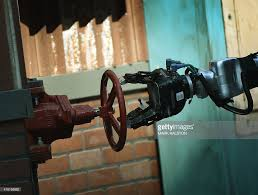
\includegraphics[height=3cm]{darpa/valve.jpeg}\\[0.2cm]
  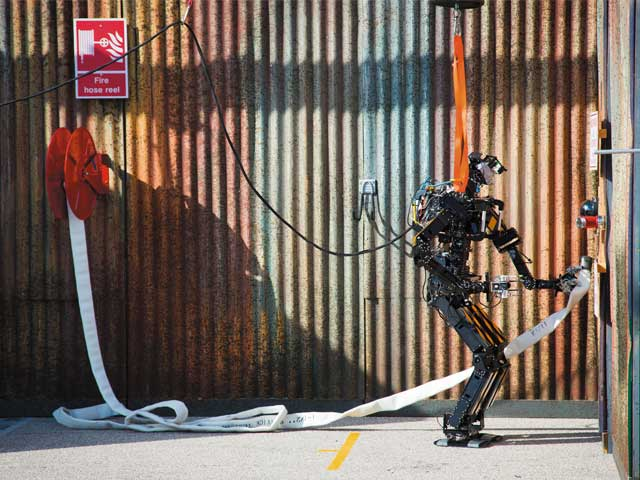
\includegraphics[height=3cm]{darpa/hose.jpg}
\end{center}
%\begin{itemize}
%  \item 
%\end{itemize}
\end{frame}





% ======================================================================
% authorpart.tex
% Copyright (c) Markus Kohm, 2002-2012
%
% This file is part of the LaTeX2e KOMA-Script bundle.
%
% This work may be distributed and/or modified under the conditions of
% the LaTeX Project Public License, version 1.3c of the license.
% The latest version of this license is in
%   http://www.latex-project.org/lppl.txt
% and version 1.3c or later is part of all distributions of LaTeX 
% version 2005/12/01 or later and of this work.
%
% This work has the LPPL maintenance status "author-maintained".
%
% The Current Maintainer and author of this work is Markus Kohm.
%
% This work consists of all files listed in manifest.txt.
% ----------------------------------------------------------------------
% authorpart.tex
% Copyright (c) Markus Kohm, 2002-2012
%
% Dieses Werk darf nach den Bedingungen der LaTeX Project Public Lizenz,
% Version 1.3c, verteilt und/oder veraendert werden.
% Die neuste Version dieser Lizenz ist
%   http://www.latex-project.org/lppl.txt
% und Version 1.3c ist Teil aller Verteilungen von LaTeX
% Version 2005/12/01 oder spaeter und dieses Werks.
%
% Dieses Werk hat den LPPL-Verwaltungs-Status "author-maintained"
% (allein durch den Autor verwaltet).
%
% Der Aktuelle Verwalter und Autor dieses Werkes ist Markus Kohm.
% 
% Dieses Werk besteht aus den in manifest.txt aufgefuehrten Dateien.
% ======================================================================
%
% First part: KOMA-Script for Authors
% Maintained by Markus Kohm
%
% ----------------------------------------------------------------------
%
% Erster Teil: KOMA-Script f�r Autoren
% Verwaltet von Markus Kohm
%
% ======================================================================

\ProvidesFile{authorpart.tex}[2008/05/06 Part KOMA-Script for Authors]

\setpartpreamble{%
  \vspace*{2\baselineskip}%
  \setlength{\parindent}{1em}%

  \noindent In diesem Teil sind die Informationen f�r die Autoren von
  Artikeln, Berichten, B�chern und Briefen zu finden. Dabei wird davon
  ausgegangen, dass der normale Anwender sich weniger daf�r interessiert, wie
  in \KOMAScript{} die Dinge implementiert sind und wo die Schwierigkeiten
  dabei liegen. Auch ist es f�r den normalen Anwender wenig interessant,
  welche obsoleten Optionen und Anweisungen noch enthalten sind. Er will
  wissen, wie er aktuell etwas erreichen kann. Eventuell ist er noch an
  typografischen Hintergrundinformationen interessiert.

  Die wenigen Passagen, die weiterf�hrende Informationen und Begr�ndungen
  enthalten und deshalb f�r ungeduldige Leser weniger von Interesse sind,
  wurden in diesem Teil in serifenloser Schrift gesetzt und k�nnen bei Bedarf
  �bersprungen werden. Wer hingegen noch mehr Informationen zu Hintergr�nden
  der Implementierung, Nebenwirkungen bei Verwendung anderer Pakete und
  zu obsoleten Optionen oder Anweisungen sucht, sei auf
  \autoref{part:forExperts} ab \autopageref{part:forExperts}
  verwiesen. Dar�ber hinaus besch�ftigt sich jener Teil von \KOMAScript{} auch
  mit all den M�glichkeiten, die speziell f�r Autoren von Paketen und Klassen
  geschaffen wurden.  
}

\part{\KOMAScript{} f�r Autoren}
\label{part:forAuthors}

\endinput

%%% Local Variables:
%%% mode: latex
%%% coding: iso-latin-1
%%% TeX-master: "guide.tex"
%%% End:

% ======================================================================
% typearea.tex
% Copyright (c) Markus Kohm, 2001-2015
%
% This file is part of the LaTeX2e KOMA-Script bundle.
%
% This work may be distributed and/or modified under the conditions of
% the LaTeX Project Public License, version 1.3c of the license.
% The latest version of this license is in
%   http://www.latex-project.org/lppl.txt
% and version 1.3c or later is part of all distributions of LaTeX 
% version 2005/12/01 or later and of this work.
%
% This work has the LPPL maintenance status "author-maintained".
%
% The Current Maintainer and author of this work is Markus Kohm.
%
% This work consists of all files listed in manifest.txt.
% ----------------------------------------------------------------------
% typearea.tex
% Copyright (c) Markus Kohm, 2001-2015
%
% Dieses Werk darf nach den Bedingungen der LaTeX Project Public Lizenz,
% Version 1.3c, verteilt und/oder veraendert werden.
% Die neuste Version dieser Lizenz ist
%   http://www.latex-project.org/lppl.txt
% und Version 1.3c ist Teil aller Verteilungen von LaTeX
% Version 2005/12/01 oder spaeter und dieses Werks.
%
% Dieses Werk hat den LPPL-Verwaltungs-Status "author-maintained"
% (allein durch den Autor verwaltet).
%
% Der Aktuelle Verwalter und Autor dieses Werkes ist Markus Kohm.
% 
% Dieses Werk besteht aus den in manifest.txt aufgefuehrten Dateien.
% ======================================================================
%
% Chapter about typearea of the KOMA-Script guide
% Maintained by Markus Kohm
%
% ----------------------------------------------------------------------
%
% Kapitel ueber typearea in der KOMA-Script-Anleitung
% Verwaltet von Markus Kohm
%
% ======================================================================

\KOMAProvidesFile{typearea.tex}%
                 [$Date: 2015-09-04 17:26:05 +0200 (Fri, 04 Sep 2015) $
                  KOMA-Script guide (chapter: typearea)]
\translator{Markus Kohm\and Gernot Hassenpflug\and Krickette Murabayashi}

% Date of translated german file: 2015-09-04

\chapter{Construction of the Page Layout with \Package{typearea}}
\labelbase{typearea}

Many {\LaTeX} classes, including the standard classes, present the user
with the largely fixed configuration of margins and typearea. With the
standard classes, the configuration determined is very much dependent
on the chosen font size. There are
separate packages, such as
\Package{geometry}\IndexPackage{geometry} (see
\cite{package:geometry}), which give the user complete control, but
also full responsibility, of the settings of typearea and margins.

\KOMAScript{} takes a somewhat different approach with its
\Package{typearea} package. Here the user is given several
construction setting and automatization possibilities based on
established typography standards in order to help guide him or her in
making a good choice.

It should be noted that the \Package{typearea} package makes use of
the \Package{scrbase} package. The latter is explained in the expert
section \iffree{of this document}{of this book} in
\autoref{cha:scrbase} from \autopageref{cha:scrbase} onwards. The
majority of the rules documented there are however not directed at the
user, but rather at authors of classes and packages. 


\section{Fundamentals of Page Layout}
\seclabel{basics}

\begin{Explain}
  If you look at a single page of a book or other printed materials,
  you will see that it consists of top, bottom, left, and right
  margins, a (running) head area, the text block, and a (running) foot
  area.  There is also a space between the head area and the text
  block, and between the text block and the foot area. The relations
  between these areas are called the \emph{page
    layout}.\Index[indexmain]{page layout}

%%
%% GH: sollte man schon Hinweise zum Buch hineinarbeiten? Auskommentiert?
%%  \ifx\BUCH\undefined\cite{DANTE:TK0402:MJK}\else(siehe
%%   \autoref{cha:typeareaconstruction})\fi
  The literature contains much discussion of different algorithms and
  heuristic approaches for constructing a good page layout%
  \iffree{ \cite{DANTE:TK0402:MJK}}{. A short introduction to the basics may
    be found at \autoref{cha:typeareaconstruction}}%
  .  Often mentioned is an approach which involves diagonals and their
  intersections. The result is a page where the text block proportions are
  related to the proportions of the \emph{page}.  In a single-sided document,
  the left and the right margin should have equal widths.  The relation of the
  upper margin to the lower margin should be 1\(:\)2. In a double-sided
  document\Index{double-sided} (e.\,g. a book) however, the complete inner
  margin (the margin at the spine) should be the same as each of the two outer
  margins; in other words, a single page contributes only half of the inner
  margin.

  In the previous paragraph, we mentioned and emphasized \emph{the
    page}. Erroneously, it is often thought that with the page format
  the page is the same as the paper format.\Index[indexmain]{paper
    format} However, if you look at a bound document, it is obvious
  that part of the paper vanishes in the
  binding\Index[indexmain]{binding} and is no longer part of the
  visible page. For the page layout, it is not the format of the paper
  which is important, it is the impression of the visible page to the
  reader. Therefore, it is clear that the calculation of the page
  layout must account for the ``lost'' paper in the binding and add
  this amount to the width of the inner margin. This is called the
  \emph{binding correction}.\Index[indexmain]{binding correction} The
  binding correction is therefore calculated as part of the
  \emph{gutter}\Index[indexmain]{gutter}, not % however of
  the visible
  inner margin.

  The binding correction depends on the process of actually
  producing the document and thus cannot be calculated in general.
  Every production process needs its own parameter. In professional
  binding, this parameter is not too important since the printing is
  done on oversized paper which is then cropped to the right size.
  The cropping is done in a way so that the relations for the
  visible double-sided page are as explained above.

  Now we know about the relations of the individual parts of a page.
  However, we do not yet know about the width and the height of the
  text block. Once we know one of these values, we can calculate
  all the other values from the paper format and the page format or
  the binding correction.
  \begin{align*}
    \Var{textblock~height} \Index{textblock height} : \Var{textblock~width} &=
    \Var{page~height}\Index{page} : \Var{page~width}\\
    \Var{top~margin}\Index{margin} : \Var{foot~margin} &=
      \text{1} : \text{2} \\
%
    \Var{left~margin} : \Var{right~margin} &=  \text{1} : \text{1} \\
%
    \Var{half~inner~margin} : \Var{outer~margin} &= \text{1} : \text{2} \\
%
   \Var{page~width} &= 
      \Var{paper~width}\Index{paper} - 
      \Var{binding~correction}\Index{binding correction}\\
%
    \Var{top~margin} + \Var{bottom~margin} &=
    \Var{page~height} - \Var{textblock~height} \\
%
    \Var{left~margin} + \Var{right~margin} &=
    \Var{page~width} - \Var{textblock~width} \\
%
    \Var{half~inner~margin} + \Var{outer~margin} &=
    \Var{page~width} - \Var{textblock~width} \\
%
    \Var{half~inner~margin} + \Var{binding~correction} &=
    \Var{gutter}\Index{gutter}
  \end{align*}
  \Index[indexmain]{margin}%
  The values \Var{left~margin} and \Var{right~margin} only exist in a
  single-sided document while \Var{half~inner~margin} and
  \Var{outer~margin} only exist in a double-sided document.  In these
  equations, we work with \Var{half~inner~margin} since the full inner
  margin belongs to a double-page. Thus, one page has only half of the
  inner margin, \Var{half~inner~margin}.

  The question of the width of the textblock is also discussed in
  the literature. The optimum width depends on several factors:
  \begin{itemize}
  \item size, width, type of the font used
  \item line spacing
  \item word length
  \item available room
  \end{itemize}
  The importance of the font becomes clear once you think about the
  meaning of serifs. Serifs\Index[indexmain]{serifs} are fine strokes
  finishing off the lines of the letters. Letters whose main strokes
  run orthogonal to the text line disturb the flow rather than keeping
  and leading the eye along the line. Those letters then have serifs
  at the ends of the vertical strokes so that the horizontal serifs
  can help lead the eye horizontally. In addition, they help the eye
  to find the beginning of the next line more quickly. Thus, the line
  length for a serif font can be slightly longer than for a sans serif
  font.

  With leading\Index[indexmain]{leading} is meant the vertical
  distance between individual lines of text. In {\LaTeX}, the leading
  is set at about 20\% of the font size. With commands like
  \Macro{linespread}\IndexCmd{linespread} or, better, packages like
  \Package{setspace}\IndexPackage{setspace} (see
  \cite{package:setspace}), the leading can be changed. A wider
  leading helps the eye to follow the line. A very wide leading, on
  the other hand, disturbs reading because the eye has to move a wide
  distance between lines. Also, the reader becomes uncomfortable
  because of the visible stripe effect. The uniform gray value of the
  page is thereby spoiled. Still, with a wider leading, the lines can
  be longer.

  The literature gives different values for good line
  lengths\Index[indexmain]{line length}, depending on the author. To
  some extent, this is related to the native language of the
  author. Since the eye jumps from word to word, short words make this
  task easier. Considering all languages and fonts, a line length of
  60 to 70 characters, including spaces and punctuation, forms a
  usable compromise. This requires well-chosen leading, but {\LaTeX}'s
  default is usually good enough. Longer line lengths should only be
  considered for highly-developed readers who spend several hours
  daily reading. However, even for such readers, line lengths greater than 80
  characters are unsuitable. In any case, the leading must be
  appropriately chosen. An extra 5\% to 10\% is recommended as a good
  rule of thumb. With fonts such as Palatino, which require some 5\%
  more leading even at normal line lengths, even more can be
  required.

  Before looking at the actual construction of the page layout, there
  are just some minor things left to know. {\LaTeX} does not start the
  first line in the text block of a page at the upper edge of the text
  block, but sets the baseline at a defined distance from the top of
  the text block. Also, {\LaTeX} knows the commands
  \Macro{raggedbottom}\IndexCmd{raggedbottom} and
  \Macro{flushbottom}\IndexCmd{flushbottom}. \Macro{raggedbottom}
  specifies that the last line of a page should be positioned wherever
  it was calculated. This means that the position of this line can be
  different on each page, up to the height of one line\,---\,in
  combination of the end of the page with titles, figures, tables or
  similar, even more. In double-sided documents this is usually
  undesirable. \Macro{flushbottom} makes sure that the last line is
  always at the lower edge of the text block. To achieve this,
  {\LaTeX} sometimes needs to stretch vertical glue more than
  allowed. Paragraph skip is such a stretchable, vertical glue, even
  when set to zero.  In order to not stretch the paragraph skip on
  normal pages where it is the only stretchable glue, the height of
  the text block should be set to a multiple of the height of the text
  line, including the distance from the upper edge of the text block
  to the first line.

  This concludes the introduction to page layout as handled by
  {\KOMAScript}. Now, we can begin with the actual construction.
\end{Explain}


\section{Page Layout Construction by Dividing}
\seclabel{divConstruction}

\begin{Explain}
  The easiest way to make sure that the text area has the same ratios
  as the page is as follows:
  \begin{itemize}
  \item First, subtract the part \Var{BCOR}, required for the binding
    correction\Index{binding correction}, from the inner edge of the paper,
    and divide the rest of the page vertically into \Var{DIV} rows of equal
    height.
  \item Next, divide the page horizontally into the same number (\Var{DIV}) of
    columns.
  \item Then, take the uppermost row as the upper margin and the two lowermost
    rows as the lower margin. If you are printing double-sided, you similarly
    take the innermost column as the inner margin and the two outermost
    columns as the outer margin.
  \item Then add the binding correction \Var{BCOR} to the inner margin.
  \end{itemize}
  What now remains of the page is the text area.\Index{text area} The width
  and the height of the text area and margins result automatically from the
  number of rows and columns \Var{DIV}. Since the margins always need three
  stripes, \Var{DIV} must be necessarily greater than three. In order that the
  text area occupy at least twice as much space as the margins, \Var{DIV}
  should really be equal to or greater than 9. With this value, the
  construction is also known as the \emph{classical division factor of 9} (see
  \autoref{fig:typearea.nineparts}).

  \begin{figure}
    \centering
    \setlength{\unitlength}{.25mm}
    \definecolor{komalight}{gray}{.75}
    \definecolor{komamed}{gray}{.6}
    \definecolor{komadark}{gray}{.3}
    \begin{picture}(420,297)
      % BCOR
      \put(198,0){\color{komalight}\rule{24\unitlength}{297\unitlength}}
      \multiput(198,2)(0,20){15}{\thinlines\line(0,1){10}}
      \multiput(222,2)(0,20){15}{\thinlines\line(0,1){10}}
      % the paper
      \put(0,0){\thicklines\framebox(420,297){}}
%      \put(210,0){\thicklines\framebox(210,297){}}
      % the page layout
      \put(44,66){\color{komamed}\rule{132\unitlength}{198\unitlength}}
      \put(244,66){\color{komamed}\rule{132\unitlength}{198\unitlength}}
      % helper lines
      \multiput(0,33)(0,33){8}{\thinlines\line(1,0){198}}
      \multiput(222,33)(0,33){8}{\thinlines\line(1,0){198}}
      \multiput(22,0)(22,0){8}{\thinlines\line(0,1){297}}
      \multiput(244,0)(22,0){8}{\thinlines\line(0,1){297}}
      % annotations
      \put(198,0){\color{white}\makebox(24,297)[c]{%
          \rotatebox[origin=c]{-90}{binding correction}}}
      \put(44,66){\color{white}\makebox(132,198)[c]{page layout left}}
      \put(244,66){\color{white}\makebox(132,198)[c]{page layout right}}
      % box numbers
      \makeatletter
      \multiput(1,27)(0,33){9}{\footnotesize\makebox(0,0)[l]{\the\@multicnt}}
      \multiput(177,291)(-22,0){9}{%
        \footnotesize\makebox(0,0)[l]{\the\@multicnt}}
      \multiput(419,27)(0,33){9}{%
        \footnotesize\makebox(0,0)[r]{\the\@multicnt}}
      \multiput(243,291)(22,0){8}{%
        \footnotesize\makebox(0,0)[r]{\the\numexpr\@multicnt+1\relax}}
      \makeatother
    \end{picture}
    \caption{Double-sided layout with the box construction of the classical division factor of 9, after subtraction of a binding correction}
    \label{fig:typearea.nineparts}
  \end{figure}

  In {\KOMAScript}, this kind of construction is implemented in the
  \Package{typearea} package, where the bottom margin may drop any
  fractions of a line in order to conform with the minor condition for
  the text area height mentioned in the previous paragraph, and
  thereby to minimize the mentioned problem with
  \Macro{flushbottom}. For A4 paper, \Var{DIV} is predefined according
  to the font size (see \autoref{tab:typearea.div},
  \autopageref{tab:typearea.div}). If there is no binding correction
  (\(\Var{BCOR} = 0\Unit{pt}\)), the results roughly match the values
  of \autoref{tab:typearea.typearea},
  \autopageref{tab:typearea.typearea}.

  In addition to the predefined values, one can specify \Var{BCOR} and
  \Var{DIV} as options when loading the package (see
  \autoref{sec:typearea.options}, from
  \autopageref{sec:typearea.typearea} onwards). There is also a
  command to explicitly calculate the type area by providing these
  values as parameters (also see \autoref{sec:typearea.options},
  \autopageref{desc:typearea.cmd.typearea}).

  The \Package{typearea} package can automatically determine the
  optimal value of \Var{DIV} for the font and leading used.
  Again, see \autoref{sec:typearea.options},
  \autopageref{desc:typearea.option.DIV.calc}.
\end{Explain}


\section{Page Layout Construction by Drawing a Circle}
\seclabel{circleConstruction}

\begin{Explain}
  In addition to the page layout construction\Index{page layout}
  method previously described, a somewhat more classical method can be
  found in the literature. The aim of this method is not only to
  obtain identical ratios in the page proportions, but it is
  considered optimal when the height of the text block is the same as
  the width of the page. The exact method is described in
  \cite{JTsch87}.

  A disadvantage of this late Middle Age method is that the width of
  the text area is no longer dependent on the font. Thus, one does not
  choose the text area to match the font, but the author or typesetter
  has to choose the font according to the text area. This can be
  considered a ``must''.

  In the \Package{typearea} package this construction is changed
  slightly. By using a special (normally meaningless) \Var{DIV} value
  or a special package option, a \Var{DIV} value is chosen to match
  the perfect values of the late Middle Age method as closely as
  possible. See also \autoref{sec:typearea.options},
  \autopageref{desc:typearea.option.DIV.calc}.
\end{Explain}

\LoadCommon{0}

\LoadCommon{1}% TODO: Translate!

\section{Options and Macros to Influence the Page Layout}
\seclabel{typearea}

The package \Package{typearea} offers two different user interfaces to
influence type area construction. The more important method is to load
the package with options. For information on how to load packages and
to give package options, please refer to the {\LaTeX} literature,
e.\,g.  \cite{lshort} and \cite{latex:usrguide}, or the examples given
here.  Since the \Package{typearea} package is loaded automatically
when using the {\KOMAScript} main classes, the package options can be
given as class options (see \autoref{sec:maincls.options}).

In this section the \Class{protocol} class will be used, not an
existing {\KOMAScript} class but a hypothetical one. This\iffree{
  documentation}{ book} assumes that ideally there exists a class for
every specific task.

\BeginIndex{Option}{BCOR~=\PName{value}}%
\begin{Declaration}
  \KOption{BCOR}\PName{correction}
\end{Declaration}%
With the aid of the option
\KOption{BCOR}\PName{correction}\ChangedAt{v3.00}{\Package{typearea}}
one may specify the absolute value of the binding
correction\Index{binding correction}, i.\,e., the width of the area
which will be lost from the paper width in the binding process. This
value is then automatically taken into account in the page layout
construction and in the final output is added to the inner (or the
left) margin. For the \PName{correction} specification any measurement
unit understood by \TeX{} is valid.

\begin{Example}
  Assume one is creating a financial report, which should be printed
  out single-sided on A4 paper, and finally kept in a clamp
  folder. The clamp will hide 7.5\Unit{mm}. The stack of pages is very
  thin, thus through paging at most another 0.75\Unit{mm} will be
  lost. Therefore, one may write:
\begin{lstcode}
  \documentclass[a4paper]{report}
  \usepackage[BCOR=8.25mm]{typearea}
\end{lstcode}
  or
\begin{lstcode}
  \documentclass[a4paper,BCOR=8.25mm]{report}
  \usepackage{typearea}
\end{lstcode}
  when using \Option{BCOR} as a global option.

  When using a {\KOMAScript} class, the explicit loading of the
  \Package{typearea} package can be omitted:
\begin{lstcode}
  \documentclass[BCOR=8.25mm]{scrreprt}
\end{lstcode}
  The option \Option{a4paper} could be omitted with \Class{scrreprt},
  since this is a predefined setting for all {\KOMAScript} classes.

  If the option is only later set to a new value, one may then use,
  for example, the following:
\begin{lstcode}
  \documentclass{scrreprt}
  \KOMAoptions{BCOR=8.25mm}
\end{lstcode}
  Thus, at the loading of the \Class{scrreprt} class standard settings
  will be used. When changing the setting with the use of the command
  \Macro{KOMAoptions} or \Macro{KOMAoption} a new page layout with new
  margins will automatically be calculated.
\end{Example}

Please note that when using this option with one of the {\KOMAScript}
classes as in the example above, it must be used either as a class
option, or passed via \Macro{KOMAoptions} or \Macro{KOMAoption} after
loading the class. The \Package{typearea} package should neither be
loaded explicitly with \Macro{usepackage} when using a {\KOMAScript}
class, nor should the option be given as an optional argument
thereto. If the option is changed via \Macro{KOMAoptions} or
\Macro{KOMAoption} after loading the package, the textblock and
margins are automatically recalculated anew.%
%
\EndIndex{Option}{BCOR~=\PName{value}}

\BeginIndex{Option}{DIV~=\PName{value}}%
\begin{Declaration}
  \KOption{DIV}\PName{Factor}
\end{Declaration}%
With the aid of the option
\KOption{DIV}\PName{Factor}\ChangedAt{v3.00}{\Package{typearea}} the
number of stripes into which the page is divided horizontally and
vertically during the page layout construction is set. The exact
construction method is found in
\autoref{sec:typearea.divConstruction}. Of importance is that the
larger the \PName{Factor}, the larger the text block and the smaller
the margins. Any integer value greater than 4 is valid for
\PName{Factor}. Please note that large values can lead to
unfulfillment of various minor conditions in the type area, depending
on further options chosen. Thus, in an extreme case, the header may
fall outside of the page. Users applying the option
\KOption{DIV}\PName{Factor} are themselves responsible for fulfillment
of the marginal conditions and setting of a typographically aesthetic
line length.

In \autoref{tab:typearea.typearea} are found the type area sizes for
several \Var{DIV} factors for an A4 page without binding correction. Here
the minor conditions dependent on font size are not considered.

\begin{table}
  \centering
  \caption[{Type area dimensions dependent on \Var{DIV} for A4}]{Type area
    dimensions dependent on \Var{DIV} for A4 regardless of \Length{topskip}}
  \begin{tabular}{ccccc}
    \toprule
    & 
    \multicolumn{2}{c}{Type area} & \multicolumn{2}{c}{Margins}\\
    %\raisebox{1.5ex}[0pt]{
      \Var{DIV}
    %} 
    & 
    width [mm] & height [mm] & top [mm] & inner [mm] \\
    \midrule
    6  & 105.00 & 148.50 & 49.50 & 35.00 \\
    7  & 120.00 & 169.71 & 42.43 & 30.00 \\
    8  & 131.25 & 185.63 & 37.13 & 26.25 \\
    9  & 140.00 & 198.00 & 33.00 & 23.33 \\
    10 & 147.00 & 207.90 & 29.70 & 21.00 \\
    11 & 152.73 & 216.00 & 27.00 & 19.09 \\
    12 & 157.50 & 222.75 & 24.75 & 17.50 \\
    13 & 161.54 & 228.46 & 22.85 & 16.15 \\
    14 & 165.00 & 233.36 & 21.21 & 15.00 \\
    15 & 168.00 & 237.60 & 19.80 & 14.00 \\
    \bottomrule
  \end{tabular}
  \label{tab:typearea.typearea}
\end{table}

\iffree{}{\clearpage}%
\begin{Example}
  Assume one wants to write a meeting protocol, using the
  \Class{protocol} class. The document should be double-sided. In the
  company 12\Unit{pt} Bookman font is used. This font, which belongs
  to the standard PostScript fonts, is activated in {\LaTeX} with the
  command \verb|\usepackage{bookman}|.  The Bookman font is a very
  wide font, meaning that the individual characters have a large width
  relative to their height. Therefore, the predefined value for
  \Var{DIV} in \Package{typearea} is insufficient. Instead of the
  value of 12 it appears after thorough study of this entire chapter
  that a value of 15 should be most suitable.  The protocol will not
  be bound but punched and kept in a folder. Thus, no binding
  correction is necessary.  One may then write:
\begin{lstcode}
    \documentclass[a4paper,twoside]{protocol}
    \usepackage{bookman}
    \usepackage[DIV=15]{typearea}
\end{lstcode}
  On completion, it is decided that the protocols will from now on be
  collected and bound quarterly into book format. The binding is to be
  a simple glue binding, because it is only done to conform with
  ISO\,9000 and nobody is actually going to read them. For the binding
  including space lost in turning the pages, an average of 12\Unit{mm}
  is required. Thus, one may change the options of the
  \Package{typearea} package accordingly, and use the class for
  protocols conforming to ISO\,9000 regulations:
\begin{lstcode}
  \documentclass[a4paper,twoside]{iso9000p}
  \usepackage{bookman}
  \usepackage[DIV=15,BCOR=12mm]{typearea}
\end{lstcode}
  Of course, it is equally possible to use here a {\KOMAScript} class:
\begin{lstcode}
  \documentclass[twoside,DIV=15,BCOR=12mm]{scrartcl}
  \usepackage{bookman}
\end{lstcode}
  The \Option{a4paper} option can be left out when using the
  \Class{scrartcl} class, as it is predefined in all {\KOMAScript}
  classes.
\end{Example}

Please note that when using the \Option{DIV} option with one of the
{\KOMAScript} classes as in the example above, it must be used either
as a class option, or passed via \Macro{KOMAoptions} or
\Macro{KOMAoption} after loading the class. The \Package{typearea}
package should neither be loaded explicitly with \Macro{usepackage}
when using a {\KOMAScript} class, nor should the option be given as an
optional argument thereto. If the option is changed via
\Macro{KOMAoptions} or \Macro{KOMAoption} after loading the package,
the textblock and margins are automatically recalculated anew.%

\BeginIndex{Option}{DIV~=classic}%
\BeginIndex{Option}{DIV~=calc}%
\begin{Declaration}
  \OptionValue{DIV}{calc}\\
  \OptionValue{DIV}{classic}
\end{Declaration}%
As\ChangedAt{v3.00}{\Package{typearea}} already mentioned in
\autoref{sec:typearea.divConstruction}, for A4 paper there are fixed
predefined settings for the \Var{DIV} value. These can be found in
\autoref{tab:typearea.div}. If a different paper format is chosen,
then the \Package{typearea} package independently calculates an
appropriate \Var{DIV} value.  Of course this same calculation can be
applied also to A4. To obtain this result, one simply uses the
\OptionValue{DIV}{calc} option in place of the
\KOption{DIV}\PName{Factor} option. This option can just as easily be
explicity given for other paper formats. If one desires an automatic
calculation, this also makes good sense, since the possibility exists
to configure different predefined settings in a configuration file
(see \autoref{sec:typearea-experts.cfg}). An explicit passing of the
\OptionValue{DIV}{calc} option then overwrites such configuration
settings.

\begin{table}
  \centering
  \caption{\label{tab:typearea.div}Predefined settings of \PName{DIV} for A4}
  \begin{tabular}{lccc}
    \toprule
    base font size: & 10\Unit{pt} & 11\Unit{pt} & 12\Unit{pt} \\
    \Var{DIV}:           &   8  &  10  &  12  \\
    \bottomrule
  \end{tabular}
\end{table}

The classical page layout construction, the Middle Age book design
canon, mentioned in \autoref{sec:typearea.circleConstruction}, is
similarly selectable. Instead of the \KOption{DIV}\PName{Faktor} or
\OptionValue{DIV}{calc} option, one may use the
\OptionValue{DIV}{classic} option. A \Var{DIV} value closest to the
Middle Age book design canon is then chosen.

\begin{Example}
  In the example using the Bookman font with the
  \KOption{DIV}\PName{Factor} option, exactly that problem of choosing
  a more appropriate \Var{DIV} value for the font arose. As a
  variation on that example, one could simply leave the choice of such
  a value to the \Package{typearea} package:
\begin{lstcode}
  \documentclass[a4paper,twoside]{protocol}
  \usepackage{bookman}
  \usepackage[DIV=calc]{typearea}
\end{lstcode}
\end{Example}

Please note that when using this option with one of the {\KOMAScript}
classes as in the example above, it must be used either as a class
option, or passed via \Macro{KOMAoptions} or \Macro{KOMAoption} after
loading the class. The \Package{typearea} package should neither be
loaded explicitly with \Macro{usepackage} when using a {\KOMAScript}
class, nor should the option be given as an optional argument
thereto. If the option is changed via \Macro{KOMAoptions} or
\Macro{KOMAoption} after loading the package, the textblock and
margins are automatically recalculated anew.%
%
\EndIndex{Option}{DIV~=classic}%
\EndIndex{Option}{DIV~=calc}%

\BeginIndex{Option}{DIV~=current}%
\BeginIndex{Option}{DIV~=last}%
\begin{Declaration}
  \OptionValue{DIV}{current}\\
  \OptionValue{DIV}{last}
\end{Declaration}%
Readers\ChangedAt{v3.00}{\Package{typearea}} who have followed the
examples with acuity actually already know how to calculate a
\Var{DIV} value dependent on the chosen font, when a {\KOMAScript}
class is used together with a font package.

\begin{Explain}
  The problem is that the {\KOMAScript} class already loads the
  \Package{typearea} package itself. Thus, it is not possible to pass
  options as optional arguments to \Macro{usepackage}. It would also
  be pointless to pass the \OptionValue{DIV}{calc} option as an
  optional argument to \Macro{documentclass}. This option would be
  evaluated immediately on loading the \Package{typearea} package and
  as a result the text block and margin would be chosen according to
  the {\LaTeX} standard font and not for the later loaded
  font. However, it is quite possible to recalculate the text block
  and margins anew after loading the font, with the aid of
  \Macro{KOMAoptions}\PParameter{DIV=calc} or
  \Macro{KOMAoption}\PParameter{DIV}\PParameter{calc}. Via
  \PValue{calc} an appropriate \Var{DIV} value for a good line length
  is then chosen.

  As it is often more practical to set the \Option{DIV} option not
  after loading the font, but at a more visible point, such as when
  loading the class, the \Package{typearea} package offers two further
  symbolic values for this option.
\end{Explain}

With \KOption{DIV}\PName{current}\ChangedAt{v3.00}{\Package{typearea}}
a renewed calculation of text block and margin is requested, in which
the currently set \Var{DIV} will be used. This is less of interest for
renewed type area calculations after loading a different font; it is
rather more useful for determining, for example, after changing the
leading, while keeping \Var{DIV} the same, that the marginal condition
is fulfilled that \Length{textheight} less
\Length{topskip} is a multiple of \Length{baselineskip}.

With \KOption{DIV}\PName{last}\ChangedAt{v3.00}{\Package{typearea}} a
renewed calculation of text block and margin is requested, where
exactly the same setting is used as in the last calculation.

\begin{Example}
  Let us take up the previous example again, in which a good line
  length is required for a type area using the Bookman font. At the
  same time, a {\KOMAScript} class is to be used. This is easily
  possible using the symbolic value \PValue{last} and the command
  \Macro{KOMAoptions}:
\begin{lstcode}
  \documentclass[BCOR=12mm,DIV=calc,twoside]{scrartcl}
  \usepackage{bookman}
  \KOMAoptions{DIV=last}
\end{lstcode}
If it should later be decided that a different \Var{DIV} value is
required, then only the setting of the optional argument to
\Macro{documentclass} need be changed.
\end{Example}

A summary of all possible symbolic values for the \Option{DIV} option
can be found in \autoref{tab:symbolicDIV}. At this point it is noted
that the use of the \Package{fontenc}\IndexPackage{fontenc} package
can also lead to \LaTeX{} loading a different font.

\begin{table}
  \caption[{Symbolic values for the \Option{DIV} option and the
    \PName{DIV} argument to \Macro{typearea}}]{Possible symbolic values for the \Option{DIV} option or the \PName{DIV} argument to
    \Macro{typearea}\OParameter{BCOR}\Parameter{DIV}}
  \label{tab:symbolicDIV}
  \begin{desctabular}
    \pventry{areaset}{Recalculate page
      layout.\IndexOption{DIV~=areaset}}%
    \pventry{calc}{Recalculate type area including choice of
      appropriate \Var{DIV} value.\IndexOption{DIV~=calc}}%
    \pventry{classic}{Recalculate type area using Middle Age book
      design canon (circle-based
      calculation).\IndexOption{DIV~=classic}}%
    \pventry{current}{Recalculate type area using current \Var{DIV}
      value.\IndexOption{DIV~=current}}%
    \pventry{default}{Recalculate type area using the standard value
      for the current page format and current font size. If no
      standard value exists, \PValue{calc} is
      used.\IndexOption{DIV~=default}}%
    \pventry{last}{Recalculate type area using the same \PName{DIV}
      argument as was used in the last call.\IndexOption{DIV~=last}}%
  \end{desctabular}
\end{table}

Often the renewed type area calculation is required in combination
with a change in the line spacing
(\emph{leading})\Index{leading}. Since the type area should be
calculated such that an integer number of lines fit in the text block,
a change in the leading normally requires a recalculation of the page
layout.
 
\begin{Example}
  For a thesis document, a font of size 10\Unit{pt} and a spacing of
  1.5 lines is required. By default, {\LaTeX} sets the leading for
  10\Unit{pt} at 2\Unit{pt}, in other words 1.2 lines. Therefore, an
  additional stretch factor of 1.25 is needed. Additionally, a binding
  correction of \(12\Unit{mm}\) is stipulated. Then the solution could be
  written as follows:
\begin{lstcode}
  \documentclass[10pt,twoside,BCOR=12mm,DIV=calc]{scrreprt}
  \linespread{1.25}
  \KOMAoptions{DIV=last}
\end{lstcode}\IndexCmd{linespread}
Since \Package{typearea} always executes the command
\Macro{normalsize} itself upon calculation of a new type area, it is
not necessary to activate the chosen leading with \Macro{selectfont}
after \Macro{linespread}, since this will be used already in the
recalculation.

When using the \Package{setspace} package (see
\cite{package:setspace}), the same example would appear as follows:
\begin{lstcode}
  \documentclass[10pt,twoside,BCOR=12mm,DIV=calc]{scrreprt}
  \usepackage{setspace}
  \onehalfspacing
  \KOMAoptions{DIV=last}
\end{lstcode}
As can be seen, with the use of the \Package{setspace} package one no
longer neesds to know the correct stretch value.

At this point it should be noted that the line spacing for the title
page should be reset to the normal value.
\iffalse% Umbruchkorrektur
  A complete example would be:
\fi
\begin{lstcode}
  \documentclass[10pt,twoside,BCOR=12mm,DIV=calc]
                {scrreprt}
  \usepackage{setspace}
  \onehalfspacing
  \AfterTOCHead{\singlespacing}
  \KOMAoptions{DIV=last}
  \begin{document}
  \title{Title}
  \author{Markus Kohm}
  \begin{spacing}{1}
    \maketitle
  \end{spacing}
  \tableofcontents
  \chapter{Ok}
  \end{document}
\end{lstcode}
  See further also the notes in \autoref{sec:typearea.tips}. The command
  \Macro{AfterTOCHead}\IndexCmd{AfterTOCHead} will be described in
  \autoref{cha:tocbasic} of \autoref{part:forExperts} on
  \autopageref{desc:tocbasic.cmd.AfterTOCHead}.
\end{Example}

Please note that when using this option with one of the {\KOMAScript}
classes as in the example above, it must be used either as a class
option, or passed via \Macro{KOMAoptions} or \Macro{KOMAoption} after
loading the class. The \Package{typearea} package should neither be
loaded explicitly with \Macro{usepackage} when using a {\KOMAScript}
class, nor should the option be given as an optional argument
thereto. If the option is changed via \Macro{KOMAoptions} or
\Macro{KOMAoption} after loading the package, the textblock and
margins are automatically recalculated anew.%
%
\EndIndex{Option}{DIV~=current}%
\EndIndex{Option}{DIV~=last}%
\EndIndex{Option}{DIV~=\PName{value}}

\BeginIndex{Cmd}{typearea}%
\BeginIndex{Cmd}{recalctypearea}%
\begin{Declaration}
  \Macro{typearea}\OParameter{BCOR}\Parameter{DIV}\\
  \Macro{recalctypearea}
\end{Declaration}%
\begin{Explain}
  If the \Option{DIV} option or the \Option{BCOR} option is set after
  loading of the \Package{typearea} package, then internally the
  command \Macro{typearea} is called. When setting the \Option{DIV}
  option the symbolic value \PValue{current} is used internally for
  \PName{BCOR}, which for reasons of completeness is found also in
  \autoref{tab:symbolicBCOR}. When setting the \Option{BCOR} option,
  the symbolic value \PValue{last} is used internally for
  \PName{DIV}. If it is instead desired that the text block and
  margins should be recalculated using the symbolic value
  \PValue{current} for \PName{DIV}, then
  \Macro{typearea}\POParameter{current}\PParameter{current} can be used
  directly.
\end{Explain}

\begin{table}
  \caption[{Symoblic \PName{BCOR} arguments for
    \Macro{typearea}}]{Possible symbolic \PName{BCOR} arguments for
    \Macro{typearea}\OParameter{BCOR}\Parameter{DIV}}
  \label{tab:symbolicBCOR}
  \begin{desctabular}
    \pventry{current}{Recalculate type area with the currently valid
      \Var{BCOR} value.\IndexOption{BCOR~=current}}
  \end{desctabular}
\end{table}

If both \PName{BCOR} and \PName{DIV} need changing, then it is
recommended to use \Macro{typearea}, since then the text block and
margins are recalculated only once. With
\Macro{KOMAoptions}\PParameter{\KOption{DIV}\PName{DIV},%
  \KOption{BCOR}\PName{BCOR}} the text block and margins are
recalculated once for the change to \PName{DIV} and again for the
change to \PName{BCOR}.

\begin{Explain}
  The command \Macro{typearea} is currently defined so as to make it
  possible to change the type area anywhere within a
  document. Several assumptions about the structure of the {\LaTeX}
  kernel are however made and internal definitions and sizes of the
  kernel changed. There is a definite possibility, but no guarantee,
  that this will continue to function in future versions of
  \LaTeXe{}. When used within the document, a page break will result.
\end{Explain}

Since \Macro{typearea}\POParameter{current}\PParameter{last} or
\Macro{KOMAoptions}\PParameter{DIV=last} are often needed for
recalculation of the type area, there exists specially the
abbreviated command
\Macro{recalctypearea}\ChangedAt{v3.00}{\Package{typearea}}.

\begin{Example}
  If one finds the notation
\begin{lstcode}
  \KOMAoptions{DIV=last}
\end{lstcode}
  or
\begin{lstcode}
  \typearea[current]{last}
\end{lstcode}
  for the recalculation of text block and margins too complicated for
  reasons of the many special characters, then one may use more simply
  the following.
\begin{lstcode}
  \recalctypearea
\end{lstcode}
\end{Example}%
\EndIndex{Cmd}{recalctypearea}%
\EndIndex{Cmd}{typearea}

\BeginIndex{Option}{twoside~=\PName{simple switch}}%
\BeginIndex{Option}{twoside~=semi}%
\begin{Declaration}
  \KOption{twoside}\PName{simple switch}\\
  \OptionValue{twoside}{semi}
\end{Declaration}%
As already explained in \autoref{sec:typearea.basics}, the margin
configuration is dependent on whether the document is to be typeset
single- or double-sided. For single-sided typesetting, the left and
right margins are equally wide, whereas for double-sided printing the
inner margin of one page is only half as wide as the corresponding
outer margin. In order to implement this distinction, the
\Package{typearea} package must be given the \Option{twoside} option,
if the document is to be typeset double-sided. Being a \PName{simple switch},
any of the standard values for simple switches in
\autoref{tab:truefalseswitch} are valid. If the option is passed
without a value, the value \PValue{true} is assumed, so double-sided
typesetting is carried out. Deactivation of the option leads to
single-sided typesetting.

\begin{table}
  \centering
  \caption{Standard values for simple switches in \KOMAScript}
  \begin{tabular}{ll}
    \toprule
    Value & Description \\
    \midrule
    \PValue{true} & activates the option \\
    \PValue{on}   & activates the option \\
    \PValue{yes}  & activates the option \\
    \PValue{false}& deactivates the option \\
    \PValue{off}  & deactivates the option \\
    \PValue{no}   & deactivates the option \\
    \bottomrule
  \end{tabular}
  \label{tab:truefalseswitch}
\end{table}

Apart from the values in \autoref{tab:truefalseswitch} the value
\PValue{semi}\ChangedAt{v3.00}{\Package{typearea}} can also be given. The
value \PValue{semi} results in a double-sided typesetting with single-sided
margins and single-sided, i.\ e., not alternating, margin
notes. Nevertheless\ChangedAt{v3.12}{\Package{typearea}}, since \KOMAScript{}
version 3.12 binding corrections (see \Option{BCOR},
\autopageref{desc:typearea.option.BCOR}) will be part of the left margin on
odd pages but part of the right margin on even pages. But if you use
compatibility with prior versions of \KOMAScript (see
\autoref{sec:typearea.compatibilityOptions},
\autopageref{sec:typearea.compatibilityOptions}), binding correction will be
part of the left margin on both pages while using \OptionValue{twoside}{semi}.

The option can also be passed as class option in
\Macro{documentclass}, as package option to \Macro{usepackage}, or
even after loading of the \Package{typearea} package with the use of
 \Macro{KOMAoptions} or \Macro{KOMAoption}. Use of the option after
loading the \Package{typearea} package results automatically in 
recalculation of the type area using \Macro{recalctypearea} (see
\autopageref{desc:typearea.cmd.recalctypearea}). If double-sided
typesetting was active before the option was set, then before the
recalculation a page break is made to the next odd page.%
%
\EndIndex{Option}{twoside~=semi}%
\EndIndex{Option}{twoside~=\PName{simple switch}}

\BeginIndex{Option}{twocolumn~=\PName{simple switch}}%
\begin{Declaration}
  \KOption{twocolumn}\PName{simple switch}
\end{Declaration}
For the calculation of a good type area with the help of
\OptionValue{DIV}{calc} it is useful to know in advance if the
document is to be typeset one-column or two-column. Since the
observations about line length in \autoref{sec:typearea.basics} then
apply to each column, the width of a type area in a two-column
document can be up to double that in a one-column document.

To implement this difference, the \Package{typearea} package must be
told via the \Option{twocolumn} option whether the document is to be
two-column. Since this is a \PName{simple switch}, any of the standard values
for simple switches from \autoref{tab:truefalseswitch} is valid. If
the option is passed without a value, the value \PValue{true} is
assumed, i.\,e., two-column typesetting. Deactivation of the option
results in one-column typesetting.

The option can also be passed as class option in
\Macro{documentclass}, as package option to \Macro{usepackage}, or
even after loading of the \Package{typearea} package with the use of
 \Macro{KOMAoptions} or \Macro{KOMAoption}. Use of the option after
loading the \Package{typearea} package results automatically in 
recalculation of the type area using \Macro{recalctypearea} (see
\autopageref{desc:typearea.cmd.recalctypearea}).%
%
\EndIndex{Option}{twocolumn~=\PName{simple switch}}


\BeginIndex{Option}{headinclude~=\PName{simple switch}}%
\BeginIndex{Option}{footinclude~=\PName{simple switch}}%
\begin{Declaration}
  \KOption{headinclude}\PName{simple switch}\\
  \KOption{footinclude}\PName{simple switch}
\end{Declaration}%
\begin{Explain}%
  So far we have discussed how the type area is
  calculated\Index{type area} and the relationship of the
  margins\Index{margins} to one another and between margins and text
  block. However, one important question has not been answered: What
  constitutes the margins?

  At first glance the question appears trivial: Margins are those
  parts on the right, left, top and bottom which remain empty. But
  this is only half the story. Margins are not always empty. There may
  be margin notes, for example (see \Macro{marginpar} command in
  \cite{lshort} or \autoref{sec:maincls.marginNotes}).

  One could also ask whether headers\Index{page header} and
  footers\Index{page footer} belong to the upper and lower margins or
  to the text. This can not be answered unambiguously. Of course an
  empty footer or header belongs to the margins, since they can not be
  distinguished from the rest of the margin. A header or footer that
  contains only a page
  number\Index[indexmain]{pagination}\footnote{Pagination refers to
    the indication of the page number.} will optically appear more
  like a margin. For the optical appearance it is not important
  whether headers or footers are easily recognized as such during
  reading.  Of importance is only how a well-filled page appears when
  viewed \emph{out of focus}. One could use the glasses of one's
  far-sighted grandparents, or, lacking those, adjust one's vision to
  infinity and look at the page with one eye only. Those wearing
  spectacles will find this much easier, of course.  If the footer
  contains not only the page number, but other material like a
  copyright notice, it will optically appear more like a part of the
  text body.  This needs to be taken into account when calculating
  text layout.

  For the header this is even more complicated. The header frequently
  contains running headings\Index[indexmain]{running
    headings}.\footnote{Running headings refer to the repetition of a
    title in titling font, which is more often typeset in the page
    header, less often in the page footer.}  In the case of running
  headings with long chapter and section titles, the header lines will
  be very long and appear to be part of the text body.  This effect
  becomes even more significant when the header contains not only the
  chapter or section title but also the page number. With material on
  the right and left side, the header will no longer appear as an
  empty margin. It is more difficult if the pagination is in the
  footer, and the length of the titles varies so that the header may
  appear as a margin on one page and as text on another.  However,
  these pages should not be treated differently under any
  circumstances, as this would lead to vertically jumping headers. In
  this case it is probably best to count the header as part of the
  text.

  The decision is easy when text and header or footer are separated
  from the text body by a line. This will give a ``closed'' appearance
  and header or footer become part of the text body.  Remember: It is
  irrelevant that the line improves the optical separation of text and
  header or footer; only the appearance when viewed out
  of focus is important.
\end{Explain}

The \Package{typearea} package cannot make the decision whether or
not to count headers and footers as part of the text body or the
margin. Options \Option{headinclude} and \Option{footinclude} cause
the header or footer to be counted as part of the text.  These
options, being a \PName{simple switch}\ChangedAt{v3.00}{\Package{typearea}},
understand the standard values for simple switches in
\autoref{tab:truefalseswitch}. One may use the options without
specifying a value, in which case the value \PValue{true} is used for
the \PName{simple switch}, i.\,e., the header or footer is counted as part of
the text.

Readers who are unsure about the the correct setting should re-read
the above explanations. Default is usually
\OptionValue{headinclude}{false} and \OptionValue{footinclude}{false},
but this can change depending on {\KOMAScript} class and {\KOMAScript}
packages used (see \autoref{sec:maincls.options} and
\autoref{cha:scrlayer-scrpage}).

Please note that when using these options with one of the
{\KOMAScript} classes as in the example above, they must be used
either as a class option, or passed via \Macro{KOMAoptions} or
\Macro{KOMAoption} after loading the class. Changing of these options
after loading the \Package{typearea} package does not result in an
automatic recalculation of the type area. Instead, the changes only
take effect at the next recalculation of the type area. For
recalculation of the type area, refer to the \Option{DIV} option with
the values \PValue{last} or \PValue{current} (see
\autopageref{desc:typearea.option.DIV.last}) or the
\Macro{recalctypearea} command (see
\autopageref{desc:typearea.cmd.recalctypearea}).%
%
\EndIndex{Option}{headinclude~=\PName{simple switch}}%
\EndIndex{Option}{footinclude~=\PName{simple switch}}%


\BeginIndex{Option}{mpinclude~=\PName{simple switch}}%
\begin{Declaration}
  \KOption{mpinclude}\PName{simple switch}
\end{Declaration}
Besides\ChangedAt{v2.8q}{\Class{scrbook}\and \Class{scrreprt}\and
  \Class{scrartcl}} documents where the head and foot are part of the
text area, there are also documents where the margin-note area must be
counted as part of the text body as well.  The option \Option{mpinclude} does
exactly this.  The option, as a
\PName{simple switch}\ChangedAt{v3.00}{\Package{typearea}}, understands the
standard values for simple switches in
\autoref{tab:truefalseswitch}. One may also pass this option without
specifying a value, in which case the value \PValue{true} for
\PName{simple switch} is assumed.

The effect of \OptionValue{mpinclude}{true} is that one width-unit of
the text body is taken for the margin-note area.  Using option
\OptionValue{mpinclude}{false}, the default setting, the normal
margin is used for the margin-note area.  The width of that area is
one or one and a half width-unit, depending on whether one-sided or
double-sided page layout has been chosen.  The option
\OptionValue{mpinclude}{true} is mainly for experts and so is not recommended.
  
\begin{Explain}
  In the cases where the option \Option{mpinclude} is used, often a
  wider margin-note area is required.  In many cases not the whole
  margin-note width should be part of the text area, for example if
  the margin is used for quotations.  Such quotations are typeset as
  ragged text with the flushed side where the text body is.  Since
  ragged text gives no homogeneous optical impression, the long lines
  can reach right into the normal margin.  This can be done using
  option \Option{mpinclude} and by an enlargement of length
  \Length{marginparwidth} after the type area has been set up.  The
  length can be easily enlarged with the command \Macro{addtolength}.
  How much the length has to be enlarged depends on the special
  situation and it requires some flair.  This is another reason the
  \Option{mpinclude} option is primarily left for experts.  Of course
  one can set up the margin-width to reach a third right into the
  normal margin; for example, using
\begin{lstcode}[belowskip=\dp\strutbox]
  \setlength{\marginparwidth}{1.5\marginparwidth}
\end{lstcode}
  gives the desired result.

  Currently there is no option to enlarge the margin by a given
  amount.  The only solution is to either not use the option
  \Option{mpinclude} or to set \Option{mpinclude} to \PValue{false},
  and after the type area has been calculated, one reduces the
  width of the text body \Length{textwidth} and enlarges the margin
  width \Length{marginparwidth} by the same amount.  Unfortunately,
  this cannot be combined with automatic calculation of the
  \PName{DIV} value.  In contrast
  \Option{DIV=calc}\IndexOption{DIV~=calc} (see
  \autopageref{desc:typearea.option.DIV.calc}) heeds
  \Option{mpinclude}.
\end{Explain}

Please note that when using this option with one of the {\KOMAScript}
classes as in the example above, it must be used either as a class
option, or passed via \Macro{KOMAoptions} or \Macro{KOMAoption} after
loading the class. Changing of this option after loading the
\Package{typearea} package does not result in an automatic
recalculation of the type area. Instead, the changes only take effect
at the next recalculation of the type area. For recalculation of the
type area, refer to the \Option{DIV} option with the values
\PValue{last} or \PValue{current} (see
\autopageref{desc:typearea.option.DIV.last}) or the
\Macro{recalctypearea} command (see
\autopageref{desc:typearea.cmd.recalctypearea}).%
%
\EndIndex{Option}{mpinclude~=\PName{simple switch}}%


\BeginIndex{Option}{headlines~=\PName{number}}%
\BeginIndex{Option}{headheight~=\PName{height}}%
\begin{Declaration}
  \KOption{headlines}\PName{number of lines}\\
  \KOption{headheight}\PName{height}
\end{Declaration}%
We have seen how to calculate the type area using the
\Package{typearea} package and how to specify whether header and
footer are part of the text or the margins. However, in particular for
the header, we still have to specify the height. This is achieved with
the options \Option{headlines} and
\Option{headheight}\ChangedAt{v3.00}{\Package{typearea}}.

The option \Option{headlines} is set to the number of header
lines. The \Package{typearea} package uses a default of 1.25. This is
a compromise, large enough for underlined headers (see
\autoref{sec:maincls.options}) and small enough that the relative
weight of the top margin is not affected too much when the header is
not underlined. Thus in most cases you may leave \Option{headlines} at
its default value and adapt it only in special cases.

\begin{Example}
  Assume that you want to use a header with two lines. Normally this would
  result in an ``\texttt{overfull} \Macro{vbox}'' warning for each page. To
  prevent this from happening, the \Package{typearea} package is told to
  calculate an appropriate type area:
\begin{lstcode}
  \documentclass[a4paper]{article}
  \usepackage[headlines=2.1]{typearea}
\end{lstcode}
If you use a {\KOMAScript} class, it is recommended to pass this option
directly as a class option:
\begin{lstcode}
  \documentclass[a4paper,headlines=2.1]{scrartcl}
\end{lstcode}
Commands that can be used to define the contents of a header with two lines
are described in \autoref{cha:scrlayer-scrpage}.
\end{Example}

In some cases it is useful to be able to specify the header height not
in lines but directly as a length measurement. This is accomplished
with the aid of the alternative option \Option{headheight}. For
\PName{height} any lengths and sizes that \LaTeX{} understands are
valid. It should be noted though that when using a \LaTeX{} length
such as \Length{baselineskip} its value at the time of the calculation
of the type area and margins, not at the time of setting of the
option, is decisive.

Please note that when using these options with one of the
{\KOMAScript} classes as in the example above, they must be used
either as a class option, or passed via \Macro{KOMAoptions} or
\Macro{KOMAoption} after loading the class. Changing of these options
after loading the \Package{typearea} package does not result in an
automatic recalculation of the type area. Instead, the changes only
take effect at the next recalculation of the type area. For
recalculation of the type area, refer to the \Option{DIV} option with
the values \PValue{last} or \PValue{current} (see
\autopageref{desc:typearea.option.DIV.last}) or the
\Macro{recalctypearea} command (see
\autopageref{desc:typearea.cmd.recalctypearea}).%
%
\EndIndex{Option}{headheight~=\PName{height}}%
\EndIndex{Option}{headlines~=\PName{number}}

\begin{Declaration}
  \KOption{footlines}\PName{number}\\
  \KOption{footheight}\PName{height}
\end{Declaration}
\BeginIndex{Option}{footlines~=\PName{number}}%
\BeginIndex{Option}{footheight~=\PName{height}}%
As\ChangedAt{v3.12}{\Package{typearea}} well as we needed a height value for
the head, we need a height value for the page footer. But in difference to the
height of the head, \LaTeX itself do not provide a length for the height of
the page footer. So \Package{typearea} defines the new length
\Length{footheight}\IndexLength[indexmain]{footheight}, if it does not
exist. Wether or not this length will be used by classes or packages depends
on the classes and packages, that will be used. The \KOMAScript{} package
\Package{scrlayer-scrpage} incorporates \Length{footheight} and actively
cooperates with \Package{typearea}. The \KOMAScript{} classes do not recognize
\Length{footheight}, because without any package assistance they provide only
page styles with single-line page footers.

You can use \Option{footlines} to setup the \PName{number} of lines in the
page footer, similar to \Option{headlines} for the number of lines in the page
header. By default \Package{typearea} uses 1.25 footlines. This is a
compromise, large enough for overlining or underlining footers and small
enough that the relative weight of the bottom margin is not affected too mich
when the footer is neither over- nor underlined. Thus in most cases you may
leave \PName{footlines} at its default value and adapt it only in special
cases.

\begin{Example}
  Assume a two-lined copyright note should be placed in the page
  footer. Indeed, \LaTeX{} itself does not test, whether or not the footer has
  room enough for that, exceeding of the available height would probably could
  result in unbalanced margins. Moreover, for example package
  \Package{scrlayer-scrpage}, that may be used to define such a page footer,
  would definitely do such a test and would notify a recognised oversize. So
  it makes sense, to declare the needed footheight already for the calculation
  of the text area and the margins:
\begin{lstcode}
  \documentclass[a4paper]{article}
  \usepackage[footlines=2.1]{typearea}
\end{lstcode}
  Again, if you use a \KOMAScript{} class, it is recommended to pass this
  option directly a a class option:
\begin{lstcode}
  \documentclass[footlines=2.1]{scrartcl}
\end{lstcode}
  Commands that can be used to define the contents of a footer with two lines
  are described in \autoref{cha:scrlayer-scrpage}.
\end{Example}

In some cases it is useful to be able to specify the footer height not
in lines but directly as a length measurement. This is accomplished
with the aid of the alternative option \Option{footheight}. For
\PName{height} any lengths and sizes that \LaTeX{} understands are
valid. It should be noted though that when using a \LaTeX{} length
such as \Length{baselineskip} its value at the time of the calculation
of the type area and margins, not at the time of setting of the
option, is decisive.

Please note that when using these options with one of the
{\KOMAScript} classes as in the example above, they must be used
either as a class option, or passed via \Macro{KOMAoptions} or
\Macro{KOMAoption} after loading the class. Changing of these options
after loading the \Package{typearea} package does not result in an
automatic recalculation of the type area. Instead, the changes only
take effect at the next recalculation of the type area. For
recalculation of the type area, refer to the \Option{DIV} option with
the values \PValue{last} or \PValue{current} (see
\autopageref{desc:typearea.option.DIV.last}) or the
\Macro{recalctypearea} command (see
\autopageref{desc:typearea.cmd.recalctypearea}).%
\EndIndex{Option}{footheight~=\PName{height}}%
\EndIndex{Option}{footlines~=\PName{number}}%



\BeginIndex{Cmd}{areaset}%
\begin{Declaration}
  \Macro{areaset}\OParameter{BCOR}\Parameter{Width}\Parameter{Height}
\end{Declaration}%
So far we have seen how a good or even very good
type area\Index{type area} is calculated and how the
\Package{typearea} package can support these calculations, giving you
at the same time the freedom to adapt the layout to your needs.
However, there are cases where the text body has to fit exactly some
specified dimensions. At the same time the margins should be well
spaced and a binding correction should be possible. The
\Package{typearea} package offers the command \Macro{areaset} for this
purpose. As parameters this command accepts the binding correction and
the width and height of the text body.  Width and position of the
margins will then be calculated automatically, taking account of the
options \Option{headinclude}, \OptionValue{headinclude}{false},
\Option{footinclude} and \OptionValue{footinclude}{false} where
needed.  On the other hand, the options
\Option{headlines}\IndexOption{headlines} and
\Option{headheight}\IndexOption{headheight} are ignored!

The default of \PName{BCOR} is 0\Unit{pt}. If you want to re-use the current
binding correction, e.\,g. the value set by option
\Option{BCOR}\IndexOption{BCOR}, you can use the symbolic value
\PValue{current} at the optional argument.

\begin{Example}
  Assume a text, printed on A4 paper, should have a width of exactly 60
  characters of typewriter font and a height of exactly 30 lines. This could
  be achieved as follows:
\begin{lstcode}
  \documentclass[a4paper,11pt]{article}
  \usepackage{typearea}
  \newlength{\CharsLX}% Width of 60 characters
  \newlength{\LinesXXX}% Height of 30 lines
  \settowidth{\CharsLX}{\texttt{1234567890}}
  \setlength{\CharsLX}{6\CharsLX}
  \setlength{\LinesXXX}{\topskip}
  \addtolength{\LinesXXX}{29\baselineskip}
  \areaset{\CharsLX}{\LinesXXX}
\end{lstcode}
You need only 29 instead of 30, because the base line of the topmost
text line is \Macro{topskip} below the top margin of the type area, as
long as the height of the topmost line is less than
\Macro{topskip}. Thus, the uppermost line does not require any
height. The descenders of characters on the lowermost line, on the
other hand, hang below the dimensions of the type area.

\item A poetry book with a square text body with a page length of
  15\Unit{cm} and a binding correction of 1\Unit{cm} could be
  achieved like this:
\begin{lstcode}
  \documentclass{poetry}
  \usepackage{typearea}
  \areaset[1cm]{15cm}{15cm}
\end{lstcode}
\end{Example}
\EndIndex{Cmd}{areaset}

\BeginIndex{Option}{DIV~=areaset}%
\begin{Declaration}
  \OptionValue{DIV}{areaset}
\end{Declaration}%
In\ChangedAt{v3.00}{\Package{typearea}} rare cases it is useful to be
able to reconstruct the current type area anew. This is possible via
the option \OptionValue{DIV}{areaset}, where
\Macro{KOMAoptions}\PParameter{DIV=areaset} corresponds to the 
\begin{lstcode}[belowskip=\dp\strutbox]
  \areaset[current]{\textwidth}{\textheight}
\end{lstcode}
command. The same result is obtained if one uses
\OptionValue{DIV}{last} and the typearea was last set with
\Macro{areaset}.%
%
\EndIndex{Option}{DIV~=areaset}%

The \Package{typearea} package was not made to set up predefined
margin values. If you have to do so you may use package
\Package{geometry}\IndexPackage{geometry} (see
\cite{package:geometry}).


\section{Paper Format Selection}
\seclabel{paperTypes}%
\BeginIndex{}{paper>format}%

The paper format is a definitive characteristic of any document. As
already mentioned in the description of the supported page layout
constructions (see \autoref{sec:typearea.basics} to
\autoref{sec:typearea.circleConstruction} from
\autopageref{sec:typearea.basics} onwards), the entire page division
and document layout depends on the paper format. Whereas the {\LaTeX}
standard classes are restricted to a few formats, {\KOMAScript}
supports in conjunction with the \Package{typearea} package even
exotic paper sizes.


\BeginIndex{Option}{paper~=\PName{format}}%
\BeginIndex{Option}{paper~=\PName{orientation}}%
\begin{Declaration}
  \KOption{paper}\PName{format}
\end{Declaration}%
The option \Option{paper}\ChangedAt{v3.00}{\Package{typearea}} is the
central element for format selection in \KOMAScript.  \PName{Format}
supports first of all the American formats \Option{letter},
\Option{legal}, and \Option{executive}. In addition, it supports the
ISO formats of the series A, B, C, and D, for example \PValue{A4}
or\,---\,written in lowercase\,---\,\PValue{a4}. 

Landscape formats are supported by specifying the option again, this time with
value \PValue{landscape}\Index{paper>orientation} or
\PValue{seascape}\ChangedAt{v3.02c}{\Package{typearea}}. The difference is
that application \File{dvips} rotates at \PValue{landscape} by
-90\Unit{\textdegree}, while it rotates by +90\Unit{\textdegree} at
\PValue{seascape}. So you may use \PValue{seascape} whenever a PostScript
viewer application shows landscape pages upside-down. But you may see the
difference only if you do not deactivate option \Option{pagesize}, which will
be described next.

Additionally, the \PName{format} can also be specified in the form
\PName{height}\texttt{:}\PName{width}. Note that until
version~3.01a\ChangedAt{v3.01b}{\Package{typearea}} \PName{height} and
\PName{width} has been interchanged. 
% You should at least pay attention to this,
This is important
if you use compatibility settings (see option
\Option{version}\IndexOption{version}\important{\Option{version}},
\autoref{sec:typearea.compatibilityOptions},
\autopageref{desc:typearea.option.version}).

\begin{Example}
 Assume one wishes to print on ISO A8 file cards in landscape
 orientation. Margins should be very small, no header or footer
 will be used.
\begin{lstcode}
  \documentclass{article}
  \usepackage[headinclude=false,footinclude=false,
              paper=A8,landscape]{typearea}
  \areaset{7cm}{5cm}
  \pagestyle{empty}
  \begin{document}
  \section*{Supported Paper Sizes}
  letter, legal, executive, a0, a1 \dots\ %
  b0, b1 \dots\ c0, c1 \dots\ d0, d1 \dots
  \end{document}
\end{lstcode}
If the file cards have the special format (height:width)
5\Unit{cm}\,:\,3\Unit{cm}, this can be achieved using the following
code.
\begin{lstcode}
  \documentclass{article}
  \usepackage[headinclude=false,footinclude=false,%
              paper=A8,paper=5cm:3cm]{typearea}
  \areaset{4cm}{2.4cm}
  \pagestyle{empty}
  \begin{document}
  \section*{Supported Paper Sizes}
  letter, legal, executive, a0, a1 \dots\ %
  b0, b1 \dots\ c0, c1 \dots\ d0, d1 \dots
  \end{document}
\end{lstcode}
\end{Example}

As part of the predefined defaults, {\KOMAScript} uses A4 paper in
portrait orientation. This is in contrast to the standard classes,
which by default use the American letter paper format.

Please note that when using these options with one of the {\KOMAScript}
classes, it must be used either as a class option, or passed via
\Macro{KOMAoptions} or \Macro{KOMAoption} after loading the
class. Changing of this option after loading the \Package{typearea}
package does not result in an automatic recalculation of the
type area. Instead, the changes only take effect at the next
recalculation of the type area. For recalculation of the type area,
refer to the \Option{DIV} option with the values \PValue{last} or
\PValue{current} (see \autopageref{desc:typearea.option.DIV.last}) or
the \Macro{recalctypearea} command (see
\autopageref{desc:typearea.cmd.recalctypearea}).%
%
\EndIndex{Option}{paper~=\PName{orientation}}%
\EndIndex{Option}{paper~=\PName{format}}

\BeginIndex{Option}{pagesize}%
\BeginIndex{Option}{pagesize~=\PName{output driver}}%
\begin{Declaration}
  \KOption{pagesize}\PName{output driver}
\end{Declaration}%
\begin{Explain}%
  The above-mentioned mechanisms for choice of paper format only
  affect the output insofar as internal {\LaTeX} lengths are set. The
  \Package{typearea} package then uses them in the division of the
  page into type area and margins. 
  The specification of the DVI
  formats\Index{DVI}, however, does not include any indications of paper
  format. If printing is done directly from DVI format to a low-level
  printer language such as PCL%
  \iffalse% Umbruchkorrektur
  \footnote{PCL is the printer language used by HP for its inkjet and
    laser printers.}%
  \fi \ or ESC/P2%
  \iffalse% Umbruchkorrektur
  \footnote{ESC/P2 is the printer language used by EPSON for its
    dot-matrix, inkjet and laser printers.}%
  \fi , this is usually not an issue since with this output also the
  zero-position is at the top left, identical to DVI. If, however,
  translation is made into a language such as
  PostScript\Index{PostScript} or PDF\Index{PDF}, in which the
  zero-position is at a different point, and in which also the paper
  format should be specified in the output data, then this information
  is missing. To solve this problem, the respective drivers use a
  predefined paper size, which the user can change either by means of
  an option or via a corresponding command in the {\TeX} source
  file. When using the DVI driver \File{dvips} the information can be
  given in the form of a \Macro{special} command. With {pdf\TeX} or
  {V\TeX} one sets instead two lengths.
\end{Explain}
With option \Option{pagesize} you may select an output driver for writing the
paper size into the destination document. Supported output drivers are listed
at \autoref{tab:typearea.outputdriver}. The
default\ChangedAt{v3.17}{\Package{typearea}} is \Option{pagesize}. This usage
without value is same like \OptionValue{pagesize}{auto}.
%
\begin{table}
  \caption{Output driver for option \KOption{pagesize}\PName{output driver}}
  \begin{desctabular}
    \pventry{auto}{Uses output driver \PValue{pdftex} if pdf\TeX-specific
      registers \Macro{pdfpagewidth}\IndexLength{pdfpagewidth} and
      \Macro{pdfpageheight}\IndexLength{pdfpageheight} are defined. In
      addition, output driver \PValue{dvips} will be
      used.\IndexOption{pagesize~=\PValue{auto}}}%
    \pventry{automedia}{Almost the same as \PValue{auto} but if the
      \mbox{V\TeX}-specific registers
      \Macro{mediawidth}\IndexLength{mediawidth} and
      \Macro{mediaheight}\IndexLength{mediaheight} are defined, they will be
      set additionally.\IndexOption{pagesize~=\PValue{automedia}}}%
    \entry{\PValue{false}, \PValue{no}, \PValue{off}}{%
      Does not set any output driver and does not send page size information to
      the output driver.\IndexOption{pagesize~=\PValue{false}}}%
    \pventry{dvipdfmx}{\ChangedAt{v3.05a}{\Package{typearea}}Writes paper size
      into DVI files using
      \Macro{special}\PParameter{pagesize=\PName{width},\PName{height}}. The
      name of the output driver is \PValue{dvipdfmx} because application
      \File{dvipdfmx} handles such specials not only at document preamble but
      at the document body too.\IndexOption{pagesize~=\PValue{dvipdfmx}}}%
    \pventry{dvips}{Using this option at the document preamble sets paper size
      using
      \Macro{special}\PParameter{pagesize=\PName{width},\PName{height}}. While
      application \File{dvips} cannot handle changes of paper size at the
      inner document pages a hack is needed to achieve such changes. Use
      changes of paper size after \Macro{begin}\PParameter{document} on your
      own risk, if you are using
      \PValue{dvips}!\IndexOption{pagesize~=\PValue{dvips}}}%
    \pventry{pdftex}{Sets paper size using the pdf\TeX-specific registers
      \Macro{pdfpagewidth}\IndexLength{pdfpagewidth} and
      \Macro{pdfpageheight}\IndexLength{pdfpageheight}. You may do this at any
      time in your document.\IndexOption{pagesize~=\PValue{pdftex}}}%
  \end{desctabular}
  \label{tab:typearea.outputdriver}
\end{table}

\begin{Example}
  Assume that a document should be available both as a DVI data file
  and in PDF format for online viewing. Then the preamble might begin
  as follows:
\begin{lstcode}
  \documentclass{article}
  \usepackage[paper=A4,pagesize]{typearea}
\end{lstcode}
If the {pdf\TeX} engine is used \emph{and} PDF output is
activated, then the two lengths \Macro{pdfpagewidth} and
\Macro{pdfpageheight} are set appropriately.  If, however, a DVI data
file is created\,---\,regardless of whether by {\LaTeX} or by
{pdf\LaTeX}\,---\,then a \Macro{special} is written at the start of
this data file.
\end{Example}%
It is recommended always to specify this option. Generally the method
without \PName{output driver}, or with \PValue{auto} or
\PValue{automedia}, is useful.%
\EndIndex{Option}{pagesize}%
\EndIndex{Option}{pagesize~=\PName{output driver}}%
%
\EndIndex{}{paper>format}


\section{Tips}
\seclabel{tips}

For theses  many rules exist that violate even the most
elementary rules of typography. The reasons for such rules include
typographical incompetence of those making them, but also the fact
that they were originally meant for mechanical typewriters. With a
typewriter or a primitive text processor dating back to the early
1980s, it was not possible to produce typographically correct output
without extreme effort. Thus rules were created that appeared to be
achievable and still allowed easy correction. To avoid short lines
made worse by ragged margins, the margins were kept narrow and the
line spacing was increased to 1.5 for corrections. Before the advent
of modern text processing systems, single-spaced would have been the
only alternative\,---\,other than with \TeX. In such a single-spaced
document even correction signs would have been difficult to add. When
computers became more widely available for text processing, some
students tried to use a particularly ``nice'' font to make their work
look better than it really was. They forgot however that such fonts
are often more difficult to read and therefore unsuitable for this
purpose. Thus two bread-and-butter fonts became widely used which
neither fit together nor are particularly suitable for the job. In
particular Times is a relatively narrow font which was developed at
the beginning of the 20$^{th}$ century for the narrow columns of
British newspapers. Modern versions usually are somewhat improved. But
still the Times font required in many rules does not really fit to the
margin sizes prescribed.

{\LaTeX} already uses sufficient line spacing, and the margins are
wide enough for corrections. Thus a page will look generous, even when
quite full of text.

To some extent, the questionable rules are difficult to implement in
{\LaTeX}. A fixed number of characters per line can be kept only when
a non-proportional font is used. There are very few good
non-proportional fonts available. Hardly a text typeset in this way
looks really good. In many cases font designers try to increase the
serifs on the `i' or `l' to compensate for the different character
width. This cannot work and results in a fragmented and
agitated-looking text. If one uses {\LaTeX} for one's paper, some of
these rules have to be either ignored or at least interpreted
generously. For example one may interpret ``60 characters per line''
not as a fixed, but as an average or maximal value.%

As executed, record regulations are usually intended to obtain a
usable result even if the author does not know what needs to be
considered. \emph{Usable} frequently means readable and correctable.  In
the author's opinion the type area of a text set with {\LaTeX} and the
\Package{typearea} package meets these criteria well right from the
start.  Thus if one is confronted with regulations which deviate
obviously substantially from it, then the author recommends submitting
an extract from the text to the responsible person and inquiring
whether it is permitted to submit the work despite deviations in the
format.  If necessary the type area can be moderately adapted by
modification of option \Option{DIV}.  The author advises against the
use of \Macro{areaset} for this purpose however.  In the worst case
one may make use of the geometry package (see
\cite{package:geometry}), which is not part of \KOMAScript, or change
the type area parameters of \LaTeX.  One may find the values
determined by \Package{typearea} in the \File{log} file of one's
document.  Thus moderate adjustments should be possible.  However, one
should make absolutely sure that the proportions of the text area
correspond approximately to those of the page including consideration
of the binding correction.

If it should prove absolutely necessary to set the text with a line
spacing of 1.5, then one should not under any circumstances redefine
\Macro{baselinestretch}.  Although this procedure is recommended all
too frequently, it has been obsolete since the introduction of
{\LaTeXe} in 1994.  In the worst case one may use the instruction
\Macro{linespread}.  The author recommends the package
\Package{setspace}\IndexPackage{setspace} (see
\cite{package:setspace}), which is not part of \KOMAScript.  Also one
should let \Package{typearea} recalculate a new type area after the
conversion of the line spacing.  However, one should switch back to
the normal line spacing for the title, preferably also for the table
contents and various listings\,---\,as well as the bibliography and
the index.  The \Package{setspace} package offers for this a special
environment and its own instructions.

The \Package{typearea} package, even with option \OptionValue{DIV}{calc},
calculates a very generous text area.  Many conservative typographers
will state that the resulting line length is still excessive. The
calculated \Var{DIV} value may be found in the \File{log} file for the
respective document.  Thus one can select a smaller value easily after
the first {\LaTeX} run.

The question is not infrequently put to the author, why he spends an
entire chapter discussing type area calculations, when it would be
very much simpler to merely give the world a package with which anyone
can adjust the margins like in a word processor.  Often it is added
that such a package would in any case be the better solution, since
everyone can judge for themselves how good margins are to be chosen,
and that the margins calculated by {\KOMAScript} are anyway not that
great.  The author takes the liberty of translating a suitable
quotation from \cite{TYPO:ErsteHilfe}. One may find the original
German words in the German scrguide.

\begin{quote}
  \phantomsection\seclabel{tips.cite}%
  \textit{The practice of doing things oneself is long-since
    widespread, but the results are often dubious because layman
    typographers do not see what is incorrect and cannot know what is
    important. Thus one becomes accustomed to incorrect and poor
    typography.} [\dots] \textit{Now the objection could be made that
    typography is dependent on taste. If it concerned decoration,
    perhaps one could let that argument slip by; however, since
    typography is primarily concerned with information, errors cannot
    only irritate, but may even cause damage.}
\end{quote}

%%% Local Variables:
%%% mode: latex
%%% coding: us-ascii
%%% TeX-master: "../guide"
%%% End:

% ======================================================================
% scrbookreportarticle.tex
% Copyright (c) Markus Kohm, 2001-2016
%
% This file is part of the LaTeX2e KOMA-Script bundle.
%
% This work may be distributed and/or modified under the conditions of
% the LaTeX Project Public License, version 1.3c of the license.
% The latest version of this license is in
%   http://www.latex-project.org/lppl.txt
% and version 1.3c or later is part of all distributions of LaTeX 
% version 2005/12/01 or later and of this work.
%
% This work has the LPPL maintenance status "author-maintained".
%
% The Current Maintainer and author of this work is Markus Kohm.
%
% This work consists of all files listed in manifest.txt.
% ----------------------------------------------------------------------
% scrbookreportarticle.tex
% Copyright (c) Markus Kohm, 2001-2016
%
% Dieses Werk darf nach den Bedingungen der LaTeX Project Public Lizenz,
% Version 1.3c, verteilt und/oder veraendert werden.
% Die neuste Version dieser Lizenz ist
%   http://www.latex-project.org/lppl.txt
% und Version 1.3c ist Teil aller Verteilungen von LaTeX
% Version 2005/12/01 oder spaeter und dieses Werks.
%
% Dieses Werk hat den LPPL-Verwaltungs-Status "author-maintained"
% (allein durch den Autor verwaltet).
%
% Der Aktuelle Verwalter und Autor dieses Werkes ist Markus Kohm.
% 
% Dieses Werk besteht aus den in manifest.txt aufgefuehrten Dateien.
% ======================================================================
%
% Chapter about scrbook, scrreprt, and scrartcl of the KOMA-Script guide
% Maintained by Markus Kohm
%
% ----------------------------------------------------------------------
%
% Kapitel ueber scrbook, scrreprt und scrartcl in der KOMA-Script-Anleitung
% Verwaltet von Markus Kohm
%
% ============================================================================

\KOMAProvidesFile{scrbookreportarticle.tex}
                 [$Date: 2016-04-07 10:29:28 +0200 (Thu, 07 Apr 2016) $
                  KOMA-Script guide (chapter: scrbook, scrreprt, scrartcl)]

\translator{Jens-Uwe Morawski\and Gernot Hassenpflug\and Markus Kohm\and
  Krickette Murabayashi\and Jana Schubert\and Jens H\"uhne}

% Date of translated german file: 2016-04-07

\chapter{The Main Classes: \Class{scrbook}, \Class{scrreprt}, and
  \Class{scrartcl}}
\labelbase{maincls}
\BeginIndex{Class}{scrbook}%
\BeginIndex{Class}{scrreprt}%
\BeginIndex{Class}{scrartcl}%

%\AddSeeIndex{command}{gen}{\GuidecmdIndexShort}{cmd}% <-- set automatically
\AddSeeIndex{macro}{gen}{\GuidecmdIndexShort}{cmd}%
\AddSeeIndex{instruction}{gen}{\GuidecmdIndexShort}{cmd}%

The main classes of the {\KOMAScript} bundle are designed as counterparts to
the standard {\LaTeX} classes. This means that the {\KOMAScript} bundle
contains replacements for the three standard classes:
\Class{book}\IndexClass{book}, \Class{report}\IndexClass{report}, and
\Class{article}\IndexClass{article}. There is also a replacement for the
standard class \Class{letter}\IndexClass{letter}. The document class for
letters is described in a separate chapter, because it is fundamentally
different from the three main classes (see \autoref{cha:scrlttr2}).

\iffalse% Umbruchkorrekturtext
  The names of the {\KOMAScript} classes are composed of the prefix
  ``\texttt{scr}'' and the abbreviated name of the corresponding standard
  class. In order to restrict the length of the names to eight letters, the
  vowels, starting with the last one, are left off as necessary. The
  \autoref{tab:maincls.overview} shows an overview of the correspondence
  between the standard classes and the {\KOMAScript} classes.
\fi

The simplest way to use a {\KOMAScript} class instead of a standard one is to
substitute the class name in the \verb|\documentclass| command according to
\autoref{tab:maincls.overview}. For example, you may replace
\Macro{documentclass}\PParameter{book} by
\Macro{documentclass}\PParameter{scrbook}.  Normally, the document should be
processed without errors by {\LaTeX}, just like before the substitution. The
look, however, should be different. Additionally, the {\KOMAScript} classes
provide new possibilities and options that are described in the following
sections.

\begin{table}
%  \centering
  \KOMAoptions{captions=topbeside}
  \setcapindent{0pt}
%  \caption
  \begin{captionbeside}
    [Class correspondence]{\label{tab:maincls.overview}Correspondence between
      standard classes and {\KOMAScript} classes}% and \Script{} styles.}
    [l]
    \begin{tabular}[t]{ll}
      \toprule
      standard class & {\KOMAScript} class \\%& \Script-Stil (\LaTeX2.09)\\
      \midrule
      \Class{article} & \Class{scrartcl}   \\%& \File{script\textunderscore s} \\
      \Class{report}  & \Class{scrreprt}   \\%& \File{script}   \\
      \Class{book}    & \Class{scrbook}    \\%& \File{script}   \\
      \Class{letter}  & \Class{scrlttr2}   \\%& \File{script\textunderscore l} \\
      \bottomrule
    \end{tabular}
  \end{captionbeside}
\end{table}

Allow me an observation before proceeding with the descriptions of the
options. It is often the case that at the beginning of a document one is often
unsure which options to choose for that specific document. Some options, for
instance the choice of paper size, may be fixed from the beginning. But
already the question of the size of the text area and the margins could be
difficult to answer initially. On the other hand, the main business of an
author\,---\,planning the document structure, writing the text, preparing
figures, tables, lists, index, and other data\,---\,should be almost
independent of those settings. As an author you should concentrate initially
on this work. When that is done, you can concentrate on the fine points of
presentation. Besides the choice of options, this means correcting
hyphenation, optimizing page breaks, and the placement of tables and figures.

\LoadCommon{0}% \section{Early or Late Selection of Options}

\LoadCommon{1}% \section{Compatibility with Earlier Versions of KOMA-Script}

\LoadCommon{2}% \section{Draft Mode}

\LoadCommon{3}% \section{Page Layout}

\begin{Declaration}
  \Macro{flushbottom}\\
  \Macro{raggedbottom}
\end{Declaration}
\BeginIndex{Cmd}{raggedbottom}%
\BeginIndex{Cmd}{flushbottom}%
\begin{Explain}
  In double-sided documents, it's preferred to have the same visual baseline
  in not only the first lines of the text areas in a double-side spread, but
  also in the last lines.  If pages consist of text without paragraphs or
  headlines only, this is the result in general.  But a paragraph distance of
  half of a line would be enough to prevent achieving this, if the difference
  in the number of paragraphs on each page of the double-page spread is
  odd-numbered.  In this case at least some of the paragraph distances need to
  be shrunk or stretched to fit the rule again. \TeX{} knows shrinkable and
  stretchable distances for this purpose. \LaTeX{} provides an automatism for
  this kind of vertical adjustment\Index{adjustment>vertical}.
\end{Explain}

Using double-sided typesetting with option
\Option{twoside}\IndexOption{twoside}\important{\Option{twoside}} (see
\autoref{sec:typearea.options}, \autopageref{desc:typearea.option.twoside}) or
two-column typesetting with option
\Option{twocolumn}\IndexOption{twocolumn}\important{\Option{twocolumn}} (see
\autopageref{desc:typearea.option.twocolumn}) switches on vertical adjustment
also. But\ChangedAt{v3.17}{\Class{scrbook}\and \Class{scrreprt}\and
  \Class{scrartcl}} with compatibility selection to a \KOMAScript{} version
prior to 3.17 (see \autoref{sec:maincls.compatibilityOptions},
\autopageref{desc:maincls.option.version}, option
\Option{version}\IndexOption{version}\important{\OptionValue{version}{3.17}})
this is not the case, if you use \Macro{KOMAoption} or \Macro{KOMAoptions} to
change the setting of these options.

Alternatively, vertical adjustment may be switched on
at any time valid from the current page using
\Macro{flushbottom}. \Macro{raggedbottom} would have the opposite
effect, switching off vertical adjustment from the current page
on. This is also the default at one-sided typesetting.

By the way, \KOMAScript{} uses a slightly modified kind of abdication of
vertical adjustment. This has been done to move footnotes to the bottom of the
text area instead of having them close to the last used text line.\iffree{}{
  More information about this may be found at
  \autoref{sec:maincls-experts.addInfos},
  \autopageref{desc:maincls-experts.cmd.footnoterule}.}%
%
\EndIndex{Cmd}{flushbottom}%
\EndIndex{Cmd}{raggedbottom}%
%
\EndIndex{}{page>layout}

\section{Selection of the Document Font Size}
\LoadCommon{4}

The default at \Class{scrbook}, \Class{scrreprt}, and \Class{scrartcl} is
\OptionValue{fontsize}{11pt}.\textnote{\KOMAScript{} vs. standard classes} In
contrast, the default of the standard classes would be \Option{10pt}. You
may attend to this if you switch from a standard class to a \KOMAScript{}
class.%
%
\EndIndex{Option}{fontsize~=\PName{size}}%
%
\EndIndex{}{font>size}

\LoadCommon{5}% \section{Text Markup}

\LoadCommon{14} %\section{Document Titles}

\section{Abstract}
\seclabel{abstract}
\BeginIndex{}{summary}%
\BeginIndex{}{abstract}%

Particularly\OnlyAt{\Class{scrartcl}\and\Class{scrreprt}} with
articles, more rarely with reports, there is a summary\Index{summary}
directly under the title and before the table of contents. When using an in-page
title, this summary is normally a kind of left- and right-indented block. In
contrast to this, a kind of chapter or section is printed using title pages.

\begin{Declaration}
  \KOption{abstract}\PName{simple switch}
\end{Declaration}%
\BeginIndex{Option}{abstract~=\PName{simple switch}}%
\ChangedAt{v3.00}{\Class{scrreprt}\and \Class{scrartcl}}%
In\OnlyAt{\Class{scrreprt}\and\Class{scrartcl}} the standard classes the
\Environment{abstract} environment sets the text ``\abstractname'' centered
before the summary text\Index[indexmain]{summary}. This was normal practice in
the past. In the meantime, newspaper reading has trained readers to recognize
a displayed text at the beginning of an article or report as the
abstract. This is even more true when the text comes before the table of
contents. It is also surprising when precisely this title appears small and
centered. {\KOMAScript} provides the possibility of including or excluding the
abstract's title with the options \Option{abstract}. For \PName{simple
  switch}, any value from
\autoref{tab:truefalseswitch}, \autopageref{tab:truefalseswitch} may be used.

Books typically use another type of summary. In that case there is usually a
dedicated summary chapter at the beginning or end of the book. This chapter is
often combined with the introduction or a description of wider
prospects. Therefore, the class \Class{scrbook} has no \Environment{abstract}
environment. A\textnote{Hint!} summary chapter is also recommended for reports in a wider
sense, like a Master's or Ph.D.  thesis.%
%
\EndIndex{Option}{abstract~=\PName{simple switch}}%


\begin{Declaration}
  \XMacro{begin}\PParameter{\Environment{abstract}}\\
  \quad\dots\\
  \XMacro{end}\PParameter{abstract}
\end{Declaration}%
\BeginIndex{Env}{abstract}%
\OnlyAt{\Class{scrartcl}\and \Class{scrreprt}}%
Some {\LaTeX} classes offer a special environment for this summary, the
\Environment{abstract} environment. This is output directly, as it is not a
component of the titles set by \Macro{maketitle}.  Please\textnote{Attention!}
note that \Environment{abstract} is an environment, not a command. Whether the
summary has a heading or not is determined by the option \Option{abstract}
(see above).

With books (\Class{scrbook}) the summary is frequently a component of the
introduction or a separate chapter at the end of the document.  Therefore no
\Environment{abstract} environment is provided. When using the class
\Class{scrreprt} it is surely worth considering whether one should not proceed
likewise. See commands \Macro{chapter*}\IndexCmd{chapter*} and
\Macro{addchap}\IndexCmd{addchap} or \Macro{addchap*} at
\autoref{sec:maincls.structure} from \autopageref{desc:maincls.cmd.chapter*}
onwards.

When using an in-page title\Index{title>in-page} (see option \Option{titlepage},
\autoref{sec:maincls.titlepage}, \autopageref{desc:maincls.option.titlepage}),
the abstract is set using the environment
\Environment{quotation}\IndexEnv{quotation} (see \autoref{sec:maincls.lists},
\autopageref{desc:maincls.env.quotation}) internally. Thereby paragraphs will
be set with indentation of the first line. If that first paragraph of the
abstract should not be indented, this indent may be disabled using
\Macro{noindent}\IndexCmd{noindent}\important{\Macro{noindent}} \iffree{just
  after \Macro{begin}\PParameter{abstract}}{at the begin of the environment}.%
%
\EndIndex{Env}{abstract}%
%
\EndIndex{}{summary}%
\EndIndex{}{abstract}


\section{Table of Contents}
\seclabel{toc}
\BeginIndex{}{table of contents}

The table of contents is normally set after the document title and an
optional existing abstract. Often one may find additional lists of
floating environments, e.\,g., the list of tables and the list of
figures, after the table of contents (see
\autoref{sec:maincls.floats}).

\begin{Declaration}
  \KOption{toc}\PName{selection}
\end{Declaration}
\BeginIndex{Option}{toc~=\PName{selection}}%
\label{desc:maincls.option.toc.listof}%
\label{desc:maincls.option.toc.nolistof}%
\label{desc:maincls.option.toc.listofnumbered}\nobreak
It is becoming increasingly common to find entries in the table of contents
for the lists of tables and figures, for the bibliography, and, sometimes,
even for the index. This is surely also related to the recent trend of putting
lists of figures and tables at the end of the document. Both lists are
similiar to the table of contents in structure and intention. I'm therefore
sceptical of this evolution.  Since\important{\OptionValue{toc}{listof}} it
makes no sense to include only one of the lists of tables and figures in the
table of contents, there exists only one
\PName{selection}\ChangedAt{v3.00}{\Class{scrbook}\and \Class{scrreprt}\and
  \Class{scrartcl}} \PValue{listof}\IndexOption{toc~=\PValue{listof}} that
causes entries for both types of lists to be included. This also includes any
lists produced with version~1.2e or later of the
\Package{float}\IndexPackage{float} package (see \cite{package:float}) or the
\Package{floatrow} (see \cite{package:floatrow}).
All\important{\OptionValue{toc}{listofnumbered}} these lists are unnumbered,
since they contain entries that reference other sections of the document. If
one wants to ignore this general agreement, one may use \PName{selection}
\PValue{listofnumbered}%
\IndexOption{toc~=\PValue{listofnumbered}}.

\leavevmode\phantomsection\nobreak
\label{desc:maincls.option.toc.index}\nobreak
The\important{\OptionValue{toc}{index}} option \OptionValue{index}{totoc}
causes an entry for the index to be included in the table of contents. The
index is unnumbered since it too only includes references to the contents of
the other sectional units. Despite\ChangedAt{v3.18}{\Class{scrbook}\and
  \Class{scrreprt}\and \Class{scrartcl}}
\important{\OptionValue{toc}{indexnumbered}}objection of the author,
\KOMAScript{} does also support to ignore this general agreement using
\OptionValue{toc}{indexnumbered}.

\leavevmode\phantomsection\nobreak
\label{desc:maincls.option.toc.bibliography}\nobreak
The bibliography is a different kind of listing. It does not list the contents
of the present document but refers instead to external
documents. For\important{\begin{tabular}{@{}r@{}}
    \multicolumn{1}{@{}l@{}}{\Option{toc=}}\\
    ~\PValue{bibliographynumbered}\\
  \end{tabular}} that
reason, it could be argued that it qualifies as a chapter (or section) and, as
such, should be numbered. The option \OptionValue{toc}{bibliographynumbered}%
\IndexOption{toc~=\PValue{bibliographynumbered}}
has this effect, including the generation of the corresponding entry in the
table of contents. I personally think that this reasoning would lead us to
consider a classical list of sources also to be a separate chapter. On the
other hand, the bibliography is finally not something that was written by the
document's author. In\important{\OptionValue{toc}{bibliography}} view of this, the bibliography merits nothing more than
an unnumbered entry in the table of contents, and that can be achieved with
\OptionValue{toc}{bibliography}\IndexOption{toc~=\PValue{bibliography}}.

\leavevmode\phantomsection\nobreak
\label{desc:maincls.option.toc.graduated}\nobreak
The table of contents is normally\ChangedAt{v2.8q}{%
  \Class{scrbook}\and \Class{scrreprt}\and \Class{scrartcl}}%
\important{\OptionValue{toc}{graduated}} set up so that different sectional
units have different indentations. The section number is set left-justified in
a fixed-width field. This default setup is selected with the option
\ChangedAt{v3.00}{\Class{scrbook}\and \Class{scrreprt}\and \Class{scrartcl}}
\OptionValue{toc}{graduated}\IndexOption{toc~=\PValue{graduated}}.

\leavevmode\phantomsection\nobreak
\label{desc:maincls.option.toc.flat}\nobreak
When there are many sections, the corresponding numbering tends to become very
wide, so that the reserved field overflows. The German FAQ \cite{DANTE:FAQ}
suggests that the table of contents should be redefined in such a
case. {\KOMAScript}\important{\OptionValue{toc}{flat}} offers an alternative
format that avoids the problem completely. If the option
\OptionValue{toc}{flat}\IndexOption{toc~=\PValue{flat}} is selected, then no variable indentation is applied
to the titles of the sectional units. Instead, a table-like organisation is
used, where all unit numbers and titles, respectively, are set in a
left-justified column.  The space necessary for the unit numbers is thus
determined automatically.%

The \autoref{tab:maincls.toc} shows an overview of possible values for
\PName{selection} of \Option{toc}.

\begin{desclist}
  \desccaption[{Possible values of option \Option{toc}}]{%
    Possible values of option \Option{toc} to set form and contents of the
    table of contents\label{tab:maincls.toc}%
  }{%
    Possible values of option \Option{toc} (\emph{continuation})%
  }%
  \entry{\PValue{bibliography}, \PValue{bib}}{%
    The bibliography will be represented by an entry at the table of contents,
    but will not be numbered.%
    \IndexOption{toc~=\PValue{bibliography}}}%
  \entry{\PValue{bibliographynumbered}, \PValue{bibnumbered},
    \PValue{numberedbibliography}, \PValue{numberedbib}}{%
    The bibliography will be represented by an entry at the table of contents
    and will be numbered.%
    \IndexOption{toc~=\PValue{bibliographynumbered}}}%
  \entry{\PValue{chapterentrywithdots}, \PValue{chapterentrydotfill}}{%
    \ChangedAt[2014/12]{v3.15}{\Class{scrbook}\and \Class{scrreprt}}%
    The chapter entries of classes \Class{scrbook} and \Class{scrreprt} also
    use dots to separate the headings text from the page number.%
    \IndexOption{toc~=\PValue{chapterentrywithdots}}}%
  \entry{\PValue{chapterentrywithoutdots}, \PValue{chapterentryfill}}{%
    \ChangedAt{v3.15}{\Class{scrbook}\and \Class{scrreprt}}%
    The chapter entries of classes \Class{scrbook} and \Class{scrreprt}
    use white space to separate the headings text from the page number.%
    \IndexOption{toc~=\PValue{chapterentrywithoutdots}}}%
  \entry{\PValue{flat}, \PValue{left}}{%
    The table of contents will be set in table form. The numbers of the
    headings will be at the first column, the heading text at the second
    column, and the page number at the third column. The amount of space
    needed for the numbers of the headings will be determined by the detected
    needed amount of space at the previous \LaTeX{} run.%
    \IndexOption{toc~=\PValue{flat}}}%
  \entry{\PValue{graduated}, \PValue{indent}, \PValue{indented}}{%
    The table of contents will be set in hierarchical form. The amount of
    space for the heading numbers is limited.%
    \IndexOption{toc~=\PValue{graduated}}}%
  \entry{\PValue{index}, \PValue{idx}}{%
    The index will be represented by an entry at the table of contents, but
    will not be numbered.%
    \IndexOption{toc~=\PValue{index}}}%
  \entry{\PValue{indexnumbered}}{%
    \ChangedAt{v3.18}{\Class{scrbook}\and \Class{scrreprt}\and
      \Class{scrartcl}}%
    The index will be represented by an entry at the table of contents and
    will be numbered.%
    \IndexOption{toc~=\PValue{index}}}%
  \pventry{listof}{%
    The lists of floating environments, e.\,g., the list of figures and the
    list of tables, will be represented by entries at the table of contents,
    but will not be numbered.%
    \IndexOption{toc~=\PValue{listof}}}%
  \entry{\PValue{listofnumbered}, \PValue{numberedlistof}}{%
    The lists of floating environments, e.\,g., the list of figures and the
    list of tables, will be represented by entries at the table of contents
    and will be numbered.%
    \IndexOption{toc~=\PValue{listofnumbered}}}%
  \entry{\PValue{nobibliography}, \PValue{nobib}}{%
    The bibliography will not be represented by an entry at the table of
    contents.%
    \IndexOption{toc~=\PValue{nobibliography}}}%
  \entry{\PValue{noindex}, \PValue{noidx}}{%
    The index will not be represented by an entry at the table of
    contents.%
    \IndexOption{toc~=\PValue{noindex}}}%
  \pventry{nolistof}{%
    The lists of floating environments, e.\,g., the list of figures and the
    list of tables, will not be represented by entries at the table of
    contents.%
    \IndexOption{toc~=\PValue{nolistof}}}%
  \entry{\PValue{sectionentrywithdots}, \PValue{sectionentrydotfill}}{%
    \ChangedAt[2014/12]{v3.15}{\Class{scrartcl}}%
    The section entries of class \Class{scrartcl} also
    use dots to separate the headings text from the page number.%
    \IndexOption{toc~=\PValue{sectionentrywithdots}}}%
  \entry{\PValue{sectionentrywithoutdots}, \PValue{sectionentryfill}}{%
    \ChangedAt{v3.15}{\Class{scrartcl}}%
    The section entries of class \Class{scrartcl} 
    use white space to separate the headings text from the page number.%
    \IndexOption{toc~=\PValue{sectionentrywithoutdots}}}%
\end{desclist}
%
\EndIndex{Option}{toc~=\PName{selection}}%


\begin{Declaration}
  \KOption{chapterentrydots}\PName{simple switch}\\
  \KOption{sectionentrydots}\PName{simple switch}
\end{Declaration}
\BeginIndex{Option}{chapterentrydots~=\PName{simple switch}}%
\BeginIndex{Option}{sectionentrydots~=\PName{simple switch}}%
These\ChangedAt[2014/12]{v3.15}{\Class{scrbook}\and \Class{scrreprt}} options
configure a dotted separation line between the text and the page number of the
chapter entries of classes \Class{scrbook} and
\Class{scrreprt}\OnlyAt{\Class{scrbook}\and \Class{scrreprt}}, or of the
section entries of class \Class{scrartcl}\OnlyAt{\Class{scrartcl}} in the
table of contents. For \PName{simple switch}, any value from
\autoref{tab:truefalseswitch}, \autopageref{tab:truefalseswitch} may be
used. The default is \PValue{false}. It selects an empty gap instead of
dots.

If a dotted line is selected, you can change their font using element
\FontElement{chapterentrydots}\IndexFontElement{chapterentrydots}%
\important[i]{\FontElement{chapterentrydots}\\
  \FontElement{sectionentrydots}} or
\FontElement{sectionentrydots}\IndexFontElement{sectionentrydots}. The font
also depends on the element of the page number of the entry (see also
\autoref{sec:maincls.textmarkup}, \autopageref{desc:maincls.cmd.setkomafont}
and \autoref{tab:maincls.elementsWithoutText},
\autopageref{tab:maincls.elementsWithoutText}). The defaults of the elements
are shown in \autoref{tab:maincls.tocelements}. Please
note\textnote{Attention!} that the dots of all entries are equally aligned
only if all dots use the same font.%
\EndIndex{Option}{sectionentrydots~=\PName{simple switch}}%
\EndIndex{Option}{chapterentrydots~=\PName{simple switch}}%


\begin{Declaration}
  \Macro{tableofcontents}
\end{Declaration}%
\BeginIndex{Cmd}{tableofcontents}%
The production of the table of contents is done by the \Macro{tableofcontents}
command.  To get a correct table of contents, at least two {\LaTeX} runs are
necessary after every change. The contents and the form of the table of
contents may be influenced with the above described option \Option{toc}. After
changing the settings of this option, at least two \LaTeX{} runs are needed
again.

The entry for the highest sectional unit below \Macro{part}, i.\,e.,
\Macro{chapter} with \Class{scrbook}\IndexClass{scrbook} and
\Class{scrreprt}\IndexClass{scrreprt} or \Macro{section} with
\Class{scrartcl}\IndexClass {scrartcl} is not indented. There are no dots
between the text of the sectional unit heading and the page number. The
typographic reasons for this are that the font is usually different, and the
desire for appropriate emphasis. The table of contents of this manual is a
good example of these considerations. The font
style\ChangedAt{v2.97c}{\Class{scrbook}\and \Class{scrreprt}\and
  \Class{scrartcl}}\important[i]{\FontElement{partentry}\\
  \FontElement{chapterentry}\\
  \FontElement{sectionentry}} is, however, affected by the settings of the
element \FontElement{partentry}\IndexFontElement{partentry}, and for classes
\Class{scrbook} and \Class{scrreprt} by
\FontElement{chapterentry}\IndexFontElement{chapterentry}, and for class
\Class{scrartcl} by
\FontElement{sectionentry}\IndexFontElement{sectionentry}. The font style of
the page numbers may be set dissenting from these elements using
\FontElement{partentrypagenumber}\IndexFontElement{partentrypagenumber} and
\FontElement{chapterentrypagenumber}\IndexFontElement{chapterentrypagenumber}
respectively
\FontElement{sectionentrypagenumber}\IndexFontElement{sectionentrypagenumber}
(see \autoref{sec:maincls.textmarkup},
\autopageref{desc:maincls.cmd.setkomafont}, and
\autoref{tab:maincls.elementsWithoutText},
\autopageref{tab:maincls.elementsWithoutText}). If the optional dots of the
entries of \Macro{chapter} or \Macro{section} are used, you can change their
font using element
\FontElement{chapterentrydots}\IndexFontElement{chapterentrydots}%
\important[i]{\FontElement{chapterentrydots}\\
  \FontElement{sectionentrydots}} or
\FontElement{sectionentrydots}\IndexFontElement{sectionentrydots}. The font
also depends on the element of the page number of the entry (see also
\autoref{sec:maincls.textmarkup}, \autopageref{desc:maincls.cmd.setkomafont}
and \autoref{tab:maincls.elementsWithoutText},
\autopageref{tab:maincls.elementsWithoutText}). The defaults of the elements
are shown in \autoref{tab:maincls.tocelements}. Please
note\textnote{Attention!} that the dots of all entries are aligned same only
if all dots use the same font.%
\begin{table}
%  \centering
%  \caption
  \KOMAoptions{captions=topbeside}%
  \setcapindent{0pt}%
  \begin{captionbeside}
    [Font style defaults of the elements of the table of contents]
    {\label{tab:maincls.tocelements}%
      Font style defaults of the elements of the table of contents}%
    [l]
    \setlength{\tabcolsep}{.9\tabcolsep}% Umbruchoptimierung!
  \begin{tabular}[t]{ll}
    \toprule
    Element & Default font style \\
    \midrule
    \FontElement{partentry} &
    \Macro{usekomafont}\PParameter{disposition}\Macro{large} \\
    \FontElement{partentrypagenumber} & \\
    \FontElement{chapterentry} & \Macro{usekomafont}\PParameter{disposition}\\
    \FontElement{chapterentrydots} & \Macro{normalfont} \\
    \FontElement{chapterentrypagenumber} & \\
    \FontElement{sectionentry} & \Macro{usekomafont}\PParameter{disposition}\\
    \FontElement{sectionentrydots} & \Macro{normalfont} \\
    \FontElement{sectionentrypagenumber} & \\
    \bottomrule
  \end{tabular}
  \end{captionbeside}
\end{table}
%
\EndIndex{Cmd}{tableofcontents}%

\begin{Declaration}
  \Counter{tocdepth}
\end{Declaration}%
\BeginIndex{Counter}{tocdepth}%
Normally, the units included in the table of contents are all the units from
\Macro{part} to \Macro{subsection} for the classes \Class{scrbook} and
\Class{scrreprt} or from \Macro{part} to \Macro{subsubsection} for the class
\Class{scrartcl}.  The inclusion of a sectional unit in the table of contents
is controlled by the counter \Counter{tocdepth}. This has the value \(-\)1 for
\Macro{part}, 0 for \Macro{chapter}, and so on. By incrementing
or decrementing the counter, one can choose the lowest sectional unit level to
be included in the table of contents.  The same happens with the standard
classes.

Please note\textnote{Attention!} that for \Macro{part} the values of
\Counter{tocdepth} and \Counter{secnumdepth}\IndexCounter{secnumdepth} (see
\autoref{sec:maincls.structure},
\autopageref{desc:maincls.counter.secnumdepth}) are not the same in
\Class{scrartcl}\OnlyAt{\Class{scrartcl}}. Therefore, you should not use
\Macro{partnumdepth}\IndexCmd{partnumdepth} to set the value of
\Counter{tocdepth}.%
\begin{Example}
  Assume that you are preparing an article that uses the sectional
  unit \Macro{subsubsection}. However, you do not want this sectional
  unit to appear in the table of contents. The preamble of your
  document might contain the following:
\begin{lstcode}
  \documentclass{scrartcl}
  \setcounter{tocdepth}{2}
\end{lstcode}
  You set the counter \Counter{tocdepth} to 2 because you know that
  this is the value for \Macro{subsection}. If you know that
  \Class{scrartcl} normally includes all levels down to
  \Macro{subsubsection} in the table of contents, you can simply
  decrement the counter \Counter{tocdepth} by one:
\begin{lstcode}
  \documentclass{scrartcl}
  \addtocounter{tocdepth}{-1}
\end{lstcode}
  How much you should add to or subtract from the \Counter{tocdepth} counter
  can also be found by looking at the table of contents after the first
  {\LaTeX} run.
\end{Example}
A\textnote{Hint!} small hint in order that you do not need to remember which
sectional unit has which number: in the table of contents count the number of
units required extra or less and then, as in the above example, use
\Macro{addtocounter} to add or subtract that number to or from
\Counter{tocdepth}.%
%
\EndIndex{Counter}{tocdepth}%
%
\EndIndex{}{table of contents}


\LoadCommon{6}% \section{Paragraph Markup}

\LoadCommon{7}% \section{Detection of Odd and Even Pages}


\section{Head and Foot Using Predefined Page Styles}
\seclabel{pagestyle}
\BeginIndex{}{page>style}

One of the general characteristics of a document is the page style. In
{\LaTeX} this means mostly the contents of headers and footers.

\begin{Declaration}
  \KOption{headsepline}\PName{simple switch}\\
  \KOption{footsepline}\PName{simple switch}
\end{Declaration}%
\BeginIndex{Option}{headsepline~=\PName{simple switch}}%
\BeginIndex{Option}{footsepline~=\PName{simple switch}}%
In\ChangedAt{v3.00}{\Class{scrbook}\and \Class{scrreprt}\and \Class{scrartcl}}
order to have or not to have a rule separating the header from the text body,
use the option \Option{headsepline} with any value shown in
\autoref{tab:truefalseswitch}, \autopageref{tab:truefalseswitch}. Activation
of the option will result in such a separation line. Similarly, activation of
option \Option{footsepline} switches on a rule above the foot
line. Deactivation of any of the options will deactivate the corresponding
rule.

These options have no effect with the page styles \PValue{empty} and
\PValue{plain}, because there is no header in this case. Such a line always
has the effect of visually bringing header and text body closer together. That
does not mean that the header must now be moved farther from the text
body. Instead, the header should be considered as belonging to the text body
for the purpose of page layout calculations. {\KOMAScript} takes this into
account by automatically passing the option \Option{headinclude} to the
\Package{typearea} package whenever the \Option{headsepline} option is
used. \KOMAScript{} behaves similar to \Option{footinclude} using
\Option{footsepline}. Package \Package{scrlayer-scrpage} (see
\autoref{cha:scrlayer-scrpage}) adds additional features to this.%
%
\EndIndex{Option}{headsepline~=\PName{simple switch}}%
\EndIndex{Option}{footsepline~=\PName{simple switch}}%

\begin{Declaration}
  \Macro{pagestyle}\PParameter{page style}\\
  \Macro{thispagestyle}\Parameter{local page style}
\end{Declaration}%
\BeginIndex{Cmd}{pagestyle}%
\BeginIndex{Cmd}{thispagestyle}%
Usually one distinguishes four different page styles:
\begin{description}
\item[empty\BeginIndex{Pagestyle}{empty}] is the page
  style with entirely empty headers and footers. In {\KOMAScript} this is
  completely identical to the standard classes.
\item[headings\BeginIndex{Pagestyle}{headings}] is the page style with running
  headings in the header. These are headings for which titles are
  automatically inserted into the header.
  \OnlyAt{\Class{scrbook}\and\Class{scrreprt}}With the classes
  \Class{scrbook}\IndexClass{scrbook} and
  \Class{scrreprt}\IndexClass{scrreprt} the titles of chapters and sections
  are repeated in the header for double-sided layout\,---\,with {\KOMAScript}
  on the outer side, with the standard classes on the inner side.  The page
  number is set on the outer side of the footer with {\KOMAScript}; with the
  standard classes it is set on the inner side of the header.  In one-sided
  layouts only the titles of the chapters are used and are, with
  {\KOMAScript}, centered in the header. The page numbers are set centered in
  the footer with {\KOMAScript}.
  \OnlyAt{\Class{scrartcl}}\Class{scrartcl}\IndexClass{scrartcl} behaves
  similarly, but starting a level deeper in the section hierarchy with
  sections and subsections, because the chapter level does not exist in this
  case.

  While the standard classes automatically set running headings always
  in capitals, {\KOMAScript} applies the style of the title. This has
  several typographic reasons. Capitals as a decoration are actually
  far too strong. If one applies them nevertheless, they should be set
  in a one point smaller type size and with tighter spacing. The
  standard classes do not take these points into consideration.

  Beyond this {\KOMAScript} classes support rules below the head and above the
  foot using options \Option{headsepline} and \Option{footsepline} which are
  described above.
\item[myheadings\BeginIndex{Pagestyle}{myheadings}] corresponds mostly to the
  page style \PValue{headings}, but the running headings are not automatically
  produced\,---\,they have to be defined by the user. The commands \Macro
  {markboth}\IndexCmd{markboth} and \Macro{markright}\IndexCmd{markright} can
  be used for that purpose (see below).
\item[plain\BeginIndex{Pagestyle}{plain}] is the page style with empty header
  and only a page number in the footer. With the standard classes this page
  number is always centered in the footer. With {\KOMAScript} the page number
  appears on double-sided\Index {double-sided} layout on the outer side of the
  footer. The one-sided page style behaves like the standard setup.
\end{description}

The page style can be set at any time with the help of the \Macro{pagestyle}
command and takes effect with the next page that is output. If\textnote{Hint!}
one uses \Macro{pagestyle} just before a command, that results in an
implicit page break and if the new page style should be used at the resulting
new page first, a \Macro{cleardoublepage} just before \Macro{pagestyle} will
be useful. But usually one sets the page style only once at the beginning of
the document or in the preamble.

To\important{\Macro{thispagestyle}} change the page style of the current page
only, one uses the \Macro{thispagestyle} command. This also happens
automatically at some places in the document. For example, the instruction
\Macro{thispagestyle}\PParameter{\Macro{chapterpagestyle}} is issued
implicitly on the first page of a chapter.

Please\textnote{Attention!} note that the change between automatic and manual
running headings is no longer performed by page style changes when using the
\Package{scrlayer-scrpage} package, but instead via special instructions. The
page styles \PValue{headings} and \PValue{myheadings} should not be used
together with this package.%
%
\EndIndex{Pagestyle}{empty}% Darueber erfahren wir nun nichts mehr

\BeginIndex[indexother]{}{font>style}%
\BeginIndex{FontElement}{pageheadfoot}%
\BeginIndex{FontElement}{pagefoot}%
\BeginIndex{FontElement}{pagenumber}%
In order to change the font style used in the header, footer, or for the page
number\ChangedAt{v2.8p}{%
  \Class{scrbook}\and \Class{scrreprt}\and \Class{scrartcl}}%
, please use the interface described in \autoref{sec:maincls.textmarkup},
\autopageref{desc:maincls.cmd.setkomafont}. The same element is used for
header and footer, which you can designate with
\FontElement{pageheadfoot}\IndexFontElement{pageheadfoot}%
\important{\FontElement{pageheadfoot}}. The element for the page number within
the header or footer is called
\FontElement{pagenumber}\IndexFontElement{pagenumber}%
\important{\FontElement{pagenumber}}.  The element
\FontElement{pagefoot}\IndexFontElement{pagefoot}, that is additionally
supported by the \KOMAScript{} classes, will be used only if a page style has
been defined that has text at the foot line, using package
\Package{scrlayer-scrpage}\IndexPackage{scrlayer-scrpage} (see
\autoref{cha:scrlayer-scrpage},
\autopageref{desc:scrlayer-scrpage.fontelement.pagefoot}).

The default settings can be found in
\autoref{tab:maincls.defaultFontsHeadFoot}.%
%
\begin{table}
%  \centering%
  \KOMAoptions{captions=topbeside}%
  \setcapindent{0pt}%
%  \caption
  \begin{captionbeside}
    [{Default values for the elements of a page style}]
    {\label{tab:maincls.defaultFontsHeadFoot}%
      Default values for the elements of a page style}
    [l]
  \begin{tabular}[t]{ll}
    \toprule
    Element & Default value \\
    \midrule
    \FontElement{pagefoot}\IndexFontElement{pagefoot} &
    \\
    \FontElement{pageheadfoot}\IndexFontElement{pagefoothead} &
    \Macro{normalfont}\Macro{normalcolor}\Macro{slshape} \\
    \FontElement{pagenumber}\IndexFontElement{pagenumber} &
    \Macro{normalfont}\Macro{normalcolor}\\
    \bottomrule
  \end{tabular}
  \end{captionbeside}
\end{table}
%
\begin{Example}
  \leavevmode\phantomsection\exlabel{pagestyle}%
  Assume that you want to set header and footer in a smaller type size
  and in italics. However, the page number should not be set in
  italics but bold. Apart from the fact that the result will look
  horrible, you can obtain this as follows:
\begin{lstcode}
  \setkomafont{pageheadfoot}{%
    \normalfont\normalcolor\itshape\small
  }
  \setkomafont{pagenumber}{\normalfont\bfseries}
\end{lstcode}
  If you want only that, in addition to the default slanted variant, a smaller
  type size is used, it is sufficient to use the following:
\begin{lstcode}
  \addtokomafont{pagehead}{\small}
\end{lstcode}
  As you can see, the last example uses the element
  \FontElement{pagehead}\important{\FontElement{pagehead}}. You can achieve
  the same result using \PValue{pageheadfoot} instead (see
  \autoref{tab:maincls.elementsWithoutText} on
  \autopageref{tab:maincls.elementsWithoutText}).
\end{Example}
It is not possible to use these methods to force capitals to be used
automatically for the running headings. For that, please use the
\Package{scrlayer-scrpage} package (see \autoref{cha:scrlayer-scrpage},
\autopageref{desc:scrlayer-scrpage.option.markcase}).

If you define your own page styles, the commands
\Macro{usekomafont}\PParameter{pageheadfoot}, \Macro{usekomafont}\PParameter
{pagenumber}, and \Macro{usekomafont}\PParameter{pagefoot} can be useful.  If
you do not use the {\KOMAScript} package \Package{scrlayer-scrpage} (see
\autoref{cha:scrlayer-scrpage}) for that, but, for example, the package
\Package{fancyhdr}\IndexPackage{fancyhdr} (see \cite{package:fancyhdr}), you
can use these commands in your definitions.  Thereby you can remain compatible
with {\KOMAScript} as much as possible. If you do not use these commands in
your own definitions, changes like those shown in the previous examples have
no effect. The package
\Package{scrlayer-scrpage}\IndexPackage{scrlayer-scrpage} takes care to keep
the maximum possible compatibility with other packages itself.
%
\EndIndex{FontElement}{pagenumber}%
\EndIndex{FontElement}{pagefoot}%
\EndIndex{FontElement}{pageheadfoot}%
\EndIndex{Pagestyle}{plain}%
\EndIndex{Cmd}{pagestyle}%
\EndIndex{Cmd}{thispagestyle}%
%
\EndIndex[indexother]{}{font>style}%

\begin{Declaration}
  \Macro{markboth}\Parameter{left mark}\Parameter{right mark}\\
  \Macro{markright}\Parameter{right mark}
\end{Declaration}
\BeginIndex{Cmd}{markboth}%
\BeginIndex{Cmd}{markright}%
With page style \Pagestyle{myheadings}\important{\Pagestyle{myheadings}}%
\IndexPagestyle{myheadings}, there's no automatic setting of the running head.
Instead of this one would set it with the help of commands \Macro{markboth}
and \Macro{markright}. Thereby \PName{left mark} normally will be used at the
head of even pages and \PName{right mark} at the heads of odd pages. With
one-sided printing, only the \PName{right mark} exists. Using package
\Package{scrlayer-scrpage}\IndexPackage{scrlayer-scrpage}\important{\Package{scrlayer-scrpage}},
the additional command
\Macro{markleft}\IndexCmd{markleft}\important{\Macro{markleft}} exists.

The commands may be used with other page styles too. Combination with automatic
running head, e.\,g., with page style \Pagestyle{headings}, limits the effect
of the commands until the next automatic setting of the corresponding marks.%
%
\EndIndex{Cmd}{markright}%
\EndIndex{Cmd}{markboth}%
%
\EndIndex{Pagestyle}{myheadings}%
\EndIndex{Pagestyle}{headings}%

\begin{Declaration}
  \Macro{titlepagestyle}\\
  \Macro{partpagestyle}\\
  \Macro{chapterpagestyle}\\
  \Macro{indexpagestyle}
\end{Declaration}%
\BeginIndex{Cmd}{titlepagestyle}\Index{title>page style}%
\BeginIndex{Cmd}{partpagestyle}\Index{part>page style}%
\BeginIndex{Cmd}{chapterpagestyle}\Index{chapter>page style}%
\BeginIndex{Cmd}{indexpagestyle}\Index{index>page style}%
For some pages, a different page style is chosen with the help of the
command \Macro{thispagestyle}. Which page style this actually is, is
defined by these four macros, of which \Macro{partpagestyle} and
\Macro{chapterpagestyle}\OnlyAt{\Class{scrbook}\and\Class{scrreprt}}
are found only with classes \Class{scrbook} and \Class{scrreprt}, but
not in \Class{scrartcl}. The default value for all four cases is
\PValue{plain}. The meaning of these macros can be taken from
\autoref{tab:specialpagestyles}.
%
\begin{table}
  \centering
  \caption{Macros to set up page style of special pages}
  \label{tab:specialpagestyles}
  \begin{desctabular}
    \mentry{titlepagestyle}{Page style for a title page when using
      \emph{in-page} titles.}%
    \mentry{partpagestyle}{Page style for the pages with \Macro{part}
      titles.}%
    \mentry{chapterpagestyle}{Page style for the first page of a chapter.}%
    \mentry{indexpagestyle}{Page style for the first page of the index.}%
  \end{desctabular}
\end{table}
%
The page styles can be redefined with the \Macro{renewcommand} macro.
\begin{Example}
  Assume that you want the pages with a \Macro{part} heading to have
  no number. Then you can use the following command, for example in
  the preamble of your document:
\begin{lstcode}
  \renewcommand*{\partpagestyle}{empty}
\end{lstcode}
  As mentioned previously on \autopageref{desc:maincls.pagestyle.empty},
  the page style \PValue{empty} is exactly what is required in this
  example. Naturally you can also use a user-defined page style.

  Assume you have defined your own page style for initial chapter pages
  with the package \Package{scrlayer-scrpage} (see
  \autoref{cha:scrlayer-scrpage}). You have given to this page style the
  fitting name \PValue{chapter}. To actually use this style, you must
  redefine the macro \Macro{chapterpagestyle} accordingly:
\begin{lstcode}
  \renewcommand*{\chapterpagestyle}{chapter}
\end{lstcode}

  Assume that you want the table of contents\Index{table of
    contents}\textnote{table of contents} of a book to have no page
  numbers. However, everything after the table of contents should work again
  with the page style \PValue{headings}, as well as with \PValue{plain} on
  every first page of a chapter. You can use the following commands:
\begin{lstcode}
  \clearpage
  \pagestyle{empty}
  \renewcommand*{\chapterpagestyle}{empty}
  \tableofcontents
  \clearpage
  \pagestyle{headings}
  \renewcommand*{\chapterpagestyle}{plain}
\end{lstcode}
  Instead of the above you may do a local redefinition using a group. The
  advantage will be that you do not need to know the current page style before
  the change to switch back at the end.
\begin{lstcode}
  \clearpage
  \begingroup
    \pagestyle{empty}
    \renewcommand*{\chapterpagestyle}{empty}
    \tableofcontents
    \clearpage
  \endgroup
\end{lstcode}

  But\important{Attention!} notice that you never should put a numbered head
  into a group. Otherwise you may get funny results with commands like
  \Macro{label}.
\end{Example}

\begin{Explain}
  Whoever thinks that it is possible to put running headings on the
  first page of a chapter by using the command
\begin{lstcode}
  \renewcommand*{\chapterpagestyle}{headings}
\end{lstcode}
  should read more about the background of \Macro{rightmark} at
  \autoref{sec:maincls-experts.addInfos},
  \autopageref{desc:maincls-experts.cmd.rightmark}.
\end{Explain}
%
\EndIndex{Cmd}{titlepagestyle}%
\EndIndex{Cmd}{partpagestyle}%
\EndIndex{Cmd}{chapterpagestyle}%
\EndIndex{Cmd}{indexpagestyle}%

\begin{Declaration}
  \Macro{pagenumbering}\Parameter{numbering style}
\end{Declaration}
\BeginIndex{Cmd}{pagenumbering}%
This command works the same way in {\KOMAScript} as in the standard
classes. More precisely it is a feature neither of the standard classes nor of
the \KOMAScript{} classes but of the {\LaTeX} kernel.  You can specify with
this command the \PName{numbering style} of page numbers.

The changes take effect immediately, hence starting with the
page that contains the command. It is recommended to use
\Macro{cleardoubleoddpage} to close the last page and start a new odd page
before. The possible settings can be found in
\autoref{tab:numberKind}.  

Using\textnote{Attention!} the command \Macro{pagenumbering} also resets the
page counter\Index{page>counter}\Index{page>number}.  Thus the page number of
the next page which {\TeX} outputs will have the number 1 in the style
\PName{numbering style}.
%
\begin{table}
%  \centering
  \KOMAoptions{captions=topbeside}%
  \setcapindent{0pt}%
%  \caption
  \begin{captionbeside}
    {\label{tab:numberKind}%
      Available numbering styles of page numbers}
  \begin{tabular}[t]{lll}
    \toprule
    numbering style & example & description \\
    \midrule
    \PValue{arabic} & 8 & Arabic numbers \\
    \PValue{roman}  & viii & lower-case Roman numbers \\
    \PValue{Roman}  & VIII & upper-case Roman numbers \\
    \PValue{alph}   & h    & letters \\
    \PValue{Alph}   & H    & capital letters \\
    \bottomrule
  \end{tabular}
  \end{captionbeside}
\end{table}
%
\EndIndex{Cmd}{pagenumbering}%
%
\EndIndex{}{page>style}


\LoadCommon{8}% \section{Interleaf Pages}

\LoadCommon{9}% \section{Footnotes}

\section[Demarcation]{Demarcation\protect\OnlyAt{\Class{scrbook}}}
\seclabel{separation}

\BeginIndex{}{front matter}%
\BeginIndex{}{main matter}%
\BeginIndex{}{back matter}%
\BeginIndex{}{matter>front}%
\BeginIndex{}{matter>main}%
\BeginIndex{}{matter>back}%

Sometimes books are roughly separated into front matter, main matter, and
back matter. \KOMAScript{} provides this for \Class{scrbook} also.

\begin{Declaration}
  \Macro{frontmatter}\\
  \Macro{mainmatter}\\
  \Macro{backmatter}
\end{Declaration}%
\BeginIndex{Cmd}{frontmatter}%
\BeginIndex{Cmd}{mainmatter}%
\BeginIndex{Cmd}{backmatter}%
The macro \Macro{frontmatter}\important{\Macro{frontmatter}} introduces the
front matter in which roman numerals are used for the page numbers. Chapter
headings in a front matter are not numbered.  The section titles which would be
numbered start at chapter 0, and would be consecutively numbered across
chapter boundaries. However, this is of no import, as the front matter is used
only for the title pages, table of contents\Index{table of contents}, lists of
figures\Index{list of>figures}\Index{figures>list of} and
tables\Index{tables>list of}, and a foreword\Index{foreword}. The foreword can
thus be set as a normal chapter.  A foreword should never be divided into
sections but kept as short as possible.  Therefore, in the foreword there is no
need for a deeper structuring than the chapter level.

In case the user sees things differently and wishes to use numbered
sections\Index{section>number} in the chapters of the front matter, as of
version~2.97e\ChangedAt{v2.97e}{\Class{scrbook}}%
\important{\OptionValue{version}{2.97e}} the section numbering no longer
contains the chapter number. This change only takes effect when the
compatibility option is set to at least version~2.97e (see option
\Option{version}, \autoref{sec:maincls.compatibilityOptions},
\autopageref{desc:maincls.option.version}). It is explicity noted that this
creates a confusion with chapter numbers! The use of \Macro{addsec} and
\Macro{section*} (see \autoref{sec:maincls.structure},
\autopageref{desc:maincls.cmd.section*} and
\autopageref{desc:maincls.cmd.addsec}) are thus, in the author's opinion, far
more preferable.

As of version~2.97e\ChangedAt{v2.97e}{\Class{scrbook}} the numbering
of float environments, such as tables\Index{table>number} and
figures\Index{figure>number}, and equation
numbers\Index{equation>number} in the front matter also contain no
chapter number part. To take effect this too requires the
corresponding compatibility setting (see option \Option{version},
\autoref{sec:maincls.compatibilityOptions},
\autopageref{desc:maincls.option.version}).

\Macro{mainmatter}\important{\Macro{mainmatter}} introduces the main matter
with the main text. If there is no front matter, then this command can be
omitted. The default page numbering in the main matter uses Arabic numerals
(re)starting in the main matter at 1.

The back matter is introduced with
\Macro{backmatter}\important{\Macro{backmatter}}. Opinions differ in what
should be part of the back matter. So in some cases you will find only the
bibliography\Index{bibliography}, in some cases only the index\Index{index},
and in other cases both of these as well as the appendices.  The chapters in
the back matter are similar to the chapters in the front matter, but page
numbering is not reset. If you do require separate page numbering you may use
the command \Macro{pagenumbering} from \autoref{sec:maincls.pagestyle},
\autopageref{desc:maincls.cmd.pagenumbering}.
%
\EndIndex{Cmd}{frontmatter}%
\EndIndex{Cmd}{mainmatter}%
\EndIndex{Cmd}{backmatter}%
%
\EndIndex{}{front matter}%
\EndIndex{}{main matter}%
\EndIndex{}{back matter}%
\EndIndex{}{matter>front}%
\EndIndex{}{matter>main}%
\EndIndex{}{matter>back}%


\section{Structuring of Documents}
\seclabel{structure}

Structuring of documents means to divide them into parts, chapters, sections,
and several other structural elements.

\begin{Declaration}
  \KOption{open}\PName{method}
\end{Declaration}%
\BeginIndex{Option}{open~=\PName{method}}%
\OnlyAt{\Class{scrbook}\and\Class{scrreprt}}%
\KOMAScript{} classes \Class{scrbook} and \Class{scrreprt} give you the choice
of where to start\Index{chapter>start} a new chapter with double-sided
printing. By default \Class{scrreprt} starts a new chapter at the next
page. This is like \PName{method} \PValue{any}. However, \Class{scrbook}
starts new chapters at the next right-hand page. This is like \PName{method}
\PValue{right} and is usually used in books. But sometimes chapters should
start at the left-hand page of a double-page spread. This would be
accomplished with \PName{method}
\PValue{left}\ChangedAt{v3.00}{\Class{scrbook}\and \Class{scrreprt}}. An
overview of the supported methods may be found at
\autoref{tab:maincls.open}. The table also describes the effect on
\Macro{cleardoublepage}, \Macro{cleardoublepageusingstyle},
\Macro{cleardoublestandardpage}, \Macro{cleardoubleplainpage}, and
\Macro{cleardoubleemptypage} (see \autoref{sec:maincls.emptypage},
\autopageref{desc:maincls.cmd.cleardoublepage}).

\begin{table}
  \caption[{Available values for option \Option{open}}]{Available values for
    option \Option{open} to select page breaks with interleaf pages using
    \Class{scrbook} or \Class{scrreprt}}
  \begin{desctabular}
    \pventry{any}{%
      Parts, chapter, index, and back matter use \Macro{clearpage} instead of
      \Macro{cleardoublepage};%
      \Macro{cleardoublepageusingstyle}, \Macro{cleardoublestandardpage},
      \Macro{cleardoubleplainpage}, \Macro{cleardoubleemptypage}, and
      \Macro{cleardoublepage} behaves same like using
      \OptionValue{open}{right}.%
      \IndexOption{open~=\PValue{any}}}%
    \pventry{left}{%
      Part, chapter, index and back matter use \Macro{cleardoublepage};%
      \Macro{cleardoublepageusingstyle}, \Macro{cleardoublestandardpage},
      \Macro{cleardoubleplainpage}, \Macro{cleardoubleemptypage}, and
      \Macro{cleardoublepage} result in a page break and add an interleaf
      page\Index{page>interleaf} if needed to reach the next left-hand page.%
      \IndexOption{open~=\PValue{left}}}%
    \pventry{right}{%
      Part, chapter, index and back matter use \Macro{cleardoublepage};%
      \Macro{cleardoublepageusingstyle}, \Macro{cleardoublestandardpage},
      \Macro{cleardoubleplainpage}, \Macro{cleardoubleemptypage}, and
      \Macro{cleardoublepage} result in a page break and add an interleaf
      page\Index{page>interleaf} if needed to reach the next right-hand page.%
      \IndexOption{open~=\PValue{right}}}%
  \end{desctabular}
  \label{tab:maincls.open}
\end{table}

Since \LaTeX{} does not differentiate between left-hand and right-hand pages
in single-sided printing, the option does not have any influence in that case.

In class \Class{scrartcl} the section is the first structural element below
the part. Because of this, \Class{scrartcl} does not support this option.
%
\EndIndex{Option}{open~=\PName{method}}%

\begin{Declaration}
  \KOption{chapterprefix}\PName{simple switch}\\
  \KOption{appendixprefix}\PName{simple switch}\\
  \Macro{IfChapterUsesPrefixLine}\Parameter{then code}\Parameter{else code}
\end{Declaration}%
\BeginIndex{Option}{chapterprefix~=\PName{simple switch}}%
\BeginIndex{Option}{appendixprefix~=\PName{simple switch}}%
\BeginIndex{Cmd}{IfChapterUsesPrefixLine}%
With\OnlyAt{\Class{scrbook}\and\Class{scrreprt}} the standard classes
\Class{book} and \Class{report}, a chapter
title\Index[indexmain]{chapter>title} consists of a line with the word
``Chapter''\footnote{When using another language the word ``Chapter''
  is naturally translated to the appropriate language.}  followed by
the chapter number. The title itself is set left-justified on the
following lines. The same effect is obtained in {\KOMAScript} with the
option \Option{chapterprefix}. Any value from table
\autoref{tab:truefalseswitch}, \autopageref{tab:truefalseswitch} may
be used as \PName{simple switch}.  The default, however, is
\OptionValue{chapterprefix}{false}, which is opposite of the behaviour
of the standard classes, which would correspond to
\OptionValue{chapterprefix}{true}.
These options also affect the automatic
running titles in the headers (see \autoref{sec:maincls.pagestyle},
\autopageref{desc:maincls.pagestyle.headings}).

Sometimes one wishes to have the
chapter titles in simplified form according to
\OptionValue{chapterprefix}{false}. But at the same time, one wishes a title
of an appendix\Index{appendix} to be preceded by a line with ``Appendix''
followed by the appendix letter. This is achieved by using the
\Option{appendixprefix} option (see \autoref{tab:truefalseswitch},
\autopageref{tab:truefalseswitch}). Since this results in an inconsistent
document layout, I advise against using this option. Final consequence of
using the option is, that \Macro{appendix} changes setting of option
\Option{chapterprefix}.

You\ChangedAt{v3.18}{\Class{scrbook}\and \Class{scrreprt}} can execute code
depending on the current setting for the chapter preceding line using
\Macro{IfChapterUsesPrefixLine}. If \Option{chapterprefix} is currently
active, the \PName{then code} will be executed, otherwise the \PName{else
  code}.

The font style of the chapter number line using
\OptionValue{chapterprefix}{true} or \OptionValue{appendixprefix}{true} may be
changed with element
\FontElement{chapterprefix}\IndexFontElement{chapterprefix}%
\ChangedAt{v2.96a}{\Class{scrbook}\and \Class{scrreprt}} using commands
\Macro{setkomafont} and \Macro{addtokomafont} (see
\autoref{sec:maincls.textmarkup},
\autopageref{desc:maincls.cmd.setkomafont}). Default is the usage of element
\FontElement{chapter}\IndexFontElement{chapter} (see
\autopageref{desc:maincls.cmd.chapter}, as well as
\autoref{tab:maincls.structureElementsFont},
\autopageref{tab:maincls.structureElementsFont}).%
%
\EndIndex{Cmd}{IfChapterUsesPrefixLine}%
\EndIndex{Option}{appendixprefix~=\PName{simple switch}}%
\EndIndex{Option}{chapterprefix~=\PName{simple switch}}%

\begin{Declaration}
  \KOption{headings}\PName{selection}
\end{Declaration}%
\BeginIndex{Option}{headings~=\PName{selection}}%
The font size used for the titles\index{title}\index{document structure} is
relatively big, both with the standard classes and with {\KOMAScript}. Not
everyone likes this choice; moreover it is especially problematic for small
paper sizes. Consequently, {\KOMAScript} provides, besides the large title
font size defined by the
\OptionValue{headings}{big}\IndexOption{headings~=\PValue{big}}%
\ChangedAt{v3.00}{\Class{scrbook}\and \Class{scrreprt}\and \Class{scrartcl}}%
\important[i]{\OptionValue{headings}{big}\\
  \OptionValue{headings}{normal}\\
  \OptionValue{headings}{small}} option, the two options
\OptionValue{headings}{normal}\IndexOption{headings~=\PValue{normal}} and
\OptionValue{headings}{small}\IndexOption{headings~=\PValue{small}}, that
allow for smaller title font sizes. The font sizes for headings resulting from
these options for \Class{scrbook} and \Class{scrreprt} are shown in
\autoref{tab:maincls.structureElementsFont},
\autopageref{tab:maincls.structureElementsFont}.  Respectively, the fonts of
the elements \FontElement{chapter}\IndexFontElement{chapter},
\FontElement{section}\IndexFontElement{section},
\FontElement{subsection}\IndexFontElement{subsection},
\FontElement{subsubsection}\IndexFontElement{subsubsection},
\FontElement{paragraph}\IndexFontElement{paragraph}, and
\FontElement{subparagraph}\IndexFontElement{subparagraph} will be reset to
these default.

For \Class{scrartcl}, smaller
font sizes are generally used. \OnlyAt{\Class{scrbook}\and
  \Class{scrreprt}}The spacing before and after chapter titles is also
influenced by these options.

Chapter\important[i]{\begin{tabular}[t]{@{}l@{}}
    \Option{headings=}\\ \quad\PValue{twolinechapter}\end{tabular}\\
  \begin{tabular}[t]{@{}l@{}}
    \Option{headings=}\\ \quad\PValue{onelinechapter}\end{tabular}\\
  \begin{tabular}[t]{@{}l@{}}
    \Option{headings=}\\ \quad\PValue{twolineappendix}\end{tabular}}
titles are also influenced by the options
\OptionValue{headings}{twolinechapter} and
\OptionValue{headings}{onelinechapter}, that are same as \OptionValue{chapterprefix}{true} and
\OptionValue{chapterprefix}{false} (see above). The appendix titles are
influenced by \OptionValue{headings}{twolineappendix} and
\OptionValue{headings}{onelineappendix}\important[i]{%
  \begin{tabular}[b]{@{}l@{}}
    \Option{headings=}\\ \quad\PValue{onelineappendix}
  \end{tabular}}, that are the same as the options
\OptionValue{appendixprefix}{true} and \OptionValue{appendixprefix}{false}
(see also above). 

The\OnlyAt{\Class{scrbook}\and \Class{scrreprt}} method of beginning new
chapters may be switched by \OptionValue{headings}{openany}\important[i]{%
  \OptionValue{headings}{openany}\\
  \OptionValue{headings}{openright}\\
  \OptionValue{headings}{openleft}}, \OptionValue{headings}{openright}, and
\OptionValue{headings}{openleft} alternatively to option \Option{open} with
the values \PValue{any},
\PValue{right}, and \PValue{left} (see above).

Another\ChangedAt{v3.10}{\Class{scrbook}\and \Class{scrreprt}\and
  \Class{scrartcl}} special feature of \KOMAScript{} is the handling of the
optional argument of the structural commands \Macro{part}, \Macro{chapter},
etc., down to \Macro{subparagraph}. Function and meaning\important[i]{\begin{tabular}[t]{@{}l@{}}
    \Option{headings=}\\\quad\PValue{optiontohead}\end{tabular}\\
  \OptionValue{headings}{optiontotoc}\\
  \begin{tabular}[t]{@{}l@{}}
    \Option{headings=}\\\quad\PValue{optiontoheadandtoc}\end{tabular}} may be
influenced by the options \OptionValue{headings}{optiontohead}%
\IndexOption{headings~=\PValue{optiontohead}},
\OptionValue{headings}{optiontotoc}\IndexOption{headings~=\PValue{optiontotoc}},
and \OptionValue{headings}{optiontoheadandtoc}%
\IndexOption{headings~=\PValue{optiontoheadandtoc}}.

A summary of all the available selections of option \Option{headings} may be found in \autoref{tab:maincls.headings}. Examples are at the following
description of the structural commands.

\begin{desclist}
  \renewcommand*{\abovecaptionskipcorrection}{-\normalbaselineskip}%
  \desccaption[{Available values for option \Option{headings}}]{%
    Available values for option \Option{headings} to select different kinds of
    structural headings%
    \label{tab:maincls.headings}%
  }{%
    Available values for option \Option{headings} (\emph{continuation})%
  }%
  \pventry{big}{%
    Use very large headings with large distances above and below.
    \IndexOption{headings~=\PValue{big}}}%
  \pventry{normal}{%
    Use mid-size headings with medium distances above and below.
    \IndexOption{headings~=\PValue{normal}}}%
  \entry{\PValue{onelineappendix}, \PValue{noappendixprefix},
    \PValue{appendixwithoutprefix}, \PValue{appendixwithoutprefixline}%
    \IndexOption{headings~=\PValue{onelineappendix}}}{%
    Chapter headings at the appendix will be set like other headings too.%
  }%
  \entry{\PValue{onelinechapter}, \PValue{nochapterprefix},
    \PValue{chapterwithoutprefix}, \PValue{chapterwithoutprefixline}%
    \IndexOption{headings~=\PValue{onelinechapter}}}{%
    Chapter headings will be set like other headings too.%
  }%
  \pventry{openany}{%
    The commands \Macro{cleardoublepageusingstyle},
    \Macro{cleardoublestandardpage}, \Macro{cleardoubleplainpage},
    \Macro{cleardoubleemptypage}, and \Macro{cleardoublepage} behave same like
    using \OptionValue{headings}{openright}.%
    Parts, chapter, index, and back matter use \Macro{clearpage} instead of
    \Macro{cleardoublepage}.%
    \IndexOption{headings~=\PValue{openany}}}%
  \pventry{openleft}{%
    The commands \Macro{cleardoublepageusingstyle},
    \Macro{cleardoublestandardpage}, \Macro{cleardoubleplainpage},
    \Macro{cleardoubleemptypage}, and \Macro{cleardoublepage} generate a page
    break and if needed insert an interleaf page to reach the next left-hand
    page at double-page printing.%
    Part, chapter, index and back matter use \Macro{cleardoublepage}.%
    \IndexOption{headings~=\PValue{openleft}}}%
  \pventry{openright}{%
    The commands \Macro{cleardoublepageusingstyle},
    \Macro{cleardoublestandardpage}, \Macro{cleardoubleplainpage},
    \Macro{cleardoubleemptypage}, and \Macro{cleardoublepage} generate a page
    break and if needed insert an interleaf page to reach the next right-hand
    page at double-page printing.%
    Part, chapter, index and back matter use \Macro{cleardoublepage}.%
    \IndexOption{headings~=\PValue{openright}}}%
  \pventry{optiontohead}{%
    The\ChangedAt{v3.10}{\Class{scrbook}\and \Class{scrreprt}\and
      \Class{scrartcl}} advanced functionality of the optional argument of the
    structural commands \Macro{part} down to \Macro{subparagraph} will be
    activated. By default the optional argument will be used for the running
    head only.%
    \IndexOption{headings~=\PValue{optiontohead}}%
  }%
  \entry{\PValue{optiontoheadandtoc}, \PValue{optiontotocandhead}%
    \IndexOption{headings~=\PValue{optiontoheadandtoc}}}{%
    The\ChangedAt{v3.10}{\Class{scrbook}\and \Class{scrreprt}\and
      \Class{scrartcl}} advanced functionality of the optional argument of the
    structural commands \Macro{part} down to \Macro{subparagraph} will be
    activated. By default the optional argument will be used for the running
    head and the table of contents.%
  }%
  \pventry{optiontotoc}{%
    The\ChangedAt{v3.10}{\Class{scrbook}\and \Class{scrreprt}\and
      \Class{scrartcl}} advanced functionality of the optional argument of the
    structural commands \Macro{part} down to \Macro{subparagraph} will be
    activated. By default the optional argument will be used for the table of
    contents only.%
    \IndexOption{headings~=\PValue{optiontohead}}%
  }%
  \pventry{small}{%
    Use small headings with small distances above and below.%
    \IndexOption{headings~=\PValue{small}}}%
  \entry{\PValue{twolineappendix}, \PValue{appendixprefix},
    \PValue{appendixwithprefix}, \PValue{appendixwithprefixline}%
    \IndexOption{headings~=\PValue{twolineappendix}}}{%
    Chapters at the appendix will be set with a number line with the contents
    of \Macro{chapterformat}\IndexCmd{chapterformat}.%
  }%
  \entry{\PValue{twolinechapter}, \PValue{chapterprefix},
    \PValue{chapterwithprefix}, \PValue{chapterwithprefixline}%
    \IndexOption{headings~=\PValue{twolinechapter}}}{%
    Chapters will be set with a number line with the contents of
    \Macro{chapterformat}\IndexCmd{chapterformat}.%
  }%
\end{desclist}
%
\EndIndex{Option}{headings~=\PName{selection}}%

\begin{Declaration}
  \KOption{numbers}{selection}
\end{Declaration}%
\BeginIndex{Option}{numbers~=\PName{selection}}%
\begin{Explain}%
  In German, according to {\small DUDEN}, the numbering of sectional
  units should have no period at the end if only arabic numbers are used
  (see \cite[R\,3]{DUDEN}). On the other hand, if roman numerals or
  letters are appear in the numbering, then a period should appear at the
  end of the numbering (see \cite[R\,4]{DUDEN}). {\KOMAScript} has an
  internal mechanism that tries to implement this somewhat complex
  rule. The resulting effect is that, normally, after the sectional
  commands \Macro{part} and \Macro{appendix} a switch is made to
  numbering with an ending period. The information is saved in the
  \File{aux} file and takes effect on the next {\LaTeX} run.
\end{Explain}

In some cases the mechanism for placing or leaving off the ending period may
fail, or other languagues may have different
rules. Therefore\important[i]{\OptionValue{numbers}{endperiod}\\
  \OptionValue{numbers}{noendperiod}} it is possible to activate the use of
the ending period manually with the option
\OptionValue{numbers}{endperiod}\IndexOption{numbers~=\PValue{endperiod}} or
to deactivate it with
\OptionValue{numbers}{noendperiod}\IndexOption{numbers~=\PValue{noendperiod}}.
Default is \OptionValue{numbers}{autoendperiod}%
\IndexOption{numbers~=\PValue{autoendperiod}} with auto detection whether to
set the period or not.

Please\textnote{Attention!} note that the mechanism only takes effect on the
next {\LaTeX} run.  Therefore, before trying to use these options to forcibly
control the numbering format, a further run without changing any options
should be made.

The\textnote{Attention!} available values are summarized in
\autoref{tab:maincls.numbers}. Unlike most other selections, this
option may be changed at the document preamble, before
\Macro{begin}\PParameter{document}, only.

\begin{table}
  \caption[{Available values of option \Option{numbers}}]{Available values of
    option \Option{numbers} for selection of the period at the end of numbers
    of structural headings}
  \label{tab:maincls.numbers}
  \begin{desctabular}
    \entry{\PValue{autoendperiod}, \PValue{autoenddot}, \PValue{auto}}{%
      \KOMAScript{} decides, whether or not to set the period at the end of
      the numbers. The numbers consists in Arabic digits only, the period will
      be omitted. If there are alphabetic characters or roman numbers the
      period will always be set. References to numbers will be set without
      ending period always.%
      \IndexOption{numbers~=\PValue{autoendperiod}}}%
    \entry{\PValue{endperiod}, \PValue{withendperiod}, \PValue{periodatend},
      \PValue{enddot}, \PValue{withenddot}, \PValue{dotatend}}{%
      All numbers of structural commands and all dependent numbers will be set
      with ending period. Only references will be set without the ending
      period.% 
      \IndexOption{numbers~=\PValue{endperiod}}}%
    \entry{\PValue{noendperiod}, \PValue{noperiodatend},
      \PValue{noenddot}, \PValue{nodotatend}}{%
      All the numbers are without ending period.%
      \IndexOption{numbers~=\PValue{noendperiod}}}%
  \end{desctabular}
\end{table}
%
\EndIndex{Option}{numbers~=\PName{selection}}%

\begin{Declaration}
  \Option{chapteratlists}\\
  \XOption{chapteratlists}=\PName{value}
\end{Declaration}%
\BeginIndex{Option}{chapteratlists}%
\BeginIndex{Option}{chapteratlists~=\PName{value}}%
As mentioned in \autoref{sec:maincls.floats},
\autopageref{desc:maincls.option.listof}\OnlyAt{\Class{scrbook}\and
  \Class{scrreprt}}, normally, every chapter entry generated with
\Macro{chapter} introduces vertical spacing into the lists of floats. Since
version~2.96a\ChangedAt{v2.96a}{\Class{scrbook}\and \Class{scrreprt}} this
applies also for the command \Macro{addchap}, if no compatibility option to an
earlier version was chosen (see option \Option{version} in
\autoref{sec:maincls.compatibilityOptions},
\autopageref{desc:maincls.option.version}).

Furthermore, now the option \Option{chapteratlists} can be used to change the
spacing, by passing the desired distance as \PName{value}. The default setting
with \OptionValue{listof}{chaptergapsmall}%
\IndexOption{listof~=\PValue{chaptergapsmall}} %
is 10\,pt. If \OptionValue{chapteratlists}{entry}%
\IndexOption{chapteratlists~=\PValue{entry}}%
\important{\OptionValue{chapteratlists}{entry}} or \Option{chapteratlists}
without value is specified, then instead of a vertical distance, the chapter
entry itself will be entered into the lists. This will be done even if
there's no floating environment inside of the chapter.

Please\textnote{Attention!} note that changes to the option will only become
effective in the lists following two more {\LaTeX} runs.%
%
\EndIndex{Option}{chapteratlists~=\PName{value}}%
\EndIndex{Option}{chapteratlists}%


\begin{Declaration}
  \Macro{part}\OParameter{short version}\Parameter{heading}\\
  \Macro{chapter}\OParameter{short version}\Parameter{heading}\\
  \Macro{section}\OParameter{short version}\Parameter{heading}\\
  \Macro{subsection}\OParameter{short version}\Parameter{heading}\\
  \Macro{subsubsection}\OParameter{short version}\Parameter{heading}\\
  \Macro{paragraph}\OParameter{short version}\Parameter{heading}\\
  \Macro{subparagraph}\OParameter{short version}\Parameter{heading}
\end{Declaration}%
\BeginIndex{Cmd}{part}\Index[indexmain]{part}%
\BeginIndex{Cmd}{chapter}\Index[indexmain]{chapter}%
\BeginIndex{Cmd}{section}\Index[indexmain]{section}%
\BeginIndex{Cmd}{subsection}%
\BeginIndex{Cmd}{subsubsection}%
\BeginIndex{Cmd}{paragraph}%
\BeginIndex{Cmd}{subparagraph}%
The standard sectioning commands in {\KOMAScript} work in a similar
fashion to those of the standard classes. Thus, an alternative entry
for the table of contents and running headings can be specified as an
optional argument to the sectioning commands.

In addition to this, with\ChangedAt{v3.10}{\Class{scrbook}\and
  \Class{scrreprt}\and \Class{scrartcl}}\textnote{\KOMAScript{} vs. standard
  classes} option \important{\Option{headings}}
\OptionValue{headings}{optiontohead}%
\IndexOption[indexmain]{headings~=\PValue{optiontohead}}, \KOMAScript{}
does not use
the optional argument \PName{short version} at the table of
contents, but for the running head only. Nevertheless, such a running head
needs an appropriate page style. See \autoref{sec:maincls.pagestyle} and
\autoref{cha:scrlayer-scrpage} about this. With option
\OptionValue{headings}{optiontotoc}%
\IndexOption[indexmain]{headings~=\PValue{optiontotoc}}, \KOMAScript{} does not
use the
optional argument \PName{short version} for the running head, but
at the table of contents. Nevertheless, the entry will be shown only if
counter \Counter{tocdepth} (see \autoref{sec:maincls.toc},
\autopageref{desc:maincls.counter.tocdepth}) is great enough. With option
\OptionValue{headings}{optiontoheadandtoc}%
\IndexOption[indexmain]{headings~=\PValue{optiontoheadandtoc}}, \KOMAScript{}
uses the optional argument \PName{short version} in both the table of contents
and running head. All these three selections will also activate the extended
interpretation of the optional argument \PName{short version}, which is not
active by default.

The \ChangedAt{v3.10}{\Class{scrbook}\and \Class{scrreprt}\and
  \Class{scrartcl}} extended interpretation of the optional argument
determines whether there's an equality sign in
\PName{short version}. If so, the optional argument will be interpreted as
\PName{option list} instead of simple \PName{short version}. Thereby the two
options \KOption{head}\PName{running head}\important{\Option{head}} and
\KOption{tocentry}\PName{table of contents entry} are supported. Commas or
equality signs inside of the values of those options will be accepted only if
they are enclosed by braces.

Please\textnote{Attention!} note that this mechanism is only
functional as long as \KOMAScript{} controls the described
commands. From using a package that controls the sectioning commands
or the internal \LaTeX{} kernel commands for sectioning commands,
\KOMAScript{} can no longer provide this extended mechanism. This is
also valid for the always active extension of \KOMAScript{} to not
create entries to the table of contents % if the heading text
if the text of the
entry is empty. If you really want an entry with empty heading text,
you may use an invisible entry like \lstinline|\mbox{}| instead.

\begin{Example}
  Assume you're writing a document with some very extensive chapter
  headings. These headings should be shown in the table of contents too. But
  for the running head you want only single-line short headings. You will do
  this using the optional argument of \Macro{chapter}.
\begin{lstcode}
  \chapter[short version of chapter heading]
          {The Structural Sectioning Command
           for Chapters Supports not only the
           Heading Text itself but also a
           Short Version with Selectable
           Usage}
\end{lstcode}

  Sometimes later you become aware that the automatic line breaking of this
  heading is somehow inappropriate. Therefore you want to make the breaking
  yourself. Nevertheless, the automatic line breaking should be still used at
  the table of contents. With
\begin{lstcode}
  \chapter[head={short version of chapter heading},
           tocentry={The Structural Sectioning
             Command for Chapters Supports not
             only the Heading Text itself but
             also a Short Version with 
             Selectable Usage}]
          {The Structural\\
            Sectioning Command for Chapters\\
            Supports not only\\
            the Heading Text itself\\
            but also\\
            a Short Version\\
            with Selectable Usage}
\end{lstcode}
  you use independent entries for table of contents, running head, and the
  chapter heading itself. The arguments of the options \Option{head} and
  \Option{tocentry} have been enclosed into braces, so the contents of the
  options cannot influence the interpretation of the optional argument.

  The recommendation of the braces in the example above will make more sense
  with one more example. Assume you're using option
  \OptionValue{headings}{optiontotoc} and now have a heading:
\begin{lstcode}
  \section[head=\emph{value}]
          {Option head=\emph{value}}
\end{lstcode}
  This would result in the entry ``Option head=\emph{value}'' at the table of
  contents but ``\emph{value}'' at the running head. But surely you wanted the
  entry ``head=\emph{value}'' at the table of contents and the complete
  heading text at the running head. You may do this using braces:
\begin{lstcode}
  \section[head{=}\emph{value}]
          {Option head=\emph{value}}
\end{lstcode}

  A similar case would be a comma. With the same \Option{headings} option like
  before:
\begin{lstcode}
  \section[head=0, 1, 2, 3, \dots]
          {Natural Numbers Including the Zero}
\end{lstcode}
  would result in an error, because the comma would be interpreted as the
  separator between the single options of the option list %
  ``\lstinline|0, 1, 2, 3, \dots|''. But writing
\begin{lstcode}
  \section[head={0, 1, 2, 3, \dots}]
          {Natural Numbers Including the Zero}
\end{lstcode}
  will change ``\lstinline|0, 1, 2, 3, \dots|'' into the argument of
  option \Option{head}.
\end{Example}

The title of the level part\important{\Macro{part}} (\Macro{part}) is
distinguished from other sectioning levels by being numbered independently
from the other parts. This means that the chapter level (in \Class{scrbook} or
\Class{scrreprt}), or the section level (in \Class{scrartcl}) is numbered
consecutively over all parts. Furthermore, for classes
\Class{scrbook}\OnlyAt{\Class{scrbook}\and \Class{scrreprt}} and
\Class{scrreprt}, the title of the part level together with the corresponding
preamble (see \Macro{setpartpreamble},
\autopageref{desc:maincls.cmd.setpartpreamble}) is set on a separate page.

\Macro{chapter}\important{\Macro{chapter}}\OnlyAt{\Class{scrbook}\and
  \Class{scrreprt}} only exists in book or report classes, that is, in classes
\Class{book}, \Class{scrbook}, \Class{report} and \Class{scrreport}, but not
in the article classes \Class{article} and \Class{scrartcl}. In addition to
this, the command \Macro{chapter} in {\KOMAScript} differs substantially from
the version in the standard class. In the standard classes the chapter number
is used together with the prefix ``Chapter'', or the corresponding word in the
appropriate language, on a separate line above the actual chapter title
text. This overpowering\important[i]{\Option{chapterprefix}\\
  \Option{appendixprefix}} style is replaced in {\KOMAScript} by a simple
chapter number before the chapter heading text, but can be reverted by the
option \Option{chapterprefix} (see
\autopageref{desc:maincls.option.chapterprefix}).

Please\textnote{Attention!} note that \Macro{part} and \Macro{chapter} in
classes \Class{scrbook} and \Class{scrreprt}
\OnlyAt{\Class{scrbook}\and\Class{scrreprt}} change the page style for one
page. The applied page style in {\KOMAScript} is defined in the macros
\Macro{partpagestyle} and \Macro{chapterpagestyle} (see
\autoref{sec:maincls.pagestyle},
\autopageref{desc:maincls.cmd.titlepagestyle}).

\BeginIndex[indexother]{}{font}%
\BeginIndex[indexother]{}{font>style}%
\BeginIndex[indexother]{}{font>size}%
The font of all headings\ChangedAt{v2.8p}{\Class{scrbook}\and
  \Class{scrreprt}\and \Class{scrartcl}} can be changed with the commands
\Macro{setkomafont}\IndexCmd{setkomafont} and
\Macro{addtokomafont}\IndexCmd{addtokomafont} (see
\autoref{sec:maincls.textmarkup},
\autopageref{desc:maincls.cmd.setkomafont}). In doing this, generally the
element \FontElement{disposition}\IndexFontElement{disposition}%
\important{\FontElement{disposition}} is used, followed by a specific
element\important[s]{%
  \FontElement{part}\\
  \FontElement{chapter}\\
  \FontElement{section}\\
  \FontElement{subsection}\\
  \FontElement{paragraph}\\
  \FontElement{subparagraph}} for every section level (see
\autoref{tab:maincls.elementsWithoutText},
\autopageref{tab:maincls.elementsWithoutText}). The font for the element
\FontElement{disposition}\IndexFontElement{disposition} is predefined as
\Macro{normalcolor}\linebreak[2]\Macro{sffamily}\linebreak[2]\Macro{bfseries}.
The default font size for the specific elements depends on the options
\OptionValue{headings}{big}, \OptionValue{headings}{normal} and
\OptionValue{headings}{small} (see
\autopageref{desc:maincls.option.headings}). The defaults are listed in
\autoref{tab:maincls.structureElementsFont}.
%
\begin{table}
%  \centering%
  \KOMAoptions{captions=topbeside}%
  \setcapindent{0pt}%
%  \caption
  \begin{captionbeside}[{Default font sizes for different levels of document
    structuring}]{Default font sizes for different levels of document
    structuring in \Class{scrbook} and \Class{scrreprt}}[l]
  \begin{tabular}[t]{lll}
    \toprule
    Class Option & Element & Default\\
    \midrule
    \OptionValue{headings}{big}
      & \FontElement{part}\IndexFontElement{part}
      & \Macro{Huge} \\
      & \FontElement{partnumber}\IndexFontElement{partnumber}
      & \Macro{huge} \\
      & \FontElement{chapter}\IndexFontElement{chapter}
      & \Macro{huge} \\
      & \FontElement{section}\IndexFontElement{section}
      & \Macro{Large} \\
      & \FontElement{subsection}\IndexFontElement{subsection}
      & \Macro{large} \\
      & \FontElement{subsubsection}%
        \IndexFontElement{subsubsection}
      & \Macro{normalsize} \\
      & \FontElement{paragraph}\IndexFontElement{paragraph}
      & \Macro{normalsize} \\
      & \FontElement{subparagraph}\IndexFontElement{subparagraph}
      & \Macro{normalsize} \\[1ex]
    \OptionValue{headings}{normal}
      & \FontElement{part}          & \Macro{huge} \\
      & \FontElement{partnumber}    & \Macro{huge} \\
      & \FontElement{chapter}       & \Macro{LARGE} \\
      & \FontElement{section}       & \Macro{Large} \\
      & \FontElement{subsection}    & \Macro{large} \\
      & \FontElement{subsubsection} & \Macro{normalsize} \\
      & \FontElement{paragraph}     & \Macro{normalsize} \\
      & \FontElement{subparagraph}  & \Macro{normalsize} \\[1ex]
    \OptionValue{headings}{small}
      & \FontElement{part}          & \Macro{LARGE} \\
      & \FontElement{partnumber}    & \Macro{LARGE} \\
      & \FontElement{chapter}       & \Macro{Large} \\
      & \FontElement{section}       & \Macro{large} \\
      & \FontElement{subsection}    & \Macro{normalsize} \\
      & \FontElement{subsubsection} & \Macro{normalsize} \\
      & \FontElement{paragraph}     & \Macro{normalsize} \\
      & \FontElement{subparagraph}  & \Macro{normalsize}\\
    \bottomrule
  \end{tabular}
  \end{captionbeside}
  \label{tab:maincls.structureElementsFont}
\end{table}

\begin{Example}
  Suppose you are using the class option \OptionValue{headings}{big} and
  notice that the very big headings of document parts are too
  bold. You could change this as follows:
\begin{lstcode}
  \setkomafont{disposition}{\normalcolor\sffamily}
  \part{Appendices}
  \addtokomafont{disposition}{\bfseries}
\end{lstcode}
Using the command above you only switch off the font attribute
\textbf{bold} for a heading ``Appendices''. A much more comfortable
and elegant solution is to change all \Macro{part} headings at once.
This is done either by:
\begin{lstcode}
  \addtokomafont{part}{\normalfont\sffamily}
  \addtokomafont{partnumber}{\normalfont\sffamily}
\end{lstcode}
  or simply using:
\begin{lstcode}
  \addtokomafont{part}{\mdseries}
  \addtokomafont{partnumber}{\mdseries}
\end{lstcode}
The last version is to be preferred because it gives you the correct
result even when you make changes to the \FontElement{disposition}
element\IndexFontElement{disposition}, for instance:
\begin{lstcode}
  \setkomafont{disposition}{\normalcolor\bfseries}
\end{lstcode}
  With this change it is possible to set all section levels at once to no
  longer use sans serif fonts.
\end{Example}

Please be warned of misusing the possibilities of font switching to
mix fonts, font sizes and font attributes excessively. Picking the
most suitable font for a given task is a hard task even for
professionals and has almost nothing to do with the personal tastes of
non-experts. Please refer to the citation at the end of
\autoref{sec:typearea.tips}, \autopageref{sec:typearea.tips.cite} and
to the following explanation.

\begin{Explain}
  It is possible to use different font types for different section
  levels in {\KOMAScript}. Non-experts in typography should for very
  good typographical reasons refrain absolutely from using these
  possibilities.

  There is a rule in typography which states that one should mix as
  few fonts as possible. Using sans serif for headings already seems
  to be a breach of this rule. However, one should know that bold,
  large serif letters are much too heavy for headings. Strictly
  speaking, one would then have to at least use a normal instead of a
  bold or semi-bold font. However, in deeper levels of the structuring,
  a normal font may then appear too lightly weighted. On the other
  hand, sans serif fonts in headings have a very pleasant appearance
  and in fact find acceptance almost solely for headings. That is why
  sans serif is the carefully chosen default in {\KOMAScript}.

  More variety should, however, be avoided. Font mixing is only for
  professionals. In case you want to use other fonts than the standard
  {\TeX} fonts\,---\,regardless of whether these are CM\Index{CM
    fonts}, EC\Index{EC fonts}, or LM fonts\Index{LM fonts}\,---\,you
  should consult an expert, or for safety's sake redefine the font for
  the element \FontElement{disposition}\IndexFontElement{disposition}
  as seen in the example above. The author of this documentation
  considers the commonly encountered combinations Times and Helvetica
  or Palatino with Helvetica as unfavourable.
\end{Explain}
\EndIndex[indexother]{}{font>style}%
\EndIndex[indexother]{}{font}%
\EndIndex[indexother]{}{font>size}%
%
\EndIndex{Cmd}{part}%
\EndIndex{Cmd}{chapter}%
\EndIndex{Cmd}{section}%
\EndIndex{Cmd}{subsection}%
\EndIndex{Cmd}{subsubsection}%
\EndIndex{Cmd}{paragraph}%
\EndIndex{Cmd}{subparagraph}%

\begin{Declaration}
  \Macro{part*}\Parameter{Heading}\\
  \Macro{chapter*}\Parameter{Heading}\\
  \Macro{section*}\Parameter{Heading}\\
  \Macro{subsection*}\Parameter{Heading}\\
  \Macro{subsubsection*}\Parameter{Heading}\\
  \Macro{paragraph*}\Parameter{Heading}\\
  \Macro{subparagraph*}\Parameter{Heading}
\end{Declaration}%
\BeginIndex{Cmd}{part*}%
\BeginIndex{Cmd}{chapter*}%
\BeginIndex{Cmd}{section*}%
\BeginIndex{Cmd}{subsection*}%
\BeginIndex{Cmd}{subsubsection*}%
\BeginIndex{Cmd}{paragraph*}%
\BeginIndex{Cmd}{subparagraph*}%
All disposition commands have starred versions, which are
unnumbered\Index{numbering}, and produce section headings which do not
show up in the table of contents\Index{table>of contents}\Index{contents>table
  of} or in the
running heading\Index{header}. The absence of a running heading often
has an unwanted side effect. For example, if a chapter which is set
using \Macro{chapter*} spans several pages, then the running heading
of the previous chapter suddenly reappears. {\KOMAScript} offers a
solution for this which is described
below. \OnlyAt{\Class{scrbook}\and\Class{scrreprt}}\Macro{chapter*}
only exists in book and report classes, that is, \Class{book},
\Class{scrbook}, \Class{report} and \Class{scrreport}, but not the
article classes \Class{article} and \Class{scrartcl}.

Please\textnote{Attention!} note that \Macro{part} and \Macro{chapter} change
the page style for one page. The applied style is defined in the macros
\Macro{partpagestyle} and \Macro{chapterpagestyle} in {\KOMAScript} (see
\autoref{sec:maincls.pagestyle},
\autopageref{desc:maincls.cmd.titlepagestyle}).

As for the possibilities of font switching\ChangedAt{v2.8p}{%
  \Class{scrbook}\and\Class{scrreprt}\and\Class{scrartcl}}, %
the same explanations apply as were given above for the unstarred
variants. The structuring elements are named the same since they do
not indicate variants but structuring levels.%
%
\EndIndex{Cmd}{part*}%
\EndIndex{Cmd}{chapter*}%
\EndIndex{Cmd}{section*}%
\EndIndex{Cmd}{subsection*}%
\EndIndex{Cmd}{subsubsection*}%
\EndIndex{Cmd}{paragraph*}%
\EndIndex{Cmd}{subparagraph*}%

\iftrue% Umbruchkorrekturtext
In the standard classes\textnote{\KOMAScript{} vs. standard classes} there are
no further structuring commands. In particular, there are no commands which
can produce unnumbered chapters or sections which show up in the table of
contents and in the running heading.%
\fi

\begin{Declaration}
  \Macro{addpart}\OParameter{Short version}\Parameter{Heading}\\
  \Macro{addpart*}\Parameter{Heading}\\
  \Macro{addchap}\OParameter{Short version}\Parameter{Heading}\\
  \Macro{addchap*}\Parameter{Heading}\\
  \Macro{addsec}\OParameter{Short version}\Parameter{Heading}\\
  \Macro{addsec*}\Parameter{Heading}\textnote[n]{\KOMAScript{} vs. standard classes}
\end{Declaration}%
\BeginIndex{Cmd}{addpart}%
\BeginIndex{Cmd}{addpart*}%
\BeginIndex{Cmd}{addchap}%
\BeginIndex{Cmd}{addchap*}%
\BeginIndex{Cmd}{addsec}%
\BeginIndex{Cmd}{addsec*}%
In addition to the commands of the standard classes, {\KOMAScript}
offers the new commands \Macro{addsec} and \Macro{addchap}. They are
similar to the standard commands \Macro{chapter} and
\Macro{section}, except that they are unnumbered. They thus produce
both a running heading and an entry in the table of contents. 

The starred variants \Macro{addchap*} and \Macro{addsec*} are similar to the
standard commands \Macro{chapter*} and \Macro{section*} except for a tiny but
important difference: The running headings are deleted. This eliminates the
side effect of obsolete headers mentioned above. Instead, the running headings
on following pages remain empty. \OnlyAt{\Class{book}\and
  \Class{scrreprt}}\Macro{addchap} and \Macro{addchap*} of course only exist
in book and report classes, namely \Class{book}, \Class{scrbook},
\Class{report} and \Class{scrreport}, but not in the article classes
\Class{article} and \Class{scrartcl}.

Similarly, the command \Macro{addpart} produces an unnumbered document
part with an entry in the table of contents. Since the running
headings are already deleted by \Macro{part} and \Macro{part*} the
problem of obsolete headers does not exist. The starred version
\Macro{addpart*} is thus identical to \Macro{part*} and is only
defined for consistency reasons.

Please note\textnote{Attention!} that \Macro{addpart} and \Macro{addchap} and
their starred versions change the page style for one page. The particular page
style is defined in the macros \Macro{partpagestyle} and
\Macro{chapterpagestyle} (see \autoref{sec:maincls.pagestyle},
\autopageref{desc:maincls.cmd.titlepagestyle}).

As for the possibilities of font switching\ChangedAt{v2.8p}{%
  \Class{scrbook}\and\Class{scrreprt}\and\Class{scrartcl}}, %
the same explanations apply as given above for the normal structuring
commands. The elements are named the same since they describe not
variants but structuring levels.%
%
\EndIndex{Cmd}{addpart}%
\EndIndex{Cmd}{addpart*}%
\EndIndex{Cmd}{addchap}%
\EndIndex{Cmd}{addchap*}%
\EndIndex{Cmd}{addsec}%
\EndIndex{Cmd}{addsec*}%


\begin{Declaration}
  \Macro{minisec}\Parameter{Heading}
\end{Declaration}%
\BeginIndex{Cmd}{minisec}%
Sometimes a heading\Index{heading} is wanted which is highlighted but
also closely linked to the following text. Such a heading should not
be separated by a large vertical skip.

The command \Macro{minisec} is designed for this situation. This
heading is not associated with any structuring level. Such a
\emph{mini section} does not produce an entry in the table of contents
nor does it receive any numbering.

\BeginIndex{FontElement}{minisec}%
\BeginIndex{FontElement}{disposition}%
The font type of the structuring command \Macro{minisec} can be changed using
the element \FontElement{disposition}\IndexFontElement{disposition} (see
\autoref{tab:maincls.elementsWithoutText},
\autopageref{tab:maincls.elementsWithoutText}) and
\FontElement{minisec}\ChangedAt{v2.96a}{%
  \Class{scrbook} \and\Class{scrreprt} \and\Class{scrartcl}}. Default setting
of element \FontElement{minisec} is empty, so the default of the element
\FontElement{disposition} is active.
%
\EndIndex{FontElement}{disposition}%
\EndIndex{FontElement}{minisec}%

\begin{Example}
  You have developed a kit for building a mouse trap and want the
  documentation separated into a list of necessary items and an
  assembly description. You could write the following:
\begin{lstcode}
  \minisec{Items needed}

  \begin{flushleft}
    1 plank ($100\times 50 \times 12$)\\
    1 spring-plug of a beer-bottle\\
    1 spring of a ball-point pen\\
    1 drawing pin\\
    2 screws\\
    1 hammer\\
    1 knife
  \end{flushleft}

  \minisec{Assembly}
  At first one searches the mouse-hole and puts the drawing pin
  directly behind the hole.  Thus the mouse cannot escape during the
  following actions.

  Then one knocks the spring-plug with the hammer into the mouse-hole.
  If the spring-plug's size is not big enough in order to shut the
  mouse-hole entirely, then one can utilize the plank instead and
  fasten it against the front of the mouse-hole utilizing the two
  screws and the knife.  Instead of the knife one can use a
  screw-driver instead.
\end{lstcode}
  Which gives:
  \begin{ShowOutput}[\baselineskip]\setlength{\parindent}{1em}
    \minisec{Items needed}

  \begin{flushleft}
    1 plank ($100\times 50 \times 12$)\\
    1 spring-plug of a beer-bottle\\
    1 spring of a ball-point pen\\
    1 drawing pin\\
    2 screws\\
    1 hammer\\
    1 knife
  \end{flushleft}

  \minisec{Assembly}
  At first one searches the mouse-hole and puts the drawing pin
  directly behind the hole.  Thus the mouse cannot escape during the
  following actions.

  Then one knocks the spring-plug with the hammer into the
  mouse-hole.  If the spring-plug's size is not big enough in order
  to shut the mouse-hole entirely, then one can utilize the plank
  instead and fasten it against the front of the mouse-hole
  utilizing the two screws and the knife.  Instead of the knife one
  can use a screw-driver instead.
  \end{ShowOutput}
\end{Example}
%
\EndIndex{Cmd}{minisec}%

\begin{Declaration}
  \Macro{raggedsection}\\
  \Macro{raggedchapter}\\
  \Macro{raggedpart}
\end{Declaration}%
\BeginIndex{Cmd}{raggedsection}%
\BeginIndex{Cmd}{raggedchapter}%
\BeginIndex{Cmd}{raggedpart}%
In the standard classes\textnote{\KOMAScript{} vs. standard classes}, headings
are set as justified text. That means that hyphenated words can occur and
headings with more than one line are stretched up to the text border. This is
a rather uncommon approach in typography. {\KOMAScript} therefore formats the
headings left aligned with hanging indentation using \Macro{raggedsection}
with the definition:
\begin{lstcode}[belowskip=\dp\strutbox]
  \newcommand*{\raggedsection}{\raggedright}
\end{lstcode}
This command can be redefined with \Macro{renewcommand}.
\begin{Example}
  You prefer justified headings, so you write in the preamble of your document:
\begin{lstcode}
  \renewcommand*{\raggedsection}{}
\end{lstcode}
  or more compactly:
\begin{lstcode}
  \let\raggedsection\relax
\end{lstcode}
  You will get a formatting of the headings which is very close to that
  of the standard classes. It will become even closer when you combine
  this change with the change of the element
  \FontElement{disposition}\IndexFontElement{disposition} mentioned
  above.
\end{Example}

Because\ChangedAt{v3.15}{\Class{scrbook}\and \Class{scrreprt}} some users want
for \Macro{chapter} another alignment than for all other sections, you can
change only \Macro{chapter} redefining \Macro{raggedchapter}. The default of
this command is usage of \Macro{raggedsection}. So every change of
\Macro{raggedsection} will also change the alignment of chapter headings.

Unlike all others, the headings of parts (\Macro{part}) will be
horizontally centered instead of set ragged right. This is because command
\Macro{raggedpart} is defined as
\begin{lstcode}[belowskip=\dp\strutbox]
  \let\raggedpart\centering
\end{lstcode}
You may also redefine this using \Macro{renewcommand} too.
\begin{Example}
  You do not want different alignment at headings of \Macro{part}. So you
  put
\begin{lstcode}
  \renewcommand*{\raggedpart}{\raggedsection}
\end{lstcode}
  into the preamble of your document. In\textnote{Hint!} this case,
  and unlike in the example above, \Macro{let} has not been used, because
  \Macro{let} would give \Macro{raggedpart} the current meaning of
  \Macro{raggedsection}. Further changes of \Macro{raggedsection} would then
  stay disregarded at the usage of \Macro{raggedpart}. Doing the redefinition
  using \Macro{renewcommand} gives \Macro{raggedpart} the meaning of
  \Macro{raggedsection} not at definition time, but each time
  \Macro{raggedpart} will be used.
\end{Example}%
%
\EndIndex{Cmd}{raggedpart}%
\BeginIndex{Cmd}{raggedchapter}%
\EndIndex{Cmd}{raggedsection}%


\begin{Declaration}
  \Macro{partformat}\\
  \Macro{chapterformat}\\
  \Macro{sectionformat}\\
  \Macro{subsectionformat}\\
  \Macro{subsubsectionformat}\\
  \Macro{paragraphformat}\\
  \Macro{subparagraphformat}\\
  \Macro{othersectionlevelsformat}\Parameter{sectioning
    name}\Parameter{}\Parameter{counter output}\\
  \Macro{IfUsePrefixLine}\Parameter{then code}\Parameter{else code}\\
  \Macro{autodot}
\end{Declaration}%
\BeginIndex{Cmd}{partformat}\Index{part>number}%
\BeginIndex{Cmd}{chapterformat}\Index{chapter>number}%
\BeginIndex{Cmd}{sectionformat}%
\BeginIndex{Cmd}{subsectionformat}%
\BeginIndex{Cmd}{subsubsectionformat}%
\BeginIndex{Cmd}{paragraphformat}%
\BeginIndex{Cmd}{subparagraphformat}%
\BeginIndex{Cmd}{othersectionlevelsformat}\Index{section>number}%
\BeginIndex{Cmd}{IfUsePrefixLine}%
\BeginIndex{Cmd}{autodot}%
{\KOMAScript} has added a further logical level on top of
\Macro{the\PName{sectioning name}} to the output of the sectioning
numbers. The counters for the respective heading are not merely output. They
are formatted using the commands \Macro{partformat}, \Macro{chapterformat}
down to \Macro{subparagraphformat}\ChangedAt{v3.17}{\Class{scrbook}\and
  \Class{scrreprt}\and \Class{scrartcl}}.
\OnlyAt{\Class{scrbook}\and\Class{scrreprt}}Of course the command
\Macro{chapterformat} like \Macro{thechapter} does not exist in the class
\Class{scrartcl} but only in the classes \Class{scrbook} and \Class{scrreprt}.

As described for option \Option{numbers}\important{\Option{numbers}} at the
beginning of this section (see \autopageref{desc:maincls.option.numbers}),
periods in section numbers should be handled for the German-speaking region
according to the rules given in \cite{DUDEN}. The command \Macro{autodot} in
{\KOMAScript} ensures that these rules are followed. In all levels
except for \Macro{part}, a dot is followed by a further \Macro{enskip}. This
corresponds to a horizontal skip of 0.5\Unit{em}.

Since \KOMAScript~3.17\ChangedAt{v3.17}{\Class{scrbook}\and
  \Class{scrreprt}\and \Class{scrartcl}} the command
\Macro{othersectionlevelsformat} is used only in rare circumstances, i.\,e.,
if the corresponding format command to a section command does not exist or is
\Macro{relax}. This should not happen for all section commands defined by
\KOMAScript{} itself. Therefore the command is not officially documented any
longer. Nevertheless, if a compatibility level prior to 3.17 (see option
\Option{version}, \autoref{sec:maincls.compatibilityOptions},
\autopageref{desc:maincls.option.version}) has been selected, commands
\Macro{sectionformat} down to \Macro{subparagraphformat} are ignored by
\KOMAScript{}. In this case \Macro{othersectionlevelsformat} indeed will be
used.

The formatting commands can be redefined using \Macro{renewcommand} to
fit them to your personal needs. The following original definitions
are used by the {\KOMAScript} classes:
\begin{lstcode}
  \newcommand*{\partformat}{\partname~\thepart\autodot}
  \newcommand*{\chapterformat}{%
    \mbox{\chapappifchapterprefix{\nobreakspace}\thechapter
      \autodot\IfUsePrefixLine{}{\enskip}}}
  \newcommand*{\sectionformat}{\thesection\autodot\enskip}
  \newcommand*{\othersectionlevelsformat}[3]{%
    #3\autodot\enskip}
\end{lstcode}
The definitions of the lower levels correspond to
\Macro{sectionformat}. 

Because\ChangedAt{v3.17}{\Class{scrbook}\and \Class{scrreprt}} of
\Macro{IfUsePrefixLine} command \Macro{chapterformat} should not be used
outside of \Macro{chapter}. \Macro{IfUsePrefixLine} is only valid inside
section commands of \KOMAScript{}. In this case, it executes the \PName{then
  code} if a prefix line for the number is used, but \PName{else code}
otherwise.

Do\textnote{Attention!} not forget to change \Macro{newcommand} into
\Macro{renewcommand} if you like to re-define one of the commands.

\begin{Example}
  Assume that when using \Macro{part} you do not want the word
  ``Part'' written in front of the part number.  You could use the
  following command in the preamble of your document:
\begin{lstcode}
  \renewcommand*{\partformat}{\thepart\autodot}
\end{lstcode}
  Strictly speaking, you could do without \Macro{autodot} at this point and
  insert a fixed dot instead. As \Macro{part} is numbered with roman numerals,
  according to \cite{DUDEN} a period has to be applied. However, you thereby
  give up the possibility to use one of the options
  \OptionValue{numbers}{endperiod} and \OptionValue{numbers}{noendperiod} and
  optionally depart from the rules. More details concerning class options can
  be found at \autopageref{desc:maincls.option.numbers}.
  
  An additional possibility could be to place the section numbers in the
  left margin in such a way that the heading text is left aligned with
  the surrounding text.  This can be accomplished with:
\begin{lstcode}
  \renewcommand*{\sectionformat}{%
    \makebox[0pt][r]{\thesection\autodot\enskip}}
  \renewcommand*{\subsectionformat}{%
    \makebox[0pt][r]{\thesubsection\autodot\enskip}}
  \renewcommand*{\subsubsectionformat}{%
    \makebox[0pt][r]{\thesubsubsection\autodot\enskip}}
  \renewcommand*{\paragraphformat}{%
    \makebox[0pt][r]{\theparagraph\autodot\enskip}}
  \renewcommand*{\paragraphformat}{%
    \makebox[0pt][r]{\thesubparagraph\autodot\enskip}}
\end{lstcode}
  See \cite{latex:usrguide} for more information about the optional arguments
  of \Macro{makebox}.
\end{Example}

If you would like to change more than only the printing of the counter of a
heading, please have a look at \Macro{chapterlineswithprefixformat},
\Macro{chapterlinesformat}, \Macro{sectionlinesformat}, and
\Macro{sectioncatchphraseformat} in \autoref{sec:maincls-experts.experts} from
\autopageref{desc:maincls-experts.cmd.chapterlineswithprefixformat}.%
\EndIndex{Cmd}{autodot}%
\EndIndex{Cmd}{IfUsePrefixLine}%
\EndIndex{Cmd}{othersectionlevelsformat}%
\EndIndex{Cmd}{paragraphformat}%
\EndIndex{Cmd}{subparagraphformat}%
\EndIndex{Cmd}{subsubsectionformat}%
\EndIndex{Cmd}{subsectionformat}%
\EndIndex{Cmd}{sectionformat}%
\EndIndex{Cmd}{chapterformat}%
\EndIndex{Cmd}{partformat}%


\begin{Declaration}
  \Macro{chapappifchapterprefix}\Parameter{additional text}\\
  \Macro{chapapp}
\end{Declaration}%
\BeginIndex{Cmd}{chapappifchapterprefix}%
\BeginIndex{Cmd}{chapapp}%
These\OnlyAt{\Class{scrbook}\and\Class{scrreprt}}%
\ChangedAt{v2.8o}{\Class{scrbook}\and\Class{scrreprt}} two commands
are not only used internally by {\KOMAScript} but are also provided to
the user. Later it will be shown how they can be used, for example, to
redefine other commands. 

Using the layout option
\OptionValue{chapterprefix}{true}\important{\Option{chapterprefix}} (see
\autopageref{desc:maincls.option.chapterprefix})
\Macro{chapappifchapterprefix} outputs the word
``Chapter''\Index{chapter>heading} in the main part of the document in the
current language, followed by \PName{additional text}. In the
appendix\Index{appendix}, the word ``Appendix'' in the current
language is output instead, followed by \PName{additional text}. If the
option \OptionValue{chapterprefix}{false} is set, then nothing is output.

The command \Macro{chapapp} always outputs the word ``Chapter'' or
``Appendix''.  In this case the selection of option \Option{chapterprefix} has
no effect.

Since chapters only exist in the classes \Class{scrbook} and
\Class{scrreprt}, these commands only exist in these classes.%
%
\EndIndex{Cmd}{chapappifchapterprefix}%
\EndIndex{Cmd}{chapapp}%


\begin{Declaration}
  \Macro{chaptermark}\Parameter{running head}\\
  \Macro{addchapmark}\Parameter{running head}\\
  \Macro{sectionmark}\Parameter{running head}\\
  \Macro{addsecmark}\Parameter{running head}\\
  \Macro{subsectionmark}\Parameter{running head}\\
  \Macro{chaptermarkformat}\\
  \Macro{sectionmarkformat}\\
  \Macro{subsectionmarkformat}
\end{Declaration}%
\BeginIndex{Cmd}{addchapmark}%
\BeginIndex{Cmd}{addsecmark}%
\BeginIndex{Cmd}{chaptermark}%
\BeginIndex{Cmd}{sectionmark}%
\BeginIndex{Cmd}{subsectionmark}%
\BeginIndex{Cmd}{chaptermarkformat}%
\BeginIndex{Cmd}{sectionmarkformat}%
\BeginIndex{Cmd}{subsectionmarkformat}%
\begin{Explain}%
  As mentioned in \autoref{sec:maincls.pagestyle} the page style
  \PValue{headings} works with automatic running
  heads\Index{running head}. For this, the commands
  \Macro{chaptermark} and \Macro{sectionmark}, or \Macro{sectionmark}
  and \Macro{subsectionmark}, respectively, are defined. Every
  structuring command (\Macro{chapter}, \Macro{section}, etc.)
  automatically carries out the respective \Macro{\dots mark} command.
  The parameter passed contains the text of the section
  heading\Index{heading}. The respective section number is added
  automatically in the \Macro{\dots mark} command. The formatting is
  done according to the section level with one of the three commands
  \Macro{chaptermarkformat}, \Macro{sectionmarkformat}, or
  \Macro{subsectionmarkformat}.

  Please note\textnote{Attention!}, the running heads of
  \Macro{addchap}\IndexCmd{addchap} and \Macro{addsec}\IndexCmd{addsec} are
  also based on \Macro{chaptermark} and \Macro{addsecmark} but locally set
  counter \Counter{secnumdepth} to a value that makes chapters respectively
  sections not numbered. You should pay attention for this especially if you
  redefine \Macro{chaptermark} or \Macro{sectionmark} (see \Macro{ifnumbered}
  on \autopageref{desc:maincls.cmd.ifnumbered}). The star variants
  \Macro{addchap*} and \Macro{addsec*} use additional commands
  \Macro{addchapmark} and \Macro{addsecmark} that are defined also basing on
  \Macro{chaptermark} and \Macro{sectionmark} with local changes of
  \Counter{secnumdepth}.

  \OnlyAt{\Class{scrbook}\and\Class{scrreprt}}Of course there is no command
  \Macro{chaptermark} or \Macro{chaptermarkformat} in
  \Class{scrartcl}. \OnlyAt{\Class{scrartcl}}Accordingly,
  \Macro{subsectionmark} and \Macro{subsectionmarkformat} exist only in
  \Class{scrartcl}. This changes when you use the \Package{scrlayer-scrpage}
  package (see \autoref{cha:scrlayer-scrpage}).\par
\end{Explain}
Similar to \Macro{partformat} down to \Macro{subparagraphformat} for
formatting the numbers in the headings, the commands \Macro{chaptermarkformat}
(not in \Class{scrartcl}), \Macro{sectionmarkformat}, and
\Macro{subsectionmarkformat} (only in \Class{scrartcl}) define the formatting
of the sectioning numbers in the automatic running heads. They can be adapted
to your personal needs with \Macro{renewcommand}. The original definitions for
the {\KOMAScript} classes are:
\begin{lstcode}
  \newcommand*{\chaptermarkformat}{%
    \chapappifchapterprefix{\ }\thechapter\autodot\enskip}
  \newcommand*{\sectionmarkformat}{\thesection\autodot\enskip}
  \newcommand*{\subsectionmarkformat}{%
    \thesubsection\autodot\enskip}
\end{lstcode}
\begin{Example}
  Suppose you want to prepend the word ``Chapter'' to the chapter
  number in the running heading. For example you could insert the
  following definition in the preamble of your document:
\begin{lstcode}
  \renewcommand*{\chaptermarkformat}{%
    \chapapp~\thechapter\autodot\enskip}
\end{lstcode}
\end{Example}
As you can see, both the commands \Macro{chapappifchapterprefix} and
\Macro{chapapp} explained above are used here.%
%
\EndIndex{Cmd}{chaptermark}%
\EndIndex{Cmd}{sectionmark}%
\EndIndex{Cmd}{subsectionmark}%
\EndIndex{Cmd}{chaptermarkformat}%
\EndIndex{Cmd}{sectionmarkformat}%
\EndIndex{Cmd}{subsectionmarkformat}%
\EndIndex{Cmd}{addsecmark}%
\EndIndex{Cmd}{addchapmark}%


\begin{Declaration}
  \Counter{secnumdepth}\\
  \Macro{partnumdepth}\\
  \Macro{chapternumdepth}\\
  \Macro{sectionnumdepth}\\
  \Macro{subsectionnumdepth}\\
  \Macro{subsubsectionnumdepth}\\
  \Macro{paragraphnumdepth}\\
  \Macro{subparagraphnumdepth}
\end{Declaration}%
\BeginIndex{Counter}{secnumdepth}\BeginIndex{}{numbering}%
\BeginIndex{Cmd}{partnumdepth}%
\BeginIndex{Cmd}{chapternumdepth}%
\BeginIndex{Cmd}{sectionnumdepth}%
\BeginIndex{Cmd}{subsectionnumdepth}%
\BeginIndex{Cmd}{subsubsectionnumdepth}%
\BeginIndex{Cmd}{paragraphnumdepth}%
\BeginIndex{Cmd}{subparagraphnumdepth}%
Section levels in the classes \Class{scrbook}\IndexClass{scrbook} and
\Class{scrreport}\IndexClass{scrreprt} are, by default, numbered from
\Macro{part}\IndexCmd{part}\IndexCmd{chapter}\IndexCmd{section} down to
\Macro{subsection}\IndexCmd{subsection}. In class
\Class{scrartcl}\IndexClass{scrartcl} the default numbering is from
\Macro{part} down to \Macro{subsubsection}\IndexCmd{subsubsection}.  The
actual depth to which headings will be numbered is controlled by the \LaTeX{}
counter \Counter{secnumdepth}.  Since version~3.12 \KOMAScript{} provides the
commands \Macro{partnumdepth} to \Macro{subparagraphnumdepth} which return the
number that corresponds to the level they bear in their name. This saves users
the trouble of having to remember abstract numbers and allows them to define
the depth to which headings should be numbered with relative ease.

\KOMAScript{} provides the commands \Macro{partnumdepth} to
\Macro{subparagraphnumdepth} so\ChangedAt{v3.12}{\Class{scrbook}\and
  \Class{scrreprt}\and \Class{scrartcl}} users do not have to remember
abstract numbers, to be able to define the section level down to which
headings should be numbered. These commands stand for the corresponding
numbers of the section levels.%
\begin{Example}
  For a book project you want the section levels from part down to the section
  to be numbered. To achieve this, you have to set counter
  \Counter{secnumdepth} to the value represented by \Macro{sectionnumdepth} in
  the preamble of your document:
\begin{lstcode}
  \setcounter{secnumdepth}{\sectionnumdepth}
\end{lstcode}
\end{Example}
Redefining these commands is not allowed. Doing so could lead to unexpected
results not only with \KOMAScript{} but also with third party packages. Thus,
it is recommended to never redefine any of them.

Do not confuse the counters \Counter{secnumdepth} and \Counter{tocdepth},
please refer to the explanation concerning the counter \Counter{tocdepth} in
\autoref{sec:maincls.toc},
\autopageref{desc:maincls.counter.tocdepth}. Actually, depending on the class
you are using, the meaning of the values of the counters \Counter{secnumdepth}
and \Counter{tocdepth} may deviate from one another for the same section
level.%
\EndIndex{Cmd}{subparagraphnumdepth}%
\EndIndex{Cmd}{paragraphnumdepth}%
\EndIndex{Cmd}{subsubsectionnumdepth}%
\EndIndex{Cmd}{subsectionnumdepth}%
\EndIndex{Cmd}{sectionnumdepth}%
\EndIndex{Cmd}{chapternumdepth}%
\EndIndex{Cmd}{partnumdepth}%
\EndIndex{Counter}{secnumdepth}\EndIndex{}{numbering}%

\begin{Declaration}
  \Macro{ifnumbered}\Parameter{section level}%
  \Parameter{then code}\Parameter{else code}\\
  \Macro{ifunnumbered}\Parameter{section level}%
  \Parameter{then code}\Parameter{else code}
\end{Declaration}
\BeginIndex{Cmd}{ifnumbered}%
\BeginIndex{Cmd}{ifunnumbered}%
After\ChangedAt{v3.12}{\Class{scrbook}\and \Class{scrreprt}\and
  \Class{scrartcl}} describing above how to define down to which section level
headings are numbered, the commands \Macro{ifnumbered} and
\Macro{ifunnumbered} can be used to execute code depending on whether a
\PName{section level} is numbered or not. If the current setting of
\Counter{secnumdepth} stipulates that a \PName{section level} will be
numbered, the \PName{then code} after \Macro{ifnumbered} gets executed. If it
is not numbered, the \PName{else code} gets executed. The \Macro{ifunnumbered}
command behaves in exactly the opposite manner, executing the \PName{then
  code} if the current level is not numbered and the \PName{else code} if it
is. The \PName{section level} parameter is simply the \LaTeX{} name of a
section like \PValue{part}, \PValue{chapter}, \PValue{section},
\PValue{subsection}, \PValue{subsubsection}, \PValue{paragraph} oder
\PValue{subparagraph}.\PValue{part}, \PValue{chapter}, \PValue{section},
\PValue{subsection}, \PValue{subsubsection}, \PValue{paragraph}, or
\PValue{subparagraph}.

\KOMAScript{} itself uses these tests, for example, in the definition of
\Macro{chaptermark}\IndexCmd{chaptermark} within page style
\Pagestyle{headings}\IndexPagestyle{headings}. This indirectly guarantees that
headings inserted by \Macro{addchap} do not set a number inside the running
head (see also \Macro{addchapmark},
\autopageref{desc:maincls.cmd.addchapmark}).%
\EndIndex{Cmd}{ifnumbered}%
\EndIndex{Cmd}{ifunnumbered}%

\begin{Declaration}
  \Macro{setpartpreamble}%
  \OParameter{position}\OParameter{width}\Parameter{preamble}\\
  \Macro{setchapterpreamble}%
  \OParameter{position}\OParameter{width}\Parameter{preamble}
\end{Declaration}%
\BeginIndex{Cmd}{setpartpreamble}%
\BeginIndex{Cmd}{setchapterpreamble}%
Parts\OnlyAt{\Class{scrbook}\and
  \Class{scrreprt}}\Index{part>preamble}\Index{chapter>preamble} and chapters
in {\KOMAScript} can be started with a \PName{preamble}. This is particularly
useful when you are using a two column layout with the class option
\Option{twocolumn}\IndexOption{twocolumn}, since the heading together with the
\PName{preamble} is always set in a one column layout.  The \PName{preamble}
can comprise more than one paragraph. The command to output the
\PName{preamble} has to be placed before the respective \Macro{part},
\Macro{addpart}, \Macro{chapter}, or \Macro{addchap} command.
\begin{Example}
  You are writing a report about the condition of a company. You
  organize the report in such a way that every department gets its own
  partial report.  Every one of these parts should be introduced by an
  abstract on the corresponding title page. You could write the
  following:
\begin{lstcode}
  \setpartpreamble{%
    \begin{abstract}
      This is a filler text. It serves merely to demonstrate the
      capabilities of {\KOMAScript}. If you read this text, you will
      get no information.
    \end{abstract}
  }
  \part{Department for Word Processing}
\end{lstcode}
  Depending on the settings for the heading font size\Index{heading}
  (see \autopageref{desc:maincls.option.headings}) and the options for
  the \Environment{abstract} environment\IndexEnv{abstract} (see
  \autoref{sec:maincls.abstract},
  \autopageref{desc:maincls.option.abstract}), the result would look
  similar to:
  \begin{ShowOutput}\centering
    {\LARGE\usekomafont{disposition} Part III.\par\vspace{20pt}}
    {\LARGE\usekomafont{disposition} Department for Word Processing\strut\par}
    \begin{quote}\small
      \vspace{4ex}
      \begin{center}
        \usekomafont{disposition}\abstractname
      \end{center}
      \vspace{2ex}       
      This is a filler text. It serves merely to demonstrate the
      capabilities of {\KOMAScript}. If you read this text, you will
      get no information.
    \end{quote}
  \end{ShowOutput}
\end{Example}
Please\textnote{Attention!} note that it is \emph{you} who is responsible for
the spaces between the heading, preamble and the following text. Please note
also that there is no \Environment{abstract} environment in the class
\Class{scrbook} (see \autoref{sec:maincls.abstract},
\autopageref{desc:maincls.env.abstract}).

The\ChangedAt{v2.8p}{\Class{scrbook}\and\Class{scrreprt}} first
optional argument \PName{position} determines the position at which
the preamble is placed with the help of one or two letters. For the
vertical placement there are two possibilities at present:
\begin{labeling}[~--]{\quad\PValue{o}}\itemsep=0pt
\item [\quad\texttt{o}] above the heading
\item [\quad\texttt{u}] below the heading
\end{labeling}
You can insert one preamble above and another below a heading. For the
horizontal placement you have the choice between three alignments:
\begin{labeling}[~--]{\quad\PValue{o}}\itemsep=0pt
\item [\quad\texttt{l}] left-aligned
\item [\quad\texttt{r}] right-aligned
\item [\quad\texttt{c}] centered
\end{labeling}
However, this does not output the text of the \PName{preamble} in such
a manner, but inserts a box whose width is determined by the second
optional argument \PName{width}. If you leave out this second argument
the whole text width is used. In that case the option for horizontal
positioning will have no effect. You can combine exactly one letter
from the vertical with one letter from the horizontal positioning.

A more often usage of \Macro{setchapterpreamble} would be something like a
smart slogan or dictum to a heading. The command
\Macro{dictum}\IndexCmd{dictum}, that may be used for this, will be described
at the next section. You will also find an example there.

Please note\textnote{Attention!} that a \PName{preamble} placed above
the chapter headings will be set into the already existing vertical
space above the heading. The heading will not be moved down. It is
you who is responsible for ensuring that the preamble is small enough and the
space is sufficient. See also \Macro{chapterheadstartvskip} in
\autoref{sec:maincls-experts.experts},
\autopageref{desc:maincls-experts.cmd.chapterheadstartvskip} for
this.%
%
\EndIndex{Cmd}{setpartpreamble}%
\EndIndex{Cmd}{setchapterpreamble}%


\LoadCommon{15}% \section{Dicta}

\LoadCommon{12}% \section{Lists}


\section{Math}
\seclabel{math}%
\BeginIndex{}{equations}%
\BeginIndex{}{formulas}%
\BeginIndex{}{mathematics}%

There are no math environments implemented in the \KOMAScript{}
classes. Instead of this, the math features of the \LaTeX{} kernel have been
supported. With this also, the options \Option{leqno} and \Option{fleqn} are
available.

You will not find a description of the math environments of the \LaTeX{} kernel
here. If you want to use \Environment{displaymath}\IndexEnv{displaymath},
\Environment{equation}\IndexEnv{equation}, and
\Environment{eqnarray}\IndexEnv{eqnarray} you should read a short introduction
into \LaTeX{} like \cite{lshort}. But\textnote{Hint!} if you want more than
very simple mathematics, usage of package \Package{amsmath} would be
recommended (see \cite{package:amsmath}).

\begin{Declaration}
  \Option{leqno}
\end{Declaration}%
\BeginIndex{Option}{leqno}%
Equations are normally numbered\Index{equation>number} on the right.  The
standard option \Option{leqno} causes the standard option file
\File{leqno.clo} to be loaded. The equations are then numbered on the
left. This\textnote{Attention!}  option has to be used as an optional argument
of \Macro{documentclass}. Usage as an argument of \Macro{KOMAoptions} or
\Macro{KOMAoption} is not supported. This would not make sense, because the
recommended math package \Package{amsmath} supports the option at loading
time only too and would not react on run-time changes of the option.
%
\EndIndex{Option}{leqno}%

\begin{Declaration}
  \Option{fleqn}
\end{Declaration}%
\BeginIndex{Option}{fleqn}%
Displayed equations\Index{equation>alignment} are normally centered. The
standard option \Option{fleqn} causes the standard option file
\File{fleqn.clo} to be loaded. Displayed equations are then
left-justified. This option may be used as an optional argument of
\Macro{documentclass} but not as an argument of \Macro{KOMAoptions} or
\Macro{KOMAoption}.  The latter would not make sense, because the recommended
math package \Package{amsmath} supports the option at loading time only too
and would not react on run-time changes of the option.
%
\EndIndex{Option}{fleqn}%
%
\EndIndex{}{mathematics}%
\EndIndex{}{formulas}%
\EndIndex{}{equations}%


\section{Floating Environments of Tables and Figures}
\seclabel{floats}
\BeginIndex{}{floats}%
\BeginIndex{}{tables}%
\BeginIndex{}{figures}%

With the floating environments, {\LaTeX} offers a very capable and comfortable
mechanism for automatic placement of figures\Index{figure} and
tables\Index{table}.
% Im Deutschen ist hier ein Absatz, den wir nicht uebernehmen!
But\textnote{Attention!} often these floating environments\Index[indexmain]
{floating environments} are slightly misunderstood by beginners. They often
ask for a fixed position of a table or figure within the text. However, since
these floating environments are being referenced in the text this is not
necessary in most cases. It is also not sensible because such an object can
only be set on the page if there is enough space left for it. If this is not
the case the object would have to be shifted onto the next page, thereby
possibly leaving a huge blank space on the page before.
  
Often\textnote{Attention!} one finds in a document for every floating object
the same optional argument for positioning the object. This also makes no
sense. In such cases one should rather change the standard parameter
globally. For more details refer to \cite{DANTE:FAQ}.

One\textnote{Attention!} last important note before starting this section:
most mechanisms described here which extend the capabilities of the standard
classes no longer work correctly when used together with packages which modify
the typesetting of captions of figures and tables. This should be self
evident, but it is often not understood.

\begin{Declaration}
  \KOption{captions}\PName{selection}
\end{Declaration}
\BeginIndex{Option}{captions~=\PName{selection}}%
The standard classes format titles of floating environments, which are placed
with \Macro{caption}\IndexCmd{caption} (see below), like signatures. They
differentiate between one-line and multi-line table or figure
captions. One-line captions are centered while multi-line captions are
left-justified.

\leavevmode\phantomsection\nobreak
\label{desc:maincls.option.captions.tableheading}\nobreak
For tables, however, headings are often used. That's because there may
be tables that span several pages. Surely the reader wants to know the
purpose of the table at the first page already. Furthermore tables
will be read row by row from top down to bottom. So there are at least
two good reasons to generally use table
headings. \KOMAScript{}\important{\OptionValue{captions}{tableheading}}
therefor supports option \OptionValue{captions}{tableheading}%
\IndexOption{captions~=\PValue{tableheading}}, which changes the
caption format into headings at tables only.

Please note\textnote{Attention!} that multi-page tabulars may not use any
floating environment. To have an automatic page break at any kind of tabular you
also need additional packages like \Package{longtable}\IndexPackage{longtable}
(see \cite{package:longtable}) or \Package{tabu}\IndexPackage{tabu} (see
\cite{package:tabu}).

You may switch back\important[i]{\begin{tabular}[t]{@{}l@{}}
    \Option{captions=}\\
    \quad\PValue{tablesignature}
  \end{tabular}} to the default table signatures using
\OptionValue{captions}{tablesignature}%
\IndexOption{captions~=\PValue{tablesignature}}. 
Note\textnote{Attention!} that using any of these options does not change the position of
the caption from above the top of the table to below the bottom of the
table or vice versa. It only affects whether the text is formatted as
a caption for use above or below a table. Whether the text is in fact
placed above or below a table is set through the position of the
\Macro{caption} command inside the \Environment{table} environment. This may
change using package \Package{float}\IndexPackage{float} and command
\Macro{restylefloats} (see \cite{package:float}).

Of course similar features exist\ChangedAt{v3.09}{\Class{scrbook}\and
  \Class{scrreprt}\and \Class{scrartcl}} for figures using options
\OptionValue{captions}{figureheading}%
\IndexOption{captions~=\PValue{figureheading}} and
\OptionValue{captions}{figuresignature}%
\IndexOption{captions~=\PValue{figuresignature}}. Nevertheless,
figures like photos will be viewed as a whole, and a diagram or graph
will mostly be examined from left bottom to the right. Therefore, in
general, signatures should be used and it would not be useful to change
the caption format from signatures to headings.

Nevertheless sometimes all floating environments shall use headings. For this
\KOMAScript{} supports\ChangedAt{v3.09}{\Class{scrbook}\and
  \Class{scrreprt}\and \Class{scrartcl}}
options\important[i]{\OptionValue{captions}{heading}\\
  \OptionValue{captions}{signature}}
\OptionValue{captions}{heading}\IndexOption{captions~=\PValue{heading}} and
\OptionValue{captions}{signature}\IndexOption{captions~=\PValue{signature}} to
switch the format of every floating environment. These options may be used
also inside a floating environment but before using \Macro{caption}.

Note\textnote{Attention!}\OnlyAt{\Package{float}}\IndexPackage{float} that
when using the \Package{float} package, the options
\OptionValue{captions}{tablesignature} and
\OptionValue{captions}{tableheading} cease to act correctly when
\Macro{restylefloat} is applied to tables. More details of the \Package{float}
package and \Macro{restylefloat} can be found in
\cite{package:float}. Additional support in {\KOMAScript} for the
\Package{float} package may be found at the explanation of \PValue{komaabove}
(see \autopageref{desc:maincls.floatstyle.komaabove}).

\leavevmode\phantomsection\nobreak
\label{desc:maincls.option.captions.nooneline}\nobreak
\label{desc:maincls.option.captions.oneline}\nobreak
Furthermore, \KOMAScript{} supports to switch off the distinguish of captions
with only one line or more than one line using option
\OptionValue{captions}{nooneline}\IndexOption{captions~=\PValue{nooneline}}%
\important{\OptionValue{captions}{nooneline}}. This may be useful, if one-line
captions should not be centered. The default of centering one-line captions
corresponds to \OptionValue{captions}{oneline}.

Another special feature of \KOMAScript{} is to alternatively put the caption
neither above nor below the floating object but beside
it. For this you need Environment\important{\Environment{captionbeside}}
\Environment{captionsbeside}\IndexEnv{captionbeside}, that will be described
from \autopageref{desc:maincls.env.captionbeside}. Several settings
for this environment may be done also using \Option{caption}. You may find all
the available \PName{settings} at \autoref{tab:maincls.captions}.
%
\begin{desclist}
  \desccaption[{Available values for option \Option{captions}}]{%
    Available values for option \Option{captions} to select formation of
    captions as headings or signatures at floating environments%
    \label{tab:maincls.captions}%
  }{%
    Available values for option \Option{captions} (\emph{continuation})%
  }%
  \entry{\PValue{bottombeside}, \PValue{besidebottom}}{%
    Captions and contents of environment \Environment{captionsbeside} (see
    \autoref{sec:maincls.floats},
    \autopageref{desc:maincls.env.captionbeside}) will be vertically align
    depending on the bottommost base lines.%
    \IndexOption{captions~=\PValue{bottombeside}}}%
  \entry{\PValue{centeredbeside}, \PValue{besidecentered},
    \PValue{middlebeside}, \PValue{besidemiddle}}{%
    Captions and contents of environment \Environment{captionsbeside} (see
    \autoref{sec:maincls.floats},
    \autopageref{desc:maincls.env.captionbeside}) will be vertically centered%
    \IndexOption{captions~=\PValue{centeredbeside}}}%
  \entry{\PValue{figureheading}, \PValue{figureabove}, \PValue{abovefigure},
    \PValue{topatfigure}%
    \IndexOption{captions~=\PValue{figureheading}}}{%
    \ChangedAt{v3.09}{\Class{scrbook}\and \Class{scrreprt}\and
      \Class{scrartcl}}%
    Captions of figures will use heading formation\,---\,maybe in discrepancy
    to \OptionValue{captions}{signature}.%
  }%
  \entry{\PValue{figuresignature}, \PValue{belowfigure},
    \PValue{bottomatfiggure}%
    \IndexOption{captions~=\PValue{figuresignature}}}{%
    \ChangedAt{v3.09}{\Class{scrbook}\and \Class{scrreprt}\and
      \Class{scrartcl}}%
    Captions of figures will use signature formation\,---\,maybe in
    discrepancy to \OptionValue{captions}{headings}.%
  }%
  \entry{\PValue{heading}, \PValue{above}, \PValue{top}%
    \IndexOption{captions~=\PValue{heading}}}{%
    \ChangedAt{v3.09}{\Class{scrbook}\and \Class{scrreprt}\and
      \Class{scrartcl}} Captions of floating environments will use heading
    formation. Nevertheless this does not influence whether they are really
    placed at the top or at the bottom of the object. This options also
    implies \OptionValue{captions}{tableheading} and
    \OptionValue{captions}{figureheading}.%
  }%
  \entry{\PValue{innerbeside},
    \PValue{besideinner}\IndexOption{captions~=\PValue{innerbeside}}}{%
    Captions of environment \Environment{captionsbeside} (siehe
    \autoref{sec:maincls.floats},
    \autopageref{desc:maincls.env.captionbeside})
    will be placed innermost beside the contents of the environment at
    double-side printing. At single-side printing
    \OptionValue{captions}{leftbeside} will be used.%
  }%
  \entry{\PValue{leftbeside},
    \PValue{besideleft}\IndexOption{captions~=\PValue{leftbeside}}}{%
    Captions of environment \Environment{captionsbeside} (siehe
    \autoref{sec:maincls.floats},
    \autopageref{desc:maincls.env.captionbeside}) will be placed left beside
    the contents of the environment.%
  }%
  \pventry{nooneline}{%
    Captions with only one line will not be handled different from captions
    with more than one line.%
    \IndexOption{captions~=\PValue{nooneline}}}%
  \pventry{oneline}{%
    Captions with only one line will be centered horizontally.%
    \IndexOption{captions~=\PValue{oneline}}}%
  \entry{\PValue{outerbeside}, \PValue{besideouter}%
    \IndexOption{captions~=\PValue{outerbeside}}}{%
    Captions of environment \Environment{captionsbeside} (siehe
    \autoref{sec:maincls.floats},
    \autopageref{desc:maincls.env.captionbeside})
    will be placed outermost beside the contents of the environment at
    double-side printing. At single-side printing
    \OptionValue{captions}{rightbeside} will be used.%
  }%
  \entry{\PValue{rightbeside}, \PValue{besideright}%
    \IndexOption{captions~=\PValue{rightbeside}}}{%
    Captions of environment \Environment{captionsbeside} (siehe
    \autoref{sec:maincls.floats},
    \autopageref{desc:maincls.env.captionbeside}) will be placed right beside
    the contents of the environment.%
  }%
  \entry{\PValue{signature}, \PValue{below}, \PValue{bot}, \PValue{bottom}%
    \IndexOption{captions~=\PValue{signature}}}{%
    \ChangedAt{v3.09}{\Class{scrbook}\and \Class{scrreprt}\and
      \Class{scrartcl}}%
    Captions of floating environments will use signature
    formation. Nevertheless this does not influence whether they are really
    placed at the top or at the bottom of the object. This options also
    implies \OptionValue{captions}{tablesignature} and
    \OptionValue{captions}{figuresignature}.%
  }%
  \entry{\PValue{tableheading}, \PValue{tableabove}, \PValue{abovetable},
    \PValue{abovetabular}, \PValue{topattable}%
    \IndexOption{captions~=\PValue{tableheading}}}{%
    Captions of tables will use heading formation\,---\,maybe in discrepancy
    to \OptionValue{captions}{signature}.%
  }%
  \entry{\PValue{tablesignature}, \PValue{belowtable}, \PValue{belowtabular},
    \PValue{bottomattable}%
    \IndexOption{captions~=\PValue{tablesignature}}}{%
     Captions of tables will use signature formation\,---\,maybe in discrepancy
    to \OptionValue{captions}{heading}.%
  }%
  \entry{\PValue{topbeside}, \PValue{besidetop}}{%
    Captions and contents of environment \Environment{captionsbeside} (see
    \autoref{sec:maincls.floats},
    \autopageref{desc:maincls.env.captionbeside}) will be vertically align
    depending on the topmost base lines.%
    \IndexOption{captions~=\PValue{topbeside}}}%
\end{desclist}%
%
\EndIndex{Option}{captions~=\PName{selection}}%


\begin{Declaration}
  \Macro{caption}\OParameter{entry}\Parameter{title}\\
  \Macro{captionbelow}\OParameter{entry}\Parameter{title}\\
  \Macro{captionabove}\OParameter{entry}\Parameter{title}
\end{Declaration}%
\BeginIndex{Cmd}{caption}%
\BeginIndex{Cmd}{captionabove}%
\BeginIndex{Cmd}{captionbelow}%
In the standard classes caption text \PName{title} of tables and
figures is inserted with the \Macro{caption} command below the table
or figure. In general this is correct for figures. Opinions differ as
to whether captions of tables are to be placed above or, consistent
with captions of figures\Index{caption>of figure}, below the
table\Index{caption>of table}. That is the reason why
{\KOMAScript}\textnote{\KOMAScript{} vs. standard classes},
unlike the standard classes, offers \Macro{captionbelow} for captions
below and \Macro{captionabove} for captions above tables or
figures.

Not only for tables but also for figures or all kind of floating environments
the behaviour of \Macro{caption} may be modified using option
\Option{captions}\IndexOption{captions} described at the beginning of this
section. For
compatibility reasons the default behaviour of \Macro{caption} used
with all kinds of floating environments is similar to
\Macro{captionbelow}. Nevertheless it
is recommended\textnote{Hint!} to use table headings and therefor switch
behaviour of \Macro{caption} inside table environments into
\Macro{captionabove} using option
\OptionValue{captions}{tableheading}. Alternatively you may use
\Macro{captionabove} instead of \Macro{caption} inside of every
\Environment{table} environment.
%
\begin{Example}
  Instead of using captions below a table you want to place your
  captions above it\Index{table>caption}, because you have tables
  which span more then one page. In the standard classes you could
  only write:
\begin{lstcode}
  \begin{table}
    \caption{This is an example table}
    \begin{tabular}{llll}
      This & is & an & example.\\\hline
      This & is & an & example.\\
      This & is & an & example.
    \end{tabular}
  \end{table}
\end{lstcode}
  Then you would get the unsatisfying result:
  \begin{ShowOutput}\centering
    {\usekomafont{caption}{\usekomafont{captionlabel}\tablename~30.2:}
      This is an example table.}\\
        \begin{tabular}{llll}
      This & is & an & example.\\\hline
      This & is & an & example.\\
      This & is & an & example.
        \end{tabular}
\end{ShowOutput}
  Using {\KOMAScript} you write instead:
\begin{lstcode}
  \begin{table}
    \captionabove{This is just an example table}
    \begin{tabular}{llll}
      This & is & an & example.\\\hline
      This & is & an & example.\\
      This & is & an & example.
    \end{tabular}
  \end{table}
\end{lstcode}
  Then you get:
  \begin{ShowOutput}\centering
    {\usekomafont{caption}{\usekomafont{captionlabel}\tablename~30.2:}
      This is just an example table}\\\vskip\abovecaptionskip
    \begin{tabular}{llll}
      This & is & an & example.\\\hline
      This & is & an & example.\\
      This & is & an & example.
    \end{tabular}
  \end{ShowOutput}
  Since you want all your tables typeset with captions above, you could
  of course use the option \OptionValue{captions}{tableheading} instead (see
  \autopageref{desc:maincls.option.captions.tableheading}). Then you can use
  \Macro{caption} as you would in the standard classes. You will get
  the same result as with \Macro{captionabove}.
\end{Example}

\BeginIndex[indexother]{}{font>style}%
\BeginIndex{FontElement}{caption}%
\BeginIndex{FontElement}{captionlabel}%
The font style\ChangedAt{v2.8p}{%
  \Class{scrbook}\and\Class{scrreprt}\and\Class{scrartcl}} for the
description and the label\,---\,``Figure'' or ``Table'', followed by
the number and the delimiter\,---\,can be changed with the commands
\Macro{setkomafont}
and \Macro{addtokomafont} (see \autoref{sec:maincls.textmarkup},
\autopageref{desc:maincls.cmd.setkomafont}). The respective elements for
this are \FontElement{caption}\important{\FontElement{caption}} and
\FontElement{captionlabel}\important{\FontElement{captionlabel}} (see
\autoref{tab:maincls.elementsWithoutText},
\autopageref{tab:maincls.elementsWithoutText}).  First the font style
for the element \FontElement{caption} is applied to the element
\FontElement{captionlabel} too.  After this the font style of
\FontElement{captionlabel} is applied on the respective element. The
default settings are listed in \autoref{tab:maincls.captionFont}.
%
\begin{table}
%  \centering%
  \KOMAoptions{captions=topbeside}%
  \setcapindent{0pt}
%  \caption
  \begin{captionbeside}
  {Font defaults for the elements of figure or table captions}
  [l]
  \begin{tabular}[t]{ll}
    \toprule
    element & default \\
    \midrule
    \FontElement{caption} & \Macro{normalfont} \\
    \FontElement{captionlabel} & \Macro{normalfont}\\
    \bottomrule
  \end{tabular}
  \end{captionbeside}
  \label{tab:maincls.captionFont}
\end{table}
%
\begin{Example}
  You want the table and figure descriptions typeset in a smaller font
  size. Thus you could write the following in the preamble of your
  document:
\begin{lstcode}
  \addtokomafont{caption}{\small}
\end{lstcode}
  Furthermore, you would like the labels to be printed in sans serif and
  bold. You add:
\begin{lstcode}
  \setkomafont{captionlabel}{\sffamily\bfseries}
\end{lstcode}
  As you can see, simple extensions of the default definitions are
  possible.
\end{Example}
%
\EndIndex{FontElement}{captionlabel}%
\EndIndex{FontElement}{caption}%
\EndIndex[indexother]{}{font>style}%
%
\EndIndex{Cmd}{caption}%
\EndIndex{Cmd}{captionabove}%
\EndIndex{Cmd}{captionbelow}%

\begin{Declaration}
  \Macro{captionof}\Parameter{float type}\OParameter{entry}%
  \Parameter{title}\\
  \Macro{captionbelowof}\Parameter{float type}\OParameter{entry}%
  \Parameter{title}\\
  \Macro{captionaboveof}\Parameter{float type}\OParameter{entry}%
  \Parameter{title}
\end{Declaration}%
\BeginIndex{Cmd}{captionof}%
\BeginIndex{Cmd}{captionaboveof}%
\BeginIndex{Cmd}{captionbelowof}%
\KOMAScript{} supports a command
\Macro{captionof}\ChangedAt{v3.05}{\Class{scrbook}\and \Class{scrreprt}\and
  \Class{scrartcl}} similar to packages
\Package{caption}\IndexPackage{caption} and
\Package{capt-of}\IndexPackage{capt-of}. You may use this command to place a
floating environment caption with corresponding entry into the list of that
kind of floating environment but even inside a another floating environment or
outside any floating environment. In difference to \Macro{caption} the kind of
floating environment has to be set as first parameter.

Furthermore, \KOMAScript{} provides the additional commands
\Macro{captionaboveof}\ChangedAt{v3.09}{\Class{scrbook}\and
  \Class{scrreprt}\and \Class{scrartcl}} and \Macro{captionbelowof}. These are
like \Macro{captionabove} and \Macro{captionbelow} but with the additional
features and parameter of \Macro{captionof}.

Of course \KOMAScript\ChangedAt{v3.09a}{\Class{scrbook}\and
  \Class{scrreprt}\and \Class{scrartcl}} takes care of the \PValue{heading}
and \PValue{signature} setting of option
\Option{captions}. But this feature may be lost, loading package
\Package{capt-of} or \Package{caption}. Please note the manual of package
\Package{caption} for this!
%
\begin{Example}
  Assumed you want to create a floating object with a table and a figure side
  by side. As you know, there are now mixed floating environment. Therefor you
  use a \Environment{figure} environment primarily:
\begin{lstcode}
  \begin{figure}
    \begin{minipage}{.5\linewidth}
      \centering
      \rule{4cm}{3cm}
      \caption{A rectangle}\label{fig:rechteck}
    \end{minipage}%
    \begin{minipage}{.5\linewidth}
      \centering
      \captionaboveof{table}
      [Measure of the rectangle in
        figure~\ref{fig:rechteck}]%
      {Measure of the rectangle}
      \label{tab:rechteck}
      \begin{tabular}{ll}
        Width:  & 4\,cm\\
        Height: & 3\,cm
      \end{tabular}
    \end{minipage}
  \end{figure}
\end{lstcode}
  Two \Environment{minipage} environments have been used to have figure and
  table side by side. The\textnote{Attention!} percent char after the end of
  the first \Environment{minipage} is important. Without an additional
  inter-word distance would be made between the \Environment{minipage}
  environments.

  The figure signature has been done using \Macro{caption}. The table heading
  has been done using \Macro{captionaboveof} with first argument
  \PValue{table}. Because of this \KOMAScript{} knows, that despite the
  \Environment{figure} environment a table caption should be made.

  The optional argument of \Macro{captionaboveof} does make the entry into the
  list of tables. Without the optional argument, the last mandatory argument
  would have been used for the list of tables too. Although this caption text
  is sufficient for the environment itself, it would be very useful at the
  list of tables. Therefor a somehow more detailed description has been used
  for the list of tables using the optional argument. The
  \autoref{fig:maincls.captionaboveof} shows the result of the example code.%
\begin{figure}
%  \centering
%  \caption
  \KOMAoptions{captions=bottombeside}%
  \setcapindent{0pt}%
  \begin{captionbeside}
    [{Example: Usage of \Macro{captionaboveof} inside another floating
      environment}]
    {Example: Usage of \Macro{captionaboveof} inside another floating
      environment\label{fig:maincls.captionaboveof}}
    [l]
  \begin{minipage}[b]{.66\linewidth}%
  \raisebox{\depth}{\fbox{\KOMAoptions{captions=oneline}%
    \begin{minipage}{.5\dimexpr\linewidth-2\fboxsep-2\fboxrule\relax}
      \centering
      \rule{4cm}{3cm}
      \caption[Example: A rectangle]{A rectangle}\label{fig:maincls.rechteck}
    \end{minipage}%
    \begin{minipage}{.5\dimexpr\linewidth-2\fboxsep-2\fboxrule\relax}
      \centering
      \captionaboveof{table}[Example: Measure of the rectangle in
        figure~\ref{fig:maincls.rechteck}]{Rectangle size}
      \label{tab:maincls.rechteck}
      \begin{tabular}{ll}
        Width: & 4\,cm\\
        Height:   & 3\,cm
      \end{tabular}
    \end{minipage}}}%
  \end{minipage}%
  \end{captionbeside}%
\end{figure}%
\end{Example}%
A non-floating table with a caption may be produced in the same kind like the
table inside a figure environment in the example above. In such a case also a
\Environment{minipage} environment should be used, to avoid page breaks
between table caption an tabular. An additional \Environment{flushleft}
environment around the \Environment{minipage} environment may be used, to have
a pleasing distance above and below is and to avoid the paragraph indentation
of the \Environment{minipage} environment.%
%
\EndIndex{Cmd}{captionof}%
\EndIndex{Cmd}{captionaboveof}%
\EndIndex{Cmd}{captionbelowof}%

\begin{Declaration}
  \XMacro{begin}\PParameter{\Environment{captionbeside}}%
    \OParameter{entry}\Parameter{title}\texttt{\%}\\
    \hphantom{\XMacro{begin}\PParameter{captionbeside}}%
    \OParameter{placement}\OParameter{width}%
    \OParameter{offset}\\%
  \quad\dots\\
  \XMacro{end}\PParameter{captionbeside}\\
  \XMacro{begin}\PParameter{captionbeside}\OParameter{entry}%
    \Parameter{title}\texttt{\%}\\
    \hphantom{\XMacro{begin}\PParameter{captionbeside}}%
    \OParameter{placement}\OParameter{width}%
    \OParameter{offset}\PValue{*}\\
  \quad\dots\\
  \XMacro{end}\PParameter{captionbeside}
\end{Declaration}
\BeginIndex{Env}{captionbeside}%
Apart\ChangedAt{v2.8q}{%
  \Class{scrbook}\and \Class{scrreprt}\and \Class{scrartcl}} from
captions above and below the figure, one often finds captions, in
particular with small figures, which are placed beside the figure. In
general in this case both the baseline of the figure and of the
caption are aligned at the bottom. With some fiddling and the use of
two \Macro{parbox} commands this could also be achieved in the
standard classes.  However, {\KOMAScript} offers a special environment
for this which can be used within the floating environment.  The first
optional parameter \PName{entry} and the obligatory parameter
\PName{title} mean the same as the corresponding parameters of
\Macro{caption}, \Macro{captionabove} or \Macro{captionbelow}. The
caption text \PName{title} is placed beside the content of the
environment in this case.

Whether the caption text \PName{title} is placed on the left or the
right can be determined by the parameter \PName{placement}. Exactly
one of the following letters is allowed:
\begin{labeling}[~--]{\quad\PValue{o}}\setlength{\itemsep}{0pt}%
\item[\PValue{l}] left
\item[\PValue{r}] right
\item[\PValue{i}] inner margin in two-sided layout
\item[\PValue{o}] outer margin in two-sided layout
\end{labeling}
Default setting is to the right of the content of the environment. This
default\ChangedAt{v3.00}{\Class{scrbook}\and \Class{scrreprt}\and
  \Class{scrartcl}} my be changed using option
\Option{captions}\IndexOption{captions}\important{\Option{captions}} (see
\autopageref{desc:maincls.option.captions}) with values like
\PValue{innerbeside}\IndexOption[indexmain]{captions~=\PValue{innerbeside}},
\PValue{leftbeside}\IndexOption[indexmain]{captions~=\PValue{leftbeside}},
\PValue{outerbeside}\IndexOption[indexmain]{captions~=\PValue{outerbeside}},
and
\PValue{rightbeside}\IndexOption[indexmain]{captions~=\PValue{rightbeside}}.
If either \PValue{o} or \PValue{i} are used you may need to run {\LaTeX} twice
to obtain the correct placement.

Per default the content of the environment and the caption text
\PName{title} fill the entire available text width. However, using the
optional parameter \PName{width}, it is possible to adjust the width
used. This width could even be larger than the current text width.

When supplying a \PName{width} the used width is usually centered with
respect to the text width. Using the optional parameter
\PName{offset}, you can shift the environment relative to the left
margin. A positive value corresponds to a shift to the right, whereas
a negative value corresponds to a shift to the left. An \PName{offset}
of 0\Unit{pt} gives you a left-aligned output.

Adding a star to the optional parameter \PName{offset} makes the the
value mean a shift relative to the right margin on left hand pages in
two-sided layout. A positive value corresponds to a shift towards the
outer margin, whereas a negative value corresponds to a shift towards
the inner margin. An \PName{offset} of 0\Unit{pt} means alignment with
the inner margin. As mentioned before, in some cases it takes two
{\LaTeX} runs for this to work correctly.

The default vertical alignment is bottom. This means that the bottommost base
lines of the contents of the environment and of the caption are aligned. This
setting\ChangedAt{v3.00}{\Class{scrbook}\and \Class{scrreprt}\and
  \Class{scrartcl}} may be changed using option
\Option{captions}\IndexOption{captions} (see
\autopageref{desc:maincls.option.captions}) with value
\PValue{topbeside}\IndexOption[indexmain]{captions~=\PValue{topbeside}},
\PValue{centeredbeside}%
\IndexOption[indexmain]{captions~=\PValue{centeredbeside}}, or
\PValue{bottombeside}\IndexOption[indexmain]{captions~=\PValue{bottombeside}}. With
setting \PValue{topbeside} the topmost base lines of the environment contents
and caption will be aligned. With \PValue{centeredbeside} they will be
centered vertically. In this context it should be known, that the base line of
a pictures is mostly at the bottom of the picture. This may be changed,
e.\,g., using \Macro{raisebox}\IndexCmd{raisebox}.

\begin{Example}
  An example for the usage of the \Environment{captionbeside} environment
  can be found in \autoref{fig:maincls.captionbeside}.
  This figure was typeset with:
\begin{lstcode}
  \begin{figure}
    \begin{captionbeside}[Example: Figure beside description]%
      {A figure description which is neither above nor
       below, but beside the figure}[i][\linewidth][%
      [i][\linewidth][%
        \dimexpr\marginparwidth+\marginparsep\relax]*
      \fbox{%
        \parbox[b][5\baselineskip][c]{.25\textwidth}
        {%
          \hspace*{\fill}\KOMAScript
          \hspace*{\fill}\par
        }%
      }
    \end{captionbeside}
    \label{fig:maincls.captionbeside}
  \end{figure}
\end{lstcode}
  \begin{figure}
    \begin{captionbeside}[Example: Figure beside description]%
      {A figure description which is neither above nor 
       below, but beside the figure}[i][\linewidth][2em]*
      \fbox{%
        \parbox[b][5\baselineskip][c]{.25\textwidth}{%
          \hspace*{\fill}\KOMAScript\hspace*{\fill}\par}}
    \end{captionbeside}
    \label{fig:maincls.captionbeside}
  \end{figure}
  The total width is thus the currently available width
  \PValue{\Macro{linewidth}}. However, this width is shifted
  $\Length{marginparwidth}
  + \Length{marginparsep}$ to the outside. The caption text or description is
  placed on the inner side beside the figure. The figure itself is
  shifted 2\Unit{em} into the outer margin.

  With \Macro{dimexp} a \eTeX{} command has been used. This should not be a
  problem at all, because \KOMAScript{} itself needs \eTeX{} and every almost
  up-to-date \LaTeX{} distribution uses \eTeX already.

  \hyperref[fig:maincls.captionbesidecentered]%
           {Figure~\ref*{fig:maincls.captionbesidecentered}}
  shows a centered caption with:
\begin{lstcode}
  \KOMAoption{captions}{centeredbeside}
\end{lstcode}
  Even if you are not a typographer you may see, that this is not a
  recommended suggestion.

  \begin{figure}
    \begin{captionbeside}[Example: Description centered beside figure]%
      {A figure description which is neither above nor 
       below, but centered beside the figure}[i][\linewidth][2em]*
      \fbox{%
        \parbox[b][5\baselineskip][c]{.25\textwidth}{%
          \hspace*{\fill}\KOMAScript\hspace*{\fill}\par}}
    \end{captionbeside}
    \label{fig:maincls.captionbesidecentered}
  \end{figure}

  In opposite to the centered example, the top aligned from
  \autoref{fig:maincls.captionbesidetop} may be used. To show how to change
  the baseline using \Macro{raisebox}, the complete example code follows:
\begin{lstcode}
  \documentclass[captions=topbeside]{scrbook}
  \usepackage[english]{babel}
  \usepackage{graphics}
  \begin{document}
  \chapter{An Example}
  \begin{figure}
    \begin{captionbeside}%
      [Example: Figure title top beside]%
      {A figure description which is neither above nor 
       below, but top beside the figure}%
      [i][\linewidth][%
        \dimexpr\marginparwidth+\marginparsep\relax
      ]*
      \raisebox{%
        \dimexpr\baselineskip-\totalheight\relax
      }{%
        \includegraphics{examplepicture}%
      }%
    \end{captionbeside}
    \label{fig:maincls.captionbesidetop}
  \end{figure}
  \end{document}
\end{lstcode}
  \begin{figure}
    \KOMAoption{captions}{topbeside}
    \begin{captionbeside}[Example: Figure title top beside]%
      {A figure description which is neither above nor 
        below, but top beside the figure}%
      [i][\linewidth]
      \raisebox{\dimexpr\baselineskip-\totalheight}{%
        \fbox{%
          \parbox[b][5\baselineskip][c]{.25\textwidth}{%
            \hspace*{\fill}\KOMAScript\hspace*{\fill}\par}}%
      }%
    \end{captionbeside}
    \label{fig:maincls.captionbesidetop}
  \end{figure}
  You may use such a movement not only at graphics replacements like show, but
  also using \Macro{includegraphics} (see \cite{package:graphics}).
\end{Example}
%
\EndIndex{Env}{captionbeside}

\begin{Declaration}
  \XMacro{begin}\PParameter{\Environment{captionofbeside}}%
    \Parameter{float type}%
    \OParameter{entry}\Parameter{title}\texttt{\%}\\
    \hphantom{\XMacro{begin}\PParameter{captionofbeside}}%
    \OParameter{placement}\OParameter{width}%
    \OParameter{offset}\\%
  \quad\dots\\
  \XMacro{end}\PParameter{captionofbeside}\\
  \XMacro{begin}\PParameter{captionofbeside}\Parameter{float type}%
    \OParameter{entry}%
    \Parameter{title}\texttt{\%}\\
    \hphantom{\XMacro{begin}\PParameter{captionofbeside}}%
    \OParameter{placement}\OParameter{width}%
    \OParameter{offset}\PValue{*}\\
  \quad\dots\\
  \XMacro{end}\PParameter{captionofbeside}
\end{Declaration}
\BeginIndex{Env}{captionofbeside}%
This\ChangedAt{v3.10}{\Class{scrbook}\and \Class{scrreprt}\and
  \Class{scrartcl}} environment corresponds to \Environment{captionbeside}
in the same manner like \Macro{captionof} corresponds to
\Macro{caption}. The float type is not defined by a floating environment but
by the first mandatory argument.%
%
\EndIndex{Env}{captionofbeside}%


\begin{Declaration}
  \FloatStyle{komaabove}\\
  \FloatStyle{komabelow}
\end{Declaration}%
\BeginIndex{Floatstyle}{komaabove}%
\BeginIndex{Floatstyle}{komabelow}%
If you use\OnlyAt{\Package{float}} the \Package{float}\IndexPackage{float}
package the appearance of the float environments is solely defined by the
\emph{float} style. This includes whether captions above or below are used. In
the \Package{float} package there is no predefined style which gives you the
same output and offers the same setting options (see below) as {\KOMAScript}.
Therefore {\KOMAScript} defines the two additional styles \PValue{komaabove}
and \PValue{komabelow}.  When using the \Package{float} package these styles
can be activated just like the styles \PValue{plain}\IndexFloatstyle{plain},
\PValue{boxed}\IndexFloatstyle{boxed} or \PValue{ruled}\IndexFloatstyle{ruled}
defined in \Package{float}.  For details refer to \cite{package:float}.  The
style \PValue{komaabove} inserts \Macro{caption}, \Macro{captionabove} and
\Macro{captionbelow} above, whereas \PValue{komabelow} inserts them below the
float content.
%
\EndIndex{Floatstyle}{komaabove}%
\EndIndex{Floatstyle}{komabelow}%


\begin{Declaration}
  \Macro{captionformat}
\end{Declaration}%
\BeginIndex{Cmd}{captionformat}%
In {\KOMAScript} there are different ways to change the formatting of
the caption text. The definition of different font styles was already
explained above. This or the caption delimiter between the label and
the label text itself is specified in the macro \Macro{captionformat}.
In contrast to all other \Macro{\dots}format commands, in this case it
does not contain the counter but only the items which follow it. The
original definition is:
\begin{lstcode}
  \newcommand*{\captionformat}{:\ }
\end{lstcode}
This too can be changed with \Macro{renewcommand}.
\begin{Example}
  For some inexplicable reasons you want a dash with spaces before and
  after instead of a colon followed by a space as label delimiter. You
  define:
\begin{lstcode}
  \renewcommand*{\captionformat}{~--~}
\end{lstcode}
This definition should be put in the preamble of your document.
\end{Example}
%
\EndIndex{Cmd}{captionformat}%


\begin{Declaration}
  \Macro{figureformat}\\
  \Macro{tableformat}
\end{Declaration}%
\BeginIndex{Cmd}{figureformat}%
\BeginIndex{Cmd}{tableformat}%
It was already mentioned that \Macro{captionformat} does not contain
formatting for the label itself. This situation should under no
circumstances be changed using redefinitions of the commands for the
output of counters, \Macro{thefigure} or \Macro{thetable}. Such a
redefinition would have unwanted side effects on the output of
\Macro{ref} or the table of contents, list of figures and list of
tables. To deal with the situation, {\KOMAScript} offers two
\Macro{\dots format} commands instead. These are predefined as
follows:
% Umbruchkorrektur: listings
\begin{lstcode}[belowskip=\dp\strutbox]
  \newcommand*{\figureformat}{\figurename~\thefigure\autodot}
  \newcommand*{\tableformat}{\tablename~\thetable\autodot}
\end{lstcode}
They also can be adapted to your personal preferences with
\Macro{renewcommand}.
\begin{Example}
  From time to time captions without any label and of course without
  delimiter are desired. In {\KOMAScript} it takes only the following
  definitions to achieve this:
\begin{lstcode}
  \renewcommand*{\figureformat}{}
  \renewcommand*{\tableformat}{}
  \renewcommand*{\captionformat}{}
\end{lstcode}
  It should be noted, however, that although no numbering is output, the
  internal counters are nevertheless incremented. This becomes important
  especially if this redefinition is applied only to selected
  \Environment{figure} or \Environment{table} environments.
\end{Example}
%
\EndIndex{Cmd}{figureformat}%
\EndIndex{Cmd}{tableformat}%


\begin{Declaration}
  \Macro{setcapindent}\Parameter{indent}\\
  \Macro{setcapindent*}\Parameter{xindent}\\
  \Macro{setcaphanging}
\end{Declaration}%
\BeginIndex{Cmd}{setcapindent}%
\BeginIndex{Cmd}{setcapindent*}%
\BeginIndex{Cmd}{setcaphanging}%
As mentioned previously, in the standard classes the captions are set
in a non-hanging style, that is, in multi-line captions the second and
subsequent lines start directly beneath the label. The standard
classes provide no direct mechanism to change this behaviour. In
{\KOMAScript}, on the contrary, beginning at the second line all lines
are indented by the width of the label so that the caption text is
aligned.

This behaviour, which corresponds to the usage of \Macro{setcaphanging}, can
easily be changed by using the command \Macro{setcapindent} or
\Macro{setcapindent*}. Here the parameter \PName{indent} determines the
indentation of the second and subsequent lines. If you want a line break after
the label and before the caption text, then you can define the indentation
\PName{xindent} of the caption text with the starred version of the command
instead: \Macro{setcapindent*}.
Using a negative value of \PName{indent} instead, a line break is also
inserted before the caption text and only the first line of the
caption text but not subsequent lines are indented by
the absolute value of \PName{indent}.

Whether one-line captions are set as captions with more than one line or are
treated separately is specified with the option \Option{captions}. For details
please refer to the explanations of these option at
\autopageref{desc:maincls.option.captions.oneline}.

\begin{Example}
  For the examples please refer to
  figures~\ref{fig:maincls.caption.first} to
  \ref{fig:maincls.caption.last}. As you can see the usage of a fully
  hanging indentation is not advantageous when combined with narrow
  column width. To illustrate, the source code for the second figure
  is given here with a modified caption text:
\begin{lstcode}
  \begin{figure}
    \setcapindent{1em}
    \fbox{\parbox{.95\linewidth}{\centering{\KOMAScript}}}
    \caption{Example with slightly indented caption
             starting at the second line}
  \end{figure}
\end{lstcode}
As can be seen the formatting can also be changed locally within the
\Environment{figure} environment\IndexEnv{figure}. The change then
affects only the current figure. Following figures once again use the
default settings or global settings set, for example, in the preamble
of the document. This also of course applies to tables.
  \begin{figure}
    \typeout{^^J--- Ignore underfull and overfull \string\hbox:}
    \addtokomafont{caption}{\small}
    \addtokomafont{captionlabel}{\bfseries}
    \centering%
    \begin{minipage}{.9\linewidth}
      \begin{minipage}[t]{.48\linewidth}\sloppy
        \fbox{\parbox{.95\linewidth}{\centering{\KOMAScript}}}
        \caption[Example: Default figure caption]%
        {\sloppy Equivalent to the standard setting, similar to the
          usage of \Macro{setcaphanging}}
        \label{fig:maincls.caption.first}
      \end{minipage}
      \hspace{.02\linewidth}
      \begin{minipage}[t]{.48\linewidth}\sloppy
        \setcapindent{1em}
        \fbox{\parbox{.95\linewidth}{\centering{\KOMAScript}}}
        \caption[Example: Figure caption with slightly hanging indention]%
        {With slightly hanging indentation starting at the second line
         using \Macro{setcapindent}\PParameter{1em}}
      \end{minipage}
    \end{minipage}

    \vspace*{2ex}\noindent%
    \begin{minipage}{.9\linewidth}
      \begin{minipage}[t]{.48\linewidth}\sloppy
        \setcapindent*{1em}
        \fbox{\parbox{.95\linewidth}{\centering{\KOMAScript}}}
        \caption[Example: Figure caption with hanging indention and line
          break]% 
        {With hanging indentation starting at the second line and line
          break before the description using
          \Macro{setcapindent*}\PParameter{1em}}
      \end{minipage}
      \hspace{.02\linewidth}
      \begin{minipage}[t]{.48\linewidth}\sloppy
        \setcapindent{-1em}
        \fbox{\parbox{.95\linewidth}{\centering{\KOMAScript}}}
        \caption[Example: Figure caption with hanging indention at the second
          line]%
        {With indentation in the second line only and line break
          before the description using
          \Macro{setcapindent}\PParameter{-1em}}
                \label{fig:maincls.caption.last}
      \end{minipage}
    \end{minipage}
    \typeout{^^J--- Don't ignore underfull and overfull
      \string\hbox:^^J}
  \end{figure}
\end{Example}
%
\EndIndex{Cmd}{setcapindent}%
\EndIndex{Cmd}{setcapindent*}%
\EndIndex{Cmd}{setcaphanging}%


\begin{Declaration}
  \Macro{setcapwidth}\OParameter{justification}\Parameter{width}\\
  \Macro{setcapdynwidth}\OParameter{justification}\Parameter{width}\\
  \Macro{setcapmargin}\OParameter{margin left}\Parameter{margin}\\
  \Macro{setcapmargin*}\OParameter{margin inside}\Parameter{margin}
\end{Declaration}
\BeginIndex{Cmd}{setcapdynwidth}%
\BeginIndex{Cmd}{setcapwidth}%
\BeginIndex{Cmd}{setcapmargin}%
\BeginIndex{Cmd}{setcapmargin*}%
Using\ChangedAt{v2.8q}{%
  \Class{scrbook}\and\Class{scrreprt}\and\Class{scrartcl}} these three
commands you can specify the width and justification of the caption
text.  In general the whole text width or column width is available
for the caption.

With\important{\Macro{setcapwidth}} the command \Macro{setcapwidth} you can
decrease this \PName{width}.  The obligatory argument determines the maximum
\PName{width} of the caption.  As an optional argument you can supply exactly
one letter which specifies the horizontal justification. The possible
justifications are given in the following list.
\begin{labeling}[~--]{\quad\PValue{o}}\rightskip=1em
\item[\PValue{l}] left-aligned
\item[\PValue{c}] centered
\item[\PValue{r}] right-aligned
\item[\PValue{i}] alignment at the inner margin in double-sided output
\item[\PValue{o}] alignment at the outer margin in double-sided output
\end{labeling}
The justification inside and outside corresponds to left-aligned and
right-aligned, respectively, in single-sided
output. Within\textnote{Attention!}
\Package{longtable}\IndexPackage{longtable}%
\important{\Package{longtable}} tables the justification inside or outside
does not work correctly. In particular, the captions on subsequent pages of
such tables are aligned according to the format of the caption on the first
page of the table. This is a conceptual problem in the implementation of
\Package{longtable}.

Please\ChangedAt{v3.20}{\Class{scrbook}\and \Class{scrreprt}\and
  \Class{scrartcl}}\textnote{Attention!} note, \Macro{setcapwidth} sets the
width immediately to the value of parameter \PName{width} like
\Macro{setlength} would do. If you instead want the value of \PName{width}
when the caption is set, you can use \Macro{setcapdynwidth}. There can be
differences in the result, if you, e.\,g., use lengths like \Length{linewidth}
or other commands as argument \PName{width}.

With\important{\Macro{setcapmargin}} the command \Macro{setcapmargin} you can
specify a \PName{margin} which is to be left free next to the description in
addition to the normal text margin. If you want margins with different widths
at the left and right side you can specify these using the optional argument
\PName{margin left}. The starred version \Macro{setcapmargin*} defines instead
of a \PName{margin left} a \PName{margin inside} in a double-sided layout. In
case of \Package{longtable}\IndexPackage{longtable}%
\important{\Package{longtable}} tables you have to deal with the same problem
with justification inside or outside as mentioned with the macro
\Macro{setcapwidth}.  Furthermore, the usage of \Macro{setcapmargin} or
\Macro{setcapmargin*} switches on the option \OptionValue{captions}{nooneline}
(see \autopageref{desc:maincls.option.captions.nooneline}) for the captions
which are typeset with this margin setting.

You\textnote{Hint!} can also submit negative values for \PName{margin} and
\PName{margin left} or \PName{margin inside}. This has the effect of the
caption expanding into the margin.

Experts\textnote{Hint!} and advanced users may find a tricky usage of
\Macro{setcapwidth} in
\iffree{\cite{book:komascript}}{\autoref{cha:floattricks},
  \autopageref{cha:floattricks}}.%
%
\EndIndex{Cmd}{setcapwidth}%
\EndIndex{Cmd}{setcapmargin}%
\EndIndex{Cmd}{setcapmargin*}%

\begin{Declaration}
  \Option{origlongtable}
\end{Declaration}%
\BeginIndex{Option}{origlongtable}%
\BeginIndex{Package}{longtable}%
If the table captions produced by the \Package{longtable} package (see
\cite{package:longtable}) should not be redefined by the {\KOMAScript}
classes, activate the \Option{origlongtable} option. This\textnote{Attention!}
option has to be used at the optional argument of \Macro{documentclass}. It
may not be used as a setting of \Macro{KOMAoptions} or \Macro{KOMAoptions}.
%
\EndIndex{Package}{longtable}%
\EndIndex{Option}{origlongtable}%


\begin{Declaration}
  \KOption{listof}\PName{setting}
\end{Declaration}
\BeginIndex{}{tables>list of}\BeginIndex{}{list of>tables}%
\BeginIndex{}{figures>list of}\BeginIndex{}{list of>figures}%
\BeginIndex{Option}{listof~=\PName{setting}}%
Normally\ChangedAt{v3.00}{\Class{scrbook}\and \Class{scrreprt}\and
  \Class{scrartcl}} lists of floating environments\,---\,like list of
tables or list of
figures will neither get an
entry at the table of contents nor have a number at the heading. More
information about that may be found in \autoref{sec:maincls.toc}. Alternative
to the view from the table of contents to the lists of floating environments,
you may reconsider a view from the lists of floating environments into the
table of contents. Because of this, there are not only the options
\OptionValue{toc}{nolistof}\IndexOption{toc~=\PValue{nolistof}},
\OptionValue{toc}{listof}\IndexOption{toc~=\PValue{listof}}, and
\OptionValue{toc}{listofnumbered}\IndexOption{toc~=\PValue{listofnumbered}}
described in \autoref{sec:maincls.toc},
\autopageref{desc:maincls.option.toc.listof}, but also
\OptionValue{listof}{notoc}, \OptionValue{listof}{totoc}, and
\OptionValue{listof}{numbered} with the same meaning.

By default the headings of the lists of floating environments use the topmost
level below \Macro{part}. This is the chapter level at \Class{scrbook} and
\Class{scrreprt} and the section level at
\Class{scrartcl}. With\ChangedAt{v3.06}{\Class{scrbook}\and
  \Class{scrreprt}\and \Class{scrartcl}}
\OptionValue{listof}{leveldown}\important{\OptionValue{listof}{leveldown}} a
one step lower level will be used instead.
\begin{Example}
  At a book you want to move the list of figures and the list of tables as
  sub-lists into a common list named ``Figures and Tables''. With
\begin{lstcode}
  \KOMAoption{listof}{leveldown}
\end{lstcode}
  you first declare to use the section instead of the chapter level for both
  lists and then you use:
\begin{lstcode}
  \addchap*{Figures and Tables}
  \listoffigures
  \listoftables
\end{lstcode}
  for the new list, that contains the list of figures and the list of
  tables. More information about the command \Macro{addchap*} may be found in
  \autoref{sec:maincls.structure} at \autopageref{desc:maincls.cmd.addchap*}.
\end{Example}

Normally\ChangedAt{v2.8q}{%
  \Class{scrbook}\and \Class{scrreprt}\and \Class{scrartcl}} the lists of
floating environments use a constant with to place the caption number of the
entries. Additionally all entries will be indented a little bit. This
corresponds to setting
\OptionValue{listof}{graduated}\IndexOption{listof~=\PValue{graduated}}.

If the numbers of the figures or tables, become very wide\,---\,i.\,e., if you
have a lot of tables or figures\,---\, their may be not enough width
predefined. There's\important{\OptionValue{listof}{flat}} a setting
\OptionValue{listof}{flat}\IndexOption{listof~=\PValue{flat}} for the lists of
floating environment similar to
\OptionValue{toc}{flat}\IndexOption{toc~=\PValue{flat}} for the table of
contents. Thereby the needed with for printing the number will be determined
at each \LaTeX{} run. See option \OptionValue{toc}{flat},
\autoref{sec:maincls.toc}, \autopageref{desc:maincls.option.toc.flat} for
information about how it works. Please\textnote{Attention!} note again, that
you need more than one \LaTeX{} runs until the lists of floating environments
will become their final result.

Setting \OptionValue{listof}{entryprefix}\ChangedAt{v3.06}{\Class{scrbook}\and
  \Class{scrreprt}\and \Class{scrartcl}} will automatically activate
\OptionValue{listof}{flat}
too. Normally\important{\OptionValue{listof}{entryprefix}} it would not make
sense to add the prefix ``figure'' to each entry of the list of figures and
the prefix ``table'' to each entry of the list of tables, because nothing else
than figures would be and should be expected at the list of figures and
nothing else than tables would be and should be expected at the list of
tables. So this prefixes would not give any additional information and for this
would not be useful. Nevertheless, such prefixes may be added using option
\OptionValue{listof}{entryprefix}. With this all entries of the same list will
get the same prefix. The prefix will depend on the file extension of the
helper file, that will be used for the corresponding list. For the list of
figures the file extension would be ``\File{lof}'' and therefor
\Macro{listoflofentryname} would be used. For the list of tables, the file
extension would be ``\File{lot}'' and \Macro{listoflotentryname} would be
used.

Within classes \Class{scrbook} and \Class{scrreprt}\OnlyAt{\Class{scrbook}\and
  \Class{scrreprt}} \KOMAScript{} adds a vertical gap to the lists of floating
environments whenever a new chapter starts. This behaviour, that is same at
the standard classes, structures the lists by chapters. At \KOMAScript{} it
corresponds to setting \ChangedAt{v3.00}{\Class{scrbook}\and
  \Class{scrreprt}\and \Class{scrartcl}}
\OptionValue{listof}{chaptergapsmall}%
\IndexOption{listof~=\PValue{chaptergapsmall}}. In this case a gap of width
10\Unit{pt} will be used. With\important{\OptionValue{listof}{chaptergapline}}
option \OptionValue{listof}{chaptergapline}%
\IndexOption{listof~=\PValue{chaptergapline}} a gap of the height of one
standard text line will be
used. The\important{\OptionValue{listof}{nochaptergap}} gap may be switched of
with \OptionValue{listof}{nochaptergap}%
\IndexOption{listof~=\PValue{nochaptergap}}. Option\important{\OptionValue{listof}{chapterentry}}
\OptionValue{listof}{chapterentry}%
\IndexOption{listof~=\PValue{chapterentry}} is somehow special. Instead of a
gap it adds the table of contents entry for the chapter additionally to the
lists of floating environments. Please\textnote{Attention!} note, that this
would also happen, if the chapter does not have any floating
environment. Additional influence of chapters to the lists of floating
environments is available with option \Option{chapteratlists}. See
\autoref{sec:maincls.structure},
\autopageref{desc:maincls.option.chapteratlists} for more information about
that.

An overview about all settings to option \Option{listof} may be found at
\autoref{tab:maincls.listof}.

\begin{desclist}
  \desccaption[{Available values for option \Option{listof}}]{%
    Available values for option \Option{listof} to modify contents and
    formation of the lists of floating environments\label{tab:maincls.listof}%
  }{%
    Available values for option \Option{listof} (\emph{continuation})%
  }%
  \entry{\PValue{chapterentry}, \PValue{withchapterentry}}{%
    Marks chapter starts at the lists of floating environments by a copy of
    their entries to the table of contents.%
    \IndexOption{listof~=\PValue{chapterentry}}}%
  \entry{\PValue{chaptergapline}, \PValue{onelinechaptergap}}{%
    Marks chapter starts at the lists of floating environments by a vertical
    gap of the height of one standard text line.%
    \IndexOption{listof~=\PValue{chaptergapline}}}%
  \entry{\PValue{chaptergapsmall}, \PValue{smallchaptergap}}{%
    Marks chapter starts at the lists of floating environments by a small
    vertical gap.%
    \IndexOption{listof~=\PValue{chaptergapsmall}}}%
  \entry{\PValue{entryprefix}}{%
    \ChangedAt{v3.06}{\Class{scrbook}\and \Class{scrreprt}\and
      \Class{scrartcl}}%
    Adds a prefix depending on the file extension of the list to each entry of
    the lists of floating environments. The prefix additionally depends on the
    language, e.\,g., in English ``Figure'' would be used for the entries to
    the list of figures and ``Table'' for the entries to the list of
    tables. Both prefixes will be followed by a white space.%
    \IndexOption{listof~=\PValue{entryprefix}}}%
  \entry{\PValue{flat}, \PValue{left}}{%
    The lists of floating environments will be printed like a kind of
    table. The caption numbers will be the first column, the caption texts the
    second column, and the page numbers the last column. The width of the first
    column depends on the previous \LaTeX{} run.%
    \IndexOption{listof~=\PValue{flat}}}%
  \entry{\PValue{graduated}, \PValue{indent}, \PValue{indented}}{%
    The lists of floating environments will be printed in hierarchical
    form. The width for the caption numbers will be limited.%
    \IndexOption{listof~=\PValue{graduated}}}%
  \entry{\PValue{leveldown}}{%
    The lists of floating environments will use a heading of one step lower
    sectioning level than default.%
    \IndexOption{listof~=\PValue{leveldown}}}%
  \entry{\PValue{nochaptergap}, \PValue{ignorechapter}}{%
    Chapter starts are not marked at the lists of floating environments.%
    \IndexOption{listof~=\PValue{nochaptergap}}}%
  \entry{\PValue{notoc}, \PValue{plainheading}}{%
    The lists of floating environments, e.\,g., list of figures and list of
    tables do not generate an entry at the table of contents.%
    \IndexOption{listof~=\PValue{notoc}}}%
  \entry{\PValue{numbered}, \PValue{totocnumbered}, \PValue{tocnumbered},
    \PValue{numberedtotoc}}{%
    The lists of floating environments, e.\,g., list of figures and list of
    tables, would get a numbered heading and therefor generate an entry at the
    table of contents.%
    \IndexOption{listof~=\PValue{numbered}}}%
  \entry{\PValue{totoc}, \PValue{toc}, \PValue{notnumbered}}{%
    The lists of floating environments, e.\,g., list of figures and list of
    tables, would generate an entry at the table of contents, but their
    headings are not numbered.%
    \IndexOption{listof~=\PValue{totoc}}}%
\end{desclist}
%
\EndIndex{Option}{listof~=\PName{setting}}%


\begin{Declaration}
  \Macro{listoftables}\\
  \Macro{listoffigures}
\end{Declaration}
\BeginIndex{Cmd}{listoftables}%
\BeginIndex{Cmd}{listoffigures}%
These commands generate a list of tables or figures.  Changes in the document
that modify these lists will require two {\LaTeX} runs in order to take
effect.  The layout of the lists can be influenced by the option
\Option{listof}\important{\Option{listof}} with values \PValue{graduated} or
\PValue{flat} (see \autopageref{desc:maincls.option.listof}).  Moreover, the
values \PValue{listof} and \PValue{listofnumbered} of option
\Option{toc}\important{\Option{toc}} (see \autoref{sec:maincls.toc}) as well
as the values \PValue{totoc} and \PValue{numbered} of the previous described
option \Option{listof} have influence to the lists of floating environments.

Mostly\textnote{Hint!} the lists of floating environment may be found after
the table of contents. But some publishers like to have these lists at the
appendix. Nevertheless the author of this guide prefers to find them
immediately after the table of contents.%
\EndIndex{Cmd}{listoftables}%
\EndIndex{Cmd}{listoffigures}%
%
\EndIndex{}{figures>list of}\EndIndex{}{list of>figures}%
\EndIndex{}{tables>list of}\EndIndex{}{list of>tables}%
%
\EndIndex{}{figures}%
\EndIndex{}{tables}%
\EndIndex{}{floats}


\LoadCommon{13}% \section{Margin Notes}


\section{Appendix}
\seclabel{appendix}
\BeginIndex{}{appendix}

The appendix of a document contains mainly the enclosures to the
document. These are typically bibliography, index, glossary. But only for this
parts nobody would and should start an appendix, because the formation of
these already distinguishes them from the main document. But if there are
additional elements at the appendix, i.\,e., cited third party documents,
endnotes, figures or tabulars, the standard elements like the bibliography
should also be part of the appendix.

\begin{Declaration}
  \Macro{appendix}
\end{Declaration}%
\BeginIndex{Cmd}{appendix}%
The appendix in the standard as well as the {\KOMAScript} classes is
introduced with \Macro{appendix}. This command switches, among other things,
the chapter numbering to upper case letters, also ensuring that the rules
according to \cite{DUDEN} are followed (for German-speaking regions). These
rules are explained in more detail in the description of the option
\Option{numbers} in \autoref{sec:maincls.structure},
\autopageref{desc:maincls.option.numbers}.

Die output of the chapter headings\OnlyAt{\Class{scrbook}\and
  \Class{scrreprt}} in the appendix are influenced by the options
\Option{chapterprefix} and \Option{appendixprefix}. See
\autoref{sec:maincls.structure},
\autopageref{desc:maincls.option.appendixprefix} for more information.

Please\textnote{Attention!} note that \Macro{appendix} is a command,
\emph{not} an environment!  This command does not expect any
argument. Chapters and sections in the appendix uses \Macro{chapter} and
\Macro{section} just as does the main text.%
%
\EndIndex{Cmd}{appendix}%
%
\EndIndex{}{appendix}


\section{Bibliography}
\seclabel{bibliography}
\BeginIndex{}{bibliography}

The bibliography opens up external resources. Mainly bibliographies will be
made by program \BibTeX{} or biber using an external file in database like
structure. Thereby \BibTeX{} style influences not only the formation of the
bibliography entries but also their sorting. Using an additional bibliography
style like \Package{natbib}\IndexPackage{natbib},
\Package{babelbib}\IndexPackage{babelbib}, or
\Package{biblatex}\IndexPackage{bublatex} limits the influence of
\KOMAScript{} to the bibliography hardly. In such cases it is important so see
the manual of the bibliography package! General information about bibliography
may be found in \cite{lshort}.


\begin{Declaration}
  \KOption{bibliography}\PName{selection}
\end{Declaration}
\BeginIndex{Option}{bibliography~=\PName{selection}}%
For a start, \PName{selection}\ChangedAt{v3.00}{\Class{scrbook}\and
  \Class{scrreprt}\and \Class{scrartcl}} may be any already defined
bibliography formation style. There are two predefined formation styles at
\KOMAScript{}. You should not misconceive them with the styles used by
\BibTeX\Index{BibTeX=\BibTeX} which you may select using
\Macro{bibstyle}. While \BibTeX{} influences not only the sorting but also the
contents of the bibliography, \KOMAScript{} influences only some basic
features of the bibliography or a tiny amount of formation features of the
entries to the bibliography.

Option\important{\OptionValue{bibliography}{oldstyle}}
\OptionValue{bibliography}{oldstyle}%
\IndexOption{bibliography~=\PValue{oldstyle}} selects a compact formation of
the bibliography entries. In this case command
\Macro{newblock}\IndexCmd{newblock} inside of the entries will only result in
a small horizontal distance. The name is a result of the fact, that this is
the mostly used classic kind of bibliography. In opposite to
this\important[i]{\begin{tabular}[t]{@{}l@{}}
    \Option{bibliography=}\\
    \quad\PValue{openstyle}\end{tabular}}%
\OptionValue{bibliography}{openstyle}%
\IndexOption{bibliography~=\PValue{openstyle}}. selects a more modern and open
kind of bibliography. The name is a result of the fact, that command
\Macro{newblock} inserts a paragraph break. The entries will be more
structured by this. They are less compact and seem more relaxed or
open. Information about definition of new formation styles may be found in
description of command \Macro{newbibstyle} in
\autoref{sec:maincls-experts.experts} at
\autopageref{desc:maincls-experts.cmd.newbibstyle}.

Beside the formation style one more feature may be selected using
\PName{selection}. The bibliography is a kind of contents list. But instead of
listing contents of the document itself, it references to external
contents. Because of this, someone may say, that
the\important[i]{\begin{tabular}[t]{@{}l@{}}
    \Option{bibliography=}\\
    \quad\PValue{totocnumbered}
  \end{tabular}} bibliography is a chapter
or section on its own and should have a chapter or section number. You may
select this with option \OptionValue{bibliography}{totocnumbered}%
\IndexOption{bibliography~=\PValue{totocnumbered}} which will therefor also
generate an entry to the table of contents.In my opinion the bibliography is
nothing you've written on your own and so does not merits a numbered entry to
the table of contents. A entry without number may be set with option
\OptionValue{bibliography}{totoc}%
\IndexOption{bibliography~=\PValue{totoc}}. Nevertheless, the default would be
neither a number nor an entry to the table of contents and corresponds to
\OptionValue{bibliography}{nottotoc}%
\IndexOption{bibliography~=\PValue{nottotoc}}. For more information see option
\Option{toc} in \autoref{sec:maincls.toc}, especially values
\PValue{bibliographynumbered}, \PValue{bibliography}, and
\PValue{nobibliography} to this option at
\autopageref{desc:maincls.option.toc.bibliography}.

Sometimes\ChangedAt{v3.12}{\Class{scrbook}\and \Class{scrreprt}\and
  \Class{scrartcl}} it is not usefull to have one bibliography for the whole
document but a bibliography at every chapter of a document made using
\Class{scrbook} or \Class{scrreprt}. In that case
you'd\important{\OptionValue{bibliography=leveldown}} need the bibliography
itself not to be a chapter but one level below, a section. You may achieve
this using Option \OptionValue{bibliography}{leveldown}%
\IndexOption{bibliography~=\PValue{leveldown}}. You may use this also if you'd
combine several lists and the bibliography together below one heading. So this
option is also available with \Class{scrartcl}.

A summary of all available values for option \Option{bibliography} may be
found in \autoref{tab:maincls.bibliography}. Nevertheless you should note,
that additional values may be generated using
\Macro{newbibstyle}\IndexCmd{newbibstyle}.

\begin{table}
  \caption[{Available values of option \Option{bibliography}}]{%
    Predefined values of option \Option{bibliography} to select the formation
    of the bibliography}
  \label{tab:maincls.bibliography}
  \begin{desctabular}
    \pventry{leveldown}{%
      \ChangedAt{v3.12}{\Class{scrbook}\and \Class{scrreprt}\and
        \Class{scrartcl}}%
      The bibliography will use a heading of one step lower section level than
      default.%
      \IndexOption{bibliography~=\PValue{leveldown}}}%
    \pventry{nottotoc}{%
      The bibliography will neither have an entry at the table of contents nor
      a number,%
      \IndexOption{bibliography~=\PValue{nottotoc}}}%
    \pventry{oldstyle}{%
      The bibliography will use the classic, compact formation, where
      \Macro{newblock}\IndexCmd{newblock} generates an expandable
      horizontal distance only.%
      \IndexOption{bibliography~=\PValue{oldstyle}}}%
    \pventry{openstyle}{%
      The bibliography will use the structured, open formation, where
      \Macro{newblock}\IndexCmd{newblock} generates a paragraph break.%
      \IndexOption{bibliography~=\PValue{openstyle}}}%
    \pventry{totoc}{%
      The bibliography will have an entry at the table of contents but no
      number.%
      \IndexOption{bibliography~=\PValue{totoc}}}%
    \pventry{totocnumbered}{%
      The bibliography will have an entry at the table of contents and a
      number at the heading.%
      \IndexOption{bibliography~=\PValue{totocnumbered}}}%
  \end{desctabular}
\end{table}
%
\EndIndex{Option}{bibliography~=\PName{selection}}%


\begin{Declaration}
  \Macro{setbibpreamble}\Parameter{preamble}
\end{Declaration}%
\BeginIndex{Cmd}{setbibpreamble}%
The command \Macro{setbibpreamble} can be used to set a preamble for the
bibliography\Index{bibliography}. This can be achieved by placing the preamble
before the command for issuing the bibliography.  However, it need not be
directly in front of it. For example, it could be placed at the beginning of
the document. Similar\textnote{Attention!} to the options
\OptionValue{bibliography}{totoc} and
\OptionValue{bibliography}{totocnumbered}, this command can only be successful
if you have not loaded a package which prevents this by redefining the
\Environment{thebibliography} environment.  Even though the \Package{natbib}
package\IndexPackage{natbib} makes unauthorized use of internal macros of
{\KOMAScript} it could be achieved that \Macro{setbibpreamble} works with the
current version of \Package{natbib} (see \cite{package:natbib}).
\begin{Example}
  You want to point out that the sorting of the references in the
  bibliography is not according to their occurrence in the text, but
  in alphabetical order. You use the following command:
\begin{lstcode}
  \setbibpreamble{References are in alphabetical order.
    References with more than one author are sorted
    according to the first author.\par\bigskip}
\end{lstcode}
  The \Macro{bigskip}\IndexCmd{bigskip} command makes sure that the
  preamble and the first reference are separated by a large vertical
  space.%
\end{Example}%
%
\EndIndex{Cmd}{setbibpreamble}


\begin{Declaration}
  \Macro{BreakBibliography}\Parameter{interruption code}
\end{Declaration}
\BeginIndex{Cmd}{BreakBibliography}%
This\textnote{Attention!}\ChangedAt{v3.00}{\Class{scrbook}\and
  \Class{scrreprt}\and \Class{scrartcl}} command exists only if the
environment \Environment{thebibliography} has not been redefined by another
package. It provides a break at the bibliography. The \PName{interruption
  code} will be expanded inside a group. Such a break may be, e.\,g., a
heading using \Macro{minisec}. Unfortunately it is not possible to add this
command to the \BibTeX{} database using, e.\,g., a special kind of \BibTeX{}
entry. Because of this, users may use is currently only if they make the
bibliography on their own. Because of this usage is very limited.%
%
\EndIndex{Cmd}{BreakBibliography}%


\begin{Declaration}
  \Macro{AfterBibliographyPreamble}\Parameter{code}\\
  \Macro{AtEndBibliography}\Parameter{code}
\end{Declaration}
\BeginIndex{Cmd}{AfterBibliographyPreamble}%
\BeginIndex{Cmd}{AtEndBibliography}%
In\ChangedAt{v3.00}{\Class{scrbook}\and \Class{scrreprt}\and \Class{scrartcl}}
some cases it may be useful to add some \PName{code} after the bibliography
preamble or just before the end of the bibliography. This may be achieved
using one of this instructions.
\begin{Example}
  You want to set the bibliography not justified but ragged right. This may be
  achieved using:
\begin{lstcode}
  \AfterBibliographyPreamble{\raggedright}
\end{lstcode}
  You may place this instruction anywhere before the
  bibliography. Nevertheless it is recommended to do so at the preamble of the
  document or inside your own package.
\end{Example}
The\textnote{Attention!} functionality of this instruction depends on
cooperation with packages modifying the bibliography, if such a package should
be used (see \autoref{sec:maincls-experts.coexistence},
\autopageref{desc:maincls-experts.cmd.AfterBibliographyPreamble}).%
%
\EndIndex{Cmd}{AtEndBibliography}%
\EndIndex{Cmd}{AfterBibliographyPreamble}%
%
\EndIndex{}{bibliography}


\section{Index}
\seclabel{index}
\BeginIndex{}{index}

For general information about making an index see \cite{lshort},
\cite{makeindex}, and \cite{xindy}. Using a package, that redefines commands
or environments for the index, may limit the influence of \KOMAScript{} to the
index hardly. This would be valid, e.\,g., for usage of package
\Package{index}\IndexPackage{index} but not for usage of package
\Package{splitidx}\IndexPackage{splitidx} (see \cite{package:splitindex}).

\begin{Declaration}
  \KOption{index}\PName{selection}%
\end{Declaration}
\BeginIndex{Option}{index~=\PName{selection}}%
\ChangedAt{v3.00}{\Class{scrbook}\and \Class{scrreprt}\and \Class{scrartcl}}%
The index is chapter (\Class{scrbook} or \Class{scrreprt}) or section
(\Class{scrartcl}) without heading number or entry at the table of contents by
default or option
\OptionValue{index}{default}\IndexOption{index~=\PValue{default}}.
The\important{\OptionValue{index}{totoc}} index does not need an entry at the
table of contents, because it should always be the last element of a
document. Nevertheless, such an entry may be achieved using option
\OptionValue{index}{totoc}\IndexOption{index~=\PValue{totoc}}.
You\ChangedAt{v3.18}{\Class{scrbook}\and \Class{scrreprt}\and
  \Class{scrartcl}} can even number the index using option
\OptionValue{index}{numbered}\IndexOption{index~=\PValue{numbered}}.  See also
option \Option{toc} with value \PValue{index} or \PValue{indexnumbered} in
\autoref{sec:maincls.toc} from \autopageref{desc:maincls.option.toc.index}
onward.

A summary of all available values for option \Option{index} may be found in
\autoref{tab:maincls.index}.

\begin{table}
  \caption{Available values of option \Option{index}}%
  \label{tab:maincls.index}
  \begin{desctabular}
    \entry{\PValue{default}, \PValue{nottotoc}, \PValue{plainheading}}{%
      The index will not have an entry at the table of contents.%
      \IndexOption{index~=\PValue{default}}}%
    \entry{\PValue{numbered}, \PValue{totocnumbered}}{%
      \ChangedAt{v3.18}{\Class{scrbook}\and \Class{scrreprt}\and
        \Class{scrartcl}}%
      The index will have an entry at the table of contents and also will have
      a heading number.%
      \IndexOption{index~=\PValue{numbered}}}%
    \entry{\PValue{totoc}, \PValue{toc}, \PValue{notnumbered}}{%
      The index will have an entry at the table of contents, but will not have
      a heading number.%
      \IndexOption{index~=\PValue{totoc}}}%
  \end{desctabular}
\end{table}
%
\EndIndex{Option}{index~=\PName{selection}}%


\begin{Declaration}
  \Macro{setindexpreamble}\Parameter{preamble}
\end{Declaration}%
\BeginIndex{Cmd}{setindexpreamble}%
Similarly to the bibliography you can use a preamble to the
index. This is often the case if you have more than one index or if
you use different kinds of referencing by highlighting the page
numbers in different ways.
\begin{Example}
  You have a document in which terms are both defined and used. The
  page numbers of definitions are in bold. Of course you want to make
  your reader aware of this fact. Thus you insert a preamble for the
  index:
\begin{lstcode}
  \setindexpreamble{In \textbf{bold} printed page numbers are
    references to the definition of terms. Other page numbers
    indicate the use of a term.\par\bigskip}
\end{lstcode}
\end{Example}

Please note that the page style of the first page of the index is
changed. The applied page style is defined in the macro
\Macro{indexpagestyle} (see \autoref{sec:maincls.pagestyle},
\autopageref{desc:maincls.cmd.titlepagestyle}).

The production, sorting and output of the index is done by the
standard {\LaTeX} packages and additional programs. Similar to the
standard classes {\KOMAScript} only provides the basic macros and
environments.%
%
\EndIndex{Cmd}{setindexpreamble}%
%
\EndIndex{}{index}
%
%
\EndIndex{Class}{scrbook}%
\EndIndex{Class}{scrreprt}%
\EndIndex{Class}{scrartcl}%

\endinput

%%% Local Variables:
%%% mode: latex
%%% mode: flyspell
%%% coding: us-ascii
%%% ispell-local-dictionary: "english"
%%% TeX-master: "../guide"
%%% End:

% LocalWords:  endnotes interleaf

%%
%% This is file `scrlttr2.cls',
%% generated with the docstrip utility, extended by scrdocstrip.
%%
%% The original source files were:
%%
%% scrkernel-version.dtx  (with options: `class,letter')
%% scrkernel-basics.dtx  (with options: `load')
%% scrkernel-compatibility.dtx  (with options: `class,letter,option')
%% scrkernel-miscellaneous.dtx  (with options: `class,letter,option')
%% scrkernel-letterclassoptions.dtx  (with options: `class,letter,option')
%% scrkernel-language.dtx  (with options: `class,letter,option')
%% scrkernel-fonts.dtx  (with options: `class,letter,option')
%% scrkernel-variables.dtx  (with options: `class,letter,option')
%% scrkernel-pseudolengths.dtx  (with options: `class,letter,option')
%% scrkernel-typearea.dtx  (with options: `class,letter,option')
%% scrkernel-paragraphs.dtx  (with options: `class,letter,option')
%% scrkernel-pagestyles.dtx  (with options: `class,letter,option')
%% scrkernel-floats.dtx  (with options: `class,letter,option')
%% scrkernel-footnotes.dtx  (with options: `class,letter,option')
%% scrkernel-listsandtabulars.dtx  (with options: `class,letter,option')
%% scrkernel-notepaper.dtx  (with options: `class,letter,option')
%% scrkernel-circularletters.dtx  (with options: `class,letter,option')
%% scrkernel-miscellaneous.dtx  (with options: `class,letter,execoption')
%% scrkernel-compatibility.dtx  (with options: `class,letter,body')
%% scrkernel-fonts.dtx  (with options: `class,letter,body')
%% scrkernel-miscellaneous.dtx  (with options: `class,letter,body')
%% scrkernel-letterclassoptions.dtx  (with options: `class,letter,body')
%% scrkernel-language.dtx  (with options: `class,letter,body')
%% scrkernel-variables.dtx  (with options: `class,letter,body')
%% scrkernel-pseudolengths.dtx  (with options: `class,letter,body')
%% scrkernel-typearea.dtx  (with options: `class,letter,body')
%% scrkernel-paragraphs.dtx  (with options: `class,letter,body')
%% scrkernel-pagestyles.dtx  (with options: `class,letter,body')
%% scrkernel-floats.dtx  (with options: `class,letter,body')
%% scrkernel-footnotes.dtx  (with options: `class,letter,body')
%% scrkernel-listsandtabulars.dtx  (with options: `class,letter,body')
%% scrkernel-notepaper.dtx  (with options: `class,letter,body')
%% scrkernel-circularletters.dtx  (with options: `class,letter,body')
%% scrlogo.dtx  (with options: `logo')
%% 
%% Copyright (c) 1994-2016 Markus Kohm [komascript at gmx info]
%% 
%% This file was generated from file(s) of the KOMA-Script bundle.
%% ---------------------------------------------------------------
%% 
%% It may be distributed under the conditions of the
%% LaTeX Project Public License in the version distributed together
%% with KOMA-Script, see file `lppl.txt' or `lppl-de.txt'.
%% 
%% This file may only be distributed together with a copy of the
%% KOMA-Script bundle.  You may however distribute the
%% KOMA-Script bundle without all such generated files.  See also
%% `lppl.txt' or `lppl-de.txt' for additional information.
%% 
%% The list of files belonging to KOMA-Script distribution is given in
%% the file `manifest.txt'.  See also `lppl.txt' or `lppl-de.txt' for
%% additional information.
%% 
%% If this file is a beta version, you may not be allowed to distribute
%% it.  Look at the comments below to see if this is the case.
%% 
%% English and German manuals are part of KOMA-Script bundle.
%% ----------------------------------------------------------
%% 
%% See `README'.
%% 
%% The KOMA-Script bundle (but maybe not this file) was based upon the
%% LaTeX 2.09 Script family created by Frank Neukam 1993 and the LaTeX2e
%% standard classes created by The LaTeX3 Project 1994-1996.  You may
%% find a complete unmodified copy of LaTeX2e at
%% <http://www.ctan.org/pub/tex-archive/macros/latex/base/>.
%% 
%%% From File: $Id: scrkernel-version.dtx 2461 2016-05-19 07:17:15Z kohm $
\begingroup
  \catcode`\@11\relax
  \ifx\KOMAScriptVersion\undefined
    \newcommand*{\@CheckKOMAScriptVersion}[1]{%
      \gdef\KOMAScriptVersion{#1}%
    }%
  \else
    \newcommand*{\@CheckKOMAScriptVersion}[1]{%
      \def\@tempa{#1}%
      \ifx\KOMAScriptVersion\@tempa\else
        \@latex@warning@no@line{%
          \noexpand\KOMAScriptVersion\space is
          `\KOMAScriptVersion',\MessageBreak
          but `#1' was expected!\MessageBreak
          You should not use classes, packages or files
          from\MessageBreak
          different KOMA-Script versions%
        }%
      \fi
    }
  \fi
  \@CheckKOMAScriptVersion{2016/06/14 v3.21 KOMA-Script}%
\endgroup
\providecommand*{\scr@clsextension}{\@clsextension}
\AtBeginDocument{%
  \let\scr@clsextension\@clsextension
}
\newcommand*{\KOMAClassName}{%
  scrlttr2%
}
\newcommand*{\ClassName}{%
  letter%
}
\newcommand*{\KOMAClassFileName}{\KOMAClassName.\@clsextension}
\edef\KOMAClassFileName{\KOMAClassFileName}
\ProvidesClass{\KOMAClassName}[%
  2016/06/14 v3.21 KOMA-Script
  document class (\ClassName)%
]
%%% From File: $Id: scrkernel-basics.dtx 2467 2016-05-27 18:35:47Z kohm $
\RequirePackage{scrkbase}[\KOMAScriptVersion]
%%% From File: $Id: scrkernel-compatibility.dtx 2461 2016-05-19 07:17:15Z kohm $
\newcommand*
  {\scr@compatibility}{\scr@v@last}
\KOMA@key{version}[last]{%
  \scr@ifundefinedorrelax{scr@v@#1}{%
    \def\scr@compatibility{0}%
    \ClassWarningNoLine{\KOMAClassName}{%
      You have set option `version' to value `#1', but\MessageBreak
      this value of version is not supported.\MessageBreak
      Because of this, version was set to `first'%
    }%
    \FamilyKeyStateProcessed
    \KOMA@kav@replacevalue{.%
      \KOMAClassFileName
    }{version}{first}%
  }{%
    \ClassInfoNoLine{\KOMAClassName}{%
      Switching compatibility level to `#1'%
    }%
    \edef\scr@compatibility{\@nameuse{scr@v@#1}}%
    \FamilyKeyStateProcessed
    \KOMA@kav@xreplacevalue{.%
      \KOMAClassFileName
    }{version}{#1}%
  }%
}
\KOMA@kav@add{.\KOMAClassFileName}{version}{last}
\AtEndOfClass{%
  \KOMA@key{version}[]{%
    \ClassError{\KOMAClassName}{%
      Option `version' too late%
    }{%
      Option `version' may be set only while loading the
      class.\MessageBreak
      But you've tried to set it up later.%
    }%
    \FamilyKeyStateProcessed
  }%
}
\@namedef{scr@v@first}{0}
\@namedef{scr@v@2.9}{0}
\@namedef{scr@v@2.9t}{0}
\@namedef{scr@v@2.9u}{1}
\@namedef{scr@v@2.95}{2}
\@namedef{scr@v@2.95a}{2}
\@namedef{scr@v@2.95b}{2}
\@namedef{scr@v@2.96}{2}
\@namedef{scr@v@2.96a}{3}
\@namedef{scr@v@2.97}{3}
\@namedef{scr@v@2.97a}{3}
\@namedef{scr@v@2.97b}{3}
\@namedef{scr@v@2.97c}{4}
\@namedef{scr@v@2.97d}{5}
\@namedef{scr@v@2.97e}{6}
\@namedef{scr@v@2.98}{6}
\@namedef{scr@v@2.98a}{6}
\@namedef{scr@v@2.98b}{6}
\@namedef{scr@v@2.98c}{7}
\@namedef{scr@v@3.00}{8}
\@namedef{scr@v@3.01}{8}
\@namedef{scr@v@3.01a}{8}
\@namedef{scr@v@3.01b}{9}
\@namedef{scr@v@3.01c}{9}
\@namedef{scr@v@3.02}{9}
\@namedef{scr@v@3.02b}{9}
\@namedef{scr@v@3.02c}{10}
\@namedef{scr@v@3.03}{10}
\@namedef{scr@v@3.03a}{10}
\@namedef{scr@v@3.03b}{10}
\@namedef{scr@v@3.04}{10}
\@namedef{scr@v@3.04a}{10}
\@namedef{scr@v@3.05}{10}
\@namedef{scr@v@3.05a}{10}
\@namedef{scr@v@3.06}{10}
\@namedef{scr@v@3.07}{10}
\@namedef{scr@v@3.08}{10}
\@namedef{scr@v@3.08a}{10}
\@namedef{scr@v@3.08b}{10}
\@namedef{scr@v@3.09}{10}
\@namedef{scr@v@3.09a}{10}
\@namedef{scr@v@3.10}{10}
\@namedef{scr@v@3.10a}{10}
\@namedef{scr@v@3.10b}{10}
\@namedef{scr@v@3.11}{10}
\@namedef{scr@v@3.11a}{10}
\@namedef{scr@v@3.11b}{10}
\@namedef{scr@v@3.12}{11}
\@namedef{scr@v@3.13}{12}
\@namedef{scr@v@3.13a}{13}
\@namedef{scr@v@3.14}{13}
\@namedef{scr@v@3.15}{14}
\@namedef{scr@v@3.16}{14}
\@namedef{scr@v@3.17}{15}
\@namedef{scr@v@3.17a}{15}
\@namedef{scr@v@3.17c}{15}
\@namedef{scr@v@3.18}{15}
\@namedef{scr@v@3.18a}{15}
\@namedef{scr@v@3.19}{15}
\@namedef{scr@v@3.19a}{15}
\@namedef{scr@v@3.20}{15}
\@namedef{scr@v@3.21}{15}
\@namedef{scr@v@last}{15}
\newcommand*{\scr@v@is@lt}[1]{%
  \scr@compatibility<\@nameuse{scr@v@#1}
}
\newcommand*{\scr@v@is@gt}[1]{%
  \scr@compatibility>\@nameuse{scr@v@#1}
}
\newcommand*{\scr@v@is@le}[1]{%
  \numexpr\scr@compatibility-\@ne\relax<\@nameuse{scr@v@#1}
}
\newcommand*{\scr@v@is@ge}[1]{%
  \numexpr\scr@compatibility+\@ne\relax>\@nameuse{scr@v@#1}
}
%%% From File: $Id: scrkernel-miscellaneous.dtx 2463 2016-05-19 07:27:47Z kohm $
\KOMA@key{draft}[true]{%
  \KOMA@set@ifkey{draft}{@tempswa}{#1}%
  \ifx\FamilyKeyState\FamilyKeyStateProcessed
    \if@tempswa
      \KOMA@kav@replacebool{.%
        \KOMAClassFileName
      }{draft}{@tempswa}%
      \setlength{\overfullrule}{5pt}%
    \else
      \KOMA@kav@replacebool{.%
        \KOMAClassFileName
      }{draft}{@tempswa}%
      \setlength{\overfullrule}{\z@}%
    \fi
  \fi
}
\KOMA@kav@add{.\KOMAClassFileName}{draft}{false}
\KOMA@DeclareStandardOption
{final}{draft=false}
\KOMA@ifkey{egregdoesnotlikesansseriftitles}{@egregdoesnotlikesansseriftitles}
\newcommand*{\@gr@gsffamily}{%
  \if@egregdoesnotlikesansseriftitles\else\sffamily\fi
}
%%% From File: $Id: scrkernel-letterclassoptions.dtx 2428 2016-04-12 10:31:07Z kohm $
\newcommand*{\lco@test}{%
  \IfFileExists{\CurrentOption.lco}{%
    \expandafter
    \AtEndOfClass
    \expandafter{%
      \expandafter\LoadLetterOption\expandafter{\CurrentOption}%
    }%
    \expandafter\def\expandafter\scr@pti@nerr@r\expandafter{%
      \expandafter\def\expandafter\scr@pti@nerr@r\expandafter{%
        \scr@pti@nerr@r
      }%
    }%
  }{}%
}
\AtEndOfClass
  {\LoadLetterOption{DIN}}
%%% From File: $Id: scrkernel-language.dtx 2429 2016-04-12 12:10:19Z kohm $
\newif\if@orgdate\@orgdatetrue
\KOMA@key{numericaldate}[true]{%
  \if@orgdate\@orgdatefalse\else\@orgdatetrue\fi
  \KOMA@set@ifkey{numericaldate}{@orgdate}{#1}%
  \KOMA@kav@replacebool{.%
    \KOMAClassFileName
  }{numericaldate}{@orgdate}%
  \if@orgdate\@orgdatefalse\else\@orgdatetrue\fi
}
\KOMA@kav@add{.%
  \KOMAClassFileName
}{orgdate}{true}
\KOMA@DeclareDeprecatedOption{scrdate}{numericaldate=true}
\KOMA@DeclareDeprecatedOption{orgdate}{numericaldate=false}
%%% From File: $Id: scrkernel-fonts.dtx 2428 2016-04-12 10:31:07Z kohm $
\newcommand*\@ptsize{%
  12%
}
\newcommand*{\@pt@scan}{%
  \expandafter\@pt@@scan\CurrentOption pt\@pt@@scan%
}
\newcommand*{\@pt@@scan}{}
\def\@pt@@scan #1pt#2\@pt@@scan{%
  \ifstr{#2}{pt}{%
    \ifnumber{#1}{%
      \ifstr{#1}{10}{%
        \KOMA@UseStandardOption{\PackageInfoNoLine{\KOMAClassName}}%
                               {#1#2}{fontsize=#1#2}%
      }{%
        \ifstr{#1}{11}{%
          \KOMA@UseStandardOption{\PackageInfoNoLine{\KOMAClassName}}%
                                 {#1#2}{fontsize=#1#2}%
        }{%
          \ifstr{#1}{12}{%
            \KOMA@UseStandardOption{\PackageInfoNoLine{\KOMAClassName}}%
                                   {#1#2}{fontsize=#1#2}%
          }{%
            \KOMA@UseDeprecatedOption{\PackageWarningNoLine{\KOMAClassName}}%
                                     {#1#2}{fontsize=#1#2}%
          }%
        }%
      }
    }{\@headlines}%
  }{\@headlines}%
}
\providecommand*{\@fontsizefilebase}{scrsize}
\KOMA@key{fontsize}{%
  \scr@ifundefinedorrelax{changefontsizes}{%
    \@defaultunits\@tempdima#1pt\relax\@nnil
    \edef\@ptsize{#1}%
  }{%
    \expandafter\@defaultunits\expandafter\@tempdima#1 pt\relax\@nnil
    \edef\@tempa{#1}%
    \setlength{\@tempdimb}{\@tempdima}%
    \edef\@tempb{\strip@pt\@tempdimb}%
    \addtolength{\@tempdimb}{-10\p@}%
    \edef\@ptsize{\strip@pt\@tempdimb}%
    \edef\@tempa{%
      \noexpand\makeatletter
      \noexpand\InputIfFileExists{\@fontsizefilebase\@tempa.clo}{%
        \noexpand\ClassInfo{\KOMAClassName}{%
          File `\@fontsizefilebase\@tempa.clo' used to setup font sizes}%
      }{%
        \noexpand\InputIfFileExists{\@fontsizefilebase\@tempb pt.clo}{%
          \noexpand\ClassInfo{\KOMAClassName}{%
            File `\@fontsizefilebase\@tempb pt.clo' used instead of%
            \noexpand\MessageBreak
            file `\@fontsizefilebase\@tempa.clo' to setup font sizes}%
        }{%
          \noexpand\changefontsizes{#1}%
        }%
      }%
      \noexpand\catcode`\noexpand\@=\the\catcode`\@
    }%
    \@tempa
  }%
  \FamilyKeyStateProcessed
  \KOMA@kav@xreplacevalue{.%
    \KOMAClassFileName
  }{fontsize}{#1}%
}
\DeclareOption{enabledeprecatedfontcommands}{%
  \ClassWarningNoLine{\KOMAClassName}{%
    deprecated option `enabledeprecatedfontcommands'.\MessageBreak
    Note, that this option was already depreacted when\MessageBreak
    it has been defined. Support for old font commands\MessageBreak
    has been removed from KOMA-Script more than one\MessageBreak
    decade ago. It is not recommended to use them any\MessageBreak
    longer. Therefore usage of this class option also\MessageBreak
    is not recommended%
  }%
  \let\scr@defineobsoletefonts\@ne
}
\scr@ifundefinedorrelax{scr@defineobsoletefonts}{%
  \let\scr@defineobsoletefonts\z@
}{}
\BeforePackage{tex4ht}{%
  \let\scr@defineobsoletefonts\thr@@
}
%%% From File: $Id: scrkernel-variables.dtx 2429 2016-04-12 12:10:19Z kohm $
%%% From File: $Id: scrkernel-pseudolengths.dtx 2001 2015-03-12 11:29:57Z kohm $
%%% From File: $Id: scrkernel-typearea.dtx 2464 2016-05-27 17:14:11Z kohm $
\newcommand*{\@BCOR}{\expandafter\@@BCOR\CurrentOption BCORBCOR\@@BCOR}
\newcommand*{\@@BCOR}{}
\def\@@BCOR #1BCOR#2BCOR#3\@@BCOR{%
  \ifstr{#1}{}{%
    \ifstr{#3}{BCOR}{%
      \PassOptionsToPackage{BCOR#2}{typearea}%
    }{\scr@pti@nerr@r}%
  }{\scr@pti@nerr@r}%
}
\newcommand*{\@DIV}{\expandafter\@@DIV\CurrentOption DIVDIV\@@DIV}
\newcommand*{\@@DIV}{}
\def\@@DIV #1DIV#2DIV#3\@@DIV{%
  \edef\@tempa{#1}\ifx\@tempa\@empty
    \edef\@tempa{#3}\def\@tempb{DIV}\ifx\@tempa\@tempb
      \PassOptionsToPackage{DIV#2}{typearea}%
    \else\scr@pti@nerr@r\fi
  \else\@BCOR\fi
}
\newcommand{\@headlines}{%
  \expandafter\@@headlines\CurrentOption headlines\@@headlines%
}
\newcommand*{\@@headlines}{}
\def\@@headlines #1headlines#2\@@headlines{
  \edef\@tempa{#2}\edef\@tempb{headlines}\ifx\@tempa\@tempb
    \PassOptionsToPackage{#1headlines}{typearea}
  \else\@DIV\fi
}
\newcommand*{\x@paper}{%
  \expandafter\x@@paper\CurrentOption paper\x@@paper%
}
\newcommand*{\x@@paper}{}
\def\x@@paper #1#2paper#3\x@@paper{%
  \ifstr{#3}{paper}{%
    \ifnumber{#2}{%
      \ifstr{#1}{a}{%
        \PassOptionsToPackage{#3=#1#2}{typearea}%
      }{%
        \ifstr{#1}{b}{%
          \PassOptionsToPackage{#3=#1#2}{typearea}%
        }{%
          \ifstr{#1}{c}{%
            \PassOptionsToPackage{#3=#1#2}{typearea}%
          }{%
            \ifstr{#1}{d}{%
              \PassOptionsToPackage{#3=#1#2}{typearea}%
            }{\scr@pti@nerr@r}%
          }%
        }%
      }%
    }{\scr@pti@nerr@r}%
  }{%
    \@pt@scan
  }%
}
\newcommand*{\scr@pti@nerr@r}{
  \OptionNotUsed
}
\KOMA@key{twoside}[true]{%
  \if@atdocument\else\PassOptionsToPackage{twoside=#1}{typearea}\fi%
  \ifstr{#1}{semi}{%
    \@twosidetrue
    \FamilyKeyStateProcessed
  }{%
    \def\FamilyElseValue{, `semi'}%
    \KOMA@set@ifkey{twoside}{%
      @twoside%
    }{#1}%
  }%
  \ifx\FamilyKeyState\FamilyKeyStateProcessed
    \expandafter\ifnum\scr@v@is@ge{3.17}%
    \raggedbottom
    \fi
    \KOMA@kav@xreplacevalue{.%
      \KOMAClassFileName
    }{twoside}{#1}%
  \fi
}
\KOMAExecuteOptions{twoside=false}
\KOMA@DeclareStandardOption%
  {oneside}{twoside=false}
\KOMA@key{twocolumn}[true]{%
  \if@atdocument\else\PassOptionsToPackage{twocolumn=#1}{typearea}\fi%
  \KOMA@set@ifkey{twocolumn}{@twocolumn}{#1}%
  \ifx\FamilyKeyState\FamilyKeyStateProcessed
    \KOMA@kav@replacebool{.%
      \KOMAClassFileName
    }{twocolumn}{@twocolumn}%
    \if@atdocument\expandafter\@firstofone
    \else\@ifpackageloaded{typearea}{\expandafter\@firstofone}
                                    {\expandafter\AtEndOfClass}\fi
    {\expandafter\ifnum\scr@v@is@ge{3.17}%
      \if@twocolumn\twocolumn\sloppy\flushbottom
      \else\onecolumn\if@twoside\flushbottom\else\raggedbottom\fi\fi
    \fi}%
  \fi
}
\AtEndOfClass{%
  \expandafter\ifnum\scr@v@is@lt{3.17}%
    \raggedbottom
  \fi
}
\KOMAExecuteOptions{twocolumn=false}
\KOMA@DeclareStandardOption%
  {onecolumn}{twocolumn=false}
\DeclareOption*{%
  \lco@test
  \x@paper}
%%% From File: $Id: scrkernel-paragraphs.dtx 2351 2016-02-22 08:20:29Z kohm $
%%%            run: option
\newcommand*{\setparsizes}[3]{%
  \edef\f@parindent{\the\parindent}%
  \edef\f@parskip{\the\parskip}%
  \edef\f@parfillskip{\the\parfillskip}%
  \def\scr@parindent{#1}%
  \def\scr@parskip{#2}%
  \def\scr@parfillskip{#3}%
  \def\par@update{%
    \if@atdocument\let\par@update\default@par@update\fi
    \par@updaterelative
  }%
  \KOMA@kav@remove{.\KOMAClassFileName}{parskip}{false}%
  \KOMA@kav@remove{.\KOMAClassFileName}{parskip}{never}%
  \KOMA@kav@remove{.\KOMAClassFileName}{parskip}{full}%
  \KOMA@kav@remove{.\KOMAClassFileName}{parskip}{full-}%
  \KOMA@kav@remove{.\KOMAClassFileName}{parskip}{full+}%
  \KOMA@kav@remove{.\KOMAClassFileName}{parskip}{full*}%
  \KOMA@kav@remove{.\KOMAClassFileName}{parskip}{half}%
  \KOMA@kav@remove{.\KOMAClassFileName}{parskip}{half-}%
  \KOMA@kav@remove{.\KOMAClassFileName}{parskip}{half+}%
  \KOMA@kav@remove{.\KOMAClassFileName}{parskip}{half*}%
}
\newcommand*{\f@parindent}{\the\parindent}
\newcommand*{\f@parskip}{\the\parskip}
\newcommand*{\f@parfillskip}{\the\parfillskip}
\AtEndOfClass{%
  \edef\f@parindent{\the\parindent}%
  \edef\f@parskip{\the\parskip}%
  \edef\f@parfillskip{\the\parfillskip}%
}
\newcommand*{\par@update}{}
\let\par@update\relax
\newcommand*{\default@par@update}{}
\let\default@par@update\relax
\AtBeginDocument{\par@update}
\newcommand*{\scr@parindent}{1em}
\newcommand*{\scr@parskip}{\z@}
\newcommand*{\scr@parfillskip}{\z@ \@plus 1fil}
\KOMA@key{parskip}[true]{%
  \begingroup
    \KOMA@set@ncmdkey{parskip}{@tempa}{%
      {never}{0},%
      {false}{1},{off}{1},{no}{1},%
      {full-}{2},%
      {half-}{3},%
      {full}{4},{true}{4},{on}{4},{yes}{4},%
      {half}{5},%
      {full+}{6},%
      {half+}{7},%
      {full*}{8},%
      {half*}{9},%
      {relative}{10},%
      {absolute}{11}%
    }{#1}%
    \ifx\FamilyKeyState\FamilyKeyStateProcessed
      \aftergroup\FamilyKeyStateProcessed
      \ifcase\number\@tempa% 0
        \endgroup
        \setparsizes{1em}{\z@}{\z@ \@plus 1fil}%
        \KOMA@kav@add{.\KOMAClassFileName}{parskip}{never}%
        \if@atdocument\AfterKOMAoptions{\selectfont}\fi
      \or% 1
        \endgroup
        \setparsizes{1em}{\z@ \@plus \p@}{\z@ \@plus 1fil}%
        \KOMA@kav@add{.\KOMAClassFileName}{parskip}{false}%
        \if@atdocument\AfterKOMAoptions{\selectfont}\fi
      \or% 2
        \endgroup
        \setparsizes{\z@}{\baselineskip \@plus .1\baselineskip}{%
          \z@ \@plus 1fil}%
        \KOMA@kav@add{.\KOMAClassFileName}{parskip}{full-}%
        \if@atdocument\AfterKOMAoptions{\selectfont}\fi
      \or% 3
        \endgroup
        \setparsizes{\z@}{.5\baselineskip \@plus .5\baselineskip}{%
          \z@ \@plus 1fil}%
        \KOMA@kav@add{.\KOMAClassFileName}{parskip}{half-}%
        \if@atdocument\AfterKOMAoptions{\selectfont}\fi
      \or% 4
        \endgroup
        \setparsizes{\z@}{\baselineskip \@plus .1\baselineskip}{%
          1em \@plus 1fil}%
        \KOMA@kav@add{.\KOMAClassFileName}{parskip}{full}%
        \if@atdocument\AfterKOMAoptions{\selectfont}\fi
      \or% 5
        \endgroup
        \setparsizes{\z@}{.5\baselineskip \@plus .5\baselineskip}{%
          1em \@plus 1fil}%
        \KOMA@kav@add{.\KOMAClassFileName}{parskip}{half}%
        \if@atdocument\AfterKOMAoptions{\selectfont}\fi
      \or% 6
        \endgroup
        \setparsizes{\z@}{\baselineskip \@plus .1\baselineskip}{%
          .3333\linewidth\@plus 1fil}%
        \KOMA@kav@add{.\KOMAClassFileName}{parskip}{full+}%
        \if@atdocument\AfterKOMAoptions{\selectfont}\fi
      \or% 7
        \endgroup
        \setparsizes{\z@}{.5\baselineskip \@plus .5\baselineskip}{%
          .3333\linewidth \@plus 1fil}%
        \KOMA@kav@add{.\KOMAClassFileName}{parskip}{half+}%
        \if@atdocument\AfterKOMAoptions{\selectfont}\fi
      \or% 8
        \endgroup
        \setparsizes{\z@}{\baselineskip \@plus .1\baselineskip}{%
          .25\linewidth \@plus 1fil}%
        \KOMA@kav@add{.\KOMAClassFileName}{parskip}{full*}%
        \if@atdocument\AfterKOMAoptions{\selectfont}\fi
      \or% 9
        \endgroup
        \setparsizes{\z@}{.5\baselineskip \@plus .5\baselineskip}{%
          .25\linewidth \@plus 1fil}%
        \KOMA@kav@add{.\KOMAClassFileName}{parskip}{half*}%
        \if@atdocument\AfterKOMAoptions{\selectfont}\fi
      \or% 10
        \endgroup
        \KOMA@kav@remove{.\KOMAClassFileName}{parskip}{absolute}%
        \KOMA@kav@remove{.\KOMAClassFileName}{parskip}{relative}%
        \KOMA@kav@add{.\KOMAClassFileName}{parskip}{relative}%
        \ifx\par@updaterelative\undefined
          \expandafter\AtEndOfClass
        \else
          \expandafter\@firstofone
        \fi
        {%
          \ifx\par@update\default@par@update
            \let\par@update\par@updaterelative
          \fi
          \let\default@par@update=\par@updaterelative
        }%
      \or%11
        \endgroup
        \KOMA@kav@remove{.\KOMAClassFileName}{parskip}{absolute}%
        \KOMA@kav@remove{.\KOMAClassFileName}{parskip}{relative}%
        \KOMA@kav@add{.\KOMAClassFileName}{parskip}{absolute}%
        \ifx\par@updaterelative\undefined
          \expandafter\AtEndOfClass
        \else
          \expandafter\@firstofone
        \fi
        {%
          \ifx\par@update\default@par@update
            \let\par@update\relax
          \fi
          \let\default@par@update=\relax
        }%
      \else% should never be
        \endgroup
    \fi
  \else
    \endgroup
    \FamilyKeyStateUnkownValue
  \fi
}
\KOMA@DeclareDeprecatedOption{parskip-}{parskip=full-}
\KOMA@DeclareDeprecatedOption{parskip+}{parskip=full+}
\KOMA@DeclareDeprecatedOption{parskip*}{parskip=full*}
\KOMA@DeclareDeprecatedOption{halfparskip}{parskip=half}
\KOMA@DeclareDeprecatedOption{halfparskip-}{parskip=half-}
\KOMA@DeclareDeprecatedOption{halfparskip+}{parskip=half+}
\KOMA@DeclareDeprecatedOption{halfparskip*}{parskip=half*}
\KOMA@DeclareDeprecatedOption{parindent}{parskip=false}
\KOMA@kav@add{.\KOMAClassFileName}{parskip}{false}
\KOMA@kav@add{.\KOMAClassFileName}{parskip}{absolute}
%%% From File: $Id: scrkernel-pagestyles.dtx 2304 2015-12-12 08:55:47Z kohm $
\KOMA@ifkey{headsepline}{@hsl}%
\KOMA@kav@add{.\KOMAClassFileName}{headsepline}{false}
\KOMA@DeclareDeprecatedOption{headnosepline}{headsepline=false}
\KOMA@ifkey{footsepline}{@fsl}%
\KOMA@kav@add{.\KOMAClassFileName}{footsepline}{false}
\KOMA@DeclareDeprecatedOption{footnosepline}{footsepline=false}
\KOMA@key{cleardoublepage}{%
  \begingroup%
    \def\@tempc{%
      \endgroup%
      \KOMA@unknown@keyval{cleardoublepage}{#1}{%
        'current' or any defined pagestyle e.g. 'empty','plain', 'headings'}%
    }%
    \ifstr{#1}{current}{%
      \def\@tempc{\endgroup%
        \def\cleardoublepage{\cleardoublestandardpage}%
        \def\cleardoubleoddpage{\cleardoubleoddstandardpage}%
        \def\cleardoubleevenpage{\cleardoubleevenstandardpage}%
        \FamilyKeyStateProcessed
        \KOMA@kav@replacevalue{.%
          \KOMAClassFileName
        }{cleardoublepage}{current}%
      }%
    }{%
      \ifnotundefined{ps@#1}{%
        \def\@tempc{\endgroup%
          \def\cleardoublepage{\cleardoublepageusingstyle{#1}}%
          \def\cleardoubleoddpage{\cleardoubleoddpageusingstyle{#1}}%
          \def\cleardoubleevenpage{\cleardoubleevenpageusingstyle{#1}}%
          \FamilyKeyStateProcessed
          \KOMA@kav@xreplacevalue{.%
            \KOMAClassFileName
          }{cleardoublepage}{#1}%
        }%
      }{%
        \ifx\@currname\KOMAClassName
          \ifx\@currext\@clsextension
            \ifstr{#1}{headings}{%
              \def\@tempc{\endgroup%
                \def\cleardoublepage{\cleardoublepageusingstyle{#1}}%
                \def\cleardoubleoddpage{\cleardoubleoddpageusingstyle{#1}}%
                \def\cleardoubleevenpage{\cleardoubleevenpageusingstyle{#1}}%
                \FamilyKeyStateProcessed
                \KOMA@kav@xreplacevalue{.\KOMAClassFileName}%
                                       {cleardoublepage}{#1}%
              }%
            }{}%
          \fi
        \fi
      }%
    }%
  \@tempc
}
\newcommand*{\cleardoubleoddstandardpage}{}
\let\cleardoubleoddstandardpage=\cleardoublepage
\newcommand*{\cleardoubleoddpageusingstyle}[1]{\clearpage
  {\pagestyle{#1}\cleardoubleoddstandardpage}}
\newcommand*{\cleardoubleoddemptypage}{\cleardoubleoddpageusingstyle{empty}}
\newcommand*{\cleardoubleoddplainpage}{\cleardoubleoddpageusingstyle{plain}}
\newcommand*{\cleardoubleevenstandardpage}{%
  \clearpage
  \if@twoside\ifodd\c@page
      \hbox{}\newpage\if@twocolumn\hbox{}\newpage\fi
  \fi\fi
}
\newcommand*{\cleardoubleevenpageusingstyle}[1]{\clearpage
  {\pagestyle{#1}\cleardoubleevenstandardpage}}
\newcommand*{\cleardoubleevenemptypage}{\cleardoubleevenpageusingstyle{empty}}
\newcommand*{\cleardoubleevenplainpage}{\cleardoubleevenpageusingstyle{plain}}
\newcommand*{\cleardoublestandardpage}{\cleardoubleoddstandardpage}
\renewcommand*{\cleardoublepage}{%
  \expandafter\ifnum \@nameuse{scr@v@2.98c}<\scr@compatibility\relax
    \cleardoubleemptypage
  \else
    \cleardoublestandardpage
  \fi
}
\KOMA@kav@add{.%
  \KOMAClassFileName
}{cleardoublepage}{%
  \expandafter\ifnum \scr@v@is@gt{2.98c}empty\else current\fi
}
\AtEndOfClass{%
  \KOMAoptionOf[\expandafter\edef\expandafter\@tempa\@firstofone]%
               {%
                 \KOMAClassFileName
               }{cleardoublepage}%
  \KOMA@kav@removekey{.%
    \KOMAClassFileName
  }{cleardoublepage}%
  \KOMA@kav@xadd{.%
    \KOMAClassFileName
  }{cleardoublepage}{\@tempa}%
}
\newcommand*{\cleardoubleoddpage}{\cleardoubleoddemptypage}
\newcommand*{\cleardoubleevenpage}{\cleardoubleevenemptypage}
\newcommand*{\cleardoublepageusingstyle}[1]{\clearpage
  {\pagestyle{#1}\cleardoublestandardpage}}
\newcommand*{\cleardoubleemptypage}{\cleardoublepageusingstyle{empty}}
\newcommand*{\cleardoubleplainpage}{\cleardoublepageusingstyle{plain}}
\KOMA@DeclareDeprecatedOption{cleardoubleempty}{cleardoublepage=empty}
\KOMA@DeclareDeprecatedOption{cleardoubleplain}{cleardoublepage=plain}
\KOMA@DeclareDeprecatedOption{cleardoublestandard}{cleardoublepage=current}
%%% From File: $Id: scrkernel-floats.dtx 2468 2016-05-31 11:27:28Z kohm $
%%% From File: $Id: scrkernel-footnotes.dtx 2180 2015-08-24 09:28:16Z kohm $
\KOMA@key{footnotes}{%
  \ifx\@footnotemark\scr@saved@footnotemark
  \else
    \ifx\@footnotemark\scr@footnotemark
    \else
      \ClassWarning{\KOMAClassName}{%
        Change of `\string\@footnotemark' detected!\MessageBreak
        Use of `footnotes=#1' may break\MessageBreak
        another package!\MessageBreak
        Maybe you should remove the usage of\MessageBreak
        option `footnotes=#1'}%
    \fi
  \fi
  \ifstr{#1}{multiple}{%
    \let\@footnotemark\scr@footnotemark
    \def\FN@mf@prepare{\scr@mf@prepare}%
    \def\scr@footmisc@options{multiple}%
    \FamilyKeyStateProcessed
    \KOMA@kav@replacevalue{.%
      \KOMAClassFileName
    }{footnotes}{multiple}%
  }{%
    \ifstr{#1}{nomultiple}{%
      \let\@footnotemark\scr@saved@footnotemark
      \let\FN@mf@prepare\relax
      \let\scr@footmisc@options\@empty
      \FamilyKeyStateProcessed
      \KOMA@kav@replacevalue{.%
      \KOMAClassFileName
      }{footnotes}{nomultiple}%
    }{%
      \KOMA@unknown@keyval{footnotes}{#1}{`multiple' and `nomultiple'}%
    }%
  }%
}
\AtBeginDocument{%
  \ifx\@footnotemark\scr@saved@footnotemark
    \KOMA@kav@removekey{.%
      \KOMAClassFileName
    }{footnotes}%
    \KOMA@kav@add{.%
    \KOMAClassFileName
    }{footnotes}{nomultiple}%
  \else\ifx\@footnotemark\scr@footnotemark
    \KOMA@kav@removekey{.%
      \KOMAClassFileName
    }{footnotes}%
    \KOMA@kav@add{.%
      \KOMAClassFileName
    }{footnotes}{multiple}%
  \fi\fi
}
\newcommand*{\scr@footmisc@options}{}
\PassOptionsToPackage{\noexpand\scr@footmisc@options}{footmisc}
\newcommand*{\scr@saved@footnotemark}{%
  \leavevmode
  \ifhmode\edef\@x@sf{\the\spacefactor}\nobreak\fi
  \@makefnmark
  \ifhmode\spacefactor\@x@sf\fi
  \relax}
\expandafter\CheckCommand\expandafter*\expandafter\@footnotemark
\expandafter{\scr@saved@footnotemark}
\newcommand*{\scr@footnotemark}{%
  \leavevmode
  \ifhmode\edef\@x@sf{\the\spacefactor}\FN@mf@check\nobreak\fi
  \@makefnmark
  \csname FN@mf@prepare\endcsname
  \ifhmode\spacefactor\@x@sf\fi
  \relax}
%%% From File: $Id: scrkernel-listsandtabulars.dtx 2318 2016-01-29 11:40:15Z kohm $
%%% From File: $Id: scrkernel-notepaper.dtx 2462 2016-05-19 07:18:47Z kohm $
\KOMA@ifkey{firsthead}{@firsthead}
\KOMAExecuteOptions{firsthead=true}
\newcommand*{\@alignfrom}{0}
\KOMA@key{fromalign}{%
  \KOMA@set@ncmdkey{fromalign}{@alignfrom}{%
    {left}{0},%
    {center}{1},{centered}{1},{middle}{1},%
    {right}{2},%
    {locationleft}{3},{leftlocation}{3},%
    {locationright}{4},{rightlocation}{4},{location}{4},%
    {no}{10000},{false}{10000},{off}{10000}%
  }{#1}%
  \ifx\FamilyKeyState\FamilyKeyStateProcessed
    \KOMA@kav@xreplacevalue{.%
      \KOMAClassFileName
    }{fromalign}{#1}%
    \ifcase\@alignfrom\or\or\or\@firstheadfalse\or\@firstheadfalse\fi
  \fi
}
\KOMA@kav@add{.%
  \KOMAClassFileName
}{fromalign}{left}
\KOMA@ncmdkey{fromrule}[below]{@rulefrom}{%
  {false}{0},{no}{0},{off}{0},{aftername}{1},%
  {below}{2},{afteraddress}{2},{true}{2},{yes}{2},{on}{2}%
}
\KOMA@kav@add{.%
  \KOMAClassFileName
}{fromrule}{false}
\KOMA@ifkey{fromphone}{@phone}
\KOMA@ifkey{frommobilephone}{@mobilephone}
\KOMA@ifkey{fromfax}{@fax}
\KOMA@ifkey{fromemail}{@email}
\KOMA@ifkey{fromurl}{@www}
\KOMA@ifkey{fromlogo}{@logo}
\newcommand*{\if@afield}{%
  \ClassWarning{\KOMAClassName}{%
    Usage of \string\if@afield\space deprecated.\MessageBreak
    Internal macro \string\if@afield\space was removed at\MessageBreak
    KOMA-Script version 3.03.  I'll replace the usage of\MessageBreak
    \string\if@afield\space by \string\ifnum
    \string\@afieldmode=\string\@ne.\MessageBreak
    This may result in errors.  A better solution would be\MessageBreak
    to change the code}%
  \ifnum \@afieldmode=\@ne}
\newcommand*{\@afieldtrue}{%
  \ClassWarning{\KOMAClassName}{%
    Usage of \string\if@afield\space deprecated.\MessageBreak
    Internal macro \string\if@afield\space was removed at\MessageBreak
    KOMA-Script version 3.03.  I'll replace the usage of\MessageBreak
    \string\@afieldtrue\space by
    \string\KOMAoptions{addrfield=true}.\MessageBreak
    This may result in errors.  A better solution would be\MessageBreak
    to change the code}%
  \KOMAoptions{addrfield=true}}
\newcommand*{\@afieldfalse}{%
  \ClassWarning{\KOMAClassName}{%
    Usage of \string\if@afield\space deprecated.\MessageBreak
    Internal macro \string\if@afield\space was removed at\MessageBreak
    KOMA-Script version 3.03.  I'll replace the usage of\MessageBreak
    \string\@afieldfalse\space by
    \string\KOMAoptions{addrfield=false}.\MessageBreak
    This may result in errors.  A better solution would be\MessageBreak
    to change the code}%
  \KOMAoptions{addrfield=false}}
\newcommand*{\@afieldmode}{\@ne}
\KOMA@ncmdkey{addrfield}[true]{@afieldmode}{%
  {false}{0},{off}{0},{no}{0},%
  {true}{1},{on}{1},{yes}{1},%
  {PP}{2},{pp}{2},%
  {PPexplicite}{2},{PPExplicite}{2},%
  {ppexplicite}{2},{ppExplicite}{2},%
  {backgroundimage}{3},%
  {PPbackgroundimage}{3},{PPBackgroundImage}{3},{PPBackGroundImage}{3},%
  {ppbackgroundimage}{3},{ppBackgroundImage}{3},{ppBackGroundImage}{3},%
  {image}{4},{Image}{4},%
  {PPimage}{4},{PPImage}{4},%
  {ppimage}{4},{ppImage}{4},%
  {topaligned}{5},{alignedtop}{5}%
}
\KOMA@kav@add{.%
  \KOMAClassFileName
}{addrfield}{true}
\KOMA@ncmdkey{priority}[A]{ltr@priority}{%
  {no}{0},{off}{0},{false}{0},{manual}{1},%
  {B}{1},{b}{1},%
  {economy}{1},{Economy}{1},{ECONOMY}{1},%
  {B-ECONOMY}{1},{B-Economy}{1},{b-economy}{1},%
  {A}{2},{a}{2},%
  {priority}{2},{Priority}{2},{PRIORITY}{2},%
  {A-PRIORITY}{2},{A-Priority}{2},{a-priority}{2}%
}%
\KOMA@kav@add{.%
  \KOMAClassFileName
}{priority}{false}
\newcommand{\backaddr@format}[1]{}
\let\backaddr@format\underline
\newif\if@baddr\@baddrtrue
\KOMA@key{backaddress}[true]{%
  \begingroup
    \KOMA@set@ncmdkey{backaddress}{@tempa}{%
      {false}{0},{off}{0},{no}{0},%
      {true}{1},{on}{1},{yes}{1},%
      {underlined}{2},%
      {plain}{3}%
    }{#1}%
    \ifx\FamilyKeyState\FamilyKeyStateProcessed
      \aftergroup\FamilyKeyStateProcessed
      \ifcase\@tempa
        \endgroup
        \@baddrfalse
      \or
        \endgroup
        \@baddrtrue
      \or
        \endgroup
        \@baddrtrue
        \let\backaddr@format\underline
      \or
        \endgroup
        \@baddrtrue
        \let\backaddr@format\@firstofone
      \else
        \endgroup
      \fi
      \if@baddr
        \ifx\backaddr@format\underline
          \KOMA@kav@replacevalue{.%
            \KOMAClassFileName
          }{backaddress}{underlined}%
        \else
          \ifx\backaddr@format\@firstofone
            \KOMA@kav@replacevalue{.%
              \KOMAClassFileName
            }{backaddress}{plain}%
          \else
            \KOMA@kav@replacevalue{.%
              \KOMAClassFileName
            }{backaddress}{true}%
          \fi
        \fi
      \else
        \KOMA@kav@replacevalue{.%
          \KOMAClassFileName
        }{backaddress}{false}%
      \fi
  \else
      \endgroup
      \FamilyKeyStateUnknownValue
  \fi
}
\newif\if@bigloc
\KOMA@key{locfield}[wide]{%
  \begingroup
    \KOMA@set@ncmdkey{locfield}{@tempa}{{wide}{0},{narrow}{1}}{#1}%
    \ifx\FamilyKeyState\FamilyKeyStateProcessed
      \ifcase\@tempa
        \endgroup
        \@bigloctrue
        \KOMA@kav@replacevalue{.%
          \KOMAClassFileName
        }{locfield}{wide}%
      \else
        \endgroup
        \@biglocfalse
        \KOMA@kav@replacevalue{.%
          \KOMAClassFileName
        }{locfield}{narrow}%
      \fi
    \else
      \endgroup
      \FamilyKeyStateUnknownValue
  \fi
}
\KOMA@kav@add{.%
  \KOMAClassFileName
}{locfield}{narrow}
\KOMA@DeclareDeprecatedOption{wlocfield}{locfield=wide}
\KOMA@DeclareDeprecatedOption{slocfield}{locfield=narrow}
\newif\if@fold\@foldtrue
\newcommand*{\@usefolds}{TMBPL}
\KOMA@key{foldmarks}[true]{%
  \begingroup
    \KOMA@set@ifkey\@empty{@fold}{#1}%
    \ifx\FamilyKeyState\FamilyKeyStateProcessed
      \if@fold\aftergroup\@foldtrue\else\aftergroup\@foldfalse\fi
      \aftergroup\FamilyKeyStateProcessed
    \else
      \aftergroup\FamilyKeyStateProcessed
      \def\sc@nf@ldch@rs##1{%
        \ifx ##1\@nil\else
          \if ##1T\g@addto@macro\@usefolds{##1}\else
            \if ##1M\g@addto@macro\@usefolds{##1}\else
              \if ##1B\g@addto@macro\@usefolds{##1}\else
                \if ##1P\g@addto@macro\@usefolds{##1}\else
                  \if ##1L\g@addto@macro\@usefolds{##1}\else
                    \if ##1V\g@addto@macro\@usefolds{L}\else
                      \if ##1H\g@addto@macro\@usefolds{TMBP}\else
                        \if ##1t\scr@removechar\@usefolds{T}\else
                          \if ##1m\scr@removechar\@usefolds{M}\else
                            \if ##1b\scr@removechar\@usefolds{B}\else
                              \if ##1p\scr@removechar\@usefolds{P}\else
                                \if ##1l\scr@removechar\@usefolds{L}\else
                                  \if ##1v%
                                    \scr@removechar\@usefolds{L}%
                                  \else
                                    \if ##1h%
                                      \scr@removechar\@usefolds{T}%
                                      \scr@removechar\@usefolds{M}%
                                      \scr@removechar\@usefolds{B}%
                                    \else
                                      \aftergroup\FamilyKeyStateUnknownValue
                                    \fi
                                  \fi
                                \fi
                              \fi
                            \fi
                          \fi
                        \fi
                      \fi
                    \fi
                  \fi
                \fi
              \fi
            \fi
          \fi
          \expandafter\sc@nf@ldch@rs
        \fi
      }%
      \expandafter\sc@nf@ldch@rs#1\@nil
    \fi
  \endgroup
  \ifx\FamilyKeyState\FamilyKeyStateProcessed
    \KOMA@kav@xreplacevalue{.%
      \KOMAClassFileName
    }{foldmarks}{\@usefolds}%
    \KOMA@kav@xadd{.%
      \KOMAClassFileName
    }{foldmarks}{\if@fold true\else false\fi}%
  \fi
}
\KOMA@kav@xadd{.%
  \KOMAClassFileName
}{foldmarks}{\@usefolds}%
\KOMA@kav@add{.%
  \KOMAClassFileName
}{foldmarks}{true}%
\newcommand*{\scr@removechar}[2]{%
  \def\in@@##1#2##2##3\in@@{%
    \ifx\in@##2\else
      \def\in@@####1#2\in@{\gdef#1{##1####1}}%
      \in@@##2##3%
    \fi}%
  \expandafter\in@@#1#2\in@\in@@
}
\newif\if@refwide
\newcommand*{\@datepos}{1}
\KOMA@key{refline}[wide]{%
  \begingroup
    \KOMA@set@ncmdkey{refline}{@tempa}{{wide}{0},{narrow}{1},%
      {dateleft}{2},{leftdate}{2},%
      {dateright}{3},{rightdate}{3},%
      {nodate}{4}%
    }{#1}%
    \ifx\FamilyKeyState\FamilyKeyStateProcessed
      \aftergroup\FamilyKeyStateProcessed
      \ifcase\@tempa
        \endgroup
        \@refwidetrue
        \KOMA@kav@remove{.%
          \KOMAClassFileName
        }{refline}{wide}%
        \KOMA@kav@remove{.%
          \KOMAClassFileName
        }{refline}{narrow}%
        \KOMA@kav@add{.%
          \KOMAClassFileName
        }{refline}{wide}%
      \or
        \endgroup
        \@refwidefalse
        \KOMA@kav@remove{.%
          \KOMAClassFileName
        }{refline}{wide}%
        \KOMA@kav@remove{.%
          \KOMAClassFileName
        }{refline}{narrow}%
        \KOMA@kav@add{.%
          \KOMAClassFileName
        }{refline}{narrow}%
      \or
        \endgroup
        \def\@datepos{2}%
        \KOMA@kav@remove{.%
          \KOMAClassFileName
        }{refline}{dateleft}%
        \KOMA@kav@remove{.%
          \KOMAClassFileName
        }{refline}{dateright}%
        \KOMA@kav@remove{.%
          \KOMAClassFileName
        }{refline}{nodate}%
        \KOMA@kav@add{.%
          \KOMAClassFileName
        }{refline}{dateleft}%
      \or
        \endgroup
        \def\@datepos{1}%
        \KOMA@kav@remove{.%
          \KOMAClassFileName
        }{refline}{dateleft}%
        \KOMA@kav@remove{.%
          \KOMAClassFileName
        }{refline}{dateright}%
        \KOMA@kav@remove{.%
          \KOMAClassFileName
        }{refline}{nodate}%
        \KOMA@kav@add{.%
          \KOMAClassFileName
        }{refline}{dateright}%
      \or
        \endgroup
        \def\@datepos{0}%
        \KOMA@kav@remove{.%
          \KOMAClassFileName
        }{refline}{dateleft}%
        \KOMA@kav@remove{.%
          \KOMAClassFileName
        }{refline}{dateright}%
        \KOMA@kav@remove{.%
          \KOMAClassFileName
        }{refline}{nodate}%
        \KOMA@kav@add{.%
          \KOMAClassFileName
        }{refline}{nodate}%
      \fi
    \else
      \endgroup
      \FamilyKeyStateUnknownValue
  \fi
}
\KOMA@kav@add{.%
  \KOMAClassFileName
}{refline}{dateright}%
\KOMA@kav@add{.%
  \KOMAClassFileName
}{refline}{narrow}%
\newcommand{\subject@format}[1]{#1}
\newcommand*{\raggedsubject}{}
\newif\if@subj
\newif\if@subjafter
\KOMA@key{subject}{%
  \begingroup
    \KOMA@set@ncmdkey{subject}{@tempa}{%
      {titled}{0},%
      {untitled}{1},%
      {afteropening}{2},%
      {beforeopening}{3},%
      {underlined}{4},%
      {left}{5},%
      {right}{6},%
      {centered}{7}%
    }{#1}%
    \ifx\FamilyKeyState\FamilyKeyStateProcessed
      \aftergroup\FamilyKeyStateProcessed
      \ifcase\@tempa
        \aftergroup\@subjtrue
      \or
        \aftergroup\@subjfalse
      \or
        \aftergroup\@subjaftertrue
      \or
        \aftergroup\@subjafterfalse
      \or
        \aftergroup\let\aftergroup\subject@format\aftergroup\underline
      \or
        \aftergroup\let\aftergroup\raggedsubject\aftergroup\raggedright
      \or
        \aftergroup\let\aftergroup\raggedsubject\aftergroup\raggedleft
      \or
        \aftergroup\let\aftergroup\raggedsubject\aftergroup\centering
      \fi
    \else
      \aftergroup\FamilyKeyStateUnknownValue
    \fi
  \endgroup
  \ifx\FamilyKeyState\FamilyKeyStateProcessed
    \KOMA@kav@xreplacevalue{.%
      \KOMAClassFileName
    }{subject}{\if@subj titled\else untitled\fi}%
    \KOMA@kav@xadd{.%
      \KOMAClassFileName
    }{subject}{\if@subjafter after\else before\fi opening}%
    \ifx\subject@format\undeline
      \KOMA@kav@add{.%
        \KOMAClassFileName
      }{subject}{underlined}%
    \fi
    \ifx\raggedsubject\raggedright
      \KOMA@kav@add{.%
        \KOMAClassFileName
      }{subject}{left}%
    \else
      \ifx\raggedsubject\raggedleft
        \KOMA@kav@add{.%
          \KOMAClassFileName
        }{subject}{right}%
      \else
        \ifx\raggedsubject\centering
          \KOMA@kav@add{.%
            \KOMAClassFileName
          }{subject}{centered}%
        \fi
      \fi
    \fi
  \fi
}
\KOMA@kav@add{.%
  \KOMAClassFileName
}{subject}{untitled}%
\KOMA@kav@add{.%
  \KOMAClassFileName
}{subject}{beforeopening}%
\KOMA@ifkey{enlargefirstpage}{@enlargefp}
\KOMA@ifkey{firstfoot}{@firstfoot}\@firstfoottrue
\newcommand*{\@pageat}{4}
\KOMA@key{pagenumber}{%
  \begingroup
    \KOMA@set@ncmdkey{pagenumber}{@tempa}{%
      {no}{-1},{off}{-1},{false}{-1},%
      {topleft}{0},{headleft}{0},%
      {topmiddle}{1},{topcenter}{1},{topcentered}{1},%
      {headmiddle}{1},{headcenter}{1},{headcentered}{1},%
      {topright}{2},{headright}{2},%
      {botleft}{3},{footleft}{3},%
      {botmiddle}{4},{botcenter}{4},{botcentered}{4},%
      {footmiddle}{4},{footcenter}{4},{footcentered}{4},%
      {botright}{5},{footright}{5},%
      {top}{10},{head}{10},{bot}{11},{foot}{11},%
      {left}{20},{middle}{21},{center}{21},{centered}{21},{right}{22}%
    }{#1}%
    \ifx\FamilyKeyState\FamilyKeyStateProcessed
      \aftergroup\FamilyKeyStateProcessed
      \ifnum\@tempa<10
        \edef\@tempa{\endgroup\edef\noexpand\@pageat{\@tempa}}%
      \else
        \ifnum\@tempa<20
          \@tempcnta\@pageat\relax
          \ifnum\@tempcnta>2
            \advance\@tempcnta by -3
          \fi
          \ifnum\@tempa=11
            \advance\@tempcnta by 3
          \fi
          \edef\@tempa{\endgroup\edef\noexpand\@pageat{\the\@tempcnta}}%
        \else
          \ifnum\@pageat>2
            \edef\@pageat{3}%
          \else
            \edef\@pageat{0}%
          \fi
          \@tempcnta\@tempa
          \advance\@tempcnta by -20
          \advance\@tempcnta by\@pageat
          \edef\@tempa{\endgroup\edef\noexpand\@pageat{\the\@tempcnta}}%
        \fi
      \fi
    \else
      \def\@tempa{\endgroup\FamilyKeyStateUnknownValue}%
    \fi
  \@tempa
  \KOMA@kav@xreplacevalue{.%
    \KOMAClassFileName
  }{pagenumber}{%
    \ifcase \@pageat
      topleft%
    \or
      topmiddle%
    \or
      topright%
    \or
      botleft%
    \or
      botmiddle%
    \or
      botright%
    \else
      false%
    \fi
  }%
}
\KOMA@kav@add{.%
  \KOMAClassFileName
}{pagenumber}{botmiddle}
\newif\if@scrsymbols
\KOMA@key{symbolicnames}[true]{%
  \KOMA@set@ifkey{symbolicnames}{@scrsymbols}{#1}%
  \KOMA@kav@replacebool{.%
    \KOMAClassFileName
  }{symbolicnames}{@scrsymbols}%
  \if@scrsymbols
    \if@atdocument
      \begingroup
        \@tempswafalse
        \scr@ifundefinedorrelax{Telefon}{\@tempswatrue}{%
          \scr@ifundefinedorrelax{FAX}{\@tempswatrue}{%
            \scr@ifundefinedorrelax{Email}{\@tempswatrue}{%
              \scr@ifundefinedorrelax{Mobilefone}{\@tempswatrue}{%
              }%
            }%
          }%
        }%
        \if@tempswa
          \aftergroup\@scrsymbolsfalse
          \ClassWarning{scrlttr2}{%
            Option `symbolicnames'
            ignorred.\MessageBreak
            You've tried to set option `symbolicnames'\MessageBreak
            after \string\begin{document}, but without\MessageBreak
            loading package `marvosym' before.\MessageBreak
            You should either switch on option\MessageBreak
            `symbolicnames' before \string\begin{document}\MessageBreak
            or load package `marvosym' in the document\MessageBreak
            preamble to avoid this warning%
          }%
        \fi
      \endgroup
    \else
      \ifx\@fileswith@pti@ns\@badrequireerror
        \ifstr{\@currext}{\@clsextension}{%
          \expandafter\AtEndOfClass
        }{%
          \ifstr{\@currext}{\@pksextension}{%
            \expandafter\AtEndOfPackage
          }{%
            \expandafter\AtBeginDocument
          }%
        }%
      \else
        \expandafter\@firstofone
      \fi
      {\RequirePackage{marvosym}}%
    \fi
  \fi
}
\KOMA@kav@add{.%
  \KOMAClassFileName
}{symbolicnames}{false}%
%%% From File: $Id: scrkernel-circularletters.dtx 2001 2015-03-12 11:29:57Z kohm $
%%% From File: $Id: scrkernel-miscellaneous.dtx 2463 2016-05-19 07:27:47Z kohm $
\KOMAExecuteOptions{%
  parskip=false,%
}
\KOMAProcessOptions\relax
%%% From File: $Id: scrkernel-compatibility.dtx 2461 2016-05-19 07:17:15Z kohm $
\expandafter\ifnum \@nameuse{scr@v@2.95}>\scr@compatibility\relax
  \newcommand*{\@setif}[2][]{%
    \begingroup
      \edef\@tempa{#1}\ifx\@tempa\@empty
        \def\@tempa{\KOMA@set@ifkey{#2}{@#2}}%
      \else
        \def\@tempa{\KOMA@set@ifkey{#2}{#1}}%
      \fi
    \expandafter\endgroup\@tempa
  }%
\fi
%%% From File: $Id: scrkernel-fonts.dtx 2428 2016-04-12 10:31:07Z kohm $
\newcommand*\scr@setlength[4]{%
  \expandafter\ifnum\scr@v@is@lt{3.12}\relax
    \setlength{#1}{#2 \@plus#3 \@minus#4}%
  \else
    \ifdim #2<\ifdim #2=\z@ \z@ \else \p@\fi
      \ifdim #3<\ifdim #3=\z@ \z@ \else \p@\fi
        \ifdim #4<\ifdim #4=\z@ \z@ \else \p@\fi
          \setlength{#1}{\p@ \@plus\p@ \@minus\p@}%
        \else
          \setlength{#1}{\p@ \@plus\p@ \@minus#4}%
        \fi
      \else
        \ifdim #4<\ifdim #4=\z@ \z@ \else \p@\fi
          \setlength{#1}{\p@ \@plus#3 \@minus\p@}%
        \else
          \setlength{#1}{\p@ \@plus#3 \@minus#4}%
        \fi
      \fi
    \else
      \ifdim #3<\ifdim #3=\z@ \z@ \else \p@\fi
        \ifdim #4<\ifdim #4=\z@ \z@ \else \p@\fi
          \setlength{#1}{#2 \@plus\p@ \@minus\p@}%
        \else
          \setlength{#1}{#2 \@plus\p@ \@minus#4}%
        \fi
      \else
        \ifdim #4<\ifdim #4=\z@ \z@ \else \p@\fi
          \setlength{#1}{#2 \@plus#3 \@minus\p@}%
        \else
          \setlength{#1}{#2 \@plus#3 \@minus#4}%
        \fi
      \fi
    \fi
  \fi
}
\providecommand*{\simple@changefontsizes}[2][1.2\@tempdima]{%
  \KOMA@kav@removekey{.%
    \KOMAClassFileName
  }{fontsize}%
  \@defaultunits\@tempdima#2pt\relax\@nnil
  \setlength{\@tempdimc}{\@tempdima}%
  \addtolength{\@tempdimc}{-10\p@}%
  \edef\@ptsize{\strip@pt\@tempdimc}%
  \@defaultunits\@tempdimb#1pt\relax\@nnil
  \setlength{\@tempdimc}{\dimexpr (100\@tempdimb / \@tempdima * \p@)}%
  \edef\@tempb{\the\@tempdimc}%
  \setlength{\@tempdimc}{\@tempdima}%
  \def\@tempa##1##2##3##4##5\@nnil{\def##1{##2.##3##4}}%
  \expandafter\@tempa\expandafter\@tempb\@tempb\@nnil%
  \expandafter\ifnum\scr@v@is@lt{3.12}\relax
    \setlength{\abovedisplayskip}{%
      \@tempdima \@plus .25\@tempdima \@minus .58\@tempdima}%
    \setlength{\abovedisplayshortskip}{\z@ \@plus .25\@tempdima}%
    \setlength{\belowdisplayshortskip}{%
      .55\@tempdima \@plus .3\@tempdima \@minus .25\@tempdima}%
  \else
    \scr@setlength{\abovedisplayskip}%
                  {.8333\@tempdimb}{.1667\@tempdimb}{.5\@tempdimb}%
    \scr@setlength{\abovedisplayshortskip}{\z@}{.25\@tempdimb}{\z@}%
    \scr@setlength{\belowdisplayshortskip}%
                  {.5\@tempdimb}{.25\@tempdimb}{.25\@tempdimb}%
  \fi
  \setlength{\belowdisplayskip}{\abovedisplayskip}%
  \edef\normalsize{%
    \noexpand\@setfontsize\noexpand\normalsize
    {\the\@tempdima}{\the\@tempdimb}%
    \abovedisplayskip \the\abovedisplayskip
    \abovedisplayshortskip \the\abovedisplayshortskip
    \belowdisplayskip \the\belowdisplayskip
    \belowdisplayshortskip \the\belowdisplayshortskip
    \let\noexpand\@listi\noexpand\@listI
  }%
  \setlength{\@tempdima}{0.9125\@tempdimc}%
  \setlength{\@tempdimb}{\@tempb\@tempdima}%
  \expandafter\ifnum\scr@v@is@lt{3.12}\relax
    \setlength{\abovedisplayskip}{%
      \@tempdima \@plus .25\@tempdima \@minus .58\@tempdima}%
    \setlength{\abovedisplayshortskip}{\z@ \@plus .25\@tempdima}%
    \setlength{\belowdisplayshortskip}{%
      .55\@tempdima \@plus .3\@tempdima \@minus .25\@tempdima}%
  \else
    \scr@setlength{\abovedisplayskip}%
                  {.8333\@tempdimb}{.1667\@tempdimb}{.5\@tempdimb}%
    \scr@setlength{\abovedisplayshortskip}{\z@}{.25\@tempdimb}{\z@}%
    \scr@setlength{\belowdisplayshortskip}%
                  {.5\@tempdimb}{.25\@tempdimb}{.25\@tempdimb}%
  \fi
  \setlength{\belowdisplayskip}{\abovedisplayskip}%
  \edef\small{%
    \noexpand\@setfontsize\noexpand\small
    {\the\@tempdima}{\the\@tempdimb}%
    \abovedisplayskip \the\abovedisplayskip
    \abovedisplayshortskip \the\abovedisplayshortskip
    \belowdisplayskip \the\belowdisplayskip
    \belowdisplayshortskip \the\belowdisplayshortskip
    \let\noexpand\@listi\noexpand\@listi@small
  }%
  \setlength{\@tempdima}{.83334\@tempdimc}%
  \setlength{\@tempdimb}{\@tempb\@tempdima}%
  \expandafter\ifnum\scr@v@is@lt{3.12}\relax
    \setlength{\abovedisplayskip}{%
      \@tempdima \@plus .25\@tempdima \@minus .58\@tempdima}%
    \setlength{\abovedisplayshortskip}{\z@ \@plus .25\@tempdima}%
    \setlength{\belowdisplayshortskip}{%
      .55\@tempdima \@plus .3\@tempdima \@minus .25\@tempdima}%
  \else
    \scr@setlength{\abovedisplayskip}%
                  {.8333\@tempdimb}{.1667\@tempdimb}{.5\@tempdimb}%
    \scr@setlength{\abovedisplayshortskip}{\z@}{.25\@tempdimb}{\z@}%
    \scr@setlength{\belowdisplayshortskip}%
                  {.5\@tempdimb}{.25\@tempdimb}{.25\@tempdimb}%
  \fi
  \setlength{\belowdisplayskip}{\abovedisplayskip}%
  \edef\footnotesize{%
    \noexpand\@setfontsize\noexpand\footnotesize
    {\the\@tempdima}{\the\@tempdimb}%
    \abovedisplayskip \the\abovedisplayskip
    \abovedisplayshortskip \the\abovedisplayshortskip
    \belowdisplayskip \the\belowdisplayskip
    \belowdisplayshortskip \the\belowdisplayshortskip
    \let\noexpand\@listi\noexpand\@listi@footnotesize
  }%
  \setlength{\@tempdima}{.66667\@tempdimc}%
  \setlength{\@tempdimb}{\@tempb\@tempdima}%
  \edef\scriptsize{%
    \noexpand\@setfontsize\noexpand\scriptsize
    {\the\@tempdima}{\the\@tempdimb}%
  }%
  \setlength{\@tempdima}{.5\@tempdimc}%
  \setlength{\@tempdimb}{\@tempb\@tempdima}%
  \edef\tiny{%
    \noexpand\@setfontsize\noexpand\tiny
    {\the\@tempdima}{\the\@tempdimb}%
  }%
  \setlength{\@tempdima}{1.2\@tempdimc}%
  \setlength{\@tempdimb}{\@tempb\@tempdima}%
  \edef\large{%
    \noexpand\@setfontsize\noexpand\large
    {\the\@tempdima}{\the\@tempdimb}%
  }%
  \setlength{\@tempdima}{1.44\@tempdimc}%
  \setlength{\@tempdimb}{\@tempb\@tempdima}%
  \edef\Large{%
    \noexpand\@setfontsize\noexpand\Large
    {\the\@tempdima}{\the\@tempdimb}%
  }%
  \setlength{\@tempdima}{1.728\@tempdimc}%
  \setlength{\@tempdimb}{\@tempb\@tempdima}%
  \edef\LARGE{%
    \noexpand\@setfontsize\noexpand\LARGE
    {\the\@tempdima}{\the\@tempdimb}%
  }%
  \setlength{\@tempdima}{2.074\@tempdimc}%
  \setlength{\@tempdimb}{\@tempb\@tempdima}%
  \edef\huge{%
    \noexpand\@setfontsize\noexpand\huge
    {\the\@tempdima}{\the\@tempdimb}%
  }%
  \setlength{\@tempdima}{2.488\@tempdimc}%
  \setlength{\@tempdimb}{\@tempb\@tempdima}%
  \edef\Huge{%
    \noexpand\@setfontsize\noexpand\Huge
    {\the\@tempdima}{\the\@tempdimb}%
  }%
  \normalsize
  \expandafter\ifnum\scr@v@is@ge{3.17}\@nameuse{par@updaterelative}\fi
  \expandafter\ifnum\scr@v@is@lt{3.12}\relax
    \setlength{\footnotesep}{.7\@tempdimc}%
    \setlength{\skip\footins}{.9\@tempdimc \@plus .3333\@tempdimc \@minus
      .6\@tempdimc}%
    \setlength{\floatsep}{\@tempdimc \@plus .1667\@tempdimc \@minus
      .3333\@tempdimc}%
    \setlength{\textfloatsep}{1.6667\@tempdimc \@plus .1667\@tempdimc \@minus
      .3333\@tempdimc}%
    \setlength{\intextsep}{\@tempb\@tempdimc \@plus .3333\@tempdimc \@minus
      .3333\@tempdimc}%
    \setlength{\dblfloatsep}{\@tempb\@tempdimc \@plus .1667\@tempdimc \@minus
      .3333\@tempdimc}%
    \setlength{\dbltextfloatsep}{\textfloatsep}%
    \setlength{\@fptop}{0\p@ \@plus 1fil}%
    \setlength{\@fpsep}{.8333\@tempdimc \@plus 2fil}%
    \setlength{\@fpbot}{\@fptop}%
    \setlength{\@dblfptop}{0\p@ \@plus 1fil}%
    \setlength{\@dblfpsep}{.8333\@tempdimc \@plus 2fil}%
    \setlength{\@dblfpbot}{\@fptop}%
  \fi
  \expandafter\ifnum\scr@v@is@lt{3.12}\relax
    \setlength{\topsep}{.8333\@tempdimc \@plus .3333\@tempdimc \@minus
      .5\@tempdimc}%
    \setlength{\parsep}{.4167\@tempdimc \@plus .2083\@tempdimc \@minus \p@}%
  \else
    \setlength{\@tempdimb}{\f@baselineskip}%
    \scr@setlength{\parsep}%
                  {.3333\@tempdimb}{.1667\@tempdimb}{.0833\@tempdimb}%
    \scr@setlength{\topsep}%
                  {.6667\@tempdimb}{.1667\@tempdimb}{.3333\@tempdimb}%
  \fi
  \@tempswafalse
  \begingroup
    \def\@list@extra{\aftergroup\@tempswatrue}%
    \csname @listi\endcsname
  \endgroup
  \edef\@listi{\leftmargin\leftmargini
    \topsep \the\topsep
    \parsep \the\parsep
    \itemsep \parsep
    \if@tempswa\noexpand\@list@extra\fi
  }%
  \let\@listI\@listi
  \expandafter\ifnum\scr@v@is@lt{3.12}\relax
    \setlength{\topsep}{.75\@tempdimc \@plus .25\@tempdimc \@minus
      .41667\@tempdimc}%
    \setlength{\parsep}{.375\@tempdimc \@plus .16667\@tempdimc \@minus \p@}%
  \else
    \scr@setlength{\parsep}%
                  {.1667\@tempdimb}{.0833\@tempdimb}{.0833\@tempdimb}%
    \scr@setlength{\topsep}%
                  {.3333\@tempdimb}{.1667\@tempdimb}{.1667\@tempdimb}%
  \fi
  \@tempswafalse
  \begingroup
    \def\@list@extra{\aftergroup\@tempswatrue}%
    \csname @listi\endcsname
  \endgroup
  \edef\@listi@small{\leftmargin\leftmargini
    \topsep \the\topsep
    \parsep \the\parsep
    \itemsep \parsep
    \if@tempswa\noexpand\@list@extra\fi
  }%
  \expandafter\ifnum\scr@v@is@lt{3.12}\relax
    \setlength{\topsep}{.5\@tempdimc \@plus .16667\@tempdimc \@minus
      .16667\@tempdimc}%
    \setlength{\parsep}{.25\@tempdimc \@plus .16667\@tempdimc \@minus \p@}%
  \else
    \scr@setlength{\parsep}%
                  {.125\@tempdimb}{.0625\@tempdimb}{.0625\@tempdimb}%
    \scr@setlength{\topsep}%
                  {.25\@tempdimb}{.125\@tempdimb}{.125\@tempdimb}%
  \fi
  \@tempswafalse
  \begingroup
    \def\@list@extra{\aftergroup\@tempswatrue}%
    \csname @listi\endcsname
  \endgroup
  \edef\@listi@footnotesize{\leftmargin\leftmargini
    \topsep \the\topsep
    \parsep \the\parsep
    \itemsep \parsep
    \if@tempswa\noexpand\@list@extra\fi
  }%
  \expandafter\ifnum\scr@v@is@lt{3.12}\relax
    \setlength{\topsep}{.4167\@tempdimc \@plus .2083\@tempdimc \@minus \p@}%
    \setlength{\parsep}{.2083\@tempdimc \@plus \p@ \@minus \p@}%
  \else
    \scr@setlength{\parsep}%
                  {.1667\@tempdimb}{.0833\@tempdimb}{.0833\@tempdimb}%
    \scr@setlength{\topsep}%
                  {.3333\@tempdimb}{.1667\@tempdimb}{.0833\@tempdimb}%
  \fi
  \@tempswafalse
  \begingroup
    \def\@list@extra{\aftergroup\@tempswatrue}%
    \csname @listii\endcsname
  \endgroup
  \edef\@listii{\leftmargin\leftmarginii
    \labelwidth=\dimexpr \leftmargin-\labelsep
    \topsep \the\topsep
    \parsep \the\parsep
    \itemsep \parsep
    \if@tempswa\noexpand\@list@extra\fi
  }%
  \expandafter\ifnum\scr@v@is@lt{3.12}\relax
    \setlength{\topsep}{.2083\@tempdimc \@plus \p@ \@minus \p@}%
  \else
    \scr@setlength{\topsep}%
                  {.1667\@tempdimb}{.0833\@tempdimb}{.0833\@tempdimb}%
  \fi
  \setlength{\partopsep}{\z@ \@plus\z@ \@minus\p@}%
  \@tempswafalse
  \begingroup
    \def\@list@extra{\aftergroup\@tempswatrue}%
    \csname @listiii\endcsname
  \endgroup
  \edef\@listiii{\leftmargin\leftmarginiii
    \labelwidth=\dimexpr \leftmargin-\labelsep
    \topsep \the\topsep
    \parsep \z@
    \partopsep \the\partopsep
    \itemsep \topsep
    \if@tempswa\noexpand\@list@extra\fi
  }%
  \@tempswafalse
  \begingroup
    \def\@list@extra{\aftergroup\@tempswatrue}%
    \csname @listiv\endcsname
  \endgroup
  \edef\@listiv{\leftmargin\leftmarginiv
    \labelwidth=\dimexpr \leftmargin-\labelsep\relax
    \if@tempswa\noexpand\@list@extra\fi
  }%
  \@tempswafalse
  \begingroup
    \def\@list@extra{\aftergroup\@tempswatrue}%
    \csname @listv\endcsname
  \endgroup
  \edef\@listv{\leftmargin\leftmarginv
    \labelwidth=\dimexpr \leftmargin-\labelsep\relax
    \if@tempswa\noexpand\@list@extra\fi
  }%
  \@tempswafalse
  \begingroup
    \def\@list@extra{\aftergroup\@tempswatrue}%
    \csname @listvi\endcsname
  \endgroup
  \edef\@listvi{\leftmargin\leftmarginvi
    \labelwidth=\dimexpr \leftmargin-\labelsep\relax
    \if@tempswa\noexpand\@list@extra\fi
  }%
  \@listi
  \expandafter\ifnum\scr@v@is@lt{3.12}\relax
    \setlength{\@tempdimb}{\@tempb\@tempdima}%
    \setlength{\@tempdima}{\dimexpr \@tempdimb-\@tempdimc}%
    \setlength\intextsep{\@tempdimb \@plus.2\@tempdima \@minus.2\@tempdima}%
    \setlength\dblfloatsep\intextsep
    \setlength\partopsep{.2\@tempdimc \@plus.1\@tempdimc \@minus.1\@tempdimc}%
  \else
    \setlength{\@tempdimb}{\f@baselineskip}%
    \setlength{\footnotesep}{.555\@tempdimb}%
    \scr@setlength{\skip\footins}%
                  {.75\@tempdimb}{.3333\@tempdimb}{.1667\@tempdimb}%
    \scr@setlength{\floatsep}%
                  {\@tempdimb}{.1667\@tempdimb}{.1667\@tempdimb}%
    \scr@setlength{\textfloatsep}%
                  {1.6667\@tempdimb}{.1667\@tempdimb}{.3333\@tempdimb}%
    \setlength{\intextsep}{\floatsep}%
    \setlength{\dblfloatsep}{\floatsep}%
    \setlength{\dbltextfloatsep}{\textfloatsep}%
    \setlength{\@fptop}{\z@ \@plus 1fil}%
    \setlength{\@fpsep}{.6667\@tempdimb \@plus 2fil}%
    \setlength{\@fpbot}{\@fptop}%
    \setlength{\@dblfptop}{\@fptop}%
    \setlength{\@dblfpsep}{\@fpsep}%
    \setlength{\@dblfpbot}{\@fptop}%
    \scr@setlength{\partopsep}{.2\@tempdimb}{.1\@tempdimb}{.1\@tempdimb}%
  \fi
}
\scr@ifundefinedorrelax{changefontsizes}{%
  \let\changefontsizes\simple@changefontsizes
}{%
  \ClassWarning{\KOMAClassName}{%
    \string\changefontsizes\space already defined.\MessageBreak
    I hope, the definition is compatible,\MessageBreak
    because I do not change it%
  }%
}
\expandafter\@defaultunits\expandafter\@tempdima\@ptsize pt\relax\@nnil
\edef\@tempa{\@ptsize}%
\setlength{\@tempdimb}{\@tempdima}%
\edef\@tempb{\strip@pt\@tempdimb}%
\addtolength{\@tempdimb}{-10\p@}%
\edef\@ptsize{\strip@pt\@tempdimb}%
\InputIfFileExists{\@fontsizefilebase\@tempa.clo}{%
  \ClassInfo{\KOMAClassName}{%
    File `\@fontsizefilebase\@tempa.clo' used to setup font sizes}%
  \KOMA@kav@removekey{.\KOMAClassFileName}{fontsize}%
  \KOMA@kav@xadd{.\KOMAClassFileName}{fontsize}{\@tempa}%
}{%
  \InputIfFileExists{\@fontsizefilebase\@tempb pt.clo}{%
    \ClassInfo{\KOMAClassName}{%
      File `\@fontsizefilebase\@tempb pt.clo' used instead of\MessageBreak
      file `\@fontsizefilebase\@tempa.clo' to setup font sizes}%
    \KOMA@kav@removekey{.\KOMAClassFileName}{fontsize}%
    \KOMA@kav@xadd{.\KOMAClassFileName}{fontsize}{\@tempb pt}%
  }{%
      \InputIfFileExists{size\@tempb.clo}{%
        \ClassInfo{\KOMAClassName}{%
          File `size\@tempb.clo' used to setup font sizes}%
        \KOMA@kav@removekey{.\KOMAClassFileName}{fontsize}%
        \KOMA@kav@xadd{.\KOMAClassFileName}{fontsize}{\@tempb}%
      }{%
        \edef\@tempa{%
          \noexpand\changefontsizes{\@tempa}%
          \noexpand\KOMA@kav@xadd{.\KOMAClassFileName}{fontsize}{\@tempa}%
        }\@tempa
      }%
  }%
}
\newcommand*{\scr@DeclareOldFontCommand}[3]{%
  \ifnum\scr@defineobsoletefonts<\z@\else
    \ifnum\scr@defineobsoletefonts>\tw@
      \DeclareOldFontCommand{#1}{#2}{#3}%
    \else
      \DeclareOldFontCommand{#1}{%
        \scr@ErrorWarningInfo{#1}{#2}#2%
      }{%
        \scr@ErrorWarningInfo{#1}{#3}#3%
      }%
    \fi
  \fi
}
\DeclareRobustCommand*{\scr@ErrorWarningInfo}[2]{%
  \ifnum \scr@defineobsoletefonts=\z@
    \ClassError{\KOMAClassName}{undefined old font command `\string#1'}{%
      You should note that since 1994 LaTeX2e provides a new font selection
      scheme\MessageBreak
      called NFSS2 with several new, combinable font commands. New
      KOMA-Script\MessageBreak
      classes have defined the old font commands like `\string#1'
      only for compatibility\MessageBreak
      with old LaTeX 2.09 document styles of Script 2.0. Nevertheless,
      these\MessageBreak
      commands are deprecated and undocumented at least since
      2003. Since 2013\MessageBreak
      KOMA-Script classes warn abouts soon removement of these deprecated
      commands.\MessageBreak
      Now, after two decades of LaTeX2e and NFSS2, these commands will not
      work any\MessageBreak
      more. If loading a package results in this error message, you should
      contact\MessageBreak
      the author of that package and ask him to replace the deprecated font
      command\MessageBreak
      `\string#1', e.g., by `\detokenize{#2}`. Otherwise you should
      reconfigure\MessageBreak
      or replace the package. If you have used the old font command
      `\string#1' yourself,\MessageBreak
      you should replace it, e.g., by `\detokenize{#2}'.\MessageBreak
      To make it work for now, you can use the already also deprecated class
      option\MessageBreak
      `enabledeprecatedfontcommands'.%
    }%
  \else
    \ifcase \scr@defineobsoletefonts
    \or
      \expandafter\ClassWarning
    \or
      \expandafter\ClassInfo
    \else
      \expandafter\@gobbletwo
    \fi
    {\KOMAClassName}{deprecated old font command `\string#1' used.\MessageBreak
      You should note, that since 1994 LaTeX2e provides a\MessageBreak
      new font selection scheme called NFSS2 with several\MessageBreak
      new, combinable font commands. New KOMA-Script classes\MessageBreak
      have defined the old font commands like `\string#1' only for\MessageBreak
      compatibility with LaTeX 2.09 document styles of\MessageBreak
      Script 2.0. These commands are deprecated and\MessageBreak
      undocumented at least since 2003. Since 2013,\MessageBreak
      KOMA-Script classes warn about soon removement of\MessageBreak
      these deprecated commands. Now, after two decades of\MessageBreak
      LaTeX2e, NFSS2, and KOMA-Script these commands will\MessageBreak
      not work any longer. If loading a package results in\MessageBreak
      this message you should contact the author of that\MessageBreak
      package and ask him to replace the depracted font\MessageBreak
      command `\string#1', e.g., by `\detokenize{#2}'.\MessageBreak
      Otherwise you should reconfigure or replace the\MessageBreak
      package. If you have used the old font command\MessageBreak
      `\string #1' yourself you should replace it, e.g., by\MessageBreak
      `\detokenize{#2}'%
    }%
  \fi
}
\scr@DeclareOldFontCommand{\rm}{\normalfont\rmfamily}{\mathrm}
\scr@DeclareOldFontCommand{\sf}{\normalfont\sffamily}{\mathsf}
\scr@DeclareOldFontCommand{\tt}{\normalfont\ttfamily}{\mathtt}
\scr@DeclareOldFontCommand{\bf}{\normalfont\bfseries}{\mathbf}
\scr@DeclareOldFontCommand{\it}{\normalfont\itshape}{\mathit}
\scr@DeclareOldFontCommand{\sl}{\normalfont\slshape}{\@nomath\sl}
\scr@DeclareOldFontCommand{\sc}{\normalfont\scshape}{\@nomath\sc}
\scr@DeclareOldFontCommand{\sfb}{\normalfont\sffamily\bfseries}{%
  \@nomath\sfb}
\DeclareRobustCommand*{\cal}{\@fontswitch\relax\mathcal}
\DeclareRobustCommand*{\mit}{\@fontswitch\relax\mathnormal}
%%% From File: $Id: scrkernel-miscellaneous.dtx 2463 2016-05-19 07:27:47Z kohm $
\setlength{\skip\@mpfootins}{\skip\footins}
\setlength\fboxsep{3\p@}
\setlength\fboxrule{.4\p@}
\newcommand*{\new@tpo@label}{\@newl@bel{tpo}}
\AtBeginDocument{%
  \if@filesw
    \immediate\write\@auxout{%
      \string\providecommand*\string\new@tpo@label[2]{}%
    }%
  \fi
}
\newcommand*{\scr@tpo}{0}
\newcommand*{\is@thispageodd}[1][\is@thispageodd@setlabel]{%
  \@bsphack
  \begingroup
    \@tempcnta=\scr@tpo
    \advance\@tempcnta by\@ne
    \xdef\scr@tpo{\the\@tempcnta}%
    \expandafter\ifx\csname tpo@\scr@tpo\endcsname\relax
      \protect\G@refundefinedtrue
      \ClassWarning{\KOMAClassName}{%
        odd/even page label number \scr@tpo\space undefined}%
      \edef\@tempa{\the\value{page}}%
    \else
      \edef\@tempa{\csname tpo@\scr@tpo\endcsname}%
    \fi
    \ifodd\number\@tempa
      \aftergroup\thispagewasoddtrue
    \else
      \aftergroup\thispagewasoddfalse
    \fi
  \endgroup
  \edef\is@thispageodd@setlabel{%
    \if@filesw
      \unexpanded{\protected@write\@auxout{\let\arabic\relax}}{%
        \noexpand\string
        \noexpand\new@tpo@label{\scr@tpo}{\noexpand\arabic{page}}}%
    \fi
  }%
  #1%
  \@esphack
}
\newcommand*{\is@thispageodd@setlabel}{}
\newif\ifthispagewasodd
\newcommand{\ifthispageodd}{%
  \is@thispageodd
  \ifthispagewasodd
    \expandafter\@firstoftwo
  \else
    \expandafter\@secondoftwo
  \fi
}
\DeclareRobustCommand*\textsubscript[1]{%
  \@textsubscript{\selectfont#1}%
}
\providecommand*{\@textsubscript}[1]{%
  {\m@th\ensuremath{_{\mbox{\fontsize\sf@size\z@#1}}}}%
}
\newcommand*{\scr@package@not@recommended}[2]{%
  \BeforePackage{#1}{%
    \ClassWarning{\KOMAClassName}{%
      Usage of package `#1' together\MessageBreak
      with a KOMA-Script class is not recommended.\MessageBreak
      \if\relax\detokenize{#2}\relax\else
        I'd suggest to use #2.\MessageBreak
      \fi
      Nevertheless, using requested\MessageBreak
      package `#1'%
    }%
  }%
}%
\scr@package@not@recommended{emptypage}{%
  option\MessageBreak
  `cleardoublepage' with one of it's\MessageBreak
  several values}
\scr@package@not@recommended{parskip}{%
  option\MessageBreak
  `parskip' with one of it's several values}
\scr@package@not@recommended{fancyhdr}{%
  \MessageBreak
  package `scrlayer-scrpage'}
\scr@package@not@recommended{titlesec}{%
  the package only\MessageBreak
  if you really need it, because it breaks several\MessageBreak
  KOMA-Script features, i.e., option `headings' and\MessageBreak
  the extended optional argument of the section\MessageBreak
  commands}
\scr@package@not@recommended{titleps}{%
  package `scrlayer-scrpage`}
%%% From File: $Id: scrkernel-letterclassoptions.dtx 2428 2016-04-12 10:31:07Z kohm $
\newcommand*{\LoadLetterOption}[1]{%
  \@ifundefined{@restore@catcode@level}%
    {\let\@restore@catcode@level=\z@}{}%
  \ifnum\@restore@catcode@level =\z@
    \ifnum\catcode`\@=11
      \let\@restore@catcode\relax
    \else
      \@tempcnta=\catcode`\@
      \edef\@restore@catcode{%
        \noexpand\catcode`\noexpand\@=\the\@tempcnta}%
      \makeatletter
    \fi
  \fi
  \@tempcnta=\@restore@catcode@level\relax
  \advance\@tempcnta by \@ne\relax
  \edef\@restore@catcode@level{\the\@tempcnta}%
  \KV@@sp@def\reserved@a{#1}%
  \edef\reserved@a{%
    \noexpand\edef\noexpand\scr@currentlco{\reserved@a}%
    \noexpand\InputIfFileExists{\reserved@a.lco}{%
      \noexpand\ClassInfo{scrlttr2%
      }{Letter-Class-Option `#1' loaded}%
    }{%
      \noexpand\ClassError{scrlttr2%
      }{%
        Letter-Class-Option file `#1.lco' not found%
      }{%
        You've told me to load the Letter-Class-Option `#1'. So I have
        to load\noexpand\MessageBreak
        the file `#1.lco'. But the file isn't available.}%
    }%
    \scr@ifundefinedorrelax{scr@currentlco}{%
      \unexpanded{\let\scr@currentlco\relax}%
    }{%
      \noexpand\def\noexpand\scr@currentlco{\scr@currentlco}%
    }%
  }%
  \if@atdocument
    \edef\reserved@a{%
      \unexpanded\expandafter{\reserved@a}%
      \ifx\RequirePackage\@notprerr
        \unexpanded{\let\RequirePackage\@notprerr}%
      \else
        \noexpand\def\noexpand\RequirePackage{%
          \unexpanded\expandafter{\RequirePackage}%
        }%
      \fi
      \ifx\usepackage\@notprerr
        \unexpanded{\let\usepackage\@notprerr}%
      \else
        \noexpand\def\noexpand\Rusepackage{%
          \unexpanded\expandafter{\usepackage}%
        }%
      \fi
    }%
    \let\RequirePackage\lco@RequirePackage
    \let\usepackage\lco@RequirePackage
    \expandafter\reserved@a
  \else \expandafter\reserved@a
  \fi
  \@tempcnta=\@restore@catcode@level\relax
  \advance\@tempcnta by \m@ne\relax
  \edef\@restore@catcode@level{\the\@tempcnta}%
  \ifnum\@tempcnta =\z@
    \@restore@catcode
  \fi
}
\newcommand*{\lco@RequirePackage}[2][]{%
  \begingroup
    \@for\reserved@a:=#2\do{%
      \expandafter\KV@@sp@def\expandafter\reserved@a\expandafter{\reserved@a}%
      \scr@ifundefinedorrelax{ver@\reserved@a.\scr@pkgextension}{%
        \ClassError{\KOMAClassName}{%
          lco-file `\scr@currentlco' can be used only in preamble%
        }{%
          The lco-file `\scr@currentlco' uses \string\RequirePackage\space or
          \string\usepackage\space to load\MessageBreak
          package `\reserved@a'. This means you have to either load
          `\reserved@a'\MessageBreak
          or lco-file `\scr@currentlco' in the document preamble.
        }%
      }{}%
    }%
  \endgroup
  \scr@gobbleopt
}
\newcommand*{\LoadLetterOptions}[1]{%
  \begingroup
    \def\reserved@a{\endgroup}%
    \@for\reserved@b:=#1\do{%
      \ifx\reserved@b\@empty\else
        \ifx\reserved@b\space\else
          \edef\reserved@a{\expandafter\unexpanded\expandafter{\reserved@a
              \LoadLetterOption}{\reserved@b}\relax}%
        \fi
      \fi
    }%
  \reserved@a
}
\newcommand*{\LOPNP@option}{}
\newcommand*{\LOPNP@size}{}
\newcommand*{\@PapersizeWarning}{%
  \begingroup%
    \edef\@tempc{\noexpand\@tempswafalse
      \noexpand\ifdim\paperwidth<\the\dimexpr\paperwidth-.1mm\relax
      \relax
      \noexpand\else
        \noexpand\ifdim\paperwidth>\the\dimexpr\paperwidth+.1mm\relax
        \relax
        \noexpand\else
          \noexpand\ifdim\paperheight<\the\dimexpr\paperheight-.1mm\relax
          \relax
          \noexpand\else
            \noexpand\ifdim\paperheight>\the\dimexpr\paperheight+.1mm\relax
            \relax
            \noexpand\else
              \noexpand\@tempswatrue
            \noexpand\fi
          \noexpand\fi
        \noexpand\fi
      \noexpand\fi
      \noexpand\@@PapersizeWarning
    }%
    \def\@tempb{letter}\ifx\LOPNP@size\@tempb%
      \setlength{\paperheight}{11in}\setlength{\paperwidth}{8.5in}%
    \else\def\@tempb{legal}\ifx\LOPNP@size\@tempb%
      \setlength{\paperheight}{14in}\setlength{\paperwidth}{8.5in}%
    \else\def\@tempb{executive}\ifx\LOPNP@size\@tempb%
      \setlength{\paperheight}{10.5in}\setlength{\paperwidth}{7.25in}%
    \else%
      \def\ta@opt@err{%
        \ClassError{scrlttr2%
          }{papersize `\LOPNP@size' undefined}{%
          You've told me to check for paper size
          `\LOPNP@size'\MessageBreak
          at letter option file `\LOPNP@option.lco',\MessageBreak
          but this paper size is not supported.\MessageBreak
          See the KOMA-Script manual for informations about known
          paper sizes.}%
        }%
      \let\@headlines\ta@opt@err%
      \expandafter\x@@paper\LOPNP@size paperpaper\x@@paper%
    \fi\fi\fi
    \@tempc
  \endgroup%
}
\newcommand*{\@@PapersizeWarning}{%
  \if@tempswa\else%
  \ClassWarningNoLine{scrlttr2%
  }{%
    Letter option file `\LOPNP@option.lco'\MessageBreak
    needs paper size `\LOPNP@size'.\MessageBreak
    Current paper size is not `\LOPNP@size'!\MessageBreak
    You should add `paper=\LOPNP@size' at the\MessageBreak
    option list of \string\documentclass!\MessageBreak
    Maybe you know what you are doing,\MessageBreak
    so I do not change this myself}%
  \fi
  }
\newcommand*{\LetterOptionNeedsPapersize}[2]{%
  \edef\LOPNP@size{#2}\edef\LOPNP@option{#1}%
}
%%% From File: $Id: scrkernel-language.dtx 2429 2016-04-12 12:10:19Z kohm $
\newcommand*{\g@addnumerical@date}[2]{%
  \@ifundefined{date#1}{%
    \ClassInfo{scrlttr2%
    }{%
      no date found for language `#1'\MessageBreak
      --> skipped%
    }%
  }{%
    \expandafter\g@addto@macro\csname date#1\endcsname{%
      \let\sym@date=\today%
      \def\num@date{#2}%
      \def\today{\if@orgdate\sym@date\else\num@date\fi}%
    }%
  }%
}
\AtBeginDocument{%
  \@ifundefined{captionsenglish}{\let\captionsenglish\@empty}{}%
  \@ifundefined{dateenglish}{\def\dateenglish{%
      \def\today{\ifcase\month\or
        January\or February\or March\or April\or May\or June\or
        July\or August\or September\or October\or November\or December\fi
        \space\number\day, \number\year}%
    }%
  }{}%
  \providecaptionname{american,australian,british,canadian,%
    english,newzealand,UKenglish,USenglish}\yourrefname{Your ref.}%
  \providecaptionname{american,australian,british,canadian,%
    english,newzealand,UKenglish,USenglish}\yourmailname{Your letter of}%
  \providecaptionname{american,australian,british,canadian,%
    english,newzealand,UKenglish,USenglish}\myrefname{Our ref.}%
  \providecaptionname{american,australian,british,canadian,%
    english,newzealand,UKenglish,USenglish}\customername{Customer no.}%
  \providecaptionname{american,australian,british,canadian,%
    english,newzealand,UKenglish,USenglish}\invoicename{Invoice no.}%
  \providecaptionname{american,australian,british,canadian,%
    english,newzealand,UKenglish,USenglish}\subjectname{Subject}%
  \providecaptionname{american,australian,british,canadian,%
    english,newzealand,UKenglish,USenglish}\ccname{cc}%
  \providecaptionname{american,australian,british,canadian,%
    english,newzealand,UKenglish,USenglish}\enclname{encl}%
  \providecaptionname{american,australian,british,canadian,%
    english,newzealand,UKenglish,USenglish}\headtoname{To}%
  \providecaptionname{american,australian,british,canadian,%
    english,newzealand,UKenglish,USenglish}\headfromname{From}%
  \providecaptionname{american,australian,british,canadian,%
    english,newzealand,UKenglish,USenglish}\datename{Date}%
  \providecaptionname{american,australian,british,canadian,%
    english,newzealand,UKenglish,USenglish}\pagename{Page}%
  \providecaptionname{american,australian,british,canadian,%
    english,newzealand,UKenglish,USenglish}\phonename{Phone}%
  \providecaptionname{american,australian,british,canadian,%
    english,newzealand,UKenglish,USenglish}\mobilephonename{Mobile phone}%
  \providecaptionname{american,australian,british,canadian,%
    english,newzealand,UKenglish,USenglish}\faxname{Fax}%
  \providecaptionname{american,australian,british,canadian,%
    english,newzealand,UKenglish,USenglish}\emailname{Email}%
  \providecaptionname{american,australian,british,canadian,%
    english,newzealand,UKenglish,USenglish}\wwwname{Url}%
  \providecaptionname{american,australian,british,canadian,%
    english,newzealand,UKenglish,USenglish}\bankname{Bank account}%
  \g@addnumerical@date{american}{\number\month/\number\day/\number\year}%
  \g@addnumerical@date{australien}{\number\day/\number\month/\number\year}%
  \g@addnumerical@date{british}{\number\day/\number\month/\number\year}%
  \g@addnumerical@date{canadian}{\number\year/\number\month/\number\day}%
  \g@addnumerical@date{english}{\number\day/\number\month/\number\year}%
  \g@addnumerical@date{newzealand}{\number\day/\number\month/\number\year}%
  \g@addnumerical@date{USenglish}{\number\month/\number\day/\number\year}%
  \g@addnumerical@date{UKenglish}{\number\day/\number\month/\number\year}%
  \providecaptionname{german,ngerman,austrian,naustrian,%
    swissgerman,nswissgerman}\yourrefname{Ihr Zeichen}%
  \providecaptionname{german,ngerman,austrian,naustrian,%
    swissgerman,nswissgerman}\yourmailname{Ihr Schreiben vom}%
  \providecaptionname{german,ngerman,austrian,naustrian,%
    swissgerman,nswissgerman}\myrefname{Unser Zeichen}%
  \providecaptionname{german,ngerman,austrian,naustrian,%
    swissgerman,nswissgerman}\customername{Kundennummer}%
  \providecaptionname{german,ngerman,austrian,naustrian,%
    swissgerman,nswissgerman}\invoicename{Rechnungsnummer}%
  \providecaptionname{german,ngerman,austrian,naustrian,%
    swissgerman,nswissgerman}\subjectname{Betrifft}%
  \providecaptionname{german,ngerman,austrian,naustrian,%
    swissgerman,nswissgerman}\ccname{Kopien an}%
  \providecaptionname{german,ngerman,austrian,naustrian,%
    swissgerman,nswissgerman}\enclname{Anlage}%
  \providecaptionname{german,ngerman,austrian,naustrian,%
    swissgerman,nswissgerman}\headtoname{An}%
  \providecaptionname{german,ngerman,austrian,naustrian,%
    swissgerman,nswissgerman}\headfromname{Von}%
  \providecaptionname{german,ngerman,austrian,naustrian,%
    swissgerman,nswissgerman}\datename{Datum}%
  \providecaptionname{german,ngerman,austrian,naustrian,%
    swissgerman,nswissgerman}\pagename{Seite}%
  \providecaptionname{german}\phonename{Telephon}%
  \providecaptionname{ngerman,austrian,naustrian,%
    swissgerman,nswissgerman}\phonename{Telefon}%
  \providecaptionname{german}\mobilephonename{Mobiltelephon}%
  \providecaptionname{ngerman,austrian,naustrian,%
    swissgerman,nswissgerman}\mobilephonename{Mobiltelefon}%
  \providecaptionname{german,ngerman,austrian,naustrian,%
    swissgerman,nswissgerman}\faxname{Fax}%
  \providecaptionname{german,ngerman,austrian,naustrian,%
    swissgerman,nswissgerman}\emailname{E-Mail}%
  \providecaptionname{german,ngerman,austrian,naustrian,%
    swissgerman,nswissgerman}\wwwname{URL}%
  \providecaptionname{german,ngerman,austrian,naustrian,%
    swissgerman,nswissgerman}\bankname{Bankverbindung}%
  \g@addnumerical@date{german}{\number\day.\,\number\month.\,\number\year}%
  \g@addnumerical@date{ngerman}{\number\day.\,\number\month.\,\number\year}%
  \g@addnumerical@date{austrian}{\number\day.\,\number\month.\,\number\year}%
  \g@addnumerical@date{naustrian}{\number\day.\,\number\month.\,\number\year}%
  \g@addnumerical@date{swissgerman}{\number\day.\,\number\month.\,\number\year}%
  \g@addnumerical@date{nswissgerman}{%
    \number\day.\,\number\month.\,\number\year}%
  \providecaptionname{%
    acadian,canadien,francais,french}\yourrefname{Vos r\'ef\'erences}%
  \providecaptionname{%
    acadian,canadien,francais,french}\yourmailname{Votre lettre du}%
  \providecaptionname{%
    acadian,canadien,francais,french}\myrefname{Nos r\'ef\'erences}%
  \providecaptionname{%
    acadian,canadien,francais,french}\customername{Num\'ero de client}%
  \providecaptionname{%
    acadian,canadien,francais,french}\invoicename{Num\'ero de facture}%
  \providecaptionname{%
    acadian,canadien,francais,french}\subjectname{Concernant}%
  \providecaptionname{%
    acadian,canadien,francais,french}\ccname{Copie \`a}%
  \providecaptionname{%
    acadian,canadien,francais,french}\enclname{Annexes}%
  \providecaptionname{%
    acadian,canadien,francais,french}\headtoname{A}%
  \providecaptionname{%
    acadian,canadien,francais,french}\headfromname{De}%
  \providecaptionname{%
    acadian,canadien,francais,french}\datename{Date}%
  \providecaptionname{%
    acadian,canadien,francais,french}\pagename{Page}%
  \providecaptionname{%
    acadian,canadien,francais,french}\phonename{T\'el\'ephone}%
  \providecaptionname{%
    acadian,canadien,francais,french}\mobilephonename{Portable}%
  \providecaptionname{%
    acadian,canadien,francais,french}\faxname{T\'el\'efax}%
  \providecaptionname{%
    acadian,canadien,francais,french}\emailname{E-mail}%
  \providecaptionname{%
    acadian,canadien,francais,french}\wwwname{URL}%
  \providecaptionname{%
    acadian,canadien,francais,french}\bankname{Compte en banque}%
  \g@addnumerical@date{acadian}{\number\day.\,\number\month.\,\number\year}%
  \g@addnumerical@date{canadien}{\number\year/\number\month/\number\day}%
  \g@addnumerical@date{francais}{\number\day.\,\number\month.\,\number\year}%
  \g@addnumerical@date{french}{\number\day.\,\number\month.\,\number\year}%
  \providecaptionname{italian}\yourrefname{Vs./Rif.}% or Vostro Riferimento
  \providecaptionname{italian}\yourmailname{Vs.~lettera del}% or Vostra
                                                            % lettera del
  \providecaptionname{italian}\myrefname{Ns./Rif.}% or Nostro Riferimento
  \providecaptionname{italian}\customername{Nr.~cliente}% or Cliente num.
  \providecaptionname{italian}\invoicename{Nr.~fattura}% or Fattura num.
  \providecaptionname{italian}\subjectname{Oggetto}%
  \providecaptionname{italian}\ccname{Per conoscenza}% or Copia a
  \providecaptionname{italian}\enclname{Allegato}% or (plural) Allegati
  \providecaptionname{italian}\headtoname{A}%
  \providecaptionname{italian}\headfromname{Da}%
  \providecaptionname{italian}\datename{Data}%
  \providecaptionname{italian}\pagename{Pagina}%
  \providecaptionname{italian}\phonename{Telefono}%
  \providecaptionname{italian}\mobilephonename{Telefonino}%
  \providecaptionname{italian}\faxname{Fax}%
  \providecaptionname{italian}\emailname{Email}%
  \providecaptionname{italian}\wwwname{Sito Web}%
  \providecaptionname{italian}\bankname{Conto bancario}%
  \g@addnumerical@date{italian}{\number\day.\,\number\month.\,\number\year}%
  \providecaptionname{spanish}\yourrefname{Su ref.}%
  \providecaptionname{spanish}\yourmailname{Su carta de}%
  \providecaptionname{spanish}\myrefname{Nuestra ref.}%
  \providecaptionname{spanish}\customername{No. de cliente}%
  \providecaptionname{spanish}\invoicename{No. de factura}%
  \providecaptionname{spanish}\subjectname{Asunto}%
  \providecaptionname{spanish}\ccname{Copias}%
  \providecaptionname{spanish}\enclname{Adjunto}%
  \providecaptionname{spanish}\headtoname{A}%
  \providecaptionname{spanish}\headfromname{De}%
  \providecaptionname{spanish}\datename{Fecha}%
  \providecaptionname{spanish}\pagename{P\'agina}%
  \providecaptionname{spanish}\phonename{Tel\'efono}%
  \providecaptionname{spanish}\mobilephonename{M\'ovil}%
  \providecaptionname{spanish}\faxname{Fax}%
  \providecaptionname{spanish}\emailname{Email}% or Correo electr\'onico
  \providecaptionname{spanish}\wwwname{URL}% or P\`agina web
  \providecaptionname{spanish}\bankname{Cuenta bancaria}%
  \g@addnumerical@date{spanish}{\number\day.\,\number\month.\,\number\year}%
  \providecaptionname{croatian}\yourrefname{Va\v{s} znak}%
  \providecaptionname{croatian}\yourmailname{Va\v{s}e pismo od}%
  \providecaptionname{croatian}\myrefname{Na\v{s} znak}%
  \providecaptionname{croatian}\customername{Broj kupca}%
  \providecaptionname{croatian}\invoicename{Broj fakture}%
  \providecaptionname{croatian}\subjectname{Predmet}%
  \providecaptionname{croatian}\ccname{Kopija}%
  \providecaptionname{croatian}\enclname{Privitak}%
  \providecaptionname{croatian}\headtoname{Prima}%
  \providecaptionname{croatian}\headfromname{\v{S}alje}%
  \providecaptionname{croatian}\datename{Nadnevak}%
  \providecaptionname{croatian}\pagename{Stranica}%
  \providecaptionname{croatian}\phonename{Telefon}%
  \providecaptionname{croatian}\mobilphonename{Mobitel}%
  \providecaptionname{croatian}\faxname{Fax}%
  \providecaptionname{croatian}\emailname{E-Mail}%
  \providecaptionname{croatian}\wwwname{URL}%
  \providecaptionname{croatian}\bankname{Bankovna veza}%
  \g@addnumerical@date{croatian}{\number\day.\,\number\month.\,\number\year.}%
  \providecaptionname{dutch}\yourrefname{Uw kenmerk}%
  \providecaptionname{dutch}\yourmailname{Uw brief van}%
  \providecaptionname{dutch}\myrefname{Ons kenmerk}%
  \providecaptionname{dutch}\customername{Klant No.}%
  \providecaptionname{dutch}\invoicename{Rekening No.}%
  \providecaptionname{dutch}\subjectname{Onderwerp}%
  \providecaptionname{dutch}\ccname{Kopie aan}%
  \providecaptionname{dutch}\enclname{Bijlage(n)}%
  \providecaptionname{dutch}\headtoname{Aan}%
  \providecaptionname{dutch}\headfromname{Van}%
  \providecaptionname{dutch}\datename{Datum}%
  \providecaptionname{dutch}\pagename{Pagina}%
  \providecaptionname{dutch}\phonename{Telefoon}%
  \providecaptionname{dutch}\mobilephonename{Mobieltje}%
  \providecaptionname{dutch}\faxname{Fax}%
  \providecaptionname{dutch}\emailname{E--mail}%
  \providecaptionname{dutch}\wwwname{URL}%
  \providecaptionname{dutch}\bankname{Bankrekening}%
  \g@addnumerical@date{dutch}{\number\day.\,\number\month.\,\number\year}%
  \providecaptionname{finnish}\yourrefname{Viitteenne}%
  \providecaptionname{finnish}\yourmailname{Kirjeenne}%
  \providecaptionname{finnish}\myrefname{Viitteemme}%
  \providecaptionname{finnish}\customername{Asiakasnumero}%
  \providecaptionname{finnish}\invoicename{Laskun numero}%
  \providecaptionname{finnish}\subjectname{Asia}%
  \providecaptionname{finnish}\ccname{Jakelu}%
  \providecaptionname{finnish}\enclname{Liitteet}%
  \providecaptionname{finnish}\headtoname{Vastaanottaja}%
  \providecaptionname{finnish}\headfromname{L\"ahett\"aj\"a}%
  \providecaptionname{finnish}\datename{P\"aiv\"a}%
  \providecaptionname{finnish}\pagename{Sivu}%
  \providecaptionname{finnish}\phonename{Puhelin}%
  \providecaptionname{finnish}\mobilephonename{Matkapuhelin}%
  \providecaptionname{finnish}\faxname{Faksi}%
  \providecaptionname{finnish}\emailname{S\"ahk\"oposti}%
  \providecaptionname{finnish}\wwwname{URL}%
  \providecaptionname{finnish}\bankname{Pankkitilin numero}%
  \g@addnumerical@date{finnish}{\number\day.\number\month.\number\year}%
  \providecaptionname{norsk}\yourrefname{Deres ref.}%
  \providecaptionname{norsk}\yourmailname{Deres brev av:}%
  \providecaptionname{norsk}\myrefname{V\aa{}r ref:}%
  \providecaptionname{norsk}\customername{Kundenummer}%
  \providecaptionname{norsk}\invoicename{Fakturanummer}%
  \providecaptionname{norsk}\subjectname{Emne}%
  \providecaptionname{norsk}\ccname{Kopi til}%
  \providecaptionname{norsk}\enclname{Vedlegg}%
  \providecaptionname{norsk}\headtoname{Til}%
  \providecaptionname{norsk}\headfromname{Fra}%
  \providecaptionname{norsk}\datename{Dato}%
  \providecaptionname{norsk}\pagename{Side}%
  \providecaptionname{norsk}\phonename{Telefon}%
  \providecaptionname{norsk}\mobilephonename{Mobiltelefon}%
  \providecaptionname{norsk}\faxname{Telefaks}%
  \providecaptionname{norsk}\emailname{E-post}%
  \providecaptionname{norsk}\wwwname{Url}%
  \providecaptionname{norsk}\bankname{Bankkontonummer}%
  \g@addnumerical@date{norsk}{\number\day.\number\month.\number\year}%
  \providecaptionname{swedish}\yourrefname{Er ref}%
  \providecaptionname{swedish}\yourmailname{Ert brev av}%
  \providecaptionname{swedish}\myrefname{V\aa{}r ref}%
  \providecaptionname{swedish}\customername{Kundnummer}%
  \providecaptionname{swedish}\invoicename{Fakturanummer}%
  \providecaptionname{swedish}\subjectname{\"Amne}%
  \providecaptionname{swedish}\ccname{Kopia till}%
  \providecaptionname{swedish}\enclname{Bilagor}% Singular: Bilaga
  \providecaptionname{swedish}\headtoname{Till}%
  \providecaptionname{swedish}\headfromname{Fr\aa{}n}%
  \providecaptionname{swedish}\datename{Datum}%
  \providecaptionname{swedish}\pagename{Sida}%
  \providecaptionname{swedish}\phonename{Telefon}%
  \providecaptionname{swedish}\mobilephonename{Mobiltelefon}%
  \providecaptionname{swedish}\faxname{Telefax}%
  \providecaptionname{swedish}\emailname{E-post}%
  \providecaptionname{swedish}\wwwname{Hemsida}%
  \providecaptionname{swedish}\bankname{Bankgiro}% PlusGiro
  \g@addnumerical@date{swedish}{\number\day/\number\month~\number\year}%
  \providecaptionname{polish}\yourrefname{Wasz znak}%
  \providecaptionname{polish}\yourmailname{Wasze pismo z dnia}%
  \providecaptionname{polish}\myrefname{Nasz znak}%
  \providecaptionname{polish}\customername{Numer klienta}%
  \providecaptionname{polish}\invoicename{Numer rachunku}%
  \providecaptionname{polish}\subjectname{Dotyczy}%
  \providecaptionname{polish}\ccname{Rozdzielnik}%
  \providecaptionname{polish}\enclname{Za\l\aob{}czniki}%
  \providecaptionname{polish}\headtoname{Do}%
  \providecaptionname{polish}\headfromname{Od}%
  \providecaptionname{polish}\datename{Data}%
  \providecaptionname{polish}\pagename{Strona}%
  \providecaptionname{polish}\phonename{Telefon}%
  \providecaptionname{polish}\mobilephonename{Numer mobilny}%
  \providecaptionname{polish}\faxname{Fax}%
  \providecaptionname{polish}\emailname{E-mail}%
  \providecaptionname{polish}\wwwname{URL}%
  \providecaptionname{polish}\bankname{Konto}%
  \g@addnumerical@date{polish}{\number\day.\,\number\month.\,\number\year}%
  \providecaptionname{czech}\yourrefname{Va\v{s}e zna\v{c}ka}%
  \providecaptionname{czech}\yourmailname{V\'{a}\v{s} dopis ze dne}%
  \providecaptionname{czech}\myrefname{Na\v{s}e zna\v{c}ka}%
  \providecaptionname{czech}\customername{Z\'akaznick\'e \v{c}\'{\i}slo}%
  \providecaptionname{czech}\invoicename{Fakura\v{c}n\'{\i} \v{c}\'{\i}slo}%
  \providecaptionname{czech}\subjectname{Pr\v{e}dm\v{e}t}%
  \providecaptionname{czech}\ccname{Kopie}%
  \providecaptionname{czech}\enclname{P\v{r}\'{\i}loha}%
  \providecaptionname{czech}\headtoname{Komu}%
  \providecaptionname{czech}\headfromname{Od}%
  \providecaptionname{czech}\datename{Datum}%
  \providecaptionname{czech}\pagename{Strana}%
  \providecaptionname{czech}\phonename{Telefon}%
  \providecaptionname{czech}\mobilephonename{Mobil}%
  \providecaptionname{czech}\faxname{Fax}%
  \providecaptionname{czech}\emailname{E-Mail}%
  \providecaptionname{czech}\wwwname{URL}%
  \providecaptionname{czech}\bankname{Bankovn\'{\i} spojen\'{\i}}%
  \g@addnumerical@date{czech}{\number\day.\,\number\month.\,\number\year}%
  \providecaptionname{slovak}\yourrefname{Va\v{s}a zna\v{c}ka}%
  \providecaptionname{slovak}\yourmailname{V\'{a}\v{s} list zo d\v{n}a}%
  \providecaptionname{slovak}\myrefname{Na\v{s}a zna\v{c}ka}%
  \providecaptionname{slovak}\customername{Z\'akazn\'{\i}cke \v{c}\'{\i}slo}%
  \providecaptionname{slovak}\invoicename{\'{C}\'{\i}slo fakt\'ury}%
  \providecaptionname{slovak}\subjectname{Predmet}%
  \providecaptionname{slovak}\ccname{K\'{o}pia pre koho}%
  \providecaptionname{slovak}\enclname{Pr\'{\i}loha}%
  \providecaptionname{slovak}\headtoname{Komu}%
  \providecaptionname{slovak}\headfromname{Od}%
  \providecaptionname{slovak}\datename{D\'{a}tum}%
  \providecaptionname{slovak}\pagename{Strana}%
  \providecaptionname{slovak}\phonename{Telef\'{o}n}%
  \providecaptionname{slovak}\mobilephonename{Mobil}%
  \providecaptionname{slovak}\faxname{Fax}%
  \providecaptionname{slovak}\emailname{E-Mail}%
  \providecaptionname{slovak}\wwwname{URL}%
  \providecaptionname{slovak}\bankname{Bankov\'{e} spojenie}%
  \g@addnumerical@date{slovak}{\number\day.\,\number\month.\,\number\year}%
  \captionsenglish
  \dateenglish
  \begingroup\expandafter\expandafter\expandafter\endgroup
  \expandafter\ifx\csname date\languagename\endcsname\relax
    \ClassWarningNoLine{scrlttr2%
    }{%
      \string\language\space is \the\language, \string\languagename\space is
      `\languagename'\MessageBreak
      but \expandafter\string\csname
      date\languagename\endcsname\space not defined!\MessageBreak
      This seems to be a bug at you're `hyphen.cfg'.\MessageBreak
      Undefining macro \string\languagename\space to avoid errors%
    }%
    \let\languagename=\undefined
  \fi
  \ifx\languagename\undefined
    \ClassWarningNoLine{scrlttr2%
    }{\string\languagename\space not
      defined, using \string\language.\MessageBreak
      This may result in use of wrong language!\MessageBreak
      You should use a compatible language
      package\MessageBreak
      (e.g. `Babel', `german', `ngerman', ...)}%
    \ifx\l@american\undefined\else\ifnum\language=\l@american
        \@nameuse{captionsamerican}%
        \@nameuse{extrasamerican}%
        \@nameuse{dateamerican}%
    \fi\fi
    \ifx\l@australian\undefined\else\ifnum\language=\l@australian
        \@nameuse{captionsaustralian}%
        \@nameuse{extrasaustralian}%
        \@nameuse{dateaustralian}%
    \fi\fi
    \ifx\l@british\undefined\else\ifnum\language=\l@british
        \@nameuse{captionsbritish}%
        \@nameuse{extrasbritish}%
        \@nameuse{datebritish}%
    \fi\fi
    \ifx\l@canadian\undefined\else\ifnum\language=\l@canadian
        \@nameuse{captionscanadian}%
        \@nameuse{extrascanadian}%
        \@nameuse{datecanadian}%
    \fi\fi
    \ifx\l@newzealand\undefined\else\ifnum\language=\l@newzealand
        \@nameuse{captionsnewzealand}%
        \@nameuse{extrasnewzealand}%
        \@nameuse{datenewzealand}%
    \fi\fi
    \ifx\l@UKenglish\undefined\else\ifnum\language=\l@UKenglish
        \@nameuse{captionsUKenglish}%
        \@nameuse{extrasUKenglish}%
        \@nameuse{dateUKenglish}%
    \fi\fi
    \ifx\l@USenglish\undefined\else\ifnum\language=\l@USenglish
        \@nameuse{captionsUSenglish}%
        \@nameuse{extrasUSenglish}%
        \@nameuse{dateUSenglish}%
    \fi\fi
    \ifx\l@austrian\undefined\else\ifnum\language=\l@austrian
        \@nameuse{captionsaustrian}%
        \@nameuse{extrasaustrian}%
        \@nameuse{dateaustrian}%
    \fi\fi
    \ifx\l@naustrian\undefined\else\ifnum\language=\l@naustrian
        \@nameuse{captionsnaustrian}%
        \@nameuse{extrasnaustrian}%
        \@nameuse{datenaustrian}%
    \fi\fi
    \ifx\l@german\undefined\else\ifnum\language=\l@german
        \@nameuse{captionsgerman}%
        \@nameuse{extrasgerman}%
        \@nameuse{dategerman}%
    \fi\fi
    \ifx\l@ngerman\undefined\else\ifnum\language=\l@ngerman
        \@nameuse{captionsngerman}%
        \@nameuse{extrasngerman}%
        \@nameuse{datengerman}%
    \fi\fi
    \ifx\l@swissgerman\undefined\else\ifnum\language=\l@swissgerman
        \@nameuse{captionsswissgerman}%
        \@nameuse{extrasswissgerman}%
        \@nameuse{dateswissgerman}%
    \fi\fi
    \ifx\l@nswissgerman\undefined\else\ifnum\language=\l@nswissgerman
        \@nameuse{captionsnswissgerman}%
        \@nameuse{extrasnswissgerman}%
        \@nameuse{datenswissgerman}%
    \fi\fi
    \ifx\l@acadian\undefined\else\ifnum\language=\l@acadian
        \@nameuse{captionsacadian}%
        \@nameuse{extrasacadian}%
        \@nameuse{dateacadian}%
    \fi\fi
    \ifx\l@canadien\undefined\else\ifnum\language=\l@canadien
        \@nameuse{captionscanadien}%
        \@nameuse{extrascanadien}%
        \@nameuse{datecanadien}%
    \fi\fi
    \ifx\l@francais\undefined\else\ifnum\language=\l@francais
        \@nameuse{captionsfrancais}%
        \@nameuse{extrasfrancais}%
        \@nameuse{datefrancais}%
    \fi\fi
    \ifx\l@french\undefined\else\ifnum\language=\l@french
        \@nameuse{captionsfrench}%
        \@nameuse{extrasfrench}%
        \@nameuse{datefrench}%
    \fi\fi
    \ifx\l@italian\undefined\else\ifnum\language=\l@italian
        \@nameuse{captionsitalian}%
        \@nameuse{extrasitalian}%
        \@nameuse{dateitalian}%
    \fi\fi
    \ifx\l@spanish\undefined\else\ifnum\language=\l@spanish
        \@nameuse{captionsspanish}%
        \@nameuse{extrasspanish}%
        \@nameuse{datespanish}%
    \fi\fi
    \ifx\l@croatian\undefined\else\ifnum\language=\l@croatian
        \@nameuse{captionscroatian}%
        \@nameuse{extrascroatian}%
        \@nameuse{datecroatian}%
    \fi\fi
    \ifx\l@dutch\undefined\else\ifnum\language=\l@dutch
        \@nameuse{captionsdutch}%
        \@nameuse{extrasdutch}%
        \@nameuse{datedutch}%
    \fi\fi
    \ifx\l@finnish\undefined\else\ifnum\language=\l@finnish
        \@nameuse{captionsfinnish}%
        \@nameuse{extrasfinnish}%
        \@nameuse{datefinnish}%
    \fi\fi
    \ifx\l@norsk\undefined\else\ifnum\language=\l@norsk
        \@nameuse{captionsnorsk}%
        \@nameuse{extrasnorsk}%
        \@nameuse{datenorsk}%
    \fi\fi
    \ifx\l@swedish\undefined\else\ifnum\language=\l@swedish
        \@nameuse{captionsswedish}%
        \@nameuse{extrasswedish}%
        \@nameuse{dateswedish}%
    \fi\fi
    \ifx\l@polish\undefined\else\ifnum\language=\l@polish
        \@nameuse{captionspolish}%
        \@nameuse{extraspolish}%
        \@nameuse{datepolish}%
    \fi\fi
    \ifx\l@czech\undefined\else\ifnum\language=\l@czech
        \@nameuse{captionsczech}%
        \@nameuse{extrasczech}%
        \@nameuse{dateczech}%
    \fi\fi
    \ifx\l@slovak\undefined\else\ifnum\language=\l@slovak
        \@nameuse{captionsslovak}%
        \@nameuse{extrasslovak}%
        \@nameuse{dateslovak}%
    \fi\fi
  \else
    \edef\@tempa{nohyphenation}%
    \ifx\languagename\@tempa
      \ClassWarningNoLine{scrlttr2%
      }{%
        You've selected language `\languagename'.\MessageBreak
        Maybe your LaTeX format contains Babel extension\MessageBreak
        but you have not selected a language using\MessageBreak
        Babel package.\MessageBreak
        Please select another language!\MessageBreak
        Only as a workaround english captions and date\MessageBreak
        will be used%
      }%
    \else
      \ClassInfo{scrlttr2%
      }{%
        trying to activate captions and date\MessageBreak
        of language `\languagename'%
      }%
      \csname date\languagename\endcsname
      \csname captions\languagename\endcsname
      \ClassInfo{scrlttr2%
      }{%
        used language is `\languagename'.\MessageBreak
        Supported languages are: `english', `UKenglish',\MessageBreak
        `british', `american', `USenglish', `australian`,\MessageBreak
        `canadian', `newzealand',\MessageBreak
        `german', `ngerman', `austrian', `naustrian',\MessageBreak
        `swissgerman', `nswissgermsn',\MessageBreak
        `acadian', `canadien', `francais', `french', \MessageBreak
        `dutch', `italian', `spanish', `polish',\MessageBreak
        `croatian', `finnish', `norsk', `swedish',\MessageBreak
        `czech'. `slovak'
      }%
    \fi
  \fi
}
%%% From File: $Id: scrkernel-variables.dtx 2429 2016-04-12 12:10:19Z kohm $
\newcommand*{\newkomavar}{%
  \kernel@ifstar {\@tempswatrue\@newkomavar}{\@tempswafalse\@newkomavar}}
\newcommand*{\@newkomavar}[2][\relax]{%
  \@ifundefined{scr@#2@name}{%
    \@ifundefined{scr@#2@var}{%
      \begingroup
        \def\@tempa{#1}\def\@tempb{\relax}%
        \ifx\@tempa\@tempb\endgroup\else
        \endgroup\@namedef{scr@#2@name}{#1}%
      \fi%
      \expandafter\let\csname scr@#2@var\endcsname=\@empty
      \if@tempswa\addtoreffields{#2}\fi
    }{%
      \ClassError{scrlttr2%
      }{%
        This should never happen%
      }{%
        The contents of the KOMA-Script variable `#2'\MessageBreak
        is undefined, but the name of the variable is
        defined.\MessageBreak
        This should never happen. So someone crashs me!%
      }%
    }%
  }{%
    \ClassError{scrlttr2%
    }{%
      Variable `#2' already defined%
    }{%
      I'll ignore this command, if you'll continue.%
    }%
  }%
}
\newcommand*{\setkomavar}{%
  \kernel@ifstar {\@setkomaname}{\@setkomavar}}
\newcommand*{\@setkomavar}[1]{%
  \kernel@ifnextchar [%]
  {\@@setkomavar{#1}}{\@@setkomavar{#1}[\relax]}}
\newcommand*{\@setkomaname}[2]{%
  \@ifundefined{scr@#1@var}{%
    \@komavar@err{set}{#1}%
  }{%
    \@namedef{scr@#1@name}{#2}%
    \csname scr@#1@postsetname\endcsname
  }%
}
\newcommand*{\@@setkomavar}{}
\long\def\@@setkomavar#1[#2]#3{%
  \@ifundefined{scr@#1@var}{%
    \@komavar@err{set}{#1}%
  }{%
    \@namedef{scr@#1@var}{#3}%
    \csname scr@#1@postsetvar\endcsname
    \begingroup
      \def\@tempa{#2}\def\@tempb{\relax}%
      \ifx\@tempa\@tempb\endgroup\else
      \endgroup\@namedef{scr@#1@name}{#2}%
      \csname scr@#1@postsetname\endcsname
    \fi
  }%
}
\newcommand*{\@komavar@err}[2]{%
  \ClassError{scrlttr2%
  }{%
    KOMA-Script variable not defined%
  }{%
    You've tried to #1 the not defined KOMA-Script variable
    `#2'.\MessageBreak
    You have to define the variable using \string\newkomavar\space
    before\MessageBreak
    you do this.%
  }%
}
\DeclareRobustCommand*{\usekomavar}{%
  \kernel@ifstar {\@usekomaname}{\@usekomavar}}
\newcommand*{\@usekomavar}[2][\@firstofone]{%
  \@ifundefined{scr@#2@var}{%
    \@komavar@err{use}{#2}%
  }{%
    #1{\@nameuse{scr@#2@var}}%
  }%
}
\newcommand*{\@usekomaname}[2][\@firstofone]{%
  \@ifundefined{scr@#2@var}{%
    \@komavar@err{use}{#2}%
  }{%
    #1{\@nameuse{scr@#2@name}}%
  }%
}
\DeclareRobustCommand*{\ifkomavar}[1]{%
  \scr@ifundefinedorrelax{scr@#1@var}{%
    \expandafter\@secondoftwo
  }{%
    \expandafter\@firstoftwo
  }%
}
\DeclareRobustCommand*{\ifkomavarempty}{%
  \begingroup
  \kernel@ifstar {\@tempswatrue\@ifkomavarempty}%
                 {\@tempswafalse\@ifkomavarempty}%
}
\newcommand{\@ifkomavarempty}[1]{%
    \ifkomavar{#1}{%
      \if@tempswa
        \@ifundefined{scr@#1@name}{%
          \aftergroup\@firstoftwo
        }{%
          \expandafter\ifx\csname scr@#1@name\endcsname\@empty
            \aftergroup\@firstoftwo
          \else
            \aftergroup\@secondoftwo
          \fi
        }%
      \else
        \expandafter\ifx\csname scr@#1@var\endcsname\@empty
          \aftergroup\@firstoftwo
        \else
          \aftergroup\@secondoftwo
        \fi
      \fi
    }{%
      \@komavar@err{use}{#1}%
      \aftergroup\@gobbletwo
    }%
  \endgroup
}
%%% From File: $Id: scrkernel-pseudolengths.dtx 2001 2015-03-12 11:29:57Z kohm $
\newcommand*{\@newplength}[1]{%
  \@ifundefined{ltr@len@#1}{%
    \expandafter\let\csname ltr@len@#1\endcsname=\z@%
  }{%
    \ClassError{scrlttr2%
    }{%
      pseudo-length \expandafter\string\csname ltr@len@#1\endcsname
      already defined%
      }{%
      You tried to define a new pseudo-length using
      \string\@newplength\MessageBreak
      which is already defined. Try another name or
      better\MessageBreak
      Don't use this KOMA-Script internal macro}%
    }%
  }
\scr@ifundefinedorrelax{dimexpr}{%
  \newcommand*{\useplength}[1]{%
    \number \csname ltx@len@#1\endcsname\relax}%
}{%
  \newcommand*{\useplength}[1]{%
    \dimexpr \csname ltr@len@#1\endcsname\relax}%
}
\newcommand*{\setlengthtoplength}[3][]{%
  \setlength{#2}{\useplength{#3}}%
  \setlength{#2}{#1#2}}
\newcommand*{\@setplength}[3][]{%
  \begingroup%
    \setlength{\@tempskipa}{#3}%
    \setlength{\@tempskipa}{#1\@tempskipa}%
    \edef\@tempa{\noexpand\endgroup%
      \noexpand\expandafter\noexpand\renewcommand\noexpand\expandafter*%
      \noexpand\csname ltr@len@#2\noexpand\endcsname{\the\@tempskipa}%
      }%
    \@tempa%
  }
\newcommand*{\addtolengthplength}[3][]{%
  \begingroup%
    \setlengthtoplength[{#1}]{\@tempskipa}{#3}%
    \edef\@tempa{\endgroup%
      \noexpand\addtolength{#2}{\the\@tempskipa}}%
    \@tempa%
  }
\newcommand*{\@addtoplength}[3][]{%
  \begingroup%
    \setlength{\@tempskipa}{#3}%
    \setlength{\@tempskipa}{#1\@tempskipa}%
    \addtolengthplength{\@tempskipa}{#2}%
    \edef\@tempa{\noexpand\endgroup%
      \noexpand\expandafter\noexpand\renewcommand\noexpand\expandafter*%
      \noexpand\csname ltr@len@#2\noexpand\endcsname{\the\@tempskipa}%
      }%
    \@tempa%
  }
%%% From File: $Id: scrkernel-typearea.dtx 2464 2016-05-27 17:14:11Z kohm $
\let\@BCOR                =\relax
\let\@@BCOR               =\relax
\let\@DIV                 =\relax
\let\@@DIV                =\relax
\let\@headlines           =\relax
\let\@@headlines          =\relax
\let\x@paper              =\relax
\let\x@@paper             =\relax
\let\scr@pti@nerr@r       =\relax
\RequirePackage{typearea}[\KOMAScriptVersion]
%%% From File: $Id: scrkernel-paragraphs.dtx 2351 2016-02-22 08:20:29Z kohm $
%%%            run: body
\setlength{\lineskip}{\p@}
\setlength{\normallineskip}{\p@}
\newcommand*{\scr@selectfont}{}
\expandafter\let\expandafter\scr@selectfont\csname selectfont \endcsname
\BeforePackage{everysel}{%
  \AtBeginDocument{%
    \expandafter\ifx\csname selectfont \endcsname\scr@new@selectfont\else
      \ClassWarningNoLine{\KOMAClassName}{discard change of \string\selectfont}%
    \fi
    \expandafter\let\csname selectfont \endcsname\scr@selectfont
  }%
}
\AfterPackage{everysel}{%
  \scr@ifundefinedorrelax{@EverySelectfont@Init}{%
    \expandafter\ifx\csname selectfont \endcsname\scr@new@selectfont
      \ClassWarningNoLine{\KOMAClassName}{%
        \string\selectfont\space already changed}%
    \else
      \expandafter\g@addto@macro\csname selectfont \endcsname{\par@update}%
      \expandafter\let\expandafter\scr@new@selectfont
        \csname selectfont \endcsname
    \fi
  }{%
    \g@addto@macro\@EverySelectfont@Init{%
      \expandafter\g@addto@macro\csname selectfont \endcsname{\par@update}%
      \expandafter\let\expandafter\scr@new@selectfont
        \csname selectfont \endcsname
    }%
  }%
}
\AfterPackage{tracefnt}{%
  \expandafter\let\expandafter\scr@selectfont\csname selectfont \endcsname
  \expandafter\g@addto@macro\csname selectfont \endcsname{\par@update}%
  \expandafter\let\expandafter\scr@new@selectfont\csname selectfont \endcsname
}
\expandafter\g@addto@macro\csname selectfont \endcsname{\par@update}
\newcommand*{\scr@new@selectfont}{}
\expandafter\let\expandafter\scr@new@selectfont\csname selectfont \endcsname
\newcommand*{\par@updaterelative}{%
  \begingroup
    \edef\@tempa{\the\parindent}\ifx\@tempa\f@parindent
      \aftergroup\parindent@update
    \fi
    \edef\@tempa{\the\parskip}\ifx\@tempa\f@parskip
      \aftergroup\parskip@update
    \fi
    \edef\@tempa{\the\parfillskip}\ifx\@tempa\f@parfillskip
      \aftergroup\parfillskip@update
    \fi
  \endgroup
}
\newcommand*{\parindent@update}{%
  \scr@defaultunits\parindent\scr@parindent
  \begingroup
    \let\@tempb\endgroup
    \edef\@tempa{\the\parindent}\ifx\@tempa\f@parindent\else
      \def\@tempb{\endgroup\edef\f@parindent{\the\parindent}}%
    \fi
  \@tempb
}
\newcommand*{\parskip@update}{%
  \scr@defaultunits\parskip\scr@parskip
  \begingroup
    \let\@tempb\endgroup
    \edef\@tempa{\the\parskip}\ifx\@tempa\f@parskip\else
      \def\@tempb{\endgroup\edef\f@parskip{\the\parskip}}%
    \fi
  \@tempb
}
\newcommand*{\parfillskip@update}{%
  \scr@defaultunits\parfillskip\scr@parfillskip
  \begingroup
    \let\@tempb\endgroup
    \edef\@tempa{\the\parfillskip}\ifx\@tempa\f@parfillskip\else
      \def\@tempb{\endgroup\edef\f@parfillskip{\the\parfillskip}}%
    \fi
  \@tempb
}
\newcommand*{\scr@defaultunits}[2]{%
  \begingroup
    \edef\@tempa{#2}%
    \expandafter\scr@@defaultunits\expandafter#1\@tempa plusplus\@nnil
    \edef\@tempa{\noexpand\endgroup\noexpand#1\the\glueexpr #1\relax}%
  \@tempa
}
\newcommand*{\scr@@defaultunits}{}
\def\scr@@defaultunits#1#2plus#3plus#4\@nnil{%
  \ifx\relax#3\relax
    \scr@@@defaultunits#1{}#2minusminus\@nnil
  \else
    \scr@@@defaultunits#1{#2}#3minusminus\@nnil
  \fi
}
\newcommand*{\scr@@@defaultunits}{}
\def\scr@@@defaultunits#1#2#3minus#4minus#5\@nnil{%
  \ifx\relax#2\relax
    \@defaultunits\@tempskipa#3pt\relax\@nnil
    #1\@tempskipa
  \else
    \@defaultunits\@tempskipa\z@\@plus#3pt\relax\@nnil
    #1\@tempskipa
    \@defaultunits\@tempskipa#2pt\relax\@nnil
    \advance#1\@tempskipa
  \fi
  \ifx\relax#4\relax\else
    \@defaultunits\@tempskipa\z@\@minus #4pt\relax\@nnil
    \advance#1\@tempskipa
  \fi
}
\newcommand*{\@list@extra}{%
  \ifdim\parskip>\z@\topsep\z@\parsep\parskip\itemsep\z@\fi
}
\newcommand*{\add@extra@listi}[1]{%
  \expandafter\let\csname #1@listi\endcsname=\@listi
  \def\@listi{\csname #1@listi\endcsname\@list@extra}%
}
  \l@addto@macro{\@listi}{\@list@extra}%
  \let\@listI=\@listi
  \l@addto@macro{\@listii}{\@list@extra}%
  \l@addto@macro{\@listiii}{\@list@extra}%
  \l@addto@macro{\footnotesize}{\protect\add@extra@listi{ftns}}%
  \l@addto@macro{\small}{\protect\add@extra@listi{sml}}%
\@lowpenalty  = 51
\@medpenalty  =151
\@highpenalty =301
%%% From File: $Id: scrkernel-pagestyles.dtx 2304 2015-12-12 08:55:47Z kohm $
\newcommand*{\set@tempdima@hw}{%
  \setlength{\@tempdima}{\textwidth}%
  \if@mincl
    \addtolength{\@tempdima}{\marginparsep}%
    \addtolength{\@tempdima}{\marginparwidth}%
  \fi
}
\newcommand*{\pnumfont}{\normalfont\normalcolor}
\newcommand*{\headfont}{\normalfont\normalcolor\slshape}
\newcommand*{\footfont}{}
\newcommand*{\scr@fnt@pagenumber}{\pnumfont}
\aliaskomafont{pagination}{pagenumber}
\newcommand*{\scr@fnt@pageheadfoot}{\headfont}
\aliaskomafont{pagehead}{pageheadfoot}
\newcommand*{\scr@fnt@wrn@pagehead}[1]{%
  `pagehead' is only an alias of `pageheadfoot'.\MessageBreak
  Font of page foot will also be changed%
}
\newcommand*{\scr@fnt@pagefoot}{\footfont}
\newcommand*{%
  \pagemark
}{%
  {\usekomafont{pagenumber}{%
    \pagename\nobreakspace
    \thepage}}}
\renewcommand*{\ps@plain}{%
  \renewcommand*{\@oddhead}{%
    \vbox{\vbox{\hsize=\textwidth\hbox to\textwidth{%
          \parbox[b]{\textwidth}{\strut
            \ifnum\@pageat>-1
              \ifnum\@pageat<3
                \ifcase\@pageat\raggedright\or\centering\or\raggedleft\fi
                \pagemark
              \else
                \hfill
              \fi
            \else
              \hfill
            \fi
          }%
        }%
        \if@hsl\kern1pt\rule{\textwidth}{.4pt}\fi
      }%
    }%
  }%
  \let\@evenhead\@oddhead%
  \renewcommand*{\@oddfoot}{%
    \parbox[t]{\textwidth}{%
      \if@fsl
        {%
          \raggedright%
          \vskip-\baselineskip\vskip.4pt
          \hrulefill\\
        }%
      \fi
      \ifnum\@pageat>2
        \ifcase\@pageat\or\or\or\raggedright\or\centering\or\raggedleft\fi
        \strut\pagemark
      \else
        \hfill
      \fi
    }%
  }%
  \let\@evenfoot\@oddfoot
}
\newcommand*{\ps@headings}{\let\@mkboth\markboth
  \renewcommand*{\@oddhead}{%
    \vbox{%
      \vbox{\hsize=\textwidth\hbox to\textwidth{\headfont\noindent
          \usekomavar{nexthead}}}%
      \if@hsl\kern1pt\rule{\textwidth}{.4pt}\fi%
    }%
  }%
  \let\@evenhead\@oddhead
  \renewcommand*{\@oddfoot}{%
    \parbox[t]{\textwidth}{%
      \if@fsl
        {%
          \raggedright%
          \vskip-\baselineskip\vskip.4pt
          \hrulefill\\
        }%
      \fi
      \vbox{\hsize=\textwidth\hbox to\textwidth{\headfont\footfont\noindent
          \usekomavar{nextfoot}}}%
    }%
  }%
  \let\@evenfoot\@oddfoot
}
\newcommand*{\ps@myheadings}{%
  \ps@headings
  \let\@mkboth\@gobbletwo
}
\pagestyle{plain}
\pagenumbering{arabic}
%%% From File: $Id: scrkernel-floats.dtx 2468 2016-05-31 11:27:28Z kohm $
\newcommand\marginline[1]{%
  \marginpar[\raggedleft{#1}]{\raggedright #1}%
}
%%% From File: $Id: scrkernel-footnotes.dtx 2180 2015-08-24 09:28:16Z kohm $
\renewcommand*\footnoterule{%
  \normalsize\ftn@rule@test@values
  \kern-\dimexpr 2.6\p@+\ftn@rule@height\relax
  \ifx\@textbottom\relax\else\vskip \z@ \@plus.05fil\fi
  {\usekomafont{footnoterule}{%
      \hrule \@height\ftn@rule@height \@width\ftn@rule@width}}%
  \kern 2.6\p@}
\newcommand*{\ftn@rule@test@values}{%
  \ifdim\ftn@rule@height <\z@
    \ClassWarning{\KOMAClassName}{%
      You might get into trouble, because the\MessageBreak
      height of the footnote rule has a value\MessageBreak
      less than 0%
    }%
  \else
    \ifdim\ftn@rule@height >\dimexpr\skip\footins -2.6\p@\relax
      \ClassWarning{\KOMAClassName}{%
        You might get into trouble, because the\MessageBreak
        height of the footnote rule has a value\MessageBreak
        greater than \the\dimexpr\skip\footins -2.6\p@\relax
      }%
    \fi
  \fi
  \ifdim\ftn@rule@width <\z@
    \ClassWarning{\KOMAClassName}{%
      You might get into trouble, because the width\MessageBreak
      or length of the footnote rule has a value\MessageBreak
      less than 0pt%
    }%
  \else
    \ifdim\ftn@rule@width >\columnwidth
      \ClassWarning{\KOMAClassName}{%
        You might get into trouble, because the width\MessageBreak
        or length of the footnote rule has a value\MessageBreak
        greater than \string\columnwidth
      }%
    \fi
  \fi
}
\newkomafont{footnoterule}{}
\newcommand*{\ftn@rule@width}{.4\columnwidth}
\newcommand*{\ftn@rule@height}{.4\p@}
\newcommand*{\setfootnoterule}[2][]{%
  \ifstr{#1}{}{}{%
    \renewcommand*{\ftn@rule@height}{#1}%
  }%
  \ifstr{#2}{}{}{%
    \renewcommand*{\ftn@rule@width}{#2}%
  }%
  \ftn@rule@test@values
}
\newcommand\deffootnote[4][]{%
  \long\def\@makefntext##1{%
    \setlength{\@tempdimc}{#3}%
    \def\@tempa{#1}\ifx\@tempa\@empty
      \@setpar{\@@par
        \@tempdima = \hsize
        \addtolength{\@tempdima}{-#2}%
        \parshape \@ne #2 \@tempdima}%
    \else
      \addtolength{\@tempdimc}{#2}%
      \addtolength{\@tempdimc}{-#1}%
      \@setpar{\@@par
        \@tempdima = \hsize
        \addtolength{\@tempdima}{-#1}%
        \@tempdimb = \hsize
        \addtolength{\@tempdimb}{-#2}%
        \parshape \tw@ #1 \@tempdima #2 \@tempdimb
      }%
    \fi
    \par
    \parindent\@tempdimc\noindent
    \ftn@font\hbox to \z@{\hss\@@makefnmark}##1%
  }%
  \def\@@makefnmark{\hbox{\ftnm@font{#4}}}%
}
\newcommand*{\ftn@font}{\normalfont}
\newcommand*{\scr@fnt@footnote}{\ftn@font}
\newcommand*{\ftnm@font}{}
\newcommand*{\scr@fnt@footnotenumber}{\ftnm@font}
\newcommand*{\scr@fnt@footnotelabel}{\ftnm@font}
\newcommand*{\scr@fnt@instead@footnotetext}{footnote}
\newcommand*\deffootnotemark[1]{%
  \def\@makefnmark{\hbox{\ftntm@font{#1}}}%
}
\newcommand*{\ftntm@font}{}
\newcommand*{\scr@fnt@footnotereference}{\ftntm@font}
\newcommand*{\scr@fnt@footnoteref}{\ftntm@font}
\newcommand*{\FN@mf@check}{%
  \ifdim\lastkern=\multiplefootnotemarker\relax
    \edef\@x@sf{\the\spacefactor}%
    \unkern\multiplefootnoteseparator
    \spacefactor\@x@sf\relax
  \fi
}
\newcommand*{\scr@mf@prepare}{%
  \kern-\multiplefootnotemarker
  \kern\multiplefootnotemarker\relax
}
\@ifundefined{FN@mf@prepare}{}{}
\newcommand{\scr@saved@footnotetext}{}
\let\scr@saved@footnotetext\@footnotetext
\renewcommand{\@footnotetext}[1]{%
  \scr@saved@footnotetext{#1}%
  \csname FN@mf@prepare\endcsname
}
\BeforePackage{footmisc}{%
  \ifx\@footnotemark\scr@footnotemark
    \let\@footnotemark\scr@saved@footnotemark
  \fi
  \let\@footnotetext\scr@saved@footnotetext
}
\BeforePackage{setspace}{%
  \let\@footnotetext\scr@saved@footnotetext
}
\AfterPackage{setspace}{%
  \let\scr@saved@footnotetext\@footnotetext
  \renewcommand{\@footnotetext}[1]{%
    \scr@saved@footnotetext{#1}%
    \csname FN@mf@prepare\endcsname
  }%
}
\newcommand*{\multiplefootnoteseparator}{%
  \begingroup\let\thefootnotemark\multfootsep\@makefnmark\endgroup
}
\newcommand*{\multfootsep}{,}
\newcommand*{\multiplefootnotemarker}{3sp}
\newcommand*{\thefootnotemark}{\@thefnmark}
\deffootnote[1em]{1.5em}{1em}{\textsuperscript{\thefootnotemark}}
\deffootnotemark{\textsuperscript{\thefootnotemark}}
\newcommand*{\footref}[1]{%
  \begingroup
    \unrestored@protected@xdef\@thefnmark{\ref{#1}}%
  \endgroup
  \@footnotemark
}
%%% From File: $Id: scrkernel-listsandtabulars.dtx 2318 2016-01-29 11:40:15Z kohm $
  \setlength{\leftmargini}{2.5em}
\setlength{\leftmarginii}{2.2em}
\setlength{\leftmarginiii}{1.87em}
\setlength{\leftmarginiv}{1.7em}
  \setlength{\leftmarginv}{1em}
  \setlength{\leftmarginvi}{1em}
\setlength{\leftmargin}{\leftmargini}
\setlength{\labelsep}{.5em}
\setlength{\labelwidth}{\leftmargini}
\addtolength{\labelwidth}{-\labelsep}
\@beginparpenalty=-\@lowpenalty
\@endparpenalty  =-\@lowpenalty
\@itempenalty    =-\@lowpenalty
\setlength\arraycolsep{5\p@}
\setlength\tabcolsep{6\p@}
\setlength\arrayrulewidth{.4\p@}
\setlength\doublerulesep{2\p@}
\setlength\tabbingsep{\labelsep}
\renewcommand*\theenumi{\@arabic\c@enumi}
\renewcommand*\theenumii{\@alph\c@enumii}
\renewcommand*\theenumiii{\@roman\c@enumiii}
\renewcommand*\theenumiv{\@Alph\c@enumiv}
\newcommand*\labelenumi{\theenumi.}
\newcommand*\labelenumii{\theenumii)}
\newcommand*\labelenumiii{\theenumiii.}
\newcommand*\labelenumiv{\theenumiv.}
\renewcommand*\p@enumii{\theenumi}
\renewcommand*\p@enumiii{\p@enumii(\theenumii)}
\renewcommand*\p@enumiv{\p@enumiii\theenumiii}
\newcommand*\labelitemi{\textbullet}
\newcommand*\labelitemii{\normalfont\bfseries\textendash}
\newcommand*\labelitemiii{\textasteriskcentered}
\newcommand*\labelitemiv{\textperiodcentered}
\newenvironment{description}{%
  \list{}{\labelwidth\z@ \itemindent-\leftmargin
    \let\makelabel\descriptionlabel}%
}{%
  \endlist
}
\newcommand*{\descriptionlabel}[1]{%
  \hspace{\labelsep}\descfont #1%
}
\newenvironment{labeling}[2][]{%
  \def\sc@septext{#1}%
  \list{}{\settowidth{\labelwidth}{{%
        \usekomafont{labelinglabel}{#2%
          \usekomafont{labelingseparator}{\sc@septext}}%
      }}%
    \leftmargin\labelwidth \advance\leftmargin by \labelsep
    \let\makelabel\labelinglabel
  }%
}{%
  \endlist
}
\newcommand\labelinglabel[1]{%
  \usekomafont{labelinglabel}{#1\hfil
    \usekomafont{labelingseparator}{\sc@septext}}%
}
\newenvironment{verse}{%
  \let\\=\@centercr
  \list{}{\itemsep=\z@
    \itemindent=-1.5em
    \listparindent=\itemindent
    \rightmargin=\leftmargin
    \advance\leftmargin by1.5em
  }%
  \item\relax
}{%
  \endlist
}
\newenvironment{quotation}{%
  \list{}{\listparindent 1em%
    \itemindent    \listparindent
    \rightmargin   \leftmargin
    \parsep        \z@ \@plus\p@
  }%
  \item\relax
}{%
  \endlist
}
\newenvironment{quote}{%
  \list{}{\rightmargin\leftmargin}%
  \item\relax
}{%
  \endlist
}
\newenvironment{addmargin}{%
  \@tempswafalse\@addmargin
}{%
  \advance\@listdepth\@ne
  \endlist
}
\newenvironment{addmargin*}{%
  \@tempswafalse
  \if@twoside\is@thispageodd[]\ifthispagewasodd\else\@tempswatrue\fi\fi
  \edef\scr@addmargin@startpage{\csname tpo@\scr@tpo\endcsname}%
  \@addmargin
}{%
  \unskip\nobreak\ifthispageodd{}{}%
  \expandafter\ifx\csname tpo@\scr@tpo\endcsname\scr@addmargin@startpage\else
    \ClassWarning{\KOMAClassName}{%
      page break inside `addmargin*' environment.\MessageBreak
      A `addmargin*' environment starting on page
      \scr@addmargin@startpage\MessageBreak
      ends on page \csname tpo@\scr@tpo\endcsname.\MessageBreak
      This will result in potential wrong margins on\MessageBreak
      every other page.\MessageBreak
      So maybe you should change the `addmargin*'\MessageBreak
      environment, that ends%
    }%
  \fi
  \advance\@listdepth\@ne
  \endlist
}
\newcommand*{\@addmargin}[2][\@tempa]{%
  \list{}{%
    \if@tempswa
      \def\@tempa{\leftmargin}%
      \setlength{\leftmargin}{#2}%
      \setlength{\rightmargin}{#1}%
    \else
      \def\@tempa{\rightmargin}%
      \setlength{\rightmargin}{#2}%
      \setlength{\leftmargin}{#1}%
    \fi
    \setlength{\listparindent}{\parindent}%
    \setlength{\itemsep}{\parskip}%
    \setlength{\itemindent}{\z@}%
    \setlength{\topsep}{\z@}%
    \setlength{\parsep}{\parskip}%
    \setlength{\partopsep}{\z@}%
    \let\makelabel\@gobble
    \setlength{\labelwidth}{\z@}%
    \advance\@listdepth\m@ne
  }%
  \item\is@thispageodd@setlabel\nobreak\ignorespaces
}
\newcommand*\descfont{\@gr@gsffamily\bfseries}
\newcommand*{\scr@fnt@descriptionlabel}{\descfont}
\newkomafont{labelinglabel}{}
\newkomafont{labelingseparator}{}
%%% From File: $Id: scrkernel-notepaper.dtx 2462 2016-05-19 07:18:47Z kohm $
\newcommand*{\@firsthead}{%
  \ClassWarning{scrlttr2}{%
    Deprecated usage of \string\@firsthead.\MessageBreak
    \string\usekomavar{firsthead} should be used\MessageBreak
    instead of \string\@firsthead
  }%
  \usekomavar{firsthead}%
}
\newkomavar{firsthead}
\setkomavar{firsthead}{%
  \parbox[b]{\useplength{firstheadwidth}}%
  {\centering\usekomafont{fromaddress}{%
      \ifkomavarempty{fromname}{}{%
        {\usekomafont{fromname}%
          {\ignorespaces\usekomavar{fromname}}}\\[-8pt]
        {\usekomafont{fromrule}{\rule{\useplength{firstheadwidth}}{.4pt}}}\\
      }%
      \ifkomavarempty{fromaddress}{}{%
        \csname scr@default@firsthead@fromaddress@hook\endcsname
        \ignorespaces\usekomavar{fromaddress}%
      }%
    }%
  }%
}
\newcommand*{\scr@firsthead@postsetvar}{%
  \KOMAExecuteOptions[.%
    \KOMAClassFileName
  ]{fromalign=no}%
}
\newcommand*{\@gen@firsthead}{%
  \ifcase\@alignfrom
    \setkomavar{firsthead}{%
      \parbox[b]{\textwidth}{\raggedright
        {\usekomafont{fromname}\strut\ignorespaces
          \usekomavar{fromname}%
          {%
            \ifnum\@rulefrom=1\\[-.5\baselineskip]%
              \usekomafont{fromrule}{%
                \setlength{\@tempdima}{\useplength{fromrulewidth}}%
                \ifdim\@tempdima=\z@
                  \setlength{\@tempdima}{\textwidth}%
                  \if@logo
                    \settowidth{\@tempdimb}{\usekomavar{fromlogo}}%
                    \addtolength{\@tempdima}{-\@tempdimb}%
                  \fi
                \fi
                \expandafter\rule\expandafter{\the\@tempdima}{%
                  \useplength{fromrulethickness}}}%
            \fi
          }%
          \\
        }%
        {\usekomafont{fromaddress}\strut\ignorespaces
          \usekomavar{fromaddress}%
          \if@phone\\\usekomavar*{fromphone}\usekomavar{fromphone}\fi%
          \if@mobilephone
            \\\usekomavar*{frommobilephone}\usekomavar{frommobilephone}%
          \fi%
          \if@fax\\\usekomavar*{fromfax}\usekomavar{fromfax}\fi%
          \if@email\\\usekomavar*{fromemail}\usekomavar{fromemail}\fi%
          \if@www\\\usekomavar*{fromurl}\usekomavar{fromurl}\fi%
          \ifnum\@rulefrom=2\\[-.5\baselineskip]%
            \usekomafont{fromrule}{%
              \setlength{\@tempdima}{\useplength{fromrulewidth}}%
              \ifdim\@tempdima=\z@
                \setlength{\@tempdima}{\textwidth}%
              \fi
              \expandafter\rule\expandafter{\the\@tempdima}{%
                \useplength{fromrulethickness}}}%
          \fi
          \\
        }%
      }%
      \if@logo
        \llap{\usekomavar{fromlogo}}%
      \fi
    }%
    \renewcommand*{\@alignfrom}{0}%
  \or
    \setkomavar{firsthead}{%
      \parbox[b]{\textwidth}{\centering
        {\usekomafont{fromname}\strut\ignorespaces
          \usekomavar{fromname}%
          {%
            \ifnum\@rulefrom=1\\[-.5\baselineskip]%
              \usekomafont{fromrule}{%
                \setlength{\@tempdima}{\useplength{fromrulewidth}}%
                \ifdim\@tempdima=\z@
                  \setlength{\@tempdima}{\textwidth}%
                \fi
                \expandafter\rule\expandafter{\the\@tempdima}{%
                  \useplength{fromrulethickness}}}%
            \fi
          }%
          \\
        }%
        {\usekomafont{fromaddress}\strut\ignorespaces
          \usekomavar{fromaddress}%
          \if@phone\\\usekomavar*{fromphone}\usekomavar{fromphone}\fi%
          \if@mobilephone
            \\\usekomavar*{frommobilephone}\usekomavar{frommobilephone}%
          \fi%
          \if@fax\\\usekomavar*{fromfax}\usekomavar{fromfax}\fi%
          \if@email\\\usekomavar*{fromemail}\usekomavar{fromemail}\fi%
          \if@www\\\usekomavar*{fromurl}\usekomavar{fromurl}\fi%
          \ifnum\@rulefrom=2\\[-.5\baselineskip]%
            \usekomafont{fromrule}{%
              \setlength{\@tempdima}{\useplength{fromrulewidth}}%
              \ifdim\@tempdima=\z@
                \setlength{\@tempdima}{\textwidth}%
              \fi
              \expandafter\rule\expandafter{\the\@tempdima}{%
                \useplength{fromrulethickness}}}%
          \fi
          \\
        }%
      }%
    }%
    \renewcommand*{\@alignfrom}{1}%
  \or
    \setkomavar{firsthead}{%
      \if@logo
        \rlap{\usekomavar{fromlogo}}%
      \fi
      \parbox[b]{\textwidth}{\raggedleft
        {\usekomafont{fromname}\strut\ignorespaces
          \usekomavar{fromname}%
          {%
            \ifnum\@rulefrom=1\\[-.5\baselineskip]%
              \usekomafont{fromrule}{%
                \setlength{\@tempdima}{\useplength{fromrulewidth}}%
                \ifdim\@tempdima=\z@
                  \setlength{\@tempdima}{\textwidth}%
                  \if@logo
                    \settowidth{\@tempdimb}{\usekomavar{fromlogo}}%
                    \addtolength{\@tempdima}{-\@tempdimb}%
                  \fi
                \fi
                \expandafter\rule\expandafter{\the\@tempdima}{%
                  \useplength{fromrulethickness}}}%
            \fi
          }%
          \\
        }%
        {\usekomafont{fromaddress}\strut\ignorespaces
          \usekomavar{fromaddress}%
          \if@phone\\\usekomavar*{fromphone}\usekomavar{fromphone}\fi%
          \if@mobilephone
            \\\usekomavar*{frommobilephone}\usekomavar{frommobilephone}%
          \fi%
          \if@fax\\\usekomavar*{fromfax}\usekomavar{fromfax}\fi%
          \if@email\\\usekomavar*{fromemail}\usekomavar{fromemail}\fi%
          \if@www\\\usekomavar*{fromurl}\usekomavar{fromurl}\fi%
          \ifnum\@rulefrom=2\\[-.5\baselineskip]%
            \usekomafont{fromrule}{%
              \setlength{\@tempdima}{\useplength{fromrulewidth}}%
              \ifdim\@tempdima=\z@
                \setlength{\@tempdima}{\textwidth}%
              \fi
              \expandafter\rule\expandafter{\the\@tempdima}{%
                \useplength{fromrulethickness}}}%
          \fi
          \\
        }%
      }%
    }%
    \renewcommand*{\@alignfrom}{2}%
  \fi
}
\newcommand{\firsthead}{%
  \ClassWarning{scrlttr2}{%
    Deprecated usage of \string\firsthead.\MessageBreak
    You should use \string\setkomavar{firsthead}\MessageBreak
    instead of \string\firsthead
  }
  \setkomavar{firsthead}%
}
\newkomafont{foldmark}{}
\newkomafont{fromname}{}
\newkomafont{fromaddress}{}
\newkomafont{fromrule}{}
\newkomafont{backaddress}{\@gr@gsffamily}
\newkomafont{specialmail}{}
\newkomafont{priority}{\fontsize{10pt}{10pt}\sffamily\bfseries}
\newkomafont{prioritykey}{\fontsize{24.88pt}{24.88pt}\selectfont}
\newkomafont{PPlogo}{\sffamily\bfseries}
\newkomafont{PPdata}{\sffamily}
\newkomafont{addressee}{}
\newkomafont{toname}{}
\newkomafont{toaddress}{}
\newkomafont{refname}{\@gr@gsffamily\scriptsize}
\ifnum\scr@compatibility=\@nameuse{scr@v@2.97}\relax
  \newkomafont{refvalue}{\sffamily\scriptsize}
\else
  \newkomafont{refvalue}{}
\fi
\newkomafont{placeanddate}{}
\newkomafont{lettertitle}{\normalcolor\@gr@gsffamily\bfseries}
  \aliaskomafont{title}{lettertitle}%
\newkomafont{lettersubject}{\normalfont\bfseries}
  \aliaskomafont{subject}{lettersubject}%
\@newplength{foldmarkhpos}
\@newplength{foldmarkvpos}
\@newplength{tfoldmarkvpos}
\@newplength{mfoldmarkvpos}
\@newplength{bfoldmarkvpos}
\@newplength{lfoldmarkhpos}
\@newplength{pfoldmarklength}
\@newplength{tfoldmarklength}
\@newplength{mfoldmarklength}
\@newplength{bfoldmarklength}
\@newplength{lfoldmarklength}
\@newplength{foldmarkthickness}
\@setplength{foldmarkthickness}{.2pt}
\@newplength{toaddrvpos}
\@newplength{backaddrheight}
\@newplength{toaddrhpos}
\@newplength{specialmailindent}
\@newplength{specialmailrightindent}
\@newplength{toaddrindent}
\@newplength{PPheadheight}
\@newplength{PPheadwidth}
\@newplength{PPdatamatrixvskip}
\@newplength{toaddrwidth}
\@newplength{toaddrheight}
\@newplength{locvpos}
\@newplength{locwidth}
\@newplength{lochpos}
\@newplength{locheight}
\@newplength{refvpos}
\@newplength{refwidth}
\@newplength{refhpos}
\@newplength{refaftervskip}
\@newplength{sigbeforevskip}
\@newplength{sigindent}
\@newplength{firstfootvpos}
\@newplength{firstfootwidth}
\@newplength{firstfoothpos}
\@setplength{firstfoothpos}{\maxdimen}
\@newplength{firstheadvpos}
\@newplength{firstheadwidth}
\@newplength{firstheadhpos}
\@setplength{firstheadhpos}{\maxdimen}
\@newplength{fromrulewidth}
\@setplength{fromrulewidth}{0pt}
\@newplength{fromrulethickness}
\@setplength{fromrulethickness}{.4pt}
\newkomavar{firstfoot}
\newcommand*{\@firstfoot}{%
  \ClassWarning{scrlttr2}{%
    Deprecated usage of \string\@firstfoot.\MessageBreak
    \string\usekomavar{firstfoot} should be used\MessageBreak
    instead of \string\@firstfoot
  }%
  \usekomavar{firstfoot}%
}
\newcommand{\firstfoot}{%
  \ClassWarning{scrlttr2}{%
    Deprecated usage of \string\firstfoot.\MessageBreak
    You should use \string\setkomavar{firstfoot}\MessageBreak
    instead of \string\firstfoot
  }
  \setkomavar{firstfoot}%
}
\newcommand*{\move@topt}{%
  \null\vskip -1in\vskip -\topmargin%
  \vskip -\headheight\vskip -\headsep%
  \vskip -\topskip%
  \ignorespaces%
}
\newcommand*{\move@frompt}{%
  \vskip 1in\vskip \topmargin%
  \vskip \headheight\vskip \headsep%
  \vskip \topskip%
  \vskip -\baselineskip%
  \ignorespaces%
}
\newcommand*{\move@topl}{%
  \null\hskip -1in%
  \ifodd\value{page}\hskip -\oddsidemargin\else\hskip -\evensidemargin\fi
  \ignorespaces%
}
\newcommand*{\move@frompl}{%
  \hskip 1in%
  \ifodd\value{page}\hskip \oddsidemargin\else\hskip \evensidemargin\fi%
  \ignorespaces%
}
\newcommand{\vb@t@z}[1]{{%
    \setbox\z@\vbox to\z@{#1\vss}%
    \setparsizes{\z@}{\z@}{\z@ plus 1fil}\par@updaterelative
    \setlength{\baselineskip}{\z@}%
    \setlength{\@tempdima}{\ht0}\addtolength{\@tempdima}{\dp0}%
    \box\z@\vskip-\@tempdima%
  }%
}
\newcommand*{\@foldmark}[2]{%
  \vb@t@z{\setlength{\@tempdima}{#1}%
    \addtolengthplength[-.5]{\@tempdima}{foldmarkthickness}%
    \vskip \@tempdima
    \rlap{\move@topl\hskip\useplength{foldmarkhpos}%
      \usekomafont{foldmark}{%
        \rule{#2}{\useplength{foldmarkthickness}}}}}%
  \ignorespaces
}
\newcommand*{\@hfoldmark}[1]{%
  \begingroup
    \@expandtwoargs\in@{#1}{\@usefolds}%
    \ifin@
      \lowercase{%
        \edef\@tempa{%
          \noexpand\ifdim \noexpand\useplength{#1foldmarkvpos}=\noexpand\z@
          \noexpand\else
            \noexpand\@foldmark{%
              \noexpand\useplength{#1foldmarkvpos}%
            }{%
              \noexpand\useplength{#1foldmarklength}%
            }%
          \noexpand\fi
        }%
      }%
      \@tempa
    \fi
  \endgroup
}
\newcommand*{\@vfoldmark}[1]{%
  \begingroup
    \@expandtwoargs\in@{#1}{\@usefolds}%
    \ifin@
      \ifdim \useplength{lfoldmarkhpos}=\z@\else
        \vb@t@z{%
          \ifdim \useplength{foldmarkvpos}<\z@
            \nobreak\vskip \paperheight\nobreak
          \fi
          \vskip \useplength{foldmarkvpos}%
          \vskip \useplength{foldmarkthickness}%
          \rlap{\move@topl
            \setlength{\@tempdima}{\useplength{lfoldmarkhpos}}%
            \addtolengthplength[-.5]{\@tempdima}{foldmarkthickness}%
            \hskip\@tempdima
            \usekomafont{foldmark}{%
              \rule{\useplength{foldmarkthickness}}%
                   {\useplength{lfoldmarklength}}%
            }%
          }%
        }%
        \ignorespaces
      \fi
    \fi
  \endgroup
}
\newcommand*{\@foldmarks}{%
  \if@fold%
    \typeout{Foldmarks: yes}%
    \move@topt
    \ifdim \useplength{pfoldmarklength}=\z@
      \@setplength{pfoldmarklength}{4mm}%
    \fi
    \ifdim \useplength{tfoldmarklength}=\z@
      \@setplength{tfoldmarklength}{2mm}%
    \fi
    \ifdim \useplength{mfoldmarklength}=\z@
      \@setplength{mfoldmarklength}{2mm}%
    \fi
    \ifdim \useplength{bfoldmarklength}=\z@
      \@setplength{bfoldmarklength}{2mm}%
    \fi
    \ifdim \useplength{lfoldmarklength}=\z@
      \@setplength{lfoldmarklength}{4mm}%
    \fi
    \begingroup
      \@expandtwoargs\in@{P}{\@usefolds}%
      \ifin@
        \@foldmark{.5\paperheight}{\useplength{pfoldmarklength}}%
      \fi
    \endgroup
    \@hfoldmark{T}%
    \@hfoldmark{M}%
    \@hfoldmark{B}%
    \@vfoldmark{L}%
    \move@frompt
  \else
    \typeout{Foldmarks: no}%
  \fi%
}
\newif\if@savevbox@warning\@savevbox@warningtrue
\newcommand{\@savevbox}[6][]{%
  \begingroup%
    \vbox to #2{#1#3}%
    \if@savevbox@warning\@savevbox@warningfalse%
      \setbox\z@\vbox{#3}%
      \setlength{\@tempdima}{#2}%
      \setlength{\@tempdimb}{\ht0}\addtolength{\@tempdimb}{\dp0}%
      \ifdim \@tempdimb>\@tempdima%
        \addtolength{\@tempdimb}{-\@tempdima}%
        \ClassWarning{scrlttr2}{%
          #4 is \the\@tempdimb\space too high.\MessageBreak
          You have to change `\string#5'\MessageBreak
          or you have to define a smaller\MessageBreak
          #4 using \string#6.\MessageBreak
          Because of this too high #4\MessageBreak
          you've got an overfull \string\vbox\space message%
        }%
      \fi%
    \fi%
  \endgroup%
}
\newcommand*{\@firstheadfootfield}{%
  \if@firsthead
    \typeout{Head of first page}%
    \move@topt\vskip\useplength{firstheadvpos}%
    \vb@t@z{%
      \rlap{\move@topl
        \ifdim\useplength{firstheadhpos}<\paperwidth
          \ifdim \useplength{firstheadhpos}>-\paperwidth
            \ifdim \useplength{firstheadhpos}<\z@
              \setlength\@tempskipa{\paperwidth}%
              \addtolengthplength{\@tempskipa}{firstheadhpos}%
              \addtolengthplength[-]{\@tempskipa}{firstheadwidth}%
            \else
              \setlength{\@tempskipa}{\useplength{firstheadhpos}}%
            \fi
          \else
            \setlength\@tempskipa{\oddsidemargin}%
            \addtolength\@tempskipa{1in}%
          \fi
        \else
          \setlength\@tempskipa{.5\paperwidth}%
          \addtolengthplength[-.5]{\@tempskipa}{firstheadwidth}%
        \fi
        \hskip\@tempskipa
        \vbox{\hsize\useplength{firstheadwidth}%
          \setlength{\@tempskipa}{\useplength{toaddrvpos}}%
          \addtolengthplength[-1]{\@tempskipa}{firstheadvpos}%
          \addtolength{\@tempskipa}{-\baselineskip}%
          \setlength{\textwidth}{\useplength{firstheadwidth}}%
          \setlength{\parfillskip}{\z@ \@plus 1fil}%
          \@savevbox{\@tempskipa}{\noindent\usekomavar{firsthead}%
            \vskip \z@ \@plus .00001fil}%
          {head of first page}{firstheadvpos}{\setkomavar}%
        }%
      }%
    }%
    \vskip-\useplength{firstheadvpos}\move@frompt
  \else
    \typeout{No head at first page}%
  \fi
  \move@topt
  \if@firstfoot
    \typeout{Foot of first page}%
    \vb@t@z{%
      \rlap{\move@topl
         \ifdim\useplength{firstfoothpos}<\paperwidth
          \ifdim \useplength{firstfoothpos}>-\paperwidth
            \ifdim \useplength{firstfoothpos}<\z@
              \setlength\@tempskipa{\paperwidth}%
              \addtolengthplength{\@tempskipa}{firstfoothpos}%
              \addtolengthplength[-]{\@tempskipa}{firstfootwidth}%
            \else
              \setlength{\@tempskipa}{\useplength{firstfoothpos}}%
            \fi
          \else
            \setlength\@tempskipa{\oddsidemargin}%
            \addtolength\@tempskipa{1in}%
          \fi
        \else
          \setlength\@tempskipa{.5\paperwidth}%
          \addtolengthplength[-.5]{\@tempskipa}{firstfootwidth}%
        \fi
        \hskip\@tempskipa
        \vbox{\hsize\useplength{firstfootwidth}%
          \vskip\useplength{firstfootvpos}%
          \setlength{\textwidth}{\useplength{firstfootwidth}}%
          \setlength{\parfillskip}{\z@ \@plus 1fil}%
          \vbox{\hsize\useplength{firstfootwidth}\noindent
            \usekomavar{firstfoot}}%
        }%
      }%
    }%
  \else
    \typeout{No foot at first page}%
  \fi
  \move@frompt%
  {%
    \setlength{\@tempdima}{1in}\addtolength{\@tempdima}{\topmargin}%
    \addtolength{\@tempdima}{\headheight}%
    \addtolength{\@tempdima}{\headsep}%
    \addtolength{\@tempdima}{\textheight}%
    \addtolength{\@tempdima}{\footskip}%
    \if@firstfoot
      \addtolengthplength[-1]{\@tempdima}{firstfootvpos}%
    \else
      \addtolength{\@tempdima}{-\paperheight}%
    \fi
    \ifdim\@tempdima>\z@\enlargethispage{-\@tempdima}%
    \else\if@enlargefp\enlargethispage{-\@tempdima}\fi\fi
  }%
}
\newcommand*{\@addrfield}{%
  \ifcase \ifnum\@afieldmode=5 \@ne\else\@afieldmode\fi\relax
    \typeout{Address: No}%
  \or
    \begingroup%
      \if@baddr
        \ifkomavarempty{backaddress}{%
          \let\@tempa\@empty\let\@tempb\@empty
        }{%
          \def\@tempa{backaddress}\def\@tempb{,\space}%
        }%
      \else
        \let\@tempa\@empty\let\@tempb\@empty
      \fi
      \ifcase \ltr@priority
        \ifkomavarempty{specialmail}{}{%
          \edef\@tempa{\@tempa\@tempb specialmail}\def\@tempb{,\space}%
        }%
      \or
        \edef\@tempa{\@tempa\@tempb B-Economy}\def\@tempb{,\space}%
      \or
        \edef\@tempa{\@tempa\@tempb A-Priority}\def\@tempb{,\space}%
      \fi
      \typeout{Address (\@tempa\@tempb addressee)}%
    \endgroup%
    \move@topt\vskip\useplength{toaddrvpos}%
    \vb@t@z{{\setparsizes{\z@}{\z@}{\z@ plus 1fil}\par@updaterelative
        \rlap{\move@topl
          \setlengthtoplength{\@tempskipa}{toaddrhpos}%
          \ifdim \@tempskipa<\z@
            \addtolength{\@tempskipa}{\paperwidth}%
            \addtolengthplength[-]{\@tempskipa}{toaddrwidth}%
          \fi
          \hskip\@tempskipa
          \@savevbox{\useplength{toaddrheight}}{\hsize\useplength{toaddrwidth}%
            \@savevbox[\vss]{\useplength{backaddrheight}}{%
              \hsize\useplength{toaddrwidth}%
              \if@baddr
                \ifkomavarempty{backaddress}{}{{%
                    \noindent%
                    \def\\{\usekomavar{backaddressseparator}\@ogobble}%
                    \backaddr@format{\scriptsize\usekomafont{backaddress}%
                      \usekomavar{backaddress}}}}%
              \fi
            }{backaddress}{backaddrheight}{\setkomavar}%
            \ifcase \ltr@priority
            \or
              \setkomavar{specialmail}{%
                {\usekomafont{priority}{%
                    {\usekomafont{prioritykey}{B}}%
                    -ECONOMY}}%
              }%
            \or
              \setkomavar{specialmail}{%
                {\usekomafont{priority}{%
                    {\usekomafont{prioritykey}{A}}%
                    -PRIORITY}}%
              }%
            \fi
            \ifkomavarempty{specialmail}{}{%
              \vbox{\hsize\useplength{toaddrwidth}%
                \noindent\hspace*{\useplength{specialmailindent}}%
                \specialmail@format{%
                  \usekomafont{specialmail}\usekomavar{specialmail}}%
                \hspace*{\useplength{specialmailrightindent}}}%
            }%
            \ifnum\@afieldmode=\@ne\vfil\fi%
            \noindent\hskip\useplength{toaddrindent}%
            \setlength{\@tempdima}{\useplength{toaddrwidth}}%
            \addtolengthplength[-2]{\@tempdima}{toaddrindent}%
            \vbox{\hsize\@tempdima\raggedright
              \usekomafont{addressee}{%
                \usekomafont{toname}{\usekomavar{toname}\\}%
                \usekomafont{toaddress}{\usekomavar{toaddress}}}}%
            \vfil\null\vskip-\baselineskip}%
          {address field}{toaddrheight}%
          {\begin{letter} or you\MessageBreak
            have to define a smaller special purpose using\MessageBreak
            \string\specialmail}%
        }}}%
    \vskip-\useplength{toaddrvpos}\move@frompt
  \else
    \begingroup%
      \if@baddr
        \let\@tempa\@empty\let\@tempb\@empty
        \ifcase \@afieldmode\relax\or\or
          \def\@tempa{PP-mode}\def\@tempb{,\space}%
        \or
          \def\@tempa{backgroundimage-mode}\def\@tempb{,\space}%
        \or
          \def\@tempa{image-mode}\def\@tempb{,\space}%
        \fi
        \ifkomavarempty{backaddress}{}{%
          \edef\@tempa{\@tempa\@tempb backaddress ignored}\def\@tempb{,\space}%
        }%
      \else
        \let\@tempa\@empty\let\@tempb\@empty
      \fi
      \ifcase \ltr@priority
        \ifkomavarempty{specialmail}{}{%
          \edef\@tempa{\@tempa\@tempb specialmail ignored}\def\@tempb{,\space}%
        }%
      \or
        \edef\@tempa{\@tempa\@tempb B-Economy}\def\@tempb{,\space}%
      \or
        \edef\@tempa{\@tempa\@tempb A-Priority}\def\@tempb{,\space}%
      \fi
      \typeout{Address (\@tempa\@tempb addressee)}%
    \endgroup%
    \move@topt\vskip\useplength{toaddrvpos}%
    \vb@t@z{{%
        \setparsizes{\z@}{\z@}{\z@ plus 1fil}\par@updaterelative
        \ifdim \useplength{toaddrindent}=\z@
          \@setplength{toaddrindent}{8mm}%
        \fi
        \ifdim \useplength{PPheadheight}=\z@
          \@setplength{PPheadheight}{20.74pt}%
        \fi
        \ifdim \useplength{PPheadwidth}=\z@
          \@setplength{PPheadwidth}{42mm}%
        \fi
        \ifdim \useplength{PPdatamatrixvskip}=\z@
          \@setplength{PPdatamatrixvskip}{9mm}%
        \fi
        \rlap{\move@topl
          \setlengthtoplength{\@tempskipa}{toaddrhpos}%
          \ifdim \@tempskipa<\z@
            \addtolength{\@tempskipa}{\paperwidth}%
            \addtolengthplength[-]{\@tempskipa}{toaddrwidth}%
          \fi
          \hskip\@tempskipa
          \@savevbox{\useplength{toaddrheight}}{\hsize\useplength{toaddrwidth}%
            \ifnum\@afieldmode=\tw@
              \vskip 2pt\relax
              \hskip \useplength{toaddrindent}\relax
              \fbox{%
                \vbox to \dimexpr \useplength{PPheadheight}-2\fboxsep\relax{%
                  \setlength{\parindent}{0pt}%
                  \hsize \dimexpr \useplength{PPheadwidth}-2\fboxsep\relax
                  \sbox\@tempboxa{%
                    {\fontsize{20.74pt}{20.74pt}\selectfont
                      \usekomafont{PPlogo}{P.P.}}\hskip 2mm%
                  }%
                  \dp\@tempboxa\z@
                  \setlength{\@tempdima}{\hsize}%
                  \addtolength{\@tempdima}{-\wd\@tempboxa}%
                  \hbox{\box\@tempboxa
                    \vbox to \dimexpr
                    \useplength{PPheadheight}-2\fboxsep\relax{%
                      \vss\hsize\@tempdima
                      \raggedright
                      \fontsize{8pt}{9pt}\selectfont\usekomafont{PPdata}%
                      \usekomavar*{fromzipcode}\usekomavar{zipcodeseparator}%
                      \usekomavar{fromzipcode}\unskip\strut\\
                      \usekomavar{place}\unskip\strut
                      \hfill
                    }%
                  }%
                  \vss
                }%
              }%
              \hskip 1mm
              \mbox{%
                \vbox to \useplength{PPheadheight}{%
                  \addtolengthplength[-]{\hsize}{PPheadwidth}%
                  \addtolength{\hsize}{-1mm}%
                  \addtolengthplength[-2]{\hsize}{toaddrindent}%
                  \setlength{\parindent}{0pt}%
                  \fontsize{8pt}{9pt}\selectfont\usekomafont{PPdata}%
                  \hfill\usekomavar{PPcode}
                  \vss
                  \ifcase \ltr@priority
                  \or
                    \usekomafont{priority}{%
                      {\usekomafont{prioritykey}{B}}%
                      -ECONOMY\hss\vskip-\dp\strutbox
                    }%
                  \or
                    \usekomafont{priority}{%
                      {\usekomafont{prioritykey}{A}}%
                      -PRIORITY\hss\vskip-\dp\strutbox
                    }%
                  \fi
                  \vss
                }%
              }%
              \vskip 1mm
              \vskip-\ht\strutbox
              \noindent\hskip\useplength{toaddrindent}%
              \hrulefill%
              \hskip\useplength{toaddrindent}%
              \vbox to\z@{\hsize\z@
                \vskip \useplength{PPdatamatrixvskip}\relax
                \llap{\usekomavar{PPdatamatrix}\hskip\useplength{toaddrindent}}%
                \vss
              }%
            \else
              \vskip 1mm
              \noindent\expandafter\hskip\useplength{toaddrindent}%
              \vbox to \useplength{PPheadheight}{%
                \addtolengthplength[-2]{\hsize}{toaddrindent}%
                \setlength{\parindent}{0pt}%
                \usekomavar{addresseeimage}%
                \vss
              }%
              \vskip 1mm
              \vskip\dp\strutbox
            \fi
            \ifnum \@afieldmode=4 \else
              \vfil%
              \noindent\hskip\useplength{toaddrindent}%
              \setlength{\@tempdima}{\useplength{toaddrwidth}}%
              \addtolengthplength[-2]{\@tempdima}{toaddrindent}%
              \vbox{\hsize\@tempdima
                \ifkomavarempty{PPdatamatrix}{}{%
                  \addtolength{\hsize}{-2mm}%
                  \settowidth\@tempdima{\usekomavar{PPdatamatrix}}%
                  \addtolength{\hsize}{-\@tempdima}%
                }%
                \raggedright
                \usekomafont{addressee}{%
                  \usekomafont{toname}{\usekomavar{toname}\\}%
                  \usekomafont{toaddress}{\usekomavar{toaddress}}}}%
            \fi
            \vss\null}%
          {address field}{toaddrheight}%
          {\string\begin{letter}}%
        }}}%
    \vskip-\useplength{toaddrvpos}\move@frompt
  \fi
}
\newcommand*{\specialmail@format}[1]{}
\let\specialmail@format\underline
\newcommand*{\@ogobble}[1][]{}
\newcommand*{\@locfield}{%
  \ifdim \useplength{locwidth}=\z@%
    \@setplength{locwidth}{\paperwidth}%
    \ifdim \useplength{toaddrhpos}>\z@
      \@addtoplength[-2]{locwidth}{\useplength{toaddrhpos}}%
    \else
      \@addtoplength[2]{locwidth}{\useplength{toaddrhpos}}%
    \fi
    \@addtoplength[-1]{locwidth}{\useplength{toaddrwidth}}%
    \if@bigloc%
      \@setplength[.66667]{locwidth}{\useplength{locwidth}}%
    \else%
      \@setplength[.5]{locwidth}{\useplength{locwidth}}%
    \fi%
  \fi%
  \ifcase\@alignfrom
  \or
    \if@logo
      \ifkomavarempty{location}{\setkomavar{location}{\null}}{}%
    \fi
  \or
  \or
    \ifkomavarempty{location}{\setkomavar{location}{\null}}{}%
  \or
    \ifkomavarempty{location}{\setkomavar{location}{\null}}{}%
  \fi
  \ifkomavarempty{location}{%
    \typeout{Location field: empty}%
    }{%
    \typeout{Location field: yes}%
    \ifdim \useplength{lochpos}=\z@%
      \@setplength{lochpos}{\useplength{toaddrhpos}}%
    \fi
    \ifdim \useplength{locvpos}=\z@%
      \@setplength{locvpos}{\useplength{toaddrvpos}}%
    \fi
    \ifdim \useplength{locheight}=\z@%
      \@setplength{locheight}{\useplength{toaddrheight}}%
    \fi
    \move@topt\vskip\useplength{locvpos}%
    \vb@t@z{\noindent\makebox[0pt][l]{%
        \move@topl
        \setlengthtoplength[-]{\@tempskipa}{lochpos}%
        \ifdim \@tempskipa<\z@
          \addtolength{\@tempskipa}{\paperwidth}%
        \else
          \addtolengthplength{\@tempskipa}{locwidth}%
        \fi
        \hskip\@tempskipa
        \makebox[0pt][r]{%
          \@savevbox{\useplength{locheight}}{%
            \noindent\hsize\useplength{locwidth}%
            \ifcase\@alignfrom
            \or
              \if@logo
                \ifkomavarempty{fromlogo}{\null}{%
                  {\raggedleft\noindent\usekomavar{fromlogo}\\
                    \vskip\parskip}\noindent}%
              \fi
            \or
            \or
              \if@logo
                \ifkomavarempty{fromlogo}{}{%
                  \raggedleft\usekomavar{fromlogo}\par}%
              \fi
              \raggedright
              {\usekomafont{fromname}\strut\ignorespaces
                \usekomavar{fromname}%
                {%
                  \ifnum\@rulefrom=1\\[-.5\baselineskip]%
                    \usekomafont{fromrule}{%
                      \setlength{\@tempdima}{\useplength{fromrulewidth}}%
                      \ifdim\@tempdima=\z@
                        \setlength{\@tempdima}{\useplength{locwidth}}%
                      \fi
                      \expandafter\rule\expandafter{\the\@tempdima}{%
                        \useplength{fromrulethickness}}%
                    }%
                  \fi
                }%
                \\
              }%
              {\usekomafont{fromaddress}\strut\ignorespaces
                \usekomavar{fromaddress}%
                \if@phone\\\usekomavar*{fromphone}\usekomavar{fromphone}\fi%
                \if@mobilephone
                  \\\usekomavar*{frommobilephone}\usekomavar{frommobilephone}%
                \fi%
                \if@fax\\\usekomavar*{fromfax}\usekomavar{fromfax}\fi%
                \if@email\\\usekomavar*{fromemail}\usekomavar{fromemail}\fi%
                \if@www\\\usekomavar*{fromurl}\usekomavar{fromurl}\fi%
                \ifnum\@rulefrom=2\\[-.5\baselineskip]%
                  \usekomafont{fromrule}{%
                    \setlength{\@tempdima}{\useplength{fromrulewidth}}%
                    \ifdim\@tempdima=\z@
                      \setlength{\@tempdima}{\useplength{locwidth}}%
                    \fi
                    \expandafter\rule\expandafter{\the\@tempdima}{%
                      \useplength{fromrulethickness}}}%
                \fi
                \\
              }%
            \or
              \raggedleft
              \if@logo
                \ifkomavarempty{fromlogo}{}{\usekomavar{fromlogo}\par}%
              \fi
              {\usekomafont{fromname}\strut\ignorespaces
                \usekomavar{fromname}%
                {%
                  \ifnum\@rulefrom=1\\[-.5\baselineskip]%
                    \usekomafont{fromrule}{%
                      \setlength{\@tempdima}{\useplength{fromrulewidth}}%
                      \ifdim\@tempdima=\z@
                        \setlength{\@tempdima}{\useplength{locwidth}}%
                      \fi
                      \expandafter\rule\expandafter{\the\@tempdima}{%
                        \useplength{fromrulethickness}}%
                    }%
                  \fi
                }%
                \\
              }%
              {\usekomafont{fromaddress}\strut\ignorespaces
                \usekomavar{fromaddress}%
                \if@phone\\\usekomavar*{fromphone}\usekomavar{fromphone}\fi%
                \if@mobilephone%
                  \\\usekomavar*{frommobilephone}\usekomavar{frommobilephone}%
                \fi%
                \if@fax\\\usekomavar*{fromfax}\usekomavar{fromfax}\fi%
                \if@email\\\usekomavar*{fromemail}\usekomavar{fromemail}\fi%
                \if@www\\\usekomavar*{fromurl}\usekomavar{fromurl}\fi%
                \ifnum\@rulefrom=2\\[-.5\baselineskip]%
                  \usekomafont{fromrule}{%
                    \setlength{\@tempdima}{\useplength{fromrulewidth}}%
                    \ifdim\@tempdima=\z@
                      \setlength{\@tempdima}{\useplength{locwidth}}%
                    \fi
                    \expandafter\rule\expandafter{\the\@tempdima}{%
                      \useplength{fromrulethickness}}}%
                \fi
                \\
              }%
            \fi
            \usekomavar{location}%
            \vskip \z@ \@plus .00001fil}%
          {location field}{locheight}{\setkomavar}%
        }}%
    }%
    \vskip-\useplength{locvpos}\move@frompt
  }%
}
\newcommand*{\do@set@reffield}{}
\newcommand*{\@set@reffield}[1]{%
  \ifkomavarempty{#1}{}{%
    \settowidth{\@tempdima}{\strut\usekomafont{refvalue}\usekomavar{#1}}%
    \sbox\z@{\strut\usekomafont{refname}\usekomavar*{#1}}%
    \ifdim \@tempdima<\wd0\setlength{\@tempdima}{\wd0}\fi
    \if@tempswa\enskip\hfill\fi
    \parbox[t]{\@tempdima}{\noindent\raggedright
        \strut\box\z@\\\usekomafont{refvalue}\strut\usekomavar{#1}}%
    \@tempswatrue
  }%
}
\newcommand*{\@test@reffield}[1]{%
  \ifkomavarempty{#1}{}{%
    \@tempswatrue
  }%
}
\newcommand*{\@set@reffields}{}%
\newcommand*{\addtoreffields}[1]{%
  \l@addto@macro{\@set@reffields}{\do@set@reffield{#1}}%
}
\newcommand*{\removereffields}{%
  \renewcommand*{\@set@reffields}{}%
}
\newcommand*{\defaultreffields}{%
  \removereffields
  \addtoreffields{yourref}%
  \addtoreffields{yourmail}%
  \addtoreffields{myref}%
  \addtoreffields{customer}%
  \addtoreffields{invoice}%
}
\defaultreffields
\newcommand*{\@datefield}{{%
    \setparsizes{\z@}{\z@}{\z@ plus 1fil}\par@updaterelative
    \ifdim\useplength{refwidth}=\z@
      \if@refwide
        \@setplength{refwidth}{\paperwidth}%
        \ifdim \useplength{toaddrhpos}>\z@
          \@setplength{refhpos}{\useplength{toaddrhpos}}%
        \else
          \@setplength[-]{refhpos}{\useplength{toaddrhpos}}%
        \fi
        \@addtoplength[-2]{refwidth}{\useplength{refhpos}}%
      \else
        \@setplength{refwidth}{\textwidth}%
        \@setplength{refhpos}{\oddsidemargin}%
        \@addtoplength{refhpos}{1in}%
      \fi
    \else
      \ifdim\useplength{refhpos}=\z@
        \begingroup
          \setlength\@tempdima{\textwidth}%
          \addtolengthplength[-]{\@tempdima}{refwidth}%
          \setlength\@tempdimb{\oddsidemargin}%
          \addtolength\@tempdimb{1in}%
          \setlength{\@tempdimc}{\paperwidth}%
          \addtolength{\@tempdimc}{-\textwidth}%
          \divide\@tempdimb by 32768\relax
          \divide\@tempdimc by 32768\relax
          \ifdim\@tempdimc=\z@\else
            \multiply\@tempdima by\@tempdimb
            \divide\@tempdima by\@tempdimc
          \fi
          \edef\@tempa{\noexpand\endgroup
            \noexpand\@setplength{refhpos}{\the\@tempdima}}%
        \@tempa
    \fi\fi
    \@tempswafalse
    \move@topt\vskip\useplength{refvpos}%
    \@tempswafalse
    \let\do@set@reffield\@test@reffield
    \@set@reffields
    \ifcase \@datepos\else\@test@reffield{date}\fi
    \if@tempswa
      \@tempswafalse
      \rlap{\noindent\move@topl\hskip\useplength{refhpos}%
        \vbox{\hsize\useplength{refwidth}%
          \noindent
          \ifnum \@datepos=2
            \@set@reffields
            \if@tempswa
              \@tempswafalse
              \@set@reffield{date}%
            \fi
          \fi
          \let\do@set@reffield\@set@reffield
          \@set@reffields%
          \if@tempswa
            \ifnum \@datepos=1 \@set@reffield{date}\fi%
            \sbox\z@{\usekomafont{refname}\strutbox}%
            \ifdim\ht\z@>\ht\strutbox
              \ClassWarningNoLine{scrlttr2}{%
                Font element `refname' should not be larger than
                \string\normalsize!}%
            \fi
            \sbox\z@{\usekomafont{refvalue}\strutbox}%
            \ifdim\ht\z@>\ht\strutbox
              \ClassWarningNoLine{scrlttr2}{%
                Font element `refvalue' should not be larger than
                \string\normalsize!}%
            \fi
          \else
            \ifcase \@datepos\else
              \ifnum \@datepos=1 \enskip\hfill\fi
              {\usekomafont{placeanddate}{\ifkomavarempty{place}{}{%
                    \usekomavar{place}\usekomavar{placeseparator}}%
                  \usekomavar{date}}}%
            \fi
          \fi
        }%
      }%
    \fi
    \vskip\useplength{refaftervskip}%
  }%
}
\newcommand*{\@makelettertitle}{%
  \ifkomavarempty{title}{%
    \typeout{Title: no}%
  }{%
    \typeout{Title: yes}%
    {\setparsizes{\z@}{\z@}{\z@ plus 1fil}\par@updaterelative
      \centering\LARGE\usekomafont{lettertitle}\usekomavar{title}\par}%
    \vskip\baselineskip%
  }%
}
\newcommand*{\@subjfield}{{%
    \setparsizes{\z@}{\z@}{\z@ plus 1fil}\par@updaterelative
    \ifkomavarempty{subject}{%
      \typeout{Subject: no}%
    }{%
      \ifx\raggedsubject\@empty
        \ifdim\useplength{subjectvpos}=\z@
          \if@subjafter%
            \typeout{Subject: after opening}%
            \let\raggedsubject\centering%
          \else
            \typeout{Subject: before opening}%
            \def\raggedsubject{\noindent\@hangfrom}%
          \fi
        \else
          \typeout{Subject: at absolute vertical position}%
          \def\raggedsubject{\noindent\@hangfrom}%
        \fi
      \fi
      \ifdim\useplength{subjectvpos}=\z@
        \vskip\useplength{subjectbeforevskip}%
        \begingroup
      \else
        \move@topt\vskip\useplength{subjectvpos}%
        \expandafter\vb@t@z\expandafter{%
      \fi
      \usekomafont{lettersubject}%
      \raggedsubject{\if@subj \subject@format{\strut\ignorespaces
          \usekomavar*{subject}}\fi}%
      \subject@format{\strut\ignorespaces\usekomavar{subject}}\par
      \ifdim\useplength{subjectvpos}=\z@
        \endgroup
        \vskip\useplength{subjectaftervskip}%
      \else
        }%
        \vskip-\useplength{subjectvpos}\move@frompt
      \fi
    }%
  }%
}
\@newplength{subjectvpos}
\@setplength{subjectvpos}{0pt}
\@newplength{subjectaftervskip}
\@setplength{subjectaftervskip}{2\baselineskip}
\@newplength{subjectbeforevskip}
\@setplength{subjectbeforevskip}{0pt}
\newcommand*{\@nexthead}{%
  \ClassWarning{scrlttr2}{%
    Deprecated usage of \string\@nexthead.\MessageBreak
    \string\usekomavar{nexthead} should be used\MessageBreak
    instead of \string\@nexthead
  }%
  \usekomavar{nexthead}%
}
\newkomavar{nexthead}
\setkomavar{nexthead}{%
  \rlap{\parbox[c]{\textwidth}{\raggedright\strut
      \ifnum\@pageat=0\pagemark\else\leftmark\fi\strut}}%
  \parbox[c]{\textwidth}{%
    \centering\strut
    \ifcase\@pageat
      \rightmark
    \or
      \pagemark
    \or
      \rightmark
    \fi\strut}%
  \llap{\parbox[c]{\textwidth}{\raggedleft\strut
      \ifcase\@pageat
        \leftmark
      \or
        \rightmark
      \or
        \pagemark
      \else
        \rightmark
      \fi\strut}}%
}%
\newcommand{\nexthead}{%
  \ClassWarning{scrlttr2}{%
    Deprecated usage of \string\nexthead.\MessageBreak
    You should use \string\setkomavar{nexthead}\MessageBreak
    instead of \string\nexthead
  }
  \setkomavar{nexthead}%
}
\newcommand*{\@nextfoot}{%
  \ClassWarning{scrlttr2}{%
    Deprecated usage of \string\@nextfoot.\MessageBreak
    \string\usekomavar{nextfoot} should be used\MessageBreak
    instead of \string\@nextfoot
  }%
  \usekomavar{nextfoot}%
}
\newkomavar{nextfoot}
\setkomavar{nextfoot}{%
  \ifnum\@pageat>2
    \parbox[c]{\textwidth}{%
      \ifcase\@pageat\or\or\or\raggedright\or\centering\or\raggedleft\fi
      \strut\pagemark%
      }%
  \fi
}
\newcommand{\nextfoot}{%
  \ClassWarning{scrlttr2}{%
    Deprecated usage of \string\nextfoot.\MessageBreak
    You should use \string\setkomavar{nextfoot}\MessageBreak
    instead of \string\nextfoot
  }
  \setkomavar{nextfoot}%
}
\newenvironment{letter}[2][]{%
  \cleardoubleoddemptypage
  \scr@ifundefinedorrelax{letterpagestyle}{}{%
    \ifx\letterpagestyle\@empty\else
      \pagestyle{\letterpagestyle}%
    \fi
  }%
  \refstepcounter{letter}%
  \let\thisletter\@currentlabel
  \setcounter{page}{\@ne}%
  \setcounter{footnote}{0}%
  \interlinepenalty=200\@processto{#2}%
  \KOMAoptions{#1}%
  \@beginletterhook
}{%
  \stopletter
  \let\@currentlabel\thisletter
  \label{\thisletter.lastpage}%
  \@@par\pagebreak\@@par%
}
\newcommand*{\thisletter}{outside.letter.undefined}
\newcommand*{\letterlastpage}{\pageref{\thisletter.lastpage}}
\newcommand*{\stopletter}{}
\newcommand{\@processto}[1]{%
  \ifx\relax#1\relax\else
    \expandafter\@xproc#1\\\@nil\ifkomavarempty{toaddress}{}{%
    \expandafter\@xproc#1\@nil}%
  \fi
}
\newcommand*{\@xproc}{}
\long\def\@xproc#1\\#2\@nil{%
  \setkomavar{toname}{#1}\setkomavar{toaddress}{#2}}
\g@addto@macro\flushbottom{%
  \g@addto@macro\stopletter{\vskip \z@\@plus.0001fil\relax}%
}
\newcounter{letter}
\newcommand*{\letterpagestyle}{%
}
\newcommand{\AtBeginLetter}{\g@addto@macro\@beginletterhook}
\newcommand{\@beginletterhook}{}
\newcommand{\AtEndLetter}{\g@addto@macro\stopletter}
\newcommand*{\stopbreaks}{\interlinepenalty \@M
 \def\par{\@@par\nobreak}\let\\=\@nobreakcr
 \let\vspace\@nobreakvspace}
\newcommand*{\@nobreakvspace}{%
  \kernel@ifstar{\@nobreakvspacex}{\@nobreakvspacex}}
\newcommand*{\@nobreakvspacex}[1]{\ifvmode\nobreak\vskip #1\relax\else
 \@bsphack\vadjust{\nobreak\vskip #1}\@esphack\fi}
\newcommand*{\@nobreakcr}{%
  \vadjust{\penalty\@M}\kernel@ifstar{\@xnewline}{\@xnewline}}
\newcommand*{\startbreaks}{\let\\=\@normalcr
 \interlinepenalty 200\def\par{\@@par\penalty 200}}
\newcommand{\opening}[1]{%
  \@PapersizeWarning
  \@gen@firsthead
  \@mkboth{\scr@fromname@var}{\scr@subject@var}%
  \thispagestyle{empty}\noindent
  \@foldmarks\@firstheadfootfield\@addrfield\@locfield
  \ifdim\useplength{subjectvpos}=\z@\else\@subjfield\fi
  \@datefield
  \@makelettertitle
  \ifdim\useplength{subjectvpos}=\z@\if@subjafter\else\@subjfield\fi\fi
  {\setparsizes{\z@}{\z@}{\z@ plus 1fil}\par@updaterelative#1\par}%
  {\setlength{\@tempdima}{\baselineskip}%
    \addtolength{\@tempdima}{-\parskip}%
    \ifdim \@tempdima>\z@\vskip\@tempdima\fi}%
  \ifdim\useplength{subjectvpos}=\z@\if@subjafter\@subjfield\fi\fi
  \@afterindentfalse\@afterheading
}
\newcommand*{\closing}[1]{{%
    \setparsizes{\z@}{\z@}{\z@ plus 1fil}\par@updaterelative\nobreak\par
    \nobreak\vskip\baselineskip
    \stopbreaks\noindent
    \settowidth{\@tempdima}{%
      \begin{tabular}{@{}l@{}}
        #1\tabularnewline
        \usekomavar{signature}\tabularnewline
      \end{tabular}
    }%
    \setlength{\@tempdimb}{\hsize}%
    \addtolength{\@tempdimb}{-\useplength{sigindent}}%
    \ifdim\@tempdima>\@tempdimb\setlength{\@tempdima}{\@tempdimb}\fi
    \hspace{\useplength{sigindent}}%
    \parbox{\@tempdima}{\raggedsignature\strut\ignorespaces
      #1\ifhmode\unskip\strut\\[\useplength{sigbeforevskip}]
        \else\vskip \useplength{sigbeforevskip}\fi
      \strut\ignorespaces
      \usekomavar{signature}\ifhmode\unskip\strut\fi}}\par
  \nobreak\vskip\baselineskip
}
\newcommand\ps{\par%
  \ifdim\parskip=\z@%
    \vskip\baselineskip%
  \fi\startbreaks\noindent\ignorespaces%
}
\newcommand*{\cc}[1]{\par%
  \ifdim\parskip=\z@%
    \vskip\baselineskip%
  \fi\noindent%
  \begingroup
    \parbox[t]{\textwidth}{%
      \ifkomavarempty{ccseparator}{}{%
        \@hangfrom{%
          \strut\usekomavar*{ccseparator}\usekomavar{ccseparator}}%
        }%
      \ignorespaces #1\strut}%
    \setlength{\parfillskip}{\z@ \@plus 1fil}\par
  \endgroup
}
\newcommand*{\encl}[1]{\par%
  \ifdim\parskip=\z@%
    \vskip\baselineskip%
  \fi\noindent%
  \begingroup
    \parbox[t]{\textwidth}{%
      \ifkomavarempty*{enclseparator}{}{%
        \@hangfrom{%
          \strut\usekomavar*{enclseparator}\usekomavar{enclseparator}}%
        }%
      \ignorespaces #1\strut}%
    \setlength{\parfillskip}{\z@ \@plus 1fil}\par
  \endgroup
}
\newkomavar{signature}
\setkomavar{signature}{\usekomavar{fromname}}
\newkomavar{place}
\newkomavar{location}
\newkomavar{backaddress}
\setkomavar{backaddress}{%
  \ifkomavarempty{fromname}{}{%
    \strut\ignorespaces\usekomavar{fromname}%
    \ifkomavarempty{fromaddress}{}{\\}}%
  \ifkomavarempty{fromaddress}{}{%
    \strut\ignorespaces\usekomavar{fromaddress}}%
  }
\newkomavar{specialmail}
\newkomavar{title}
\newkomavar{fromlogo}
\newkomavar{fromzipcode}
\newkomavar{PPcode}
\newkomavar{PPdatamatrix}
\newkomavar{addresseeimage}
\newkomavar[\usekomavar{place}]{placeseparator}
\setkomavar{placeseparator}{,\nobreakspace}
\newkomavar[\subjectname]{subjectseparator}
\setkomavar{subjectseparator}{: }
\newkomavar[\ccname]{ccseparator}
\setkomavar{ccseparator}{: }
\newkomavar[\enclname]{enclseparator}
\setkomavar{enclseparator}{: }
\newkomavar{backaddressseparator}
\setkomavar{backaddressseparator}{,\nobreakspace}
\newkomavar[\if@scrsymbols\Telefon\else\phonename\fi]{phoneseparator}
\setkomavar{phoneseparator}{\if@scrsymbols\else:\fi\nobreakspace}
\newkomavar[%
  \if@scrsymbols\Mobilefone\else\mobilephonename\fi
]{mobilephoneseparator}
\setkomavar{mobilephoneseparator}{\usekomavar{phoneseparator}}
\newkomavar[\if@scrsymbols\FAX\else\faxname\fi]{faxseparator}
\setkomavar{faxseparator}{\if@scrsymbols\else:\fi\nobreakspace}
\newkomavar[\if@scrsymbols\Email\else\emailname\fi]{emailseparator}
\setkomavar{emailseparator}{\if@scrsymbols\else:\fi\nobreakspace}
\newkomavar[\if@scrsymbols\else\wwwname\fi]{urlseparator}
\setkomavar{urlseparator}{\if@scrsymbols\else:\nobreakspace\fi}
\newkomavar{zipcodeseparator}
\setkomavar{zipcodeseparator}{\,--\,}
\newkomavar[\headfromname]{fromname}
\newkomavar[\usekomavar{fromname}]{fromaddress}
\newkomavar[\headtoname]{toname}
\newkomavar[\usekomavar{toname}]{toaddress}
\newkomavar[\usekomavar*{phoneseparator}%
  \usekomavar{phoneseparator}]{fromphone}
\newkomavar[\usekomavar*{mobilephoneseparator}%
  \usekomavar{mobilephoneseparator}]{frommobilephone}
\newkomavar[\usekomavar*{faxseparator}%
  \usekomavar{faxseparator}]{fromfax}
\newkomavar[\usekomavar*{emailseparator}%
  \usekomavar{emailseparator}]{fromemail}
\newkomavar[\usekomavar*{urlseparator}%
  \usekomavar{urlseparator}]{fromurl}
\newkomavar[\bankname]{frombank}
\newkomavar[\yourrefname]{yourref}
\newkomavar[\yourmailname]{yourmail}
\newkomavar[\myrefname]{myref}
\newkomavar[\customername]{customer}
\newkomavar[\invoicename]{invoice}
\newkomavar[\usekomavar*{subjectseparator}%
  \usekomavar{subjectseparator}]{subject}
\newkomavar[\datename]{date}
\setkomavar{date}{\@date}
\newcommand*{\scr@saved@date}{}
\let\scr@saved@date\date
\renewcommand*{\date}[1]{%
  \ClassWarning{\KOMAClassName}{%
    \string\date\space changes the internal \string\LaTeX\space date
    only.\MessageBreak
    You should note that this changes the default\MessageBreak
    value of variable `date' only as long as someone\MessageBreak
    uses `\string\setkomavar` to change the content of\MessageBreak
    variable `date'.\MessageBreak
    Therefore, usage of `\string\setkomavar' is recommended\MessageBreak
    to change the letter's date%
  }%
  \scr@saved@date{#1}%
}
%%% From File: $Id: scrkernel-circularletters.dtx 2001 2015-03-12 11:29:57Z kohm $
\newcommand*{\adrentry}[7]{%
  \addrentry{#1}{#2}{#3}{#4}{#5}{#6}{#7}{}}
\newcommand*{\adrchar}{\addrchar}
\newcommand*{\addrentry}[9]{\def\@tempa{#1}\ifx \@tempa\@empty \else
 \def\@tempa{#2}\ifx \@tempa\@empty
  \expandafter\def\csname #9\endcsname{#1\\#3}%
 \else
  \expandafter\def\csname #9\endcsname{#2 #1\\#3}%
 \fi \fi}
\newcommand*{\addrchar}[1]{}
%%% From File: $Id: scrlogo.dtx 1380 2013-10-01 15:31:55Z mjk $
\@ifundefined{KOMAScript}{%
  \DeclareRobustCommand{\KOMAScript}{\textsf{K\kern.05em O\kern.05em%
      M\kern.05em A\kern.1em-\kern.1em Script}}}{}
\endinput
%%
%% End of file `scrlttr2.cls'.

% ======================================================================
% scrlayer-scrpage.tex
% Copyright (c) Markus Kohm, 2014-2015
%
% This file is part of the LaTeX2e KOMA-Script bundle.
%
% This work may be distributed and/or modified under the conditions of
% the LaTeX Project Public License, version 1.3c of the license.
% The latest version of this license is in
%   http://www.latex-project.org/lppl.txt
% and version 1.3c or later is part of all distributions of LaTeX 
% version 2005/12/01 or later and of this work.
%
% This work has the LPPL maintenance status "author-maintained".
%
% The Current Maintainer and author of this work is Markus Kohm.
%
% This work consists of all files listed in manifest.txt.
% ----------------------------------------------------------------------
% scrlayer-scrpage.tex
% Copyright (c) Markus Kohm, 2014-2015
%
% Dieses Werk darf nach den Bedingungen der LaTeX Project Public Lizenz,
% Version 1.3c, verteilt und/oder veraendert werden.
% Die neuste Version dieser Lizenz ist
%   http://www.latex-project.org/lppl.txt
% und Version 1.3c ist Teil aller Verteilungen von LaTeX
% Version 2005/12/01 oder spaeter und dieses Werks.
%
% Dieses Werk hat den LPPL-Verwaltungs-Status "author-maintained"
% (allein durch den Autor verwaltet).
%
% Der Aktuelle Verwalter und Autor dieses Werkes ist Markus Kohm.
% 
% Dieses Werk besteht aus den in manifest.txt aufgefuehrten Dateien.
% ======================================================================
%
% Chapter about scrlayer-scrpage of the KOMA-Script guide
%
% ----------------------------------------------------------------------
%
% Kapitel �ber scrlayer-scrpage in der KOMA-Script-Anleitung
%
% ============================================================================

\KOMAProvidesFile{scrlayer-scrpage.tex}%
                 [$Date: 2015-03-31 11:10:59 +0200 (Tue, 31 Mar 2015) $
                  KOMA-Script guide (chapter:scrlayer-scrpage)]

\chapter[{Kopf- und Fu�zeilen mit \Package{scrlayer-scrpage}}]
  {Kopf-\ChangedAt{v3.12}{\Package{scrlayer-scrpage}} und Fu�zeilen mit
    \Package{scrlayer-scrpage}}
\labelbase{scrlayer-scrpage}
%
\BeginIndex{Package}{scrlayer-scrpage}%
\begin{Explain}
  Bis \KOMAScript~3.11b war das Paket
  \Package{scrpage2}\IndexPackage{scrpage2} das Mittel der Wahl, wenn es darum
  ging, den Kopf und den Fu� der Seite �ber das hinaus zu ver�ndern, was die
  \KOMAScript-Klassen mit den Seitenstilen \Pagestyle{headings},
  \Pagestyle{myheadings}, \Pagestyle{plain} und \Pagestyle{empty} boten. Bis
  2001 gab es daf�r auch noch das Paket
  \Package{scrpage}\IndexPackage{scrpage}, das aber seit 2013 nicht mehr mit
  \KOMAScript{} zusammen verteilt wird.

  Seit 2013 ist das Paket \Package{scrlayer}\IndexPackage{scrlayer} als neuer,
  grundlegender Baustein in \KOMAScript{} enthalten. Dieses Paket bietet ein
  Ebenenmodell sowie ein darauf basierendes Seitenstil-Modell an. F�r die
  direkte Verwendung durch den durchschnittlichen Anwender ist die
  Schnittstelle dieses Pakets jedoch fast schon zu flexibel und damit
  einhergehend auch nicht leicht zu durchschauen. N�heres zu dieser
  Schnittstelle ist \autoref{cha:scrlayer} in \autoref{part:forExperts} zu
  entnehmen. Einige wenige M�glichkeiten, die eigentlich zu \Package{scrlayer}
  geh�ren und deshalb in jenem Kapitel noch einmal aufgegriffen werden, sind
  jedoch auch in diesem Kapitel dokumentiert, da sie f�r die Verwendung von
  \Package{scrlayer-scrpage} ebenfalls ben�tigt werden.

  Viele Anwender sind bereits mit den Anweisungen aus \Package{scrpage2}
  vertraut. Deshalb wurde mit \Package{scrlayer-scrpage} ein Paket geschaffen,
  das basierend auf \Package{scrlayer} eine mit \Package{scrpage2} weitgehend
  kompatible und gleichzeitig stark erweiterte Anwender-Schnittstelle
  bereitstellt. Wer bereits mit \Package{scrpage2} vertraut ist und dort keine
  unsauberen R�ckgriffe auf interne Anweisungen get�tigt hat, kann daher in
  der Regel \Package{scrpage2} recht einfach durch \Package{scrlayer-scrpage}
  ersetzen. Das gilt mit der genannten Einschr�nkung auch f�r die meisten
  Beispiele in \LaTeX-B�chern oder im Internet.

\iffree{}{Mit Erscheinen dieses Buches wird \Package{scrlayer-scrpage} f�r
  \KOMAScript{} das empfohlene Mittel der Wahl, wenn es um �nderungen der
  vordefinierten Seitenstile geht. Die Verwendung des als veraltet
  anzusehenden Pakets \Package{scrpage2}\IndexPackage[indexmain]{scrpage2}%
  \important{\Package{scrpage2}} wird hingegen nicht mehr empfohlen. Daher ist
  die Anleitung zu diesem veralteten Paket auch nicht mehr Bestandteil dieses
  Buches. Wenn Sie auf �ltere Dokumente sto�en, die noch \Package{scrpage2}
  verwenden, sollten Sie eine Umstellung auf \Package{scrlayer-scrpage}
  erw�gen. F�r alle F�lle finden Sie in diesem Kapitel auch einige Hinweise
  zur Verwendung von \Package{scrpage2}.}
\end{Explain}

Neben \Package{scrlayer-scrpage}\iffree{ oder \Package{scrpage2}}{} w�re auch
\Package{fancyhdr} (siehe \cite{package:fancyhdr}) grunds�tzlich geeignet, um
Kopf und Fu� der Seiten zu konfigurieren. Allerdings unterst�tzt dieses Paket
diverse M�glichkeiten von \KOMAScript{}, angefangen von �nderungen der Schrift
�ber das Elemente-Modell (siehe \Macro{setkomafont}, \Macro{addtokomafont} und
\Macro{usekomafont} in \autoref{sec:scrlayer-scrpage.textmarkup}, ab
\autopageref{desc:scrlayer-scrpage.cmd.setkomafont}) bis hin zum
konfigurierbaren Format der Gliederungsnummern in Kolumnentiteln (siehe Option
\Option{numbers} und beispielsweise Anweisung \Macro{chaptermarkformat} in
\autoref{sec:maincls.structure}, \autopageref{desc:maincls.option.numbers} und
\autopageref{desc:maincls.cmd.chaptermarkformat}), nicht. Daher wird f�r die
Verwendung mit den \KOMAScript-Klassen das neue Paket
\Package{scrlayer-scrpage} empfohlen. \iffree{Bei Problemen damit kann auch
  auf \Package{scrpage2} zur�ckgegriffen werden.}{\ignorespaces} Nat�rlich
kann \Package{scrlayer-scrpage} auch mit anderen Klassen, beispielsweise den
Standardklassen verwendet werden.

�ber die in diesem Kapitel erkl�rten M�glichkeiten hinaus bietet das Paket
\Package{scrlayer-scrpage} weiteres, das jedoch nur f�r einige, wenige
Anwender von Interesse sein d�rfte und daher in
\autoref{cha:scrlayer-scrpage-experts} von \autoref{part:forExperts} ab
\autopageref{cha:scrlayer-scrpage-experts} ausgef�hrt wird. Dennoch: Falls die
hier in \autoref{part:forAuthors} dokumentierten M�glichkeiten f�r Sie nicht
ausreichen, sei Ihnen auch jenes Kapitel nahe gelegt.

\LoadCommon{0} % \section{Fr�he oder sp�te Optionenwahl}

\LoadCommon{20} % \section{H�he von Kopf und Fu�}

\LoadCommon{5} % \section{Textauszeichnung}

\section{Verwendung vordefinierter Seitenstile}
\seclabel{predefined.pagestyles}

Die einfachste M�glichkeit, mit \Package{scrlayer-scrpage} zu seinem
Wunschdesign f�r Kopf und Fu� der Seite zu gelangen, ist die Verwendung eines
vorgefertigten Seitenstils.
%
\iffalse % Umbruchoptimierung
  In diesem Abschnitt werden die vom Paket \Package{scrlayer-scrpage} bereits
  beim Laden definierten Seitenstile vorgestellt. Dar�ber hinaus werden
  diejenigen Befehle erkl�rt, mit denen grundlegende Einstellungen bei diesen
  Seitenstilen vorgenommen werden k�nnen. Weitere Optionen, Befehle und
  Hintergr�nde sind in den nachfolgenden Abschnitten, aber auch in
  \autoref{sec:scrlayer-scrpage-experts.pagestyle.pairs} in
  \autoref{part:forExperts} zu finden.%
\fi

\begin{Declaration}
  \Pagestyle{scrheadings}\\
  \Pagestyle{plain.scrheadings}
\end{Declaration}
\BeginIndex{Pagestyle}{scrheadings}%
\BeginIndex{Pagestyle}{plain.scrheadings}%
Das Paket \Package{scrlayer-scrpage} stellt zwei Seitenstile zur Verf�gung,
die nach eigenen W�nschen umgestaltet werden k�nnen. Als erstes w�re der
Seitenstil \Pagestyle{scrheadings}\important{\Pagestyle{scrheadings}} zu
nennen. Dieser ist als Seitenstil mit Kolumnentitel vorgesehen. Er �hnelt in
der Voreinstellung dem Seitenstil
\Pagestyle{headings}\IndexPagestyle{headings} der Standard- oder der
\KOMAScript-Klassen. Was genau im Kopf und Fu� ausgegeben wird, ist �ber die
nachfolgend beschriebenen Befehle und Optionen einstellbar.

Als zweites ist der Seitenstil
\Pagestyle{plain.scrheadings}\important{\Pagestyle{plain.scrheadings}} zu
nennen. Dieser ist als Seitenstil ohne Kolumnentitel vorgesehen. Er �hnelt in
der Voreinstellung dem Seitenstil \Pagestyle{plain}\IndexPagestyle{plain} der
Standard- oder der \KOMAScript-Klassen. Was genau im Kopf und Fu� ausgegeben
wird, ist auch hier �ber die nachfolgend beschriebenen Befehle und Optionen
einstellbar.

Nat�rlich kann auch \Pagestyle{scrheadings} als Seitenstil ohne Kolumnentitel
und \Pagestyle{plain.scrheadings} als Seitenstil mit Kolumnentitel
konfiguriert werden. Es ist jedoch zweckm��ig, sich an die vorgenannte
Konvention zu halten. Die beiden Seitenstile beeinflussen sich n�mlich in
gewisser Weise gegenseitig. Sobald einer der Seitenstile einmal ausgew�hlt
wurde, ist \Pagestyle{scrheadings} auch unter dem Namen
\Pagestyle{headings}\important{\Pagestyle{headings}}\IndexPagestyle{headings}
und der Seitenstil \Pagestyle{plain.scrheadings} auch unter dem Namen
\Pagestyle{plain}\important{\Pagestyle{plain}}\IndexPagestyle{plain}
aktivierbar. Das hat den Vorteil, dass bei Klassen, die automatisch zwischen
\Pagestyle{headings} und \Pagestyle{plain} umschalten, durch einmalige Auswahl
von \Pagestyle{scrheadings} oder \Pagestyle{plain.scrheadings} nun zwischen
diesen beiden Stilen umgeschaltet wird. Direkte Anpassungen der entsprechenden
Klassen sind nicht erforderlich. Die beiden Seitenstile stellen also quasi ein
Paar dar, das als Ersatz f�r \Pagestyle{headings} und \Pagestyle{plain}
verwendet werden kann. Sollten weitere solche Paare ben�tigt werden, so sei
auf \autoref{sec:scrlayer-scrpage-experts.pagestyle.pairs} in
\autoref{part:forExperts} verwiesen.

F�r\important{\Package{scrpage2}} fr�here Benutzer des alten
\KOMAScript-Pakets \Package{scrpage2} sei ausdr�cklich noch darauf
hingewiesen, dass \Pagestyle{plain.scrheadings} aus Gr�nden der Kompatibilit�t
mit jenem Paket auch unter dem Alias-Namen
\Pagestyle{scrplain}\IndexPagestyle[indexmain]{scrplain} angesprochen werden
kann.\iffree{}{ Bei Verwendung von \Package{scrpage2}\IndexPackage{scrpage2}
  existiert hingegen \Pagestyle{plain.scrheadings} nicht. Dessen Funktion wird
  dann vollst�ndig vom Seitenstil \Pagestyle{scrplain} �bernommen.}
\EndIndex{Pagestyle}{plain.scrheadings}%
\EndIndex{Pagestyle}{scrheadings}%

\begin{Declaration}
  \Macro{lehead}\OParameter{Inhalt plain.scrheadings}%
                \Parameter{Inhalt scrheadings}\\
  \Macro{cehead}\OParameter{Inhalt plain.scrheadings}%
                \Parameter{Inhalt scrheadings}\\
  \Macro{rehead}\OParameter{Inhalt plain.scrheadings}%
                \Parameter{Inhalt scrheadings}\\
  \Macro{lohead}\OParameter{Inhalt plain.scrheadings}%
                \Parameter{Inhalt scrheadings}\\
  \Macro{cohead}\OParameter{Inhalt plain.scrheadings}%
                \Parameter{Inhalt scrheadings}\\
  \Macro{rohead}\OParameter{Inhalt plain.scrheadings}%
                \Parameter{Inhalt scrheadings}
\end{Declaration}
\BeginIndex{Cmd}{lehead}%
\BeginIndex{Cmd}{cehead}%
\BeginIndex{Cmd}{rehead}%
\BeginIndex{Cmd}{lohead}%
\BeginIndex{Cmd}{cohead}%
\BeginIndex{Cmd}{rohead}%
Was in den Kopf der Seitenstile \Pagestyle{plain.scrheadings}\iffree{}{ --
  beim veralteten Paket
  \Package{scrpage2}\IndexPackage{scrpage2}\important{\Package{scrpage2}}
  entsprechend in den Kopf von \Pagestyle{scrplain} --} und
\Pagestyle{scrheadings} geschrieben wird, ist mit Hilfe dieser Befehle
einstellbar. Dabei setzt das optionale Argument jeweils den Inhalt eines
Elements in \Pagestyle{plain.scrheadings}\iffree{}{ beziehungsweise
  \Pagestyle{scrplain}}, w�hrend das obligatorische Argument jeweils einen
Inhalt in \Pagestyle{scrheadings} setzt.

Die Inhalte f�r gerade, also linke Seiten\textnote{linke Seite} werden mit den
Befehlen \Macro{lehead}, \Macro{cehead} und \Macro{rehead} gesetzt. Das
�\texttt{e}� an zweiter Stelle des Befehlsnamens steht dabei f�r �\emph{even}�
(engl. f�r �gerade�).

Die Inhalte f�r ungerade, also rechte Seiten\textnote{rechte Seite} werden mit
den Befehlen \Macro{lohead}, \Macro{cohead} und \Macro{rohead} gesetzt. Das
�\texttt{o}� an zweiter Stelle des Befehlsnamens steht dabei f�r �\emph{odd}�
(engl. f�r �ungerade�).

Es\textnote{Achtung!} sei an dieser Stelle noch einmal darauf hingewiesen,
dass im einseitigen Satz nur rechte Seiten existieren und diese von \LaTeX{}
unabh�ngig von ihrer Nummer als ungerade Seiten bezeichnet werden.

Jeder Kopf eines Seitenstils besitzt ein linksb�ndiges\textnote{linksb�ndig}
Element, das mit \Macro{lehead} respektive \Macro{lohead} gesetzt werden
kann. Das �\texttt{l}� am Anfang des Befehlsnamens steht hier f�r �\emph{left
  aligned}� (engl. f�r �linksb�ndig�).

Ebenso besitzt jeder Kopf eines Seitenstils ein zentriert\textnote{zentriert}
gesetztes Element, das mit \Macro{cehead} respektive \Macro{cohead} gesetzt
werden kann. Das �\texttt{c}� am Anfang des Befehlsnamens steht hier f�r
�\emph{centered}� (engl. f�r �zentriert�).

Entsprechend besitzt jeder Kopf eines Seitenstil auch ein
rechtsb�ndiges\textnote{rechtsb�ndig} Element, das mit \Macro{rehead}
respektive \Macro{rohead} gesetzt werden kann. Das �\texttt{r}� am Anfang des
Befehlsnamens steht hier f�r �\emph{right aligned}� (engl. f�r
�rechtsb�ndig�).

\BeginIndex{FontElement}{pagehead}%
\BeginIndex{FontElement}{pageheadfoot}%
Diese Elemente besitzen jedoch nicht jedes f�r sich eine Schriftzuordnung mit
Hilfe der Befehle \Macro{setkomafont} und \Macro{addtokomafont} (siehe
\autoref{sec:scrlayer-scrpage.textmarkup},
\autopageref{desc:scrlayer-scrpage.cmd.setkomafont}), sondern alle zusammen
�ber das Element \FontElement{pagehead}\important{\FontElement{pagehead}}. Vor
diesem wird au�erdem noch das Element
\FontElement{pageheadfoot}\important{\FontElement{pageheadfoot}}
angewandt. Die Voreinstellungen f�r diese beiden Elemente sind
\autoref{tab:scrlayer-scrpage.fontelements},
\autopageref{tab:scrlayer-scrpage.fontelements} zu entnehmen.%
\EndIndex{FontElement}{pageheadfoot}%
\EndIndex{FontElement}{pagehead}%

In \autoref{fig:scrlayer-scrpage.head} ist die Bedeutung der einzelnen Befehle
f�r den Kopf der Seiten im doppelseitigen Modus noch einmal skizziert.%
%
\begin{figure}[tp]
  \centering
  \begin{picture}(\textwidth,30mm)(0,-10mm)
    \thinlines
    \small\ttfamily
    % linke Seite
    \put(0,20mm){\line(1,0){.49\textwidth}}%
    \put(0,0){\line(0,1){20mm}}%
    \multiput(0,0)(0,-1mm){10}{\line(0,-1){.5mm}}%
    \put(.49\textwidth,5mm){\line(0,1){15mm}}%
    \put(.05\textwidth,10mm){%
      \iffree{\color{red}}{}%
      \put(-.5em,0){\line(1,0){4em}}%
      \multiput(3.5em,0)(.25em,0){5}{\line(1,0){.125em}}%
      \put(-.5em,0){\line(0,1){\baselineskip}}%
      \put(-.5em,\baselineskip){\line(1,0){4em}}%
      \multiput(3.5em,\baselineskip)(.25em,0){5}{\line(1,0){.125em}}%
      \makebox(4em,5mm)[l]{\Macro{lehead}}%
    }%
    \put(.465\textwidth,10mm){%
      \iffree{\color{blue}}{}%
      \put(-4em,0){\line(1,0){4em}}%
      \multiput(-4em,0)(-.25em,0){5}{\line(1,0){.125em}}%
      \put(0,0){\line(0,1){\baselineskip}}%
      \put(-4em,\baselineskip){\line(1,0){4em}}%
      \multiput(-4em,\baselineskip)(-.25em,0){5}{\line(1,0){.125em}}%
      \put(-4.5em,0){\makebox(4em,5mm)[r]{\Macro{rehead}}}%
    }%
    \put(.2525\textwidth,10mm){%
      \iffree{\color{green}}{}%
      \put(-2em,0){\line(1,0){4em}}%
      \multiput(2em,0)(.25em,0){5}{\line(1,0){.125em}}%
      \multiput(-2em,0)(-.25em,0){5}{\line(1,0){.125em}}%
      \put(-2em,\baselineskip){\line(1,0){4em}}%
      \multiput(2em,\baselineskip)(.25em,0){5}{\line(1,0){.125em}}%
      \multiput(-2em,\baselineskip)(-.25em,0){5}{\line(1,0){.125em}}%
      \put(-2em,0){\makebox(4em,5mm)[c]{\Macro{cehead}}}%
    }%
    % rechte Seite
    \put(.51\textwidth,20mm){\line(1,0){.49\textwidth}}%
    \put(.51\textwidth,5mm){\line(0,1){15mm}}%
    \put(\textwidth,0){\line(0,1){20mm}}%
    \multiput(\textwidth,0)(0,-1mm){10}{\line(0,-1){.5mm}}%
    \put(.5325\textwidth,10mm){%
      \iffree{\color{blue}}{}%
      \put(0,0){\line(1,0){4em}}%
      \multiput(4em,0)(.25em,0){5}{\line(1,0){.125em}}%
      \put(0,0){\line(0,1){\baselineskip}}%
      \put(0em,\baselineskip){\line(1,0){4em}}%
      \multiput(4em,\baselineskip)(.25em,0){5}{\line(1,0){.125em}}%
      \put(.5em,0){\makebox(4em,5mm)[l]{\Macro{lohead}}}%
    }%
    \put(.965\textwidth,10mm){%
      \iffree{\color{red}}{}%
      \put(-4em,0){\line(1,0){4em}}%
      \multiput(-4em,0)(-.25em,0){5}{\line(1,0){.125em}}%
      \put(0,0){\line(0,1){\baselineskip}}%
      \put(-4em,\baselineskip){\line(1,0){4em}}%
      \multiput(-4em,\baselineskip)(-.25em,0){5}{\line(1,0){.125em}}%
      \put(-4.5em,0){\makebox(4em,5mm)[r]{\Macro{rohead}}}%
    }%
    \put(.75\textwidth,10mm){%
      \iffree{\color{green}}{}%
      \put(-2em,0){\line(1,0){4em}}%
      \multiput(2em,0)(.25em,0){5}{\line(1,0){.125em}}%
      \multiput(-2em,0)(-.25em,0){5}{\line(1,0){.125em}}%
      \put(-2em,\baselineskip){\line(1,0){4em}}%
      \multiput(2em,\baselineskip)(.25em,0){5}{\line(1,0){.125em}}%
      \multiput(-2em,\baselineskip)(-.25em,0){5}{\line(1,0){.125em}}%
      \put(-2em,0){\makebox(4em,5mm)[c]{\Macro{cohead}}}%
    }%
    % Befehle f�r beide Seiten
    \iffree{\color{blue}}{}%
    \put(.5\textwidth,0){\makebox(0,\baselineskip)[c]{\Macro{ihead}}}%
    \iffree{\color{green}}{}%
    \put(.5\textwidth,-5mm){\makebox(0,\baselineskip)[c]{\Macro{chead}}}
    \iffree{\color{red}}{}%
    \put(.5\textwidth,-10mm){\makebox(0,\baselineskip)[c]{\Macro{ohead}}}
    \put(\dimexpr.5\textwidth-2em,.5\baselineskip){%
      \iffree{\color{blue}}{}%
      \put(0,0){\line(-1,0){1.5em}}%
      \put(-1.5em,0){\vector(0,1){5mm}}%
      \iffree{\color{green}}{}%
      \put(0,-1.25\baselineskip){\line(-1,0){\dimexpr .25\textwidth-2em\relax}}%
      \put(-\dimexpr
      .25\textwidth-2em\relax,-1.25\baselineskip){\vector(0,1){\dimexpr
          5mm+1.25\baselineskip\relax}}
      \iffree{\color{red}}{}%
      \put(0,-2.5\baselineskip){\line(-1,0){\dimexpr .45\textwidth-4em\relax}}%
      \put(-\dimexpr
      .45\textwidth-4em\relax,-2.5\baselineskip){\vector(0,1){\dimexpr
          5mm+2.5\baselineskip\relax}}
    }%
    \put(\dimexpr.5\textwidth+2em,.5\baselineskip){%
      \iffree{\color{blue}}{}%
      \put(0,0){\line(1,0){1.5em}}%
      \put(1.5em,0){\vector(0,1){5mm}}%
      \iffree{\color{green}}{}%
      \put(0,-1.25\baselineskip){\line(1,0){\dimexpr .25\textwidth-2em\relax}}
      \put(\dimexpr
      .25\textwidth-2em\relax,-1.25\baselineskip){\vector(0,1){\dimexpr
          5mm+1.25\baselineskip\relax}}
      \iffree{\color{red}}{}%
      \put(0,-2.5\baselineskip){\line(1,0){\dimexpr .45\textwidth-4em\relax}}
      \put(\dimexpr
      .45\textwidth-4em\relax,-2.5\baselineskip){\vector(0,1){\dimexpr
          5mm+2.5\baselineskip\relax}}
   }%
  \end{picture}
  \caption[Befehle zum Setzen des Seitenkopfes]%
          {Die Bedeutung der Befehle zum Setzen der Inhalte des Kopfs eines
            Seitenstils f�r die Seitenk�pfe einer schematischen Doppelseite}
  \label{fig:scrlayer-scrpage.head}
\end{figure}
%
\begin{Example}
  Angenommen, Sie verfassen einen kurzen Artikel und wollen, dass im Kopf der
  Seiten links der Name des Autors und rechts der Titel des Artikels
  steht. Sie schreiben daher beispielsweise:
\begin{lstcode}
  \documentclass{scrartcl}
  \usepackage{scrlayer-scrpage}
  \lohead{Peter Musterheinzel}
  \rohead{Seitenstile mit \KOMAScript}
  \pagestyle{scrheadings}
  \begin{document}
  \title{Seitenstile mit \KOMAScript}
  \author{Peter Musterheinzel}
  \maketitle
  \end{document}
\end{lstcode}
  Doch, was ist das? Auf der ersten Seite erscheint nur eine Seitenzahl im
  Fu�, der Kopf hingegen bleibt leer!

  Die Erkl�rung daf�r ist einfach: Die Klasse \Class{scrartcl} schaltet wie
  auch die Standardklasse \Class{article} f�r die Seite mit dem Titelkopf in
  der Voreinstellung auf den Seitenstil \Pagestyle{plain}. Nach der Anweisung
  \Macro{pagestyle}\PParameter{scrheadings} in der Pr�ambel unseres Beispiels
  f�hrt dies tats�chlich zur Verwendung des Seitenstils
  \Pagestyle{plain.scrheadings} f�r die Seite mit dem Titelkopf. Dieser
  Seitenstil ist bei Verwendung einer \KOMAScript-Klasse mit leerem Kopf und
  Seitenzahl im Fu� vorkonfiguriert. Da im Beispiel das optionale Argument von
  \Macro{lohead} und \Macro{rohead} gar nicht verwendet wird, bleibt der
  Seitenstil \Pagestyle{plain.scrheadings} unver�ndert. Das Ergebnis ist f�r
  die erste Seite also tats�chlich korrekt.

  F�gen Sie jetzt im Beispiel nach \Macro{maketitle} so viel Text ein, dass
  eine zweite Seite ausgegeben wird. Sie k�nnen dazu auch einfach
  \Macro{usepackage}\PParameter{lipsum}\IndexPackage{lipsum} in der
  Dokumentpr�ambel und \Macro{lipsum}\IndexCmd{lipsum} nach \Macro{maketitle}
  erg�nzen. Wie Sie sehen werden, enth�lt der Kopf der zweiten Seite nun,
  genau wie gew�nscht, den Namen des Autors und den Titel des Dokuments.

  Zum Vergleich sollten Sie zus�tzlich das optionale Argument der Anweisungen
  \Macro{lohead} und \Macro{rohead} mit einem Inhalt versehen. �ndern Sie das
  Beispiel dazu wie folgt ab:
\begin{lstcode}
  \documentclass{scrartcl}
  \usepackage{scrlayer-scrpage}
  \lohead[Peter Musterheinzel]
         {Peter Musterheinzel}
  \rohead[Seitenstile mit \KOMAScript]
         {Seitenstile mit \KOMAScript}
  \pagestyle{scrheadings}
  \usepackage{lipsum}
  \begin{document}
  \title{Seitenstile mit \KOMAScript}
  \author{Peter Musterheinzel}
  \maketitle
  \lipsum
  \end{document}
\end{lstcode}
  Jetzt haben Sie den Kopf auch auf der ersten Seite direkt �ber dem Titelkopf
  selbst. Das kommt daher, dass Sie mit den beiden optionalen Argumenten den
  Seitenstil \Pagestyle{plain.scrheadings} nun ebenfalls entsprechend
  konfiguriert haben. Wie Sie am Ergebnis vermutlich auch erkennen, ist es
  jedoch besser, diesen Seitenstil unver�ndert zu lassen, da der Kolumnentitel
  �ber dem Titelkopf doch eher st�rend ist.

  Alternativ zur Konfigurierung von \Pagestyle{plain.scrheadings} h�tte man
  bei Verwendung einer \KOMAScript-Klasse �brigens auch den Seitenstil f�r
  Seiten mit Titelkopf �ndern k�nnen. Siehe dazu
  \Macro{titlepagestyle}\important{\Macro{titlepagestyle}}%
  \IndexCmd{titlepagestyle} in \autoref{sec:maincls.pagestyle},
  \autopageref{desc:maincls.cmd.titlepagestyle}.
\end{Example}
%
\iffree{}{Der Code aus dem Beispiel funktioniert �brigens unver�ndert auch
  mit dem veralteten Paket
  \Package{scrpage2}\IndexPackage{scrpage2}\important{\Package{scrpage2}}.}%

Erlauben Sie mir einen wichtigen Hinweis:\textnote{Achtung!} Sie sollten
niemals die �berschrift oder die Nummer einer Gliederungsebene mit Hilfe einer
dieser Anweisungen als Kolumnentitel in den Kopf der Seite setzen. Aufgrund
der Asynchronizit�t von Seitenaufbau und Seitenausgabe kann es sonst leicht
geschehen, dass die falsche Nummer oder die falsche �berschrift im
Kolumnentitel ausgegeben wird. Stattdessen ist der Mark-Mechanismus idealer
Weise in Verbindung mit den Automatismen, die im n�chsten Abschnitt erkl�rt
werden, zu verwenden.%
\EndIndex{Cmd}{rohead}%
\EndIndex{Cmd}{cohead}%
\EndIndex{Cmd}{lohead}%
\EndIndex{Cmd}{rehead}%
\EndIndex{Cmd}{cehead}%
\EndIndex{Cmd}{lehead}%

\begin{Declaration}
  \Macro{lehead*}\OParameter{Inhalt plain.scrheadings}%
                \Parameter{Inhalt scrheadings}\\
  \Macro{cehead*}\OParameter{Inhalt plain.scrheadings}%
                \Parameter{Inhalt scrheadings}\\
  \Macro{rehead*}\OParameter{Inhalt plain.scrheadings}%
                \Parameter{Inhalt scrheadings}\\
  \Macro{lohead*}\OParameter{Inhalt plain.scrheadings}%
                \Parameter{Inhalt scrheadings}\\
  \Macro{cohead*}\OParameter{Inhalt plain.scrheadings}%
                \Parameter{Inhalt scrheadings}\\
  \Macro{rohead*}\OParameter{Inhalt plain.scrheadings}%
                \Parameter{Inhalt scrheadings}
\end{Declaration}
\BeginIndex{Cmd}{lehead*}%
\BeginIndex{Cmd}{cehead*}%
\BeginIndex{Cmd}{rehead*}%
\BeginIndex{Cmd}{lohead*}%
\BeginIndex{Cmd}{cohead*}%
\BeginIndex{Cmd}{rohead*}%
Die Sternvarianten\ChangedAt{v3.14}{\Package{scrlayer-scrpage}} der zuvor
erkl�rten Befehle unterscheiden sich lediglich bei Weglassen des optionalen
Arguments \PName{Inhalt plain.scrheadings} von der Form ohne Stern. W�hrend
die Form ohne Stern in diesem Fall den Inhalt von
\Pagestyle{plain.scrheadings} unangetastet l�sst, wird bei der Sternvariante
dann das obligatorische Argument \PName{Inhalt scrheadings} auch f�r
\Pagestyle{plain.scrheadings} verwendet. Sollen also beide Argumente gleich
sein, so kann man einfach die Sternvariante mit nur einem Argument verwenden.%
%
\begin{Example}
  Mit der Sternform von \Macro{lohead} und \Macro{rohead} l�sst sich das
  Beispiel aus der vorherigen Erkl�rung etwas verk�rzen:
\begin{lstcode}
  \documentclass{scrartcl}
  \usepackage{scrlayer-scrpage}
  \lohead*{Peter Musterheinzel}
  \rohead*{Seitenstile mit \KOMAScript}
  \pagestyle{scrheadings}
  \usepackage{lipsum}
  \begin{document}
  \title{Seitenstile mit \KOMAScript}
  \author{Peter Musterheinzel}
  \maketitle
  \lipsum
  \end{document}
\end{lstcode}
\end{Example}

Das veraltete Paket \Package{scrpage2}\important{\Package{scrpage2}} verf�gt
nicht �ber diese M�glichkeit.%
%
\EndIndex{Cmd}{rohead*}%
\EndIndex{Cmd}{cohead*}%
\EndIndex{Cmd}{lohead*}%
\EndIndex{Cmd}{rehead*}%
\EndIndex{Cmd}{cehead*}%
\EndIndex{Cmd}{lehead*}%


\begin{Declaration}
  \Macro{lefoot}\OParameter{Inhalt plain.scrheadings}%
                \Parameter{Inhalt scrheadings}\\
  \Macro{cefoot}\OParameter{Inhalt plain.scrheadings}%
                \Parameter{Inhalt scrheadings}\\
  \Macro{refoot}\OParameter{Inhalt plain.scrheadings}%
                \Parameter{Inhalt scrheadings}\\
  \Macro{lofoot}\OParameter{Inhalt plain.scrheadings}%
                \Parameter{Inhalt scrheadings}\\
  \Macro{cofoot}\OParameter{Inhalt plain.scrheadings}%
                \Parameter{Inhalt scrheadings}\\
  \Macro{rofoot}\OParameter{Inhalt plain.scrheadings}%
                \Parameter{Inhalt scrheadings}
\end{Declaration}
\BeginIndex{Cmd}{lefoot}%
\BeginIndex{Cmd}{cefoot}%
\BeginIndex{Cmd}{refoot}%
\BeginIndex{Cmd}{lofoot}%
\BeginIndex{Cmd}{cofoot}%
\BeginIndex{Cmd}{rofoot}%
Was in den Fu� der Seitenstile \Pagestyle{plain.scrheadings}\iffree{}{ --
  beim veralteten Paket
  \Package{scrpage2}\IndexPackage{scrpage2}\important{\Package{scrpage2}}
  entsprechend in den Fu� von \Pagestyle{scrplain} --} und
\Pagestyle{scrheadings} geschrieben wird, ist mit Hilfe dieser Befehle
einstellbar. Dabei setzt das optionale Argument jeweils den Inhalt eines
Elements in \Pagestyle{plain.scrheadings}, w�hrend das obligatorische Argument
jeweils einen Inhalt in \Pagestyle{scrheadings} setzt.

Die Inhalte f�r gerade, also linke Seiten\textnote{linke Seite} werden mit den
Befehlen \Macro{lefoot}, \Macro{cefoot} und \Macro{refoot} gesetzt. Das
�\texttt{e}� an zweiter Stelle des Befehlsnamens steht dabei f�r �\emph{even}�
(engl. f�r �gerade�).

Die Inhalte f�r ungerade, also rechte Seiten\textnote{rechte Seite} werden mit
den Befehlen \Macro{lofoot}, \Macro{cofoot} und \Macro{rofoot} gesetzt. Das
�\texttt{o}� an zweiter Stelle des Befehlsnamens steht dabei f�r �\emph{odd}�
(engl. f�r �ungerade�).

Es\textnote{Achtung!} sei an dieser Stelle noch einmal darauf hingewiesen,
dass im einseitigen Satz nur rechte Seiten existieren und diese von \LaTeX{}
unabh�ngig von ihrer Nummer als ungerade Seiten gezeichnet werden.

Jeder Fu� eines Seitenstils besitzt ein linksb�ndiges\textnote{linksb�ndig}
Element, das mit \Macro{lefoot} respektive \Macro{lofoot} gesetzt werden
kann. Das �\texttt{l}� am Anfang des Befehlsnamens steht hier f�r �\emph{left
  aligned}� (engl. f�r �linksb�ndig�).

Ebenso besitzt jeder Fu� eines Seitenstils ein zentriert\textnote{zentriert}
gesetztes Element, das mit \Macro{cefoot} respektive \Macro{cofoot} gesetzt
werden kann. Das �\texttt{c}� am Anfang des Befehlsnamens steht hier f�r
�\emph{centered}� (engl. f�r �zentriert�).

Entsprechend besitzt jeder Fu� eines Seitenstil auch ein
rechtsb�ndiges\textnote{rechtsb�ndig} Element, das mit \Macro{refoot}
respektive \Macro{rofoot} gesetzt werden kann. Das �\texttt{r}� am Anfang des
Befehlsnamens steht hier f�r �\emph{right aligned}� (engl. f�r
�rechtsb�ndig�).

\BeginIndex{FontElement}{pagefoot}%
\BeginIndex{FontElement}{pageheadfoot}%
Diese Elemente besitzen jedoch nicht jedes f�r sich eine Schriftzuordnung mit
Hilfe der Befehle \Macro{setkomafont} und \Macro{addtokomafont} (siehe
\autoref{sec:scrlayer-scrpage.textmarkup},
\autopageref{desc:scrlayer-scrpage.cmd.setkomafont}), sondern alle zusammen
�ber das Element \FontElement{pagefoot}\important{\FontElement{pagefoot}}. Vor
diesem wird au�erdem noch das Element
\FontElement{pageheadfoot}\important{\FontElement{pageheadfoot}}
angewandt. Die Voreinstellungen f�r diese beiden Elemente sind
\autoref{tab:scrlayer-scrpage.fontelements},
\autopageref{tab:scrlayer-scrpage.fontelements} zu entnehmen.%
\EndIndex{FontElement}{pageheadfoot}%
\EndIndex{FontElement}{pagefoot}%

In \autoref{fig:scrlayer-scrpage.foot} ist die Bedeutung der einzelnen Befehle
f�r den Fu� der Seiten im doppelseitigen Modus noch einmal skizziert.
%
\begin{figure}[bp]
  \centering
  \begin{picture}(\textwidth,30mm)
    \thinlines
    \small\ttfamily
    % linke Seite
    \put(0,0){\line(1,0){.49\textwidth}}%
    \put(0,0){\line(0,1){20mm}}%
    \multiput(0,20mm)(0,1mm){10}{\line(0,1){.5mm}}%
    \put(.49\textwidth,0){\line(0,1){15mm}}%
    \put(.05\textwidth,5mm){%
      \iffree{\color{red}}{}%
      \put(-.5em,0){\line(1,0){4em}}%
      \multiput(3.5em,0)(.25em,0){5}{\line(1,0){.125em}}%
      \put(-.5em,0){\line(0,1){\baselineskip}}%
      \put(-.5em,\baselineskip){\line(1,0){4em}}%
      \multiput(3.5em,\baselineskip)(.25em,0){5}{\line(1,0){.125em}}%
      \makebox(4em,5mm)[l]{\Macro{lefoot}}%
    }%
    \put(.465\textwidth,5mm){%
      \iffree{\color{blue}}{}%
      \put(-4em,0){\line(1,0){4em}}%
      \multiput(-4em,0)(-.25em,0){5}{\line(1,0){.125em}}%
      \put(0,0){\line(0,1){\baselineskip}}%
      \put(-4em,\baselineskip){\line(1,0){4em}}%
      \multiput(-4em,\baselineskip)(-.25em,0){5}{\line(1,0){.125em}}%
      \put(-4.5em,0){\makebox(4em,5mm)[r]{\Macro{refoot}}}%
    }%
    \put(.2525\textwidth,5mm){%
      \iffree{\color{green}}{}%
      \put(-2em,0){\line(1,0){4em}}%
      \multiput(2em,0)(.25em,0){5}{\line(1,0){.125em}}%
      \multiput(-2em,0)(-.25em,0){5}{\line(1,0){.125em}}%
      \put(-2em,\baselineskip){\line(1,0){4em}}%
      \multiput(2em,\baselineskip)(.25em,0){5}{\line(1,0){.125em}}%
      \multiput(-2em,\baselineskip)(-.25em,0){5}{\line(1,0){.125em}}%
      \put(-2em,0){\makebox(4em,5mm)[c]{\Macro{cefoot}}}%
    }%
    % rechte Seite
    \put(.51\textwidth,0){\line(1,0){.49\textwidth}}%
    \put(.51\textwidth,0){\line(0,1){15mm}}%
    \put(\textwidth,0){\line(0,1){20mm}}%
    \multiput(\textwidth,20mm)(0,1mm){10}{\line(0,1){.5mm}}%
    \put(.5325\textwidth,5mm){%
      \iffree{\color{blue}}{}%
      \put(0,0){\line(1,0){4em}}%
      \multiput(4em,0)(.25em,0){5}{\line(1,0){.125em}}%
      \put(0,0){\line(0,1){\baselineskip}}%
      \put(0em,\baselineskip){\line(1,0){4em}}%
      \multiput(4em,\baselineskip)(.25em,0){5}{\line(1,0){.125em}}%
      \put(.5em,0){\makebox(4em,5mm)[l]{\Macro{lofoot}}}%
    }%
    \put(.965\textwidth,5mm){%
      \iffree{\color{red}}{}%
      \put(-4em,0){\line(1,0){4em}}%
      \multiput(-4em,0)(-.25em,0){5}{\line(1,0){.125em}}%
      \put(0,0){\line(0,1){\baselineskip}}%
      \put(-4em,\baselineskip){\line(1,0){4em}}%
      \multiput(-4em,\baselineskip)(-.25em,0){5}{\line(1,0){.125em}}%
      \put(-4.5em,0){\makebox(4em,5mm)[r]{\Macro{rofoot}}}%
    }%
    \put(.75\textwidth,5mm){%
      \iffree{\color{green}}{}%
      \put(-2em,0){\line(1,0){4em}}%
      \multiput(2em,0)(.25em,0){5}{\line(1,0){.125em}}%
      \multiput(-2em,0)(-.25em,0){5}{\line(1,0){.125em}}%
      \put(-2em,\baselineskip){\line(1,0){4em}}%
      \multiput(2em,\baselineskip)(.25em,0){5}{\line(1,0){.125em}}%
      \multiput(-2em,\baselineskip)(-.25em,0){5}{\line(1,0){.125em}}%
      \put(-2em,0){\makebox(4em,5mm)[c]{\Macro{cofoot}}}%
    }%
    % Befehle f�r beide Seiten
    \iffree{\color{blue}}{}%
    \put(.5\textwidth,15mm){\makebox(0,\baselineskip)[c]{\Macro{ifoot}}}%
    \iffree{\color{green}}{}%
    \put(.5\textwidth,20mm){\makebox(0,\baselineskip)[c]{\Macro{cfoot}}}
    \iffree{\color{red}}{}%
    \put(.5\textwidth,25mm){\makebox(0,\baselineskip)[c]{\Macro{ofoot}}}
    \put(\dimexpr.5\textwidth-2em,.5\baselineskip){%
      \iffree{\color{blue}}{}%
      \put(0,15mm){\line(-1,0){1.5em}}%
      \put(-1.5em,15mm){\vector(0,-1){5mm}}%
      \iffree{\color{green}}{}%
      \put(0,20mm){\line(-1,0){\dimexpr .25\textwidth-2em\relax}}%
      \put(-\dimexpr .25\textwidth-2em\relax,20mm){\vector(0,-1){10mm}}%
      \iffree{\color{red}}{}%
      \put(0,25mm){\line(-1,0){\dimexpr .45\textwidth-4em\relax}}%
      \put(-\dimexpr .45\textwidth-4em\relax,25mm){\vector(0,-1){15mm}}%
    }%
    \put(\dimexpr.5\textwidth+2em,.5\baselineskip){%
      \iffree{\color{blue}}{}%
      \put(0,15mm){\line(1,0){1.5em}}%
      \put(1.5em,15mm){\vector(0,-1){5mm}}%
      \iffree{\color{green}}{}%
      \put(0,20mm){\line(1,0){\dimexpr .25\textwidth-2em\relax}}%
      \put(\dimexpr .25\textwidth-2em\relax,20mm){\vector(0,-1){10mm}}%
      \iffree{\color{red}}{}%
      \put(0,25mm){\line(1,0){\dimexpr .45\textwidth-4em\relax}}%
      \put(\dimexpr .45\textwidth-4em\relax,25mm){\vector(0,-1){15mm}}%
    }%
  \end{picture}
  \caption[Befehle zum Setzen des Seitenfu�es]%
          {Die Bedeutung der Befehle zum Setzen der Inhalte des Fu�es eines
            Seitenstils f�r die Seitenf��e einer schematischen Doppelseite.}
  \label{fig:scrlayer-scrpage.foot}
\end{figure}
%
\begin{Example}
  Kommen wir zu dem Beispiel des kurzen Artikels zur�ck. Angenommen Sie wollen
  nun links im Fu� zus�tzlich den Verlag angegeben haben. Daher erg�nzen Sie
  das Beispiel zu
\begin{lstcode}
  \documentclass{scrartcl}
  \usepackage{scrlayer-scrpage}
  \lohead{Peter Musterheinzel}
  \rohead{Seitenstile mit \KOMAScript}
  \lofoot{Verlag Naseblau, Irgendwo}
  \pagestyle{scrheadings}
  \usepackage{lipsum}
  \begin{document}
  \title{Seitenstile mit \KOMAScript}
  \author{Peter Musterheinzel}
  \maketitle
  \lipsum
  \end{document}
\end{lstcode}
  Der Verlag wird Ihnen nun aber wiederum nicht auf der Seite mit dem
  Titelkopf ausgegeben. Die Begr�ndung ist dieselbe wie beim Beispiel zu
  \Macro{lohead}. Ebenso ist die L�sung, um den Verlag auch auf diese Seite
  zu bekommen, entsprechend:
\begin{lstcode}
  \lofoot[Verlag Naseblau, Irgendwo]
         {Verlag Naseblau, Irgendwo}
\end{lstcode}
  Nun entscheiden Sie noch, dass
  statt\textnote{Font�nderung}\important{\FontElement{pageheadfoot}}%
  \IndexFontElement{pageheadfoot} der schr�gen Schrift in Kopf und Fu� eine
  aufrechte, aber kleinere Schrift verwendet werden soll%
  % Umbruchoptimierung:
  \iffree{}{. Dies erreichen
  Sie, indem Sie in der Dokumentpr�ambel die folgende Codezeile erg�nzen}%
  :
\begin{lstcode}
  \setkomafont{pageheadfoot}{\small}
\end{lstcode}

  Dar�ber hinaus, soll der
  Kopf\important{\FontElement{pagehead}}\IndexFontElement{pagefoot}, nicht
  jedoch der Fu� fett gesetzt werden:
\begin{lstcode}
  \setkomafont{pagehead}{\bfseries}
\end{lstcode}
  Bei dieser Anweisung ist es wichtig, dass sie erst nach dem Laden von
  \Package{scrpage-scrlayer} erfolgt, weil davor zwar bereits sowohl
  \FontElement{pagehead} als auch \FontElement{pageheadfoot} vorhanden sind,
  aber dasselbe Element, n�mlich \FontElement{pageheadfoot}, bezeichnen. Erst
  durch Laden von \Package{scrpage-scrlayer} werden daraus zwei unabh�ngige
  Elemente.

  Erg�nzen Sie nun das Beispiel einmal durch ein weiteres \Macro{lipsum} und
  f�gen Sie gleichzeitig Option
  \Option{twoside}\IndexOption{twoside}\important{\Option{twoside}} beim Laden
  von \Class{scrartcl} hinzu. Zum einen wandert die Seitenzahl im Fu� nun von
  der Mitte nach au�en. Das liegt an der ge�nderten Voreinstellung f�r
  \Pagestyle{scrheadings} und \Pagestyle{plain.scrheadings} f�r doppelseitige
  Dokumente mit einer \KOMAScript-Klasse.

  Gleichzeitig verschwinden aber auch Autor, Dokumenttitel und Verlag von
  Seite~2. Diese finden sich erst auf Seite~3 wieder. Das liegt daran, dass
  wir bisher nur Befehle f�r ungerade Seiten\textnote{rechte Seite}
  verwendet haben. Zu erkennen ist das am �\texttt{o}� f�r \emph{odd} an der
  zweiten Stelle der Befehlsnamen.

  Nun k�nnten wir die Befehle einfach kopieren und in der Kopie dieses
  �\texttt{o}� durch ein �\texttt{e}� f�r \emph{even}\textnote{linke Seite}
  ersetzen. Allerdings ist es bei doppelseitigen Dokumenten meist sinnvoller,
  wenn die Elemente spiegelverkehrt verwendet werden, dass also Elemente, die
  auf linken Seiten links stehen, auf rechten Seiten rechts platziert werden
  und umgekehrt. Daher vertauschen wir auch noch beim ersten Buchstaben
  �\texttt{l}� mit �\texttt{r}� und umgekehrt:
\begin{lstcode}
  \documentclass[twoside]{scrartcl}
  \usepackage{scrlayer-scrpage}
  \lohead{Peter Musterheinzel}
  \rohead{Seitenstile mit \KOMAScript}
  \lofoot[Verlag Naseblau, Irgendwo]
         {Verlag Naseblau, Irgendwo}
  \rehead{Peter Musterheinzel}
  \lehead{Seitenstile mit \KOMAScript}
  \refoot[Verlag Naseblau, Irgendwo]
         {Verlag Naseblau, Irgendwo}
  \pagestyle{scrheadings}
  \setkomafont{pageheadfoot}{\small}
  \setkomafont{pagehead}{\bfseries}
  \usepackage{lipsum}
  \begin{document}
  \title{Seitenstile mit \KOMAScript}
  \author{Peter Musterheinzel}
  \maketitle
  \lipsum\lipsum
  \end{document}
\end{lstcode}
\end{Example}%
\iffree{}{Der Code dieses Beispiels funktioniert ebenfalls mit dem veralteten
  Paket
  \Package{scrpage2}\IndexPackage{scrpage2}\important{\Package{scrpage2}}. Wegen
  der Verwendung von \Macro{setkomafont} gilt das aber nur, solange eine
  \KOMAScript-Klasse wie \Class{scrartcl} verwendet wird.}%

Da es etwas umst�ndlich ist, die Angaben bei doppelseitigen Dokumenten wie im
letzten Beispiel immer getrennt f�r linke und rechte Seiten zu machen, wird
nachfolgend eine sch�nere L�sung f�r diesen Standardfall eingef�hrt.

Erlauben Sie mir zuvor noch einen wichtigen Hinweis:\textnote{Achtung!} Sie
sollten niemals die �berschrift oder die Nummer einer Gliederungsebene mit
Hilfe einer dieser Anweisungen als Kolumnentitel in den Fu� der
Seite setzen. Aufgrund der Asynchronizit�t von Seitenaufbau und Seitenausgabe
kann es sonst leicht geschehen, dass die falsche Nummer oder die falsche
�berschrift im Kolumnentitel ausgegeben wird. Stattdessen ist der
Mark-Mechanismus idealer Weise in Verbindung mit den Automatismen, die im
n�chsten Abschnitt erkl�rt werden, zu verwenden.%
%
\EndIndex{Cmd}{rofoot}%
\EndIndex{Cmd}{cofoot}%
\EndIndex{Cmd}{lofoot}%
\EndIndex{Cmd}{refoot}%
\EndIndex{Cmd}{cefoot}%
\EndIndex{Cmd}{lefoot}%


\begin{Declaration}
  \Macro{lefoot*}\OParameter{Inhalt plain.scrheadings}%
                \Parameter{Inhalt scrheadings}\\
  \Macro{cefoot*}\OParameter{Inhalt plain.scrheadings}%
                \Parameter{Inhalt scrheadings}\\
  \Macro{refoot*}\OParameter{Inhalt plain.scrheadings}%
                \Parameter{Inhalt scrheadings}\\
  \Macro{lofoot*}\OParameter{Inhalt plain.scrheadings}%
                \Parameter{Inhalt scrheadings}\\
  \Macro{cofoot*}\OParameter{Inhalt plain.scrheadings}%
                \Parameter{Inhalt scrheadings}\\
  \Macro{rofoot*}\OParameter{Inhalt plain.scrheadings}%
                \Parameter{Inhalt scrheadings}
\end{Declaration}
\BeginIndex{Cmd}{lefoot*}%
\BeginIndex{Cmd}{cefoot*}%
\BeginIndex{Cmd}{refoot*}%
\BeginIndex{Cmd}{lofoot*}%
\BeginIndex{Cmd}{cofoot*}%
\BeginIndex{Cmd}{rofoot*}%
Die Sternvarianten\ChangedAt{v3.14}{\Package{scrlayer-scrpage}} der zuvor
erkl�rten Befehle unterscheiden sich lediglich bei Weglassen des optionalen
Arguments \PName{Inhalt plain.scrheadings} von der Form ohne Stern. W�hrend
die Form ohne Stern in diesem Fall den Inhalt von
\Pagestyle{plain.scrheadings} unangetastet l�sst, wird bei der Sternvariante
dann das obligatorische Argument \PName{Inhalt scrheadings} auch f�r
\Pagestyle{plain.scrheadings} verwendet. Sollen also beide Argumente gleich
sein, so kann man einfach die Sternvariante mit nur einem Argument verwenden.%
%
\begin{Example}
  Mit der Sternform von \Macro{lofoot} und \Macro{rofoot} l�sst sich das
  Beispiel aus der vorherigen Erkl�rung etwas verk�rzen:
%
\begin{lstcode}
  \documentclass[twoside]{scrartcl}
  \usepackage{scrlayer-scrpage}
  \lohead{Peter Musterheinzel}
  \rohead{Seitenstile mit \KOMAScript}
  \lofoot*{Verlag Naseblau, Irgendwo}
  \rehead{Peter Musterheinzel}
  \lehead{Seitenstile mit \KOMAScript}
  \refoot*{Verlag Naseblau, Irgendwo}
  \pagestyle{scrheadings}
  \setkomafont{pageheadfoot}{\small}
  \setkomafont{pagehead}{\bfseries}
  \usepackage{lipsum}
  \begin{document}
  \title{Seitenstile mit \KOMAScript}
  \author{Peter Musterheinzel}
  \maketitle
  \lipsum\lipsum
  \end{document}
\end{lstcode}
\end{Example}%

Das veraltete Paket \Package{scrpage2}\important{\Package{scrpage2}} verf�gt
nicht �ber diese M�glichkeit.%
%
\EndIndex{Cmd}{rofoot*}%
\EndIndex{Cmd}{cofoot*}%
\EndIndex{Cmd}{lofoot*}%
\EndIndex{Cmd}{refoot*}%
\EndIndex{Cmd}{cefoot*}%
\EndIndex{Cmd}{lefoot*}%


\begin{Declaration}
  \Macro{ohead}\OParameter{Inhalt plain.scrheadings}%
                \Parameter{Inhalt scrheadings}\\
  \Macro{chead}\OParameter{Inhalt plain.scrheadings}%
                \Parameter{Inhalt scrheadings}\\
  \Macro{ihead}\OParameter{Inhalt plain.scrheadings}%
                \Parameter{Inhalt scrheadings}\\
  \Macro{ofoot}\OParameter{Inhalt plain.scrheadings}%
                \Parameter{Inhalt scrheadings}\\
  \Macro{cfoot}\OParameter{Inhalt plain.scrheadings}%
                \Parameter{Inhalt scrheadings}\\
  \Macro{ifoot}\OParameter{Inhalt plain.scrheadings}%
                \Parameter{Inhalt scrheadings}
\end{Declaration}
\BeginIndex{Cmd}{ohead}%
\BeginIndex{Cmd}{chead}%
\BeginIndex{Cmd}{ihead}%
\BeginIndex{Cmd}{ofoot}%
\BeginIndex{Cmd}{cfoot}%
\BeginIndex{Cmd}{ifoot}%
Um Kopf und Fu� im doppelseitigen Layout zu konfigurieren, m�sste man mit den
zuvor erkl�rten Befehlen die linken und die rechten Seiten getrennt
voneinander konfigurieren. Meist ist es jedoch so, dass linke und rechte Seite
mehr oder weniger symmetrisch zueinander sind. Ein Element das auf linken
Seiten links steht, steht auf rechten Seiten rechts. Ein Element, das auf
linken Seiten rechts steht, steht auf rechten Seiten links. Mittig angeordnete
Elemente sind normalerweise auf beiden Seiten mittig angeordnet.

Zur Vereinfachung der Einstellungen f�r diesen Standardfall gibt es bei
\Package{scrlayer-scrpage} sozusagen Abk�rzungen. Der Befehl \Macro{ohead}
entspricht einem Aufruf sowohl von \Macro{lehead} als auch \Macro{rohead}. Der
Befehl \Macro{chead} entspricht sowohl \Macro{cehead} als auch
\Macro{cohead}. Und Befehl \Macro{ihead} entspricht \Macro{rehead} und
\Macro{lohead}. Entsprechendes gilt f�r die Anweisungen des Fu�es. In
\autoref{fig:scrlayer-scrpage.head} auf
\autopageref{fig:scrlayer-scrpage.head} und
\autoref{fig:scrlayer-scrpage.foot} auf
\autopageref{fig:scrlayer-scrpage.foot} werden auch diese Beziehungen
skizziert.
%
\begin{Example}
  Mit Hilfe der neuen Befehle, l�sst sich das letzte Beispiel wie folgt
  vereinfachen:
\begin{lstcode}
  \documentclass[twoside]{scrartcl}
  \usepackage{scrlayer-scrpage}
  \ihead{Peter Musterheinzel}
  \ohead{Seitenstile mit \KOMAScript}
  \ifoot[Verlag Naseblau, Irgendwo]
        {Verlag Naseblau, Irgendwo}
  \pagestyle{scrheadings}
  \setkomafont{pageheadfoot}{\small}
  \setkomafont{pagehead}{\bfseries}
  \usepackage{lipsum}
  \begin{document}
  \title{Seitenstile mit \KOMAScript}
  \author{Peter Musterheinzel}
  \maketitle
  \lipsum\lipsum
  \end{document}
\end{lstcode}
  Wie zusehen ist, konnte die H�lfte der Befehle eingespart und trotzdem
  dasselbe Ergebnis erzielt werden.
\end{Example}%
\iffree{}{Der Code dieses Beispiels funktioniert wiederum ohne �nderung auch
  mit dem veralteten Paket
  \Package{scrpage2}\IndexPackage{scrpage2}\important{\Package{scrpage2}},
  solange eine \KOMAScript-Klasse wie \Class{scrartcl} verwendet wird.}%

Da im einseitigen Layout alle Seiten als ungerade oder rechte Seiten behandelt
werden, k�nnen im einseitigen Layout diese Befehle auch als Synonyme f�r die
entsprechenden Befehle f�r rechte Seiten verwendet werden. In den meisten
F�llen wird man daher eher diese sechs als die zw�lf zuvor vorgestellten
Befehle verwenden.

Erlauben Sie mir noch einmal einen wichtigen Hinweis:\textnote{Achtung!} Sie
sollten niemals die �berschrift oder die Nummer einer Gliederungsebene mit
Hilfe einer dieser Anweisungen als Kolumnentitel in den Kopf oder Fu� der
Seite setzen. Aufgrund der Asynchronizit�t von Seitenaufbau und Seitenausgabe
kann es sonst leicht geschehen, dass die falsche Nummer oder die falsche
�berschrift im Kolumnentitel ausgegeben wird. Stattdessen ist der
Mark-Mechanismus idealer Weise in Verbindung mit den Automatismen, die im
n�chsten Abschnitt erkl�rt werden, zu verwenden.%
\EndIndex{Cmd}{ifoot}%
\EndIndex{Cmd}{cfoot}%
\EndIndex{Cmd}{ofoot}%
\EndIndex{Cmd}{ihead}%
\EndIndex{Cmd}{chead}%
\EndIndex{Cmd}{ohead}%


\begin{Declaration}
  \Macro{ohead*}\OParameter{Inhalt plain.scrheadings}%
                \Parameter{Inhalt scrheadings}\\
  \Macro{chead*}\OParameter{Inhalt plain.scrheadings}%
                \Parameter{Inhalt scrheadings}\\
  \Macro{ihead*}\OParameter{Inhalt plain.scrheadings}%
                \Parameter{Inhalt scrheadings}\\
  \Macro{ofoot*}\OParameter{Inhalt plain.scrheadings}%
                \Parameter{Inhalt scrheadings}\\
  \Macro{cfoot*}\OParameter{Inhalt plain.scrheadings}%
                \Parameter{Inhalt scrheadings}\\
  \Macro{ifoot*}\OParameter{Inhalt plain.scrheadings}%
                \Parameter{Inhalt scrheadings}
\end{Declaration}
\BeginIndex{Cmd}{ohead*}%
\BeginIndex{Cmd}{chead*}%
\BeginIndex{Cmd}{ihead*}%
\BeginIndex{Cmd}{ofoot*}%
\BeginIndex{Cmd}{cfoot*}%
\BeginIndex{Cmd}{ifoot*}%
Die Sternvarianten\ChangedAt{v3.14}{\Package{scrlayer-scrpage}} der zuvor
erkl�rten Befehle unterscheiden sich lediglich bei Weglassen des optionalen
Arguments \PName{Inhalt plain.scrheadings} von der Form ohne Stern. W�hrend
die Form ohne Stern in diesem Fall den Inhalt von
\Pagestyle{plain.scrheadings} unangetastet l�sst, wird bei der Sternvariante
dann das obligatorische Argument \PName{Inhalt scrheadings} auch f�r
\Pagestyle{plain.scrheadings} verwendet. Sollen also beide Argumente gleich
sein, so kann man einfach die Sternvariante mit nur einem Argument verwenden.%
%
\begin{Example}
  Mit der Sternform von \Macro{ifoot} l�sst sich das
  Beispiel aus der vorherigen Erkl�rung weiter verk�rzen:
\begin{lstcode}
  \documentclass[twoside]{scrartcl}
  \usepackage{scrlayer-scrpage}
  \ihead{Peter Musterheinzel}
  \ohead{Seitenstile mit \KOMAScript}
  \ifoot*{Verlag Naseblau, Irgendwo}
  \pagestyle{scrheadings}
  \setkomafont{pageheadfoot}{\small}
  \setkomafont{pagehead}{\bfseries}
  \usepackage{lipsum}
  \begin{document}
  \title{Seitenstile mit \KOMAScript}
  \author{Peter Musterheinzel}
  \maketitle
  \lipsum\lipsum
  \end{document}
\end{lstcode}
\end{Example}

Das veraltete Paket \Package{scrpage2}\important{\Package{scrpage2}} verf�gt
nicht �ber diese M�glichkeit.%
%
\EndIndex{Cmd}{ifoot*}%
\EndIndex{Cmd}{cfoot*}%
\EndIndex{Cmd}{ofoot*}%
\EndIndex{Cmd}{ihead*}%
\EndIndex{Cmd}{chead*}%
\EndIndex{Cmd}{ohead*}%


\begin{Declaration}
  \KOption{pagestyleset}\PName{Einstellung}
\end{Declaration}
\BeginIndex{Option}{pagestyleset~=KOMA-Script}%
\BeginIndex{Option}{pagestyleset~=standard}%
In den zur�ckliegenden Beispielen wurde bereits mehrfach auf die
Voreinstellung der Seitenstile
\Pagestyle{scrheadings}\IndexPagestyle{scrheadings} und
\Pagestyle{plain.scrheadings}\IndexPagestyle{plain.scrheadings}
hingewiesen. Tats�chlich unterst�tzt \Package{scrlayer-scrpage} derzeit zwei
unterschiedliche Voreinstellungen. Diese sind von Hand �ber Option
\Option{pagestyleset} ausw�hlbar. 

Mit der \PName{Einstellung} \PValue{KOMA-Script}%
\important{\KOption{pagestyleset}\quad\\\quad\PValue{KOMA-Script}}
wird die Voreinstellung gew�hlt, die auch automatisch eingestellt wird, falls
die Option nicht angegeben ist und eine \KOMAScript-Klasse erkannt
wurde. Dabei werden f�r \Pagestyle{scrheadings} im doppelseitigen Satz
Kolumnentitel au�en im Kopf und Seitenzahlen au�en im Fu� gesetzt. Im
einseitigen Satz wird der Kolumnentitel stattdessen mittig im Kopf und die
Seitenzahl mittig im Fu� platziert. F�r die automatischen Kolumnentitel werden
Gro�- und Kleinbuchstaben verwendet, wie diese vorgefunden werden. Dies
entspricht der gleichzeitigen Verwendung von Option
\OptionValue{markcase}{used}\IndexOption{markcase~=used}%
\important{\OptionValue{markcase}{used}}. F�r \Pagestyle{plain.scrheadings}
entfallen die Kolumnentitel. Die Seitenzahlen werden jedoch identisch
platziert.

Wird allerdings
\Class{scrlttr2}\important{\Class{scrlttr2}}\IndexClass{scrlttr2} als Klasse
erkannt, so werden die Voreinstellungen an die Seitenstile jener Klasse
angelehnt. Siehe dazu \autoref{sec:scrlttr2.pagestyle}, ab
\autopageref{sec:scrlttr2.pagestyle}.

Mit der \PName{Einstellung} \PValue{standard}%
\important{\KOption{pagestyleset}\quad\\\quad\PValue{standard}} wird die
Voreinstellung gew�hlt, die den Standard-Klassen entspricht. Diese wird auch
automatisch eingestellt, falls die Option nicht angegeben ist und keine
\KOMAScript-Klasse erkannt wurde. Dabei wird f�r \Pagestyle{scrheadings} im
doppelseitigen Satz der Kolumnentitel im Kopf innen und die Seitenzahl --
ebenfalls im Kopf -- au�en ausgerichtet platziert. Im einseitigen Satz werden
dieselben Einstellungen verwendet. Da hierbei nur rechte Seiten existieren,
steht der Kolumnentitel dann immer linksb�ndig im Kopf, die Seitenzahl
entsprechend rechtsb�ndig. Die automatischen Kolumnentitel werden -- trotz
erheblicher typografischer Bedenken -- entsprechend
\OptionValue{markcase}{upper}\IndexOption{markcase~=upper}%
\important{\OptionValue{markcase}{upper}} in Gro�buchstaben
umgewandelt. Von \Pagestyle{scrheadings} deutlich abweichend hat
\Pagestyle{plain.scrheadings} die Seitenzahl im einseitigen Satz mittig im
Fu�. Abweichend vom Seitenstil \Pagestyle{plain} der Standardklassen entf�llt
die Seitenzahl im doppelseitigen Modus. Die Standardklassen setzen die
Seitenzahl stattdessen mittig im Fu�, was im doppelseitigen Satz nicht zum
�brigen Stil der Seiten passt. Der Kolumnentitel entf�llt bei
\Pagestyle{plain.scrheadings} nat�rlich in jedem Fall.

Es ist zu beachten\textnote{Achtung!}, dass mit der Verwendung dieser Option
gleichzeitig der Seitenstil
\Pagestyle{scrheadings}\IndexPagestyle{scrheadings}%
\important{\Pagestyle{scrheadings}} aktiviert wird. Dies gilt auch, wenn die
Option innerhalb eines Dokuments verwendet wird.

\BeginIndex{Option}{komastyle}%
\BeginIndex{Option}{standardstyle}%
Die f�r \Package{scrpage2}\IndexPackage{scrpage2} dokumentierten Paketoptionen
\Option{komastyle}\important{\Option{komastyle}\\ \Option{standardstyle}} und
\Option{standardstyle} existieren in \Package{scrlayer-scrpage} nur aus
Gr�nden der Kompatibilit�t. Sie werden jedoch auf Option \Option{pagestyleset}
abgebildet, gelten als �berholt und sollten nicht mehr verwendet
werden.\iffree{}{ Bei Verwendung des veralteten Pakets
  \Package{scrpage2}\IndexPackage{scrpage2}\important{\Package{scrpage2}} sind
  sie hingegen die einzige M�glichkeit zwischen den beiden unterschiedlichen
  Voreinstellungen umzuschalten, da dort Option \Option{pagestyleset} nicht
  existiert.}%
\EndIndex{Option}{standardstyle}%
\EndIndex{Option}{komastyle}%
\EndIndex{Option}{pagestyleset~=standard}%
\EndIndex{Option}{pagestyleset~=KOMA-Script}%

\LoadCommon[scrlayerscrpage]{21} % \section{Beeinflussung von definierten Seitenstilen}

\begin{Declaration}
  \KOption{headwidth}\PName{Breite\textup{:}Offset\textup{:}Offset}\\
  \KOption{footwidth}\PName{Breite\textup{:}Offset\textup{:}Offset}
\end{Declaration}
\BeginIndex{Option}{headwidth~=\PName{Breite\textup{:}Offset\textup{:}Offset}}%
\BeginIndex{Option}{footwidth~=\PName{Breite\textup{:}Offset\textup{:}Offset}}%
In der Voreinstellung sind Kopf\Index{Kopf>Breite} und
Fu�\Index{Fuss=Fu�>Breite} genauso breit wie der Satzspiegel. Mit Hilfe dieser
beiden \KOMAScript-Optionen l�sst sich das jedoch �ndern. Die \PName{Breite}
ist dabei die gew�nschte Breite des Kopfes beziehungsweise Fu�es. Der
\PName{Offset} gibt an, wie weit der Kopf respektive Fu� in Richtung des
�u�eren Randes -- im einseitigen Satz entsprechend in Richtung des rechten
Randes -- verschoben werden soll. Dabei sind alle
drei\ChangedAt{v3.14}{\Package{scrlayer-scrpage}} Werte optional, k�nnen also
auch weggelassen werden. Falls ein Wert weggelassen wird, kann auch ein
zugeh�riger Doppelpunkt links davon entfallen. Ist nur ein \PName{Offset}
angegeben, so wird dieser sowohl f�r linke als auch f�r rechte Seiten
verwendet. Ansonsten wird im doppelseitigen Satz der erste \PName{Offset} f�r
ungerade, also rechte Seiten und der zweite f�r gerade, also linke Seiten
verwendet. Ist insgesamt nur ein Wert und kein Doppelpunkt angegeben, so
handelt es sich um die \PName{Breite}.

Sowohl f�r \PName{Breite} als auch f�r \PName{Offset} kann jeder g�ltige
L�ngenwert aber auch jede \LaTeX-L�nge oder \TeX-L�nge oder \TeX-Abstand
eingesetzt werden. Dar�ber hinaus sind f�r beides auch \eTeX-L�ngen\-ausdr�cke
mit den Grundrechenarten \texttt{+}, \texttt{-}, \texttt{*}, \texttt{/} und
runden Klammern erlaubt. N�heres zu solchen L�ngenausdr�cken ist
\cite[Abschnitt~3.5]{manual:eTeX} zu entnehmen. F�r \PName{Breite} sind
au�erdem einige symbolische Werte zul�ssig. Diese sind
\autoref{tab:scrlayer-scrpage.symbolic.values} zu entnehmen.

Die Voreinstellung f�r \PName{Breite} ist die Breite des Textbereichs. Die
Voreinstellung f�r \PName{Offset} h�ngt von der gew�hlten \PName{Breite}
ab. In der Regel wird im einseitigen Satz die H�lfte des Unterschieds zwischen
\PName{Breite} und der Breite des Textbereichs verwendet. Damit wird der Kopf
�ber dem Textbereich zentriert. Im doppelseitigen Satz wird hingegen nur ein
Drittel des Unterschieds zwischen \PName{Breite} und der Breite des
Textbereichs verwendet. Ist \PName{Breite} jedoch die Breite des Textbereichs
zuz�glich der Marginalienspalte, so ist die Voreinstellung von \PName{Offset}
immer Null. Falls Ihnen das zu kompliziert ist, sollten Sie den gew�nschten
\PName{Offset} einfach selbst angeben.%
%
\begin{table}[t!]% Umbruchoptimierung
  \centering
  \caption[Symbolische Werte f�r Option \Option{headwidth} und
  \Option{footwidth}]{Erlaubte symbolische Werte f�r \PName{Breite} bei den
    Optionen \Option{headwidth} und \Option{footwidth}}
  \label{tab:scrlayer-scrpage.symbolic.values}
  \begin{desctabular}
    \ventry{foot}{%
      die aktuelle Breite des Fu�es%
    }%
    \ventry{footbotline}{%
      die aktuelle L�nge der horizontalen Linie unterhalb des Fu�es%
    }%
    \ventry{footsepline}{ die aktuelle L�nge der horizontalen Linie zwischen
      dem Textbereich und dem Fu�%
    } \ventry{head}{%
      die aktuelle Breite des Kopfes%
    }%
    \ventry{headsepline}{%
      die aktuelle L�nge der horizontalen Linie zwischen dem Kopf und dem
      Textbereich%
    }%
    \ventry{headtopline}{%
      die aktuelle L�nge der horizontalen Linie �ber dem Kopf%
    }%
    \ventry{marginpar}{%
      die Breite der Marginalienspalte einschlie�lich des Abstandes zwischen
      dem Textbereich und der Marginalienspalte%
    }%
    \ventry{page}{%
      die Breite der Seite unter Ber�cksichtigung einer eventuell mit Hilfe
      des Pakets \Package{typearea} definierten Bindekorrektur (siehe Option
      \Option{BCOR} in \autoref{sec:typearea.typearea},
      \autopageref{desc:typearea.option.BCOR})%
    }%
    \ventry{paper}{%
      die Breite des Papiers ohne Ber�cksichtigung einer etwaigen
      Bindekorrektur%
    }%
    \ventry{text}{%
      die Breite des Textbereichs%
    }%
    \ventry{textwithmarginpar}{%
      die Breite des Textbereichs einschlie�lich der Marginalienspalte und
      nat�rlich des Abstandes zwischen den beiden (Achtung: Nur in diesem Fall
      ist die Voreinstellung f�r \PName{Offset} Null)%
    }%
  \end{desctabular}
\end{table}
%
\EndIndex{Option}{footwidth~=\PName{Breite\textup{:}Offset\textup{:}Offset}}%
\EndIndex{Option}{headwidth~=\PName{Breite\textup{:}Offset\textup{:}Offset}}%

\begin{Declaration}
  \KOption{headtopline}\PName{Dicke\textup{:}L�nge}\\
  \KOption{headsepline}\PName{Dicke\textup{:}L�nge}\\
  \KOption{footsepline}\PName{Dicke\textup{:}L�nge}\\
  \KOption{footbotline}\PName{Dicke\textup{:}L�nge}
\end{Declaration}
\BeginIndex{Option}{headtopline~=\PName{Dicke\textup{:}L�nge}}%
\BeginIndex{Option}{headsepline~=\PName{Dicke\textup{:}L�nge}}%
\BeginIndex{Option}{footsepline~=\PName{Dicke\textup{:}L�nge}}%
\BeginIndex{Option}{footbotline~=\PName{Dicke\textup{:}L�nge}}%
W�hrend die \KOMAScript-Klassen nur eine Trennlinie unter dem Kopf und eine
weitere �ber dem Fu� unterst�tzen und man diese nur wahlweise ein- und
ausschalten kann, erlaubt das Paket \Package{scrlayer-scrpage} auch noch eine
Linie �ber dem Kopf und unter dem Fu�, und man kann bei diesen beiden sowohl
die \PName{L�nge} als auch die \PName{Dicke} konfigurieren.

Beide Werte sind optional. L�sst man die \PName{Dicke} weg, so wird
0,4\Unit{pt} angenommen, also eine Haarlinie produziert. Verzichtet man auf
eine Angabe der \PName{L�nge}, so wird die Breite des Kopfes respektive des
Fu�es als gew�nschter Wert angenommen. Wird beides weggelassen, so kann auch
der Doppelpunkt entfallen. Wird nur ein Wert ohne Doppelpunkt angegeben, so
ist dies die \PName{Dicke}.

Nat�rlich darf die \PName{L�nge} nicht nur k�rzer als die aktuelle Breite des
Kopfes respektive des Fu�es sein. Sie darf auch l�nger sein. Siehe dazu auch
die Optionen \Option{ilines}\IndexOption{ilines}\important{\Option{ilines},
  \Option{clines}, \Option{olines}}, \Option{clines}\IndexOption{clines} und
\Option{olines}\IndexOption{olines}, die sp�ter in diesem Abschnitt erkl�rt
werden.

\BeginIndex{FontElement}{headtopline}%
\BeginIndex{FontElement}{headsepline}%
\BeginIndex{FontElement}{footsepline}%
\BeginIndex{FontElement}{footbotline}%
Neben der Dicke und der L�nge kann man auch die Farben der Linien
�ndern. Zun�chst richtet sich diese nat�rlich nach der Farbe, die f�r den Kopf
und den Fu� eingestellt ist. Davon unabh�ngig werden aber auch noch die
Einstellungen f�r die gleich benannten Elemente
\FontElement{headtopline}\important[i]{\FontElement{headtopline}\\
  \FontElement{headsepline}\\
  \FontElement{footsepline}\\
  \FontElement{footbotline}}, \FontElement{headsepline},
\FontElement{footsepline} und \FontElement{footbotline} angewendet. Diese
k�nnen mit den Anweisungen \Macro{setkomafont} und \Macro{addtokomafont}
ge�ndert werden (siehe \autoref{sec:scrlayer-scrpage.textmarkup}, ab
\autopageref{desc:scrlayer-scrpage.cmd.setkomafont}). In der Voreinstellung
sind die Einstellungen f�r diese Elemente leer, so dass sie zu keiner �nderung
der Schrift oder Farbe f�hren. �nderungen der Schrift sind im Gegensatz zu
Farb�nderungen an dieser Stelle ohnehin nicht sinnvoll und werden daher nicht
empfohlen.%
\EndIndex{FontElement}{footbotline}%
\EndIndex{FontElement}{footsepline}%
\EndIndex{FontElement}{headsepline}%
\EndIndex{FontElement}{headtopline}%

\BeginIndex{Cmd}{setheadtopline}%
\BeginIndex{Cmd}{setheadsepline}%
\BeginIndex{Cmd}{setfootsepline}%
\BeginIndex{Cmd}{setfootbotline}%
\iffree{Neben den Optionen }{Das veraltete Paket
  \Package{scrpage2}\important{\Package{scrpage2}}\IndexPackage{scrpage2}
  kannte gleich benannte Paketoptionen, denen jedoch kein Wert zugewiesen
  werden konnte. Man aktivierte Haarlinien in der Breite des Kopfes respektive
  Fu�es. Daneben }%
gab es bei \Package{scrpage2} auch noch die nahezu
gleichbedeutenden Befehle
\Macro{setheadtopline}\IndexCmd[indexmain]{setheadtopline}%
\important[i]{\Macro{setheadtopline}\\
  \Macro{setheadsepline}\\
  \Macro{setfootsepline}\\
  \Macro{setfootbotline}},
\Macro{setheadsepline}\IndexCmd[indexmain]{setheadsepline},
\Macro{setfootsepline}\IndexCmd[indexmain]{setfootsepline} und
\Macro{setfootbotline}\IndexCmd[indexmain]{setfootbotline}. Diese Befehle
hatten als erstes, optionales Argument ebenfalls die \PName{L�nge} der
entsprechende Linie, als zweites, obligatorisches Argument die \PName{Dicke}
und als zus�tzliches drittes, optionales Argument Einstellungen, die direkt
f�r die Schrift oder Farbe des entsprechenden Elements verwendet wurden. Diese
Anweisungen existieren in \Package{scrlayer-scrpage} aus
Kompatibilit�tsgr�nden ebenfalls, wobei die ersten beiden Argumente
entsprechend der Werte f�r die Optionen erweitert wurden. Allerdings sind die
Befehle gleichzeitig als �berholt anzusehen und sollten nicht mehr verwendet
werden. Es sei an dieser Stelle auch darauf hingewiesen, dass diese Befehle
nie dazu gedacht waren, die entsprechenden Linien einzuschalten. Vielmehr
waren sie ausschlie�lich zur Einstellung von \PName{L�nge} und \PName{Dicke}
der Linien gedacht, wenn diese �ber die Optionen eingeschaltet wurden. Dies
wurde von den Anwendern aber leider h�ufig nicht beachtet!%
\EndIndex{Cmd}{setfootbotline}%
\EndIndex{Cmd}{setfootsepline}%
\EndIndex{Cmd}{setheadsepline}%
\EndIndex{Cmd}{setheadtopline}%
%
\EndIndex{Option}{footbotline~=\PName{Dicke\textup{:}L�nge}}%
\EndIndex{Option}{footsepline~=\PName{Dicke\textup{:}L�nge}}%
\EndIndex{Option}{headsepline~=\PName{Dicke\textup{:}L�nge}}%
\EndIndex{Option}{headtopline~=\PName{Dicke\textup{:}L�nge}}%


\begin{Declaration}
  \KOption{plainheadtopline}\PName{Ein-Aus-Wert}\\
  \KOption{plainheadsepline}\PName{Ein-Aus-Wert}\\
  \KOption{plainfootsepline}\PName{Ein-Aus-Wert}\\
  \KOption{plainfootbotline}\PName{Ein-Aus-Wert}
\end{Declaration}
\BeginIndex{Option}{plainheadtopline~=\PName{Ein-Aus-Wert}}%
\BeginIndex{Option}{plainheadsepline~=\PName{Ein-Aus-Wert}}%
\BeginIndex{Option}{plainfootsepline~=\PName{Ein-Aus-Wert}}%
\BeginIndex{Option}{plainfootbotline~=\PName{Ein-Aus-Wert}}%
Mit diesen Optionen k�nnen die Einstellungen f�r die Linien auch f�r den
\Pagestyle{plain}-Seitenstil �bernommen werden. Als \PName{Ein-Aus-Wert}
stehen die Standardwerte f�r einfache Schalter, die in
\autoref{tab:truefalseswitch} auf \autopageref{tab:truefalseswitch} angegeben
sind, zur Verf�gung. Bei aktivierter Option werden die entsprechenden
Linieneinstellungen �bernommen. Bei deaktivierter Option wird die
entsprechende Linie im \Pagestyle{plain}-Seitenstil hingegen nicht angezeigt.
%
\EndIndex{Option}{plainfootbotline~=\PName{Ein-Aus-Wert}}%
\EndIndex{Option}{plainfootsepline~=\PName{Ein-Aus-Wert}}%
\EndIndex{Option}{plainheadsepline~=\PName{Ein-Aus-Wert}}%
\EndIndex{Option}{plainheadtopline~=\PName{Ein-Aus-Wert}}%


\begin{Declaration}
  \Option{ilines}\\
  \Option{clines}\\
  \Option{olines}
\end{Declaration}
\BeginIndex{Option}{ilines}%
\BeginIndex{Option}{clines}%
\BeginIndex{Option}{olines}%
Wie bereits zuvor erkl�rt wurde, k�nnen Trennlinien f�r den Kopf oder Fu�
konfiguriert werden, die l�nger oder k�rzer als die Breite des Kopfes
beziehungsweise des Fu�es sind. Bisher blieb die Frage offen, wie diese Linien
dann ausgerichtet werden. In der Voreinstellung sind sie im einseitigen Satz
linksb�ndig und im doppelseitigen Satz b�ndig mit dem Anfang des inneren
Randes. Dies entspricht Option \Option{ilines}. Alternativ k�nnen sie jedoch
mit Option \Option{clines} auch horizontal bez�glich der Breite des Kopfes
beziehungsweise Fu�es zentriert werden. Ebenso ist mit Hilfe von Option
\Option{olines} eine Ausrichtung am �u�eren beziehungsweise rechten Rand
m�glich.%
\EndIndex{Option}{olines}%
\EndIndex{Option}{clines}%
\EndIndex{Option}{ilines}%
%
\EndIndex{Package}{scrlayer-scrpage}%

%%% Local Variables:
%%% mode: latex
%%% mode: flyspell
%%% coding: iso-latin-1
%%% ispell-local-dictionary: "de_DE"
%%% TeX-master: "../guide"
%%% End: 

%  LocalWords:  Paketoptionen Ebenenmodell Sternvariante Sternform L�ngenwert

% ======================================================================
% scrdatetime.tex
% Copyright (c) Markus Kohm, 2001-2015
%
% This file is part of the LaTeX2e KOMA-Script bundle.
%
% This work may be distributed and/or modified under the conditions of
% the LaTeX Project Public License, version 1.3c of the license.
% The latest version of this license is in
%   http://www.latex-project.org/lppl.txt
% and version 1.3c or later is part of all distributions of LaTeX 
% version 2005/12/01 or later and of this work.
%
% This work has the LPPL maintenance status "author-maintained".
%
% The Current Maintainer and author of this work is Markus Kohm.
%
% This work consists of all files listed in manifest.txt.
% ----------------------------------------------------------------------
% scrdatetime.tex
% Copyright (c) Markus Kohm, 2001-2015
%
% Dieses Werk darf nach den Bedingungen der LaTeX Project Public Lizenz,
% Version 1.3c, verteilt und/oder veraendert werden.
% Die neuste Version dieser Lizenz ist
%   http://www.latex-project.org/lppl.txt
% und Version 1.3c ist Teil aller Verteilungen von LaTeX
% Version 2005/12/01 oder spaeter und dieses Werks.
%
% Dieses Werk hat den LPPL-Verwaltungs-Status "author-maintained"
% (allein durch den Autor verwaltet).
%
% Der Aktuelle Verwalter und Autor dieses Werkes ist Markus Kohm.
% 
% Dieses Werk besteht aus den in manifest.txt aufgefuehrten Dateien.
% ======================================================================
%
% Chapter about scrpage2 of the KOMA-Script guide
% Maintained by Markus Kohm
%
% ----------------------------------------------------------------------
%
% Kapitel ueber scrpage2 in der KOMA-Script-Anleitung
% Verwaltet von Markus Kohm
%
% ============================================================================

\KOMAProvidesFile{scrdatetime.tex}
                 [$Date: 2015-03-31 11:10:59 +0200 (Tue, 31 Mar 2015) $
                  KOMA-Script guide (chapter: scrdate, scrtime)]
\translator{Markus Kohm\and Gernot Hassenpflug}

% Date of translated German file: 2015-03-31

\chapter{The Day of the Week Using \Package{scrdate}}
\labelbase{scrdate}
\BeginIndex{Package}{scrdate}

With version~3.05a the functionality of this package enhanced a lot. Beside of
the current day of the week\Index{day>of the week} this package provides the
day of the week of every date of the Gregorian calendar now.

\begin{Declaration}
  \Macro{CenturyPart}\Parameter{year}\\%
  \Macro{DecadePart}\Parameter{year}%
\end{Declaration}%
\BeginIndex{Cmd}{CenturyPart}%
\BeginIndex{Cmd}{DecadePart}%
The\ChangedAt{v3.05a}{\Package{scrdate}} command \Macro{CenturyPart} offers
the value of the century digits\,---\,hundreds and thousands\,---\,of a
\PName{year}. The command \Macro{DecadePart} in difference offers the other
digits which are the units and tens. The number of digits of \PName{year} does
not care. The value may be assigned to a counter or may be used for
calculations, i.\,e., using \Macro{numexpr}\IndexCmd{numexpr}. For
output\textnote{Attention!} of an Arabic number of the value prefix it with
\Macro{the}
\IndexCmd{the}.

\begin{Example}
  You want to calculate and output the century of the current year.
\begin{lstcode}
  The year \the\year\ is the year \the\DecadePart{\year}
  of the \engord{\numexpr\CenturyPart{\year}+1\relax} century.
\end{lstcode}
  The result would be:
  \begin{quote}
    The year \the\year\ is the year \the\DecadePart{\year}
    of the \engordnumber{\numexpr\CenturyPart{\year}+1\relax} century.
  \end{quote}
  Package \Package{engord}\IndexPackage{engord} has been used for this
  example. See \cite{package:engord} for more information.
\end{Example}

Please\textnote{Attention!} note, that within used method of counting the
year~2000 is the year~0\,---\,and therefore the first year\,---\,of the
21st~century.%
\EndIndex{Cmd}{DecadePart}%
\EndIndex{Cmd}{CenturyPart}%

\begin{Declaration}
  \Macro{DayNumber}\Parameter{year}\Parameter{month}\Parameter{day}\\%
  \Macro{ISODayNumber}\Parameter{ISO-date}%
\end{Declaration}%
\BeginIndex{Cmd}{DayNumber}%
\BeginIndex{Cmd}{ISODayNumber}%
These\ChangedAt{v3.05a}{\Package{scrdate}} two commands offers the value of
the number of the day of the week\Index{day>of the week} of any date. The
differ only in the kind of date declaration. Command \Macro{DayNumber} needs
\PName{year}, \PName{month}, and \PName{day} as separate parameters. Command
\Macro{ISODayNumber} expects an \PName{ISO-date} as a single argument. The
expected format of the \PName{ISO-date} is:
\PName{year}\texttt{-}\PName{month}\texttt{-}\PName{day}. It does not matter
whether \PName{month} or \PName{day} have one or two digits. The result of
both commands may be assigned to a counter or used for calculations, i.\,e.,
using \Macro{numexpr}\IndexCmd{numexpr}. For output\textnote{Attention!} of an
Arabic number of the value prefix it with \Macro{the}\IndexCmd{the}.

\begin{Example}
  You want to know the number of the day of the week of the 1st~May~2027.
\begin{lstcode}
  The 1st~May~2027 has \the\ISODayNumber{2027-5-1}
  as the number of the day of the week.
\end{lstcode}
  The result will be:
  \begin{quote}
    The 1st~May~2027 has \the\ISODayNumber{2027-5-1}
    as the number of the day of the week.
  \end{quote}
\end{Example}

A special feature is to walk a number of days into future or past from a given
date.
\begin{Example}
  You want to know the number of the day of the week, that will be in 12~days
  and that will be 24~days before the 24th~December~2027.
\begin{lstcode}
  In 12~days the number of the day of the week
  will be \the\DayNumber{\year}{\month}{\day+12} and
  24~days before the 24th~December~2027 it will be
  \the\ISODayNumber{2027-12-24-24}.
\end{lstcode}
  The result may be, e.\,g.:
  \begin{quote}
    In 12~days the number of the day of the week
    will be \the\DayNumber{\year}{\month}{\day+12} and
    24~days before the 24th~December~2027 it will be
    \the\ISODayNumber{2027-12-24-24}.
  \end{quote}
\end{Example}

The days of the week are numbered: Sunday\,=\,0, Monday\,=\,1, Tuesday\,=\,2,
Wednesday\,=\,3, Thursday\,=\,4, Friday\,=\,5, and Saturday\,=\,6.%
%
\EndIndex{Cmd}{DayNumber}%
\EndIndex{Cmd}{ISODayNumber}%


\begin{Declaration}
  \Macro{DayNameByNumber}\Parameter{number of the day of the week}\\%
  \Macro{DayName}\Parameter{year}\Parameter{month}\Parameter{day}\\%
  \Macro{ISODayName}\Parameter{ISO-date}%
\end{Declaration}%
\BeginIndex{Cmd}{DayNameByNumber}%
\BeginIndex{Cmd}{DayName}%
\BeginIndex{Cmd}{ISODayName}%
Usually\ChangedAt{v3.05a}{\Package{scrdate}} you do not want to know the number
of the day of the week, but the name of the day of the week. Because of this,
the command \Macro{DayNameByNumber} offers the name of the day of the week
corresponding with a number. The number may be the result of \Macro{DayNumber}
or \Macro{ISODayNumber}. The two commands \Macro{DayName} and
\Macro{ISODayName} directly offer the name of the day of the week of a given
date.

\begin{Example}
  You want to know the name of the day of the week of the 24th~December~2027.
\begin{lstcode}
  Please pay you bill until \ISODayName{2027-12-24},
  24th~December~2027.
\end{lstcode}
  The result will be:
  \begin{quote}
    Please pay you bill until \ISODayName{2027-12-24},
    24th~December~2027.
  \end{quote}
\end{Example}

Again a special feature is to make some calculations inside the argument of
\Macro{DayName}.
\begin{Example}
  You want to know the names of the days of the week, that will be in 12~days
  and that will be 24~days before the 24th~December~2027.
\begin{lstcode}
  In 12~days the name of the day of the week
  will be \DayName{\year}{\month}{\day+12} and
  24~days before the 24th~December~2027 it will be
  \ISODayName{2027-12-24-24}. Nevertheless two weeks
  and three days after a Wednesday a
  \DayNameByNumber{3+2*7+3} will follow.
\end{lstcode}
  The result may be, e.\,g.:
  \begin{quote}
    In 12~days the name of the day of the week
    will be \DayName{\year}{\month}{\day+12} and
    24~days before the 24th~December~2027 it will be
    \ISODayName{2027-12-24-24}. Nevertheless two weeks
    and three days after a Wednesday a
    \DayNameByNumber{3+2*7+3} will follow.
  \end{quote}
\end{Example}%
%
\EndIndex{Cmd}{ISODayName}%
\EndIndex{Cmd}{DayName}%
\EndIndex{Cmd}{DayNameByNumber}%


\begin{Declaration}
  \Macro{ISOToday}\\%
  \Macro{IsoToday}\\
  \Macro{todaysname}\\%
  \Macro{todaysnumber}%
\end{Declaration}%
\BeginIndex{Cmd}{todaysname}%
\BeginIndex{Cmd}{todaysnumber}%
\BeginIndex{Cmd}{ISOToday}%
\BeginIndex{Cmd}{IsoToday}%
In the prior examples the current date have been given cumbersomely and
explicitly using the \TeX{} registers \Macro{year}\IndexCmd{year},
\Macro{month}\IndexCmd{month}, and \Macro{day}\IndexCmd{day}. The commands
\Macro{ISOToday}\ChangedAt{v3.05a}{\Package{scrdate}} and \Macro{IsoToday}
offers the current date in ISO-notation directly. These commands differ in the
number of digits for numbers less than 10 only. \Macro{ISOToday} prefixes
numbers less than 10 for the month and day with a 0. In opposite to this
\Macro{IsoToday} will show numbers less than 10 for the month and day with one
digit only. Command \Macro{todaysname} directly offers the name of the current
day of the week. Command \Macro{todaysnumber} offers the number of that name
instead. More information about usability of this value may be found at
previous description of \Macro{DayNumber} and \Macro{ISODayNumber}.

\begin{Example}
  I want to show you the name of the weekday in which this document has been
  type-set:
  \begin{lstlisting}
    I have done the {\LaTeX} run of this document 
    on a \todaysname.
  \end{lstlisting}
  This will result in, e.\,g.:
  \begin{quote}
    I have done the {\LaTeX} run of this document 
    on a \todaysname.
  \end{quote}
\end{Example}

Note that the package is not able to decline words. The known terms
are the nominative singular that may be used, e.\,g., in the date of a
letter. Given this limitation, the example above can work correctly
only for some languages.

\begin{Explain}
  The\textnote{Hint!} names of the weekdays are saved in capitalized form,
  i.\,e., the first letter is a capital letter, all the others are lowercase
  letters. But for some languages you may need the names completely in
  lowercase. You may achieve this using the standard {\LaTeX} command
  \Macro{MakeLowercase}\IndexCmd{MakeLowercase}%
  \important{\Macro{MakeLowercase}}, e.\,g.:
  % Umbruchkorrektur: listings
\begin{lstcode}[belowskip=\dp\strutbox]
  \MakeLowercase{\todaysname}
\end{lstcode}
  This converts the whole argument into lower case letters. Of course, this
  may be done also using previous described commands
  \Macro{DayNameByNumber}\IndexCmd{DayNameByNumber},
  \Macro{DayName}\IndexCmd{DayName} and
  \Macro{ISODayName}\IndexCmd{ISODayName}.%
\end{Explain}%
\EndIndex{Cmd}{IsoToday}%
\EndIndex{Cmd}{ISOToday}%
\EndIndex{Cmd}{todaysnumber}%
\EndIndex{Cmd}{todaysname}


\begin{Declaration}
  \Macro{nameday}\Parameter{name}
\end{Declaration}%
\BeginIndex{Cmd}{nameday}%
Analogous to how the output of \Macro{today} can be modified using
\Macro{date}\IndexCmd{date}, so the output of \Macro{todaysname} can
be changed to \PName{name} by using \Macro{nameday}.
\begin{Example}
  You change the current date to a fixed value using \Macro{date}. You
  are not interested in the actual name of the day, but want only to
  show that it is a workday. So you set:
\begin{lstlisting}
  \nameday{workday}
\end{lstlisting}
  After this the previous example will result in:
  \begin{quote}\nameday{workday}
    I have done the {\LaTeX} run of this document on a \todaysname.
  \end{quote}
\end{Example}
There's no such command for changing the result of
\Macro{ISOToday}\IndexCmd{ISOToday} or \Macro{IsoToday}\IndexCmd{IsoToday}.
\EndIndex{Cmd}{nameday}


\begin{Declaration}
  \Macro{newdaylanguage}\Parameter{language}\\
  \hphantom{\XMacro{newdaylanguage}}%
  \Parameter{Monday}\Parameter{Tuesday}\Parameter{Wednesday}%
  \Parameter{Thursday}\\
  \hphantom{\XMacro{newdaylanguage}}%
  \Parameter{Friday}\Parameter{Saturday}\Parameter{Sunday}%
\end{Declaration}
\BeginIndex{Cmd}{newdaylanguage}
Currently the package \Package{scrdate} knows the following languages:
\begin{itemize}
\item Croatian (\PValue{croatian}),
\item Czech (\PValue{czech}\ChangedAt{v3.13}{\Package{scrdate}}),
\item Danish (\PValue{danish}),
\item Dutch (\PValue{dutch}),
\item English (\PValue{american}\ChangedAt{v3.13}{\Package{scrdate}},
  \PValue{australian}, \PValue{british}, \PValue{canadian}, \PValue{english},
  \PValue{UKenglish}, and USenglish),
\item Finnish (\PValue{finnish}),
\item French (\PValue{acadian}, \PValue{canadien},
  \PValue{francais}\ChangedAt{v3.13}{\Package{scrdate}}, and \PValue{french}),
\item German (\PValue{austrian}\ChangedAt{v3.08b}{\Package{scrdate}},
  \PValue{german}, \PValue{naustrian}, \PValue{ngerman},
  \PValue{nswissgerman}, and
  \PValue{swissgerman}\ChangedAt{v3.13}{\Package{scrdate}}),
\item Italian (\PValue{italian}),
\item Norwegian (\PValue{norsk}),
\item Polish (\PValue{polish}\ChangedAt{v3.13}{\Package{scrdate}}),
\item Spanish (\PValue{spanish}),
\item Swedish (\PValue{swedish}).
\end{itemize}
If you want to configure it for other languages, you may use this command. The
first argument is the name of the language and the other arguments are the
names of the corresponding days.

In the current implementation it does not matter whether you load
\Package{scrdate} before or after
\Package{german}\IndexPackage{german},
\Package{ngerman}\IndexPackage{ngerman},
\Package{babel}\IndexPackage{babel} or similar packages. In both cases the
correct language will be used.

\begin{Explain}
  To explain a little bit more exactly: while you are using a language
  selection which works in a compatible way to
  \Package{babel}\IndexPackage{babel} or
  \Package{ngerman}\IndexPackage{ngerman}, the correct language will be used
  by \Package{scrdate}. If you are using another language selection you will
  get (US-)English names.
\end{Explain}

By the way: If you found a suitable definition for a language, that has not
been defined before, please mail it to the \KOMAScript{} author. There is a
good chance, that he will add support for the language to \Package{scrdate}.%
\EndIndex{Cmd}{newdaylanguage}%
%
\EndIndex{Package}{scrdate}


\chapter{Getting the Time with Package \Package{scrtime}}
\labelbase{scrtime}
\BeginIndex{Package}{scrtime}

This package provides an answer to the question of the current time. Since
version~3.05 this package uses the option interface already known from
the \KOMAScript{} classes and several other \KOMAScript{} packages. See for
example \autoref{sec:typearea.options} for more information.

\begin{Declaration}%
  \Macro{thistime}\OParameter{delimiter}\\
  \Macro{thistime*}\OParameter{delimiter}
\end{Declaration}%
\BeginIndex{Cmd}{thistime}\BeginIndex{Cmd}{thistime*}%
\Macro{thistime} results in the current time\Index{time}. The
delimiter between the values of hour, minutes and seconds can be given
in the optional argument. The default symbol of the delimiter is
``\PValue{:}''.

\Macro{thistime*} works in almost the same way as \Macro{thistime}.
The only difference is that unlike with \Macro{thistime}, with
\Macro{thistime*} the value of the minute field is not preceded by a
zero when its value is less than 10. Thus, with \Macro{thistime} the
minute field has always two places.
\begin{Example}
  The line
\begin{lstlisting}
  Your train departs at \thistime.
\end{lstlisting}
  results, for example, in:
  \begin{quote}
    Your train departs at \thistime.
  \end{quote}
  or:
  \begin{quote}
    Your train departs at 23:09.
  \end{quote}
  \bigskip
  In contrast to the previous example a line like:
\begin{lstlisting}
  This day is already \thistime*[\ hours and\ ] minutes old.
\end{lstlisting}
  results in:
  \begin{quote}
    This day is already \thistime*[\ hours and\ ] minutes old.
  \end{quote}
  or:
  \begin{quote}
    This day is already 12 hours and 25 minutes old.
  \end{quote}
\end{Example}
\EndIndex{Cmd}{thistime}\EndIndex{Cmd}{thistime*}

\begin{Declaration}%
 \Macro{settime}\Parameter{time}
\end{Declaration}%
\BeginIndex{Cmd}{settime}%
\Macro{settime} sets the output of \Macro{thistime} and
\Macro{thistime*} to the value \PName{time}.  Now the optional
parameter of \Macro{thistime} or \Macro{thistime*} is ignored, since
the result of \Macro{thistime} or \Macro{thistime*} was completely
determined using \Macro{settime}.%
\EndIndex{Cmd}{settime}

\begin{Declaration}
  \KOption{12h}\PName{simple-switch}%
\end{Declaration}%
\BeginIndex{Option}{12h~=\PName{simple switch}}%
\BeginIndex{Option}{24h}%
With option \Option{12h}\ChangedAt{v3.05a}{\Package{scrtime}} one can select
whether the result of \Macro{thistime} and \Macro{thistime*} is in 12- or in
24-hour format. The option understands the values for simple-switch listed in
\autoref{tab:truefalseswitch}, \autopageref{tab:truefalseswitch}. The option
without a value is same like \OptionValue{12h}{true} and therefore
12-hour-format will be used. The default is \Option{24h}.

You may use this option either as a global option in the optional argument of
\Macro{documentclass}, as a package option in the optional argument of
\Macro{usepackage} or after loading the package using \Macro{KOMAoptions} or
\Macro{KOMAoption} (see, e.\,g., \autoref{sec:typearea.options},
\autopageref{desc:typearea.cmd.KOMAoptions}).  The option has no effect on the
results of \Macro{thistime} and \Macro{thistime*} if \Macro{settime} is used.

Only\textnote{Attention!} for compatibility with former releases of
\Package{scrtime} also option \Option{24h} will switch to 24-hour format if
used in the optional argument of \Macro{documentclass} or
\Macro{usepackage}. Nevertheless, you should not use this option any longer.%
\EndIndex{Option}{24h}%
\EndIndex{Option}{12h~=\PName{simple switch}}%
%
\EndIndex{Package}{scrtime}

\endinput

%%% Local Variables: 
%%% mode: latex
%%% coding: us-ascii
%%% TeX-master: "../guide"
%%% End: 

% ======================================================================
% scraddr.tex
% Copyright (c) Markus Kohm, 2001-2015
%
% This file is part of the LaTeX2e KOMA-Script bundle.
%
% This work may be distributed and/or modified under the conditions of
% the LaTeX Project Public License, version 1.3c of the license.
% The latest version of this license is in
%   http://www.latex-project.org/lppl.txt
% and version 1.3c or later is part of all distributions of LaTeX 
% version 2005/12/01 or later and of this work.
%
% This work has the LPPL maintenance status "author-maintained".
%
% The Current Maintainer and author of this work is Markus Kohm.
%
% This work consists of all files listed in manifest.txt.
% ----------------------------------------------------------------------
% scraddr.tex
% Copyright (c) Markus Kohm, 2001-2015
%
% Dieses Werk darf nach den Bedingungen der LaTeX Project Public Lizenz,
% Version 1.3c, verteilt und/oder veraendert werden.
% Die neuste Version dieser Lizenz ist
%   http://www.latex-project.org/lppl.txt
% und Version 1.3c ist Teil aller Verteilungen von LaTeX
% Version 2005/12/01 oder spaeter und dieses Werks.
%
% Dieses Werk hat den LPPL-Verwaltungs-Status "author-maintained"
% (allein durch den Autor verwaltet).
%
% Der Aktuelle Verwalter und Autor dieses Werkes ist Markus Kohm.
% 
% Dieses Werk besteht aus den in manifest.txt aufgefuehrten Dateien.
% ======================================================================
%
% Chapter about scraddr of the KOMA-Script guide
% Maintained by Jens-Uwe Morawski (with help from Markus Kohm)
%
% ----------------------------------------------------------------------
%
% Kapitel �ber scraddr in der KOMA-Script-Anleitung
% Verwaltet von Jens-Uwe Morawski (mit Unterst�tzung von Markus Kohm)
%
% ======================================================================

\KOMAProvidesFile{scraddr.tex}
                 [$Date: 2015-03-31 11:10:59 +0200 (Tue, 31 Mar 2015) $
                  KOMA-Script guide (chapter: scraddr)]

\chapter{Adressdateien mit \Package{scraddr} erschlie�en}%
\labelbase{scraddr}%
\BeginIndex{Package}{scraddr}

\section{�berblick}\seclabel{overview}
Das Paket \Package{scraddr} ist eine kleine Beigabe zur
Briefklasse von \KOMAScript.  Ziel ist, die Benutzung von Adressdateien zu
vereinfachen und ihre Anwendung flexibler zu gestalten.  Im Grunde stellt das
Paket nur einen Lademechanismus f�r Adressdateien bereit, die aus
\Macro{adrentry}- und neueren \Macro{addrentry}-Eintr�gen bestehen, wie sie in
\autoref{cha:scrlttr2} ab \autopageref{desc:scrlttr2.cmd.adrentry} beschrieben
sind.


\begin{Declaration}
\Macro{InputAddressFile}\Parameter{Dateiname}
\end{Declaration}%
\BeginIndex{Cmd}{InputAddressFile}%
Der Befehl \Macro{InputAddressFile} ist der zentrale Ladebefehl
von \Package{scraddr}.
Er erwartet als obligatorisches Argument den
Namen der einzulesenden Adressdatei.\Index{Adressdatei}
Wird diese Datei nicht gefunden, wird ein Fehler ausgegeben.

F�r jeden Eintrag dieser Adressdatei wird eine Reihe von Makros generiert,
die es erm�glichen, auf die Daten der Adressdatei zuzugreifen. Es soll an
dieser Stelle nicht verschwiegen werden, dass dies bei gro�en Adressdateien
sehr viel \TeX-Speicher kostet.

\begin{Declaration}%
  \Macro{adrentry}\Parameter{Name}\Parameter{Vorname}\Parameter{Adresse}%
  \Parameter{Tel.}\Parameter{F1}\Parameter{F2}%
  \Parameter{Kommentar}\\
  \hphantom{\Macro{adrentry}}\Parameter{K�rzel}\\
  %
  \Macro{addrentry}\Parameter{Name}\Parameter{Vorname}\Parameter{Adresse}%
  \Parameter{Tel.}\Parameter{F1}\Parameter{F2}%
  \Parameter{F3}\Parameter{F4}\\
  \hphantom{\Macro{addrentry}}\Parameter{K�rzel}\\
  %
  \Macro{adrchar}\Parameter{Anfangsbuchstaben}\\
  \Macro{addrchar}\Parameter{Anfangsbuchstaben}%
\end{Declaration}%
\IndexCmd{adrentry}%
\IndexCmd{addrentry}%
\IndexCmd{adrchar}%
\IndexCmd{addrchar}%
Der Aufbau der Adresseintr�ge in der Adressdatei wurde in
\autoref{sec:scrlttr2.addressFile} ab
\autopageref{desc:scrlttr2.cmd.adrentry} ausf�hrlich besprochen. Die
ebenfalls dort erw�hnte Unterteilung der Adressdatei mit Hilfe von
\Macro{adrchar} oder \Macro{addrchar} hat f�r \Package{scraddr} keine
Bedeutung und wird vom Paket ignoriert.

Die Zugriffsbefehle sind mit englischen, den Argumenten entsprechenden
Bezeichnungen versehen.
\begin{Declaration}
\Macro{Name}\Parameter{K�rzel}\\
\Macro{FirstName}\Parameter{K�rzel}\\
\Macro{LastName}\Parameter{K�rzel}\\
\Macro{Address}\Parameter{K�rzel}\\
\Macro{Telephone}\Parameter{K�rzel}\\
\Macro{FreeI}\Parameter{K�rzel}\\
\Macro{FreeII}\Parameter{K�rzel}\\
\Macro{Comment}\Parameter{K�rzel}\\
\Macro{FreeIII}\Parameter{K�rzel}\\
\Macro{FreeIV}\Parameter{K�rzel}
\end{Declaration}%
\BeginIndex{Cmd}{Name}\BeginIndex{Cmd}{FirstName}\BeginIndex{Cmd}{LastName}%
\BeginIndex{Cmd}{Address}\BeginIndex{Cmd}{Telephone}\BeginIndex{Cmd}{FreeI}%
\BeginIndex{Cmd}{FreeII}\BeginIndex{Cmd}{FreeIII}\BeginIndex{Cmd}{FreeIV}%
\BeginIndex{Cmd}{Comment}%
Der Zugriff erfolgt anhand des K�rzels im letzten Argument eines
Eintrags, das hei�t Argument Nummer 8
f�r \Macro{adrentry}-Eintr�ge beziehungsweise Argument Nummer 9
f�r \Macro{addrentry}-Eintr�ge. Das bedeutet auch, dass dieses Argument
nicht leer sein darf.
Um eine sichere Funktionsweise zu garantieren, empfiehlt es sich,
das K�rzel nur als Folge von Buchstaben aufzubauen,
wobei jedoch keine Umlaute benutzt werden d�rfen.

Weiterhin ist zu beachten, dass bei mehrmaligem Auf"|treten
eines K�rzels in den Eintr�gen die Angaben beim
letzten Auf"|treten die g�ltigen sind.%
%
\EndIndex{Cmd}{InputAddressFile}%
\EndIndex{Cmd}{Name}\EndIndex{Cmd}{FirstName}\EndIndex{Cmd}{LastName}%
\EndIndex{Cmd}{Address}\EndIndex{Cmd}{Telephone}\EndIndex{Cmd}{FreeI}%
\EndIndex{Cmd}{FreeII}\EndIndex{Cmd}{FreeIII}\EndIndex{Cmd}{FreeIV}%
\EndIndex{Cmd}{Comment}%


\section{Benutzung}\seclabel{usage}

Um das Paket benutzen zu k�nnen, ist eine g�ltige
Adressdatei zu erstellen.
Diese, hier \File{lotr.adr} genannt, k�nnte beispielsweise
folgenderma�en aussehen:
\begin{lstcode}
  \addrentry{Beutlin}{Frodo}%
            {Der B�hl\\ Beutelsend/Hobbingen im Auenland}{}%
            {Bilbo Beutlin}{Rauchen von Pfeifenkraut}%
            {der Ringtr�ger}{Bilbos Erbe}{FRODO}
  \adrentry{Gamdschie}{Samweis}%
           {Beutelhaldenweg 3\\Hobbingen im Auenland}{}%
           {Rosie Kattun}{Knullen}%
           {des Ringtr�gers treuester Gef�hrte}{SAM}
  \adrentry{Bombadil}{Tom}%
           {Im Alten Wald}{}%
           {Goldbeere}{tr�llern von Nonsensliedern}%
           {Meister von Wald, Wasser und Berg}{TOM}
\end{lstcode}

Das vierte Argument, die Telefonnummer, wurde hier leer gelassen.
Erstens hat es in dem Zusammenhang keinen Sinn und zweitens sollte
dies ja auch m�glich sein.

Mit dem oben beschriebenen Ladebefehl lesen wir die Adressdatei
in unser Briefdokument ein:
\begin{lstcode}[belowskip=\dp\strutbox]
  \InputAddressFile{lotr}
\end{lstcode}

Mit Hilfe der vorgestellten Makros k�nnen wir dann einen Brief
an den alten \textsc{Tom Bombadil} schreiben, in dem wir ihn
fragen, ob er sich noch an zwei Gef�hrten aus alter Zeit
erinnern kann.
\begin{lstcode}[belowskip=\dp\strutbox]
  \begin{letter}{\Name{TOM}\\\Address{TOM}}
    \opening{Lieber \FirstName{TOM} \LastName{TOM},}
     
    oder \FreeIII{TOM}, wie Dich Deine geliebte \FreeI{TOM}
    nennt. Kannst Du Dich noch an einen Herrn 
    \LastName{FRODO}, genauer gesagt \Name{FRODO}, denn es gab
    ja auch noch den Herrn \FreeI{FRODO}, erinnern. Er war 
    \Comment{FRODO} im dritten Zeitalter und \FreeIV{FRODO}.
    Begleitet wurde er von \Name{SAM}, \Comment{SAM}.
      
    Beider Vorlieben waren sehr weltlich. Der 
    \FirstName{FRODO} genoss das \FreeII{FRODO}, sein Gef�hrte
    sch�tzte eine gute Mahlzeit mit \FreeII{SAM}.
      
    Wei�t du noch? Mithrandir hat Dir bestimmt viel von ihnen 
    erz�hlt.
    \closing{"`O Fr�hling und Sommerzeit
                 und danach wieder Fr�hling!\\
               O Wind auf dem Wasserfall
                 und Lachen des Laubes!"'}
  \end{letter}
\end{lstcode}
Die in diesem Beispiel in \Macro{opening} verwendete Zusammensetzung aus
\Macro{FirstName}\Parameter{K�rzel} und \Macro{LastName}\Parameter{K�rzel}
kann auch direkt mittels \Macro{Name}\Parameter{K�rzel} erhalten werden.

Das f�nf"|te und sechste Argument von \Macro{adrentry} und
\Macro{addrentry} steht zur freien Verf�gung.
Mit den Makros \Macro{FreeI} und \Macro{FreeII} kann auf
diese Inhalte zugegriffen werden. Im vorliegenden Fall wurde
das f�nf"|te Argument f�r die Person benutzt, die der Person des
Eintrags am n�chsten steht. Das sechste Argument
enth�lt im Beispiel die besondere Vorliebe der jeweiligen Person.
Das siebente Argument ist ebenfalls ein freier Eintrag. Der Zugriff
erfolgt per \Macro{Comment} oder \Macro{FreeIII}.
Der Zugriff auf das vierte freie Argument mittels \Macro{FreeIV}
ist nur f�r \Macro{addrentry}-Eintr�ge g�ltig.
Bei \Macro{adrentry}-Eintr�gen ist seine Verwendung nicht zul�ssig. N�heres
hierzu findet sich im n�chsten Abschnitt.

\section{Paketoptionen f�r Warnungen}

Wie im vorherigen Abschnitt erw�hnt, ist die Benutzung des Zugriffsbefehls
\Macro{FreeIV} bei \Macro{adrentry}-Eintr�gen nicht zul�ssig. Wie
\Package{scraddr} darauf reagiert, ist allerdings durch Paketoptionen
konfigurierbar. Bitte beachten Sie\textnote{Achtung!}, dass dieses Paket die
erweiterte Optionenschnittstelle mit \Macro{KOMAoptions} und
\Macro{KOMAoption} nicht unterst�tzt. Die Optionen sind also entweder als
globale Optionen bei \Macro{documentclass} oder als lokale Optionen bei
\Macro{usepackage} anzugeben.


\begin{Declaration}
\Option{adrFreeIVempty}\\
\Option{adrFreeIVshow}\\
\Option{adrFreeIVwarn}\\
\Option{adrFreeIVstop}
\end{Declaration}
\BeginIndex{Option}{adrFreeIVempty}%
\BeginIndex{Option}{adrFreeIVshow}%
\BeginIndex{Option}{adrFreeIVwarn}%
\BeginIndex{Option}{adrFreeIVstop}%
Diese vier Optionen erlauben die Auswahl aus vier verschiedenen
Reaktionen zwischen \emph{Ignorieren} bis \emph{Abbruch} falls bei einem
\Macro{adrentry}-Eintrag der Zugriffsbefehl \Macro{FreeIV} verwendet wird:
%
\begin{labeling}[~--]{\Option{adrFreeIVempty}}
\item[\Option{adrFreeIVempty}] 
        Der Befehl \Macro{FreeIV} wird einfach ignoriert.
\item[\Option{adrFreeIVshow}] 
        Es wird die Warnung: �(entry FreeIV undefined at \PName{K�rzel})�,
           in den Text geschrieben.
\item[\Option{adrFreeIVwarn}]
        In der Log-Datei erscheint eine Warnung.
\item[\Option{adrFreeIVstop}]
        Der \LaTeX{}-Lauf wird mit einer Fehlermeldung unterbrochen.
\end{labeling}
Wird f�r das Paket keine Option angegeben, so ist \Option{adrFreeIVshow}
voreingestellt.%
\EndIndex{Option}{adrFreeIVstop}%
\EndIndex{Option}{adrFreeIVwarn}%
\EndIndex{Option}{adrFreeIVshow}%
\EndIndex{Option}{adrFreeIVempty}%

\endinput

%%% Local Variables: 
%%% mode: latex
%%% mode: flyspell
%%% coding: iso-latin-1
%%% ispell-local-dictionary: "de_DE"
%%% TeX-master: "../guide"
%%% End: 

% ======================================================================
% adrconvnote.tex
% Copyright (c) Markus Kohm, 2001-2012
%
% This file is part of the LaTeX2e KOMA-Script bundle.
%
% This work may be distributed and/or modified under the conditions of
% the LaTeX Project Public License, version 1.3c of the license.
% The latest version of this license is in
%   http://www.latex-project.org/lppl.txt
% and version 1.3c or later is part of all distributions of LaTeX 
% version 2005/12/01 or later and of this work.
%
% This work has the LPPL maintenance status "author-maintained".
%
% The Current Maintainer and author of this work is Markus Kohm.
%
% This work consists of all files listed in manifest.txt.
% ----------------------------------------------------------------------
% adrconvnote.tex
% Copyright (c) Markus Kohm, 2001-2012
%
% Dieses Werk darf nach den Bedingungen der LaTeX Project Public Lizenz,
% Version 1.3c, verteilt und/oder veraendert werden.
% Die neuste Version dieser Lizenz ist
%   http://www.latex-project.org/lppl.txt
% und Version 1.3c ist Teil aller Verteilungen von LaTeX
% Version 2005/12/01 oder spaeter und dieses Werks.
%
% Dieses Werk hat den LPPL-Verwaltungs-Status "author-maintained"
% (allein durch den Autor verwaltet).
%
% Der Aktuelle Verwalter und Autor dieses Werkes ist Markus Kohm.
% 
% Dieses Werk besteht aus den in manifest.txt aufgefuehrten Dateien.
% ======================================================================
%
% Chapter about adrconv of the KOMA-Script guide
% Maintained by Jens-Uwe Morawski (with help from Markus Kohm)
%
% ----------------------------------------------------------------------
%
% Kapitel �ber adrconv in der KOMA-Script-Anleitung
% Verwaltet von Jens-Uwe Morawski (mit Unterst�tzung von Markus Kohm)
%
% ======================================================================

\ProvidesFile{adrconvnote.tex}[{2008/07/31 KOMA-Script guide (chapter:
  adrconv)}]

\chapter{Adressdateien aus Adressdatenbanken}%
\labelbase{addrconv}%
\index{Adressdatei}%
\index{Adressdatenbank}%
\IndexPackage{addrconv}

In fr�heren Versionen von \KOMAScript{} war das Paket
\Package{addrconv} ein fester Bestandteil des
\KOMAScript{}-Systems.
Die haupts�chliche Verflechtung mit \KOMAScript{}
bestand darin, dass mit Hilfe dieses Paketes aus
Adressdatenbanken im \BibTeX-Format Adressdateien
f�r die \KOMAScript-Briefklasse oder f�r das
\Package{scraddr}-Paket erstellt werden konnten.

\begin{lstlisting}[belowskip=\dp\strutbox,morekeywords={@address}]
  @address{HMUS,
     name =      {Hans Mustermann},
     title =     {Mag. art.},
     city =      {Heimstatt},
     zip =       01234,
     country =   {Germany},
     street =    {Mauerstra{\ss}e 1},
     phone =     {01234 / 5 67 89},
     note =      {Alles nur Erfindung},
     key =       {HMUS},
  }
\end{lstlisting}

Aus Eintr�gen wie dem oben stehenden k�nnen mit Hilfe
von \BibTeX{} und verschiedenen \BibTeX-Stilen die
Adressdateien erstellt werden.
Weiterhin gibt es spezielle \LaTeX-Dateien, die es erm�glichen,
aus den Adressdateien Telefon- und Adressverzeichnisse
zu erstellen.

Das Paket \Package{addrconv} war aber eigentlich ein eigenst�ndiger Teil, der
auch noch �ber die Belange von \KOMAScript{} hinaus M�glichkeiten bietet.
Deshalb ist \Package{addrconv} bereits seit einiger Zeit nicht mehr in
\KOMAScript{} enthalten.  Das Paket \Package{adrconv}, nur ein �\Package{d}�,
ersetzt \Package{addrconv} vollst�ndig. Es muss, falls nicht bereits in Ihrer
\TeX-Distribution enthalten, von \cite{package:adrconv} separat bezogen und
installiert werden.

%%% Local Variables: 
%%% mode: latex
%%% coding: latin-1
%%% TeX-master: "../guide"
%%% End: 

% ======================================================================
% scrextend.tex
% Copyright (c) Markus Kohm, 2002-2015
%
% This file is part of the LaTeX2e KOMA-Script bundle.
%
% This work may be distributed and/or modified under the conditions of
% the LaTeX Project Public License, version 1.3c of the license.
% The latest version of this license is in
%   http://www.latex-project.org/lppl.txt
% and version 1.3c or later is part of all distributions of LaTeX 
% version 2005/12/01 or later and of this work.
%
% This work has the LPPL maintenance status "author-maintained".
%
% The Current Maintainer and author of this work is Markus Kohm.
%
% This work consists of all files listed in manifest.txt.
% ----------------------------------------------------------------------
% scrextend.tex
% Copyright (c) Markus Kohm, 2002-2015
%
% Dieses Werk darf nach den Bedingungen der LaTeX Project Public Lizenz,
% Version 1.3c, verteilt und/oder veraendert werden.
% Die neuste Version dieser Lizenz ist
%   http://www.latex-project.org/lppl.txt
% und Version 1.3c ist Teil aller Verteilungen von LaTeX
% Version 2005/12/01 oder spaeter und dieses Werks.
%
% Dieses Werk hat den LPPL-Verwaltungs-Status "author-maintained"
% (allein durch den Autor verwaltet).
%
% Der Aktuelle Verwalter und Autor dieses Werkes ist Markus Kohm.
% 
% Dieses Werk besteht aus den in manifest.txt aufgefuehrten Dateien.
% ======================================================================
%
% Package scrextend for Document Writers
% Maintained by Markus Kohm
%
% ----------------------------------------------------------------------
%
% Paket scrextend f�r Dokument-Autoren
% Verwaltet von Markus Kohm
%
% ======================================================================

\KOMAProvidesFile{scrextend.tex}
                 [$Date: 2015-08-24 11:28:16 +0200 (Mon, 24 Aug 2015) $
                  KOMA-Script package scrextend]

\chapter[tocentry={Grundlegende F�higkeiten der
  \KOMAScript-Klassen\protect\linebreak
  mit Hilfe des Pakets \Package{scrextend} anderen Klassen erschlie�en},
  head={F�higkeiten von \KOMAScript-Klassen mit \Package{scrextend}}]
{Grundlegende F�higkeiten der \KOMAScript-Klassen mit Hilfe des Pakets
  \Package{scrextend} anderen Klassen erschlie�en}
\labelbase{scrextend}
\BeginIndex{Package}{scrextend}%

Es gibt einige M�glichkeiten, die allen \KOMAScript-Klassen gemeinsam
sind. Dies betrifft in der Regel nicht nur die Klassen \Class{scrbook},
\Class{scrreprt} und \Class{scrartcl}, die als Ersatz f�r die Standardklassen
\Class{book}, \Class{report} und \Class{article} f�r B�cher, Berichte und
Artikel gedacht sind, sondern in weiten Teilen auch die \KOMAScript-Klasse
\Class{scrlttr2}, die als Nachfolger von \Class{scrlettr} f�r Briefe gedacht
ist. Diese grundlegenden M�glichkeiten, die in den genannten Klassen zu finden
sind, werden von \KOMAScript{} ab Version~3.00 auch von dem Paket
\Package{scrextend} bereitgestellt. Dieses Paket kann nicht mit
\KOMAScript-Klassen, wohl aber mit vielen anderen Klassen verwendet
werden. Der Versuch, das Paket mit einer \KOMAScript-Klasse zu laden, wird von
\Package{scrextend} erkannt und mit einer Warnung abgelehnt.

Es gibt nat�rlich keine Garantie, dass \Package{scrextend} mit jeder
beliebigen Klasse zusammenarbeitet. Es ist prim�r f�r die Erweiterung der
Standardklassen und davon abgeleiteten Klassen gedacht. In jedem Fall sollten
Benutzer zun�chst pr�fen, ob die verwendete Klasse nicht selbst entsprechende
M�glichkeiten bereitstellt.

Neben den in diesem Kapitel beschriebenen M�glichkeiten gibt es einige weitere
M�glichkeiten, die jedoch haupts�chlich f�r Klassen- und Paketautoren gedacht
sind. Diese sind in \autoref{cha:scrbase}, ab \autopageref{cha:scrbase} zu
finden. Das dort dokumentierte Paket
\Package{scrbase}\important{\Package{scrbase}} wird von allen
\KOMAScript-Klassen und dem Paket \Package{scrextend} verwendet.

Auch das Paket \Package{scrlfile}\important{\Package{scrlfile}} aus
\autoref{cha:scrlfile} ab \autopageref{cha:scrlfile} wird von allen
\KOMAScript-Klassen und dem Paket \Package{scrextend} geladen. Daher stehen
auch dessen M�glichkeiten bei Verwendung von \Package{scrextend} zur
Verf�gung.

\iftrue % Umbruchkorrekturtext
Im Unterschied dazu wird das ebenfalls f�r Klassen- und Paketautoren gedachte
Paket \Package{tocbasic} (siehe \autoref{cha:tocbasic} ab
\autopageref{cha:tocbasic}) nur von den Klassen \Class{scrbook},
\Class{scrreprt} und \Class{scrartcl} geladen, so dass die dort definierten
M�glichkeiten auch nur in diesen Klassen und nicht in \Package{scrextend} zu
finden sind. Nat�rlich kann \Package{tocbasic} aber auch zusammen mit
\Package{scrextend} verwendet werden.
\fi

\LoadCommon{0}% \section{Fr�he oder sp�te Optionenwahl bei \KOMAScript}

\LoadCommon{1}% \section{Kompatibilit�t zu fr�heren Versionen von \KOMAScript}


\section{Optionale, erweiterte M�glichkeiten}
\seclabel{optionalFeatures}

Das Paket \Package{scrextend} kennt optional verf�gbare, erweiterte
M�glichkeiten. Das sind M�glichkeiten, die in der Grundeinstellung nicht
vorhanden sind, aber zus�tzlich ausgew�hlt werden k�nnen. Diese M�glichkeiten
sind beispielsweise deshalb optional, weil sie in Konflikt mit den
M�glichkeiten der Standardklassen oder h�ufig benutzter Pakete stehen.

\begin{Declaration}
  \KOption{extendedfeature}\PName{M�glichkeit}
\end{Declaration}
\BeginIndex{Option}{extendedfeature~=\PName{M�glichkeit}}%
Mit dieser Option kann eine optionale M�glichkeit von \Package{scrextend}
ausgew�hlt werden. Diese Option steht nur w�hrend des Ladens von
\Package{scrextend} zur Verf�gung. Anwender geben diese Option daher als
optionales Argument von \Macro{usepackage}\PParameter{scrextend} an. 
\iffree{%
  Eine
  �bersicht �ber die verf�gbaren optionalen M�glichkeiten bietet
  \autoref{tab:scrextend.optionalFeatures}.

  \begin{table}
    \caption[{Optional verf�gbare, erweiterte M�glichkeiten
      von \Package{scrextend}}]{�bersicht �ber die optional verf�gbaren,
      erweiterten M�glichkeiten von \Package{scrextend}}
    \label{tab:scrextend.optionalFeatures}
    \begin{desctabular}
      \entry{\PName{title}}{%
        die Titelseiten werden auf die M�glichkeiten der \KOMAScript-Klassen
        erweitert; dies betrifft neben den Anweisungen f�r die Titelseiten
        auch die Option \Option{titlepage} (siehe
        \autoref{sec:scrextend.titlepage}, ab
        \autopageref{sec:scrextend.titlepage})%
      }
    \end{desctabular}
  \end{table}%
}{%
  \par%
  Die derzeit einzige optionale M�glichkeit ist
  \PValue{title}\IndexOption[indexmain]{extendedfeature~=\PValue{title}}%
  \important[i]{\begin{tabular}[t]{@{}r@{}}
      \KOption{extendedfeature}\hspace*{1em}\\\PValue{title}\end{tabular}}.
  Damit werden die Titelseiten auf die M�glichkeiten der \KOMAScript-Klassen
  erweitert, wie sie in \autoref{sec:scrextend.titlepage} ab
  \autopageref{sec:scrextend.titlepage} beschrieben sind.%
}%
%
\EndIndex{Option}{extendedfeature~=\PName{M�glichkeit}}%


\LoadCommon{2}% \section{Entwurfsmodus}


\section{Wahl der Schriftgr��e f�r das Dokument}
\LoadCommon{4}%
%
\EndIndex{Option}{fontsize~=\PName{Gr��e}}%
%
\EndIndex{}{Schrift>Groesse=Gr��e}


\LoadCommon{5}% \section{Textauszeichnungen}

\LoadCommon{14}% \section{Dokumenttitel}

\LoadCommon{7}% \section{Erkennung von rechten und linken Seiten}


\section{Wahl eines vordefinierten Seitenstils}
\seclabel{pagestyle}

Eine der allgemeinen Eigenschaften eines Dokuments ist der
Seitenstil\Index[indexmain]{Seiten>Stil}. Bei {\LaTeX} versteht man unter dem
Seitenstil in erster Linie den Inhalt der Kopf- und Fu�zeilen. Das Paket
\Package{scrextend} definiert selbst keine Seitenstile, nutzt aber
Seitenstile des \LaTeX-Kerns.


\begin{Declaration}
  \Macro{titlepagestyle}
\end{Declaration}%
\BeginIndex{Cmd}{titlepagestyle}\Index{Titel>Seitenstil}%
Auf einigen Seiten wird mit Hilfe von \Macro{thispagestyle} automatisch ein
anderer Seitenstil gew�hlt. Bei \Package{scrextend} betrifft dies bisher nur
die Titelseiten und auch dies nur, wenn mit
\OptionValue{extendedfeature}{title} gearbeitet wird (siehe
\autoref{sec:scrextend.optionalFeatures},
\autopageref{desc:scrextend.option.extendedfeature}). Welcher Seitenstil dies
ist, wird dem Makro \Macro{titlepagestyle} entnommen. In der Voreinstellung
ist der Seitenstil \PValue{plain}\IndexPagestyle{plain}. Dieser Seitenstil
wird bereits im \LaTeX-Kern vordefiniert und sollte daher immer verf�gbar
sein.%
\EndIndex{Cmd}{titlepagestyle}%


\LoadCommon{8}% \section{Vakatseiten}

\LoadCommon{9}% \section{Fu�noten}

\LoadCommon{15}% \section{Schlauer Spruch}

\LoadCommon{12}% \section{Listen}

\LoadCommon{13}% \section{Randnotizen}
%
\EndIndex{Package}{scrextend}%

\endinput

%%% Local Variables:
%%% mode: latex
%%% coding: iso-latin-1
%%% TeX-master: "guide.tex"
%%% End:

% \CheckSum{1928}
% \iffalse meta-comment
% ======================================================================
% scrjura.dtx
% Copyright (c) Markus Kohm, 2007-2016
%
% This file is part of the LaTeX2e KOMA-Script bundle.
%
% This work may be distributed and/or modified under the conditions of
% the LaTeX Project Public License, version 1.3c of the license.
% The latest version of this license is in
%   http://www.latex-project.org/lppl.txt
% and version 1.3c or later is part of all distributions of LaTeX
% version 2005/12/01 or later and of this work.
%
% This work has the LPPL maintenance status "author-maintained".
%
% The Current Maintainer and author of this work is Markus Kohm.
%
% The KOMA-Script bundle consists of all files listed in manifest.txt.
% This work `scrjura' consists of the files `scrjura.dtx' and 
% `scrlogo.dtx'.
% ----------------------------------------------------------------------
% scrjura.dtx
% Copyright (c) Markus Kohm, 2007-2016
%
% Dieses Werk darf nach den Bedingungen der LaTeX Project Public Lizenz,
% Version 1.3c, verteilt und/oder veraendert werden.
% Die neuste Version dieser Lizenz ist
%   http://www.latex-project.org/lppl.txt
% und Version 1.3c ist Teil aller Verteilungen von LaTeX
% Version 2005/12/01 oder spaeter und dieses Werks.
%
% Dieses Werk hat den LPPL-Verwaltungs-Status "author-maintained"
% (allein durch den Autor verwaltet).
%
% Der Aktuelle Verwalter und Autor dieses Werkes ist Markus Kohm.
%
% Das KOMA-Script-Paket besteht aus allen Dateien, die in manifest.txt
% genannt sind.
% Das Werk `scrjura' besteht aus den Dateien `scrjura.dtx' und
% `scrlogo.dtx'.
% ======================================================================
% \fi
%
% \CharacterTable
%  {Upper-case    \A\B\C\D\E\F\G\H\I\J\K\L\M\N\O\P\Q\R\S\T\U\V\W\X\Y\Z
%   Lower-case    \a\b\c\d\e\f\g\h\i\j\k\l\m\n\o\p\q\r\s\t\u\v\w\x\y\z
%   Digits        \0\1\2\3\4\5\6\7\8\9
%   Exclamation   \!     Double quote  \"     Hash (number) \#
%   Dollar        \$     Percent       \%     Ampersand     \&
%   Acute accent  \'     Left paren    \(     Right paren   \)
%   Asterisk      \*     Plus          \+     Comma         \,
%   Minus         \-     Point         \.     Solidus       \/
%   Colon         \:     Semicolon     \;     Less than     \<
%   Equals        \=     Greater than  \>     Question mark \?
%   Commercial at \@     Left bracket  \[     Backslash     \\
%   Right bracket \]     Circumflex    \^     Underscore    \_
%   Grave accent  \`     Left brace    \{     Vertical bar  \|
%   Right brace   \}     Tilde         \~}
%
% \iffalse
%%% From File: $Id: scrjura.dtx 2448 2016-05-06 09:06:19Z kohm $
%<*dtx>
\begingroup
  \def\filedate$#1: #2-#3-#4 #5${\gdef\filedate{#2/#3/#4}}
  \filedate$Date: 2016-05-06 11:06:19 +0200 (Fri, 06 May 2016) $
% Note: In future the following line should be replaced by SVN revision
  \gdef\filerevision{v0.9h}%
\endgroup
\def\LaTeXformat{LaTeX2e}
\ifx\fmtname\LaTeXformat\def\MainBodyWork{%
\ProvidesFile{scrjura.dtx}[%
%</dtx>
%<package>\NeedsTeXFormat{LaTeX2e}[1995/06/01]
%<package>\ProvidesPackage{scrjura}[%
%<*dtx|package>
% Note: In future the following line should use KOMASCRIPTVERSION
%!SCRJURAVERSION
%<*dtx>
  \filedate\space\filerevision\space
%</dtx>
  for jurists
%</dtx|package>
%<package>  (package)%
%<*dtx>
  (dtx)%
%</dtx>
%<*dtx|package>
]
%</dtx|package>
%<*dtx>
\IfFileExists{scrdoc.cls}{%
  \documentclass[halfparskip-]{scrdoc}
}{%
  \documentclass{ltxdoc}
}
\providecommand*{\DescribeOption}{\DescribeMacro}
\providecommand*{\DescribeCounter}{\DescribeMacro}
\usepackage[latin1]{inputenc}
\usepackage[ngerman]{babel}
\usepackage[T1]{fontenc}
\usepackage{lmodern}
\IfFileExists{scrjura.sty}{%
  \usepackage{scrjura}
}{}
\CodelineIndex
\RecordChanges
\GetFileInfo{scrjura.dtx}
\DocInput{\filename}
\end{document}
%</dtx>
%<*dtx>
}\else\let\MainBodyWork\relax\fi

\MainBodyWork

\def\batchfile{scrjura.dtx}
%</dtx>
%<ins>\def\batchfile{scrjura.ins}
%<*dtx|ins>
\input scrdocstrip.tex
\@@input scrkernel-version.dtx
\@@input scrstrip.inc
\KOMAdefVariable{COPYRIGHTFROM}{2007}
% Note: Some time in future the follow three lines will be removed
\KOMAdefVariable{SCRJURAVERSION}{%
  \space\space\filedate\space\filerevision\space KOMA-Script
}%

% ---------- File generation -------------------------------------------

\generate{\usepreamble\defaultpreamble
  \file{scrjura.ins}{%
    \from{scrjura.dtx}{ins}%
  }%
  \file{scrjura.sty}{%
    \from{scrjura.dtx}{package}%
    \from{scrlogo.dtx}{logo}%
  }%
}%

% ---------- end of docstrip process -----------------------------------

\@@input scrstrop.inc

\bye
%</dtx|ins>
% \fi
%
% \title{\KOMAScript{} \partname\ \texttt{\filename}%
%   \thanks{Diese Datei ist Version \fileversion\ von \texttt{\filename}.}}
% \date{\filedate}
% \author{Markus Kohm\thanks{Paketautor, mailto:komascript(at)gmx.info}\and
%   Dr.\,Alexander
% Willand\thanks{Autor der Anleitung, mailto:alexander.willand(klammeraffe)t-online.de}}
% \begin{document}
% \maketitle
% \begin{abstract}
%   Das scrjura-Paket ist f�r die Kautelarjurisprudenz gedacht.  Es soll f�r
%   Anw�lte und Notare eine flexible Hilfe bei der Abfassung von Vertr�gen,
%   Satzungen und juristischen Kommentaren bieten.  Es ist in Zusammenarbeit
%   mit Dr.\,Alexander Willand entstanden, bzw. noch immer in Entstehung
%   begriffen.
% \end{abstract}
%
%
% \StopEventually{\PrintIndex\PrintChanges}
%
% \section{Implementierung}
%
% \iffalse
%<*package>
% \fi
%
% \changes{v0.7b}{2014/11/11}{Generelle Umbenennung von "`Paragraph"' in
%   "`Clause"' f�r alle Befehle, Z�hler und Optionen}^^A
%
%    \begin{macrocode}
\@ifpackageloaded{hyperref}{%
  \PackageError{scrjura}{Package hyperref already loaded}{%
    If you want to use package scrjura with package hyperref, you have to
    use\MessageBreak
    package scrjura before package hyperref.\MessageBreak
    To solve the problem, you just should move the loading of package
    hyperref\MessageBreak
    behind the loading of package scrjura.}%
}
%    \end{macrocode}
%
% Es wird das Paket \textsf{scrkbase} ben�tigt, weil alles weitere darauf
% aufbaut.
%    \begin{macrocode}
\RequirePackage{scrkbase}[2013/03/26]
%    \end{macrocode}
%
% Au�erdem wird \textsf{tocbasic} ben�tigt, weil einige wenige Befehle davon
% verwendet werden.
%    \begin{macrocode}
\RequirePackage{tocbasic}
%    \end{macrocode}
%
% \begin{option}{contract}
%   Mit der Option |contract| wird das gesamte Dokument zu einem Vertrag. Man
%   darf dann keine der von diesem Paket bereit gestellten Umgebungen mehr
%   innerhalb des Dokuments verwenden! Realisiert wird dies, indem ganz am
%   Ende von |\begin{document}| noch |\contract| ausgef�hrt wird.
%    \begin{macrocode}
\DeclareOption{contract}{%
  \g@addto@macro\document\contract%
}
%    \end{macrocode}
% \end{option}
%
% \begin{option}{juratotoc}
%   Mit dieser Option wird der Z�hler \Counter{juratoclevel} auf einen
%   gew�nschten Wert oder 2 oder 10000 gesetzt.
%   \changes{v0.7}{2013/11/04}{Verwendung der renovierten Schnittstelle mit
%     \cs{FamilyKeyState}}^^A
%   \changes{v0.9a}{2015/03/09}{Wert wird in der internen Liste erfasst}^^A
% \begin{macro}{\if@juratotoc}
%   \changes{v0.6}{2011/09/29}{Schalter durch Z�hler �berfl�ssig}
% \begin{Counter}{juratoclevel}
%   \changes{v0.6}{2011/09/29}{Z�hlerdefinition verschoben}
%   Mit dem Z�hler wiederum wird erreicht, dass Paragraphen in das
%   Inhaltsverzeichnis aufgenommen werden.
% \begin{macro}{\toclevel@cpar}
%   \changes{v0.7}{2013/06/09}{neue f�r \textsf{hyperref}}
%    \begin{macrocode}
\newcounter{juratoclevel}\setcounter{juratoclevel}{\@M}
\KOMA@key{juratotoc}[true]{%
  \begingroup
    \KOMA@set@ifkey{juratoclevel}{@tempswa}{#1}%
    \ifx\FamilyKeyState\FamilyKeyStateProcessed
      \if@tempswa
        \setcounter{juratoclevel}{2}%
      \else
        \setcounter{juratoclevel}{\@M}%
      \fi
    \else
      \setcounter{juratoclevel}{#1}%
    \fi
  \endgroup
  \FamilyKeyStateProcessed
  \KOMA@kav@xreplacevalue{.scrjura.sty}{juratotoc}{\value{juratoclevel}}%
}
\KOMA@kav@xadd{.scrjura.sty}{juratotoc}{\value{juratoclevel}}%
\providecommand*{\toclevel@cpar}{\arabic{juratoclevel}}
%    \end{macrocode}
% \end{macro}
% \end{Counter}
% \end{macro}
% \end{option}
%
% \begin{option}{juratocnumberwidth}
%   \changes{v0.6}{2011/09/29}{neu}%^^A
%   \changes{v0.7}{2013/11/04}{Verwendung der renovierten Schnittstelle mit
%     \cs{FamilyKeyStateProcessed}}%^^A
%   \changes{v0.9a}{2015/03/09}{Wert wird in der internen Liste erfasst}^^A
% \begin{option}{juratocindent}
%   \changes{v0.6}{2011/09/29}{neu}%^^A
%   \changes{v0.7}{2013/11/04}{Verwendung der renovierten Schnittstelle mit
%     \cs{FamilyKeyStateProcessed}}%^^A
%   \changes{v0.9a}{2015/03/09}{Wert wird in der internen Liste erfasst}^^A
% \begin{macro}{\cpar@numberwidth}
%   \changes{v0.6}{2011/09/29}{neu (intern)}
% \begin{macro}{\cpar@indent}
%   \changes{v0.6}{2011/09/29}{neu (intern)}
% Der Einzug und die Breite der Nummer f�r Inhaltsverzeichniseintr�ge kann
% �ber diese beiden Optionen bzw. Makros bestimmt werden.
%    \begin{macrocode}
\newcommand*{\cpar@numberwidth}{2em}
\newcommand*{\cpar@indent}{1.5em}
\KOMA@key{juratocnumberwidth}{%
  \begingroup\setlength{\@tempdima}{#1}\endgroup
  \renewcommand*{\cpar@numberwidth}{#1}%
  \FamilyKeyStateProcessed
  \KOMA@kav@replacevalue{.scrjura.sty}{juratocnumberwidth}{\cpar@numberwidth}%
}
\KOMA@kav@add{.scrjura.sty}{juratocnumberwidth}{\cpar@numberwidth}
\KOMA@key{juratocindent}{%
  \begingroup\setlength{\@tempdima}{#1}\endgroup
  \renewcommand*{\cpar@indent}{#1}%
  \FamilyKeyStateProcessed
  \KOMA@kav@replacevalue{.scrjura.sty}{juratocindent}{\cpar@indent}%
}
\KOMA@kav@add{.scrjura.sty}{juratocindent}{\cpar@indent}%
%    \end{macrocode}
% \end{macro}
% \end{macro}
% \end{option}
% \end{option}
%
% \begin{option}{juratitlepagebreak}
%   \changes{v0.5b}{2010/04/05}{neue Option}
%   Mit dieser Option wird der Schalter |\if@juratitlepagebreak| auf |\iftrue|
%   gesetzt.
% \begin{macro}{\if@juratitlepagebreak}
%   Mit diesem Schalter wiederum wird erreicht, dass in den �berschriften von
%   Paragraphen ein Seitenumbruch erlaubt wird.
%    \begin{macrocode}
\KOMA@ifkey{juratitlepagebreak}{@juratitlepagebreak}
%    \end{macrocode}
% \end{macro}
% \end{option}
%
% \begin{option}{parnumber}
%   \changes{v0.6}{2011/09/29}{neue Option}%^^A
%   \changes{v0.6a}{2012/10/15}{Meldung bei falschen Werten korrigiert}%^^A
%   \changes{v0.7}{2013/11/04}{Verwendung der renovierten Schnittstelle mit
%     \cs{FamilyKeyStateProcessed}}%^^A
%   \changes{v0.9a}{2015/03/09}{Wert wird in der internen Liste erfasst}^^A
% Die (automatische) Absatznummerierung l�sst sich nun auch per Option ein-
% und ausschalten.
%    \begin{macrocode}
\newif\ifparnumber
\KOMA@key{parnumber}[true]{%
  \ifstr{#1}{auto}{%
    \AutoPar
    \FamilyKeyStateProcessed
    \KOMA@kav@remove{.scrjura.sty}{parnumber}{manual}%
    \KOMA@kav@remove{.scrjura.sty}{parnumber}{auto}%
    \KOMA@kav@add{.scrjura.sty}{parnumber}{auto}%
  }{%
    \ifstr{#1}{manual}{%
      \ManualPar
      \FamilyKeyStateProcessed
      \KOMA@kav@remove{.scrjura.sty}{parnumber}{manual}%
      \KOMA@kav@remove{.scrjura.sty}{parnumber}{auto}%
      \KOMA@kav@add{.scrjura.sty}{parnumber}{manual}%
    }{%
      \KOMA@set@ifkey{parnumber}{parnumber}{#1}%
      \KOMA@kav@replacebool{.scrjura.sty}{parnumber}{parnumber}%
    }%
  }%
}
\KOMA@kav@add{.scrjura.sty}{parnumber}{true}
\KOMA@kav@add{.scrjura.sty}{parnumber}{auto}
%    \end{macrocode}
% \end{option}
%
% \begin{option}{clausemark}
%   \changes{v0.9h}{2016/04/11}{\texttt{paragraphmark} umbenannt in
%     \texttt{clausemark}}^^A
% \begin{option}{paragraphmark}
%   \changes{v0.7}{2013/11/04}{Verwendung der renovierten Schnittstelle mit
%     \cs{FamilyKeyStateProcessed}}%^^A
%   \changes{v0.9a}{2015/03/09}{Wert wird in der internen Liste erfasst}^^A
% \begin{option}{markright}
% \begin{option}{markboth}
% \begin{macro}{\Clausemark}
%   \changes{v0.5e}{2011/08/31}{Beachtung von \cs{MakeMarkcase}}
% Mit diesen Optionen wird |\Clausemark| so umdefiniert, dass es entweder
% ein |\markright| oder ein |\markboth| ausf�hrt. Im Gegensatz zu
% |\chaptermark| etc. erwartet |\Clausemark| neben dem Titel auch noch
% die zu verwendende Nummer (das k�nnte bei Bedarf noch ge�ndert werden!)
%    \begin{macrocode}
\newcommand*{\Clausemark}[1]{}
\KOMA@key{clausemark}{%
  \begingroup
    \KOMA@set@ncmdkey{clausemark}{@tempa}{%
      {false}{0},{off}{0},{no}{0},%
      {forceright}{1},%
      {forceboth}{2},%
      {right}{3},%
      {both}{4}%
    }{#1}%
  \ifx\FamilyKeyState\FamilyKeyStateProcessed
    \ifcase\number\@tempa
      \endgroup
      \let\Clausemark\@gobble
    \or
      \endgroup
      \renewcommand*{\Clausemark}[1]{%
        \markright{\csname MakeMarkcase\endcsname{##1}}}%
    \or
      \endgroup
      \renewcommand*{\Clausemark}[1]{%
        \markboth{\csname MakeMarkcase\endcsname{##1}}%
                 {\csname MakeMarkcase\endcsname{##1}}}%
    \or
      \endgroup
      \renewcommand*{\Clausemark}[1]{%
        \ifx
          \@mkboth\@gobbletwo
        \else
          \markright{\csname MakeMarkcase\endcsname{##1}}%
        \fi}%
    \or
      \endgroup
      \renewcommand*{\Clausemark}[1]{%
        \@mkboth{\csname MakeMarkcase\endcsname{##1}}%
                {\csname MakeMarkcase\endcsname{##1}}}%
    \else
      \endgroup
    \fi
    \FamilyKeyStateProcessed
  \else
    \endgroup
    \FamilyKeyStateUnknownValue
  \fi
  \KOMA@kav@xreplacevalue{.scrjura.sty}{clausemark}{#1}%
}
\KOMA@kav@add{.scrjura.sty}{clausemark}{false}
\KOMA@DeclareDeprecatedOption[scrjura]{markright}{clausemark=forceright}
\KOMA@DeclareDeprecatedOption[scrjura]{markboth}{clausemark=forceboth}
\KOMA@key{paragraphmark}{%
  \PackageWarningNoLine{scrjura}{%
    You've used obsolete option `paragraphmark'.\MessageBreak
    Usage of this option is deprecated.\MessageBreak
    You should simply replace `paragraphmark'\MessageBreak
    by `clausemark'%
  }%
  \KOMAExecuteOptions[.scrjura.sty]{clausemark=#1}%
}
%    \end{macrocode}
% \end{macro}
% \end{option}
% \end{option}
% \end{option}
% \end{option}
%
% \begin{option}{ref}
%   \changes{v0.5d}{2010/06/07}{neue Einstellungen \texttt{nopar},
%     \texttt{nosentence}, \texttt{OnlyParagraph}}%^^A
%   \changes{v0.7}{2013/11/04}{Verwendung der renovierten Schnittstelle mit
%     \cs{FamilyKeyStateProcessed}}%^^A
%   \changes{v0.9a}{2015/03/09}{Wert wird in der internen Liste erfasst}^^A
% \begin{option}{parcitename}
% \begin{option}{sentencecitename}
% Die Form, in der Abs�tze und S�tze referenziert werden. Es gibt eine lange,
% eine abgek�rzte und eine nummerische Form.
%
% \begin{macro}{\parcite@fromat}
% \begin{macro}{\sentencecite@fromat}
% In der Voreinstellung wird das lange Format verwendet. Es gilt:
% 0 = lang, 1 = kurz, 2 = numerisch, -1 = gar nicht
%    \begin{macrocode}
\newcommand*{\parcite@format}{0}
\newcommand*{\sentencecite@format}{0}
%    \end{macrocode}
% \end{macro}
% \end{macro}
%
% Per Option kann die Voreinstellung ver�ndert werden.
%    \begin{macrocode}
\KOMA@key{ref}{%
  \begingroup
    \KOMA@set@ncmdkey{ref}{@tempa}{%
      {parlong}{1},{longpar}{1},{ParL}{1},%
      {parshort}{2},{shortpar}{2},{ParS}{2},%
      {parnumeric}{3},{numericpar}{3},{ParN}{3},%
      {paroff}{4},{nopar}{4},%
      {sentencelong}{10},{longsentence}{10},{SentenceL}{10},%
      {sentenceshort}{20},{shortsentence}{20},{SentenceS}{20},%
      {sentencenumeric}{30},{numericsentence}{30},{SentenceN}{30},%
      {sentenceoff}{40},{nosentence}{40},%
      {long}{11},%
      {short}{22},%
      {numeric}{33},%
      {paragraphonly}{44},{onlyparagraph}{44},%
      {ParagraphOnly}{44},{OnlyParagraph}{44}%
    }{#1}%
    \ifx\FamilyKeyState\FamilyKeyStateProcessed
      \aftergroup\FamilyKeyStateProcessed
      \@tempcnta=\@tempa\relax
      \@tempcntb=\z@
      \@whilenum \@tempcnta>9 \do{%
        \advance\@tempcnta -10\relax
        \advance\@tempcntb \@ne\relax
      }%
      \ifcase \@tempcnta
      \or
        \aftergroup\def\aftergroup\parcite@format
        \aftergroup{\aftergroup0\aftergroup}%
      \or
        \aftergroup\def\aftergroup\parcite@format
        \aftergroup{\aftergroup1\aftergroup}%
      \or
        \aftergroup\def\aftergroup\parcite@format
        \aftergroup{\aftergroup2\aftergroup}%
      \or
        \aftergroup\def\aftergroup\parcite@format
        \aftergroup{\aftergroup-\aftergroup1\aftergroup}%
      \fi
      \ifcase \@tempcntb
      \or
        \aftergroup\def\aftergroup\sentencecite@format
        \aftergroup{\aftergroup0\aftergroup}%
      \or
        \aftergroup\def\aftergroup\sentencecite@format
        \aftergroup{\aftergroup1\aftergroup}%
      \or
        \aftergroup\def\aftergroup\sentencecite@format
        \aftergroup{\aftergroup2\aftergroup}%
      \or
        \aftergroup\def\aftergroup\sentencecite@format
        \aftergroup{\aftergroup-\aftergroup1\aftergroup}%
      \fi
    \else
      \aftergroup\FamilyKeyStateUnknownValue
    \fi
  \endgroup
  \ifx\FamilyKeyState\FamilyKeyStateProcessed
    \KOMA@kav@removekey{.scrjura.sty}{ref}%
    \ifcase\parcite@format
      \KOMA@kav@add{.scrjura.sty}{ref}{parlong}%
    \or
      \KOMA@kav@add{.scrjura.sty}{ref}{parshort}%
    \or
      \KOMA@kav@add{.scrjura.sty}{ref}{parnumeric}%
    \or
      \KOMAQkav@add{.scrjura.sty}{ref}{paroff}%
    \fi
    \ifcase\sentencecite@format
      \KOMA@kav@add{.scrjura.sty}{ref}{sentencelong}%
    \or
      \KOMA@kav@add{.scrjura.sty}{ref}{sentenceshort}%
    \or
      \KOMA@kav@add{.scrjura.sty}{ref}{sentencenumeric}%
    \or
      \KOMA@kav@add{.scrjura.sty}{ref}{sentenceoff}%
    \fi
  \fi
}
\KOMA@kav@add{.scrjura.sty}{ref}{parlong}%
\KOMA@kav@add{.scrjura.sty}{ref}{sentencelong}%
\KOMA@DeclareDeprecatedOption[scrjura]{parcitename}{ref=parlong}
\KOMA@DeclareDeprecatedOption[scrjura]{sentencecitename}{ref=sentencelong}
%    \end{macrocode}
% \end{option}
% \end{option}
% \end{option}
%
% Optionen ausf�hren.
%    \begin{macrocode}
\KOMAProcessOptions\relax
%    \end{macrocode}
%
% \begin{macro}{\Paragraph}
%   \changes{1.0}{2014/11/22}{wird noch ein paar Versionen einen Fehler
%     melden}^^A
% \begin{macro}{\SubParagraph}
%   \changes{1.0}{2014/11/22}{wird noch ein paar Versionen einen Fehler
%     melden}^^A
% \begin{macro}{\refParagraph}
%   \changes{1.0}{2014/11/22}{wird noch ein paar Versionen einen Fehler
%     melden}^^A
% \begin{macro}{\refParagraphN}
%   \changes{1.0}{2014/11/22}{wird noch ein paar Versionen einen Fehler
%     melden}^^A
% \begin{macro}{\DeprecatedParagraph}
%   \changes{1.0}{2014/11/22}{wird noch ein paar Versionen einen Fehler
%     melden}^^A
% \begin{macro}{\ParagraphCompatibilityHacks}
%   \changes{1.0}{2014/11/22}{wird noch ein paar Versionen verbleiben}^^A
%    \begin{macrocode}
\providecommand*{\DeprecatedParagraph}{%
  \PackageError{scrjura}{modification of old document needed}{%
    It seem that this document was made for scrjura up to version
    0.7a.\MessageBreak
    Since scrjura version 0.9 \string\Paragraph, \string\SubParagraph, and all
    depending\MessageBreak
    commands, options, and counters have been renamed.\MessageBreak
    You should replace the terms `Paragraph' and `paragraph` by `Clause`
    and\MessageBreak
    `clause` if they are part of the name of a scrjura feature, otherwise
    this\MessageBreak
    document may produce severall additional error messages and maybe the
    wrong\MessageBreak
    result. Sorry for the inconvenience.%
  }%
  \ParagraphCompatibilityHacks
}
\newcommand*{\ParagraphCompatibilityHacks}{%
  \PackageWarning{scrjura}{compatibility hacks for `\string\Paragraph'
    executed.\MessageBreak
    There is no support for documents using these hacks!\MessageBreak
    There is no warranty for real compatibility!\MessageBreak
    Even if the LaTeX run of the document doesn't report\MessageBreak
    any error, the result may be completely wrong.\MessageBreak
    Therefore it is recommended to solve the problem,\MessageBreak
    instead of trying to work around using the\MessageBreak
    compatibility hacks%
  }%
  \gdef\Paragraph{\Clause}%
  \gdef\SubParagraph{\SubClause}%
  \gdef\c@Paragraph{\c@Clause}%
  \gdef\cl@Paragraph{\cl@Clause}%
  \gdef\c@SubParagraph{\c@SubClause}%
  \gdef\cl@SubParagraph{\cl@SubClause}%
  \gdef\theParagraph{\theClause}%
  \gdef\theSubParagraph{\theSubClause}%
  \gdef\refParagraph{\refClause}%
  \gdef\refParagraphN{\refClauseN}%
  \aliaskomafont{Paragraph}{Clause}%
  \scr@ifundefinedorrelax{Paragraphmark}{}{%
    \global\let\Clausemark\Paragraphmark
  }%
}
\providecommand*{\Paragraph}{\DeprecatedParagraph\Paragraph}
\providecommand*{\SubParagraph}{\DeprecatedParagraph\SubParagraph}
\providecommand*{\refParagraph}{\DeprecatedParagraph\refParagraph}
\providecommand*{\refParagraphN}{\DeprecatedParagraph\refParagraphN}
%    \end{macrocode}
% \end{macro}^^A \ParagraphCompatibilityHacks
% \end{macro}^^A \DeprecatedParagraph
% \end{macro}^^A \refParagraphN
% \end{macro}^^A \refParagraph
% \end{macro}^^A \SubParagraph
% \end{macro}^^A \Paragraph
%
% \begin{macro}{\scrjura@env@type}
%   \changes{v0.5d}{2010/04/28}{neu (intern)}^^A
%   \changes{v0.7b}{2014/11/03}{\cs{jura@env@type} umbenannt}^^A
% Dieses Makro wird in Abh�ngigkeit der gerade aktiven
% \textsf{scrjura}-Umgebung definiert.
%    \begin{macrocode}
\newcommand*{\scrjura@env@type}{}
%    \end{macrocode}
% \end{macro}
%
% \begin{macro}{\ellipsispar}
%   \changes{v0.7}{2013/05/02}{neu}^^A
%   \changes{v0.7b}{2014/11/03}{\cs{thecontractAbsoluteClause}
%     flexibilisiert}^^A
% \begin{macro}{\parellipsis}
%   \changes{v0.7}{2013/05/02}{neu}^^A
%   \changes{v0.9g}{2016/03/25}{in die \texttt{aux}-Datei nur bei
%     \cs{if@filesw} schreiben}^^A
% Paragraphen auslassen aber mit z�hlen.
%    \begin{macrocode}
\newcommand*{\ellipsispar}[1][1]{%
  \begingroup
    \KOMAoptions{parnumber=manual}\parellipsis\par
    \addtocounter{par}{#1}%
    \if@filesw
      \protected@write\@auxout{}{%
        \string\newmaxpar{\scrjura@env@type}%
                         {\csname the\scrjura@env@type 
                           AbsoluteClause\endcsname}%
                         {\thepar}%
      }%
    \fi
  \endgroup
  \addtocounter{par}{-1}\refstepcounter{par}%
  \ignorespaces
}
\newcommand*{\parellipsis}{%
  \scr@ifundefinedorrelax{textellipsis}{\dots}{\textellipsis}%
}
%    \end{macrocode}
% \end{macro}
% \end{macro}
%
% \begin{environment}{contract}
% \begin{macro}{\contract}
%   \changes{v0.5d}{2010/04/28}{fehlende Fehlermeldung erg�nzt}^^A
%   \changes{v0.5d}{2010/04/28}{Umgebung definiert sich nicht mehr selbst
%     um}^^A
%   \changes{v0.5d}{2010/04/28}{\cs{jura@env@type} wird gesetzt}^^A
% \begin{Counter}{contractClause}
% \begin{macro}{\thecontractClause}
%   \changes{v0.9b}{2015/05/01}{muss unbedingt den Z�hler \texttt{Clause}
%     statt \texttt{contractClause} verwenden}^^A
% \begin{macro}{\contract@Clauseformat}
% \begin{macro}{\Clauseformat}
%   \changes{v0.6b}{2013/04/16}{\cs{paragraphformat} umdefiniert}^^A
% \begin{Counter}{contractSubClause}
%   \changes{v0.9b}{2015/05/01}{muss unbedingt den Z�hler \texttt{SubClause}
%     statt \texttt{contractSubClause} verwenden}^^A
% \begin{macro}{\thecontractSubClause}
% \begin{Counter}{contractAbsoluteClause}
%   \changes{v0.7}{2013/04/18}{neuer (interner) Z�hler �ber alle Paragraphen,
%     um ggf. die Z�hlung neu beginnen zu k�nnen}^^A
% Die Umgebung \texttt{contract} wird als Anweisung \cs{contract}
% definiert. Nichts desto trotz handelt es sich dabei um eine Umgebung und
% sollte sie immer als Umgebung verwendet werden!
% Die Umgebung kann nicht geschachtelt werden. Sie darf aber enden und dann
% erneut verwendet werden. Die Paragraphen werden jedoch �ber alle Vertr�ge
% hinweg nummeriert. Das Ende eines Vertrags ist also genau genommen nur eine
% Unterbrechung.
%    \begin{macrocode}
\newcommand*{\contract}{%
  \ifx\scrjura@env@type\@empty
    \let\@doendpe\scrjura@doendpe
    \let\Clause\contract@paragraph
    \let\c@Clause\c@contractClause
    \edef\cl@Clause{\cl@Clause\cl@contractClause}%
    \let\SubClause\contract@subparagraph
    \let\c@SubClause\c@contractSubClause
    \edef\cl@SubClause{\cl@SubClause\cl@contractSubClause}%
    \let\Sentence\contract@sentence
    \renewcommand*{\scrjura@env@type}{contract}%
    \aliaskomafont{Clause}{contract.Clause}%
  \else
    \PackageError{scrjura}{nested `contract` detected}{%
      You may not use a `contract' environment inside\MessageBreak
      a `\scrjura@env@type' environment or after loading\MessageBreak
      package `scrjura' with option `\scrjura@env@type'!}%
  \fi
}
\let\if@scrjura@skiphyperref\iftrue
\let\cl@Clause\@empty
\let\cl@SubClause\@empty
\newcounter{contractClause}
\renewcommand*{\thecontractClause}{%
  {\contract@Clauseformat{\arabic{Clause}}}}
\DeclareRobustCommand*{\contract@Clauseformat}[1]{\Clauseformat{#1}}
\newcommand*{\Clauseformat}[1]{\S~#1}
\newcounter{contractSubClause}
\@addtoreset{SubClause}{Clause}
\renewcommand*{\thecontractSubClause}{%
  {\theClause\alph{SubClause}}}
\newcounter{contractAbsoluteClause}
%    \end{macrocode}
% \end{Counter}
% \end{macro}
% \end{Counter}
% \end{macro}
% \end{macro}
% \end{macro}
% \end{Counter}
% \end{macro}
% \end{environment}
%
% \begin{macro}{\DeclareNewJuraEnvironment}
%   \changes{v0.9}{2014/11/12}{Neue Anweisung}
%   \changes{v0.9h}{2016/04/12}{\cs{@ifnextchar} replaced by
%     \cs{kernel@ifnextchar}}^^A
% Verwendet \cs{@defjuraenvironment} um eine neue juristische Umgebung zu
% definieren.
%    \begin{macrocode}
\newcommand*{\DeclareNewJuraEnvironment}[1]{%
  \@ifundefined{#1}{\expandafter\let\csname #1\expandafter\endcsname
    \csname end#1\endcsname}{}%
  \@ifundefined{#1}{\let\reserved@defjuraenvironment\@defjuraenvironment}{%
    \PackageError{scrjura}{ignorring declaration of `#1'}{%
      You've tried to declare jura environment `#1', but
      environment\MessageBreak
      `#1' or command
      \expandafter\string\csname #1\endcsname\space or
      \expandafter\string\csname end#1\endcsname\MessageBreak
      already exists.\MessageBreak
      Declaration will be ignored}%
    \long\def\reserved@defjuraenvironment##1[##2]##3##4{}%
  }%
  \kernel@ifnextchar [%]
    {\reserved@defjuraenvironment{#1}}{\reserved@defjuraenvironment{#1}[]}%
}
\@onlypreamble\DeclareNewJuraEnvironment
%    \end{macrocode}
% \begin{macro}{\@defjuraenvironment}
%   \changes{v0.9}{2014/11/04}{Neue (interne) Anweisung}
% Diese Anweisunge soll irgendwann einmal dazu dienen, weitere
% Umgebungen einfach definieren zu k�nnen. Allerdings wird das vor Version 1.0
% offiziell nichts werden. Bis dahin funktioniert die Anweisung bzw. die damit
% definierten Umgebungen nicht korrekt und sollten nicht verwendet werden!
%    \begin{macrocode}
\DefineFamily{KOMAarg}
\DefineFamilyMember{KOMAarg}
\DefineFamilyKey{KOMAarg}{Clause}{%
  \expandafter\gdef\csname \scrjura@env@type @Clause\endcsname{#1}%
}
\DefineFamilyKey{KOMAarg}{SubClause}{%
  \expandafter\gdef\csname \scrjura@env@type @SubClause\endcsname{#1}%
}
\DefineFamilyKey{KOMAarg}{Sentence}{%
  \expandafter\gdef\csname \scrjura@env@type @Sentence\endcsname{#1}%
}
\DefineFamilyKey{KOMAarg}{ClauseNumberFormat}{%
  \expandafter\gdef\csname \scrjura@env@type @Clauseformat \endcsname
  ##1{#1{##1}}
  \expandafter\xdef\csname \scrjura@env@type @Clauseformat\endcsname{%
    \noexpand\protect\expandafter\noexpand
    \csname \scrjura@env@type @Clauseformat \endcsname
  }%
}
\newcommand{\@defjuraenvironment}{}
\long\def\@defjuraenvironment#1[#2]#3#4{%
%    \end{macrocode}
% Die Z�hler definieren:
%    \begin{macrocode}
  \newcounter{#1Clause}%
  \newcounter{#1AbsoluteClause}%
  \newcounter{#1SubClause}%
  \begingroup
    \edef\scrjura@env@type{#1}%
    \FamilyExecuteOptions[.scrjura.sty]{KOMAarg}{#2}%
  \endgroup
  \@ifundefined{#1@Clauseformat}{%
    \expandafter\DeclareRobustCommand\expandafter*%
    \csname #1@Clauseformat\endcsname[1]{\Clauseformat{##1}}%
  }{}%
%    \end{macrocode}
%   \changes{v0.9c}{2015/05/13}{\cs{the\dots Clause} definiert}^^A
%   \changes{v0.9f}{2016/02/24}{\cs{protect}\cs{\@nameuse} statt
%     \cs{csname}\dots\cs{endcsname}}^^A
%    \begin{macrocode}
  \expandafter\renewcommand\expandafter*\csname the#1Clause\endcsname{%
    \protect\@nameuse{#1@Clauseformat}{\arabic{#1Clause}}}%
%    \end{macrocode}
% Umgebung:
%    \begin{macrocode}
  \newenvironment{#1}{%
    \par
    \ifx\scrjura@env@type\@empty
      \edef\scrjura@env@type{#1}%
      \let\@doendpe\scrjura@doendpe
      \expandafter\let\expandafter\c@Clause\csname c@#1Clause\endcsname
      \edef\cl@Clause{\cl@Clause\csname cl@#1Clause\endcsname}%
      \expandafter\let\expandafter\c@SubClause
        \csname c@#1SubClause\endcsname
      \edef\cl@SubClause{\cl@SubClause
        \csname cl@#1SubClause\endcsname}%
      \@ifundefined{#1@Clause}{%
        \let\Clause\contract@paragraph
      }{%
        \expandafter\let\expandafter\Clause
        \csname #1@Clause\endcsname
      }%
      \@ifundefined{#1@SubClause}{%
        \let\SubClause\contract@subparagraph
      }{%
        \expandafter\let\expandafter\SubClause
        \csname #1@SubClause\endcsname
      }%
      \@ifundefined{#1@Sentence}{%
        \let\Sentence\contract@sentence
      }{%
        \expandafter\let\expandafter\Sentence\csname #1@Sentence\endcsname
      }%
      \@ifundefined{\scrjura@env@type @everypar}{%
        \expandafter\let
        \csname \scrjura@env@type @everypar\endcsname
        \contract@everypar
      }{}%
      \@ifundefined{scr@fnt@#1}{%
        \@ifundefined{scr@fnt@instead@#1}{%
          \aliaskomafont{Clause}{contract.Clause}%
        }{%
          \aliaskomafont{Clause}{\csname scr@fnt@instead@#1\endcsname}%
        }%
      }{%
        \aliaskomafont{Clause}{contract.Clause}%
      }%
      #3%
    \else
      \PackageError{scrjura}{nested scrjura environments detected}{%
        You must not use a `#1' environment inside\MessageBreak
        a `\scrjura@env@type' environment or after loading\MessageBreak
        package `scrjura' with option `\scrjura@env@type'!}%
    \fi
  }{%
    #4%
    \par
  }%
}
%    \end{macrocode}
% \end{macro}^^A \@dewjuraenvironment
% \end{macro}^^A \DeclareNewJuraEnvironment
%
% \begin{macro}{\contract@paragraph}
%   Das ist das Macro, das in Vertr�gen |\Clause| zur Verf�gung stellt.
%   Ein Vertrag besteht aus mehreren Paragraphen. Jeder Paragraph hat einige
%   optionale Elemente, die (auf dem Umweg �ber scrkbase) �ber das
%   keyval-Paket geregelt werden.
% \begin{option}{title}
% \begin{option}{head}
% \begin{option}{entry}
%   \changes{v0.6}{2011/09/30}{Option veraltet}
% \begin{option}{tocentry}
%   \changes{v0.6}{2011/09/30}{neue Option}
% \begin{option}{nohead}
% \begin{option}{noentry}
%   \changes{v0.6}{2011/09/30}{Option veraltet}
% \begin{option}{notocentry}
%   \changes{v0.6}{2011/09/30}{neue Option}
%   Der Titel, der Kolumnentitel und der Verzeichniseintrag des
%   Paragraphen. Der Titel setzt dabei zun�chst auch die anderen beiden. Man
%   kann die beiden aber auf leer setzen. Insbesondere aber kann man sie mit
%   den |no|-Optionen auch abschalten.
%    \begin{macrocode}
\define@key{contract}{title}{%
  \def\contract@title{#1}%
  \ifx\contract@entry\relax\def\contract@entry{\contract@title}\fi
  \ifx\contract@head\relax\def\contract@head{\contract@title}\fi
}
\define@key{contract}{entry}{%
  \PackageWarning{scrjura}{deprecated option `entry'.\MessageBreak
    You should use option `tocentry' instead of\MessageBreak
    option `entry'%
  }%
  \def\contract@entry{#1}}
\define@key{contract}{tocentry}{\def\contract@entry{#1}}
\define@key{contract}{noentry}[]{%
  \PackageWarning{scrjura}{deprecated option `noentry'.\MessageBreak
    You should use option `notocentry' instead of\MessageBreak
    option `noentry'%
  }%
  \let\contract@entry\relax}
\define@key{contract}{notocentry}[]{\let\contract@entry\relax}
\define@key{contract}{head}{\def\contract@head{#1}}
\define@key{contract}{nohead}[]{\let\contract@head\relax}
%    \end{macrocode}
% \end{option}
% \end{option}
% \end{option}
% \end{option}
% \end{option}
% \end{option}
% \end{option}
% \begin{option}{number}
%   Die Nummer kann mit dieser Option frei gestaltet werden. Es sind jedoch
%   keine Paragraphen ohne Nummer erlaubt. Wird keine Nummer angegeben, so
%   wird die Nummer automatisch gesetzt.
%    \begin{macrocode}
\define@key{contract}{number}{\def\contract@number{#1}}
%    \end{macrocode}
% \end{option}
% \begin{macro}{\contract@preskip}
% \begin{macro}{\contract@postskip}
% \begin{option}{preskip}
% \begin{option}{postskip}
%   �ber diese beiden Optionen kann der Abstand vor und nach einem Pragraphen
%   gesetzt werden. Wird nichts angegeben, so wird die globale Voreinstellung
%   verwendet, die �brigens mit |\setkeys{contract}{...}| gesetzt werden
%   kann.
%    \begin{macrocode}
\newcommand*{\contract@preskip}{2\baselineskip}
\newcommand*{\contract@postskip}{\baselineskip}
\define@key{contract}{preskip}{\def\contract@preskip{#1}}
\define@key{contract}{postskip}{\def\contract@postskip{#1}}
%    \end{macrocode}
% \end{option}
% \end{option}
% \end{macro}
% \end{macro}
% \begin{option}{dummy}
%   �ber dies Option wird der Schalter |\ifcontract@dummy| auf |\iftrue|
%   gesetzt.
% \begin{macro}{\ifcontract@dummy}
%   Ist der Schalter |\iftrue|, dann wird der Paragraph nicht gesetzt. Es ist
%   jedoch darauf zu achten, dass Abs�tze und S�tze des Paragraphen auf diese
%   Weise nicht entfernt werden k�nnen. Werden jedoch Paragraphen gel�scht, so
%   kann man damit das Loch in der Nummerierung erzeugen.
%    \begin{macrocode}
\newif\ifcontract@dummy
\define@key{contract}{dummy}[true]{\csname contract@dummy#1\endcsname}
%    \end{macrocode}
% \end{macro}
% \end{option}
% \begin{macro}{\contract@paragraph@font}
%   Das muss noch auf die Element-Schnittstelle von \KOMAScript{} umgestellt
%   werden!
%    \begin{macrocode}
\newkomafont{contract.Clause}{\sffamily\bfseries\large}
\newcommand*{\contract@paragraph@font}{\usekomafont{contract.Clause}%
  \@hangfrom}
%    \end{macrocode}
% \end{macro}
% \begin{Counter}{@AbsClause}
% \begin{macro}{\theH@AbsClause}
% \begin{macro}{\theHClause}
% \begin{macro}{\theHSubClause}
%    \begin{macrocode}
%   \textsf{hyperref}-Code, der noch nicht getestet ist!
\newcounter{@AbsClause}
\newcommand*{\theH@AbsClause}{P-\arabic{@AbsClause}}
\newcommand*{\theHClause}{\theH@AbsClause}
\newcommand*{\theHSubClause}{\theH@AbsClause}
%    \end{macrocode}
% \end{macro}
% \end{macro}
% \end{macro}
% \end{Counter}
% Zun�chst wird vor�bergehend auf manuelle Absatznummern umgeschaltet, weil
% nat�rlich innerhalb der �berschrift keine Nummer gesetzt werden
% soll. Trotzdem werden generell die Absatznummern eingeschaltet. Dann werden
% die Optionen initialisiert und ausgef�hrt.
%   \changes{v0.7}{2013/04/18}{Z�hler \texttt{contractAbsoluteClause} wird
%     erh�ht}^^A
%   \changes{v0.7b}{2014/11/03}{\texttt{contractAbsoluteClause}
%     flexibilisiert}^^A
%    \begin{macrocode}
\newcommand*{\contract@paragraph}[1]{%
  \stepcounter{\scrjura@env@type AbsoluteClause}%
  \ManualPar\parnumbertrue
  \let\contract@title\relax
  \let\contract@entry\relax
  \let\contract@head\relax
  \let\contract@number\relax
  \contract@dummyfalse
  \ifx\relax#1\relax\else\setkeys{contract}{#1}\fi
%    \end{macrocode}
% Wenn es kein Blindparagraph ist, werden Vorbereitung f�r nach der
% �berschrift getroffen und der vertikale Abstand eingef�gt.
% \changes{v0.6a}{2012/10/08}{fehlendes \cs{par} erg�nzt}
%    \begin{macrocode}
  \ifcontract@dummy\else
    \par
    \@afterindentfalse
    \addvspace{\contract@preskip}%
  \fi
%    \end{macrocode}
% Wenn die Nummer nicht manuell gesetzt wurde, wird die n�chste Nummer
% verwendet. Im anderen Fall muss die Nummer gesetzt und auch daf�r gesorgt
% werden, dass sowohl ein Label als auch hyperref diese Nummer verwenden.
%   \changes{v0.6b}{2013/04/16}{Verwendung von \cs{contract@Clauseformat}
%     auch bei manueller Nummerierung der Paragraphen.}^^A
%   \changes{v0.9c}{2015/05/13}{\cs{thecontractClause} durch
%     umgebungsabh�ngiges Macro ersetzt.}^^A
%    \begin{macrocode}
  \ifx\contract@number\relax
    \let\p@Clause\@empty
    \expandafter\let\expandafter\theClause
      \csname the\scrjura@env@type Clause\endcsname
    \refstepcounter{Clause}%
  \else
    \begingroup
      \let\@elt\@stpelt
      \cl@Clause
    \endgroup
%    \end{macrocode}
%   \changes{v0.9f}{2016/02/24}{\cs{protect}\cs{\@nameuse} statt
%     \cs{csname}\dots\cs{endcsname}}^^A
%    \begin{macrocode}
    \protected@edef\theClause{%
      \protect\@nameuse{\scrjura@env@type @Clauseformat}{\contract@number}%
    }%
    \protected@edef\@currentlabel{\theClause}%
  \fi
  \stepcounter{@AbsClause}%
  \begingroup\expandafter\expandafter\expandafter\endgroup
  \expandafter\ifx\csname if@skiphyperref\endcsname\relax
  \else
    \expandafter\let\csname if@scrjura@skiphyperref\expandafter\endcsname
    \csname if@skiphyperref\endcsname
  \fi
  \if@scrjura@skiphyperref\else
    \hyper@refstepcounter{@AbsClause}%
    \typeout{absolute Nummer: \the@AbsClause^^JLabel: `\@currentHref'}%
  \fi
%    \end{macrocode}
% Zwecks Vereinfachung wird ab hier so getan, als w�re es ein Unterabschnitt.
%    \begin{macrocode}
  \let\theSubClause\theClause
%    \end{macrocode}
% Au�er f�r Blindparagraphen wird dann die �berschrift gesetzt, die
% Verzeichniseintr�ge vorgenommen und der Kolumnentitel angepasst.
%   \changes{v0.7}{2013/04/28}{Abstand nach der Nummer als Bestandteil der
%     Nummer setzen}
%    \begin{macrocode}
  \ifcontract@dummy\else
    \begingroup
      \if@juratitlepagebreak\else\interlinepenalty\@M\fi
      \contract@paragraph@font{\theClause
        \ifx\contract@title\relax\else\enskip\fi}%
      \contract@title
      \ifx\contract@entry\relax\else
        \addxcontentsline{toc}{cpar}[\theClause]\contract@entry
        \addxcontentsline{cpa}{cpar}[\theClause]\contract@entry
      \fi
      \ifx\contract@head\relax\else
        \expandafter\Clausemark\expandafter{%
          \expandafter\theSubClause\expandafter\enskip\contract@head}%
      \fi
      \par
    \endgroup\nobreak\vskip\contract@postskip
%    \end{macrocode}
% Zum Schluss wird noch daf�r gesorgt, dass auch die Abs�tze korrekt
% nummeriert werden k�nnen etc.
%    \begin{macrocode}
    \scrjura@afterheading
  \fi
}
%    \end{macrocode}
% \end{macro}
%
% \begin{macro}{\contract@subparagraph}
%   \changes{v0.6a}{2012/10/08}{fehlendes \cs{par} erg�nzt}%^^A
%   \changes{v0.7}{2013/04/18}{Z�hler \texttt{contractAbsoluteClause} wird
%     erh�ht}
%   \changes{v0.7}{2013/04/28}{Abstand nach der Nummer als Bestandteil der
%     Nummer setzen}
% Das entspricht bis auf wenige Kleinigkeiten, die Unterparagraphen betreffen,
% |\contract@paragraph|
%    \begin{macrocode}
\newcommand*{\contract@subparagraph}[1]{%
  \stepcounter{\scrjura@env@type AbsoluteClause}%
  \ManualPar\parnumbertrue
  \let\contract@title\relax
  \let\contract@entry\relax
  \let\contract@head\relax
  \let\contract@number\relax
  \contract@dummyfalse
  \ifx\relax#1\relax\else\setkeys{contract}{#1}\fi
  \ifcontract@dummy\else
    \par
    \@afterindentfalse
    \vskip\contract@preskip
  \fi
  \ifx\contract@number\relax
    \let\p@SubClause\@empty
    \let\theSubClause\thecontractSubClause
    \refstepcounter{SubClause}%
  \else
    \begingroup
      \let\@elt\@stpelt
      \cl@SubClause
    \endgroup
    \protected@edef\theSubClause{\theClause\contract@number}%
    \protected@edef\@currentlabel{\theSubClause}%
  \fi
  \stepcounter{@AbsClause}%
  \begingroup\expandafter\expandafter\expandafter\endgroup
  \expandafter\ifx\csname if@skiphyperref\endcsname\relax
  \else
    \expandafter\let\csname if@scrjura@skiphyperref\expandafter\endcsname
    \csname if@skiphyperref\endcsname
  \fi
  \if@scrjura@skiphyperref\else
    \hyper@refstepcounter{@AbsClause}%
    \typeout{absolute Nummer: \the@AbsClause^^JLabel: `\@currentHref'}%
  \fi
  \ifcontract@dummy\else
    \begingroup
      \if@juratitlepagebreak\else\interlinepenalty\@M\fi
      \contract@paragraph@font{\theSubClause
        \ifx\contract@title\relax\else\enskip\fi}%
      \contract@title
      \ifx\contract@entry\relax\else
        \addxcontentsline{toc}{cpar}[\theSubClause]\contract@entry
        \addxcontentsline{cpa}{cpar}[\theSubClause]\contract@entry
      \fi
      \ifx\contract@head\relax\else
        \expandafter\Clausemark\expandafter{%
          \expandafter\theSubClause\expandafter\enskip\contract@head}%
      \fi
      \par
    \endgroup
    \nobreak\vskip\contract@postskip
    \scrjura@afterheading
  \fi
}
%    \end{macrocode}
% \end{macro}
%
% \begin{macro}{\AutoPar}
% \begin{macro}{\ManualPar}
% Automatische oder manuelle Absatznummern f�r alle Umgebungen aktivieren.
%    \begin{macrocode}
\newcommand*{\AutoPar}{%
  \expandafter\let\expandafter\scrjura@everypar
  \csname \scrjura@env@type @everypar\endcsname
}
\newcommand*{\ManualPar}{%
  \let\scrjura@everypar\relax
}
%    \end{macrocode}
% \end{macro}
% \end{macro}
%
% \begin{macro}{\scrjura@afterheading}
%   \changes{v0.7b}{2014/11/03}{\cs{jura@afterheading} umbenannt}^^A
%   \changes{v0.7b}{2014/11/03}{ben�tigt kein Argument mehr}^^A
% Entspricht |\afterheading| mit Erweiterungen f�r automatischen
% Absatznummern.
%    \begin{macrocode}
\newcommand*{\scrjura@afterheading}{%
  \@nobreaktrue
  \everypar{%
    \if@nobreak
      \@nobreakfalse
      \clubpenalty \@M
      \if@afterindent \else
        {\setbox\z@\lastbox}%
      \fi
    \else
      \clubpenalty \@clubpenalty
      \everypar{%
        \scrjura@everypar
      }%
    \fi
    \scrjura@everypar
  }%
  \AutoPar
}
%    \end{macrocode}
% \begin{macro}{\scrjura@everypar}
%   \changes{v0.7b}{2014/11/03}{\cs{jura@everypar} umbenannt}^^A
% Die Anweisung, die am Anfang von jedem Absatz auszuf�hren ist, um die
% Nummer zu setzen. Au�erhalb der Umgebungen ist das nichts.
%    \begin{macrocode}
\newcommand*{\scrjura@everypar}{}
%    \end{macrocode}
% \end{macro}
% \begin{macro}{\@doendpe}
% Diese Anweisung wird von \LaTeX{} verwendet, um am Ende von Umgebungen die
% kurz-, mittel- und langwirkenden Absatzaktionen zur�ckzusetzen. Damit hier
% nicht die automatische Absatznummerierung abgeschaltet wird, wird sie neu
% eingef�gt.
% \begin{macro}{\scrjura@doendpe}
% \begin{macro}{\IncludeInRelease}
%   \changes{v0.9e}{2015/11/03}{wird tempor�r ben�tigt}^^A
% \begin{macro}{\@gobble@IncludeInRelease}
%   \changes{v0.9e}{2015/11/03}{wird tempor�r ben�tigt}^^A
% \begin{macro}{\EndIncludeInRelease}
%   \changes{v0.9e}{2015/11/03}{wird tempor�r ben�tigt}^^A
% Seit \LaTeX{} 2015/01/01 ist \cs{@doendpe} abh�ngig von
% \textsf{latexrelease} etwas anders definiert. Das wird hier
% ber�cksichtigt. Damit das auch noch mit �lteren Versionen von \LaTeX{}
% funktioniert, ohne dass man extra \textsf{latexrelease} nachinstalliert,
% wird hier ein wenig getrickst. Die �nderungen werden aber so tempor�r wie
% m�glich gehalten.
%    \begin{macrocode}
\providecommand*{\IncludeInRelease}[3]{%
  \PackageInfo{scrjura}{temporary definition of \string\IncludeInRelease}%
  \ifstr{#1}{0000/00/00}{%
    \let\IncludeInRelease\@undefined
    \def\EndIncludeInRelease{\let\EndIncludeInRelease\@undefined}%
  }{%
    \let\EndIncludeInRelease\relax
    \long\def\@gobble@IncludeInRelease##1\EndIncludeInRelease{%
      \let\@gobble@IncludeInRelease\@undefined
    }%
    \expandafter\@gobble@IncludeInRelease
  }%
}
\IncludeInRelease{2015/01/01}{\@doendpe}{clubpenalty fix}
\CheckCommand*\@doendpe{\@endpetrue
     \def\par{\@restorepar
              \clubpenalty\@clubpenalty
              \everypar{}\par\@endpefalse}\everypar
               {{\setbox\z@\lastbox}%
                \everypar{}\@endpefalse}}
\newcommand*{\scrjura@doendpe}{%
  \@endpetrue
  \def\par{%
    \@restorepar
    \clubpenalty\@clubpenalty
    \everypar{%
      \csname scrjura@everypar\endcsname
    }%
    \par\@endpefalse
  }%
  \everypar{%
    {\setbox\z@\lastbox}\everypar{%
      \csname scrjura@everypar\endcsname
    }%
    \@endpefalse
  }%
}
\EndIncludeInRelease
\IncludeInRelease{0000/00/00}{\@doendpe}{clubpenalty fix}
\CheckCommand*\@doendpe{\@endpetrue
  \def\par{\@restorepar\everypar{}\par\@endpefalse}\everypar
  {{\setbox\z@\lastbox}\everypar{}\@endpefalse}}
\newcommand*{\scrjura@doendpe}{%
  \@endpetrue
  \def\par{%
    \@restorepar\everypar{%
      \csname scrjura@everypar\endcsname
    }%
    \par\@endpefalse
  }%
  \everypar{%
    {\setbox\z@\lastbox}\everypar{%
      \csname scrjura@everypar\endcsname
    }%
    \@endpefalse
  }%
}
\EndIncludeInRelease
%    \end{macrocode}
% \end{macro}^^A \EndIncludeInRelease
% \end{macro}^^A \@gobble@IncludeInRelease
% \end{macro}^^A \IncludeInRelease
% \end{macro}^^A \scrjura@doendpe
% \end{macro}^^A \doendpe
% \end{macro}^^A \scrjura@everypar
%
% \begin{macro}{\l@cpar}
% Verzeichnis-Eintrag f�r einen Vertrags-Paragraphen.
%    \begin{macrocode}
\newcommand*{\l@cpar}[2]{%
  \ifnum\value{juratoclevel}>\value{tocdepth}\else
    \scr@ifundefinedorrelax{bprot@dottedtocline}{%
      \@dottedtocline
    }{%
      \bprot@dottedtocline
    }{\value{juratoclevel}}{\cpar@indent}{\cpar@numberwidth}{#1}{#2}%
  \fi
}
%    \end{macrocode}
% \end{macro}
%
% \begin{macro}{\scrjura@separator}
%   \changes{v0.7b}{2014/11/03}{\cs{jura@separator} umbenannt}^^A
% Wird verwendet, damit Leerzeichen am Anfang oder Ende entfernt werden k�nnen.
%    \begin{macrocode}
\DeclareRobustCommand*{\scrjura@separator}[1]{#1}
%    \end{macrocode}
% \end{macro}
%
% \begin{macro}{\scrjura@usetype}
%   \changes{v0.5d}{2010/04/28}{neu (intern)}^^A
%   \changes{v0.7b}{2014/11/03}{\cs{jura@usetype} umbenannt}^^A
% In der Voreinstellung macht das erst einmal gar nichts, au�er dass es robust
% ist und \cs{jura@@usetype} aufruft.
% \begin{macro}{\scrjura@@usetype}
%   \changes{v0.5d}{2010/04/28}{neu (intern)}^^A
%   \changes{v0.7b}{2014/11/03}{\cs{jura@@usetype} umbenannt}^^A
% Das wiederum ist nicht robust und kann dadurch einfacher umdefiniert
% werden. In der Voreinstellung macht das dann wirklich nichts, au�er das
% Argument zu fressen.
%    \begin{macrocode}
\DeclareRobustCommand*{\scrjura@usetype}[1]{\scrjura@@usetype{#1}}
\newcommand*{\scrjura@@usetype}[1]{}
%    \end{macrocode}
% \end{macro}
% \end{macro}
%
% \begin{macro}{\contract@everypar}
% |\scrjura@everpar| f�r Vertr�ge.
% \begin{macro}{\ifparnumber}
%   \changes{v0.6}{2011/09/29}{Definition des Schalters in die Definition der
%     Option verschoben}
% \begin{Counter}{par}
% \begin{macro}{\thepar}
% \begin{macro}{\theHpar}
% \begin{macro}{\parformat}
%   \changes{v0.7}{2013/06/07}{neues Font-Element \texttt{parnumber}}
% \begin{macro}{\parformatseparation}
%   \changes{v0.9f}{2016/02/06}{neue Anweisung}
% \begin{macro}{\p@par}
%   \changes{v0.5d}{2010/04/28}{\cs{jura@usetype} mit Argument
%     \cs{jura@env@type} eingef�gt}
% Der Schalter gibt an, ob �berhaupt mit Absatznummern gearbeitet werden
% soll. Sind Absatznummern deaktiviert, werden auch keine manuellen
% Absatznummern gesetzt. Die Abs�tze werden dann auch nicht gez�hlt. Ansonsten
% werden die Abs�tze mit |\thepar| nummeriert. Wichtig ist, dass der
% Absatzz�hler mit den Paragraphen und den Unterparagraphen zur�ckgesetzt
% wird. Au�erdem muss beim Zitieren als Elternobjekt der Paragraph mit
% ausgegeben werden.
%    \begin{macrocode}
\newcounter{par}
\renewcommand*{\thepar}{\arabic{par}}
\newcommand*{\theHpar}{\theH@AbsClause-\Roman{par}}
\newcommand*{\parformat}{(\thepar)}
\newcommand*{\parformatseparation}{\nobreakspace}
\newkomafont{parnumber}{}
\renewcommand*\p@par{{\scrjura@usetype{\scrjura@env@type}\theSubClause\scrjura@separator{\nobreakspace}}}
\@addtoreset{par}{Clause}
\@addtoreset{par}{SubClause}
%    \end{macrocode}
% \end{macro}
% \end{macro}
% \end{macro}
% \end{macro}
% \end{macro}
% \end{Counter}
% \end{macro}
%   \changes{v0.5c}{2010/04/26}{erstes Argument von \cs{newmaxpar} und zweites
%     Argument von \cs{getmaxpar} ist \texttt{contract} nicht
%     \texttt{contractpars}}
%   \changes{v0.5c}{2010/04/26}{\cs{contract@Clauseformat} expandiert beim
%     Schreiben zu seinem Argument}
%   \changes{v0.7}{2013/04/18}{Z�hler \texttt{contractAbsoluteClause} wird
%     verwendet}
%   \changes{v0.7}{2013/05/23}{Satznummer bei manuell nummerierten Abs�tzen
%     auf 0 statt 1 initialisiert, weil \cs{Sentence} die Nummer als erstes
%     hochz�hlt.}
%   \changes{v0.7}{2013/05/23}{Absatznummer von \cs{thisparnumber} beachtet}
%   \changes{v0.7}{2013/06/06}{Im Fall von nicht rein nummerischen
%     Absatznummern die Abs�tze auf jeden Fall nummerieren}
%   \changes{v0.7b}{2014/11/03}{\texttt{contractAbsoluteClause}
%     flexibilisiert}^^A
%   \changes{v0.9f}{2016/02/06}{\cs{nobreakspace} durch
%     \cs{parformatseparation} ersetzt}^^A
%   \changes{v0.9g}{2016/03/25}{in die \texttt{aux}-Datei nur bei
%     \cs{if@filesw} schreiben}^^A
%    \begin{macrocode}
\newcommand*{\contract@everypar}{%
  \ifparnumber
    \ifx\scrjura@special@par\relax
      \ifx\scrjura@special@reset@par\relax\else
        \global\let\thepar\scrjura@special@reset@par
        \global\let\scrjura@special@reset@par\relax
      \fi
      \refstepcounter{par}%
      \refstepcounter{sentence}%
    \else
      \ifx\scrjura@special@reset@par\relax
        \global\let\scrjura@special@reset@par\thepar
      \fi
      \global\let\thepar\scrjura@special@par
      \global\let\scrjura@special@par\relax
      \setcounter{sentence}{0}\refstepcounter{sentence}%
    \fi
    \begingroup
      \if@filesw
        \protected@write\@auxout{%
          \expandafter\let\csname \scrjura@env@type @Clauseformat\endcsname
          \@firstofone
        }{%
          \string\newmaxpar{\scrjura@env@type}%
                           {\csname the\scrjura@env@type 
                             AbsoluteClause\endcsname}%
                           {\thepar}%
        }%
      \fi
      \getmaxpar\@tempa{\scrjura@env@type}%
                       {\csname the\scrjura@env@type AbsoluteClause\endcsname}%
      \typeout{Stored max is \@tempa}%
      \def\reserved@a##1\@nnil{\def\@tempa{##1}}%
      \afterassignment\reserved@a\@tempcnta=0\@tempa\relax\@nnil
      \ifnum \@tempcnta>\@ne
        {\usekomafont{parnumber}{\parformat\parformatseparation}}%
      \else
        \def\reserved@a{\relax}%
        \ifx\@tempa\reserved@a
        \else
          {\usekomafont{parnumber}{\parformat\parformatseparation}}%
        \fi
      \fi
    \endgroup
  \else
    \setcounter{sentence}{-1}\refstepcounter{sentence}%
  \fi
}
%    \end{macrocode}
% \end{macro}
%
% \begin{macro}{\thisparnumber}
%   \changes{v0.7}{2013/05/23}{neue Anweisung}
% \begin{macro}{\scrjura@special@par}
%   \changes{v0.7}{2013/05/23}{neue Anweisung (intern)}
% \begin{macro}{\scrjura@special@reset@par}
%   \changes{v0.7}{2013/05/23}{neue Anweisung (intern)}
% Mit dieser Anweisung kann man eine Absatznummer manuell vergeben. Allerdings
% muss die Nummer voll expandierbar sein!
%    \begin{macrocode}
\newcommand*{\thisparnumber}[1]{%
  \def\scrjura@special@par{#1}%
}
\newcommand*{\scrjura@special@par}{}
\let\scrjura@special@par\relax
\newcommand*{\scrjura@special@reset@par}{}
\let\scrjura@special@reset@par\relax
%    \end{macrocode}
% \end{macro}^^A \scrjura@special@reset@par
% \end{macro}^^A \scrjura@special@par
% \end{macro}^^A\thisparnumber
%
%
% \begin{macro}{\refL}
%   \changes{v0.9h}{2016/04/12}{\cs{@ifstar} durch \cs{kernel@ifstar}
%     ersetzt}^^A
% \begin{macro}{\ref@L}
% Das gleiche wie |\ref| aber zwingend mit der Langform.
%    \begin{macrocode}
\newcommand*{\refL}{\kernel@ifstar {\ref@L*}{\ref@L{}}}
\newcommand*{\ref@L}[2]{%
  \begingroup
    \def\parcite@format{0}%
    \let\sentencecite@format\parcite@format
    \ref#1{#2}%
  \endgroup
}
%    \end{macrocode}
% \end{macro}
% \end{macro}
%
% \begin{macro}{\refS}
%   \changes{v0.9h}{2016/04/12}{\cs{@ifstar} durch \cs{kernel@ifstar}
%     ersetzt}^^A
% \begin{macro}{\ref@S}
% Das gleiche wie |\ref| aber zwingend mit der Kurzform.
%    \begin{macrocode}
\newcommand*{\refS}{\kernel@ifstar {\ref@S*}{\ref@S{}}}
\newcommand*{\ref@S}[2]{%
  \begingroup
    \def\parcite@format{1}%
    \let\sentencecite@format\parcite@format
    \ref#1{#2}%
  \endgroup
}
%    \end{macrocode}
% \end{macro}
% \end{macro}
%
% \begin{macro}{\refN}
%   \changes{v0.9h}{2016/04/12}{\cs{@ifstar} durch \cs{kernel@ifstar}
%     ersetzt}^^A
% \begin{macro}{\ref@N}
% Das gleiche wie |\ref| aber zwingend mit der numerischen Form.
%    \begin{macrocode}
\newcommand*{\refN}{\kernel@ifstar {\ref@N*}{\ref@N{}}}
\newcommand*{\ref@N}[2]{%
  \begingroup
    \def\parcite@format{2}%
    \let\sentencecite@format\parcite@format
    \ref#1{#2}%
  \endgroup
}
%    \end{macrocode}
% \end{macro}
% \end{macro}
%
% \begin{macro}{\refClause}
%   \changes{v0.9h}{2016/04/12}{\cs{@ifstar} durch \cs{kernel@ifstar}
%     ersetzt}^^A
% \begin{macro}{\ref@Clause}
% Zitiert nur den Paragraphen eines Paragraphen, eines Absatzes oder eines
% Satzes. F�r mehr Kompatibilit�t mit hyperref gibt es mit hyperref auch eine
% Sternform. Ohne hyperref produziert diese nur Unsinn.
%    \begin{macrocode}
\newcommand*{\refClause}{%
  \kernel@ifstar {\ref@Clause*}{\ref@Clause{}}
}
\newcommand*{\ref@Clause}[2]{%
  \expandafter\ifx\csname r@#2\endcsname\relax
    \ref#1{#2}%
  \else
    \begingroup
%    \end{macrocode}
% Alle Teile der Referenz bis auf den ersten in |\@tempb| ablegen.
%    \begin{macrocode}
      \expandafter\expandafter\expandafter\expandafter
      \expandafter\expandafter\expandafter\def
      \expandafter\expandafter\expandafter\expandafter
      \expandafter\expandafter\expandafter\@tempb
      \expandafter\expandafter\expandafter\expandafter
      \expandafter\expandafter\expandafter{%
        \expandafter\expandafter\expandafter\@gobble\csname r@#2\endcsname}%
%    \end{macrocode}
% Den ersten Teil der Referenz in |\@tempa| ablegen.
%    \begin{macrocode}
      \def\@tempc##1##2\@nil{##1}%
      \let\scrjura@separator\@gobble
      \protected@edef\@tempa{\expandafter\expandafter\expandafter\@tempc
        \csname r@#2\endcsname\noexpand\@nil}%
%    \end{macrocode}
% Den ersten Teil von |\@tempa| in |\@tempa| ablegen.
%    \begin{macrocode}
      \protected@edef\@tempa{\expandafter\expandafter\expandafter\@tempc
        \@tempa\@nil}%
      \let\@@protect\protect
      \let\protect\noexpand
      \expandafter\edef\csname r@#2\endcsname{{\@tempa}\@tempb}%
      \let\protect\@@protect
      \ref#1{#2}%
    \endgroup
  \fi
}
%    \end{macrocode}
% \end{macro}
% \end{macro}
%
% \begin{macro}{\refClauseN}
%   \changes{v0.9h}{2016/04/12}{\cs{@ifstar} durch \cs{kernel@ifstar}
%     ersetzt}^^A
% \begin{macro}{\ref@ClauseN}
% Zitiert nur den Paragraphen eines Paragraphen, eines Absatzes oder eines
% Satzes. F�r mehr Kompatibilit�t mit hyperref gibt es mit hyperref auch eine
% Sternform. Ohne hyperref produziert diese nur Unsinn.
%    \begin{macrocode}
\newcommand*{\refClauseN}{%
  \kernel@ifstar {\ref@ClauseN*}{\ref@ClauseN{}}
}
\newcommand*{\ref@ClauseN}[2]{%
  \begingroup
    \let\Clauseformat\relax
    \ref@Clause{#1}{#2}%
  \endgroup
}
%    \end{macrocode}
% \end{macro}
% \end{macro}
%
% \begin{macro}{\refPar}
%   \changes{v0.9h}{2016/04/12}{\cs{@ifstar} durch \cs{kernel@ifstar}
%     ersetzt}^^A
% \begin{macro}{\ref@Par}
% Zitiert nur den Absatz eines Absatzes oder eines Satzes. F�r mehr
% Kompatibilit�t mit hyperref gibt es mit hyperref auch eine Sternform. Ohne
% hyperref produziert diese nur Unsinn.
%    \begin{macrocode}
\newcommand*{\refPar}{%
  \kernel@ifstar {\ref@Par*}{\ref@Par{}}
}
\newcommand*{\ref@Par}[2]{%
  \expandafter\ifx\csname r@#2\endcsname\relax
    \ref#1{#2}%
  \else
    \begingroup
%    \end{macrocode}
% Alle Teile der Referenz bis auf den ersten in |\@tempb| ablegen.
%    \begin{macrocode}
      \expandafter\expandafter\expandafter\expandafter
      \expandafter\expandafter\expandafter\def
      \expandafter\expandafter\expandafter\expandafter
      \expandafter\expandafter\expandafter\@tempb
      \expandafter\expandafter\expandafter\expandafter
      \expandafter\expandafter\expandafter{%
        \expandafter\expandafter\expandafter\@gobble\csname r@#2\endcsname}%
%    \end{macrocode}
% Den ersten Teil der Referenz in |\@tempa| ablegen.
%    \begin{macrocode}
      \def\@tempc##1##2\@nil{##1}%
      \let\scrjura@separator\@gobble
      \protected@edef\@tempa{\expandafter\expandafter\expandafter\@tempc
        \csname r@#2\endcsname\noexpand\@nil}%
%    \end{macrocode}
% Den zweiten Teil von |\@tempa| in |\@tempa| ablegen.
%    \begin{macrocode}
      \def\@tempc##1##2##3\@nil{##2}%
      \protected@edef\@tempa{\expandafter\expandafter\expandafter\@tempc
        \@tempa{%
          \protect\G@refundefinedtrue
          \nfss@text{\reset@font\bfseries ??}%
          \@latex@warning{Reference `#2' on page \thepage \space
            with undefined par number}%
        }\noexpand\@nil}%
      \let\@@protect\protect
      \let\protect\noexpand
      \expandafter\edef\csname r@#2\endcsname{{\@tempa}\@tempb}%
      \let\protect\@@protect
      \ref#1{#2}%
    \endgroup
  \fi
}
%    \end{macrocode}
% \end{macro}
% \end{macro}
%
% \begin{macro}{\refParL}
%   \changes{v0.9h}{2016/04/12}{\cs{@ifstar} durch \cs{kernel@ifstar}
%     ersetzt}^^A
% \begin{macro}{\ref@ParX}
%    \begin{macrocode}
% Das Gleiche zwingend lang.
\newcommand*{\refParL}{%
  \kernel@ifstar {\ref@ParX0*}{\ref@ParX0{}}
}
\newcommand*{\ref@ParX}[3]{%
  \begingroup
    \def\parcite@format{#1}%
    \let\sentencecite@format\parcite@format
    \ref@Par{#2}{#3}%
  \endgroup
}
%    \end{macrocode}
% \end{macro}
% \end{macro}
%
% \begin{macro}{\refParS}
%   \changes{v0.9h}{2016/04/12}{\cs{@ifstar} durch \cs{kernel@ifstar}
%     ersetzt}^^A
% Das Gleiche zwingend kurz.
%    \begin{macrocode}
\newcommand*{\refParS}{%
  \kernel@ifstar {\ref@ParX1*}{\ref@ParX1{}}
}
%    \end{macrocode}
% \end{macro}
%
% \begin{macro}{\refParN}
% \begin{macro}{\ref@ParN}
%   \changes{v0.9h}{2016/04/12}{\cs{@ifnextchar} replaced by
%     \cs{kernel@ifnextchar}}^^A
%   \changes{v0.9h}{2016/04/12}{\cs{@ifstar} durch \cs{kernel@ifstar}
%     ersetzt}^^A
% \begin{macro}{\ref@@ParN}
% Das Gleiche zwingend nummerisch.
%    \begin{macrocode}
\newcommand*{\refParN}{%
  \kernel@ifstar {\ref@ParN2*}{\ref@ParN2{}}
}
\newcommand*{\ref@ParN}[2]{%
  \kernel@ifnextchar [%]
    {\ref@@ParN{#1}{#2}}%
    {\ref@ParX{#1}{#2}}%
}
\newcommand*{\ref@@ParN}{}
\def\ref@@ParN#1#2[#3]#4{%
  \begingroup
    \renewcommand*{\parnumericformat}[1]{%
      \csname @#3\endcsname{\number ##1\relax}%
    }%
    \ref@ParX{#1}{#2}{#4}%
  \endgroup
}
%    \end{macrocode}
% \end{macro}
% \end{macro}
% \end{macro}
%
% \begin{macro}{\refSentence}
%   \changes{v0.9h}{2016/04/12}{\cs{@ifstar} durch \cs{kernel@ifstar}
%     ersetzt}^^A
% \begin{macro}{\ref@Sentence}
% Zitiert nur den Satz eines Satzes. F�r mehr
% Kompatibilit�t mit hyperref gibt es mit hyperref auch eine Sternform. Ohne
% hyperref produziert diese nur Unsinn.
%    \begin{macrocode}
\newcommand*{\refSentence}{%
  \kernel@ifstar {\ref@Sentence*}{\ref@Sentence{}}
}
\newcommand*{\ref@Sentence}[2]{%
  \expandafter\ifx\csname r@#2\endcsname\relax
    \ref#1{#2}%
  \else
    \begingroup
%    \end{macrocode}
% Alle Teile der Referenz bis auf den ersten in |\@tempb| ablegen.
%    \begin{macrocode}
      \expandafter\expandafter\expandafter\expandafter
      \expandafter\expandafter\expandafter\def
      \expandafter\expandafter\expandafter\expandafter
      \expandafter\expandafter\expandafter\@tempb
      \expandafter\expandafter\expandafter\expandafter
      \expandafter\expandafter\expandafter{%
        \expandafter\expandafter\expandafter\@gobble\csname r@#2\endcsname}%
%    \end{macrocode}
% Den ersten Teil der Referenz in |\@tempa| ablegen.
%    \begin{macrocode}
      \def\@tempc##1##2\@nil{##1}%
      \let\scrjura@separator\@gobble
      \protected@edef\@tempa{\expandafter\expandafter\expandafter\@tempc
        \csname r@#2\endcsname\noexpand\@nil}%
%    \end{macrocode}
% Den dritten Teil von |\@tempa| in |\@tempa| ablegen.
%    \begin{macrocode}
      \def\@tempc##1##2##3##4\@nil{##3}%
      \protected@edef\@tempa{\expandafter\expandafter\expandafter\@tempc
        \@tempa{}{%
          \protect\G@refundefinedtrue
          \nfss@text{\reset@font\bfseries ??}%
          \@latex@warning{Reference `#2' on page \thepage \space
            with undefined sentence number}%
        }\noexpand\@nil}%
      \let\@@protect\protect
      \let\protect\noexpand
      \expandafter\edef\csname r@#2\endcsname{{\@tempa}\@tempb}%
      \let\protect\@@protect
      \ref#1{#2}%
    \endgroup
  \fi
}
%    \end{macrocode}
% \end{macro}
% \end{macro}
%
% \begin{macro}{\refSentenceL}
%   \changes{v0.9h}{2016/04/12}{\cs{@ifstar} durch \cs{kernel@ifstar}
%     ersetzt}^^A
% \begin{macro}{\ref@SentenceX}
%    \begin{macrocode}
% Das Gleiche zwingend lang.
\newcommand*{\refSentenceL}{%
  \kernel@ifstar {\ref@SentenceX0*}{\ref@SentenceX0{}}
}
\newcommand*{\ref@SentenceX}[3]{%
  \begingroup
    \def\parcite@format{#1}%
    \let\sentencecite@format\parcite@format
    \ref@Sentence{#2}{#3}%
  \endgroup
}
%    \end{macrocode}
% \end{macro}
% \end{macro}
%
% \begin{macro}{\refSentenceS}
%   \changes{v0.9h}{2016/04/12}{\cs{@ifstar} durch \cs{kernel@ifstar}
%     ersetzt}^^A
% Das Gleiche zwingend kurz.
%    \begin{macrocode}
\newcommand*{\refSentenceS}{%
  \kernel@ifstar {\ref@SentenceX1*}{\ref@SentenceX1{}}
}
%    \end{macrocode}
% \end{macro}
%
% \begin{macro}{\refSentenceN}
%   \changes{v0.9h}{2016/04/12}{\cs{@ifstar} durch \cs{kernel@ifstar}
%     ersetzt}^^A
% Das Gleiche zwingend nummerisch.
%    \begin{macrocode}
\newcommand*{\refSentenceN}{%
  \kernel@ifstar {\ref@SentenceX2*}{\ref@SentenceX2{}}
}
%    \end{macrocode}
% \end{macro}
%
% \begin{macro}{\contract@sentence}
%   \changes{v0.7a}{2014/01/28}{auf \cs{textsuperscript} umgestellt}^^A
%   \changes{v0.7a}{2014/01/28}{\cs{nobreak}\cs{hskip}\cs{z@} eingef�gt, um
%     die Trennung des ersten Worts nach der Satzmarkierung zu erm�glichen}^^A
% S�tze nummerieren.
% \begin{Counter}{sentence}
% \begin{macro}{\thesentence}
% \begin{macro}{\theHsentence}
% \begin{macro}{\p@sentence}
% Der Z�hler wird f�r die Nummerierung der S�tze verwendet. Dabei ist wichtig,
% dass beim Zitieren der S�tze als Elternobjekt der Absatz mit ausgegeben wird.
% \begin{macrocode}
\newcounter{sentence}[par]
\renewcommand*{\thesentence}{\arabic{sentence}}
\newcommand*{\theHsentence}{\theHpar-\arabic{sentence}}
\renewcommand*{\p@sentence}{\expandafter\p@@sentence}
\newcommand*{\p@@sentence}[1]{\p@par{{\par@cite{\thepar}}%
    \scrjura@separator{\nobreakspace}}{\sentence@cite{#1}}}
\newcommand*{\contract@sentence}{%
%    \end{macrocode}
%   \changes{v0.9e}{2015/11/04}{erst den Absatz beginnen, dann die Nummer
%     setzen}^^A 
% Bei der Nummerierung ist wichtig, dass am Anfang des Absatzes die
% Satznummer nicht erh�ht wird, weil das der Absatz bereits erledigt. Damit
% das funktioniert muss aber vor der Ausgabe erst einmal der Absatz begonnen
% werden. Befinden wir uns allerdings unmittelbar hinter einer
% \texttt{minipage}, einer Liste oder einer \cs{parbox} tun wir so, als w�ren
% wir nicht am Anfang des Absatzes.
%    \begin{macrocode}
  \ifvmode
    \if@endpe
      \refstepcounter{sentence}%
    \else
      \leavevmode
    \fi
  \else
    \refstepcounter{sentence}%
  \fi
  \textsuperscript{\thesentence}\nobreak\hskip\z@
}
%    \end{macrocode}
% \end{macro}
% \end{macro}
% \end{macro}
% \end{Counter}
% \end{macro}
%
% \begin{macro}{\parciteformat}
%   \changes{v0.5d}{2010/04/28}{Argument verschoben}
% Zitierstil f�r Abs�tze.
%    \begin{macrocode}
\DeclareRobustCommand*{\par@cite}[1]{\parciteformat{#1}}
\newcommand*{\parciteformat}[1]{%
  \ifcase \parcite@format
    \expandafter\parlongformat
  \or
    \expandafter\parshortformat
  \or
    \expandafter\parnumericformat
  \else
    \unskip\expandafter\@gobble
  \fi
  {#1}%
}
%    \end{macrocode}
% \end{macro}
%
% \begin{macro}{\sentenceciteformat}
%   \changes{v0.5d}{2010/04/28}{Argument verschoben}
% Zitierstil f�r S�tze. In der Voreinstellung ist das |\@arabic|.
%    \begin{macrocode}
\DeclareRobustCommand*{\sentence@cite}[1]{\sentenceciteformat{#1}}
\newcommand*{\sentenceciteformat}[1]{%
  \ifcase \sentencecite@format
    \expandafter\sentencelongformat
  \or
    \expandafter\sentenceshortformat
  \or
    \expandafter\sentencenumericformat
  \else
    \unskip\expandafter\@gobble
  \fi
  {#1}%
}
%    \end{macrocode}
% \end{macro}
%
% \begin{macro}{\parlongformat}
% \begin{macro}{\parshortformat}
% \begin{macro}{\parnumericformat}
% \begin{macro}{\sentencelongformat}
% \begin{macro}{\sentenceshortformat}
% \begin{macro}{\sentencenumericformat}
% Formatierung in den sechs Formen.
%    \begin{macrocode}
\newcommand*{\parlongformat}[1]{\parname~#1}
\newcommand*{\parshortformat}[1]{\parshortname~#1}
\newcommand*{\parnumericformat}[1]{\@Roman{\number #1\relax}}
\newcommand*{\sentencelongformat}[1]{\sentencename~#1}
\newcommand*{\sentenceshortformat}[1]{\sentenceshortname~#1}
\newcommand*{\sentencenumericformat}[1]{\@arabic{\number #1\relax}.}
%    \end{macrocode}
% \end{macro}
% \end{macro}
% \end{macro}
% \end{macro}
% \end{macro}
% \end{macro}
%
% \begin{macro}{\parname}
% \begin{macro}{\parshortname}
% \begin{macro}{\sentencename}
% \begin{macro}{\sentenceshortname}
% \begin{macro}{\scrjura@lang@error}
%   \changes{v0.7}{2013/09/19}{Verwendung von \cs{PackageError} an Stelle von
%     \cs{PackageErrorNoLine}}
% Der Name eines Absatzes und eines Satzes. Die englischen Namen wurden von
% �m.eik� beigesteuert.
%    \begin{macrocode}
\newcommand*{\parname}{Paragraph}
\AtBeginDocument{%
  \providecaptionname{german,ngerman,austrian,naustrian}\parname{Absatz}%
  \providecaptionname{german,ngerman,austrian,naustrian}\parshortname{Abs.}%
  \providecaptionname{german,ngerman,austrian,naustrian}\sentencename{Satz}%
  \providecaptionname{german,ngerman,austrian,naustrian}\sentenceshortname{S.}%
  \providecaptionname{english,american,british,canadian,USenglish,UKenglish}\parname{paragraph}%
  \providecaptionname{english,american,british,canadian,USenglish,UKenglish}\parshortname{par.}%
  \providecaptionname{english,american,british,canadian,USenglish,UKenglish}\sentencename{sentence}%
  \providecaptionname{english,american,british,canadian,USenglish,UKenglish}\sentenceshortname{sent.}%
}
\providecommand*{\parname}{\scrjura@lang@error{\parname}}
\providecommand*{\parshortname}{\scrjura@lang@error{\parshortname}}
\providecommand*{\sentencename}{\scrjura@lang@error{\sentencename}}
\providecommand*{\sentenceshortname}{\scrjura@lang@error{\sentenceshortname}}
\newcommand*{\scrjura@lang@error}[1]{%
  \PackageError{scrjura}{%
    current language not supported%
  }{%
    Currently scrjura only supports languages `german', `ngerman',
    `austrian',\MessageBreak
    `naustrian', `english', `american', `british', `canadian', `USenglish',
    and\MessageBreak
    `UKenglish'.\MessageBreak
    It seems, that you are using another language (maybe `\languagename') or
    that\MessageBreak
    your language selection isn't compatible to package `babel'.\MessageBreak
    Because of this you have to define `\string#1' by yourself!\MessageBreak
    It would be nice if you'll send your definitions to the author.%
  }%
  \textbf{??}%
}
%    \end{macrocode}
% \end{macro}
% \end{macro}
% \end{macro}
% \end{macro}
% \end{macro}
%
% \begin{macro}{\newmaxpar}
%   \changes{v0.6b}{2013/04/16}{\cs{\#1@Clauseformat} expandiert zu seinem
%     Argument}^^A
% \begin{macro}{\getmaxpar}
%   \changes{v0.6}{2011/09/30}{Argument 3 muss mit \cs{protected@edef}
%     expandiert werden}^^A
%   \changes{v0.5c}{2010/04/26}{\cs{protected@edef} durch \cs{edef}
%     ersetzt}^^A
%   \changes{v0.5c}{2010/04/26}{\cs{\#2@Clauseformat} expandiert zu seinem
%     Argument}^^A
% Noch zwei Hilfsmakros, um Z�hler in der aux-Datei zwischenzuspeichern und
% auch dann Werte zu holen, wenn sie nicht in der aux-Datei stehen.
%    \begin{macrocode}
\newcommand*{\newmaxpar}[3]{%
  \begingroup
    \expandafter\let\csname #1@Clauseformat\endcsname\@firstofone
    \protected@edef\@tempa{#2}\@onelevel@sanitize\@tempa
    \expandafter\xdef\csname max@#1@\@tempa\endcsname{#3}%
  \endgroup
}
\newcommand*{\getmaxpar}[3]{%
  \begingroup
    \expandafter\let\csname #2@Clauseformat\endcsname\@firstofone
    \protected@edef\@tempa{#3}%
    \@onelevel@sanitize\@tempa
    \expandafter\ifx \csname max@#2@\@tempa\endcsname\relax
      \edef\@tempa{\endgroup\edef\noexpand#1{\expandafter\the\value{par}}}%
    \else
      \edef\@tempa{\endgroup
        \edef\noexpand#1{\csname max@#2@\@tempa\endcsname}}%
    \fi
  \@tempa
}
%    \end{macrocode}
%   \changes{v0.7b}{2014/11/10}{Notfallcode in die \texttt{aux}-Datei}^^A
%   \changes{v0.9g}{2015/03/25}{in die \texttt{aux}-Datei nur bei
%     \cs{if@filesw} schreiben}^^A
% Da manche Anwender \texttt{scrjura} aus einem Dokument entfernen, ohne die
% \texttt{aux}-Dateien zu l�schen, sehen wir eine Notl�sung vor, um
% Fehlermeldungen wegen nicht definiertem \cs{newmaxpar} zu vermeiden.
%    \begin{macrocode}
\AtBeginDocument{%
  \if@filesw
    \immediate\write\@auxout{%
      \string\providecommand*\string\newmaxpar[3]{}
    }%
  \fi
}
%    \end{macrocode}
% \end{macro}
% \end{macro}
%
% \iffalse
%</package>
% \fi
%
% \Finale
%
\endinput
%
% end of file `scrjura.dtx'
%%% Local Variables:
%%% mode: doctex
%%% coding: iso-latin-1
%%% TeX-master: t
%%% End:


% ======================================================================
% expertpart.tex
% Copyright (c) Markus Kohm, 2002-2012
%
% This file is part of the LaTeX2e KOMA-Script bundle.
%
% This work may be distributed and/or modified under the conditions of
% the LaTeX Project Public License, version 1.3c of the license.
% The latest version of this license is in
%   http://www.latex-project.org/lppl.txt
% and version 1.3c or later is part of all distributions of LaTeX 
% version 2005/12/01 or later and of this work.
%
% This work has the LPPL maintenance status "author-maintained".
%
% The Current Maintainer and author of this work is Markus Kohm.
%
% This work consists of all files listed in manifest.txt.
% ----------------------------------------------------------------------
% expertpart.tex
% Copyright (c) Markus Kohm, 2002-2012
%
% Dieses Werk darf nach den Bedingungen der LaTeX Project Public Lizenz,
% Version 1.3c, verteilt und/oder veraendert werden.
% Die neuste Version dieser Lizenz ist
%   http://www.latex-project.org/lppl.txt
% und Version 1.3c ist Teil aller Verteilungen von LaTeX
% Version 2005/12/01 oder spaeter und dieses Werks.
%
% Dieses Werk hat den LPPL-Verwaltungs-Status "author-maintained"
% (allein durch den Autor verwaltet).
%
% Der Aktuelle Verwalter und Autor dieses Werkes ist Markus Kohm.
% 
% Dieses Werk besteht aus den in manifest.txt aufgefuehrten Dateien.
% ======================================================================
%
% First part: KOMA-Script for Authors
% Maintained by Markus Kohm
%
% ----------------------------------------------------------------------
%
% Erster Teil: KOMA-Script f�r Autoren
% Verwaltet von Markus Kohm
%
% ======================================================================

\ProvidesFile{expertpart.tex}[2008/07/22 Part KOMA-Script for Experts]

\setpartpreamble{%
  \vspace*{2\baselineskip}%
  \setlength{\parindent}{1em}%

  \noindent In diesem Teil sind die Informationen f�r die Autoren von
  \LaTeX-Paketen und "~Klassen zu finden. Dies betrifft nicht nur
  Anweisungen, die bei der Implementierung neuer Pakete und Klassen n�tzlich
  sind, sondern auch Schnittstellen, die weitere Eingriffe in \KOMAScript{}
  erlauben. Dar�ber hinaus sind in diesem Teil auch obsolete Optionen und
  Anweisungen ebenso wie Hintergr�nde zur Implementierung von \KOMAScript{} zu
  finden.

  Dieser Teil ist als Erg�nzung zu den Informationen f�r Autoren von
  Artikeln, Berichten, B�chern und Briefen in \autoref{part:forAuthors}
  gedacht. N�here Informationen und Beispiele f�r diese Anwender sind
  jenem Teil zu entnehmen.
}

\part{\KOMAScript{} f�r fortgeschrittene Anwender 
  und Experten}
\label{part:forExperts}

\endinput

%%% Local Variables:
%%% mode: latex
%%% coding: iso-latin-1
%%% TeX-master: "guide.tex"
%%% End:

%%
%% This is file `scrbase.sty',
%% generated with the docstrip utility, extended by scrdocstrip.
%%
%% The original source files were:
%%
%% scrkernel-version.dtx  (with options: `package,scrbase')
%% scrkernel-basics.dtx  (with options: `package,option,base')
%% scrkernel-language.dtx  (with options: `package,option,base')
%% scrlfile.dtx  (with options: `load')
%% scrkernel-basics.dtx  (with options: `package,body,base')
%% scrkernel-language.dtx  (with options: `package,body,base')
%% scrlogo.dtx  (with options: `logo')
%% 
%% Copyright (c) 2002-2016 Markus Kohm [komascript at gmx info]
%% 
%% This file was generated from file(s) of the KOMA-Script bundle.
%% ---------------------------------------------------------------
%% 
%% It may be distributed under the conditions of the
%% LaTeX Project Public License in the version distributed together
%% with KOMA-Script, see file `lppl.txt' or `lppl-de.txt'.
%% 
%% This file may only be distributed together with a copy of the
%% KOMA-Script bundle.  You may however distribute the
%% KOMA-Script bundle without all such generated files.  See also
%% `lppl.txt' or `lppl-de.txt' for additional information.
%% 
%% The list of files belonging to KOMA-Script distribution is given in
%% the file `manifest.txt'.  See also `lppl.txt' or `lppl-de.txt' for
%% additional information.
%% 
%% If this file is a beta version, you may not be allowed to distribute
%% it.  Look at the comments below to see if this is the case.
%% 
%% English and German manuals are part of KOMA-Script bundle.
%% ----------------------------------------------------------
%% 
%% See `README'.
%% 
%% The KOMA-Script bundle (but maybe not this file) was based upon the
%% LaTeX 2.09 Script family created by Frank Neukam 1993 and the LaTeX2e
%% standard classes created by The LaTeX3 Project 1994-1996.  You may
%% find a complete unmodified copy of LaTeX2e at
%% <http://www.ctan.org/pub/tex-archive/macros/latex/base/>.
%% 
%%% From File: $Id: scrkernel-version.dtx 2461 2016-05-19 07:17:15Z kohm $
\begingroup
  \catcode`\@11\relax
  \ifx\KOMAScriptVersion\undefined
    \newcommand*{\@CheckKOMAScriptVersion}[1]{%
      \gdef\KOMAScriptVersion{#1}%
    }%
  \else
    \newcommand*{\@CheckKOMAScriptVersion}[1]{%
      \def\@tempa{#1}%
      \ifx\KOMAScriptVersion\@tempa\else
        \@latex@warning@no@line{%
          \noexpand\KOMAScriptVersion\space is
          `\KOMAScriptVersion',\MessageBreak
          but `#1' was expected!\MessageBreak
          You should not use classes, packages or files
          from\MessageBreak
          different KOMA-Script versions%
        }%
      \fi
    }
  \fi
  \@CheckKOMAScriptVersion{2016/06/14 v3.21 KOMA-Script}%
\endgroup
\providecommand*{\scr@pkgextension}{\@pkgextension}
\AtBeginDocument{%
  \let\scr@pkgextension\@pkgextension
}
%%% From File: $Id: scrkernel-basics.dtx 2467 2016-05-27 18:35:47Z kohm $
\NeedsTeXFormat{LaTeX2e}[1995/06/01]
\ProvidesPackage{%
  scrbase%
}[%
  2016/06/14 v3.21 KOMA-Script
  package (%
    KOMA-Script-independent
 basics and keyval usage)]
\begingroup
  \def\reserved@b{}%
  \def\reserved@a#1{%
    \PackageError{scrbase}{seems you are not running e-TeX#1}{%
      Since 2004 the LaTeX team recommends to use e-TeX.\MessageBreak
      KOMA-Script since version 2.95 uses several e-TeX features.\MessageBreak
      At actual systems `latex' should already use e-TeX.\MessageBreak
      At deprecated systems it may be called `elatex'.\MessageBreak
      Use either unsupported KOMA-Script up to version 2.9u or\MessageBreak
      ask you administrator for LaTeX using e-TeX#1.\MessageBreak
      Not using e-TeX#1 is a fatal error!\MessageBreak
      Processing cannot be continued!}%
    \endgroup
    \batchmode \errmessage{}\csname @@end\endcsname\end\relax
    \csname endinput\endcsname
  }%
  \expandafter\ifx\csname eTeXversion\endcsname\relax\else
    \ifnum\eTeXversion <2
      \def\reserved@b{ V 2}%
    \else
      \let\reserved@a\endgroup
    \fi
  \fi
\expandafter\reserved@a\expandafter{\reserved@b}
\RequirePackage{keyval}
\providecommand*\kernel@ifstar[1]{\kernel@ifnextchar*{\@firstoftwo{#1}}}
\newcommand{\scr@ifundefinedorrelax}[1]{%
  \ifcsname #1\endcsname
    \expandafter\ifx\csname #1\endcsname\relax
      \expandafter\expandafter\expandafter\@firstoftwo
    \else
      \expandafter\expandafter\expandafter\@secondoftwo
    \fi
  \else
    \expandafter\@firstoftwo
  \fi
}
\newcommand*\PackageErrorNoLine[2]{%
  \PackageError{#1}{#2\@gobble}%
}
\newcommand*{\DefineFamily}[1]{%
  \scr@ifundefinedorrelax{#1@key@familylist}{%
    \@namedef{#1@key@familylist}{}%
  }{}%
}
\newcommand*{\scr@if@family}[2]{%
  \scr@ifundefinedorrelax{#1@key@familylist}{%
    \PackageError{scrbase}{%
      unknown family `#1'%
    }{%
      You've tried to #2 for family `#1'.\MessageBreak
      This my be done only for previous defined families.\MessageBreak
      You should call `\string\DefineFamily{#1}' first.%
    }%
  }%
}
\newcommand*{\DefineFamilyMember}[2][.\@currname.\@currext]{%
  \scr@if@family{#2}{define a family member}{%
    \edef\reserved@a{%
      \noexpand\in@{#2#1,}{\csname #2@key@familylist\endcsname}}%
    \reserved@a
    \ifin@\else
      \expandafter\edef\csname #2@key@familylist\endcsname{%
        \@nameuse{#2@key@familylist}#2#1,}%
    \fi
  }%
}
\newcommand*{\scr@if@familymember}[3]{%
  \scr@if@family{#2}{#3}{%
    \edef\reserved@a{%
      \noexpand\in@{#2#1,}{\csname #2@key@familylist\endcsname}}%
    \reserved@a
    \ifin@
      \expandafter\@firstofone
    \else
      \PackageError{scrbase}{%
        unknown member `#1' at family `#2'%
      }{%
        You've tried to #3 for member `#1' of family `#2'.\MessageBreak
        This my be done only for previous defined family members.\MessageBreak
        You should call `\string\DefineFamilyMember[{#1}]{#2}' first.%
      }%
      \expandafter\@gobble
    \fi
  }%
}
\newcommand*{\DefineFamilyKey}[3][.\@currname.\@currext]{%
  \kernel@ifnextchar[%]
  {%
    \edef\reserved@a{#1}%
    \expandafter\scr@define@family@key
    \expandafter{\reserved@a}{#2}{#3}%
  }{%
    \edef\reserved@a{#1}%
    \expandafter\scr@define@family@key@nodefault
    \expandafter{\reserved@a}{#2}{#3}%
  }%
}
\newcommand{\scr@define@family@key}{}
\long\def\scr@define@family@key#1#2#3[#4]#5{%
  \scr@if@familymember{#1}{#2}{define a key}{%
    \define@key{#2#1}{#3}[{#4}]{%
      \def\FamilyOfKey{#2}\def\FamilyMemberOfKey{#1}%
      \FamilyKeyStateUnknown
      #5%
      \def\FamilyOfKey{#2}\def\FamilyMemberOfKey{#1}%
    }%
  }%
}
\newcommand{\scr@define@family@key@nodefault}[4]{%
  \scr@if@familymember{#1}{#2}{define a key}{%
    \define@key{#2#1}{#3}{%
      \def\FamilyOfKey{#2}\def\FamilyMemberOfKey{#1}%
      \FamilyKeyStateUnknown
      #4%
      \def\FamilyOfKey{#2}\def\FamilyMemberOfKey{#1}%
    }%
    \@namedef{KV@#2#1@#3@default}{%
      \def\FamilyOfKey{#2}\def\FamilyMemberOfKey{#1}%
      \FamilyKeyStateNeedValue
    }%
  }%
}
\newcommand*{\RelaxFamilyKey}[3][.\@currname.\@currext]{%
  \scr@ifundefinedorrelax{KV@#2#1@#3}{}{%
    \expandafter\let\csname KV@#2#1@#3\endcsname\relax
  }%
  \scr@ifundefinedorrelax{KV@#2#1@#3@default}{}{%
    \expandafter\let\csname KV@#2#1@#3@default\endcsname\relax
  }%
}
\newcommand*{\FamilyKeyState}{}
\newcommand*{\FamilyKeyStateUnknown}{%
  \let\FamilyKeyState\FamilyKeyStateUnknown
}
\newcommand*{\FamilyKeyStateUnknownValue}{%
  \let\FamilyKeyState\FamilyKeyStateUnknownValue
}
\newcommand*{\FamilyKeyStateNeedValue}{%
  \let\FamilyKeyState\FamilyKeyStateNeedValue
}
\newcommand*{\FamilyKeyStateProcessed}{%
  \let\FamilyKeyState\FamilyKeyStateProcessed
}
\let\FamilyKeyState\FamilyKeyStateUnknown
\newcommand*{\FamilyOfKey}{}
\newcommand*{\FamilyMemberOfKey}{}
\newcommand*{\@globaloptionslist}{}
\newcommand*{\FamilyProcessOptions}[2][.\@currname.\@currext]{%
  \ifx\AtEndOfFamilyOptions\scr@AtEndOfFamilyOptions
    \PackageError{scrbase}{nested \string\FamilyProcessOptions\space
      detected\MessageBreak}{%
      \string\FamilyProcessOptions\space has been used while processing or
      setting options.\MessageBreak
      This is currently not allowed. You should contact the author of the
      causing\MessageBreak
      code.\MessageBreak
      This error is fatal. You should not continue.%
    }%
  \fi
  \scr@ifundefinedorrelax{scr@before@process@options@#2@hook}{}{%
    \@nameuse{scr@before@process@options@#2@hook}%
  }%
  \scr@ifundefinedorrelax{scr@before@process@options@#2#1@hook}{}{%
    \@nameuse{scr@before@process@options@#2#1@hook}%
    \expandafter\let\csname scr@before@process@options@#2#1@hook\endcsname
    \relax
  }%
  \let\AtEndOfFamilyOptions\scr@AtEndOfFamilyOptions
  \@namedef{scr@after@options@#1@hook}{\@namedef{scr@after@options@#1@hook}{}}%
  \let\ds@\@empty
  \edef\@curroptions{\@ptionlist{\@currname.\@currext}}%
  \ifx\@currext\@clsextension\else
    \let\@globaloptionslist\@classoptionslist
    \scr@ifundefinedorrelax{XKV@classoptionslist}{%
    }{%
      \ifx\XKV@classoptionslist\@empty
      \else
        \let\@globaloptionslist\XKV@classoptionslist
      \fi
    }%
    \scr@ifundefinedorrelax{@globaloptionslist}{}{%
      \@for\CurrentOption:=\@globaloptionslist\do{%
        \ifx\CurrentOption\@empty\else
          \@expandtwoargs\in@{,\CurrentOption,}{,\@declaredoptions,}%
          \ifin@
            \@use@ption
            \expandafter\let\csname ds@\CurrentOption\endcsname\@empty
          \else
            \scr@ifprocess@curroption{#1}{#2}{%
              \@expandtwoargs\@removeelement\CurrentOption
              \@unusedoptionlist\@unusedoptionlist
            }{}%
          \fi
        \fi
      }%
    }%
  \fi
  \@for\CurrentOption:=\@curroptions\do{%
    \scr@ifundefinedorrelax{ds@\CurrentOption}{%
      \@use@ption
      \scr@ifprocess@curroption{#1}{#2}{}\default@ds
    }\@use@ption
  }%
  \@for\CurrentOption:=\@declaredoptions\do{%
    \expandafter\let\csname ds@\CurrentOption\endcsname\relax}%
  \let\CurrentOption\@empty
  \let\@fileswith@pti@ns\@@fileswith@pti@ns
  \AtEndOfPackage{\let\@unprocessedoptions\relax}%
  \let\AtEndOfFamilyOptions\@firstofone
  \@nameuse{scr@after@options@#1@hook}%
}
\@onlypreamble\FamilyProcessOptions
\newcommand*{\BeforeFamilyProcessOptions}[3][.\@currname.\@currext]{%
  \scr@ifundefinedorrelax{scr@before@process@options@#2#1@hook}{%
    \@namedef{scr@before@process@options@#2#1@hook}{#3}%
  }{%
    \expandafter\g@addto@macro
    \csname scr@before@process@options@#2#1@hook\endcsname{#3}%
  }%
}
\newcommand*{\scr@AtEndOfFamilyOptions}{%
  \expandafter
  \l@addto@macro\csname scr@after@options@\FamilyOfKey @hook\endcsname
}
\newcommand*{\AtEndOfFamilyOptions}{}
\let\AtEndOfFamilyOptions\@firstofone
\newcommand*\scr@ifprocess@curroption[2]{%
  \def\reserved@a##1=##2\@nil{\def\reserved@a{##1}}%
  \expandafter\reserved@a\CurrentOption=\@nil
  \scr@ifundefinedorrelax{KV@#2@\reserved@a}{%
    \scr@ifundefinedorrelax{KV@#2#1@\reserved@a}{%
      \let\FamilyKeyState\OptionNotUsed
    }{%
      \protected@edef\reserved@b{\noexpand\setkeys{#2#1}{{\CurrentOption}}%
        \noexpand\def\noexpand\CurrentOption{\CurrentOption}}%
      \reserved@b
      \ifx\FamilyKeyState\FamilyKeyStateUnknown
        \PackageInfo{scrbase}{Unknown processing state.\MessageBreak
          Processing option `\CurrentOption'\MessageBreak
          of member `#1' of family\MessageBreak
          `#2' doesn't set\MessageBreak
          a valid state. This will be interpreted\MessageBreak
          as \string\FamilyKeyStateProcessed
        }%
        \FamilyKeyStateProcessed
      \fi
    }{%
      \let\FamilyKeyState\OptionNotUsed
    }%
  }{%
    \protected@edef\reserved@b{\noexpand\setkeys{#2}{{\CurrentOption}}%
      \noexpand\def\noexpand\CurrentOption{\CurrentOption}}%
    \reserved@b
    \ifx\FamilyKeyState\FamilyKeyStateUnknown
      \PackageInfo{scrbase}{Unknown processing state.\MessageBreak
        Processing option `\CurrentOption'\MessageBreak
        of family `#2'\MessageBreak
        doesn't set a valid state.\MessageBreak
        This will be interpreted\MessageBreak
        as \string\FamilyKeyStateProcessed
      }%
      \FamilyKeyStateProcessed
    \fi
    \def\reserved@a##1=##2\@nil{\def\reserved@a{##1}}%
    \expandafter\reserved@a\CurrentOption=\@nil
    \scr@ifundefinedorrelax{KV@#2#1@\reserved@a}{}{%
      \protected@edef\reserved@b{\noexpand\setkeys{#2#1}{{\CurrentOption}}%
        \noexpand\def\noexpand\CurrentOption{\CurrentOption}}%
      \ifx\FamilyKeyState\FamiliyKeyStateProcessed
        \reserved@b
        \FamilyKeyStateProcessed
      \else
        \reserved@b
        \ifx\FamilyKeyState\FamilyKeyStateUnknown
          \PackageInfo{scrbase}{Unknown processing state.\MessageBreak
            Processing option `\CurrentOption'\MessageBreak
            of member `#1' of family\MessageBreak
            `#2' doesn't set\MessageBreak
            a valid state. This will be interpreted\MessageBreak
            as \string\FamilyKeyStateProcessed
          }%
          \FamilyKeyStateProcessed
        \fi
      \fi
    }%
  }%
  \ifx\FamilyKeyState\FamilyKeyStateProcessed
    \expandafter\@firstoftwo
  \else
    \expandafter\@secondoftwo
  \fi
}
\newcommand*{\dont@let@as@internal@defined}{/}
\newif\if@let@as@internalonly@defined\@let@as@internalonly@definedfalse
\DefineFamily{KOMA}
\DefineFamilyMember{KOMA}
\DefineFamilyKey{KOMA}{internalonly}[\relax]{%
  \ifx\relax#1\relax
    \@let@as@internalonly@definedtrue
  \else
    \@let@as@internalonly@definedfalse
    \begingroup
      \@expandtwoargs\in@{#1}\dont@let@as@internal@defined
    \expandafter\endgroup
    \ifin@\else\g@addto@macro\dont@let@as@internal@defined{#1/}\fi
  \fi
}
\FamilyProcessOptions{KOMA}\relax
%%% From File: $Id: scrkernel-language.dtx 2429 2016-04-12 12:10:19Z kohm $
%%% From File: $Id: scrlfile.dtx 2429 2016-04-12 12:10:19Z kohm $
\RequirePackage{scrlfile}[%
  2016/06/14 v3.21 KOMA-Script
]
%%% From File: $Id: scrkernel-basics.dtx 2467 2016-05-27 18:35:47Z kohm $
\newcommand*{\XdivY}[2]{%
  \numexpr ( #1 + #2 / 2 ) / #2 - 1\relax
}
\newcommand*{\XmodY}[2]{%
  \numexpr #1 - #2 * \XdivY{#1}{#2}\relax
}
\newif\if@atdocument
\AtBeginDocument{\@atdocumenttrue}
\@onlypreamble\@atdocumentrue
\@onlypreamble\@atdocumentfalse
\newcommand*{\let@as@internal@defined}[1]{%
  \begingroup
    \if@let@as@internalonly@defined
      \in@true
    \else
      \@expandtwoargs\in@{/#1/}\dont@let@as@internal@defined
    \fi
  \expandafter\endgroup
  \ifin@
    \PackageInfo{%
      scrbase%
    }{%
      \expandafter\string\csname #1\endcsname\space excluded from being
      defined%
    }%
  \else
    \@ifundefined{#1}{%
      \begingroup
        \expandafter\def\expandafter\reserved@a
          \expandafter{\csname scr@#1\endcsname}%
        \expandafter\def\expandafter\reserved@b
          \expandafter{\csname #1\endcsname}%
      \expandafter\expandafter\expandafter\endgroup
      \expandafter\expandafter\expandafter\let\expandafter\reserved@b\reserved@a
      \if@atdocument\else
        \g@addto@macro\document{%
          \expandafter\ifx\csname #1\expandafter\endcsname
          \csname scr@#1\endcsname
          \else
            \PackageWarning{scrbase}{%
              \expandafter\string\csname #1\endcsname\space was
              redefined\MessageBreak
              at the document preamble.\MessageBreak
              If you did not redefine it by yourself, have a\MessageBreak
              a look at the description of this command at\MessageBreak
              the manual of every package you are using\@gobble
            }%
          \fi
          \ignorespaces
        }%
      \fi
    }{%
      \PackageInfo{%
        scrbase%
      }{%
        \expandafter\string\csname #1\endcsname\space already
        defined.\MessageBreak
        If \expandafter\string\csname #1\endcsname\space does not behave
        like\MessageBreak
        it was described at the KOMA-Script manual, try to\MessageBreak
        load `scrbase.\scr@pkgextension' earlier or find out at
        which\MessageBreak
        package or class \expandafter\string\csname #1\endcsname\space
        was defined before\@gobble
      }%
    }%
  \fi
}
\let@as@internal@defined{ifundefinedorrelax}
\newcommand{\ifnotundefined}[1]{%
  \ifcsname #1\endcsname
    \expandafter\@firstoftwo
  \else
    \expandafter\@secondoftwo
  \fi
}
\newcommand\ifstr[2]{%
  \begingroup\protected@edef\reserved@a{#1}\protected@edef\reserved@b{#2}%
  \ifx\reserved@a\reserved@b
    \endgroup\expandafter\@firstoftwo
  \else
    \endgroup\expandafter\@secondoftwo
  \fi
}
\newcommand*{\ifstrstart}[2]{%
  \begingroup
    \edef\reserved@a{\noexpand\@ifstrstart{#1}{#2}}%
    \reserved@a{\aftergroup\@firstoftwo}{\aftergroup\@secondoftwo}%
  \endgroup
}
\newcommand*{\@ifstrstart}[2]{%
  \def\reserved@a ##1#2##2\@nil{%
    \if\relax\detokenize{##1}\relax
      \expandafter\@firstoftwo
    \else
      \expandafter\@secondoftwo
    \fi
  }%
  \reserved@a#1#2\@nil
}
\newcommand*{\IfArgIsEmpty}[1]{%
  \if\relax\detokenize{#1}\relax
    \expandafter\@firstoftwo
  \else
    \expandafter\@secondoftwo
  \fi
}
\newcommand*{\ifislengthprimitive}[1]{%
  \IfArgIsEmpty{#1}{\@secondoftwo}{\scr@ifislengthprimitive#1\@nil}%
}
\newcommand*{\scr@ifislengthprimitive}[1]{%
  \begingroup
    \ifstrstart{\meaning #1}{\detokenize{macro:}}{%
      \aftergroup\expandafter\aftergroup\scr@ifislengthprimitive
    }{%
      \def\reserved@c{\aftergroup\scr@secondoftwoAfterNil}%
      \@for\reserved@a:=\baselineskip,\dp,\hsize,\ht,\lineskip,%
                        \parindent,\parskip,\pdfpageheight,\pdfpagewidth,%
                        \wd,\vsize \do {%
        \expandafter\ifstr\expandafter{\expandafter\string\reserved@a}{%
          \meaning #1%
        }{%
          \def\reserved@c{\aftergroup\scr@TestDimenAssignTillNil}%
        }%
      }%
      \reserved@c
    }%
  \endgroup
  #1%
}
\newcommand*{\ifisdimen}[1]{%
  \IfArgIsEmpty{#1}{\@secondoftwo}{\scr@ifisdimen#1\@nil}%
}
\newcommand*{\scr@ifisdimen}[1]{%
  \begingroup
    \ifstrstart{\meaning #1}{\detokenize{macro:}}{%
      \aftergroup\expandafter\aftergroup\scr@ifisdimen
    }{%
      \ifstrstart{\meaning #1}{\string\dimen}{%
        \aftergroup\scr@TestDimenAssignTillNil
      }{%
        \aftergroup\scr@secondoftwoAfterNil
      }%
    }%
  \endgroup
  #1%
}
\newcommand*\scr@TestDimenAssignTillNil{}
\def\scr@TestDimenAssignTillNil#1\@nil{%
  \begingroup
    \afterassignment\scr@AfterEndGroupIfArgIsRelaxTillNnil
    \@tempdima=#1\relax\@nnil
}
\newcommand*\scr@AfterEndGroupIfArgIsRelaxTillNnil{}
\def\scr@AfterEndGroupIfArgIsRelaxTillNnil#1\@nnil{%
  \endgroup
  \ifstr{\detokenize{#1}}{\detokenize{\relax}}{\@firstoftwo}{%
    \ifstrstart{\detokenize{#1}}{\detokenize{\relax}}{%
      \scr@IfArgIsRelaxAfterRelaxTillNnil #1\@nnil
    }{\@secondoftwo}%
  }%
}
\newcommand*\scr@IfArgIsRelaxAfterRelaxTillNnil{}
\def\scr@IfArgIsRelaxAfterRelaxTillNnil \relax#1\@nnil{%
  \ifstr{\detokenize{#1}}{\detokenize{\relax}}{\@firstoftwo}{%
    \ifstrstart{\detokenize{#1}}{\detokenize{\relax}}{%
      \scr@IfArgIsRelaxAfterRelaxTillNnil #1\@nnil
    }{\@secondoftwo}%
  }%
}
\newcommand*{\scr@secondoftwoAfterNil}{\scr@@secondoftwoAfterNil\@empty}
\newcommand*{\scr@@secondoftwoAfterNil}{}
\def\scr@@secondoftwoAfterNil#1\@nil{\@secondoftwo}
\newcommand*{\ifisskip}[1]{%
  \IfArgIsEmpty{#1}{\@secondoftwo}{\scr@ifisskip#1\@nil}%
}
\newcommand*{\scr@ifisskip}[1]{%
  \begingroup
    \ifstrstart{\meaning #1}{\detokenize{macro:}}{%
      \aftergroup\expandafter\aftergroup\scr@ifisskip
    }{%
      \ifstrstart{\meaning #1}{\string\skip}{%
        \aftergroup\scr@TestSkipAssignTillNil
      }{%
        \aftergroup\scr@secondoftwoAfterNil
      }%
    }%
  \endgroup
  #1%
}
\newcommand*\scr@TestSkipAssignTillNil{}
\def\scr@TestSkipAssignTillNil#1\@nil{%
  \begingroup
    \afterassignment\scr@AfterEndGroupIfArgIsRelaxTillNnil
    \@tempskipa=#1\relax\@nnil
}
\newcommand*{\ifiscount}[1]{%
  \IfArgIsEmpty{#1}{\@secondoftwo}{\scr@ifiscount#1\@nil}%
}
\newcommand*{\scr@ifiscount}[1]{%
  \begingroup
    \ifstrstart{\meaning #1}{\detokenize{macro:}}{%
      \aftergroup\expandafter\aftergroup\scr@ifiscount
    }{%
      \ifstrstart{\meaning #1}{\string\count}{%
        \aftergroup\scr@TestCountAssignTillNil
      }{%
        \aftergroup\scr@secondoftwoAfterNil
      }%
    }%
  \endgroup
  #1%
}
\newcommand*\scr@TestCountAssignTillNil{}
\def\scr@TestCountAssignTillNil#1\@nil{%
  \begingroup
    \afterassignment\scr@AfterEndGroupIfArgIsRelaxTillNnil
    \@tempcnta=#1\relax\@nnil
}
\newcommand*{\ifisdimexpr}[1]{%
  \IfArgIsEmpty{#1}{\@secondoftwo}{\scr@ifisdimexpr#1\relax\@nil}%
}
\newcommand*{\scr@ifisdimexpr}[1]{%
  \begingroup
    \ifstrstart{\meaning #1}{\detokenize{macro:}}{%
      \aftergroup\expandafter\aftergroup\scr@ifisdimexpr
    }{%
      \ifstrstart{\meaning #1}{\string\dimexpr}{%
        \aftergroup\scr@TestDimenAssignTillNil
      }{%
        \aftergroup\scr@secondoftwoAfterNil
      }%
    }%
  \endgroup
  #1%
}
\newcommand*{\ifisglueexpr}[1]{%
  \IfArgIsEmpty{#1}{\@secondoftwo}{\scr@ifisglueexpr#1\relax\@nil}%
}
\newcommand*{\scr@ifisglueexpr}[1]{%
  \begingroup
    \ifstrstart{\meaning #1}{\detokenize{macro:}}{%
      \aftergroup\expandafter\aftergroup\scr@ifisglueexpr
    }{%
      \ifstrstart{\meaning #1}{\string\glueexpr}{%
        \aftergroup\scr@TestSkipAssignTillNil
      }{%
        \aftergroup\scr@secondoftwoAfterNil
      }%
    }%
  \endgroup
  #1%
}
\newcommand*{\ifisnumexpr}[1]{%
  \IfArgIsEmpty{#1}{\@secondoftwo}{\scr@ifisnumexpr#1\relax\@nil}%
}
\newcommand*{\scr@ifisnumexpr}[1]{%
  \begingroup
    \ifstrstart{\meaning #1}{\detokenize{macro:}}{%
      \aftergroup\expandafter\aftergroup\scr@ifisnumexpr
    }{%
      \ifstrstart{\meaning #1}{\string\numexpr}{%
        \aftergroup\scr@TestCountAssignTillNil
      }{%
        \aftergroup\scr@secondoftwoAfterNil
      }%
    }%
  \endgroup
  #1%
}
\newcommand*{\ifisdefchar}[1]{%
  \IfArgIsEmpty{#1}{\@secondoftwo}{\scr@ifisdefchar#1\@nil}%
}
\newcommand*{\scr@ifisdefchar}[1]{%
  \begingroup
    \ifstrstart{\meaning #1}{\detokenize{macro:}}{%
      \aftergroup\expandafter\aftergroup\scr@ifisdefchar
    }{%
      \ifstrstart{\meaning #1}{\string\char\string"}{%
        \aftergroup\scr@TestCountAssignTillNil
      }{%
        \aftergroup\scr@secondoftwoAfterNil
      }%
    }%
  \endgroup
  #1%
}
\newcommand*{\ifiscounter}[1]{%
  \begingroup
    \scr@ifundefinedorrelax{c@#1}{%
      \aftergroup\@secondoftwo
    }{%
      \aftergroup\@firstoftwo
    }%
  \endgroup
}
\newcommand*{\ifisinteger}[1]{%
  \IfArgIsEmpty{#1}{\@secondoftwo}{\scr@ifisinteger#1\@nil}%
}
\def\scr@ifisinteger#1{%
  \begingroup
    \ifstrstart{\meaning #1}{\detokenize{macro:}}{%
      \aftergroup\expandafter\aftergroup\scr@ifisinteger\aftergroup#1%
    }{%
      \ifstrstart{\meaning #1}{\detokenize{the character}}{%
        \if #1-\aftergroup\scr@ifisinteger
        \else
          \if #1+\aftergroup\scr@ifisinteger
          \else
            \ifnum 0=0\if #10\else\if #11\else\if #12\else\if #13\else
                      \if #14\else\if #15\else\if #16\else\if #17\else
                      \if #18\else\if #19\else 1\fi\fi\fi\fi\fi\fi\fi\fi\fi\fi
                      \relax
              \aftergroup\scr@TestCountAssignTillNil
              \aftergroup#1%
            \else
              \aftergroup\scr@secondoftwoAfterNil
              \aftergroup#1%
            \fi
          \fi
        \fi
      }{%
        \ifstrstart{\meaning #1}{\string\char\string"}{%
          \aftergroup\scr@TestCountAssignTillNil
        }{%
          \def\reserved@c{%
            \aftergroup\scr@secondoftwoAfterNil
          }%
          \@for\reserved@a:=\abovedisplayskip,\abovedisplayshortskip,%
                            \adjdemerits,%
                            \baselineskip,\belowdisplayskip,%
                            \belowdisplayshortskip,\binoppenalty,\boxmaxdepth,%
                            \brokenpenalty,%
                            \clubpenalty,\count,%
                            \dimen,\dimexpr,\doublehyphendemerits,\dp,%
                            \emergenystretch,\exhyphenpenalty,%
                            \finalhyphendemerits,%
                            \glueexpr,%
                            \hbadness,\hfuzz,\hsize,\ht,\hyphenpenalty,%
                            \lastskip,\lastpenalty,\linepenalty,%
                            \lineskip,\lineskiplimit,%
                            \maxdepth,\numexpr,%
                            \overfullrule,%
                            \parfillskip,\parindent,\parskip,%
                            \pdfpageheight,\pdfpagewidth,%
                            \predisplaypenalty,\pretolerance,%
                            \relpenalty,\widowpenalty,%
                            \skip,\splitmaxdepth,\splittopskip,%
                            \tolerance,\topskip,%
                            \wd,\vbadness,\vfuzz,\vsize
          \do {%
            \expandafter\ifstr\expandafter{\expandafter\string\reserved@a}{%
              \meaning #1%
            }{%
              \def\reserved@c{\aftergroup\scr@TestCountAssignTillNil}%
            }%
          }%
          \reserved@c
        }%
        \aftergroup#1%
      }%
    }%
  \endgroup
}
\newcommand*{\scr@ifrelax@to@nnil}{}
\def\scr@ifrelax@to@nnil#1\@nnil{%
  \begingroup
    \def\reserved@a{#1}\def\reserved@b{\relax}%
    \ifx\reserved@a\reserved@b
      \aftergroup\@firstoftwo
    \else
      \aftergroup\@secondoftwo
    \fi
  \endgroup
}
\newcommand*{\ifisdimension}[1]{%
  \IfArgIsEmpty{#1}{\@secondoftwo}{\scr@ifisdimension#1\@nil}%
}
\newcommand*{\scr@ifisdimension}[1]{%
  \begingroup
    \ifstrstart{\meaning #1}{\detokenize{macro:}}{%
      \aftergroup\expandafter\aftergroup\scr@ifisdimension\aftergroup#1%
    }{%
      \ifstrstart{\meaning #1}{\detokenize{the character}}{%
        \if #1-\aftergroup\scr@ifisdimension
        \else
          \if #1-\aftergroup\scr@ifisdimension
          \else
            \if #1.%
              \aftergroup\scr@TestDimensionAssignTillNil
              \aftergroup#1%
            \else
              \if #1,%
                \aftergroup\scr@TestDimensionAssignTillNil
                \aftergroup#1%
              \else
                \ifnum 0=0\if #10\else\if #11\else\if #12\else\if #13\else
                          \if #14\else\if #15\else\if #16\else\if #17\else
                          \if #18\else\if #19\else 1\fi\fi
                          \fi\fi\fi\fi
                          \fi\fi\fi\fi
                          \relax
                  \aftergroup\scr@TestDimensionAssignTillNil
                  \aftergroup#1%
                \else
                  \aftergroup\scr@secondoftwoAfterNil
                  \aftergroup#1%
                \fi
              \fi
            \fi
          \fi
        \fi
      }{%
        \ifstrstart{\meaning #1}{\string\char\string"}{%
          \aftergroup\scr@TestDimensionAssignTillNil
        }{%
          \def\reserved@c{%
            \aftergroup\scr@secondoftwoAfterNil
            \aftergroup\@empty
          }%
          \@for\reserved@a:=\abovedisplayskip,\abovedisplayshortskip,%
                            \adjdemerits,%
                            \baselineskip,\belowdisplayskip,%
                            \belowdisplayshortskip,\binoppenalty,\boxmaxdepth,%
                            \brokenpenalty,%
                            \clubpenalty,\count,%
                            \dimen,\dimexpr,\doublehyphendemerits,\dp,%
                            \emergenystretch,\exhyphenpenalty,%
                            \finalhyphendemerits,%
                            \glueexpr,%
                            \hbadness,\hfuzz,\hsize,\ht,\hyphenpenalty,%
                            \lastskip,\lastpenalty,\linepenalty,%
                            \lineskip,\lineskiplimit,%
                            \maxdepth,\numexpr,%
                            \overfullrule,%
                            \parfillskip,\parindent,\parskip,%
                            \pdfpageheight,\pdfpagewidth,%
                            \predisplaypenalty,\pretolerance,%
                            \relpenalty,\widowpenalty,%
                            \skip,\splitmaxdepth,\splittopskip,%
                            \tolerance,\topskip,%
                            \wd,\vbadness,\vfuzz,\vsize
          \do {%
            \expandafter\ifstr\expandafter{\expandafter\string\reserved@a}{%
              \meaning #1%
            }{%
              \def\reserved@c{\aftergroup\scr@TestDimensionAssignTillNil}%
            }%
          }%
          \reserved@c
        }%
        \aftergroup#1%
      }%
    }%
  \endgroup
}
\newcommand*\scr@TestDimensionAssignTillNil{}
\def\scr@TestDimensionAssignTillNil#1\@nil{%
  \begingroup
    \afterassignment\scr@AfterEndGroupIfArgIsRelaxTillptNnil
    \@tempdima=#1pt\@nnil
}
\newcommand*\scr@AfterEndGroupIfArgIsRelaxTillptNnil{}
\def\scr@AfterEndGroupIfArgIsRelaxTillptNnil#1\@nnil{%
  \endgroup
  \ifstr{\detokenize{#1}}{\detokenize{pt}}{\@firstoftwo}{%
    \ifstrstart{\detokenize{#1}}{\detokenize{\relax}}{%
      \scr@IfArgIsRelaxAfterRelaxTillptNnil #1\@nnil
    }{\@secondoftwo}%
  }%
}
\newcommand*\scr@IfArgIsRelaxAfterRelaxTillptNnil{}
\def\scr@IfArgIsRelaxAfterRelaxTillptNnil \relax#1pt\@nnil{%
  \ifstr{\detokenize{#1}}{\detokenize{pt}}{\@firstoftwo}{%
    \ifstrstart{\detokenize{#1}}{\detokenize{\relax}}{%
      \scr@IfArgIsRelaxAfterRelaxTillptNnil #1\@nnil
    }{\@secondoftwo}%
  }%
}
\newcommand*{\ifisglue}[1]{%
  \IfArgIsEmpty{#1}{\@secondoftwo}{\scr@ifisglue#1\@nil}%
}
\newcommand*{\scr@ifisglue}[1]{%
  \begingroup
    \ifstrstart{\meaning #1}{\detokenize{macro:}}{%
      \aftergroup\expandafter\aftergroup\scr@ifisglue\aftergroup#1%
    }{%
      \ifstrstart{\meaning #1}{\detokenize{the character}}{%
        \if #1-\aftergroup\scr@ifisglue
        \else
          \if #1-\aftergroup\scr@ifisdimension
          \else
            \if #1.%
              \aftergroup\scr@TestGlueAssignTillNil
              \aftergroup#1%
            \else
              \if #1,%
                \aftergroup\scr@TestGlueAssignTillNil
                \aftergroup#1%
              \else
                \ifnum 0=0\if #10\else\if #11\else\if #12\else\if #13\else
                          \if #14\else\if #15\else\if #16\else\if #17\else
                          \if #18\else\if #19\else 1\fi\fi
                          \fi\fi\fi\fi
                          \fi\fi\fi\fi
                          \relax
                  \aftergroup\scr@TestGlueAssignTillNil
                  \aftergroup#1%
                \else
                  \aftergroup\scr@secondoftwoAfterNil
                  \aftergroup#1%
                \fi
              \fi
            \fi
          \fi
        \fi
      }{%
        \ifstrstart{\meaning #1}{\string\char\string"}{%
          \aftergroup\scr@TestGlueAssignTillNil
        }{%
          \def\reserved@c{%
            \aftergroup\scr@secondoftwoAfterNil
            \aftergroup\@empty
          }%
          \@for\reserved@a:=\abovedisplayskip,\abovedisplayshortskip,%
                            \adjdemerits,%
                            \baselineskip,\belowdisplayskip,%
                            \belowdisplayshortskip,\binoppenalty,\boxmaxdepth,%
                            \brokenpenalty,%
                            \clubpenalty,\count,%
                            \dimen,\dimexpr,\doublehyphendemerits,\dp,%
                            \emergenystretch,\exhyphenpenalty,%
                            \finalhyphendemerits,%
                            \glueexpr,%
                            \hbadness,\hfuzz,\hsize,\ht,\hyphenpenalty,%
                            \lastskip,\lastpenalty,\linepenalty,%
                            \lineskip,\lineskiplimit,%
                            \maxdepth,\numexpr,%
                            \overfullrule,%
                            \parfillskip,\parindent,\parskip,%
                            \pdfpageheight,\pdfpagewidth,%
                            \predisplaypenalty,\pretolerance,%
                            \relpenalty,\widowpenalty,%
                            \skip,\splitmaxdepth,\splittopskip,%
                            \tolerance,\topskip,%
                            \wd,\vbadness,\vfuzz,\vsize
          \do {%
            \expandafter\ifstr\expandafter{\expandafter\string\reserved@a}{%
              \meaning #1%
            }{%
              \def\reserved@c{\aftergroup\scr@TestGlueAssignTillNil}%
            }%
          }%
          \reserved@c
        }%
        \aftergroup#1%
      }%
    }%
  \endgroup
}
\newcommand*\scr@TestGlueAssignTillNil{}
\def\scr@TestGlueAssignTillNil#1\@nil{%
  \begingroup
    \afterassignment\scr@AfterEndGroupIfArgIsRelaxTillptNnil
    \@tempskipa=#1pt\@nnil
}
\newcommand\ifnumber[1]{%
  \begingroup\@tempswafalse\let\scr@next\test@number
    \expandafter\scr@next#1\scr@next
    \if@tempswa
      \aftergroup\@firstoftwo
    \else
      \aftergroup\@secondoftwo
    \fi
  \endgroup
}
\newcommand*{\test@number}[1]{%
  \ifx \scr@next#1%
    \let\scr@next\relax
  \else
    \@tempcnta=\expandafter\expandafter\expandafter\number
    \expandafter`#1\relax
    \ifnum \@tempcnta>47
      \ifnum \@tempcnta<58
        \@tempswatrue
      \else\@tempswafalse\fi
    \else\@tempswafalse\fi
    \if@tempswa\else\let\scr@next\gobble@till@scr@next\fi
  \fi
  \scr@next
}
\newcommand*{\gobble@till@scr@next}{}
\def\gobble@till@scr@next#1\scr@next{}
\newcommand\ifintnumber[1]{%
  \begingroup\@tempswafalse\let\scr@next\scr@test@sign
    \expandafter\scr@next#1\scr@next
    \if@tempswa
      \aftergroup\@firstoftwo
    \else
      \aftergroup\@secondoftwo
    \fi
  \endgroup
}
\newcommand*{\scr@test@sign}[1]{%
  \ifx \scr@next#1
    \let\scr@next\relax
  \else
    \if #1-%
    \else
      \ifx #1+%
      \else
        \def\scr@next{\let\scr@next\test@number\scr@next #1}%
      \fi
    \fi
  \fi
  \scr@next
}
\newcommand{\ifdimen}[1]{%
  \begingroup\@tempswatrue\let\scr@next\test@posdimen
  \expandafter\test@dimen#1\scr@next
  \if@tempswa
    \endgroup\expandafter\@firstoftwo
  \else
    \endgroup\expandafter\@secondoftwo
  \fi
}
\newcommand*{\test@dimen}[1]{%
  \ifx -#1\else\ifx +#1\else
      \def\scr@next{\let\scr@next\test@posdimen\scr@next#1}\fi\fi
  \scr@next
}
\newcommand*{\test@posdimen}[1]{%
  \ifx \scr@next#1%
    \@tempswafalse\let\scr@next\relax
  \else
    \if .#1\else\if ,#1\else
        \@tempcnta=%
        \expandafter\expandafter\expandafter\number\expandafter`#1\relax
        \ifnum \@tempcnta>47
          \ifnum \@tempcnta<58
          \else\def\scr@next{\test@dimunt#1}\fi
        \else\def\scr@next{\test@dimunt#1}\fi
    \fi\fi
  \fi
  \scr@next
}
\newcommand*{\test@dimunt}{}
\def\test@dimunt#1\scr@next{%
  \expandafter\test@trueunt#1truetrue\test@trueunt
}
\newcommand*{\test@trueunt}{}
\def\test@trueunt#1true#2true#3\test@trueunt{%
  \edef\reserved@a{#1}%
  \ifx\reserved@a\@empty\test@@ifdimunt{#2}\else\test@@ifdimunt{#1}\fi
}
\newcommand*\test@@ifdimunt[1]{%
  \@tempswafalse
  \ifstr{#1}{pt}{\@tempswatrue}{%
    \ifstr{#1}{pc}{\@tempswatrue}{%
      \ifstr{#1}{in}{\@tempswatrue}{%
        \ifstr{#1}{bp}{\@tempswatrue}{%
          \ifstr{#1}{cm}{\@tempswatrue}{%
            \ifstr{#1}{mm}{\@tempswatrue}{%
              \ifstr{#1}{dd}{\@tempswatrue}{%
                \ifstr{#1}{cc}{\@tempswatrue}{%
                  \ifstr{#1}{sp}{\@tempswatrue}{%
                    \ifstr{#1}{ex}{\@tempswatrue}{%
                      \ifstr{#1}{em}{\@tempswatrue}{%
                        \scr@ifpdfoutput{%
                          \ifstr{#1}{px}{\@tempswatrue}{}%
                        }{}%
                      }%
                    }%
                  }%
                }%
              }%
            }%
          }%
        }%
      }%
    }%
  }%
}
\newcommand{\scr@ifpdftex}{\ifnotundefined{pdftexversion}}
\let@as@internal@defined{ifpdftex}
\BeforePackage{pdfcprot}{\let\ifpdftex\relax}
\AfterPackage{pdfcprot}{\let@as@internal@defined{ifpdftex}}
\newcommand{\scr@ifluatex}{\ifnotundefined{luatexversion}}
\newcommand*{\scr@ifpdforluatex}{%
  \scr@ifpdftex{\@firstoftwo}{\scr@ifluatex{\@firstoftwo}{\@secondoftwo}}%
}
\newcommand{\scr@ifVTeX}{\ifnotundefined{VTeXversion}}
\let@as@internal@defined{ifVTeX}
\newcommand{\scr@ifpdfoutput}{%
  \scr@ifundefinedorrelax{pdfoutput}{%
    \scr@ifundefinedorrelax{outputmode}{%
      \scr@ifundefinedorrelax{OpMode}{%
        \expandafter\@secondoftwo%
      }{%
        \ifnum\OpMode=1
          \expandafter\@firstoftwo
        \else
          \expandafter\@secondoftwo
        \fi
      }%
    }{%
      \ifnum\outputmode>0
        \expandafter\@firstoftwo
      \else
        \expandafter\@secondoftwo
      \fi
    }%
  }{%
    \ifnum\pdfoutput>0
      \expandafter\@firstoftwo
    \else
      \expandafter\@secondoftwo
    \fi
  }%
}%
\let@as@internal@defined{ifpdfoutput}
\newcommand*{\scr@ifpsoutput}{%
  \ifnotundefined{if@dvips}{%
    \if@dvips
      \expandafter\@firstoftwo
    \else
      \expandafter\@secondoftwo
    \fi
  }{%
    \ifnotundefined{OpMode}{%
      \ifnum\OpMode=2
        \expandafter\@firstoftwo
      \else
        \expandafter\@secondoftwo
      \fi
    }{%
      \expandafter\@secondoftwo
    }%
  }%
}
\let@as@internal@defined{ifpsoutput}
\newcommand*{\scr@ifdvioutput}{%
  \scr@ifundefinedorrelax{pdfoutput}{%
    \scr@ifundefinedorrelax{OpMode}{%
      \expandafter\@firstoftwo
    }{%
      \ifnum\OpMode=0
        \expandafter\@firstoftwo
      \else
        \expandafter\@secondoftwo
      \fi
    }%
  }{%
    \ifnum\pdfoutput=0
      \expandafter\@firstoftwo
    \else
      \expandafter\@secondoftwo
    \fi
  }%
}
\let@as@internal@defined{ifdvioutput}
\newcommand*{\scr@smashdp}[1]{%
  \begingroup
    \def\finsm@sh{\dp\z@\z@\box\z@}%
    \ifmmode
      \expandafter\mathpalette\expandafter\mathsm@sh
    \else
      \expandafter\makesm@sh
    \fi
    {#1}%
  \endgroup
}
\providecommand*{\PackageInfoNoLine}[2]{%
  \PackageInfo{#1}{#2\@gobble}%
}
\providecommand*{\ClassInfoNoLine}[2]{%
  \ClassInfo{#1}{#2\@gobble}%
}
\providecommand*\@removefromreset[2]{%
  {%
    \expandafter\let\csname c@#1\endcsname\@removefromreset
    \def\@elt##1{%
      \expandafter\ifx\csname c@##1\endcsname\@removefromreset
      \else\noexpand\@elt{##1}\fi
    }%
    \expandafter\xdef\csname cl@#2\endcsname{\csname cl@#2\endcsname}%
  }%
}
\newcommand*{\FamilyExecuteOptions}[2][.\@currname.\@currext]{%
  \@FamilyExecuteOptions[{#1}]{#2}%
}
\newcommand{\@FamilyExecuteOptions}[3][.\@currname.\@currext]{%
  \@namedef{scr@after@options@#1@hook}{\@namedef{scr@after@options@#1@hook}{}}%
  \@for\scr@key@atlist:=#3\do{%
    \expandafter\scr@key@split@name@value\scr@key@atlist==\@nil
    \ifx\scr@key@name\@empty\else
      \ifx\scr@key@name\space\else
        \scr@ifundefinedorrelax{KV@#2@\scr@key@name}{%
          \scr@ifundefinedorrelax{KV@#2#1@\scr@key@name}{%
            \scr@ifundefinedorrelax{KV@#2#1@@else@}{%
              \PackageError{scrbase}{%
                unknown option
                `\expandafter\detokenize\expandafter{\scr@key@atlist}'%
              }{%
                Member `#1' of family `#2'\MessageBreak
                cannot handle option `\scr@key@name'.\MessageBreak
                So it cannot be set%
                \ifx\scr@key@value\@empty\else
                  \space to value
                  `\expandafter\detokenize\expandafter{\scr@key@value}'%
                \fi.%
              }%
            }{%
              \scr@execute@elseoption{#2#1}%
              \ifx\FamilyKeyState\FamilyKeyStateProcessed\else
                \PackageError{scrbase}{%
                  unknown option
                  `\expandafter\detokenize\expandafter{\scr@key@atlist}'%
                }{%
                  Member `#1' of family `#2'\MessageBreak
                  cannot handle option `\scr@key@name'.\MessageBreak
                  So it cannot be set%
                  \ifx\scr@key@value\@empty\else
                    \space to value
                    `\expandafter\detokenize\expandafter{\scr@key@value}'%
                  \fi.%
                }%
              \fi
            }%
          }{%
            \scr@execute@option{#2#1}%
          }%
        }{%
          \scr@execute@option{#2}%
          \ifstr{#1}{}{}{%
            \scr@ifundefinedorrelax{KV@#2#1@\scr@key@name}{%
              \scr@ifundefinedorrelax{KV@#2#1@@else@}{}{%
                \scr@execute@elseoption{#2#1}%
              }%
            }{%
              \ifx\FamilyKeyState\FamilyKeyStateProcessed
                \scr@execute@option{#2#1}%
                \FamilyKeyStateProcessed
              \else
                \scr@execute@option{#2#1}%
              \fi
            }%
          }%
        }%
        \scr@show@key@state@error
      \fi
    \fi
  }%
  \@nameuse{scr@after@options@#1@hook}%
}
\newcommand*{\scr@show@key@state@error}{%
  \ifx\FamilyKeyState\FamilyKeyStateProcessed\else
    \PackageError{scrbase}{%
      unknown option
      `\expandafter\detokenize\expandafter{\scr@key@atlist}'%
    }{%
      Option
      `\expandafter\detokenize\expandafter{\scr@key@name}'\MessageBreak
      \ifx\FamilyMemberOfKey\@empty\else
        of member `\FamilyMemberOfKey'\MessageBreak
      \fi
      \ifx\FamilyOfKey\@empty\else
        of family `\FamilyOfKey'\MessageBreak
      \fi
      \ifx\FamilyKeyState\FamilyKeyStateNeedValue
        expects a value, but has been used without any value.%
      \else
        cannot handle value\MessageBreak
        `\expandafter\detokenize\expandafter{\scr@key@value}',%
        \MessageBreak
        \ifx\FamilyKeyState\FamilyKeyStateUnknownValue
          because this is an unsupported value.%
        \else
          because \FamilyKeyState.
        \fi
      \fi
    }%
  \fi
}
\newcommand{\FamilyOptions}[1]{\@FamilyOptions{#1}}
\newcommand{\@FamilyOptions}[2]{%
  \@namedef{scr@after@options@#1@hook}{\@namedef{scr@after@options@#1@hook}{}}%
  \@for\scr@key@atlist:=#2\do{%
    \ifx\scr@key@atlist\@empty\else
      \ifx\scr@key@atlist\space\else
        \expandafter\scr@key@split@name@value\scr@key@atlist==\@nil
        \let\scr@key@run@errors\@empty
        \scr@key@found@false
        \edef\reserved@a{\csname #1@key@familylist\endcsname}%
        \@for\reserved@a:=\reserved@a\do{%
          \scr@ifundefinedorrelax{KV@\reserved@a @\scr@key@name}{}{%
            \expandafter\scr@execute@option\expandafter{\reserved@a}%
            \scr@key@found@true
            \ifx\scr@key@run@errors\relax\else
              \ifx\FamilyKeyState\FamilyKeyStateProcessed
                \let\scr@key@run@errors\relax
              \else
                \ifx\FamilyKeyState\FamilyKeyStateUnknownValue
                  \edef\scr@key@run@errors{%
                    \unexpanded\expandafter{\scr@key@run@errors}%
                    \noexpand\MessageBreak
                    \FamilyMemberOfKey: unkown value
                    `\expandafter\detokenize\expandafter{\scr@key@value}'.%
                  }%
                \else
                  \ifx\FamilyKeyState\FamilyKeyStateNeedValue
                    \edef\scr@key@run@errors{%
                      \unexpanded\expandafter{\scr@key@run@errors}%
                      \noexpand\MessageBreak
                      \FamilyMemberOfKey: value expected.
                    }%
                  \else
                    \edef\scr@key@run@errors{%
                      \unexpanded\expandafter{\scr@key@run@errors}%
                      \noexpand\MessageBreak
                      \FamilyMemberOfKey: \FamilyKeyState.
                    }%
                  \fi
                \fi
              \fi
            \fi
          }%
        }%
        \ifscr@key@found@
          \ifx\scr@key@run@errors\relax\else
            \ifx\scr@key@run@errors\@empty\else
              \PackageError{scrbase}{%
                unknown option
                `\expandafter\detokenize\expandafter{\scr@key@atlist}'%
              }{%
                The members of family `#1' cannot set option
                `\scr@key@name'
                \ifx\scr@key@value\@empty\else
                  \MessageBreak
                  to value
                  `\expandafter\detokenize\expandafter{\scr@key@value}'%
                \fi.\MessageBreak
                Here's what each member says:
                \scr@key@run@errors
              }%
            \fi
          \fi
        \else
          \PackageError{scrbase}{%
            unknown option
            `\expandafter\detokenize\expandafter{\scr@key@atlist}'%
          }{%
            No one of the members of family `#1'\MessageBreak
            can handle option `\scr@key@name'.\MessageBreak
            So it cannot be set%
            \ifx\scr@key@value\@empty\else
              \space to value
              `\expandafter\detokenize\expandafter{\scr@key@value}'%
            \fi.%
          }%
        \fi
      \fi
    \fi
  }%
  \@nameuse{scr@after@options@#1@hook}%
}
\newcommand*{\scr@execute@option}[1]{%
  \protected@edef\reserved@a{%
    \noexpand\let\noexpand\KV@err\noexpand\scr@KV@err
    \noexpand\setkeys{#1}{%
      \unexpanded\expandafter{\scr@key@atlist}}%
    \noexpand\def\noexpand\scr@key@atlist{%
      \unexpanded\expandafter{\scr@key@atlist}}%
    \noexpand\def\noexpand\scr@key@name{%
      \unexpanded\expandafter{\scr@key@name}}%
    \noexpand\def\noexpand\scr@key@value{%
      \unexpanded\expandafter{\scr@key@value}}%
    \ifx\scr@key@run@errors\relax
      \noexpand\let\noexpand\scr@key@run@errors\relax
    \else
      \noexpand\def\noexpand\scr@key@run@errors{%
        \unexpanded\expandafter{\scr@key@run@errors}}%
    \fi
    \expandafter\ifx\csname scr@after@options@#1@hook\endcsname\relax
      \noexpand\expandafter\noexpand\let\noexpand\csname
      scr@after@options@#1@hook\endcsname\relax
    \else
      \noexpand\def\expandafter\noexpand
      \csname scr@after@options@#1@hook\endcsname{%
        \expandafter\unexpanded\expandafter\expandafter\expandafter{%
          \csname scr@after@options@#1@hook\endcsname
        }}%
    \fi
  }%
  \let\AtEndOfFamilyOptions\scr@AtEndOfFamilyOptions
  \reserved@a
  \let\AtEndOfFamilyOptions\@firstofone
  \ifx\FamilyKeyState\FamilyKeyStateUnknown
    \PackageInfo{scrbase}{Unknown processing state.\MessageBreak
      Processing option
      `\expandafter\detokenize\expandafter{\scr@key@atlist}'\MessageBreak
      \ifx\FamilyMemberOfKey\@empty\else
        of member `\FamilyMemberOfKey'\MessageBreak
      \fi
      of family `\FamilyOfKey'\MessageBreak
      doesn't set a valid state.\MessageBreak
      This will be interpreted\MessageBreak
      as \string\FamilyKeyStateProcessed
    }%
    \FamilyKeyStateProcessed
  \fi
}
\newcommand*{\scr@KV@err}[1]{%
  \FamilyKeyStateNeedValue
}
\newcommand*{\scr@key@run@errors}{}
\newcommand*{\scr@execute@elseoption}[1]{%
  \protected@edef\reserved@a{%
    \noexpand\def\noexpand\scr@key@name{@else@}%
    \noexpand\def\noexpand\scr@key@value{%
      \unexpanded\expandafter{\scr@key@atlist}}%
    \noexpand\def\noexpand\scr@key@atlist{%
      @else@={\unexpanded\expandafter{\scr@key@atlist}}}%
    \noexpand\scr@execute@option{#1}%
    \noexpand\def\noexpand\scr@key@atlist{
      \unexpanded\expandafter{\scr@key@atlist}}%
    \noexpand\def\noexpand\scr@key@name{%
      \unexpanded\expandafter{\scr@key@name}}%
    \noexpand\def\noexpand\scr@key@value{%
      \unexpanded\expandafter{\scr@key@value}}%
  }\reserved@a
}
\newif\ifscr@key@found@
\newcommand*{\scr@key@atlist}{}
\newcommand*{\scr@key@name}{}
\newcommand*{\scr@key@value}{}
\newcommand*{\scr@key@split@name@value}{}
\long\def\scr@key@split@name@value#1=#2=#3\@nil{%
  \KV@@sp@def\scr@key@name{#1}%
  \KV@@sp@def\scr@key@value{#2}%
}
\newcommand*{\FamilyOption}[2]{\@FamilyOption{#1}{#2}}
\newcommand{\@FamilyOption}[3]{%
  \expandafter\KV@@sp@def\expandafter\scr@key@name\expandafter{#2}%
  \let\reserved@a\@empty
  \@for\reserved@b:=#3\do{%
    \ifx\reserved@b\@empty\else
      \ifx\reserved@b\space\else
        \edef\reserved@a{\unexpanded\expandafter{\reserved@a},%
          \scr@key@name=\unexpanded\expandafter{\reserved@b}}%
      \fi
    \fi
  }%
  \def\reserved@b{\FamilyOptions{#1}}%
  \expandafter\reserved@b\expandafter{\reserved@a}%
}
\@ifundefined{l@addto@macro}{}{%
  \begingroup
    \long\def\reserved@a#1#2{%
      \edef#1{\unexpanded\expandafter{#1#2}}%
    }%
    \ifx\reserved@a\l@addto@macro\else
      \PackageWarning{scrbase}{%
        Someone also uses macro name \string\l@addto@macro.\MessageBreak
        When KOMA-Script author decided to use macro name\MessageBreak
        \string\l@addto@macro\space first, there was no other
        free\MessageBreak
        LaTeX package using this macro name.\MessageBreak
        In the meantime other package authers decided to use\MessageBreak
        same macro name, but unfortunatly not all of those\MessageBreak
        are compatible with KOMA-Script's definition, e.g.,\MessageBreak
        while adding definitions with arguments to macros.\MessageBreak
        Because of such potentially incompatible definitions,\MessageBreak
        KOMA-Script will redefine the command now.\MessageBreak
        Please ask the author of the other package to\MessageBreak
        rename his macro, if a problem results in the\MessageBreak
        redefinition%
      }%
    \fi
  \endgroup
}
\long\def\l@addto@macro#1#2{%
  \edef#1{\unexpanded\expandafter{#1#2}}%
}%
\begingroup
  \catcode`\^^A=\catcode`\#
  \@makeother\#
  \gdef\l@addto@macro@a^^A1{%
    \begingroup
      \@makeother\#
      \def\l@addto@macro@a@cmd{^^A1}%
      \l@addto@macro@a@
  }
  \gdef\l@addto@macro@a@^^A1{%
    \def\l@addto@macro@a@add{^^A1}%
    \l@addto@macro@a@@
  }
\endgroup
\begingroup
  \@makeother\#
  \gdef\l@addto@macro@a@@{%
    \@makeother\#
    \edef\reserved@a{%
      \detokenize{\endgroup\def}%
      \detokenize\expandafter{\l@addto@macro@a@cmd#1}%
      {%
        \expandafter\detokenize%
        \expandafter\expandafter\expandafter{\l@addto@macro@a@cmd{#1}}%
        \expandafter\detokenize\expandafter{\l@addto@macro@a@add}%
      }%
    }%
    \expandafter\scantokens\expandafter{\reserved@a}%
  }%
\endgroup
\newcommand\l@preto@macro[2]{%
  \edef#1{\unexpanded{#2}\unexpanded\expandafter{#1}}%
}%
\begingroup
  \catcode`\^^A=\catcode`\#
  \@makeother\#
  \gdef\l@preto@macro@a^^A1{%
    \begingroup
      \@makeother\#
      \def\l@preto@macro@a@cmd{^^A1}%
      \l@preto@macro@a@
  }
  \gdef\l@preto@macro@a@^^A1{%
    \def\l@preto@macro@a@add{^^A1}%
    \l@preto@macro@a@@
  }
\endgroup
\begingroup
  \@makeother\#
  \gdef\l@preto@macro@a@@{%
    \@makeother\#
    \edef\reserved@a{%
      \detokenize{\endgroup\def}%
      \detokenize\expandafter{\l@preto@macro@a@cmd#1}%
      {%
        \expandafter\detokenize\expandafter{\l@preto@macro@a@add}%
        \expandafter\detokenize%
        \expandafter\expandafter\expandafter{\l@preto@macro@a@cmd{#1}}%
      }%
    }%
    \expandafter\scantokens\expandafter{\reserved@a}%
  }%
\endgroup
\newcommand{\FamilyUnknownKeyValue}[4]{%
  \FamilyKeyStateUnknownValue
  \ifx\FamilyElseValues\@empty\else
    \PackageWarning{scrbase}{non empty \string\FamilyElseValue
      ignored.\MessageBreak
      Setting this command to a non empty\MessageBreak
      value for option `#2' of\MessageBreak
      family `#1' is deprecated,\MessageBreak
      but has been found
    }%
  \fi
}
\newcommand*{\FamilyElseValues}{}
\newcommand*{\FamilyBoolKey}[4][.\@currname.\@currext]{%
  \@ifundefined{if#4}{%
    \expandafter\newif\csname if#4\endcsname
  }{}%
  \DefineFamilyKey[{#1}]{#2}{#3}[true]{\FamilySetBool{#2}{#3}{#4}{##1}}%
}
\newcommand*{\FamilySetBool}[4]{%
  \ifstr{#4}{true}{\@nameuse{#3true}\FamilyKeyStateProcessed}{%
    \ifstr{#4}{on}{\@nameuse{#3true}\FamilyKeyStateProcessed}{%
      \ifstr{#4}{yes}{\@nameuse{#3true}\FamilyKeyStateProcessed}{%
        \ifstr{#4}{false}{\@nameuse{#3false}\FamilyKeyStateProcessed}{%
          \ifstr{#4}{off}{\@nameuse{#3false}\FamilyKeyStateProcessed}{%
            \ifstr{#4}{no}{\@nameuse{#3false}\FamilyKeyStateProcessed}{%
              \FamilyUnknownKeyValue{#1}{#2}{#4}{%
                `true', `on', `yes', `false', `off', `no'%
              }%
            }%
          }%
        }%
      }%
    }%
  }%
  \let\FamilyElseValues\@empty
}
\newcommand*{\FamilyCounterKey}[3][.\@currname.\@currext]{%
  \kernel@ifnextchar [%]
    {\Family@@Counter@@Key{#1}{#2}{#3}}%
    {\Family@Counter@Key{#1}{#2}{#3}}%
}
\newcommand*{\Family@@Counter@@Key}{}
\def\Family@@Counter@@Key#1#2#3[#4]#5{%
  \@ifundefined{c@#5}{\newcounter{#5}}{}%
  \DefineFamilyKey[{#1}]{#2}{#3}[{#4}]{\FamilySetCounter{#2}{#3}{#5}{##1}}%
}
\newcommand*{\Family@Counter@Key}[4]{%
  \@ifundefined{c@#4}{\newcounter{#4}}{}%
  \DefineFamilyKey[{#1}]{#2}{#3}{\FamilySetCounter{#2}{#3}{#4}{##1}}%
}
\newcommand*{\FamilySetCounter}[4]{%
  \begingroup
    \protected@edef\reserved@a{#4}%
    \def\reserved@b{\endgroup\value{#3}=#4 \FamilyKeyStateProcessed}%
    \expandafter\ifiscount\expandafter{\reserved@a}{}{%
      \expandafter\ifisdimen\expandafter{\reserved@a}{}{%
        \expandafter\ifisskip\expandafter{\reserved@a}{}{%
          \expandafter\ifisnumexpr\expandafter{\reserved@a}{}{%
            \expandafter\ifisdimexpr\expandafter{\reserved@a}{}{%
              \expandafter\ifisinteger\expandafter{\reserved@a}{}{%
                \expandafter\ifiscounter\expandafter{\reserved@a}{%
                  \def\reserved@b{%
                    \endgroup\value{#3}=\value{#4}\FamilyKeyStateProcessed
                  }%
                }{%
                  \def\reserved@b{%
                    \endgroup
                    \FamilyUnknownKeyValue{#1}{#2}{#4}{%
                      integer numbers, counters, lengths, skips, dimens
                    }%
                  }%
                }%
              }%
            }%
          }%
        }%
      }%
    }%
  \reserved@b
}
\newcommand*{\FamilyCounterMacroKey}[3][.\@currname.\@currext]{%
  \kernel@ifnextchar [%]
    {\Family@@Counter@@Macro@@Key{#1}{#2}{#3}}%
    {\Family@Counter@Macro@Key{#1}{#2}{#3}}%
}
\newcommand*{\Family@@Counter@@Macro@@Key}{}
\def\Family@@Counter@@Macro@@Key#1#2#3[#4]#5{%
  \ifdefined#4\else\let#4\z@\fi
  \DefineFamilyKey[{#1}]{#2}{#3}[{#4}]{\FamilySetCounterMacro{#2}{#3}{#5}{##1}}%
}
\newcommand*{\Family@Counter@Macro@Key}[4]{%
  \ifdefined#4\else\let#4\z@\fi
  \DefineFamilyKey[{#1}]{#2}{#3}{\FamilySetCounterMacro{#2}{#3}{#4}{##1}}%
}
\newcommand*{\FamilySetCounterMacro}[4]{%
  \begingroup
    \FamilySetCounter{#1}{#2}{page}{#4}%
    \ifx\FamilyKeyState\FamilyKeyStateProcessed
      \edef\reserved@a{%
        \unexpanded{\endgroup\def#3}%
        {\the\value{page}}%
        \noexpand\FamilyKeyStateProcessed
      }%
    \else
      \def\reserved@a{%
        \endgroup
        \FamilyUnknownKeyValue{#1}{#2}{#4}{%
          integer numbers, counters, lengths, skips, dimens
        }%
      }%
    \fi
  \reserved@a
}
\newcommand*{\FamilyLengthKey}[3][.\@currname.\@currext]{%
  \kernel@ifnextchar [%]
    {\Family@@Length@@Key{#1}{#2}{#3}}%
    {\Family@Length@Key{#1}{#2}{#3}}%
}
\newcommand*{\Family@@Length@@Key}{}
\def\Family@@Length@@Key#1#2#3[#4]#5{%
  \ifdefined#5\else\newlength{#5}\fi
  \DefineFamilyKey[{#1}]{#2}{#3}[{#4}]{\FamilySetLength{#2}{#3}{#5}{##1}}%
}
\newcommand*{\Family@Length@Key}[4]{%
  \ifdefined#4\else\newlength{#4}\fi
  \DefineFamilyKey[{#1}]{#2}{#3}{\FamilySetLength{#2}{#3}{#4}{##1}}%
}
\newcommand*{\FamilySetLength}[4]{%
  \begingroup
    \protected@edef\reserved@a{#4}%
    \expandafter\ifiscount\expandafter{\reserved@a}{%
      \aftergroup\@firstoftwo
    }{%
    \expandafter\ifisdimen\expandafter{\reserved@a}{%
      \aftergroup\@firstoftwo
    }{%
      \expandafter\ifisskip\expandafter{\reserved@a}{%
        \aftergroup\@firstoftwo
      }{%
        \expandafter\ifisnumexpr\expandafter{\reserved@a}{%
          \aftergroup\@firstoftwo
        }{%
          \expandafter\ifisdimexpr\expandafter{\reserved@a}{%
            \aftergroup\@firstoftwo
          }{%
            \expandafter\ifisglueexpr\expandafter{\reserved@a}{%
              \aftergroup\@firstoftwo
            }{%
              \expandafter\ifisglue\expandafter{\reserved@a}{%
                \aftergroup\@firstoftwo
              }{%
                \aftergroup\@secondoftwo
              }%
            }%
          }%
        }%
      }%
    }%
  }%
  \endgroup
  {#3=#4\FamilyKeyStateProcessed}%
  {%
    \FamilyUnknownKeyValue{#1}{#2}{#4}{%
      length values, counters, lengths, skips, dimens
    }%
  }%
}
\newcommand*{\FamilyLengthMacroKey}[3][.\@currname.\@currext]{%
  \kernel@ifnextchar [%]
    {\Family@@Length@@Macro@@Key{#1}{#2}{#3}}%
    {\Family@Length@Macro@Key{#1}{#2}{#3}}%
}
\newcommand*{\Family@@Length@@Macro@@Key}{}
\def\Family@@Length@@Macro@@Key#1#2#3[#4]#5{%
  \ifdefined#5\else\let#5\z@\fi
  \DefineFamilyKey[{#1}]{#2}{#3}[{#4}]{\FamilySetLengthMacro{#2}{#3}{#5}{##1}}%
}
\newcommand*{\Family@Length@Macro@Key}[4]{%
  \ifdefined#4\else\let#4\z@\fi
  \DefineFamilyKey[{#1}]{#2}{#3}{\FamilySetLengthMacro{#2}{#3}{#4}{##1}}%
}
\newcommand*{\FamilySetLengthMacro}[4]{%
  \begingroup
    \FamilySetLength{#1}{#2}{\@tempskipa}{#4}%
    \ifx\FamilyKeyState\FamilyKeyStateProcessed
      \edef\reserved@a{%
        \unexpanded{\endgroup\def#3}%
        {\the\@tempskipa}%
        \noexpand\FamilyKeyStateProcessed
      }%
    \else
      \def\reserved@a{%
        \endgroup
        \FamilyUnknownKeyValue{#1}{#2}{#4}{%
          length values, counters, lengths, skips, dimens
        }%
      }%
    \fi
  \reserved@a
}
\newcommand*{\FamilyUseLengthMacroKey}[3][.\@currname.\@currext]{%
  \kernel@ifnextchar [%]
    {\Family@@UseLength@@Macro@@Key{#1}{#2}{#3}}%
    {\Family@UseLength@Macro@Key{#1}{#2}{#3}}%
}
\newcommand*{\Family@@UseLength@@Macro@@Key}{}
\def\Family@@UseLength@@Macro@@Key#1#2#3[#4]#5{%
  \ifdefined#5\else\let#5\z@\fi
  \DefineFamilyKey[{#1}]{#2}{#3}[{#4}]{%
    \FamilySetUseLengthMacro{#2}{#3}{#5}{##1}%
  }%
}
\newcommand*{\Family@UseLength@Macro@Key}[4]{%
  \ifdefined#4\else\let#4\z@\fi
  \DefineFamilyKey[{#1}]{#2}{#3}{\FamilySetUseLengthMacro{#2}{#3}{#4}{##1}}%
}
\newcommand*{\FamilySetUseLengthMacro}[4]{%
  \begingroup
    \FamilySetLength{#1}{#2}{\@tempskipa}{#4}%
    \ifx\FamilyKeyState\FamilyKeyStateProcessed
      \def\reserved@a{%
        \endgroup\def#3{#4}%
        \FamilyKeyStateProcessed
      }%
    \else
      \def\reserved@a{%
        \endgroup
        \FamilyUnknownKeyValue{#1}{#2}{#4}{%
          length values, counters, lengths, skips, dimens
        }%
      }%
    \fi
  \reserved@a
}
\newcommand*{\FamilyNumericalKey}[3][.\@currname.\@currext]{%
  \kernel@ifnextchar [%]
    {\Family@Numerical@Key{#1}{#2}{#3}}{\Family@Numerical@Key{#1}{#2}{#3}[]}%
}
\newcommand*{\Family@Numerical@Key}{}
\def\Family@Numerical@Key#1#2#3[#4]#5#6{%
  \@ifundefined{#5}{\@namedef{#5}{0}}{}%
  \ifx\relax#4\relax
    \DefineFamilyKey[{#1}]{#2}{#3}{\FamilySetNumerical{#2}{#3}{#5}{#6}{##1}}%
  \else
    \DefineFamilyKey[{#1}]{#2}{#3}[{#4}]{%
      \FamilySetNumerical{#2}{#3}{#5}{#6}{##1}}%
  \fi
}
\newcommand*{\FamilySetNumerical}[5]{%
  \begingroup
    \edef\@searched{#5}%
    \let\reserved@a=\@empty
    \let\reserved@b=\@empty
    \@tempswafalse
    \@for\@valuelist:=#4\do{%
      \if@tempswa\else
        \edef\reserved@c{\expandafter\@firstoftwo\@valuelist}%
        \edef\reserved@a{\reserved@a\reserved@b`\reserved@c'}%
        \edef\reserved@b{, }%
        \ifx\reserved@c\@searched
          \@tempswatrue
          \edef\reserved@a{\expandafter\@secondoftwo\@valuelist}%
        \fi
      \fi
    }%
    \if@tempswa
      \edef\reserved@a{\endgroup
        \noexpand\@namedef{#3}{\reserved@a}%
        \noexpand\FamilyKeyStateProcessed
      }%
    \else
      \edef\reserved@a{\endgroup
        \noexpand\FamilyUnknownKeyValue{#1}{#2}{#5}{\reserved@a}%
      }%
    \fi
  \reserved@a
  \let\FamilyElseValues\@empty
}
\newcommand*{\FamilyStringKey}[3][.\@currname.\@currext]{%
  \kernel@ifnextchar [%]
    {\Family@@String@@Key{#1}{#2}{#3}}{\Family@String@Key{#1}{#2}{#3}}%
}
\newcommand*{\Family@@String@@Key}{}
\long\def\Family@@String@@Key#1#2#3[#4]#5{%
  \DefineFamilyKey[{#1}]{#2}{#3}[{#4}]{\def#5{##1}}%
}
\newcommand{\Family@String@Key}[4]{%
  \DefineFamilyKey[{#1}]{#2}{#3}{\def#4{##1}\FamilyKeyStateProcessed}%
}
%%% From File: $Id: scrkernel-language.dtx 2429 2016-04-12 12:10:19Z kohm $
\newcommand*{\defcaptionname}{%
  \kernel@ifstar\scr@def@scaptionname\scr@def@captionname
}
\newcommand*{\scr@def@scaptionname}[3]{%
  \if@atdocument \expandafter\@firstofone
  \else \expandafter\AtBeginDocument
  \fi
  {%
    \begingroup
      \let\reserved@b\endgroup
      \edef\scr@reserved@a{#1}%
      \@onelevel@sanitize\scr@reserved@a
      \expandafter\@for \expandafter\scr@reserved@a \expandafter:\expandafter=%
      \scr@reserved@a \do{%
        \scr@trim@spaces\scr@reserved@a
        \ifx\scr@reserved@a\@empty
          \PackageWarning{scrbase}{empty language at \string\defcaptionname}%
        \else
          \expandafter\ifx\csname extras\scr@reserved@a\endcsname\relax
            \expandafter\expandafter\expandafter\gdef
          \else
            \expandafter\expandafter\expandafter\g@addto@macro
          \fi
          \csname extras\scr@reserved@a\endcsname{%
            \def#2{#3}%
          }%
          \scr@def@activateactivelanguageaftergroup{#2}{#3}%
        \fi
      }%
    \reserved@b
  }%
}
\newcommand*{\scr@def@activateactivelanguageaftergroup}[2]{%
  \@onelevel@sanitize\languagename
  \@tempswafalse
  \ifx\languagename\scr@reserved@a
    \@tempswatrue
  \else
    \edef\scr@reserved@b{\detokenize{german}}%
    \ifx\languagename\scr@reserved@b
      \edef\scr@reserved@b{%
        \expandafter\ifx\csname if@german@oldspelling\expandafter\endcsname
        \csname iffalse\endcsname n\fi
        \expandafter\ifx\csname if@austrian@locale\expandafter\endcsname
        \csname iftrue\endcsname austrian\else
          \expandafter\ifx\csname if@swiss@locale\expandafter\endcsname
          \csname iftrue\endcsname swiss\else german\fi\fi
      }%
      \@onelevel@sanitize\scr@reserved@b
      \ifx\scr@reserved@a\scr@reserved@b \@tempswatrue\fi
    \fi
    \if@tempswa\else
      \ifcsname l@\scr@reserved@a\endcsname
        \expandafter\ifnum\csname l@\scr@reserved@a\endcsname=\language
          \@tempswatrue
        \fi
      \fi
    \fi
  \fi
  \if@tempswa
    \def\reserved@b{\endgroup
      \PackageInfo{scrbase}{activating \languagename\space \string#1}%
      \def#1{#2}%
    }%
  \fi
}
\newcommand\scr@trim@spaces[1]{%
  \expandafter\KV@@sp@def\expandafter#1\expandafter{#1}%
}
\newcommand*{\scr@def@captionname}[3]{%
  \if@atdocument \expandafter\@firstofone
  \else \expandafter\AtBeginDocument
  \fi
  {%
    \begingroup
      \let\reserved@b\endgroup
      \edef\scr@reserved@a{#1}%
      \@onelevel@sanitize\scr@reserved@a
      \expandafter\@for \expandafter\scr@reserved@a \expandafter:\expandafter=%
      \scr@reserved@a \do{%
        \scr@trim@spaces\scr@reserved@a
        \ifx\scr@reserved@a\@empty
          \PackageWarning{scrbase}{empty language at \string\defcaptionname}%
        \else
          \@tempswafalse
          \begingroup
            \@tempswafalse
            \ifcsname extras\scr@reserved@a\endcsname
              \let#2\relax
              \csname extras\scr@reserved@a\endcsname
              \ifx #2\relax \else \aftergroup\@tempswatrue \fi
            \fi
          \endgroup
          \if@tempswa
            \expandafter\g@addto@macro\csname extras\scr@reserved@a\endcsname{%
              \def#2{#3}%
            }%
          \else
           \expandafter\ifx\csname captions\scr@reserved@a\endcsname\relax
              \expandafter\expandafter\expandafter\gdef
            \else
              \expandafter\expandafter\expandafter\g@addto@macro
            \fi
            \csname captions\scr@reserved@a\endcsname{%
              \def#2{#3}%
            }%
          \fi
          \scr@def@activateactivelanguageaftergroup{#2}{#3}%
        \fi
      }%
    \reserved@b
  }%
}
\AfterPackage*{polyglossia}{%
  \scr@ifundefinedorrelax{init@extras@german}{%
    \AfterFile{gloss-german.ldf}%
  }{%
    \@firstofone
  }%
  {%
    \providecommand*\captionsngerman{}%
    \providecommand*\captionsaustrian{}%
    \providecommand*\captionsnaustrian{}%
    \providecommand*\captionsswiss{}%
    \providecommand*\captionsnswiss{}%
    \csgappto{init@extras@german}{%
      \if@austrian@locale
        \csuse{captions\if@german@oldspelling\else n\fi austrian}%
      \else
        \if@swiss@locale
          \csuse{captions\if@german@oldspelling\else n\fi swiss}%
        \else
          \if@german@oldspelling\else \csuse{captionsngerman}\fi
        \fi
      \fi
    }%
  }%
}
\newcommand*{\providecaptionname}{%
  \kernel@ifstar\scr@provide@scaptionname\scr@provide@captionname
}
\newcommand*{\scr@provide@scaptionname}[3]{%
  \if@atdocument \expandafter\@firstofone
  \else \expandafter\AtBeginDocument
  \fi
  {%
    \begingroup
      \let\reserved@b\endgroup
      \edef\scr@reserved@a{#1}%
      \@onelevel@sanitize\scr@reserved@a
      \expandafter\@for \expandafter\scr@reserved@a \expandafter:\expandafter=%
      \scr@reserved@a \do{%
        \scr@trim@spaces\scr@reserved@a
        \ifx\scr@reserved@a\@empty
          \PackageWarning{scrbase}{empty language at
            \string\providecaptionname}%
        \else
          \begingroup
            \let#2\relax
            \csname extras\scr@reserved@a\endcsname
            \csname captions\scr@reserved@a\endcsname
            \ifx #2\relax \aftergroup\@firstofone
            \else
              \aftergroup\@gobble
            \fi
          \endgroup
          {%
            \expandafter\ifx\csname extras\scr@reserved@a\endcsname\relax
              \expandafter\expandafter\expandafter\@gobbletwo
            \else
              \expandafter\expandafter\expandafter\g@addto@macro
            \fi
            \csname extras\scr@reserved@a\endcsname{%
              \def#2{#3}%
            }%
            \scr@def@activateactivelanguageaftergroup{#2}{#3}%
          }%
        \fi
      }%
    \reserved@b
  }%
}
\newcommand*{\scr@provide@captionname}[3]{%
  \if@atdocument \expandafter\@firstofone
  \else \expandafter\AtBeginDocument
  \fi
  {%
    \begingroup
      \let\reserved@b\endgroup
      \edef\scr@reserved@a{#1}%
      \@onelevel@sanitize\scr@reserved@a
      \expandafter\@for \expandafter\scr@reserved@a \expandafter:\expandafter=%
      \scr@reserved@a \do{%
        \scr@trim@spaces\scr@reserved@a
        \ifx\scr@reserved@a\@empty
          \PackageWarning{scrbase}{empty language at
            \string\providecaptionname}%
        \else
          \begingroup
            \let#2\relax
            \csname captions\scr@reserved@a\endcsname
            \csname extras\scr@reserved@a\endcsname
            \ifx #2\relax \aftergroup\@firstofone
            \else
              \aftergroup\@gobble
            \fi
          \endgroup
          {%
            \expandafter\ifx\csname captions\scr@reserved@a\endcsname\relax
              \expandafter\expandafter\expandafter\@gobbletwo
            \else
              \expandafter\expandafter\expandafter\g@addto@macro
            \fi
            \csname captions\scr@reserved@a\endcsname{%
              \def#2{#3}%
            }%
            \scr@def@activateactivelanguageaftergroup{#2}{#3}%
          }%
        \fi
      }%
    \reserved@b
  }%
}
\newcommand*{\newcaptionname}{%
  \kernel@ifstar\scr@new@scaptionname\scr@new@captionname
}
\newcommand*{\scr@new@scaptionname}[3]{%
  \if@atdocument \expandafter\@firstofone
  \else \expandafter\AtBeginDocument
  \fi
  {%
    \begingroup
      \let\reserved@b\endgroup
      \edef\scr@reserved@a{#1}%
      \@onelevel@sanitize\scr@reserved@a
      \expandafter\@for \expandafter\scr@reserved@a \expandafter:\expandafter=%
      \scr@reserved@a \do{%
        \scr@trim@spaces\scr@reserved@a
        \ifx\scr@reserved@a\@empty
          \PackageWarning{scrbase}{empty language at \string\newcaptionname}%
        \else
          \begingroup
            \let#2\relax
            \csname captions\scr@reserved@a\endcsname
            \csname extras\scr@reserved@a\endcsname
            \ifx #2\relax
            \else
              \PackageError{scrbase}{%
                `\string#2' already defined\MessageBreak
                for language `\scr@reserved@a'%
              }{%
                You've told me to define `\string#2' for language
                `\scr@reserved@a',\MessageBreak
                but is has already been defined.\MessageBreak
                Nevertheless, if you'll continue it will be redefined.%
              }%
            \fi
          \endgroup
          \expandafter\ifx\csname extras\scr@reserved@a\endcsname\relax
            \expandafter\expandafter\expandafter\gdef
          \else
            \expandafter\expandafter\expandafter\g@addto@macro
          \fi
          \csname extras\scr@reserved@a\endcsname{%
            \def#2{#3}%
          }%
          \scr@def@activateactivelanguageaftergroup{#2}{#3}%
        \fi
      }%
    \reserved@b
  }%
}
\newcommand*{\scr@new@captionname}[3]{%
  \if@atdocument \expandafter\@firstofone
  \else \expandafter\AtBeginDocument
  \fi
  {%
    \begingroup
      \let\reserved@b\endgroup
      \edef\scr@reserved@a{#1}%
      \@onelevel@sanitize\scr@reserved@a
      \expandafter\@for \expandafter\scr@reserved@a \expandafter:\expandafter=%
      \scr@reserved@a \do{%
        \scr@trim@spaces\scr@reserved@a
        \ifx\scr@reserved@a\@empty
          \PackageWarning{scrbase}{empty language at \string\newcaptionname}%
        \else
          \begingroup
            \let#2\relax
            \csname captions\scr@reserved@a\endcsname
            \csname extras\scr@reserved@a\endcsname
            \ifx #2\relax
            \else
              \PackageError{scrbase}{%
                `\string#2' already defined\MessageBreak
                for language `\scr@reserved@a'%
              }{%
                You've told me to define `\string#2' for language
                `\scr@reserved@a',\MessageBreak
                but is has already been defined.\MessageBreak
                Nevertheless, if you'll continue it will be redefined.%
              }%
            \fi
          \endgroup
          \expandafter\ifx\csname captions\scr@reserved@a\endcsname\relax
            \expandafter\expandafter\expandafter\gdef
          \else
            \expandafter\expandafter\expandafter\g@addto@macro
          \fi
          \csname captions\scr@reserved@a\endcsname{%
            \def#2{#3}%
          }%
          \scr@def@activateactivelanguageaftergroup{#2}{#3}%
        \fi
      }%
    \reserved@b
  }%
}
\newcommand*{\renewcaptionname}{%
  \kernel@ifstar\scr@renew@scaptionname\scr@renew@captionname
}
\newcommand*{\scr@renew@scaptionname}[3]{%
  \if@atdocument \expandafter\@firstofone
  \else \expandafter\AtBeginDocument
  \fi
  {%
    \begingroup
      \let\reserved@b\endgroup
      \edef\scr@reserved@a{#1}%
      \@onelevel@sanitize\scr@reserved@a
      \expandafter\@for \expandafter\scr@reserved@a \expandafter:\expandafter=%
      \scr@reserved@a \do{%
        \scr@trim@spaces\scr@reserved@a
        \ifx\scr@reserved@a\@empty
          \PackageWarning{scrbase}{empty language at \string\renewcaptionname}%
        \else
          \begingroup
            \let#2\relax
            \csname captions\scr@reserved@a\endcsname
            \csname extras\scr@reserved@a\endcsname
            \ifx #2\relax
              \PackageError{scrbase}{%
                `\string#2' not defined at language `\scr@reserved@a'%
              }{%
                You've told me to redefine `\string#2' at language
                `\scr@reserved@a',\MessageBreak
                but is hasn't been defined before.\MessageBreak
                Nevertheless, if you'll continue I'll define it at
                `\expandafter\string\csname extras\scr@reserved@a\endcsname'%
              }%
            \fi
          \endgroup
          \expandafter\ifx\csname extras\scr@reserved@a\endcsname\relax
            \expandafter\expandafter\expandafter\gdef
          \else
            \expandafter\expandafter\expandafter\g@addto@macro
          \fi
          \csname extras\scr@reserved@a\endcsname{%
            \def#2{#3}%
          }%
          \scr@def@activateactivelanguageaftergroup{#2}{#3}%
        \fi
      }%
    \reserved@b
  }%
}
\newcommand*{\scr@renew@captionname}[3]{%
  \if@atdocument \expandafter\@firstofone
  \else \expandafter\AtBeginDocument
  \fi
  {%
    \begingroup
      \let\reserved@b\endgroup
      \edef\scr@reserved@a{#1}%
      \@onelevel@sanitize\scr@reserved@a
      \expandafter\@for \expandafter\scr@reserved@a \expandafter:\expandafter=%
      \scr@reserved@a \do{%
        \scr@trim@spaces\scr@reserved@a
        \ifx\scr@reserved@a\@empty
          \PackageWarning{scrbase}{empty language at \string\renewcaptionname}%
        \else
          \begingroup
            \let#2\relax
            \csname extras\scr@reserved@a\endcsname
            \ifx #2\relax
              \csname captions\scr@reserved@a\endcsname
              \ifx #2\relax
                \PackageError{scrbase}{%
                  `\string#2' not defined at language `\scr@reserved@a'%
                }{%
                  You've told me to redefine `\string#2' at language
                  `\scr@reserved@a',\MessageBreak
                  but it hasn't been defined before.\MessageBreak
                  Nevertheless, if you'll continue I'll define it at
                  `\expandafter\string
                  \csname captions\scr@reserved@a\endcsname'%
                }%
              \fi
              \expandafter\ifx\csname captions\scr@reserved@a\endcsname\relax
                \expandafter\expandafter\expandafter\gdef
              \else
                \expandafter\expandafter\expandafter\g@addto@macro
              \fi
              \csname captions\scr@reserved@a\endcsname{\def#2{#3}}%
            \else
              \expandafter\ifx\csname extras\scr@reserved@a\endcsname\relax
                \expandafter\expandafter\expandafter\gdef
              \else
                \expandafter\expandafter\expandafter\g@addto@macro
              \fi
              \csname extras\scr@reserved@a\endcsname{\def#2{#3}}%
            \fi
          \endgroup
          \scr@def@activateactivelanguageaftergroup{#2}{#3}%
        \fi
      }%
    \reserved@b
  }%
}
%%% From File: $Id: scrlogo.dtx 1380 2013-10-01 15:31:55Z mjk $
\@ifundefined{KOMAScript}{%
  \DeclareRobustCommand{\KOMAScript}{\textsf{K\kern.05em O\kern.05em%
      M\kern.05em A\kern.1em-\kern.1em Script}}}{}
\endinput
%%
%% End of file `scrbase.sty'.

% ======================================================================
% scrlfile.tex
% Copyright (c) Markus Kohm, 2001-2015
%
% This file is part of the LaTeX2e KOMA-Script bundle.
%
% This work may be distributed and/or modified under the conditions of
% the LaTeX Project Public License, version 1.3c of the license.
% The latest version of this license is in
%   http://www.latex-project.org/lppl.txt
% and version 1.3c or later is part of all distributions of LaTeX 
% version 2005/12/01 or later and of this work.
%
% This work has the LPPL maintenance status "author-maintained".
%
% The Current Maintainer and author of this work is Markus Kohm.
%
% This work consists of all files listed in manifest.txt.
% ----------------------------------------------------------------------
% scrlfile.tex
% Copyright (c) Markus Kohm, 2001-2015
%
% Dieses Werk darf nach den Bedingungen der LaTeX Project Public Lizenz,
% Version 1.3c, verteilt und/oder veraendert werden.
% Die neuste Version dieser Lizenz ist
%   http://www.latex-project.org/lppl.txt
% und Version 1.3c ist Teil aller Verteilungen von LaTeX
% Version 2005/12/01 oder spaeter und dieses Werks.
%
% Dieses Werk hat den LPPL-Verwaltungs-Status "author-maintained"
% (allein durch den Autor verwaltet).
%
% Der Aktuelle Verwalter und Autor dieses Werkes ist Markus Kohm.
% 
% Dieses Werk besteht aus den in manifest.txt aufgefuehrten Dateien.
% ======================================================================
%
% Chapter about scrlfile of the KOMA-Script guide
% Maintained by Markus Kohm
%
% ----------------------------------------------------------------------------
%
% Kapitel �ber scrlfile in der KOMA-Script-Anleitung
% Verwaltet von Markus Kohm
%
% ============================================================================

\KOMAProvidesFile{scrlfile.tex}%
                 [$Date: 2015-03-31 11:10:59 +0200 (Tue, 31 Mar 2015) $
                  KOMA-Script guide (chapter: scrlfile)]

\chapter{Paketabh�ngigkeiten mit \Package{scrlfile} 
  beherrschen}
\labelbase{scrlfile}

\BeginIndex{Package}{scrlfile}

Die Einf�hrung von \LaTeXe{} brachte 1994 eine Menge Neuerungen im Umgang mit
\LaTeX-Erweiterungen. So stehen dem Paketautor heute eine ganze Reihe von
Befehlen zur Verf�gung, um festzustellen, ob ein anderes Paket oder eine
bestimmte Klasse verwendet wird und ob dabei bestimmte Optionen zur Anwendung
kommen. Der Paketautor kann selbst andere Pakete laden oder diesen Optionen
mit auf den Weg geben f�r den Fall, dass sie sp�ter noch geladen werden. Es
bestand daher die Hoffnung, dass es k�nftig unerheblich w�re, in welcher
Reihenfolge Pakete geladen werden. Diese Hoffnung hat sich leider nicht
erf�llt.

\section{Die Sache mit den Paketabh�ngigkeiten}
\seclabel{dependency}
%\begin{Explain}
  \iffree{}{\looseness=1\relax}% Umbruchkorrektur
  Immer h�ufiger definieren unterschiedliche Pakete den gleichen
  Befehl neu oder um. Dabei ist es dann sehr entscheidend, in welcher
  Reihenfolge die Pakete geladen werden. Manchmal ist das f�r den
  Anwender kaum zu �berschauen. In manchen F�llen ist es auch
  notwendig, einfach nur in irgendeiner Form auf das Laden eines
  anderen Paketes zu reagieren. Auch das ist nicht immer ganz einfach.

  Nehmen wir als einfaches Beispiel das Laden des
  \Package{longtable}-Paketes bei Verwendung von \KOMAScript{}. Das
  \Package{longtable}-Paket definiert seine eigene Form von
  Tabellen�berschriften. Diese passen perfekt zu den
  Standardklassen. Sie passen aber �berhaupt
  nicht zu den Voreinstellungen f�r die Tabellen�berschriften von
  \KOMAScript{} und reagieren auch nicht auf die entsprechenden
  M�glichkeiten der Konfiguration. Um dieses Problem zu l�sen, m�ssen
  die Befehle von \Package{longtable}, die f�r die
  Tabellen�berschriften zust�ndig sind, von \KOMAScript{} umdefiniert
  werden. Allerdings sind die \KOMAScript{}-Klassen bereits
  abgearbeitet, wenn das Paket geladen wird.

  Bisher bestand die einzige M�glichkeit, dieses Problem zu l�sen
  darin, die Umdefinierung mit Hilfe von \Macro{AtBeginDocument} auf
  einen sp�teren Zeitpunkt zu verschieben. Will der Anwender die
  entsprechende Anweisung jedoch selbst umdefinieren, so sollte er
  dies eigentlich ebenfalls in der Pr�ambel tun. Das kann er jedoch
  nicht, weil \KOMAScript{} ihm dabei in die Quere kommt. Er m�sste
  die Umdefinierung also ebenfalls mit Hilfe von
  \Macro{AtBeginDocument} durchf�hren.

  Aber eigentlich m�sste \KOMAScript{} die Abarbeitung gar nicht auf
  den Zeitpunkt von \Macro{begin}\PParameter{document} verschieben. Es
  w�rde gen�gen, wenn sie bis unmittelbar nach dem Laden von
  \Package{longtable} verz�gert werden k�nnte. Leider fehlen
  entsprechende Anweisungen im \LaTeX-Kern. Das Paket
  \Package{scrlfile} bringt hier Abhilfe.

  Ebenso w�re es denkbar, dass man vor dem Laden eines bestimmten
  Paketes gerne die Bedeutung eines Makros in einem Hilfsmakro retten
  und nach dem Laden des Paketes wieder restaurieren will. Auch das
  geht mit \Package{scrlfile}.

  Die Anwendung von \Package{scrlfile} ist nicht auf die Abh�ngigkeit
  von Paketen beschr�nkt. Auch Abh�ngigkeiten von anderen Dateien
  k�nnen ber�cksichtigt werden. So kann beispielsweise daf�r gesorgt
  werden, dass das nicht unkritische Laden einer Datei wie
  \File{french.ldf} automatisch zu einer Warnung f�hrt.

  Obwohl das Paket in erster Linie f�r andere Paketautoren interessant
  sein d�rfte, gibt es durchaus auch Anwendungen f�r normale
  \LaTeX-Benutzer. Deshalb sind in diesem Kapitel auch f�r beide
  Gruppen Beispiele aufgef�hrt.
%\end{Explain}


\section{Aktionen vor und nach dem Laden}
\seclabel{macros}

Mit \Package{scrlfile} k�nnen vor und nach dem Laden von Dateien Aktionen
ausgel�st werden. Bei den dazu verwendeten Befehlen wird zwischen allgemeinen
Dateien, Klassen und Paketen unterschieden.


\BeginIndex{Cmd}{BeforeFile}%
\BeginIndex{Cmd}{AfterFile}%
\begin{Declaration}
  \Macro{BeforeFile}\Parameter{Datei}\Parameter{Anweisungen}\\
  \Macro{AfterFile}\Parameter{Datei}\Parameter{Anweisungen}
\end{Declaration}%
Mit Hilfe von \Macro{BeforeFile} kann daf�r gesorgt werden, dass die
\PName{Anweisungen} vor dem n�chsten Laden einer bestimmten \PName{Datei}
ausgef�hrt werden. Vergleichbar arbeitet \Macro{AfterFile}. Nur werden die
\PName{Anweisungen} hier erst nach dem Laden der \PName{Datei}
ausgef�hrt. Wird die Datei nie geladen, so werden die \PName{Anweisungen} in
beiden F�llen nat�rlich auch nie ausgef�hrt. Bei \PName{Datei} sind etwaige
Dateiendungen wie bei \Macro{input} als Teil des Dateinamens anzugeben.

Um die Funktionalit�t bereitstellen zu k�nnen, bedient sich \Package{scrlfile}
der bekannten \LaTeX-Anweisung
\Macro{InputIfFileExists}. Diese\textnote{Achtung!} wird hierzu umdefiniert.
Falls die Anweisung nicht die erwartete Definition hat, gibt
\Package{scrlfile} eine Warnung aus.  Dies geschieht f�r den Fall, dass die
Anweisung in sp�teren \LaTeX-Versionen ge�ndert wird oder bereits von einem
anderen Paket umdefiniert wurde.
  
Die Anweisung \Macro{InputIfFileExists} wird von \LaTeX{} immer verwendet,
wenn eine Datei geladen werden soll. Dies geschieht unabh�ngig davon, ob die
Datei mit \Macro{LoadClass}, \Macro{documentclass}, \Macro{usepackage},
\Macro{RequirePackage}, \Macro{include} oder vergleichbaren Anweisungen
geladen wird. Lediglich
% Umbruchkorrektur: listings korrigieren
\begin{lstcode}[belowskip=\dp\strutbox]
  \input foo
\end{lstcode}
l�dt die Datei \texttt{foo} ohne Verwendung von \Macro{InputIfFileExists}. Sie
sollten daher stattdessen immer
% Umbruchkorrektur: listings korrigieren
\begin{lstcode}[belowskip=\dp\strutbox]
  \input{foo}
\end{lstcode}
verwenden. Beachten Sie die Klammern um den Dateinamen!%
%
\EndIndex{Cmd}{BeforeFile}%
\EndIndex{Cmd}{AfterFile}%


\BeginIndex{Cmd}{BeforeClass}%
\BeginIndex{Cmd}{BeforePackage}%
\begin{Declaration}
  \Macro{BeforeClass}\Parameter{Klasse}\Parameter{Anweisungen}\\
  \Macro{BeforePackage}\Parameter{Paket}\Parameter{Anweisungen}
\end{Declaration}%
Diese beiden Befehle arbeiten vergleichbar zu \Macro{BeforeFile} mit dem einen
Unterschied, dass die \PName{Klasse} beziehungsweise das \PName{Paket} mit
seinem Namen und nicht mit seinem Dateinamen angegeben wird. Die Endungen
�\File{.cls}� und �\File{.sty}� entfallen hier also.%
%
\EndIndex{Cmd}{BeforeClass}%
\EndIndex{Cmd}{BeforePackage}%


\BeginIndex{Cmd}{AfterClass}%
\BeginIndex{Cmd}{AfterClass*}%
\BeginIndex{Cmd}{AfterClass+}%
\BeginIndex{Cmd}{AfterClass!}%
\BeginIndex{Cmd}{AfterAtEndOfClass}%
\BeginIndex{Cmd}{AfterPackage}%
\BeginIndex{Cmd}{AfterPackage*}%
\BeginIndex{Cmd}{AfterPackage+}%
\BeginIndex{Cmd}{AfterPackage!}%
\BeginIndex{Cmd}{AfterAtEndOfPackage}%
\begin{Declaration}
  \Macro{AfterClass}\Parameter{Klasse}\Parameter{Anweisungen}\\
  \Macro{AfterClass*}\Parameter{Klasse}\Parameter{Anweisungen}\\
  \Macro{AfterClass+}\Parameter{Klasse}\Parameter{Anweisungen}\\
  \Macro{AfterClass!}\Parameter{Klasse}\Parameter{Anweisungen}\\
  \Macro{AfterAtEndOfClass}\Parameter{Klasse}\Parameter{Anweisungen}\\
  \Macro{AfterPackage}\Parameter{Paket}\Parameter{Anweisungen}\\
  \Macro{AfterPackage*}\Parameter{Paket}\Parameter{Anweisungen}\\
  \Macro{AfterPackage+}\Parameter{Paket}\Parameter{Anweisungen}\\
  \Macro{AfterPackage!}\Parameter{Paket}\Parameter{Anweisungen}\\
  \Macro{AfterAtEndOfPackage}\Parameter{Paket}\Parameter{Anweisungen}
\end{Declaration}%
Die Anweisungen \Macro{AfterClass} und \Macro{AfterPackage} arbeiten
weitgehend wie \Macro{AfterFile} mit dem winzigen Unterschied, dass die
\PName{Klasse} beziehungsweise das \PName{Paket} mit seinem Namen und nicht
mit seinem Dateinamen angegeben wird. Die Endungen �\File{.cls}� und
�\File{.sty}� entfallen hier also. 

Bei\important[i]{\Macro{AfterClass*}\\\Macro{AfterPackage*}} den
Sternvarianten gibt es eine zus�tzliche Funktionalit�t. Wurde oder wird die
entsprechende Klasse oder das entsprechende Paket bereits geladen, so werden
die \PName{Anweisungen} nicht nach dem n�chsten Laden, sondern unmittelbar
ausgef�hrt.

Bei\important[i]{\Macro{AfterClass+}\\\Macro{AfterPackage+}} der
Plusvariante\ChangedAt{v3.09}{\Package{scrlfile}} werden die
\PName{Anweisungen} sicher erst dann ausgef�hrt, wenn die Klasse oder das
Paket vollst�ndig geladen wurde. Der Unterschied zwischen der Stern- und der
Plusvariante kommt nur zum Tragen, falls die Anweisung verwendet wird, w�hrend
das Laden der Klassen bzw. des Pakets zwar bereits begonnen hat, aber noch
nicht beendet wurde. Wenn das Laden der Klasse bzw. des Pakets noch nicht
abgeschlossen wurde, werden die \PName{Anweisungen} in allen F�llen vor den in
der Klasse bzw. dem Paket mit \Macro{AtEndOfClass} oder \Macro{AtEndOfPackage}
verz�gerten Anweisungen ausgef�hrt.

Um\important[i]{\Macro{AfterClass!}\\\Macro{AfterPackage!}} eine Ausf�hrung
nach den in der Klasse oder dem Paket selbst mit \Macro{AtEndOfClass} oder
\Macro{AtEndOfPackage} verz�gerten Anweisungen sicher zu stellen, ist die
Variante mit Ausrufezeichen\ChangedAt{v3.09}{\Package{scrlfile}} zu
verwenden. In diesem Fall werden die \PName{Anweisungen} nicht mehr im Kontext
der angegebenen Klasse bzw. des angegebenen Pakets ausgef�hrt.

Will\important[i]{\Macro{AfterAtEndOfClass}\\\Macro{AfterAtEndOfPackage}} man
nur f�r den Fall, dass die Klasse bzw. das Paket noch nicht geladen wurde,
erreichen, dass \PName{Anweisungen} nach der Klasse bzw. dem Paket und
au�erhalb des Kontextes der angegebenen Klasse bzw. des angegebenen Pakets
ausgef�hrt werden, so verwendet man f�r Klassen die Anweisung
\Macro{AfterAtEndOfClass}\ChangedAt{v3.09}{\Package{scrlfile}}
und f�r Pakete \Macro{AfterAtEndOfPackage}.%
%
\begin{Example}
  Als Beispiel f�r Paket- oder Klassenautoren will ich zun�chst
  erkl�ren, wie \KOMAScript{} selbst Gebrauch von den neuen
  Anweisungen macht. Dazu findet sich in \Class{scrbook}
  beispielsweise Folgendes:
\begin{lstcode}
  \AfterPackage{hyperref}{%
    \@ifpackagelater{hyperref}{2001/02/19}{}{%
      \ClassWarningNoLine{scrbook}{%
        You are using an old version of hyperref 
        package!\MessageBreak%
        This version has a buggy hack at many 
        drivers\MessageBreak%
        causing \string\addchap\space to behave 
        strange.\MessageBreak%
        Please update hyperref to at least version
        6.71b}%
    }%
  }
\end{lstcode}
  Alte Versionen von \Package{hyperref} definierten ein Makro von
  \Class{scrbook} in einer Weise um, die mit neueren Versionen
  von \KOMAScript{} nicht mehr funktioniert. Neuere Versionen von
  \Package{hyperref} unterlassen dies, wenn sie eine neuere Version
  von \KOMAScript{} erkennen. F�r den Fall, dass \Package{hyperref}
  zu einem sp�teren Zeitpunkt geladen wird, sorgt also \Class{scrbook}
  daf�r, dass unmittelbar nach dem Laden des Paketes �berpr�ft wird, ob
  es sich um eine vertr�gliche Version handelt. Falls dies nicht der
  Fall ist, wird eine Warnung ausgegeben.

  An anderer Stelle findet sich in drei der \KOMAScript-Klassen Folgendes:
\begin{lstcode}
  \AfterPackage{caption2}{%
    \renewcommand*{\setcapindent}{%
\end{lstcode}% }}
  Nach dem Laden von \Package{caption2} und nur falls das Paket
  geladen wird, wird hier die \KOMAScript{} eigene Anweisung
  \Macro{setcapindent} umdefiniert. Der Inhalt der Umdefinierung ist
  f�r dieses Beispiel unerheblich. Es sei nur erw�hnt, dass
  \Package{caption2} die Kontrolle �ber die \Macro{caption}-Anweisung
  �bernimmt und daher die normale Definition von \Macro{setcapindent}
  keinerlei Wirkung mehr h�tte. Die Umdefinierung verbessert dann die
  Zusammenarbeit mit \Package{caption2}.

  Es gibt aber auch Beispiele f�r den sinnvollen Einsatz der neuen
  Anweisungen durch normale Anwender. Angenommen, Sie erstellen ein
  Dokument, aus dem sowohl eine PS-Datei mit \LaTeX{} und dvips als auch
  eine PDF-Datei mit \mbox{pdf\LaTeX} erstellt werden soll. Das Dokument soll
  au�erdem Hyperlinks aufweisen. Im Tabellenverzeichnis haben Sie
  Eintr�ge, die �ber mehrere Zeilen gehen. Nun gibt es zwar mit
  \mbox{pdf\LaTeX} bei der PDF-Ausgabe keine Probleme, da dort Links
  umbrochen werden k�nnen. Bei Verwendung des
  \Package{hyperref}-Treibers f�r dvips oder
  \mbox{hyper\TeX} ist dies jedoch nicht
  m�glich. In diesem Fall h�tten Sie gerne, dass bei
  \Package{hyperref} die Einstellung \Option{linktocpage} verwendet
  wird. Die Entscheidung, welcher Treiber geladen wird, wird bei Ihnen
  automatisch von \File{hyperref.cfg} erledigt. Dazu sieht die Datei
  beispielsweise wie folgt aus:
\begin{lstcode}
  \ProvidesFile{hyperref.cfg}
  \@ifundefined{pdfoutput}{\ExecuteOptions{dvips}}
                          {\ExecuteOptions{pdftex}}
  \endinput
\end{lstcode}

  Alles weitere kann nun \Macro{AfterFile} �berlassen werden:
\begin{lstcode}[moretexcs={hypersetup}]
  \documentclass{article}
  \usepackage{scrlfile,ngerman}
  \AfterFile{hdvips.def}{\hypersetup{linktocpage}}
  \AfterFile{hypertex.def}{\hypersetup{linktocpage}}
  \usepackage{hyperref}
  \begin{document}
  \listoffigures
  \clearpage
  \begin{figure}
    \caption{Dies ist ein Beispiel mit einer
      Abbildungsunterschrift, die etwas l�nglich ist
      und bei der trotzdem auf die Verwendung des 
      optionalen Arguments verzichtet wurde.}
  \end{figure}
  \end{document}
\end{lstcode}
  Egal, ob nun der \Package{hyperref}-Treiber \Option{hypertex} oder
  \Option{dvips} zu Anwendung kommt, wird die dann n�tzliche Einstellung
  \Option{linktocpage} verwendet. Wenn Sie jedoch mit \mbox{pdf\LaTeX} eine
  PDF-Datei erstellen, wird darauf verzichtet, da dann der
  \Package{hyperref}-Treiber \File{hpdftex.def} verwendet wird. Das bedeutet,
  dass weder die Treiberdatei \File{hdvips.def} noch \File{hypertex.def}
  geladen wird.
\end{Example}

�brigens\textnote{Tipp!} k�nnen Sie das Laden von \Package{scrlfile} und die
obigen Anweisungen \Macro{AfterFile} auch in Ihre private \File{hyperref.cfg}
(siehe oben) einf�gen. Verwenden Sie dabei jedoch zum Laden des Paketes besser
\Macro{RequirePackage} an Stelle von \Macro{usepackage} (siehe
\cite{latex:clsguide}). Die neuen Zeilen m�ssen in obigem Beispiel unmittelbar
nach der \Macro{ProvidesFile}-Zeile, also unbedingt vor der Ausf�hrung der
Optionen \Option{dvips} oder \Option{pdftex}, eingef�gt werden.%
%
\EndIndex{Cmd}{AfterClass}%
\EndIndex{Cmd}{AfterClass*}%
\EndIndex{Cmd}{AfterClass+}%
\EndIndex{Cmd}{AfterClass!}%
\EndIndex{Cmd}{AfterAtEndOfClass}%
\EndIndex{Cmd}{AfterPackage}%
\EndIndex{Cmd}{AfterPackage*}%
\EndIndex{Cmd}{AfterPackage+}%
\EndIndex{Cmd}{AfterPackage!}%
\EndIndex{Cmd}{AfterAtEndOfPackage}%


\BeginIndex{Cmd}{BeforeClosingMainAux}%
\BeginIndex{Cmd}{AfterReadingMainAux}%
\begin{Declaration}
  \Macro{BeforeClosingMainAux}\Parameter{Anweisungen}\\
  \Macro{AfterReadingMainAux}\Parameter{Anweisungen}
\end{Declaration}
Diese Anweisungen unterscheiden sich in einem Detail von den zuvor erkl�rten
Anweisungen. Jene erm�glichen Aktionen vor und nach dem Laden von
Dateien. Das ist hier nicht der Fall. Paketautoren haben des �fteren das
Problem, dass sie Anweisungen in die \File{aux}-Datei schreiben wollen,
nachdem die letzte Seite des Dokuments ausgegeben wurde. Dazu wird -- in
Unkenntnis der dadurch verursachten Probleme -- h�ufig Code
wie der folgende eingesetzt:
\begin{lstcode}[belowskip=\dp\strutbox]
  \AtEndDocument{%
    \if@filesw
      \write\@auxout{%
        \protect\writethistoaux%
      }%
    \fi
  } 
\end{lstcode}
Dies ist jedoch keine wirkliche L�sung. Wurde die letzte
Seite vor \Macro{end}\PParameter{document} bereits ausgegeben, so f�hrt obiges
zu keiner Ausgabe in die \File{aux}-Datei. W�rde man zur L�sung dieses
Problems nun ein \Macro{immediate} vor \Macro{write} setzen, so h�tte man das
umgekehrte Problem: wurde die letzte Seite bei
\Macro{end}\PParameter{document} noch nicht ausgegeben, so wird
\Macro{writethistoaux} zu fr�h in die \File{aux}-Datei geschrieben. Man sieht
daher h�ufig auch L�sungsversuche wie:
\begin{lstcode}[belowskip=\dp\strutbox]
  \AtEndDocument{%
    \if@filesw
      \clearpage
      \immediate\write\@auxout{%
        \protect\writethistoaux%
      }%
    \fi
  } 
\end{lstcode}
Diese L�sung hat jedoch den Nachteil, dass damit die Ausgabe der letzten Seite
erzwungen wird. Eine Anweisung wie:
\begin{lstcode}[belowskip=\dp\strutbox]
  \AtEndDocument{%
    \par\vspace*{\fill}%
    Hinweis am Ende des Dokuments.\par
  }
\end{lstcode}
f�hrt dann nicht mehr dazu, dass der Hinweis am Ende der letzten Seite des
Dokuments ausgegeben wird, sie w�rde stattdessen am Ende der n�chsten Seite
ausgegeben. Gleichzeitig w�rde \Macro{writethistoaux} wieder eine Seite zu
fr�h in die \File{aux}-Datei geschrieben.

Die beste L�sung des Problems w�re nun, wenn man unmittelbar in die
\File{aux}-Datei schreiben k�nnte, nachdem das finale \Macro{clearpage}
innerhalb von \Macro{end}\PParameter{document} ausgef�hrt, aber bevor die
\File{aux}-Datei geschlossen wird. Dies ist das Ziel von
\Macro{BeforeClosingMainAux}:
\begin{lstcode}[belowskip=\dp\strutbox]
  \BeforeClosingMainAux{%
    \if@filesw
      \immediate\write\@auxout{%
        \protect\writethistoaux%
      }%
    \fi
  }
\end{lstcode}
Das ist auch dann erfolgreich, wenn das finale \Macro{clearpage} innerhalb
von \Macro{end}\PParameter{document} tats�chlich zu keiner Ausgabe einer Seite
mehr f�hrt oder wenn -- sei es korrekt verwendet oder in Unkenntnis der oben
erl�uterten Probleme -- \Macro{clearpage} innerhalb einer
\Macro{AtEndDocument}-Anweisung zum Einsatz kam.

Es gibt jedoch f�r \Macro{BeforeClosingMainAux} eine Einschr�nkung: Im
Argument \Macro{Anweisungen} sollte keine Satzanweisung verwendet
werden. Es darf also mit \Macro{BeforeClosingMainAux} kein zus�tzliches
Material gesetzt werden! Wird diese Einschr�nkung nicht beachtet, so ist das
Ergebnis ebenso unvorhersehbarer wie bei den gezeigten Problemen mit
\Macro{AtEndDocument}.

Die Anweisung \Macro{AfterReadingMainAux}\ChangedAt{v3.03}{\Package{scrlfile}}
f�hrt sogar \PName{Anweisungen} nach dem Schlie�en und Einlesen der
\File{aux}-Datei innerhalb von \Macro{end}\PParameter{document} aus. Dies ist
nur in einigen wenigen, sehr seltenen F�llen sinnvoll, beispielsweise, wenn
man statistische Informationen in die \File{log}-Datei schreiben will, die
erst nach dem Einlesen der \File{aux}-Datei g�ltig sind oder zur
Implementierung zus�tzlicher \emph{Rerun}-Aufforderungen. Satzanweisungen sind
an dieser Stelle noch kritischer zu betrachten als bei
\Macro{BeforeClosingMainAux}.%
%
\EndIndex{Cmd}{AfterReadingMainAux}%
\EndIndex{Cmd}{BeforeClosingMainAux}%


\section{Dateien beim Einlesen ersetzen}
\seclabel{replace}

In den bisherigen Abschnitten wurden Anweisungen erkl�rt, mit denen es m�glich
ist, vor oder nach dem Einlesen einer bestimmten Datei, eines bestimmten
Pakets oder einer Klasse Aktionen auszuf�hren. Es ist mit \Package{scrlfile}
aber auch m�glich, eine ganz andere Datei als die angeforderte einzulesen.

\BeginIndex{Cmd}{ReplaceInput}%
\begin{Declaration}
  \Macro{ReplaceInput}\Parameter{Dateiname}\Parameter{Ersatzdatei}
\end{Declaration}
Mit\ChangedAt{v2.96}{\Package{scrlfile}} dieser Anweisung wird eine Ersetzung
der Datei mit dem als erstes angegebenen \PName{Dateiname} definiert. Wenn
\LaTeX{} anschlie�end angewiesen wird, diese Datei zu laden, wird stattdessen
\PName{Ersatzdatei} geladen. Die Definition der Ersatzdatei wirkt sich auf
alle Dateien aus, die vom Anwender oder intern von \LaTeX{} mit Hilfe von
\Macro{InputIfFileExists} geladen werden. Dazu ist es allerdings erforderlich,
dass \Package{scrlfile} diese Anweisung umdefiniert.

\begin{Example}
  Sie wollen, dass an Stelle der Datei \File{\Macro{jobname}.aux}, die Datei
  \File{\Macro{jobname}.xua} geladen wird. Dazu verwenden Sie:
\begin{lstcode}
  \ReplaceInput{\jobname.aux}{\jobname.xua}
\end{lstcode}
  Wenn Sie nun zus�tzlich \File{\Macro{jobname}.xua} auch noch durch
  \File{\Macro{jobname}.uxa} ersetzen:
\begin{lstcode}
  \ReplaceInput{\jobname.xua}{\jobname.uxa}
\end{lstcode}
  dann wird \File{\Macro{jobname}.aux} am Ende durch
  \File{\Macro{jobname}.uxa} ersetzt. Es wird also die komplette
  Ersetzungskette abgearbeitet.

  Einer Ersetzung im Kreis:
\begin{lstcode}
  \ReplaceInput{\jobname.aux}{\jobname.xua}
  \ReplaceInput{\jobname.xua}{\jobname.aux}
\end{lstcode}
  w�rde jedoch zu einem \emph{stack size error} f�hren. Es ist also nicht
  m�glich, eine einmal ersetzte Datei wieder durch ihren Ursprung zu ersetzen.
\end{Example}

Theoretisch w�re es auch m�glich, auf diesem Wege ein Paket durch ein anderes
oder eine Klasse durch eine andere zu ersetzen. Dabei w�rde \LaTeX{} aber
erkennen, dass die angeforderten Dateinamen nicht zum Namen des Pakets oder
der Klasse passen. Eine L�sung dieses Problems finden Sie nachfolgend.
%
\EndIndex{Cmd}{ReplaceInput}%


\BeginIndex{Cmd}{ReplaceClass}%
\BeginIndex{Cmd}{ReplacePackage}%
\begin{Declaration}
  \Macro{ReplaceClass}\Parameter{Klasse}\Parameter{Ersatzklasse}\\
  \Macro{ReplacePackage}\Parameter{Paket}\Parameter{Ersatzpaket}
\end{Declaration}
Eine\ChangedAt{v2.96}{\Package{scrlfile}}\textnote{Achtung!} Klasse oder ein
Paket sollte niemals mit Hilfe der oben erkl�rten Anweisung
\Macro{ReplaceInput} ersetzt werden. In diesem Fall w�rde \LaTeX{} eine
Warnung �ber nicht �bereinstimmende Klassen- oder Paketnamen melden.
\begin{Example}
  Sie ersetzen das Paket \Package{fancyhdr} leichtfertig durch das nicht
  kompatible Paket \Package{scrpage2}, indem Sie
\begin{lstcode}
  \ReplaceInput{fancyhdr.sty}{scrpage2.sty}
\end{lstcode}
  verwenden. Dies wird beim Laden von \Package{fancyhdr} zu der Warnung
\begin{lstcode}
  LaTeX warning: You have requested `scrpage2',
                 but the package provides `fancyhdr'.
\end{lstcode}
  f�hren. F�r den Anwender w�re diese Warnung mehr als verwirrend, hat er doch
  gar nicht \Package{scrpage2}, sondern tats�chlich \Package{fancyhdr}
  angefordert, das jedoch durch \Package{scrpage2} ersetzt wurde.
\end{Example}
Eine L�sung dieses Problems besteht nun darin, statt \Macro{ReplaceInput} eine
der Anweisungen \Macro{ReplaceClass} oder \Macro{ReplacePackage} zu
verwenden. Es ist zu beachten, dass wie bei \Macro{documentclass} und
\Macro{usepackage} der Name der Klasse oder des Pakets und nicht deren
kompletter Dateiname anzugeben ist.

Die Ersetzung funktioniert f�r Klassen, die mit
\Macro{documentclass}, \Macro{LoadClassWithOptions} oder \Macro{LoadClass}
geladen werden. F�r Pakete funktioniert die Ersetzung beim Laden mit
\Macro{usepackage}, \Macro{RequirePackageWithOptions} und
\Macro{RequirePackage}.

Es\textnote{Achtung!} ist zu beachten, dass die \PName{Ersatzklasse} oder das
\PName{Ersatzpaket} mit denselben Optionen geladen wird, mit denen die
urspr�nglich geforderte Klasse oder das urspr�nglich geforderte Paket geladen
w�rden. Wird ein Paket oder eine Klasse durch ein Paket oder eine Klasse
ersetzt, das eine geforderte Option nicht unterst�tzt, w�rde dies zu den
�blichen Warnungen und Fehlern f�hren. Es ist jedoch m�glich, solche in der
\PName{Ersatzklasse} oder dem \PName{Ersatzpaket} fehlenden Optionen per
\Macro{BeforeClass} oder \Macro{BeforePackage} neu zu definieren.

\begin{Example}
  Angenommen, das Paket \Package{oldfoo} soll beim Laden durch das
  Paket \Package{newfoo} ersetzt werden. Dies wird mit:
\begin{lstcode}
  \ReplacePackage{oldfoo}{newfoo}
\end{lstcode}
  erreicht. Das alte Paket hat eine Option \Option{oldopt}, die das neue Paket
  jedoch nicht hat. Mit
\begin{lstcode}
  \BeforePackage{newfoo}{%
    \DeclareOption{oldopt}{%
      \PackageInfo{newfoo}%
                  {option `oldopt' not supported}%
    }}%
\end{lstcode}
  wird diese Option nun f�r das Paket \Package{newfoo} nachdefiniert. Dadurch
  wird vermieden, dass beim Laden des Pakets \Package{oldfoo} ein Fehler �ber
  die im Paket \Package{newfoo} nicht unterst�tzte Option gemeldet wird.

  Existiert hingegen eine Option \Option{newopt}, die an Stelle der Option
  \Option{oldopt} verwendet werden soll, so kann dies ebenfalls erreicht
  werden:
\begin{lstcode}
  \BeforePackage{newfoo}{%
    \DeclareOption{oldopt}{%
      \ExecuteOptions{newopt}%
    }}%
\end{lstcode}
  Es ist sogar m�glich, festzulegen, dass beim Laden des neuen Pakets
  andere Voreinstellung gelten sollen:
\begin{lstcode}
  \BeforePackage{newfoo}{%
    \DeclareOption{oldopt}{%
      \ExecuteOptions{newopt}%
    }%
    \PassOptionsToPackage{newdefoptA,newdefoptB}%
                         {newfoo}%
  }
\end{lstcode}
  oder auch direkt:
\begin{lstcode}
  \BeforePackage{newfoo}{%
    \DeclareOption{oldopt}{%
      \ExecuteOptions{newopt}%
    }%
  }%
  \PassOptionsToPackage{newdefoptA,newdefoptB}%
                       {newfoo}%
\end{lstcode}
\end{Example}

Damit Klassen ersetzt werden k�nnen, ist es erforderlich \Package{scrlfile}
mit Hilfe von \Macro{RequirePackage} vor der Klasse zu laden.
%
\EndIndex{Cmd}{ReplacePackage}%
\EndIndex{Cmd}{ReplaceClass}%

\begin{Declaration}
  \Macro{UnReplaceInput}\Parameter{Dateinamen}\\
  \Macro{UnReplacePackage}\Parameter{Paket}\\
  \Macro{UnReplaceClass}\Parameter{Klasse}%
\end{Declaration}
\BeginIndex{Cmd}{UnReplaceInput}%
\BeginIndex{Cmd}{UnReplacePackage}%
\BeginIndex{Cmd}{UnReplaceClass}%
Eine\ChangedAt{v3.12}{\Package{scrlfile}} Ersetzung kann auch wieder
aufgehoben werden. Dabei sollten Ersetzungen von Dateien immer mit
\Macro{UnReplaceInput}, Ersetzungen von Paketen mit \Macro{UnReplacePackage}
und Ersetzungen von Klassen mit \Macro{UnReplaceClass} aufgehoben werden. Nach
der Aufhebung der Ersetzung f�hren Ladebefehle f�r den entsprechenden
\PName{Dateiname}, das entsprechende \PName{Paket} oder die entsprechende
\PName{Klasse} dann wieder dazu, dass die Datei, das Paket oder die Klasse
selbst an Stelle der Ersatzdatei, des Ersatzpakets oder der Ersatzklasse
geladen wird.%
\EndIndex{Cmd}{UnReplaceClass}%
\EndIndex{Cmd}{UnReplacePackage}%
\EndIndex{Cmd}{UnReplaceInput}%


\section{Dateien gar nicht erst einlesen}
\seclabel{prevent}

Gerade\ChangedAt{v3.08}{\Package{scrlfile}} in Klassen und Paketen, die
innerhalb von Firmen oder Instituten verwendet werden, findet man h�ufig, dass
sehr viele Pakete nur deshalb geladen werden, weil die Anwender diese Pakete
oft verwenden. Wenn es dann mit einem dieser automatisch geladenen Paketen
zu einem Problem kommt, muss man irgendwie das Laden des problematischen Paketes
verhindern. Auch hier bietet \Package{scrlfile} eine einfache L�sung.

\begin{Declaration}
  \Macro{PreventPackageFromLoading}\OParameter{Stattdessencode}%
  \Parameter{Paketliste}\\
  \Macro{PreventPackageFromLoading*}\OParameter{Stattdessencode}%
  \Parameter{Paketliste}
\end{Declaration}
\BeginIndex{Cmd}{PreventPackageFromLoading}%
\BeginIndex{Cmd}{PreventPackageFromLoading*}%
Wird diese Anweisung\ChangedAt{v3.08}{\Package{scrlfile}} vor dem
Laden eines Paket mit \Macro{usepackage}\IndexCmd{usepackage},
\Macro{RequirePackage}\IndexCmd{RequirePackage} oder
\Macro{RequirePackageWithOptions}\IndexCmd{RequirePackageWithOptions}
aufgerufen, so wird das Laden des Pakets effektiv verhindert, falls es in
der \PName{Paketliste} zu finden ist.
%
\begin{Example}
  Angenommen Sie arbeiten in einer Firma, in der alle Dokumente mit
  Latin~Modern erzeugt werden. In der Firmenklasse, \Class{firmenci}, befinden
  sich daher die Zeilen:
\begin{lstcode}
  \RequirePackage[T1]{fontenc}
  \RequirePackage{lmodern}
\end{lstcode}
  Nun wollen Sie zum ersten Mal ein Dokument mit
  X\kern-.125em\lower.5ex\hbox{\reflectbox{E}}\LaTeX{} oder Lua\LaTeX{}
  setzen. Da beim hierbei empfohlenen Paket \Package{fontspec} ohnehin
  Latin-Modern voreingestellt ist und das Laden von \Package{fontenc} eher
  st�rend w�re, wollen Sie das Laden beider Pakete verhindern. Sie laden die
  Klasse deshalb nun in Ihrem eigenen Dokument wie folgt:
\begin{lstcode}
  \RequirePackage{scrlfile}
  \PreventPackageFromLoading{fontenc,lmodern}
  \documentclass{firmenci}
\end{lstcode}
\end{Example}
Wie im Beispiel zu sehen ist, kann man das Paket \Package{scrlfile} auch
bereits vor der Klasse laden. In diesem Fall muss das Laden dann aber mit
Hilfe von \Macro{RequirePackage}\IndexCmd{RequirePackage} erfolgen, da
\Macro{usepackage} vor \Macro{documentclass} verboten ist.

Wird eine leere \PName{Paketliste} angegeben, oder wird ein Paket angegeben,
das bereits geladen ist, so gibt \Macro{PreventPackageFromLoading} eine
Warnung aus, w�hrend
\Macro{PreventPackageFromLoading*}\ChangedAt{v3.12}{\Package{scrlfile}}
lediglich einen entsprechenden Hinweis in die Log-Datei schreibt.

Das optionale Argument\ChangedAt{v3.12}{\Package{scrlfile}} kann verwendet
werden, wenn an Stelle des Ladens des Pakets etwas anderes getan werden
soll. Innerhalb des \PName{Stattdessencode}s d�rfen jedoch keine anderen
Pakete und keine Dateien geladen werden. Zum Laden eines anderen Pakets siehe
\Macro{ReplacePackage} in \autoref{sec:scrlfile.replace} auf
\autopageref{desc:scrlfile.cmd.ReplacePackage}. Beachten Sie bitte auch, dass
der \PName{Stattdessencode} mehrfach ausgef�hrt wird, falls Sie versuchen,
das Paket mehrfach zu laden!%
\EndIndex{Cmd}{PreventPackageFromLoading*}%
\EndIndex{Cmd}{PreventPackageFromLoading}

\begin{Declaration}
  \Macro{StorePreventPackageFromLoading}\Parameter{\Macro{Anweisung}}\\
  \Macro{ResetPreventPackageFromLoading}
\end{Declaration}
\BeginIndex{Cmd}{StorePreventPackageFromLoading}%
\BeginIndex{Cmd}{ResetPreventPackageFromLoading}%
\Macro{Anweisung} wird mit
\Macro{StorePreventPackageFromLoading}\ChangedAt{v3.08}{\Package{scrlfile}}
als die aktuelle Liste der Pakete definiert, f�r die das Laden verhindert
werden soll. Dagegen setzt
\Macro{ResetPreventPackageFromLoading}\ChangedAt{v3.08}{\Package{scrlfile}}
die Liste der Pakete, f�r die das Laden verhindert werden soll, zur�ck. Danach
k�nnen wieder alle Pakete geladen werden.
\begin{Example}
  Angenommen, Sie sind innerhalb eines Pakets unbedingt auf das Laden eines
  anderen Pakets angewiesen und wollen nicht, dass der Anwender das Laden
  dieses Pakets mit
  \Macro{PreventPackageFromLoading}\IndexCmd{PreventPackageFromLoading}
  verhindern kann. Also setzen Sie die Paketliste f�r die Ausnahmen zuvor
  zur�ck:
\begin{lstcode}
  \ResetPreventPackageFromLoading
  \RequirePackage{foo}
\end{lstcode}
  Allerdings hat dies den Nachteil, dass ab diesem Zeitpunkt die komplette
  Ausnahmeliste des Anwenders verloren ist. Also speichern Sie die Liste
  zun�chst zwischen und reaktivieren Sie sp�ter wieder:
\begin{lstcode}
  \newcommand*{\Users@PreventList}{}%
  \StorePreventPackageFromLoading\Users@PreventList
  \ResetPreventPackageFromLoading
  \RequirePackage{foo}
  \PreventPackageFromLoading{\Users@PreventList}
\end{lstcode}
  Es ist zu beachten, dass\textnote{Achtung!} \Macro{Users@PreventList} durch 
  die Anweisung \Macro{StorePreventPackageFromLoading} auch definiert
  werden w�rde, wenn diese bereits anderweitig definiert w�re. Eine vorhandene
  Definition w�rde also ohne R�cksicht �berschrieben werden. In diesem
  Beispiel wurde deshalb mit einem vorherigen \Macro{newcommand*}
  sichergestellt, dass in dem Fall zur Sicherheit eine Fehlermeldung
  ausgegeben wird.
\end{Example}
An dieser Stelle sei darauf hingewiesen, dass Sie bei Manipulationen an der mit
\Macro{StorePreventPackageFromLoading} zwischengespeicherten Liste selbst die
Verantwortung f�r eine korrekte Wiederherstellbarkeit tragen. So muss die
Liste unbedingt mit Komma separiert sein, sollte keine Leerzeichen oder
Gruppenklammern enthalten und muss voll expandierbar sein.%

Beachten\textnote{Achtung!} Sie bitte auch, dass
\Macro{ResetPreventPackageFromLoading} den \PName{Stattdessencode} f�r ein
Paket nicht l�scht, sondern nur vor�bergehend dessen Ausf�hrung nicht mehr
erfolgt.%
\EndIndex{Cmd}{ResetPreventPackageFromLoading}%
\EndIndex{Cmd}{StorePreventPackageFromLoading}%

\begin{Declaration}
  \Macro{UnPreventPackageFromLoading}\Parameter{Paketliste}\\
  \Macro{UnPreventPackageFromLoading*}\Parameter{Paketliste}
\end{Declaration}
\BeginIndex{Cmd}{UnPreventPackageFromLoading}%
\BeginIndex{Cmd}{UnPreventPackageFromLoading*}%
Statt\ChangedAt{v3.12}{\Package{scrlfile}} die Liste der Pakete, f�r die das
Laden verhindert werden soll, komplett zur�ck zu setzen, kann man auch
einzelne oder mehrere Pakete gezielt von dieser Liste entfernen. Die
Sternvariante des Befehls l�scht au�erdem den \PName{Stattdessencode}, der f�r
das Paket gespeichert ist. Falls die Verhinderungsliste beispielsweise aus
einer gespeicherten Liste wiederhergestellt wird, wird dann der
\PName{Stattdessencode} trotzdem nicht mehr ausgef�hrt.%
%
\begin{Example}
  Angenommen, Sie wollen zwar verhindern, dass ein Paket \Package{foo}
  geladen wird, wollen aber nicht, dass ein eventuell bereits gespeicherter
  \PName{Stattdessencode} ausgef�hrt wird. Stattdessen soll nur Ihr neuer
  \PName{Stattdessencode} ausgef�hrt werden. Dies ist wie folgt m�glich:
\begin{lstcode}
  \UnPreventPackageFromLoading*{foo}
  \PreventPackageFromLoading[%
    \typeout{Stattdessencode}%
  ]{foo}
\end{lstcode}
  F�r die Anweisung \Macro{UnPreventPackageFromLoading*} ist es unerheblich,
  ob das Paket zuvor �berhaupt vom Laden ausgenommen war.

  Nat�rlich k�nnen Sie die Anweisung indirekt auch nutzen, um den
  \PName{Stattdessencode} aller Pakete zu l�schen:
\begin{lstcode}
  \StorePreventPackageFromLoading\TheWholePreventList
  \UnPreventPackageFromLoading*{\TheWholePreventList}
  \PreventPackageFromLoading{\TheWholePreventList}
\end{lstcode}
  Die Pakete werden dann zwar noch immer nicht geladen, ihr
  \PName{Stattdessencode} existiert aber nicht mehr und wird nicht mehr
  ausgef�hrt.%
\end{Example}%
\EndIndex{Cmd}{UnPreventPackageFromLoading*}%
\EndIndex{Cmd}{UnPreventPackageFromLoading}%
%
\EndIndex{Package}{scrlfile}

%%% Local Variables: 
%%% mode: latex
%%% coding: iso-latin-1
%%% TeX-master: "../guide"
%%% End: 

% ======================================================================
% scrwfile.tex
% Copyright (c) Markus Kohm, 2010-2015
%
% This file is part of the LaTeX2e KOMA-Script bundle.
%
% This work may be distributed and/or modified under the conditions of
% the LaTeX Project Public License, version 1.3c of the license.
% The latest version of this license is in
%   http://www.latex-project.org/lppl.txt
% and version 1.3c or later is part of all distributions of LaTeX 
% version 2005/12/01 or later and of this work.
%
% This work has the LPPL maintenance status "author-maintained".
%
% The Current Maintainer and author of this work is Markus Kohm.
%
% This work consists of all files listed in manifest.txt.
% ----------------------------------------------------------------------
% scrwfile.tex
% Copyright (c) Markus Kohm, 2010-2015
%
% Dieses Werk darf nach den Bedingungen der LaTeX Project Public Lizenz,
% Version 1.3c, verteilt und/oder veraendert werden.
% Die neuste Version dieser Lizenz ist
%   http://www.latex-project.org/lppl.txt
% und Version 1.3c ist Teil aller Verteilungen von LaTeX
% Version 2005/12/01 oder spaeter und dieses Werks.
%
% Dieses Werk hat den LPPL-Verwaltungs-Status "author-maintained"
% (allein durch den Autor verwaltet).
%
% Der Aktuelle Verwalter und Autor dieses Werkes ist Markus Kohm.
% 
% Dieses Werk besteht aus den in manifest.txt aufgefuehrten Dateien.
% ======================================================================
%
% Chapter about scrwfile of the KOMA-Script guide
% Maintained by Markus Kohm
%
% ----------------------------------------------------------------------
%
% Kapitel ueber scrwfile in der KOMA-Script-Anleitung
% Verwaltet von Markus Kohm
%
% ============================================================================

\KOMAProvidesFile{scrwfile.tex}%
                 [$Date: 2015-03-31 11:10:59 +0200 (Tue, 31 Mar 2015) $
                  KOMA-Script guide (chapter: scrwfile)]

% Date of translated German file: 2015-03-31

\translator{Markus Kohm\and Jana Schubert}

\chapter[{Economise and Replace Files Using \Package{scrwfile}}]
{Economise and Replace Files Using \Package{scrwfile}%
}
\labelbase{scrwfile}

\BeginIndex{Package}{scrwfile}

\TeX{} supports 18 write handles only. Handle 0 is used by \TeX{} itself (log
file). \LaTeX{} needs at least handle 1 for \Macro{@mainaux}, handle 2 for
\Macro{@partaux}, one handle for \Macro{tableofcontents}, one handle for
\Macro{listoffigures}, one handle for \Macro{listoftables}, one handle for
\Macro{makeindex}. So there are 11 left. Seams a lot and enough. But every new
type of float, every new index and several other packages, e.g.,
\Package{hyperref} need write handles, too.

The bottom line is, that this eventually will result in the error message:
\begin{lstcode}
  ! No room for a new \write .
  \ch@ck ...\else \errmessage {No room for a new #3}
                                                    \fi
\end{lstcode}

There is an additional disadvantage of immediately opening a new write handle
for every table of contents, list of figures, list of tables etc.  These are
not only set by the corresponding commands, they also could not be set once
more, because their helper files are empty after the corresponding commands
until the end of the document.

Package \Package{scrwfile} provides an amendment of the \LaTeX{} kernel,
that solves both problems.

\section{General Modifications of the \LaTeX{} Kernel}
\seclabel{kernelpatches}

To allocate a new file handle eg. for \Macro{listoffigures} or
\Macro{listoftables} \LaTeX{} classes use the \LaTeX{} kernel command
\Macro{@starttoc}\IndexCmd{@starttoc}. This command not only inputs the
associated helper file but also allocates a new write handle for the
associated helper file and opens it for writing. Nevertheless, if afterwards
new entries to these lists of floats are added using \Macro{addcontentsline},
then these file handles are not used immediately, instead \LaTeX{} writes
\Macro{@writefile}\IndexCmd{@writefile} commands into the
\File{aux}-file. Only while reading the \File{aux}-file while the end of the
document, those \Macro{@writefile} commands become real write operations
on the helper files. Additionally \LaTeX{} does not close the helper files
explicitly. Instead \LaTeX{} relies on \TeX{} to close all open files at
the end.

Thus all the helper files are open throughout the entire process. However the
content is written at \Macro{end}\PParameter{document}. The basic idea of
\Package{scrwfile} is tackling this contradiction by redefining
\Macro{@starttoc} and \Macro{@writefile}.

Surely\textnote{Attention!}, changes of the \LaTeX{} kernel may
result in incompatibilities with other packages. In case of
\Package{scrwfile}, clashes my arise with all packages also redefining
\Macro{@starttoc} or \Macro{@writefile}. Sometimes changing the order of
loading the packages may help.

However, only few such problems have been reported eventhough several users
have tested the package for one year before its first release. See
\autoref{sec:scrwfile.incompatible} for more information about known
incompatibilities. If you find such a problem, please contact the
\KOMAScript{} author.

\section{The Single File Feature}
\seclabel{singlefilefeature}

At the point the package is loaded using, e.\,g.,
\begin{lstcode}[belowskip=\dp\strutbox]
  \usepackage{scrwfile}
\end{lstcode}
\Package{scrwfile} will redefine \Macro{@starttoc}\IndexCmd{@starttoc} to not
longer allocate a write handle or open any file for writing. Immediately before
closing the \File{aux}-file in \Macro{end}\PParameter{document} it will
redefine \Macro{@writefile} to no longer write into the usual helper files
but into one single new file with file extension \File{wrt}. After
reading the \File{aux}-file this \File{wrt}-file will be processed once per
helper file. This means, that not all of the helper file have to be open at
the same time, but only one at a time. And this single file will be closed
afterwards and the write handle is not longer needed after it is closed. An
internal write handle of \LaTeX{} is used for this. So \Package{scrwfile}
doesn't need any own write handle.

Because of this, even if only one table of contents should be generated, 
loading \Package{scrwfile} gives one extra write file handle,
e.\,g., for bibliographies, indexes, glossaries and similar, that are not
using \Macro{@starttoc}. Additionally the number of tables of contents and
lists of whatever, that use \Macro{@starttoc}\IndexCmd{@starttoc} is not
limited any longer.

\section{The Clone File Write Feature}
\seclabel{clonefilefeature}

Sometimes it is useful to input a file not only once but several times. As
\Macro{@starttoc} does not open files for writing any more, this can be done
by simply using \Macro{@starttoc} several times with the same extension. But
sometimes you may have additional entries in only some of the content
directories. \Package{scrwfile} allows to copy all entries of a file to
another file, too. We call this cloning.

\begin{Declaration}
  \Macro{TOCclone}%
  \OParameter{heading}\Parameter{source}\Parameter{destination}
\end{Declaration}
\BeginIndex{Cmd}{TOCclone}%
activates the clone feature for files with extensions \PName{source} and
\PName{destination}. All entries to the file
\Macro{jobname}\File{.}\PName{source} will be added to
\Macro{jobname}\File{.}\PName{destination}.

If extension \PName{destination} is a new one, \PName{destination} will be
added to the list of known extensions using the \KOMAScript{} package
\Package{tocbasic}.

If the optional argument \PName{heading} is given, a new list-of macro
\Macro{listof}\PName{destination} is defined. \PName{heading} will be used
as section (or chapter) heading of this list. In this case several
\Package{tocbasic} features of the \PName{source} will be copied to
\PName{destination}, if and only if they have been set up when
\Macro{TOCclone} was used. Feature \PName{nobabel} will always be set,
because the language selection commands are part of the helper file and
would be cloned, anyway.

\begin{Example}
Assumed, you want a short table of contents
with only the chapter level but an additional entry with the table of
contents:
\begin{lstcode}
  \usepackage{scrwfile}
  \TOCclone[Short \contentsname]{toc}{stoc}
\end{lstcode}
This would create a new table of contents with the heading ``Short
Contents''. The new table of contents uses a helper file with extension
\File{stoc}. All entries to the helper file with extension \File{toc} will
also be copied to this new helper file.

The new short table of contents should only have the chapter entries. This may
be done using:
\begin{lstcode}
  \addtocontents{stoc}{\protect\value{tocdepth}=0}
\end{lstcode}
Normally you cannot write into a helper file before
\Macro{begin}\PParameter{document}. But using \Package{scrwfile} changes
this. So the code above is correct already after loading \Package{scrwfile}.

To show the new short contents of helper file extension \File{stoc} we
use
\begin{lstcode}[moretexcs={listofsttoc}]
  \listofstoc
\end{lstcode}
somewhere after \Macro{begin}\PParameter{document}.

If we also want an entry for the table of contents at the short contents, we
cannot use
\begin{lstcode}
  \addtocontents{toc}{% write to the Contents
    \protect\addcontentslinedefault{stoc}% write to Short Contents
      {chapter}% a chapter entry with
      {\contentsname}% the Contents' name
  }
\end{lstcode}
because the \Macro{addcontentsline} command would be copied to \File{stoc}
too. So we cannot add the command to the \File{toc}-file. Package
\Package{tocbasic}\important{\Package{tocbasic}} may be used to solve this:
\csname phantomsection\endcsname\label{example:scrwfile.AfterStartingTOC}
\begin{lstcode}
  \AfterStartingTOC[toc]{%
    \addcontentslinedefault{stoc}{chapter}
                    {\protect\contentsname}%
  }
\end{lstcode}
However, this needs, that the file with extension \File{toc} is under control of
package \Package{tocbasic}, which is indeed the case within all \KOMAScript{}
classes.
See \autoref{sec:tocbasic.toc} on
\autopageref{desc:tocbasic.cmd.AfterStartingTOC} for more information about
\Macro{AfterStartingTOC}.%
\end{Example}
\EndIndex{Cmd}{TOCclone}

\section{Note on State of Development}
\seclabel{draft}

Eventhough this package has been tested by several users and even is in
productivity usage several times it is still under construction. Therefore,
there might be amendments especially to the internal functionality. Most likely
the package will be extended. Some code for extensions is already in the
package. However, there is currently no user documentation available, as up to
now nobody has requested any of these extensions.

\section{Known Package Incompatibilities}
\seclabel{incompatible}

As mentioned in \autoref{sec:scrwfile.kernelpatches},
\Package{scrwfile} redefines some commands of the \LaTeX{} kernel. This
happens not only while loading the package, but indeed at different times of
processing a document, e.\,g., just before reading the
\File{aux}-file. This\textnote{Attention!} results in incompatibility with
packages that also redefine these commands at run-time.

The \Package{titletoc}\important{Package{titletoc}}\IndexPackage{titletoc}
package is an example for such an incompatibility. That
package redefines \Macro{@writefile} under some conditions at run-time. If you
use both, \Package{scrwfile} and \Package{titletoc}, there is no warranty for
the correct behaviour of neither of them. This is neither an error of
\Package{titletoc} nor of \Package{scrwfile}.

\EndIndex{Package}{scrwfile}


%%% Local Variables:
%%% mode: latex
%%% mode: flyspell
%%% coding: us-ascii
%%% ispell-local-dictionary: "en_GB"
%%% TeX-master: "../guide"
%%% End: 

% ======================================================================
% tocbasic.tex
% Copyright (c) Markus Kohm, 2002-2016
%
% This file is part of the LaTeX2e KOMA-Script bundle.
%
% This work may be distributed and/or modified under the conditions of
% the LaTeX Project Public License, version 1.3c of the license.
% The latest version of this license is in
%   http://www.latex-project.org/lppl.txt
% and version 1.3c or later is part of all distributions of LaTeX 
% version 2005/12/01 or later and of this work.
%
% This work has the LPPL maintenance status "author-maintained".
%
% The Current Maintainer and author of this work is Markus Kohm.
%
% This work consists of all files listed in manifest.txt.
% ----------------------------------------------------------------------
% tocbasic.tex
% Copyright (c) Markus Kohm, 2002-2016
%
% Dieses Werk darf nach den Bedingungen der LaTeX Project Public Lizenz,
% Version 1.3c, verteilt und/oder veraendert werden.
% Die neuste Version dieser Lizenz ist
%   http://www.latex-project.org/lppl.txt
% und Version 1.3c ist Teil aller Verteilungen von LaTeX
% Version 2005/12/01 oder spaeter und dieses Werks.
%
% Dieses Werk hat den LPPL-Verwaltungs-Status "author-maintained"
% (allein durch den Autor verwaltet).
%
% Der Aktuelle Verwalter und Autor dieses Werkes ist Markus Kohm.
% 
% Dieses Werk besteht aus den in manifest.txt aufgefuehrten Dateien.
% ======================================================================
%
% Package tocbasic for Package and Class Authors
% Maintained by Markus Kohm
%
% ----------------------------------------------------------------------
%
% Paket tocbasic f�r Paket- und Klassenautoren
% Verwaltet von Markus Kohm
%
% ======================================================================

\KOMAProvidesFile{tocbasic.tex}
                 [$Date: 2016-06-14 09:11:22 +0200 (Tue, 14 Jun 2016) $
                  KOMA-Script guide (package tocbasic)]

\chapter{Verzeichnisse verwalten mit Hilfe von \Package{tocbasic}}
\labelbase{tocbasic}

\BeginIndex{Package}{tocbasic}%
\BeginIndex{}{Verzeichnis}%
\BeginIndex{}{Dateierweiterung}%
\index{Dateiendung|see{Dateierweiterung}}%|
Der Hauptzweck des Pakets \Package{tocbasic} besteht darin, Paket- und
Klassenautoren die M�glichkeit zu geben, eigene Verzeichnisse vergleichbar mit
dem Abbildungs- und Tabellenverzeichnis zu erstellen und dabei Klassen und
anderen Paketen einen Teil der Kontrolle �ber diese Verzeichnisse zu
erlauben. Dabei sorgt das Paket \Package{tocbasic} auch daf�r, dass diese
Verzeichnisse von \Package{babel}\IndexPackage{babel} (siehe
\cite{package:babel}) bei der Sprachumschaltung mit ber�cksichtigt
werden. Durch Verwendung von \Package{tocbasic} soll dem Paketautor die M�he
genommen werden, selbst solche Anpassungen an andere Pakete oder an Klassen
vornehmen zu m�ssen.

Als kleiner Nebeneffekt kann das Paket auch verwendet werden, um neue
Gleitumgebungen oder den Gleitumgebungen �hnliche nicht gleitende Umgebungen
f�r Konsultationsobjekte zu definieren. N�heres dazu wird nach der Erkl�rung
der grundlegenden Anweisungen in \autoref{sec:tocbasic.toc} durch ein Beispiel
in \autoref{sec:tocbasic.example} verdeutlicht, das in kompakter Form noch
einmal in \autoref{sec:tocbasic.declarenewtoc} aufgegriffen wird.

\KOMAScript{} verwendet \Package{tocbasic} sowohl f�r das Inhaltsverzeichnis
als auch f�r die bereits erw�hnten Verzeichnisse f�r Abbildungen und Tabellen.


\section{Grundlegende Anweisungen}
\seclabel{basics}

Die grundlegenden Anweisungen dienen in erster Linie dazu, eine Liste aller
bekannten Dateierweiterungen\textnote{Dateierweiterung, Verzeichnis}, die f�r
Verzeichnisse stehen, zu verwalten. Eintr�ge in Dateien mit solchen
Dateierweiterungen werden typischerweise mit
\Macro{addtocontents}\important{\Macro{addtocontents},
  \Macro{addxcontentsline}} oder \Macro{addxcontentsline} vorgenommen. Dar�ber
hinaus gibt es Anweisungen, mit denen Aktionen f�r all diese
Dateierweiterungen durchgef�hrt werden k�nnen. Au�erdem gibt es Anweisungen,
um Einstellungen f�r die Datei vorzunehmen, die zu einer gegebenen
Dateierweiterung geh�rt. Typischerweise hat so eine Dateierweiterung auch
einen Besitzer\textnote{Dateibesitzer}. Dieser Besitzer kann eine Klasse oder
ein Paket oder ein Bezeichner sein, den der Autor der Klasse oder des Pakets,
das \Package{tocbasic} verwendet, frei gew�hlt hat. \KOMAScript{} selbst
verwendet beispielsweise den Besitzer \PValue{float} f�r die
Dateierweiterungen \File{lof} und \File{lot}, die f�r das Abbildungs- und das
Tabellenverzeichnis stehen. F�r das Inhaltsverzeichnis verwendet \KOMAScript{}
als Besitzer den Dateiname der Klasse.

\begin{Declaration}
  \Macro{ifattoclist}\Parameter{Dateierweiterung}\Parameter{Dann-Teil}\Parameter{Sonst-Teil}
\end{Declaration}
\BeginIndex{Cmd}{ifattoclist}%
Mit dieser Anweisung wird �berpr�ft, ob die \PName{Dateierweiterung} bereits
in der Liste der bekannten Dateierweiterungen vorhanden ist oder nicht. Ist
die \PName{Dateierweiterung} bereits �ber diese Liste bekannt, so wird der
\PName{Dann-Teil} ausgef�hrt. Anderenfalls wird der \PName{Sonst-Teil}
ausgef�hrt.
\begin{Example}
  Angenommen, Sie wollen wissen, ob die Dateierweiterung �\File{foo}� bereits
  verwendet wird, um in diesem Fall einen Fehlermeldung auszugeben, weil diese
  damit nicht mehr verwendet werden kann:
\begin{lstcode}
  \ifattoclist{foo}{%
    \PackageError{bar}{%
      extension `foo' already in use%
    }{%
      Each extension may be used only
      once.\MessageBreak
      The class or another package already
      uses extension `foo'.\MessageBreak
      This error is fatal!\MessageBreak
      You should not continue!}%
  }{%
    \PackageInfo{bar}{using extension `foo'}%
  }
\end{lstcode}
\end{Example}
\EndIndex{Cmd}{ifattoclist}%


\begin{Declaration}
  \Macro{addtotoclist}\OParameter{Besitzer}\Parameter{Dateierweiterung}
\end{Declaration}
\BeginIndex{Cmd}{addtotoclist}%
Diese Anweisung f�gt die \PName{Dateierweiterung} der Liste der bekannten
Dateierweiterungen hinzu. Ist die \PName{Dateierweiterung} bereits bekannt, so
wird hingegen ein Fehler gemeldet, um die doppelte Verwendung derselben
\PName{Dateierweiterung} zu verhindern.

Wenn das optionale Argument \OParameter{Besitzer} angegeben wurde, wird der
angegebene \PName{Besitzer} f�r diese Dateierweiterung mit gespeichert. Wurde
das optionale Argument weggelassen, dann versucht \Package{tocbasic} den
Dateinamen der aktuell abgearbeiteten Klasse oder des Pakets herauszufinden
und als \PName{Besitzer} zu speichern. Dies\textnote{Achtung!} funktioniert
nur, wenn \Macro{addtotoclist} w�hrend des Ladens der Klasse oder des Pakets
aufgerufen wird. Es funktioniert nicht, wenn \Macro{addtotoclist} erst sp�ter
aufgrund der Verwendung einer Anweisung durch den Benutzer aufgerufen wird. In
diesem Fall wird als \PName{Besitzer} �\PValue{.}� eingetragen. 

Beachten\textnote{Achtung!} Sie, dass ein leeres Argument \PName{Besitzer}
nicht das gleiche ist, wie das Weglassen des kompletten optionalen Arguments
einschlie�lich der eckigen Klammern. Ein leeres Argument w�rde auch einen
leeren \PName{Besitzer} ergeben.
\begin{Example}
  Angenommen, Sie wollen die Dateierweiterung �\File{foo}� der Liste der
  bekannten Dateierweiterungen hinzuf�gen, w�hrend Ihr Paket mit dem
  Dateinamen �\File{bar.sty}� geladen wird:
\begin{lstcode}
  \addtotoclist{foo}
\end{lstcode}
  Dies f�gt die Dateierweiterung �\PValue{foo}� mit dem Besitzer
  �\PValue{bar.sty}� der Liste der bekannten Dateierweiterung hinzu, wenn diese
  Erweiterung nicht bereits in der Liste ist. Wenn die verwendete
  Klasse oder ein anderes Paket diese Dateierweiterung schon angemeldet hat,
  erhalten Sie den Fehler:
\begin{lstoutput}
  Package tocbasic Error: file extension `foo' cannot be used twice

  See the tocbasic package documentation for explanation.
  Type H <return> for immediate help.
\end{lstoutput}
  Wenn Sie dann tats�chlich die Taste �\texttt{H}� gefolgt von der
  Return-Taste dr�cken, erhalten Sie als Hilfe:
\begin{lstoutput}
  File extension `foo' is already used by a toc-file, while bar.sty
  tried to use it again for a toc-file.
  This may be either an incompatibility of packages, an error at a package,
  or a mistake by the user.
\end{lstoutput}

  Vielleicht stellt Ihr Paket auch eine Anweisung bereit, die ein
  Verzeichnis dynamisch erzeugt. In diesem Fall sollten Sie das
  optionale Argument von \Macro{addtotoclist} verwenden, um den
  \PName{Besitzer} anzugeben:
\begin{lstcode}
  \newcommand*{\createnewlistofsomething}[1]{%
    \addtotoclist[bar.sty]{#1}%
    % Weitere Aktionen, um dieses Verzeichnis 
    % verf�gbar zu machen
  }
\end{lstcode}
  Wenn jetzt der Anwender diese Anweisung aufruft, beispielsweise mit
\begin{lstcode}
  \createnewlistofsomething{foo}
\end{lstcode}
  dann wird die Dateierweiterung �\PValue{foo}� ebenfalls mit dem Besitzer
  �\PValue{bar.sty}� zur Liste der bekannten Dateierweiterungen hinzugef�gt
  oder aber ein Fehler gemeldet, wenn diese Dateierweiterung bereits verwendet
  wird. 
\end{Example}
Sie k�nnen als \PName{Besitzer} angeben, was immer Sie wollen, aber es sollte
eindeutig sein! Wenn Sie beispielsweise der Autor des Pakets \Package{float}
w�ren, k�nnten Sie als \PName{Besitzer} auch �\PValue{float}� an Stelle von
�\PValue{float.sty}� angeben. In diesem Fall w�rden die \KOMAScript-Optionen
f�r das Verzeichnis der Abbildungen und das Verzeichnis der Tabellen auch Ihre
Verzeichnisse betreffen, die zum Zeitpunkt der Verwendung der jeweiligen
Option bereits zur Liste der bekannten Dateierweiterungen hinzugef�gt
sind. Das liegt daran, dass \KOMAScript{} die Dateierweiterungen
�\PValue{lof}� f�r das Abbildungsverzeichnis und �\PValue{lot}� f�r das
Tabellenverzeichnis mit dem Besitzer �\PName{float}� anmeldet und die Optionen
f�r diese Besitzer setzt.%
%
\EndIndex{Cmd}{addtotoclist}%


\begin{Declaration}
  \Macro{AtAddToTocList}\OParameter{Besitzer}\Parameter{Anweisungen}
\end{Declaration}
\BeginIndex{Cmd}{AtAddToTocList}%
Auf diese Weise k�nnen die \Parameter{Anweisungen} zu einer internen Liste von
Anweisungen hinzugef�gt werden, die immer dann auszuf�hren sind, wenn eine
Dateierweiterung mit dem angegebenen \PName{Besitzer} zur Liste der bekannten
Dateierweiterungen hinzugef�gt wird. Bez�glich des optionalen Arguments wird
wie in der Erkl�rung von \Macro{addtotoclist} beschrieben verfahren. Wird das
optionale Argument leer gelassen, werden in diesem Fall die Aktionen
unabh�ngig vom Besitzer immer ausgef�hrt, wenn die Dateierweiterung zu der
Liste der bekannten Dateierweiterungen hinzugef�gt wird. W�hrend der
Ausf�hrung der \PName{Anweisungen} ist au�erdem
\Macro{@currext}\IndexCmd{@currext}\important{\Macro{@currext}} die
Dateierweiterung, die gerade hinzugef�gt wird.
\begin{Example}
  \Package{tocbasic} selbst verwendet
  % Umbruchkorrektur (schlie�ende Klammer verschoben)
\begin{lstcode}
  \AtAddToTocList[]{%
    \expandafter\tocbasic@extend@babel
    \expandafter{\@currext}}
\end{lstcode}
  um jede Dateierweiterung zu der in \Package{tocbasic} vorhandenen
  Erweiterung f�r das Paket \Package{babel} hinzuzuf�gen. 
\end{Example}

Die\textnote{Achtung!} zweimalige Verwendung von \Macro{expandafter} ist im
Beispiel erforderlich, weil das Argument von \Macro{tocbasic@extend@babel}
zwingend bereits expandiert sein muss. Siehe dazu auch die Erkl�rung zu
\Macro{tocbasic@extend@babel} in \autoref{sec:tocbasic.internals},
\autopageref{desc:tocbasic.cmd.tocbasic@extend@babel}.
%
\EndIndex{Cmd}{AtAddToTocList}%


\begin{Declaration}
  \Macro{removefromtoclist}\OParameter{Besitzer}\Parameter{Dateierweiterung}
\end{Declaration}
\BeginIndex{Cmd}{removefromtoclist}%
Man kann eine \PName{Dateierweiterung} auch wieder aus der Liste der bekannten
Dateierweiterungen entfernen. Ist das optionale Argument \OParameter{Besitzer}
angegeben, so wird die Dateierweiterung nur entfernt, wenn sie f�r den
angegebenen \PName{Besitzer} angemeldet wurde. Wie der Besitzer beim Weglassen
des optionalen Argument bestimmt wird, ist der Erkl�rung zu
\Macro{addtotoclist} zu entnehmen. Wird ein leerer \PName{Besitzer} angegeben,
findet kein Besitzertest statt, sondern die \PName{Dateierweiterung} wird
unabh�ngig vom Besitzer entfernt.%
\EndIndex{Cmd}{removefromtoclist}%


\begin{Declaration}
  \Macro{doforeachtocfile}\OParameter{Besitzer}\Parameter{Anweisungen}
\end{Declaration}
\BeginIndex{Cmd}{doforeachtocfile}%
Bisher haben Sie nur Anweisungen kennen gelernt, die f�r Klassen- und
Paketautoren zwar zus�tzliche Sicherheit, aber auch eher zus�tzlichen Aufwand
bedeuten. Mit \Macro{doforeachtocfile} kann man die erste Ernte daf�r
einfahren. Diese Anweisung erlaubt es die angegebenen \PName{Anweisungen} f�r
jede von dem \PName{Besitzer} angemeldete Dateierweiterung
auszuf�hren. W�hrend der Ausf�hrung der \PName{Anweisungen} ist
\Macro{@currext} die aktuell verarbeitete Dateierweiterung. Wird das optionale
Argument \OParameter{Besitzer} weggelassen, so werden alle Dateierweiterungen
unabh�ngig vom Besitzer abgearbeitet. Ein leeres optionales Argument w�rde
hingegen nur die Dateierweiterungen mit leerem Besitzer verarbeiten.
\begin{Example}
  Wenn Sie die Liste aller bekannten Dateierweiterungen auf das Terminal und
  in die \File{log}-Datei ausgeben wollen, ist dies einfach mit
\begin{lstcode}
  \doforeachtocfile{\typeout{\@currext}}
\end{lstcode}
  m�glich. Wollen Sie hingegen nur die Dateierweiterungen des Besitzer
  �\PValue{foo}�, dann geht das einfach mit:
\begin{lstcode}
  \doforeachtocfile[foo]{\typeout{\@currext}}
\end{lstcode}
\end{Example}
Die \KOMAScript-Klassen \Class{scrbook} und \Class{scrreprt} verwenden diese
Anweisung �brigens, um f�r jedes Verzeichnis, f�r das die Eigenschaft
\PValue{chapteratlist} gesetzt ist, optional einen vertikalen Abstand oder die
Kapitel�berschrift in dieses Verzeichnis einzutragen. Wie Sie diese
Eigenschaft setzen k�nnen, ist in \autoref{sec:tocbasic.toc},
\autopageref{desc:tocbasic.cmd.setuptoc} zu finden.%
\EndIndex{Cmd}{doforeachtocfile}


\begin{Declaration}
  \Macro{tocbasicautomode}
\end{Declaration}
\BeginIndex{Cmd}{tocbasicautomode}%
Diese Anweisung definiert die Anweisung \Macro{@starttoc}, die der \LaTeX-Kern
bereit stellt, so um, dass bei jedem Aufruf von \Macro{@starttoc} die dabei
angegebene Dateierweiterung in die Liste der bekannten Dateierweiterungen
eingef�gt wird, soweit sie dort noch nicht vorhanden ist. Au�erdem wird dann
\Macro{tocbasic@starttoc} an Stelle von \Macro{@starttoc} verwendet. N�heres
zu \Macro{tocbasic@starttoc} und \Macro{@starttoc} ist
\autoref{sec:tocbasic.internals},
\autopageref{desc:tocbasic.cmd.tocbasic@starttoc} zu entnehmen.

Mit Hilfe von \Macro{tocbasicautomode} wird also sozusagen jedes Verzeichnis,
das mit Hilfe von \Macro{@starttoc} erstellt wird, automatisch zumindest
teilweise unter die Kontrolle von \Package{tocbasic} gestellt. Ob das zum
gew�nschten Ergebnis f�hrt, h�ngt jedoch sehr von den jeweiligen
Verzeichnissen ab. Immerhin funktioniert damit schon einmal die Erweiterung
f�r das \Package{babel}-Paket f�r alle Verzeichnisse. Es ist jedoch
vorzuziehen, wenn der Paketautor selbst \Package{tocbasic} explizit
verwendet. Er kann dann auch die weiteren Vorteile nutzen, die ihm das Paket
bietet und die in den nachfolgenden Abschnitten beschrieben werden.%
\EndIndex{Cmd}{tocbasicautomode}


\section{Erzeugen eines Verzeichnisses}
\seclabel{toc}

Im vorherigen Abschnitt haben Sie erfahren, wie eine Liste bekannter
Dateierweiterungen gef�hrt werden kann und wie automatisch Anweisungen beim
Hinzuf�gen von Dateierweiterungen zu dieser Liste ausgef�hrt werden
k�nnen. Des Weiteren haben Sie eine Anweisung kennen gelernt, mit der man f�r
jede einzelne bekannte Dateierweiterung oder einen spezifischen Teil davon
Anweisungen ausf�hren kann. In diesem Abschnitt werden Sie Anweisungen kennen
lernen, die sich auf die Datei beziehen, die mit dieser Dateierweiterung
verbunden ist.


\begin{Declaration}
  \Macro{addtoeachtocfile}\OParameter{Besitzer}\Parameter{Inhalt}
\end{Declaration}
\BeginIndex{Cmd}{addtoeachtocfile}%
Die Anweisung \Macro{addtoeachtocfile} schreibt \PName{Inhalt} mit Hilfe von
\Macro{addtocontents} aus dem \LaTeX-Kern in jede Datei, die f�r den
angegebenen \PName{Besitzer} in der Liste der bekannten Dateierweiterungen zu
finden ist. Wird das optionale Argument weggelassen, wird in jede Datei aus
der Liste der bekannten Dateierweiterungen geschrieben. Der konkrete Dateiname
setzt sich dabei �brigens aus \Macro{jobname} und der Dateierweiterung
zusammen. W�hrend des Schreibens von \PName{Inhalt} ist
\Macro{@currext}\IndexCmd{@currext}\important{\Macro{@currext}} die
Dateierweiterung der Datei, in die aktuell geschrieben wird.
\begin{Example}
  Sie wollen einen vertikalen Abstand von einer Zeile in alle Dateien aus der
  Liste der bekannten Dateierweiterungen schreiben.
\begin{lstcode}
  \addtoeachtocfile{%
    \protect\addvspace{\protect\baselineskip}%
  }%
\end{lstcode}
  Wenn Sie das hingegen nur f�r die Dateien mit dem definierten Besitzer
  �\PValue{foo}� machen wollen, verwenden Sie:
\begin{lstcode}
  \addtoeachtocfile[foo]{%
    \protect\addvspace{\protect\baselineskip}%
  }
\end{lstcode}
\end{Example}
Anweisungen, die nicht bereits beim Schreiben expandiert werden sollen, sind
wie bei \Macro{addtocontents} mit \Macro{protect} zu sch�tzen.
\EndIndex{Cmd}{addtoeachtocfile}%


\begin{Declaration}
  \Macro{addxcontentsline}\Parameter{Dateierweiterung}\Parameter{Ebene}\\
  \hphantom{\XMacro{addxcontentsline}}%
                          \OParameter{Gliederungsnummer}\Parameter{Inhalt}
\end{Declaration}
\BeginIndex{Cmd}{addxcontentsline}%
Diese\ChangedAt{v3.12}{\Package{tocbasic}}
Anweisung �hnelt sehr der Anweisung
\Macro{addcontentsline}\IndexCmd{addcontentsline} aus dem
\LaTeX-Kern. Allerdings besitzt sie ein zus�tzliches optionales Argument f�r
die \PName{Gliederungsnummer} des Eintrags, w�hrend diese bei
\Macro{addcontentsline} im Argument \PName{Inhalt} mit angegeben wird. 

Die Anweisung wird verwendet, um nummerierte oder nicht nummerierte Eintr�ge
in das �ber die \PName{Dateierweiterung} spezifierte Verzeichnis
aufzunehmen. Dabei ist \PName{Ebene} der symbolische Name der Gliederungsebene
und \PName{Inhalt} der entsprechende Eintrag. Die Seitenzahl wird automatisch
bestimmt.

Im Unterschied zu \Macro{addcontentsline} testet \Macro{addxcontentsline}
zun�chst, ob Anweisung \Macro{add\PName{Ebene}\PName{Dateierweiterung}entry}
definiert ist. In diesem Fall wird sie f�r den Eintrag verwendet, wobei
\PName{Gliederungsnummer} als optionales Argument und \PName{Inhalt} als
obligatorisches Argument �bergeben wird. Ein Beispiel f�r eine solche
Anweisung, die von den \KOMAScript-Klassen bereitgestellt wird, w�re
\Macro{addparttocentry} (siehe \autoref{sec:maincls-experts.experts},
\autopageref{desc:maincls-experts.cmd.addparttocentry}). Ist die entsprechend
Anweisung nicht definiert, wird stattdessen die interne Anweisung
\Macro{tocbasic@addxcontentsline} verwendet. Diese erh�lt alle vier Argumente
als obligatorische Argumente und verwendet dann seinerseits
\Macro{addcontentsline}, um den gew�nschten Eintrag vorzunehmen. N�heres zu
\Macro{tocbasic@addxcontentsline} ist \autoref{sec:tocbasic.internals},
\autopageref{desc:tocbasic.cmd.tocbasic@addxcontentsline} zu entnehmen.

Ein Vorteil der Verwendung von \Macro{addxcontentsline} gegen�ber
\Macro{addcontentsline} ist zum einen, dass die Eigenschaft
\PValue{numberline} (siehe \autopageref{desc:tocbasic.cmd.setuptoc}) beachtet
wird. Zum anderen kann die Form der Eintr�ge �ber die Definition
entsprechender, f�r die \PName{Ebene} und \PName{Dateierweiterung}
spezifischer Anweisungen konfiguriert werden.%
%
\EndIndex{Cmd}{addxcontentsline}%


\begin{Declaration}
  \Macro{addxcontentslinetoeachtocfile}%
  \OParameter{Besitzer}\Parameter{Ebene0}\\
  \hphantom{\XMacro{addxcontentslinetoeachtocfile}}%
  \OParameter{Gliederungsnummer}%
  \Parameter{Inhalt}\\
  \Macro{addcontentslinetoeachtocfile}%
  \OParameter{Besitzer}\Parameter{Ebene}\Parameter{Inhalt}%
\end{Declaration}
\BeginIndex{Cmd}{addcontentslinetoeachtocfile}%
Diese beiden Anweisungen stehen in direkter Beziehung zu dem oben erkl�rten
\Macro{addxcontentsline}\ChangedAt{v3.12}{\Package{tocbasic}}
beziehungsweise zum im \LaTeX-Kern definierten \Macro{addcontentsline}. Der
Unterschied besteht darin, dass diese Anweisungen \PName{Inhalt} nicht nur in
eine einzelne Datei, sondern in alle Dateien eines angegebenen
\PName{Besitzers} und bei Verzicht auf das erste optionale Argument in alle
Dateien aus der Liste der bekannten Dateierweiterungen schreibt.
\begin{Example}
  Angenommen, Sie sind Klassen-Autor und wollen den Kapiteleintrag nicht nur in
  das Inhaltsverzeichnis, sondern in alle Verzeichnisdateien schreiben. Nehmen
  wir weiter an, dass aktuell \PName{\#1} den Titel enth�lt, der geschrieben
  werden soll.
\begin{lstcode}
  \addxcontentslinetoeachtocfile{chapter}%
                                [\thechapter]{#1}
\end{lstcode}
  In diesem Fall soll nat�rlich die aktuelle Kapitelnummer direkt beim
  Schreiben in die Verzeichnisdatei expandiert werden, weshalb sie nicht mit
  \Macro{protect} vor der Expansion gesch�tzt wurde.
\end{Example}
W�hrend des Schreibens von \PName{Inhalt} ist auch hier, wie schon bei
\Macro{addtoeachtocfile},
\Macro{@currext}\IndexCmd{@currext}\important{\Macro{@currext}} die
Dateierweiterung der Datei, in die aktuell geschrieben wird.%

Die Anweisung\ChangedAt{v3.12}{\Package{tocbasic}}
\Macro{addxcontentslinetoeachtocfile} ist wann immer m�glich gegen�ber
\Macro{addcontentslinetoeachtocfile} vorzuziehen, da die Erweiterungen von
\Macro{addxcontentsline} nur damit Anwendung finden. N�heres zu diesen
Erweiterungen und Vorteilen ist in der vorausgehenden Erkl�rung von
\Macro{addxcontentsline} zu finden.%
%
\EndIndex{Cmd}{addcontentslinetoeachtocfile}%


\begin{Declaration}
  \Macro{listoftoc}\OParameter{Titel}\Parameter{Dateierweiterung}\\
  \Macro{listoftoc*}\Parameter{Dateierweiterung}\\
  \Macro{listofeachtoc}\OParameter{Besitzer}\\
  \Macro{listof\PName{Dateierweiterung}name}
\end{Declaration}
\BeginIndex{Cmd}{listoftoc}%
\BeginIndex{Cmd}{listoftoc*}%
\BeginIndex{Cmd}{listofeachtoc}%
\BeginIndex{Cmd}{listof\PName{Dateierweiterung}name}%
Mit diesen Anweisungen werden die Verzeichnisse
ausgegeben. Die\important{\Macro{listoftoc*}} Sternvariante \Macro{listoftoc*}
ben�tigt als einziges Argument die \PName{Dateierweiterung} der Datei mit den
Daten zu dem Verzeichnis. Die Anweisung setzt zun�chst die vertikalen und
horizontalen Abst�nde, die innerhalb von Verzeichnissen gelten sollen, f�hrt
die Anweisungen aus, die vor dem Einlesen der Datei ausgef�hrt werden sollen,
liest dann die Datei und f�hrt zum Schluss die Anweisungen aus, die nach dem
Einlesen der Datei ausgef�hrt werden sollen. Damit kann \Macro{listoftoc*} als
direkter Ersatz der \LaTeX-Kern-Anweisung
\Macro{@starttoc}\IndexCmd{@starttoc}\important{\Macro{@starttoc}} verstanden
werden.

Die\important{\Macro{listoftoc}} Version von \Macro{listoftoc} ohne Stern
setzt das komplette Verzeichnis und veranlasst auch einen optionalen Eintrag
in das Inhaltsverzeichnis und den Kolumnentitel. Ist das optionale Argument
\OParameter{Titel} gegeben, so wird diese Angabe sowohl als �berschrift als
auch als optionaler Eintrag in das Inhaltsverzeichnis und den Kolumnentitel
verwendet. Ist das Argument \PName{Titel} lediglich leer, so wird auch eine
leere Angabe verwendet. Wird\textnote{Achtung!} hingegen das komplette
Argument einschlie�lich der eckigen Klammern weggelassen, so wird die
Anweisung \Macro{listof\PName{Dateierweiterung}name} verwendet, wenn diese
definiert ist. Ist sie nicht definiert, wird ein Standard-Ersatzname verwendet
und eine Warnung ausgegeben.

Die\important{\Macro{listofeachtoc}} Anweisung \Macro{listofeachtoc} gibt alle
Verzeichnisse des angegebenen Besitzers oder alle Verzeichnisse aller
bekannten Dateinamenerweiterungen aus. Dabei\textnote{Achtung!} sollte
\Macro{listof\PName{Dateierweiterung}name} definiert sein, damit der korrekte
Titel ausgegeben werden kann. 

Da\textnote{Tipp!} eventuell auch der Anwender selbst
\Macro{listoftoc} ohne optionales Argument oder \Macro{listofeachtoc} verwenden
k�nnte, wird empfohlen \Macro{listof\PName{Dateierweiterung}name} immer
passend zu definieren.
\begin{Example}
  Angenommen, Sie haben ein neues �Verzeichnis der Algorithmen� mit der
  Dateierweiterung �\PValue{loa}� und wollen dieses anzeigen lassen:
\begin{lstcode}
  \listoftoc[Verzeichnis der Algorithmen]{loa}
\end{lstcode}
  erledigt das f�r Sie. Wollen Sie das Verzeichnis hingegen ohne �berschrift
  ausgegeben haben, dann gen�gt:
\begin{lstcode}
  \listoftoc*{loa}
\end{lstcode}
  Im zweiten Fall w�rde nat�rlich auch ein optional aktivierter Eintrag in das
  Inhaltsverzeichnis nicht gesetzt. N�heres zur Eigenschaft des Eintrags in
  das Inhaltsverzeichnis ist bei der Anweisung \Macro{setuptoc},
  \autopageref{desc:tocbasic.cmd.setuptoc} zu finden.

  Wenn Sie zuvor
\begin{lstcode}
  \newcommand*{\listofloaname}{%
    Verzeichnis der Algorithmen%
  }
\end{lstcode}
  definiert haben, gen�gt auch:
\begin{lstcode}
  \listoftoc{loa}
\end{lstcode}
  um ein Verzeichnis mit der gew�nschten �berschrift zu erzeugen. F�r den
  Anwender ist es eventuell einpr�gsamer, wenn Sie dann au�erdem noch
\begin{lstcode}
  \newcommand*{\listofalgorithms}{\listoftoc{loa}}
\end{lstcode}
  als einfache Verzeichnisanweisung definieren.
\end{Example}

Da\textnote{Achtung!} \LaTeX{} bei der Ausgabe eines Verzeichnisses auch
gleich eine neue Verzeichnisdatei zum Schreiben �ffnet, kann der Aufruf jeder
dieser Anweisungen zu einer Fehlermeldung der Art
\begin{lstoutput}
  ! No room for a new \write .
  \ch@ck ...\else \errmessage {No room for a new #3}
                                                    \fi   
\end{lstoutput}
f�hren, wenn keine Schreibdateien mehr zur Verf�gung stehen. Abhilfe kann in
diesem Fall das Laden des in \autoref{cha:scrwfile} beschriebenen Pakets
\Package{scrwfile}\important{\Package{scrwfile}}\IndexPackage{scrwfile} bieten.
%
\EndIndex{Cmd}{listof\PName{Dateierweiterung}name}%
\EndIndex{Cmd}{listofeachtoc}%
\EndIndex{Cmd}{listoftoc*}%
\EndIndex{Cmd}{listoftoc}%


\begin{Declaration}
  \Macro{BeforeStartingTOC}\OParameter{Dateierweiterung}\Parameter{Anweisungen}\\
  \Macro{AfterStartingTOC}\OParameter{Dateierweiterung}\Parameter{Anweisungen}
\end{Declaration}
\BeginIndex{Cmd}{BeforeStartingTOC}%
\BeginIndex{Cmd}{AfterStartingTOC}%
Manchmal ist es n�tzlich, wenn unmittelbar vor dem Einlesen der Datei mit den
Verzeichnisdaten \PName{Anweisungen} ausgef�hrt werden k�nnen. Mit Hilfe von
\Macro{BeforeStartingTOC} k�nnen Sie genau solche \PName{Anweisungen}
wahlweise f�r eine einzelne \PName{Dateierweiterung} oder alle Dateien, die
mit Hilfe von \Macro{listoftoc*}, \Macro{listoftoc} oder \Macro{listofeachtoc}
eingelesen werden, erreichen. Ebenso k�nnen Sie \PName{Anweisungen} nach dem
Einlesen der Datei ausf�hren, wenn Sie diese mit \Macro{AfterStartingTOC}
definieren. W�hrend der Ausf�hrung der \PName{Anweisungen} ist
\Macro{@currext}\IndexCmd{@currext}\important{\Macro{@currext}} die
Dateierweiterung der Datei, die eingelesen wird bzw. gerade eingelesen
wurde. 

Ein Beispiel\textnote{Beispiel} zur Verwendung von \Macro{AfterStartingTOC}
ist in \autoref{sec:scrwfile.clonefilefeature} auf
\autopageref{example:scrwfile.AfterStartingTOC} zu finden.
\EndIndex{Cmd}{AfterStartingTOC}%
\EndIndex{Cmd}{BeforeStartingTOC}%


\begin{Declaration}
  \Macro{BeforeTOCHead}\OParameter{Dateierweiterung}\Parameter{Anweisungen}\\
  \Macro{AfterTOCHead}\OParameter{Dateierweiterung}\Parameter{Anweisungen}
\end{Declaration}
\BeginIndex{Cmd}{BeforeTOCHead}%
\BeginIndex{Cmd}{AfterTOCHead}%
Es k�nnen auch \PName{Anweisungen} definiert werden, die unmittelbar vor oder
nach dem Setzen der �berschrift bei Verwendung von \Macro{listoftoc} oder
\Macro{listofeachtoc} ausgef�hrt werden. Bez�glich des optionalen Arguments
und der Bedeutung von
\Macro{@currext}\IndexCmd{@currext}\important{\Macro{@currext}} gilt, was
bereits bei \Macro{BeforeStartingTOC} und \Macro{AfterStartingTOC} oben
erkl�rt wurde.%
\EndIndex{Cmd}{AfterTOCHead}%
\EndIndex{Cmd}{BeforeTOCHead}%


\begin{Declaration}
  \Macro{MakeMarkcase}
\end{Declaration}
\BeginIndex{Cmd}{MakeMarkcase}%
Wann immer \Package{tocbasic} eine Marke f�r einen Kolumnentitel setzt,
erfolgt dies als Argument der Anweisung \Macro{MakeMarkcase}. Diese Anweisung
ist dazu gedacht, bei Bedarf die Gro�-/Kleinschreibung des Kolumnentitels zu
�ndern. In der Voreinstellung ist diese Anweisung bei Verwendung einer
\KOMAScript-Klasse
\Macro{@firstofone}\IndexCmd{@firstofone}\important{\Macro{@firstofone}}, also
das unver�nderte Argument selbst. Bei Verwendung einer anderen Klasse ist
\Macro{MakeMarkcase} im Gegensatz dazu
\Macro{MakeUppercase}\IndexCmd{MakeUppercase}\important{\Macro{MakeUppercase}}.
Die Anweisung wird von \Package{tocbasic} jedoch nur definiert, wenn sie
nicht bereits definiert ist. Sie kann also in einer Klasse in der gew�nschten
Weise vorbelegt werden und wird dann von \Package{tocbasic} nicht umdefiniert,
sondern verwendet wie vorgefunden.
\begin{Example}
  Sie wollen aus unerfindlichen Gr�nden, dass die Kolumnentitel in Ihrer
  Klasse in Kleinbuchstaben ausgegeben werden. Damit dies auch f�r die
  Kolumnentitel gilt, die von \Package{tocbasic} gesetzt werden, definieren
  Sie:
\begin{lstcode}
  \let\MakeMarkcase\MakeLowercase
\end{lstcode}
\end{Example}

Erlauben\textnote{Tipp!} Sie mir einen Hinweis zu \Macro{MakeUppercase}. Diese
Anweisung ist zum einen nicht voll expandierbar. Das bedeutet, dass sie im
Zusammenspiel mit anderen Anweisungen zu Problemen f�hren kann. Dar�ber hinaus
sind sich alle Typografen einig, dass beim Versalsatz, also beim Satz
kompletter W�rter oder Passagen in Gro�buchstaben, Sperrung unbedingt
notwendig ist. Dabei darf jedoch kein fester Abstand zwischen den Buchstaben
verwendet werden. Vielmehr muss zwischen unterschiedlichen Buchstaben auch ein
unterschiedlicher Abstand gesetzt werden, weil sich unterschiedliche
Buchstabenkombinationen unterschiedlich verhalten. Gleichzeitig bilden einige
Buchstaben von sich aus bereits L�cher, was bei der Sperrung ebenfalls zu
ber�cksichtigen ist. Pakete wie \Package{ulem} oder \Package{soul} k�nnen das
ebenso wenig leisten wie der Befehl \Macro{MakeUppercase} selbst. Auch die
automatische Sperrung mit Hilfe des \Package{microtype}-Pakets ist
diesbez�glich nur eine n�herungsweise Notl�sung, da die von der konkreten
Schrift abh�ngige Form der Buchstaben auch hier nicht n�her betrachtet
wird. Da\textnote{Empfehlung} Versalsatz also eher etwas f�r die absoluten
Experten ist und fast immer Handarbeit bedeutet, wird Laien empfohlen, darauf
eher zu verzichten oder ihn nur vorsichtig und nicht an so exponierter Stelle
wie im Kolumnentitel zu verwenden.
%
\EndIndex{Cmd}{MakeMarkcase}%


\begin{Declaration}
  \Macro{deftocheading}\Parameter{Dateierweiterung}\Parameter{Definition}
\end{Declaration}
\BeginIndex{Cmd}{deftocheading}%
Das Paket \Package{tocbasic} enth�lt eine Standarddefinition f�r das Setzen
von �berschriften von Verzeichnissen. Diese Standarddefinition ist durch
verschiedene Eigenschaften, die bei der Anweisung \Macro{setuptoc} erl�utert
werden, konfigurierbar. Sollte diese M�glichkeit einmal nicht ausreichen, so
besteht die M�glichkeit, mit \Macro{deftocheading} eine alternative
�berschriftenanweisung f�r ein Verzeichnis mit einer bestimmten
\PName{Dateierweiterung} zu definieren. Die Definition kann als einzigen
Parameter \PName{\#1} enthalten. Beim Aufruf der Anweisung innerhalb von
\Macro{listoftoc} oder \Macro{listofeachtoc} wird als dieses Argument dann der
Titel f�r das Verzeichnis �bergeben.
%
\EndIndex{Cmd}{deftocheading}%


\begin{Declaration}
  \Macro{setuptoc}\Parameter{Dateierweiterung}\Parameter{Liste von
    Eigenschaften}\\
  \Macro{unsettoc}\Parameter{Dateierweiterung}\Parameter{Liste von
    Eigenschaften}
\end{Declaration}
\BeginIndex{Cmd}{setuptoc}%
\BeginIndex{Cmd}{unsettoc}%
Mit diesen beiden Anweisungen k�nnen \PName{Eigenschaften} f�r eine
\PName{Dateierweiterung} bzw. das Verzeichnis, das dazu geh�rt, gesetzt
werden. Die \PName{Liste von Eigenschaften} ist dabei eine durch Komma
getrennte Aneinanderreihung von \PName{Eigenschaften}. Das Paket
\Package{tocbasic} wertet folgende Eigenschaften aus:
\begin{description}
\item[\PValue{leveldown}] bedeutet, dass das Verzeichnis nicht mit der
  obersten Gliederungsebene unterhalb von \Macro{part} -- wenn vorhanden
  \Macro{chapter}, sonst \Macro{section} -- erstellt wird, sondern mit einer
  �berschrift der n�chst tieferen Gliederungsebene. Diese Eigenschaft wird von
  der internen �berschriftenanweisung ausgewertet. Wird\textnote{Achtung!}
  hingegen eine eigene �berschriftenanweisung mit \Macro{deftocheading}
  definiert, liegt die Auswertung der Eigenschaft in der Verantwortung dessen,
  der die Definition vornimmt. Die \KOMAScript-Klassen setzen diese
  Eigenschaft bei Verwendung der Option
  \OptionValue{listof}{leveldown}\important{\OptionValue{listof}{leveldown}}%
  \IndexOption{listof~=\PValue{leveldown}}
  f�r alle Dateierweiterungen des Besitzers \PValue{float}.
\item[\PValue{nobabel}] bedeutet, dass die normalerweise automatisch
  verwendete Erweiterung f�r die Sprachumschaltung mit
  \Package{babel}\IndexPackage{babel} f�r diese Dateierweiterung nicht
  verwendet wird. Diese Eigenschaft sollte nur f�r Verzeichnisse verwendet
  werden, die nur in einer festen Sprache erstellt werden, in denen also
  Sprachumschaltungen im Dokument nicht zu ber�cksichtigen sind. Sie wird
  au�erdem vom Paket
  \Package{scrwfile}\important{\Package{scrwfile}}\IndexPackage{scrwfile} f�r
  Klonziele verwendet, da die Erweiterungen dort bereits durch das Klonen
  selbst aus der Klonquelle �bernommen werden.

  Es ist zu beachten\textnote{Achtung!}, dass die Eigenschaft bereits vor dem
  Hinzuf�gen der Dateierweiterung zu der Liste der bekannten
  Dateierweiterungen gesetzt sein muss, damit sie eine Wirkung hat.
\item[\PValue{noparskipfake}] verhindert\ChangedAt{v3.17}{\Package{tocbasic}},
  dass vor dem Abschalten des Absatzabstandes f�r die Verzeichnisse ein
  letztes Mal ein expliziter Absatzabstand eingef�gt wird. Dies f�hrt in der
  Regel dazu, dass bei Dokumenten mit Absatzabstand der Abstand zwischen
  �berschrift und ersten Verzeichniseintrag\index{Verzeichnis>Eintrag} kleiner
  wird als zwischen �berschriften und normalem Text. Normalerweise erh�lt man
  daher ohne diese Eigenschaft eine einheitlichere Formatierung.
\item[\PValue{noprotrusion}] verhindert\ChangedAt{v3.10}{\Package{tocbasic}}
  das Abschalten des optischen Randausgleichs in den Verzeichnissen. Optischer
  Randausgleich wird standardm��ig abgeschaltet, wenn das Paket
  \Package{microtype}\IndexPackage{microtype} oder ein anderes Paket, das die
  Anweisung \Macro{microtypesetup}\IndexCmd{microtypesetup} bereit stellt,
  geladen ist. Wenn also optischer Randausgleich in den Verzeichnissen
  gew�nscht wird, dann muss diese Eigenschaft aktiviert
  werden. Es\textnote{Achtung!} ist jedoch zu beachten, dass der optische
  Randausgleich in Verzeichnissen h�ufig zu einem falschen Ergebnis
  f�hrt. Dies ist ein bekanntes Problem des optischen Randausgleichs.
\item[\PValue{numbered}] bedeutet, dass das Verzeichnis nummeriert und damit
  ebenfalls in das Inhaltsverzeichnis aufgenommen werden soll. Diese
  Eigenschaft wird von der internen �berschriftenanweisung ausgewertet. Wird
  hingegen eine eigene �berschriftenanweisung mit \Macro{deftocheading}
  definiert, liegt die Auswertung der Eigenschaft in der Verantwortung dessen,
  der die Definition vornimmt.  Die \KOMAScript-Klassen setzen diese
  Eigenschaft bei Verwendung der Option
  \OptionValue{listof}{numbered}\important{\OptionValue{listof}{numbered}}%
  \IndexOption{listof~=\PValue{numbered}} f�r
  alle Dateierweiterungen des Besitzers \Package{float}.
\item[\PValue{numberline}] \ChangedAt{v3.12}{\Package{tocbasic}}%
  bedeutet, dass auch all diejenigen Eintr�ge, die mit Hilfe der Anweisung
  \Macro{addxcontentsline} oder der Anweisung
  \Macro{addxcontentslinetoceachtocfile} in das Verzeichnis geschrieben werden
  und bei denen das optionale Argument f�r die Nummer fehlt oder leer ist, mit
  einer (leeren) \Macro{numberline}-Anweisung versehen werden. Das f�hrt in
  der Regel dazu, dass diese Eintr�ge nicht linksb�ndig mit der Nummer,
  sondern mit dem Text der nummerierten Eintr�ge gleicher Ebene gesetzt
  werden. Bei\ChangedAt{v3.20}{\Package{tocbasic}} Verwendung des
  Verzeichniseintragsstils \PValue{tocline} kann die Eigenschaft weitere
  Auswirkungen haben. Siehe dazu die Stil-Eigenschaften
  \Option{breakafternumber} und \Option{entrynumberformat} in
  \autoref{tab:tocbasic.tocstyle.attributes} ab
  \autopageref{tab:tocbasic.tocstyle.attributes}.

  Die \KOMAScript-Klassen setzen diese Eigenschaft bei Verwendung der
  Option \OptionValue{listof}{numberline}%
  \important{\OptionValue{listof}{numberline}}%
  \IndexOption{listof~=\PValue{numberline}} f�r die Dateierweiterungen des
  Besitzers \PValue{float} und bei Verwendung der Option
  \OptionValue{toc}{numberline}\important{\OptionValue{toc}{numberline}}%
  \IndexOption{toc~=\PValue{numberline}} f�r die Dateierweiterung
  \PValue{toc}. Entsprechend wird die Eigenschaft bei Verwendung von Option
  \OptionValue{listof}{nonumberline}%
  \important{\OptionValue{listof}{nonumberline}}%
  \IndexOption{listof~=\PValue{nonumberline}} oder
  \OptionValue{toc}{nonumberline}%
  \important{\OptionValue{toc}{nonumberline}}%
  \IndexOption{toc~=\PValue{nonumberline}} wieder zur�ckgesetzt.
\item[\PValue{onecolumn}] \leavevmode\ChangedAt{v3.01}{\Package{tocbasic}}%
  bedeutet, dass f�r dieses Verzeichnis automatisch der \LaTeX-interne
  Einspaltenmodus mit \Macro{onecolumn}\IndexCmd{onecolumn} verwendet
  wird. Dies\textnote{Achtung!} gilt jedoch nur, falls dieses Verzeichnis
  nicht mit der oben beschriebenen Eigenschaft
  \PValue{leveldown}\important{\PValue{leveldown}} um eine Gliederungsebene
  nach unten verschoben wurde. Die \KOMAScript-Klassen \Class{scrbook} und
  \Class{scrreprt} setzen diese Eigenschaft per \Macro{AtAddToTocList} (siehe
  \autopageref{desc:tocbasic.cmd.AtAddToTocList}) f�r alle Verzeichnisse mit
  dem Besitzer \PValue{float} oder mit sich selbst als Besitzer. Damit werden
  beispielsweise das Inhaltsverzeichnis, das Abbildungsverzeichnis und das
  Tabellenverzeichnis bei diesen beiden Klassen automatisch einspaltig
  gesetzt. Der Mehrspaltenmodus des
  \Package{multicol}-Pakets\IndexPackage{multicol} ist von der Eigenschaft
  ausdr�cklich nicht betroffen.
\item[\PValue{totoc}] bedeutet, dass der Titel des Verzeichnisses in das
  Inhaltsverzeichnis aufgenommen werden soll. Diese Eigenschaft wird von der
  internen �berschriftenanweisung ausgewertet. Wird\textnote{Achtung!} mit
  \Macro{deftocheading}\important{\Macro{deftocheading}}%
  \IndexCmd{deftocheading} hingegen eine eigene �berschriftenanweisung
  definiert, liegt die Auswertung der Eigenschaft in der Verantwortung dessen,
  der die Definition vornimmt. Die \KOMAScript-Klassen setzen diese
  Eigenschaft bei Verwendung der Option
  \OptionValue{listof}{totoc}\important{\OptionValue{listof}{totoc}}%
  \IndexOption{listof~=\PValue{totoc}} f�r alle
  Dateierweiterungen des Besitzers \Package{float}.
\end{description}
Die \KOMAScript-Klassen kennen eine weitere Eigenschaft:
\begin{description}
\item[\PValue{chapteratlist}] sorgt daf�r, dass in dieses Verzeichnis bei
  jedem neuen Kapitel eine optionale Gliederung eingef�gt wird. In der
  Voreinstellung ist diese Untergliederung dann ein vertikaler
  Abstand. N�heres zu den M�glichkeiten ist Option
  \Option{listof}\IndexOption{listof}\important{\Option{listof}} in
  \autoref{sec:maincls.floats}, \autopageref{desc:maincls.option.listof} zu
  entnehmen.
\end{description}
\begin{Example}
  Da \KOMAScript{} f�r das Abbildungs- und das Tabellenverzeichnis auf
  \Package{tocbasic} aufbaut, gibt es nun eine weitere M�glichkeit, jegliche
  Kapiteluntergliederung dieser Verzeichnisse zu verhindern:
\begin{lstcode}
  \unsettoc{lof}{chapteratlist}
  \unsettoc{lot}{chapteratlist}
\end{lstcode}

  Wollen Sie hingegen, dass das von Ihnen definierte Verzeichnis mit der
  Dateierweiterung �\PValue{loa}� ebenfalls von der Kapiteluntergliederung der
  \KOMAScript-Klassen betroffen ist, so verwenden Sie
\begin{lstcode}
  \setuptoc{loa}{chapteratlist}
\end{lstcode}
  Wollen Sie au�erdem, dass bei Klassen, die \Macro{chapter} als oberste
  Gliederungsebene verwenden, das Verzeichnis automatisch einspaltig gesetzt
  wird, so verwenden Sie zus�tzlich
\begin{lstcode}
  \ifundefinedorrelax{chapter}{}{%
    \setuptoc{loa}{onecolumn}%
  }
\end{lstcode}
  Die Verwendung von \Macro{ifundefinedorrelax}
  setzt das Paket \Package{scrbase} voraus (siehe
  \autoref{sec:scrbase.if},
  \autopageref{desc:scrbase.cmd.ifundefinedorrelax}).

  Sollte\textnote{Tipp!} Ihr Paket mit einer anderen Klasse verwendet werden,
  so schadet es trotzdem nicht, dass Sie diese Eigenschaften setzen, im
  Gegenteil: Wertet eine andere Klasse diese Eigenschaften ebenfalls aus, so
  nutzt Ihr Paket automatisch die M�glichkeiten jener Klasse.
\end{Example}
Wie Sie hier sehen, unterst�tzt ein Paket, das \Package{tocbasic} verwendet,
bereits ohne nennenswerten Aufwand diverse M�glichkeiten f�r die dadurch
realisierten Verzeichnisse, die sonst einigen Implementierungsaufwand
bedeuteten und deshalb in vielen Paketen leider fehlen.%
\EndIndex{Cmd}{unsettoc}%
\EndIndex{Cmd}{setuptoc}%


\begin{Declaration}
  \Macro{iftocfeature}\Parameter{Dateierweiterung}\Parameter{Eigenschaft}\Parameter{Dann-Teil}\\
  \hphantom{\Macro{iftocfeature}}\Parameter{Sonst-Teil}
\end{Declaration}
\BeginIndex{Cmd}{iftocfeature}%
Hiermit kann man f�r jede
\PName{Eigenschaft} feststellen, ob sie f�r eine \PName{Dateierweiterung}
gesetzt ist. Ist dies der Fall, wird der \PName{Dann-Teil} ausgef�hrt, anderenfalls der
\PName{Sonst-Teil}. Das kann beispielsweise n�tzlich sein, wenn Sie eigene
�berschriftenanweisungen mit \Macro{deftocheading} definieren, aber die oben
beschriebenen Eigenschaften \PValue{totoc}, \PValue{numbered} oder
\PValue{leveldown} unterst�tzen wollen.
%
\EndIndex{Cmd}{iftocfeature}%


\section{Konfiguration von Verzeichniseintr�gen}
\seclabel{tocstyle}
\BeginIndex{}{Verzeichnis>Eintrag}

Neben\ChangedAt[2016/03]{v3.20}{\Package{tocbasic}} den eigentlichen
Verzeichnissen und den zugeh�rigen Hilfsdateien kann man mit Paket
\Package{tocbasic} ab Version~3.20 auch Einfluss auf die Verzeichniseintr�ge
nehmen. Dazu k�nnen neue Stile definiert werden. Es stehen aber auch mehrere
vordefinierte Stile zur Verf�gung. Mittelfristig wird \Package{tocbasic} das
nie offiziell gewordene \KOMAScript-Paket \Package{tocstyle} abl�sen. Die
\KOMAScript-Klassen selbst bauen seit Version~3.20 ebenfalls vollst�ndig auf
die von \Package{tocbasic} bereitgestellten Stile f�r Verzeichniseintr�ge.

\begin{Declaration}
  \Macro{numberline}\Parameter{Gliederungsnummer}\\
  \Macro{usetocbasicnumberline}\OParameter{Code}
\end{Declaration}
\BeginIndex{Cmd}{numberline}%
\BeginIndex{Cmd}{usetocbasicnumberline}%
Zwar\ChangedAt[2016/03]{v3.20}{\Package{tocbasic}} definiert bereits der
\LaTeX-Kern eine Anweisung \Macro{numberline}, diese ist allerdings f�r die
Anforderungen von \Package{tocbasic} nicht ausreichend. Deshalb definiert es
eigene Anweisungen und setzt \Macro{numberline} bei Bedarf mit Hilfe von
\Macro{usetocbasicnumberline} f�r die einzelnen Verzeichniseintr�ge
entsprechend. Eine Umdefinierung von \Macro{numberline} ist daher bei
Verwendung von \Package{tocbasic} oftmals wirkungslos und f�hrt teilweise auch
zu Warnungen. 

Man kann auch die Definition von \Package{tobasic} generell nutzen, indem man
bereits in der Dokumentpr�ambel \Macro{usetocbasicnumberline} aufruft. Die
Anweisung versucht zun�chst zu ermitteln, ob in der aktuellen Definition
wichtige interne Anweisungen von \Package{tocbasic} verwendet werden. Ist dies
nicht der Fall wird \Macro{numberline} entsprechend umdefiniert und zus�tzlich
\PName{Code} ausgef�hrt. Ist kein optionales Arguments angegeben, wird
stattdessen via \Macro{PackageInfo} eine Meldung �ber die erfolgte
Umdefinierung ausgegeben. Diese Meldung kann man einfach unterdr�cken, indem
ein leeres optionales Argument angegeben wird.

Es\textnote{Achtung!} ist zu beachten, dass \Macro{usetocbasicnumberline} den
internen Schalter \Macro{@tempswa} global ver�ndern kann!%
\EndIndex{Cmd}{usetocbasicnumberline}%
\EndIndex{Cmd}{numberline}%


\begin{Declaration}
  \Macro{DeclareTOCStyleEntry}\OParameter{Optionenliste}\Parameter{Stil}%
                              \Parameter{Eintragsebene}
\end{Declaration}
\BeginIndex{Cmd}{DeclareTOCStyleEntry}%
�ber\ChangedAt[2016/03]{v3.20}{\Package{tocbasic}} diese Anweisungen werden
die Verzeichniseintr�ge f�r eine bestimmte \PName{Eintragsebene} deklariert
oder konfiguriert. Dabei ist die \PName{Eintragsebene} der Name der jeweiligen
Eintragsebene, beispielsweise \PValue{section} f�r einen zur gleichnamigen
Gliederungsebene geh�renden Eintrag ins Inhaltsverzeichnis oder
\PValue{figure} f�r den Eintrag einer Abbildung ins
Abbildungsverzeichnis. Jeder \PName{Eintragsebene} wird ein bestimmter
\PName{Stil} zugeordnet, der zum Zeitpunkt der Deklaration bereits definiert
sein muss. �ber die \PName{Optionenliste} k�nnen die verschiedenen, meist vom
\PName{Stil} abh�ngenden Eigenschaften des Eintrags festgelegt werden.

Derzeit werden von \Package{tocbasic} die folgenden Eintragsstile definiert:
\begin{description}
\item[\PValue{default}] ist in der Voreinstellung ein Klon von Stil
  \PValue{dottedtocline}. Klassenautoren, die \Package{tocbasic} verwenden,
  wird empfohlen, diesen Stil mit Hilfe von \Macro{CloneTOCStyle} auf den
  Standardverzeichniseintragsstil der Klasse zu �ndern. Bei den
  \KOMAScript-Klassen wird \PValue{default} beispielsweise zu einem Klon von
  Stil \PValue{tocline}.
\item[\PValue{dottedtocline}] entspricht dem Stil, der von den Standardklassen
  \Class{book} und \Class{report} f�r die Inhaltsverzeichniseintr�ge der
  Ebenen \PValue{section} bis \PValue{subparagraph} und bei allen
  Standardklassen f�r die Eintr�ge in das Abbildungs- und das
  Tabellenverzeichnis bekannt ist. Er kennt nur die Eigenschaften
  \PValue{level}, \PValue{indent} und \PValue{numwidth}. Die Eintr�ge werden
  um \PValue{indent} von links eingezogen in der aktuellen Schrift
  ausgegeben. \Macro{numberline} wird nicht umdefiniert. Die Breite der Nummer
  wird von \PValue{numwidth} bestimmt. Bei mehrzeiligen Eintr�gen wird der
  Einzug ab der zweiten Zeile um \PValue{numwidth} erh�ht. Die Seitenzahl wird
  mit \Macro{normalfont} ausgegeben. Eintragstext und Seitenzahl werden durch
  eine punktierte Linie verbunden. \autoref{fig:tocbasic.dottedtocline}
  illustriert die Eigenschaften des Stils.
  \begin{figure}
    \centering
    \resizebox{.8\linewidth}{!}{%
      \begin{tikzpicture}
        \draw[color=lightgray] (0,2\baselineskip) -- (0,-2.5\baselineskip);
        \draw[color=lightgray] (\linewidth,2\baselineskip) --
                               (\linewidth,-2.5\baselineskip);
        \node (dottedtocline) at (0,0) [anchor=west,inner sep=0,outer sep=0]
        {%
          \hspace*{7em}%
          \parbox[t]{\dimexpr\linewidth-9.55em}{%
            \setlength{\parindent}{-3.2em}%
            \addtolength{\parfillskip}{-2.55em}%
            \makebox[3.2em][l]{1.1.10}%
            �berschrift im Verzeichniseintragsstil \PValue{dottedtocline} mit
            mehr als einer Zeile%
            \leaders\hbox{$\csname m@th\endcsname
              \mkern 4.5mu\hbox{.}\mkern 4.5mu$}\hfill\nobreak
            \makebox[1.55em][r]{12}%
          }%
        };
        \draw[|-|,color=gray,overlay] (0,0) --
                              node [anchor=north,font=\small] {
                                \PValue{indent}
                              }
                              (3.8em,0);
        \draw[|-|,color=gray,overlay] (3.8em,\baselineskip) -- 
                              node [anchor=south,font=\small] {
                                \PValue{numwidth}
                              }
                              (7em,\baselineskip);
        \draw[|-|,color=gray,overlay] (\linewidth,\ht\strutbox) -- 
                              node [anchor=south,font=\small] { 
                                \Macro{@tocrmarg} 
                              }
                              (\linewidth-2.55em,\ht\strutbox);
        \draw[|-|,color=gray,overlay] (\linewidth,-\baselineskip) -- 
                              node [anchor=north,font=\small] { 
                                \Macro{@pnumwidth} 
                              } 
                              (\linewidth-1.55em,-\baselineskip);
      \end{tikzpicture}%
    }
    \caption{Illustration einiger Attribute des Verzeichniseintragsstils
      \PValue{dottedtocline}}
    \label{fig:tocbasic.dottedtocline}
  \end{figure}
\item[\PValue{gobble}] ist der denkbar einfachste Stil. Eintr�ge in diesem
  Stil werden unabh�ngig von allen Einstellungen f�r
  \Counter{tocdepth}\IndexCounter{tocdepth}\important{\Counter{tocdepth}}
  nicht ausgegeben sondern sozusagen verschluckt. Dennoch verf�gt er �ber die
  Standardeigenschaft \PValue{level}, die jedoch nie ausgewertet wird.
\item[\PValue{largetocline}] entspricht dem Stil, der von den Standardklassen
  f�r die Ebene \PValue{part} bekannt ist. Er kennt nur die Eigenschaften
  \PName{level} und \PName{indent}. Letzteres ist gleichsam eine Abweichung
  von den Standardklassen, die selbst keinen Einzug der \PValue{part}-Eintr�ge
  unterst�tzen. 

  Vor dem Eintrag wird ein Seitenumbruch erleichtert. Die Eintr�ge werden um
  \PValue{indent} von links eingezogen in \Macro{large}\Macro{bfseries}
  ausgegeben. Sollte \Macro{numberline} verwendet werden, so ist die
  Nummernbreite fest auf 3\Unit{em} eingestellt. \Macro{numberline} wird nicht
  umdefiniert. Die Standardklassen verwenden f�r \PName{part}-Eintr�ge kein
  \Macro{numberline}. Der Wert hat bei mehrzeiligen Eintr�gen auch keine
  Auswirkung auf den Einzug ab der zweiten
  Zeile. 

  \autoref{fig:tocbasic.largetocline} illustriert die Eigenschaften des
  Stils. Dabei wird auch auff�llig, dass der Stil einige Ungereimtheiten der
  Standardklassen �bernommen hat, beispielsweise der fehlende Einzug ab der
  zweiten Zeile bei mehrzeiligen Eintr�gen und zwei unterschiedliche Werte f�r
  \Macro{@pnumwidth}, die aus einer Abh�ngigkeit von der Schriftgr��e
  resultieren. Daraus resultiert auch der Umstand, dass im Extremfall der Text
  der �berschrift der Seitenzahl zu nah kommen kann.  Es ist zu beachten, dass
  die in der Abbildung gezeigte Breite der Gliederungsnummer nur dann
  Verwendung findet, wenn auch tats�chlich \Macro{numberline} verwendet
  wird. Die Standardklassen setzen hingegen einen festen Abstand von
  1\Unit{em} nach der Nummer.
  \begin{figure}
    \centering
    \resizebox{.8\linewidth}{!}{%
      \begin{tikzpicture}
        \draw[color=lightgray] (0,2\baselineskip) -- (0,-2.5\baselineskip);
        \draw[color=lightgray] (\linewidth,2\baselineskip) --
                               (\linewidth,-2.5\baselineskip);
        \node (largetocline) at (0,0) [anchor=west,inner sep=0,outer sep=0] {%
          \parbox[t]{\dimexpr \linewidth-1.55em\relax}{%
            \makebox[3em][l]{\large\bfseries I}%
            \large\bfseries
            �berschrift im Verzeichniseintragsstil \PValue{largetocline} mit
            mehr als einer Zeile\hfill 
            \makebox[0pt][l]{\normalsize\normalfont
              \makebox[1.55em][r]{\large\bfseries 1}}%
          }%
        };
        \draw[|-|,color=gray] (0,\baselineskip) -- 
                              node [anchor=south] { 3\,em } 
                              (3em,\baselineskip);
        \draw[|-|,color=gray,overlay] (\linewidth,\ht\strutbox) -- 
                              node [anchor=south] { \Macro{@pnumwidth} }
                              (\linewidth-1.55em,\ht\strutbox);
        \large\bfseries
        \draw[|-|,color=gray,overlay] (\linewidth,-\baselineskip) -- 
                              node [anchor=north,font=\normalfont\normalsize] { 
                                \Macro{large}\Macro{@pnumwidth} 
                              }
                              (\linewidth-1.55em,-\baselineskip);
      \end{tikzpicture}%
    }
    \caption{Illustration einiger Attribute des Verzeichniseintragsstils
      \PValue{largetocline}}
    \label{fig:tocbasic.largetocline}
  \end{figure}
\item[\PValue{tocline}] ist ein flexibler Stil, der in der Voreinstellung f�r
  alle Eintr�ge der \KOMAScript-Klassen verwendet wird. Entsprechend
  definieren diese Klassen auch die Klone \PValue{part}, \PValue{chapter} und
  \PValue{section} beziehungsweise \PValue{section} und \PValue{subsection}
  mit Hilfe dieses Stils, �ndern dann jedoch den \PName{Initialisierungscode}
  der Klone so ab, dass sie unterschiedliche Voreinstellungen besitzen.

  Der Stil kennt die Eigenschaften \PValue{level}, \PValue{beforeskip},
  \PValue{dynnumwidth}, \PValue{entryformat}, \PValue{entrynumberformat},
  \PValue{breakafternumber}, \PValue{indent}, \PValue{linefill},
  \PValue{numsep}, \PValue{numwidth}, \PValue{onstarthigherlevel},
  \PValue{onstartlowerlevel}, \PValue{onstartsamelevel},
  \PValue{pagenumberbox}, \PValue{pagenumberformat}, \PValue{raggedentrytext}
  und \PValue{raggedpagenumber}. Die Voreinstellungen all dieser Eigenschaften
  werden abh�ngig vom Namen der \PName{Eintragsebene} bestimmt und orientieren
  sich dann an den Ergebnissen der Standardklassen. Es ist daher m�glich, nach
  Laden von \Package{tocbasic} den Stil der Inhaltsverzeichniseintr�ge der
  Standardklassen mit \Macro{DeclareTOCEntryStyle} in \PValue{tocline} zu
  �ndern, ohne dass dies unmittelbar zu gr��eren Ver�nderungen im Aussehen der
  Inhaltsverzeichniseintr�ge f�hrt. So kann man gezielt nur die Eigenschaften
  �ndern, die f�r erw�nschte �nderungen notwendig sind.  Dasselbe gilt f�r
  Abbildungs- und Tabellenverzeichnis der Standardklassen.

  Aufgrund der hohen Flexibilit�t kann dieser Stil prinzipiell die Stile
  \PValue{dottedtocline}, \PValue{undottedtocline} und \PValue{largetocline}
  ersetzen, bedarf dann jedoch teilweise eines h�heren Aufwands bei der
  Konfiguration. 

  \autoref{fig:tocbasic.tocline} illustriert einige L�ngen-Eigenschaften des
  Stils. Die weiteren sind in \autoref{tab:tocbasic.tocstyle.attributes}, ab
  \autopageref{tab:tocbasic.tocstyle.attributes} erkl�rt.
  \begin{figure}
    \centering
    \resizebox{.8\linewidth}{!}{%
      \begin{tikzpicture}
        \coordinate (subsection) at (0,0);
        \coordinate (section) at ($(subsection)+(0,2\baselineskip)$);
        \coordinate (chapter) at ($(section)+(0,2\baselineskip)$);
        \coordinate (part)    at ($(chapter)+(0,2.4\baselineskip+1em)$);

        \draw[color=lightgray] 
          ($(part)+(0,2\baselineskip)$) -- 
          (0,-2.5\baselineskip);
        \draw[color=lightgray] 
          ($(part)+(\linewidth,2\baselineskip)$) --
          (\linewidth,-2.5\baselineskip);

        \coordinate (subsection) at (0,0);

        \node at (part) [anchor=west,inner sep=0,outer sep=0]
        {%
          \hspace*{3em}%
          \parbox[t]{\dimexpr\linewidth-5.55em}{%
            \setlength{\parindent}{-3em}%
            \addtolength{\parfillskip}{-2.55em}%
            \makebox[3em][l]{\large\bfseries I.}%
            \textbf{\large �berschrift eines Teil-Eintrags im Stil
            \PValue{tocline} zur Demonstration mit mehr als einer Zeile}%
            \hfill
            \makebox[1.55em][r]{\bfseries 12}\large
          }%
        };
        \draw[|-|,color=gray,overlay] 
          (part) --
          ($(part)+(3em,0)$)
          node [anchor=north east,font=\small] {
            \PValue{numwidth}
          };
        \draw[|-|,color=gray,overlay] 
          ($(part)+(\linewidth,\ht\strutbox)$)
          node [anchor=north,font=\small] { 
            \Macro{@tocrmarg} 
          } --
          ($(part)+(\linewidth-2.55em,\ht\strutbox)$);
        \draw[|-|,color=gray,overlay] 
          ($(part)+(\linewidth,-\baselineskip)$) -- 
          node [anchor=north,font=\small] { 
            \Macro{@pnumwidth} 
          } 
          ($(part)+(\linewidth-1.55em,-\baselineskip)$);
        \node at (chapter) [anchor=west,inner sep=0,outer sep=0]
        {%
          \hspace*{1.5em}%
          \parbox[t]{\dimexpr\linewidth-4.05em}{%
            \setlength{\parindent}{-1.5em}%
            \addtolength{\parfillskip}{-2.55em}%
            \makebox[1.5em][l]{\bfseries 1.}%
            \textbf{�berschrift eines Kapiteleintrags im Stil
            \PValue{tocline} zur Demonstration mit mehr als einer Zeile}%
            \hfill
            \makebox[1.55em][r]{\bfseries 12}%
          }%
        };
        \draw[|-|,color=gray,overlay]
          ($(chapter)+(3em,\baselineskip)$) --
          node [anchor=west,font=\small] {
            \PValue{beforeskip}
          }
          ($(part)+(3em,-\baselineskip)$);
        \draw[|-|,color=gray,overlay] 
          (chapter) --
          ($(chapter)+(1.5em,0)$)
          node [anchor=north east,font=\small] {
            \PValue{numwidth}
          };
        \draw[|-|,color=gray,overlay] 
          ($(chapter)+(\linewidth,\ht\strutbox)$)
          node [anchor=north,font=\small] { 
            \Macro{@tocrmarg} 
          } --
          ($(chapter)+(\linewidth-2.55em,\ht\strutbox)$);
        \draw[|-|,color=gray,overlay] 
          ($(chapter)+(\linewidth,-\baselineskip)$)
          node [anchor=north,font=\small] { 
            \Macro{@pnumwidth} 
          } --
          ($(chapter)+(\linewidth-1.55em,-\baselineskip)$);
        \node at (section) [anchor=west,inner sep=0,outer sep=0]
        {
          \hspace*{3.8em}%
          \parbox[t]{\dimexpr\linewidth-6.35em}{%
            \setlength{\parindent}{-2.3em}%
            \addtolength{\parfillskip}{-2.55em}%
            \makebox[2.3em][l]{1.1.}%
            �berschrift eines Abschnitteintrags im Stil
            \PValue{tocline} zur Demonstration mit mehr als einer Zeile%
            \leaders\hbox{$\csname m@th\endcsname
              \mkern 4.5mu\hbox{.}\mkern 4.5mu$}\hfill\nobreak
            \makebox[1.55em][r]{3}%
          }%
        };
        \node at (subsection) [anchor=west,inner sep=0,outer sep=0]
        {%
          \hspace*{7em}%
          \parbox[t]{\dimexpr\linewidth-9.55em}{%
            \setlength{\parindent}{-3.2em}%
            \addtolength{\parfillskip}{-2.55em}%
            \makebox[3.2em][l]{1.1.10.}%
            �berschrift eines Unterabschnitteintrags im Stil
            \PValue{tocline} mit mehr als einer Zeile%
            \leaders\hbox{$\csname m@th\endcsname
              \mkern 4.5mu\hbox{.}\mkern 4.5mu$}\hfill\nobreak
            \makebox[1.55em][r]{12}%
          }%
        };
        \draw[|-|,color=gray,overlay] 
          ($(subsection)+(0,\ht\strutbox)$) -- 
          node [anchor=north,font=\small] {
            \PValue{indent}
          }
          ($(subsection)+(3.8em,\ht\strutbox)$);
        \draw[|-|,color=gray,overlay] 
          ($(subsection)+(3.8em,0)$) --
          ($(subsection)+(7em,0)$)
          node [anchor=north east,font=\small] {
            \PValue{numwidth}
          };
        \draw[|-|,color=gray,overlay] 
          ($(subsection)+(\linewidth,\ht\strutbox)$)
          node [anchor=north,font=\small] { 
            \Macro{@tocrmarg} 
          } --
          ($(subsection)+(\linewidth-2.55em,\ht\strutbox)$);
        \draw[|-|,color=gray,overlay] 
          ($(subsection)+(\linewidth,-\baselineskip)$) -- 
          node [anchor=north,font=\small] { 
            \Macro{@pnumwidth} 
          } 
          ($(subsection)+(\linewidth-1.55em,-\baselineskip)$);
      \end{tikzpicture}%
    }
    \caption{Illustration einiger Attribute des Verzeichniseintragsstils
      \PValue{tocline}}
    \label{fig:tocbasic.tocline}
  \end{figure}
\item[\PValue{undottedtocline}] entspricht dem Stil, der von den
  Standardklassen \Class{book} und \Class{report} f�r die Ebene
  \PValue{chapter} und von \Class{article} f�r die Ebene \PValue{section}
  bekannt ist. Er kennt nur die Eigenschaften \PValue{level}, \PValue{indent}
  und \PValue{numwidth}. Letztere ist gleichsam eine Abweichung von den
  Standardklassen, die selbst keinen Einzug f�r die genannten Ebenen
  unterst�tzen. 

  Vor dem Eintrag wird ein Seitenumbruch erleichtert und ein vertikaler
  Abstand eingef�gt. Die Eintr�ge werden um \PValue{indent} von links
  eingezogen in \Macro{bfseries} ausgegeben. \Macro{numberline} wird nicht
  umdefiniert. Die Breite der Nummer wird von \PValue{numwidth} bestimmt. Bei
  mehrzeiligen Eintr�gen wird der Einzug ab der zweiten Zeile um
  \PValue{numwidth} erh�ht. \autoref{fig:tocbasic.undottedtocline} illustriert
  die Eigenschaften des Stils.
  \begin{figure}
    \centering
    \resizebox{.8\linewidth}{!}{%
      \begin{tikzpicture}
        \draw[color=lightgray] (0,2\baselineskip) -- (0,-2.5\baselineskip);
        \draw[color=lightgray] (\linewidth,2\baselineskip) --
                               (\linewidth,-2.5\baselineskip);
        \node (undottedtocline) at (0,0) [anchor=west,inner sep=0,outer sep=0]
        {%
          \makebox[1.5em][l]{\bfseries 1}%
          \parbox[t]{\dimexpr \linewidth-4.05em\relax}{%
            \bfseries
            �berschrift im Verzeichniseintragsstil \PValue{undottedtocline} mit
            mehr als einer Zeile%
          }%
          \raisebox{-\baselineskip}{\makebox[2.55em][r]{\bfseries 3}}%
        };
        \draw[|-|,color=gray,overlay] (0,\baselineskip) -- 
                              node [anchor=south,font=\small] {
                                \PValue{numwidth}
                              }
                              (1.5em,\baselineskip);
        \draw[|-|,color=gray,overlay] (\linewidth,\ht\strutbox) -- 
                              node [anchor=south,font=\small] { 
                                \Macro{@tocrmarg} 
                              }
                              (\linewidth-2.55em,\ht\strutbox);
        \draw[|-|,color=gray,overlay] (\linewidth,-\baselineskip) -- 
                              node [anchor=north,font=\small] { 
                                \Macro{@pnumwidth} 
                              } 
                              (\linewidth-1.55em,-\baselineskip);
      \end{tikzpicture}%
    }
    \caption{Illustration einiger Attribute des Verzeichniseintragsstils
      \PValue{undottedtocline} am Beispiel einer Kapitel�berschrift}
    \label{fig:tocbasic.undottedtocline}
  \end{figure}
\end{description}
Eine Erkl�rung zu den Eigenschaften der von \Package{tocbasic} definierten
Stile findet sich in \autoref{tab:tocbasic.tocstyle.attributes}.
Bei\ChangedAt[2016/06]{v3.21}{\Package{tocbasic}} Verwendung der Eigenschaften
als Optionen f�r \Macro{DeclareNewTOC} (siehe
\autopageref{desc:tocbasic.cmd.DeclareNewTOC}) sind die Namen der
Eigenschaften mit dem Pr�fix \PValue{tocentry}, also beispielsweise
\Option{tocentrylevel} an Stelle von \PValue{level} zu
verwenden. Bei\ChangedAt[2015/12]{v3.20}{\Package{tocbasic}} Verwendung als
Optionen f�r \Macro{DeclareSectionCommand} (siehe
\autopageref{desc:maincls-experts.cmd.DeclareSectionCommand}) und verwandten
Anweisungen sind die Namen der Eigenschaften mit dem Pr�fix \PValue{toc} zu
versehen, also beispielsweise \Option{toclevel} an Stelle von \PValue{level}
zu verwenden.

Letztlich f�hrt der Aufruf von \Macro{DeclareTOCStyleEntry} zur Definition der
Anweisung \Macro{l@\PName{Eintragsebene}}.

\begin{desclist}
  \desccaption{%
    Attribute f�r die vordefinierten Verzeichniseintragsstile von
    \Package{tocbasic}%
    \label{tab:tocbasic.tocstyle.attributes}%
  }{%
    Attribute der Verzeichniseintragsstile (\emph{Fortsetzung})%
  }%
  \entry{\KOption{beforeskip}\PName{L�nge}}{%
    Vertikaler Abstand, der vor einem Eintrag dieser Ebene im Stil
    \PValue{tocline} eingef�gt wird (siehe \autoref{fig:tocbasic.tocline}). Der
    Abstand wird je nach Ebene mit \Macro{vskip} oder \Macro{addvspace}
    eingef�gt, so dass diesbez�glich m�glichst Kompatibilit�t zu den
    Standardklassen und fr�heren Versionen von \KOMAScript{} besteht.

    Bei der \PName{Eintragsebene} \PValue{part} wird das Attribut mit
    \texttt{2.25em plus 1pt} initialisiert, bei \PValue{chapter} mit
    \texttt{1em plus 1pt}. Ist noch keine \PName{Eintragsebene}
    \PValue{chapter} bekannt wird f�r \PValue{section} ebenfalls \texttt{1em
      plus 1pt} verwendet. Alle anderen Ebenen werden mit \texttt{0pt plus
      .2pt} initialisiert.%
  }%
  \entry{\KOption{breakafternumber}\PName{Schalter}}{%
    \PName{Schalter} ist einer der Werte f�r einfache Schalter aus
    \autoref{tab:truefalseswitch}, \autopageref{tab:truefalseswitch}.
    Ist der Schalter beim Stil \PValue{tocline} aktiviert, so wird nach der
    mit \Macro{numberline}\IndexCmd{numberline} gesetzten Nummer eine neue
    Zeile begonnen, die erneut linksb�ndig mit der Nummer beginnt.

    In der Voreinstellung ist die Eigenschaft im Stil \PValue{tocline} nicht
    gesetzt.

    Ist\textnote{Achtung!} f�r ein Verzeichnis mit \Macro{setuptoc} die
    Eigenschaft \Option{numberline} gesetzt (siehe \autoref{sec:tocbasic.toc},
    \autopageref{desc:tocbasic.cmd.setuptoc}), wie dies bei den
    \KOMAScript-Klassen und Verwendung deren Option
    \OptionValue{toc}{numberline}\IndexOption{toc~=\PValue{numberline}} der
    Fall ist, f�hrt dies auch dazu, dass bei nicht nummerierten Eintr�gen
    dennoch die Zeile mit der dann leeren Nummer in der Formatierung von
    \Option{entrynumberformat} gesetzt wird.%
  }%
  \entry{\KOption{dynnumwidth}\PName{Schalter}}{%
    \PName{Schalter} ist einer der Werte f�r einfache Schalter aus
    \autoref{tab:truefalseswitch}, \autopageref{tab:truefalseswitch}. Ist der
    Schalter beim Stil \PValue{tocline} aktiviert, wird die Eigenschaft
    \PValue{numwidth} ignoriert. Stattdessen wird die beim letzten \LaTeX-Lauf
    ermittelte maximale Breite der Eintragsnummern gleicher Ebene zuz�glich
    des Werts von \PValue{numsep} verwendet.%
  }%
  \entry{\KOption{entryformat}\PName{Befehl}}{%
    �ber diese Eigenschaft kann die Formatierung des gesamten Eintrags
    ver�ndert werden. Der dabei als Wert angegebene \PName{Befehl} hat genau
    ein Argument zu erwarten. Dieses Argument ist nicht zwingend voll
    expandierbar. Befehle wie \Macro{MakeUppercase}, die ein voll
    expandierbares Argument erwarten, d�rfen an dieser Stelle also nicht
    verwendet werden. Font-�nderungen �ber \Option{entryformat} erfolgen
    ausgehend von \Macro{normalfont}\Macro{normalsize}. Es wird darauf
    hingewiesen, dass die Ausgabe von \Option{linefill} und der Seitenzahl
    unabh�ngig von \Option{entryformat} sind. Siehe dazu auch die Eigenschaft
    \Option{pagenumberformat}.

    Initialisiert wird die Eigenschaft f�r die \PName{Eintragsebene}
    \PValue{part} mit der Ausgabe des �bergebenen Argument in
    \Macro{large}\Macro{bfseries} und f�r \PValue{chapter} in
    \Macro{bfseries}. Falls bei der Initialisierung von \PValue{section} noch
    keine Ebene \PValue{chapter} existiert, wird auch f�r diese Ebene
    \Macro{bfseries} verwendet. Bei allen anderen Ebenen wird das Argument
    unver�ndert ausgegeben.%
  }%
  \entry{\KOption{entrynumberformat}\PName{Befehl}}{%
    �ber diese Eigenschaft kann die Formatierung der mit \Macro{numberline}
    gesetzten Eintragsnummer ver�ndert werden. Der dabei als Wert angegebene
    \PName{Befehl} hat genau ein Argument zu erwarten. Font-�nderungen
    erfolgen ausgehend von der Eigenschaft \Option{entryformat}.

    Initialisiert wird die Eigenschaft mit Ausgabe des �bergebenen
    Arguments. Die Eintragsnummer wird also unver�ndert ausgegeben.

    Ist\textnote{Achtung!} f�r ein Verzeichnis mit \Macro{setuptoc} die
    Eigenschaft \Option{numberline} gesetzt (siehe \autoref{sec:tocbasic.toc},
    \autopageref{desc:tocbasic.cmd.setuptoc}), wie dies bei den
    \KOMAScript-Klassen und Verwendung deren Option
    \OptionValue{toc}{numberline}\IndexOption{toc~=\PValue{numberline}} der
    Fall ist, f�hrt dies auch dazu, dass bei nicht nummerierten Eintr�gen
    \PName{Befehl} dennoch ausgef�hrt wird.%
  }%
  \entry{\KOption{indent}\PName{L�nge}}{%
    Horizontaler Abstand des Eintrags vom linken Rand (siehe
    \autoref{fig:tocbasic.dottedtocline} und \autoref{fig:tocbasic.tocline}).

    Beim Stil \PValue{tocline} wird f�r alle Eintragsebenen, deren Name mit
    �\texttt{sub}� beginnt, eine Initialisierung mit
    \PValue{indent}+\PValue{numwidth} der gleichnamigen Eintragsebene ohne
    diesen Pr�fix vorgenommen, falls eine solche Ebene mit entsprechenden
    Eigenschaften existiert. Bei den Stilen \PValue{dottedtocline},
    \PValue{undottedtocline} und \PValue{tocline} findet f�r die
    Eintragsebenen \PValue{part} bis \PValue{subparagraph} sowie
    \PValue{figure} und \PValue{table} eine Initialisierung mit Werten
    entsprechend der Standardklassen statt. Alle anderen Ebenen erhalten keine
    Initialisierung. F�r sie ist eine explizite Angabe daher bei der
    ersten Verwendung zwingend.%
  }%
  \entry{\KOption{level}\PName{Integer}}{%
    Nummerischer Wert der \PName{Eintragsebene}. Tats�chlich angezeigt werden
    nur Eintr�ge, deren nummerische Ebene nicht gr��er als Z�hler
    \Counter{tocdepth}\important{\Counter{tocdepth}}\IndexCounter{tocdepth}
    ist.

    Diese Eigenschaft ist f�r alle Stile zwingend und wird bei der
    Definition eines Stils automatisch definiert.
    
    Beim Stil \PValue{tocline} findet f�r alle Eintragsebenen, deren Name
    mit �\texttt{sub}� beginnt, eine Initialisierung entsprechend dem
    um eins erh�hten Wert einer gleichnamigen Eintragsebene ohne
    diesen Pr�fix statt, falls eine solche Ebene existiert. Bei den Stilen
    \PValue{dottedtocline}, \PValue{largetocline}, \PValue{tocline} und
    \PValue{undottedtocline} findet f�r die \PName{Eintragsebene}
    \PValue{part}, \PValue{chapter}, \PValue{section}, \PValue{subsection},
    \PValue{subsubsection}, \PValue{paragraph}, \PValue{subparagraph},
    \PValue{figure} und \PValue{table} automatisch eine Initialisierung
    aufgrund des Namens statt. F�r andere Ebenen findet eine Initialisierung
    mit dem Wert der Gliederungsebene statt, falls kompatibel zu den
    \KOMAScript-Klassen \Macro{\PName{Eintragsebene}numdepth} definiert
    ist.%
  }%
  \entry{\KOption{linefill}\PName{Code}}{%
    Beim Stil \PValue{tocline} kann zwischen dem Ende des Eintragstextes und
    der Seitenzahl die Art der F�llung ver�ndert werden. Die Eigenschaft
    \PName{linefill} erh�lt als Wert direkt den gew�nschten \PName{Code}. 
    F�r \PName{Eintragsebene} \PValue{part} und \PValue{chapter} wird die
    Eigenschaft mit \Macro{hfill} initialisiert. Dadurch r�ckt die Seitenzahl
    an den rechten Rand. Ist bisher keine \PName{Eintragsebene}
    \PValue{chapter} definiert, so gilt dies auch f�r \PValue{section}. Alle
    anderen Ebenen werden mit \Macro{TOCLineLeaderFill} (siehe
    \autopageref{desc:tocbasic.cmd.TOCLineLeaderFill}) initialisiert.

    Wird \PName{Code} angegeben, der nicht automatisch zu einer F�llung des
    Abstandes f�hrt, sollte �brigens auch die Eigenschaft
    \PValue{raggedpagenumber} gesetzt werden, damit es nicht zu
    �\texttt{underfull \Macro{hbox}}�-Meldungen kommt.%
  }%
  \entry{\KOption{numsep}\PName{L�nge}}{%
    Der Stil \PValue{tocline} versucht sicherzustellen, dass zwischen der
    Nummer und dem Text eines Eintrags mindestens ein Abstand von
    \PName{L�nge} eingehalten wird. Bei aktiviertem \PValue{dynnumwidth} kann
    die f�r die Nummer reservierte Breite \PValue{numwidth} entsprechend
    korrigiert werden. Bei nicht aktiviertem \PValue{dynnumwidth} wird
    hingegen lediglich eine Warnung ausgegeben, wenn diese Bedingung nicht
    eingehalten wird.

    Die Eigenschaft wird mit einem Wert von 0,4\Unit{em} initialisiert.%
  }%
  \entry{\KOption{numwidth}\PName{L�nge}}{%
    F�r die Nummer eines Eintrags reservierte Breite (siehe
    \autoref{fig:tocbasic.dottedtocline} bis
    \autoref{fig:tocbasic.undottedtocline}). Dieser Wert wird bei den
    Stilen \PValue{dottedtocline}, \PValue{tocline} und
    \PValue{undottedtocline} ab der zweiten Zeile eines Eintrags zum linken
    Einzug hinzugerechnet.

    Beim Stil \PValue{tocline} wird f�r alle Eintragsebenen, deren Name mit
    �\texttt{sub}� beginnt, eine Initialisierung mit dem Wert der
    gleichnamigen Eintragsebene ohne diesen Pr�fix zuz�glich 0,9\Unit{em}
    vorgenommen, falls eine solche Ebene mit entsprechender
    Eigenschaften existiert. Bei den Stilen \PValue{dottedtocline},
    \PValue{undottedtocline} und \PValue{tocline} findet f�r die
    Eintragsebenen \PValue{part} bis \PValue{subparagraph} sowie
    \PValue{figure} und \PValue{table} eine Initialisierung mit Werten
    entsprechend der Standardklassen statt. Alle anderen Ebenen erhalten keine
    Initialisierung. F�r sie ist eine explizite Angabe daher bei der
    ersten Verwendung zwingend.%
  }%
  \entry{\KOption{onstarthigherlevel}\PName{Code}}{%
    Der Stil \PValue{tocline} kann zu Beginn eines Eintrags eine Aktion in
    Abh�ngigkeit davon ausf�hren, ob der zuletzt gesetzte Eintrag einen
    h�heren, denselben oder einen niedrigeren \PName{level}-Wert
    hatte. Im Falle, dass der aktuelle Eintrag einen gr��eren
    \PName{level}-Wert besitzt, in der Hierarchie der Eintr�ge also tiefer
    steht, wird der �ber diese Eigenschaft angegebene \PName{Code} ausgef�hrt.

    Die Erkennung funktioniert �brigens nur, solange sich \Macro{lastpenalty}
    seit dem letzten Eintrag nicht ge�ndert hat.

    Initialisiert wird die Eigenschaft mit \Macro{LastTOCLevelWasLower} (siehe
    \autopageref{desc:tocbasic.cmd.LastTOCLevelWasLower}).%
  }%
  \entry{\KOption{onstartlowerlevel}\PName{Code}}{%
    Der Stil \PValue{tocline} kann zu Beginn eines Eintrags eine Aktion in
    Abh�ngigkeit davon ausf�hren, ob der zuletzt gesetzte Eintrag einen
    h�heren, denselben oder einen niedrigeren \PName{level}-Wert
    hatte. Der im Falle, dass der aktuelle Eintrag einen kleineren
    \PName{level}-Wert besitzt, in der Hierarchie der Eintr�ge also h�her
    steht, wird der �ber diese Eigenschaft angegebene \PName{Code} ausgef�hrt.

    Die Erkennung funktioniert �brigens nur, solange sich \Macro{lastpenalty}
    seit dem letzten Eintrag nicht ge�ndert hat.

    Initialisiert wird die Eigenschaft mit \Macro{LastTOCLevelWasHigher} (siehe
    \autopageref{desc:tocbasic.cmd.LastTOCLevelWasHigher}), was normalerweise
    dazu f�hrt, dass ein Umbruch vor dem Eintrag beg�nstigt wird.%
  }%
  \entry{\KOption{onstartsamelevel}\PName{Code}}{%
    Der Stil \PValue{tocline} kann zu Beginn eines Eintrags eine Aktion in
    Abh�ngigkeit davon ausf�hren, ob der zuletzt gesetzte Eintrag einen
    h�heren, denselben oder einen niedrigeren \PName{level}-Wert
    hatte. Der im Falle, dass der aktuelle Eintrag denselben
    \PName{level}-Wert besitzt, in der Hierarchie der Eintr�ge also gleich
    gestellt ist, wird der �ber diese Eigenschaft angegebene \PName{Code}
    ausgef�hrt.

    Die Erkennung funktioniert �brigens nur, solange sich \Macro{lastpenalty}
    seit dem letzten Eintrag nicht ge�ndert hat.

    Initialisiert wird die Eigenschaft mit \Macro{LastTOCLevelWasSame} (siehe
    \autopageref{desc:tocbasic.cmd.LastTOCLevelWasSame}), was normalerweise
    dazu f�hrt, dass ein Umbruch vor dem Eintrag beg�nstigt wird.%
  }%
  \entry{\KOption{pagenumberbox}\PName{Befehl}}{%
    Normalerweise wird die zu einem Eintrag geh�rende Seitenzahl rechtsb�ndig
    in eine Box der Breite \Macro{@pnumwidth} gesetzt. Beim Stil
    \PValue{tocline} kann der Befehl, der dazu verwendet wird, �ber diese
    Eigenschaft konfiguriert werden. Der dabei anzugebende \PName{Befehl}
    hat genau ein Argument zu erwarten.

    Initialisiert wird die Eigenschaft mit der bereits erw�hnten Box.%
  }%
  \entry{\KOption{pagenumberformat}\PName{Befehl}}{%
    �ber diese Eigenschaft kann die Formatierung der Seitenzahl des Eintrags
    ver�ndert werden. Der dabei als Wert angegebene \PName{Befehl} hat genau
    ein Argument zu erwarten. Font-�nderungen �ber \Option{entryformat}
    erfolgen ausgehend von \Option{entryformat} gefolgt von
    \Macro{normalfont}\Macro{normalsize}.

    Initialisiert wird die Eigenschaft f�r die \PName{Eintragsebene}
    \PValue{part} mit der Ausgabe des �bergebenen Arguments in
    \Macro{large}\Macro{bfseries}. F�r alle anderen Ebenen erfolgt die Ausgabe
    in \Macro{normalfont}\Macro{normalcolor}.%
  }%
  \entry{\KOption{raggedentrytext}\PName{Schalter}}{%
    \ChangedAt{v3.21}{\Package{tocbasic}}%
    \PName{Schalter} ist einer der Werte f�r einfache Schalter aus
    \autoref{tab:truefalseswitch}, \autopageref{tab:truefalseswitch}.
    Ist der Schalter beim Stil \PValue{tocline} aktiviert, so wird der Text
    des Eintrags nicht im Blocksatz, sondern im Flattersatz gesetzt. Dabei
    werden nur noch W�rter getrennt, die l�nger als eine Zeile sind.

    In der Voreinstellung ist dieser Schalter nicht gesetzt.%
  }%
  \entry{\KOption{raggedpagenumber}\PName{Schalter}}{%
    \PName{Schalter} ist einer der Werte f�r einfache Schalter aus
    \autoref{tab:truefalseswitch}, \autopageref{tab:truefalseswitch}.
    Ist der Schalter beim Stil \PValue{tocline} aktiviert, so wird die
    Seitenzahl nicht zwingend rechtsb�ndig gesetzt.

    Je nach Wert der Eigenschaft \PValue{linefill} kann sich das
    Setzen dieses Schalters nur im Erscheinen oder Verschwinden einer Warnung
    oder auch konkret in der Formatierung der Eintr�ge auswirken. Es ist also
    wichtig, diese beiden Eigenschaften zueinander passend zu setzen.

    In der Voreinstellung ist dieser Schalter nicht gesetzt und passt damit
    zur Initialisierung von \PValue{linefill} sowohl mit \Macro{hfill} als
    auch mit \Macro{TOCLineLeaderFill}.%
  }%
\end{desclist}%
%
\EndIndex{Cmd}{DeclareTOCStyleEntry}%

\begin{Declaration}
  \Macro{DeclareTOCEntryStyle}\Parameter{Stil}%
                              \OParameter{Initialisierungscode}%
                              \Parameter{Befehlscode}\\
  \Macro{DefineTOCEntryOption}\Parameter{Option}\OParameter{S�umniswert}%
                              \Parameter{Code}\\
  \Macro{DefineTOCEntryBooleanOption}\Parameter{Option}\OParameter{S�umniswert}%
                                     \Parameter{Pr�fix}%
                                     \Parameter{Postfix}%
                                     \Parameter{Erkl�rung}\\%
                                     %\OParameter{Initialisierungscode}\\
  \Macro{DefineTOCEntryCommandOption}\Parameter{Option}\OParameter{S�umniswert}%
                                     \Parameter{Pr�fix}%
                                     \Parameter{Postfix}%
                                     \Parameter{Erkl�rung}\\%
                                     %\OParameter{Initialisierungscode}\\
  \Macro{DefineTOCEntryIfOption}\Parameter{Option}\OParameter{S�umniswert}%
                                     \Parameter{Pr�fix}%
                                     \Parameter{Postfix}%
                                     \Parameter{Erkl�rung}\\%
                                     %\OParameter{Initialisierungscode}\\
  \Macro{DefineTOCEntryLengthOption}\Parameter{Option}\OParameter{S�umniswert}%
                                     \Parameter{Pr�fix}%
                                     \Parameter{Postfix}%
                                     \Parameter{Erkl�rung}\\%
                                     %\OParameter{Initialisierungscode}\\
  \Macro{DefineTOCEntryNumberOption}\Parameter{Option}\OParameter{S�umniswert}%
                                     \Parameter{Pr�fix}%
                                     \Parameter{Postfix}%
                                     \Parameter{Erkl�rung}%
                                     %\OParameter{Initialisierungscode}%
\end{Declaration}
\BeginIndex{Cmd}{DeclareTOCEntryStyle}%
\BeginIndex{Cmd}{DefineTOCEntryOption}%
\BeginIndex{Cmd}{DefineTOCEntryBooleanOption}%
\BeginIndex{Cmd}{DefineTOCEntryCommandOption}%
\BeginIndex{Cmd}{DefineTOCEntryIfOption}%
\BeginIndex{Cmd}{DefineTOCEntryLengthOption}%
\BeginIndex{Cmd}{DefineTOCEntryNumberOption}%
\Macro{DeclareTOCEntryStyle}\ChangedAt[2016/03]{v3.20}{\Package{tocbasic}} ist
eine der komplexesten Anweisungen in \KOMAScript. Sie richtet sich daher
ausdr�cklich an \LaTeX-Entwickler und nicht an \LaTeX-Anwender. Mit ihrer
Hilfe ist es m�glich, einen neuen \PName{Stil} f�r Verzeichniseintr�ge zu
definieren. �blicherweise werden Verzeichniseintr�ge mit
\Macro{addcontentsline}\IndexCmd{addcontentsline} oder bei Verwendung von
\Package{tocbasic} vorzugsweise mit
\Macro{addxcontentsline}\IndexCmd{addxcontentsline} (siehe
\autoref{sec:tocbasic.basics},
\autopageref{desc:tocbasic.cmd.addxcontentsline}) erzeugt. Dabei schreibt
\LaTeX{} eine zugeh�rige Anweisung \Macro{contentsline}\IndexCmd{contentsline}
in die jeweilige Hilfsdatei. Bei Einlesen dieser Hilfsdatei f�hrt \LaTeX{}
dann f�r jedes \Macro{contentsline} eine Anweisung
\Macro{l@\PName{Eintragsebene}} aus.

Wird sp�ter einer \PName{Eintragsebene} �ber \Macro{DeclareTOCStyleEntry} der
\PName{Stil} zugewiesen, so wird zun�chst der optionale
\PName{Initialisierungscode} ausgef�hrt und dann
\Macro{l@\PName{Eintragsebene}} als \PName{Befehlscode}
definiert. \PName{Befehlscode} ist also letztlich der Code, der bei
\Macro{l@\PName{Eintragsebene}} ausgef�hrt wird. Dabei ist \texttt{\#1} der
Name der Eintragsebene, w�hrend \texttt{\#\#1} und \texttt{\#\#2} Platzhalter
f�r die beiden Argumente von \Macro{l@\PName{Eintragsebene}} sind.

Der \PName{Initialisierungscode} dient einerseits dazu, alle Einstellungen zu
initialisieren. Entwickler sollten darauf achten, dass wirklich alle
Einstellungen hier bereits einen Wert erhalten, damit
\Macro{DeclareTOCStyleEntry} auch ohne Angabe einer \PName{Optionenliste}
fehlerfrei funktioniert. Dar�ber hinaus hat der \PName{Initialisierungscode}
auch alle Optionen, die der jeweilige Stil versteht, zu definieren. Zwingend
vordefiniert wird lediglich \Option{level}. Der eingestellte Wert f�r
\Option{level} kann in \PName{Befehlscode} mit
\Macro{@nameuse}\PParameter{\#1tocdepth}%
\important{\Macro{\PName{Eintragsebene}tocdepth}}
abgefragt werden, um ihn beispielsweise mit dem Wert des Z�hlers
\Counter{tocdepth}\IndexCounter{tocdepth} zu vergleichen.

Zur Definition neuer Optionen zur Einstellung von Eigenschaften einer
Eintragsebene stehen nur innerhalb von \PName{Initialisierungscode} die
Anweisungen \Macro{DefineTOCEntryBooleanOption},
\Macro{DefineTOCEntryCommandOption}, \Macro{DefineTOCEntryIfOption},
\Macro{DefineTOCEntryLengthOption} und \Macro{DefineTOCEntryNumberOption}.
All diese Anweisungen definieren jeweils eine \PName{Option}, die bei ihrem
Aufruf eine Anweisung
\Macro{\PName{Pr�fix}\PName{Eintragsebene}\PName{Postfix}} mit dem �bergebenen
Wert oder bei Fehlen einer Wertzuweisung mit dem \PName{S�umniswert}
definieren. Eine Besonderheit stellt \Macro{DefineTOCEntryIfOption} dar. Diese
definiert \Macro{\PName{Pr�fix}\PName{Eintragsebene}\PName{Postfix}} immer als
Anweisung mit zwei Argumenten. Ist der an die Option �bergebene Wert einer der
Aktivierungswerte aus \autoref{tab:truefalseswitch},
\autopageref{tab:truefalseswitch}, so expandiert die Anweisung zum ersten
Argument. Ist der an die Option �bergebene Wert hingegen ein
Deaktivierungswert, so expandiert die Anweisung zum zweiten Argument.

Die \PName{Erkl�rung} sollte ein m�glichst kurzer Text sein, der den Sinn der
Option mit wenigen Schlagworten beschreibt. Er wird von \Package{tocbasic} bei
Fehlermeldungen, Warnungen und Informationen auf dem Terminal und in der
\File{log}-Datei ausgegeben.

Der einfachste Stil von \Package{tocbasic}, \PValue{gobble}, wurde mit
\begin{lstcode}[belowskip=\dp\strutbox plus 1pt]
  \DeclareTOCEntryStyle{gobble}{}%
\end{lstcode}
definiert. W�rde man nun mit
\begin{lstcode}[belowskip=\dp\strutbox plus 1pt]
  \DeclareTOCStyleEntry[level=1]{gobble}{dummy}
\end{lstcode}
eine Eintragsebene \PValue{dummy} in diesem Stil definieren, so w�rde das
unter anderem
\begin{lstcode}[belowskip=\dp\strutbox plus 1pt]
  \def\dummytocdepth{1}
  \def\l@dummy#1#2{}
\end{lstcode}
entsprechen.

Innerhalb von Stil \PValue{tocline} wird beispielsweise
\begin{lstcode}[belowskip=\dp\strutbox plus 1pt]
  \DefineTOCEntryCommandOption{linefill}[\TOCLineLeaderFill]%
  {scr@tso@}{@linefill}{filling between text and page number}%
\end{lstcode}
verwendet, um Option \Option{linefill} mit dem \PName{S�umniswert}
\Macro{TOCLineLeaderFill} zu definieren. Ein Aufruf wie
\begin{lstcode}[belowskip=\dp\strutbox plus 1pt]
  \RedeclareTOCStyleEntry[linefill]{tocline}{part}
\end{lstcode}
w�rde daher unter anderem die Definition
\begin{lstcode}[belowskip=\dp\strutbox plus 1pt]
  \def\scr@tso@part@linefill{\TOCLineLeaderFill}
\end{lstcode}
vornehmen.

Wer sich selbst einen Stil definieren m�chte, dem sei empfohlen, zun�chst die
Definition des Stils \PValue{dottedtocline} zu studieren. Nachdem dessen
Definition verstanden wurde, gibt dann die deutlich komplexere Definition von
Stil \PValue{tocline} viele Hinweise darauf, wie die Anweisungen sinnvoll zu
verwenden sind.

In vielen F�llen wird es jedoch auch ausreichen, einen der vorhandenen Stile
mit \Macro{CloneTOCEntryStyle} zu klonen und dann dessen Initialisierungscode
mit \Macro{TOCEntryStyleInitCode} oder \Macro{TOCEntryStyleStartInitCode}
abzu�ndern.

\Macro{DefineTOCEntryOption} dient eher der Definition der �brigen
Anweisungen und sollte in der Regel nicht direkt verwendet
werden. Normalerweise besteht daf�r auch keine Notwendigkeit. Sie sei hier
nur der Vollst�ndigkeit halber erw�hnt.%
\EndIndex{Cmd}{DefineTOCEntryNumberOption}%
\EndIndex{Cmd}{DefineTOCEntryLengthOption}%
\EndIndex{Cmd}{DefineTOCEntryIfOption}%
\EndIndex{Cmd}{DefineTOCEntryCommandOption}%
\EndIndex{Cmd}{DefineTOCEntryBooleanOption}%
\EndIndex{Cmd}{DefineTOCEntryOption}%
\EndIndex{Cmd}{DeclareTOCEntryStyle}%

\begin{Declaration}
  \Macro{CloneTOCEntryStyle}\Parameter{Stil}\Parameter{neuer Stil}%
\end{Declaration}
\BeginIndex{Cmd}{CloneTOCEntryStyle}%
Mit\ChangedAt[2016/03]{v3.20}{\Package{tocbasic}} dieser Anweisung kann ein
existierender \PName{Stil} geklont werden. Dabei wird ein \PName{neuer Stil}
mit denselben Eigenschaften und Voreinstellungen wie der existierende
\PName{Stil} deklariert. Das Paket selbst verwendet
\Macro{CloneTOCEntryStyle}, um den Stil \PValue{default} als Klon von
\PValue{dottedtocline} zu deklarieren. Die \KOMAScript-Klassen verwenden die
Anweisung um die Stile \PValue{part}, \PValue{section} und \PValue{chapter}
oder \PValue{subsection} als Klon von \PValue{tocline} zu deklarieren und den
Stil \PValue{default} neu als Klon von \PValue{section} beziehungsweise
\PValue{subsection} zu deklarieren.%
\EndIndex{Cmd}{CloneTOCEntryStyle}%

\begin{Declaration}
  \Macro{TOCEntryStyleInitCode}\Parameter{Stil}%
                               \Parameter{Initialisierungscode}\\
  \Macro{TOCEntryStyleStartInitCode}\Parameter{Stil}%
                                    \Parameter{Initialisierungscode}
\end{Declaration}
\BeginIndex{Cmd}{TOCEntryStyleInitCode}%
\BeginIndex{Cmd}{TOCEntryStyleStartInitCode}%
Jeder\ChangedAt[2016/03]{v3.20}{\Package{tocbasic}} Verzeichniseintragsstil
verf�gt �ber einen Initialisierungscode. Dieser wird immer dann aufgerufen,
wenn einer Verzeichnisebene der entsprechende \PName{Stil} mit
\Macro{DeclareTOCEntryStyle}\IndexCmd{DeclareTOCEntryStyle} zugewiesen
wird. Dieser \PName{Initialisierungscode} sollte keine globalen Seiteneffekte
aufweisen, da er auch f�r lokale Initialisierungen innerhalb anderer
Anweisungen wie \Macro{DeclareNewTOC}\IndexCmd{DeclareNewTOC} verwendet
wird. Der \PName{Initialisierungscode} dient einerseits dazu, Eigenschaften
f�r den jeweiligen \PName{Stil} zu definieren. Er setzt aber auch die
Standardeinstellungen f�r diese Eigenschaften.

Mit Hilfe von \Macro{TOCEntryStyleStartInitCode} und
\Macro{TOCEntryStyleInitCode} kann der f�r einen \PName{Stil} bereits
definierte Initialisierungscode um weiteren \PName{Initialisierungscode}
erweitert werden. Dabei f�gt \Macro{TOCEntryStyleStartInitCode} den neuen
\PName{Intialisierungscode} vorn an, w�hrend \Macro{TOCEntryStyleInitCode} den
\PName{Initialisierungscode} hinten an den vorhandenen Code anf�gt. Dies wird
beispielsweise von den \KOMAScript-Klassen verwendet, um f�r den von
\PValue{tocline} geklonten Stil \PValue{part} F�llung, Schrift und vertikalen
Abstand passend zu initialisieren. Die Klassen \Class{scrbook} und
\Class{scrreprt} verwenden beispielsweise
\begin{lstcode}[belowskip=\dp\strutbox plus 1pt]
  \CloneTOCEntryStyle{tocline}{section}
  \TOCEntryStyleStartInitCode{section}{%
    \expandafter\providecommand%
    \csname scr@tso@#1@linefill\endcsname
    {\TOCLineLeaderFill\relax}%
  }
\end{lstcode}
um den Stil \PValue{section} als abgewandelten Klon von \PValue{tocline} zu
definieren.%
\EndIndex{Cmd}{TOCEntryStyleStartInitCode}%
\EndIndex{Cmd}{TOCEntryStyleInitCode}%

\begin{Declaration}
  \Macro{LastTOCLevelWasHigher}\\
  \Macro{LastTOCLevelWasSame}\\
  \Macro{LastTOCLevelWasLower}
\end{Declaration}
\BeginIndex{Cmd}{LastTOCLevelWasHigher}%
\BeginIndex{Cmd}{LastTOCLevelWasSame}%
\BeginIndex{Cmd}{LastTOCLevelWasLower}%
Bei\ChangedAt[2016/03]{v3.20}{\Package{tocbasic}} Eintr�gen im Stil
\PValue{tocline} wird am Anfang abh�ngig von \Macro{lastpenalty} eine dieser
drei Anweisungen ausgef�hrt. Dabei f�gen \Macro{LastTOCLevelWasHigher} und
\Macro{LastTOCLevelWasSame} im vertikalen Modus
\Macro{addpenalty}\PParameter{\Macro{@lowpenalty}} ein und erm�glichen so
einen Umbruch vor Eintr�gen gleicher oder �bergeordneter
Ebene. \Macro{LastTOCLevelWasLower} ist hingegen bisher leer definiert, so
dass zwischen einem Eintrag und seinem ersten Untereintrag normalerweise ein
Umbruch untersagt ist.

Anwender sollten diese Anweisungen nicht umdefinieren. Stattdessen k�nnen und
sollten �nderungen f�r die jeweiligen Eintragsebenen gezielt �ber die
Eigenschaften \PValue{onstartlowerlevel}, \PValue{onstartsamelevel} und
\PValue{onstarthigherlevel} vorgenommen werden.%
\EndIndex{Cmd}{LastTOCLevelWasLower}%
\EndIndex{Cmd}{LastTOCLevelWasSame}%
\EndIndex{Cmd}{LastTOCLevelWasHigher}%


\begin{Declaration}
  \Macro{TOCLineLeaderFill}\OParameter{F�llzeichen}
\end{Declaration}
\BeginIndex{Cmd}{TOCLineLeaderFill}%
Die\ChangedAt[2016/03]{v3.20}{\Package{tocbasic}} Anweisung ist dazu gedacht
als Wert f�r die Eigenschaft \Option{linefill} des Verzeichniseintragsstils
\PName{tocline} verwendet zu werden. Sie erzeugt dann eine Verbindung zwischen
dem Ende des Textes eines Eintrags und der zugeh�rigen Seitenzahl. Das
\PName{F�llzeichen}, das dazu in regelm��igem Abstand wiederholt wird, kann
als optionales Argument angegeben werden. Voreinstellung ist ein Punkt.

Wie der Name schon vermuten l�sst, werden die F�llzeichen mit Hilfe von
\Macro{leaders} gesetzt. Als Abstand wird wie bei \Macro{@dottedtocline} aus
dem \LaTeX-Kern vor und nach dem F�llzeichen
\Macro{mkern}\Macro{@dotsep}\Unit{\texttt{mu}} verwendet.%
\EndIndex{Cmd}{TOCLineLeaderFill}%
%
\EndIndex{}{Verzeichnis>Eintrag}


\section{Interne Anweisungen f�r Klassen- und Paketautoren}
\seclabel{internals}

Das Paket \Package{tocbasic} bietet einige interne Anweisungen, deren
Benutzung durch Klassen- und Paketautoren freigegeben ist. Diese Anweisungen
beginnen alle mit \Macro{tocbasic@}. Aber\textnote{Achtung!} auch Klassen- und
Paketautoren sollten diese Anweisungen nur verwenden und nicht etwa
umdefinieren! Ihre interne Funktion kann jederzeit ge�ndert oder erweitert
werden, so dass Umdefinierung der Anweisungen die Funktion von
\Package{tocbasic} erheblich besch�digen k�nnte!


\begin{Declaration}
  \Macro{tocbasic@extend@babel}\Parameter{Dateierweiterung}
\end{Declaration}
\BeginIndex{Cmd}{tocbasic@extend@babel}%
Das Paket \Package{babel}\IndexPackage{babel} (siehe \cite{package:babel})
bzw. ein \LaTeX-Kern, der um die Sprachverwaltung von \Package{babel}
erweitert wurde, schreibt bei jeder Sprachumschaltung am Anfang oder innerhalb
eines Dokuments in die Dateien mit den Dateierweiterungen \File{toc},
\File{lof} und \File{lot} Anweisungen, um diese Sprachumschaltung in diesen
Dateien mit zu f�hren. \Package{tocbasic} erweitert diesen Mechanismus so,
dass mit Hilfe von \Macro{tocbasic@extend@babel} auch andere
\PName{Dateierweiterungen} davon profitieren. Das Argument
\PName{Dateierweiterung} sollte dabei vollst�ndig expandiert sein!
Anderenfalls besteht die Gefahr, dass etwa die Bedeutung eines Makros zum
Zeitpunkt der tats�chlichen Auswertung bereits ge�ndert wurde.

In der Voreinstellung wird diese Anweisung normalerweise f�r alle
\PName{Dateierweiterungen}, die mit \Macro{addtotoclist} zur Liste der
bekannten Dateierweiterungen hinzugef�gt werden, aufgerufen. �ber die
Eigenschaft \PValue{nobabel}\important{\PValue{nobabel}} (siehe
\Macro{setuptoc}, \autoref{sec:tocbasic.toc},
\autopageref{desc:tocbasic.cmd.setuptoc}) kann dies unterdr�ckt werden. F�r
die Dateinamenerweiterungen \File{toc}, \File{lof} und \File{lot} unterdr�ckt
\Package{tocbasic} dies bereits selbst, damit die Umschaltung nicht mehrfach
in die zugeh�rigen Dateien eingetragen wird.

Normalerweise gibt es keinen Grund, diese Anweisung selbst aufzurufen. Es sind
allerdings Verzeichnisse denkbar, die nicht unter der Kontrolle von
\Package{tocbasic} stehen, also nicht in der Liste der bekannten
Dateierweiterungen gef�hrt werden, aber trotzdem die Spracherweiterung f�r
\Package{babel} nutzen sollen. F�r diese ist die Anweisung explizit
aufzurufen. Bitte achten Sie jedoch darauf, dass dies f�r jede Dateierweiterung
nur einmal geschieht!
%
\EndIndex{Cmd}{tocbasic@extend@babel}%


\begin{Declaration}
  \Macro{tocbasic@starttoc}\Parameter{Dateierweiterung}
\end{Declaration}
\BeginIndex{Cmd}{tocbasic@starttoc}%
Diese Anweisung ist der eigentlich Ersatz der Anweisung
\Macro{@starttoc}\IndexCmd{@starttoc}\important{\Macro{@starttoc}} aus dem
\LaTeX-Kern. Es ist die Anweisung, die sich hinter \Macro{listoftoc*} (siehe
\autoref{sec:tocbasic.toc}, \autopageref{desc:tocbasic.cmd.listoftoc*})
verbirgt. Klassen- oder Paketautoren, die Vorteile von \Package{tocbasic}
nutzen wollen, sollten zumindest diese Anweisung, besser jedoch
\Macro{listoftoc} verwenden. Die Anweisung baut selbst auf \Macro{@starttoc}
auf, setzt allerdings zuvor
\Length{parskip}\IndexLength{parskip}\important[i]{\Length{parskip}\\
  \Length{parindent}\\
  \Length{parfillskip}} und \Length{parindent}\IndexLength{parindent} auf 0
und \Length{parfillskip}\IndexLength{parfillskip} auf 0 bis
unendlich. Au�erdem wird
\Macro{@currext}\important{\Macro{@currext}}\IndexCmd{@currext} auf die
aktuelle Dateierweiterung gesetzt, damit diese in den nachfolgend ausgef�hrten
Haken ausgewertet werden kann.

Da\textnote{Achtung!} \LaTeX{} bei der Ausgabe eines Verzeichnisses auch
gleich eine neue Verzeichnisdatei zum Schreiben �ffnet, kann der Aufruf dieser
Anweisung zu einer Fehlermeldung der Art
\begin{lstoutput}
  ! No room for a new \write .
  \ch@ck ...\else \errmessage {No room for a new #3}
                                                    \fi   
\end{lstoutput}
f�hren, wenn keine Schreibdateien mehr zur Verf�gung stehen. Abhilfe kann in
diesem Fall das Laden des in \autoref{cha:scrwfile} beschriebenen Pakets
\Package{scrwfile}\important{\Package{scrwfile}}\IndexPackage{scrwfile}
bieten.
%
\EndIndex{Cmd}{tocbasic@starttoc}%


\begin{Declaration}
  \Macro{tocbasic@@before@hook}\\
  \Macro{tocbasic@@after@hook}
\end{Declaration}
\BeginIndex{Cmd}{tocbasic@@before@hook}%
\BeginIndex{Cmd}{tocbasic@@after@hook}%
Der Haken \Macro{tocbasic@@before@hook} wird unmittelbar vor dem Einlesen der
Verzeichnisdatei, noch vor den mit \Macro{BeforeStartingTOC} definierten
Anweisungen ausgef�hrt. Es ist erlaubt, diesen Haken mit Hilfe von
\Macro{g@addto@macro}\IndexCmd{g@addto@macro} zu erweitern.

Ebenso wird \Macro{tocbasic@@after@hook} unmittelbar nach der Verzeichnisdatei,
aber noch vor den mit \Macro{AfterStartingTOC} definierten Anweisungen
ausgef�hrt. Es ist erlaubt, diesen Haken mit Hilfe von \Macro{g@addto@macro}
zu erweitern.

\KOMAScript{} nutzt diese Haken, um Verzeichnisse mit dynamischer
Anpassung an die Breite der Gliederungsnummern zu erm�glichen. Ihre Verwendung
ist Klassen und Paketen vorbehalten. Anwender\textnote{Achtung!} sollten sich
auf \Macro{BeforeStartingTOC} und \Macro{AfterStartingTOC}
beschr�nken. Paketautoren sollten ebenfalls vorzugsweise diese beiden
Anwenderanweisungen verwenden!  Ausgaben innerhalb der beiden Haken sind nicht
gestattet!

Wird keine\textnote{Achtung!} der Anweisungen \Macro{listofeachtoc},
\Macro{listoftoc} und \Macro{listoftoc*} f�r die Ausgabe der Verzeichnisse
verwendet, sollten die beiden Anweisungen f�r die Haken trotzdem aufgerufen
werden.
%
\EndIndex{Cmd}{tocbasic@@after@hook}%
\EndIndex{Cmd}{tocbasic@@before@hook}%


\begin{Declaration}
  \Macro{tb@\PName{Dateierweiterung}@before@hook}\\
  \Macro{tb@\PName{Dateierweiterung}@after@hook}
\end{Declaration}
\BeginIndex{Cmd}{tb@\PName{Dateierweiterung}@before@hook}%
\BeginIndex{Cmd}{tb@\PName{Dateierweiterung}@after@hook}%
Diese Anweisungen werden direkt nach \Macro{tocbasic@@before@hook} bzw. vor
\Macro{tocbasic@@after@hook} f�r das jeweilige Verzeichnis mit der
entsprechenden \PName{Dateierweiterung} ausgef�hrt. Sie\textnote{Achtung!}
d�rfen keinesfalls von Klassen- und Paketautoren ver�ndert werden. Werden f�r
die Ausgabe der Verzeichnisse die Anweisungen \Macro{listoftoc},
\Macro{listoftoc*} und \Macro{listofeachtoc} nicht verwendet, sollten die
beiden Anweisungen f�r die Haken trotzdem aufgerufen werden, soweit sie
definiert sind. Die Anweisungen k�nnen auch undefiniert sein. F�r einen
entsprechenden Test siehe
\Macro{scr@ifundefinedorrelax}\IndexCmd{scr@ifundefinedorrelax} in
\autoref{sec:scrbase.if},
\autopageref{desc:scrbase.cmd.scr@ifundefinedorrelax}.
%
\EndIndex{Cmd}{tb@\PName{Dateierweiterung}@after@hook}%
\EndIndex{Cmd}{tb@\PName{Dateierweiterung}@before@hook}%


\begin{Declaration}
  \Macro{tocbasic@listhead}\Parameter{Titel}
\end{Declaration}
\BeginIndex{Cmd}{tocbasic@listhead}%
Diese Anweisung wird von \Macro{listoftoc} und \Macro{listofeachtoc}
verwendet, um die Anweisung zum Setzen der �berschrift eines Verzeichnisses
aufzurufen. Das kann entweder die vordefinierte Anweisung des Pakets
\Package{tocbasic} oder eine individuelle Anweisung sein. Wenn Sie Ihre eigene
Anweisung f�r die �berschrift definieren, k�nnen Sie ebenfalls
\Macro{tocbasic@listhead} verwenden. In diesem Fall sollte vor dem Aufruf von
\Macro{tocbasic@listhead} die Anweisung
\Macro{@currext}\important{\Macro{@currext}}\IndexCmd{@currext} auf die
Dateinamenerweiterung, die zu diesem Verzeichnis geh�rt, gesetzt werden.
%
\EndIndex{Cmd}{tocbasic@listhead}


\begin{Declaration}
  \Macro{tocbasic@listhead@\PName{Dateierweiterung}}\Parameter{Titel}
\end{Declaration}
\BeginIndex{Cmd}{tocbasic@listhead@\PName{Dateierweiterung}}%
Ist diese individuelle Anweisung f�r das Setzen einer Verzeichnis�berschrift
definiert, so verwendet \Macro{tocbasic@listhead} diese. Anderenfalls
definiert \Macro{tocbasic@listhead} diese und ruft sie dann auf.
%
\EndIndex{Cmd}{tocbasic@listhead@\PName{Dateierweiterung}}

\begin{Declaration}
  \Macro{tocbasic@addxcontentsline}%
  \Parameter{Dateierweiterung}\Parameter{Ebene}\\
  \hphantom{\XMacro{tocbasic@addxcontentsline}}%
  \Parameter{Gliederungsnummer}\Parameter{Eintrag}\\
  \Macro{nonumberline}
\end{Declaration}
\BeginIndex{Cmd}{tocbasic@addxcontentsline}%
\BeginIndex{Cmd}{nonumberline}%
Anweisung\ChangedAt{v3.12}{\Package{tocbasic}}
\Macro{tocbasic@addxcontentsline} nimmt einen \PName{Eintrag} der angegebenen
\PName{Ebene} in das �ber die \PName{Dateierweiterung} spezifizierte
Verzeichnis vor. Ob der Eintrag nummeriert wird oder nicht, h�ngt davon ab, ob
das Argument \PName{Gliederungsnummer} leer ist oder nicht. Im Falle eines
leeren Argument wird dem \PName{Eintrag} ein \Macro{nonumberline} ohne
Argument vorangestellt. Anderenfalls wird wie gewohnt \Macro{numberline} mit
\PName{Gliederungsnummer} als Argument verwendet.

Die Anweisung \Macro{nonumberline} wird innerhalb \Macro{listoftoc} (siehe
\autoref{sec:tocbasic.toc}, \autopageref{desc:tocbasic.cmd.listoftoc})
entsprechend der Eigenschaft \PValue{numberline} (siehe
\autoref{sec:tocbasic.toc}, \autopageref{desc:tocbasic.cmd.setuptoc})
umdefiniert. Dadurch wirkt sich das Setzen oder L�schen dieser Eigenschaft
bereits beim n�chsten \LaTeX-Lauf aus.%
%
\EndIndex{Cmd}{nonumberline}%
\EndIndex{Cmd}{tocbasic@addxcontentsline}%


\begin{Declaration}
  \Macro{tocbasic@DependOnPenaltyAndTOCLevel}\Parameter{Eintragsebene}\\
  \Macro{tocbasic@SetPenaltyByTOCLevel}\Parameter{Eintragsebene}
\end{Declaration}
\BeginIndex{Cmd}{tocbasic@DependOnPenaltyAndTOCLevel}%
\BeginIndex{Cmd}{tocbasic@SetPenaltyByTOCLevel}%
Der\ChangedAt[2016/03]{v3.20}{\Package{tocbasic}} Verzeichniseintragsstil
\PValue{tocline} (siehe \autoref{sec:tocbasic.tocstyle}) setzt am Ende jedes
Eintrags \Macro{penalty} so, dass nach einem Eintrag kein Seitenumbruch
erfolgen darf. Dabei wird der genaue Wert abh�ngig von der
\PName{Eintragsebene} gew�hlt. Dies erledigt
\Macro{tocbasic@SetPenaltyByTOCLevel}. Am Anfang eines Eintrags wird dann �ber
\Macro{tocbasic@DependOnPenaltyAndTOCLevel} abh�ngig von \Macro{lastpenalty}
und der aktuellen \PName{Eintragsebene} die �ber die Eigenschaften
\Option{onstartlowerlevel}, \Option{onstartsamelevel} oder
\Option{onstarthigherlevel} festgelegte Aktion eines der internen Makros
\Macro{scr@tso@\PName{Eintragsebene}@LastTOCLevelWasHigher},
\Macro{scr@tso@\PName{Eintragsebene}@LastTOCLevelWasSame} oder
\Macro{scr@tso@\PName{Eintragsebene}@LastTOCLevelWasLower} ausgef�hrt. In der
Voreinstellung erlauben die ersten beiden einen Umbruch, wenn sie im
vertikalen Modus ausgef�hrt werden. 

Entwickler, die eigene Stile kompatibel mit Stil \PValue{tocline} erstellen
wollen, sei empfohlen, dieses Verhalten zu kopieren. Zu diesem Zweck d�rfen
sie auf diese eigentlich internen Makros zur�ckgreifen.%
\EndIndex{Cmd}{tocbasic@SetPenaltyByTOCLevel}%
\EndIndex{Cmd}{tocbasic@DependOnPenaltyAndTOCLevel}%


\section{Ein komplettes Beispiel}
\seclabel{example}

In diesem Abschnitt finden Sie ein komplettes Beispiel, wie eine eigene
Gleitumgebung einschlie�lich Verzeichnis und \KOMAScript-Integration mit Hilfe
von \Package{tocbasic} definiert werden kann. In diesem Beispiel werden
interne Anweisungen, also solche mit �\texttt{@}� im Namen
verwendet. Das\textnote{Achtung!}  bedeutet, dass die Anweisungen entweder in
einem eigenen Paket, einer Klasse oder zwischen
\Macro{makeatletter}\important[i]{\Macro{makeatletter}\\\Macro{makeatother}}%
\IndexCmd{makeatletter} und \Macro{makeatother}\IndexCmd{makeatother}
verwendet werden m�ssen.

Als\textnote{Umgebung} erstes wird eine Umgebung ben�tigt, die diese neue
Gleitumgebung bereitstellt. Das geht ganz einfach mit:
% Umbruchkorrektur: listings korrigiert!
\begin{lstcode}[belowskip=\dp\strutbox plus 1pt]
  \newenvironment{remarkbox}{%
    \@float{remarkbox}%
  }{%
    \end@float
  }
\end{lstcode}
Die neue Umgebung hei�t also \Environment{remarkbox}. 

Jede\textnote{Platzierung} Gleitumgebung hat eine Standardplatzierung. Diese
setzt sich aus den bekannten Platzierungsoptionen zusammen:
% Umbruchkorrektur: listings korrigiert!
\begin{lstcode}[belowskip=\dp\strutbox plus 1pt]
  \newcommand*{\fps@remarkbox}{tbp}
\end{lstcode}
Die neue Gleitumgebung soll also in der Voreinstellung nur oben, unten oder
auf einer eigenen Seite platziert werden d�rfen.

Gleitumgebungen\textnote{Gleittyp} haben au�erdem einen nummerischen
Gleittyp. Umgebungen, bei denen das gleiche Bit im Gleittyp gesetzt ist,
d�rfen sich nicht gegenseitig �berholen. Abbildungen und Tabellen haben
normalerweise den Typ~1 und 2. Sie d�rfen sich also gegenseitig �berholen.
% Umbruchkorrektur: listings korrigiert!
\begin{lstcode}[belowskip=\dp\strutbox plus 1pt]
  \newcommand*{\ftype@remarkbox}{4}
\end{lstcode}
Die neue Umgebung hat den Typ~4, darf also Tabellen und Abbildungen �berholen
und von diesen �berholt werden.

Gleitumgebungen\textnote{Nummer} haben au�erdem eine Nummer.
% Umbruchkorrektur: listings korrigiert!
\begin{lstcode}[belowskip=\dp\strutbox plus 1pt]
  \newcounter{remarkbox}
  \newcommand*{\remarkboxformat}{%
    Merksatz~\theremarkbox\csname autodot\endcsname}
  \newcommand*{\fnum@remarkbox}{\remarkboxformat}
\end{lstcode}
Hier wird zun�chst ein neuer Z�hler definiert, der unabh�ngig von Kapiteln
oder sonstigen Gliederungsz�hlern ist. Dabei definiert \LaTeX{} auch gleich
\Macro{theremarkbox} mit der Standardausgabe als arabische Zahl. Diese wird
dann in der Definition der formatierten Ausgabe verwendet. Die formatierte
Ausgabe wird wiederum als Gleitumgebungsnummer f�r die Verwendung in
\Macro{caption} definiert.

Gleitumgebungen\textnote{Dateierweiterung} haben Verzeichnisse und diese haben
eine Datei mit dem Namen \Macro{jobname} und einer Dateierweiterung.
% Umbruchkorrektur: listings korrigiert!
\begin{lstcode}[belowskip=\dp\strutbox plus 1pt]
  \newcommand*{\ext@remarkbox}{lor}
\end{lstcode}
Als Dateierweiterung verwenden wir also �\File{lor}�.

Die\important{\Package{tocbasic}} Umgebung selbst steht damit. Es fehlt
allerdings das Verzeichnis. Damit wir dabei m�glichst wenig selbst machen
m�ssen, verwenden wir das Paket \Package{tocbasic}. Dieses wird in Dokumenten
mit
% Umbruchkorrektur: listings korrigiert!
\begin{lstcode}[belowskip=\dp\strutbox plus 1pt]
  \usepackage{tocbasic}
\end{lstcode}
geladen. Ein Klassen- oder Paketautor w�rde hingegen
% Umbruchkorrektur: listings korrigiert!
\begin{lstcode}[belowskip=\dp\strutbox plus 1pt]
  \RequirePackage{tocbasic}
\end{lstcode}
verwenden.

Nun\textnote{Dateierweiterung} machen wir die neue Dateierweiterung dem Paket
\Package{tocbasic} bekannt.
% Umbruchkorrektur: listings korrigiert!
\begin{lstcode}[belowskip=\dp\strutbox plus 1pt]
  \addtotoclist[float]{lor}
\end{lstcode}
Dabei verwenden wir als Besitzer \PValue{float}, damit sich alle
anschlie�end aufgerufenen Optionen von \KOMAScript, die sich auf Verzeichnisse
von Gleitumgebungen beziehen, auch auf das neue Verzeichnis beziehen.

Jetzt\textnote{Verzeichnistitel} definieren wir noch einen Titel f�r dieses
Verzeichnis:
% Umbruchkorrektur: listings korrigiert!
\begin{lstcode}[belowskip=\dp\strutbox plus 1pt]
  \newcommand*{\listoflorname}{Verzeichnis der Merks�tze}
\end{lstcode}
Normalerweise w�rde man in einem Paket �brigens zun�chst einen englischen
Titel definieren und dann beispielsweise mit Hilfe des Pakets
\Package{scrbase} Titel f�r alle weiteren Sprachen, die man unterst�tzen
will. Siehe dazu \autoref{sec:scrbase.languageSupport}, ab
\autopageref{sec:scrbase.languageSupport}.

Jetzt\textnote{Verzeichniseintrag}\index{Verzeichnis>Eintrag} m�ssen wir nur
noch definieren, wie ein einzelner Eintrag in dem Verzeichnis aussehen soll:
% Umbruchkorrektur: listings korrigiert!
\begin{lstcode}[belowskip=\dp\strutbox plus 1pt]
  \newcommand*{\l@remarkbox}{\l@figure}
\end{lstcode}
Weil das die einfachste L�sung ist, wurde hier festgelegt, dass Eintr�ge in
das Verzeichnis der Merks�tze genau wie Eintr�ge in das Abbildungsverzeichnis
aussehen sollen. Man h�tte auch eine explizite Festlegung wie
% Umbruchkorrektur: listings korrigiert!
\begin{lstcode}[belowskip=\dp\strutbox plus 1pt]
  \newcommand*{\l@remarkbox}{\@dottedtocline{1}{1em}{1.5em}}
\end{lstcode}
verwenden k�nnen.

Au�erdem\textnote{Kapiteleintrag} wollen Sie, das Kapiteleintr�ge sich auf das
Verzeichnis auswirken.
% Umbruchkorrektur: listings korrigiert!
\begin{lstcode}[belowskip=\dp\strutbox plus 1pt]
  \setuptoc{lor}{chapteratlist}
\end{lstcode}
Das Setzen dieser Eigenschaft erm�glicht dies bei Verwendung einer
\KOMAScript-Klasse und jeder anderen Klasse, die diese Eigenschaft
unterst�tzt. Leider geh�ren die Standardklassen nicht dazu.

Das\textnote{Verzeichnis} gen�gt schon. Der Anwender kann nun bereits
wahlweise mit Hilfe der Optionen einer \KOMAScript-Klasse oder
\Macro{setuptoc} verschiedene Formen der �berschrift (ohne
Inhaltsverzeichniseintrag, mit Inhaltsverzeichniseintrag, mit Nummerierung)
w�hlen und das Verzeichnis mit \Macro{listoftoc}\PParameter{lor} ausgeben. Mit
einem schlichten
% Umbruchkorrektur: listings korrigiert!
\begin{lstcode}[belowskip=\dp\strutbox plus 1pt]
  \newcommand*{\listofremarkboxes}{\listoftoc{lor}}
\end{lstcode}
kann man die Anwendung noch etwas vereinfachen.

Wie Sie gesehen haben, beziehen sich gerade einmal f�nf einzeilige
Anweisungen, von denen nur drei bis vier wirklich notwendig sind, auf das
Verzeichnis selbst. Trotzdem bietet dieses Verzeichnis bereits die
M�glichkeit, es zu nummerieren oder auch nicht nummeriert in das
Inhaltsverzeichnis aufzunehmen. Es kann sogar per Eigenschaft bereits eine
tiefere Gliederungsebene gew�hlt werden. Kolumnentitel werden f�r \KOMAScript,
die Standardklassen und alle Klassen, die \Package{tocbasic} explizit
unterst�tzen, angepasst gesetzt. Unterst�tzende Klassen beachten das neue
Verzeichnis sogar beim Wechsel zu einem neuen Kapitel. Sprachumschaltungen
durch \Package{babel} werden in dem Verzeichnis ebenfalls ber�cksichtigt.

Nat�rlich\textnote{Verzeichniseigenschaften} kann ein Paketautor weiteres
hinzuf�gen. So k�nnte er explizit Optionen anbieten, um die Verwendung von
\Macro{setuptoc} vor dem Anwender zu verbergen. Andererseits kann er auch auf
diese Anleitung zu \Package{tocbasic} verweisen, wenn es darum geht, die
entsprechenden M�glichkeiten zu erkl�ren. Vorteil ist dann, dass der Anwender
automatisch von etwaigen zuk�nftigen Erweiterungen von \Package{tocbasic}
profitiert. Soll der Anwender aber nicht mit der Tatsache belastet werden,
dass f�r die Merks�tze die Dateierweiterung \File{lor} verwendet wird, so
gen�gt
% Umbruchkorrektur: listings korrigiert!
\begin{lstcode}[belowskip=\dp\strutbox plus 1pt]
  \newcommand*{\setupremarkboxes}{\setuptoc{lor}}
\end{lstcode}
um eine als Argument an \Macro{setupremarkboxes} �bergebene Liste von
Eigenschaften direkt als Liste von Eigenschaften f�r \File{lor} zu setzen.


\section{Alles mit einer Anweisung}
\seclabel{declarenewtoc}

Das Beispiel aus dem vorherigen Abschnitt hat gezeigt, dass es mit mit
\Package{tocbasic} recht einfach ist, eigene Gleitumgebungen mit eigenen
Verzeichnissen zu definieren. In diesem Beispiel wird gezeigt, dass es sogar
noch einfacher gehen kann.

\begin{Declaration}
  \Macro{DeclareNewTOC}\OParameter{Optionenliste}\Parameter{Dateierweiterung}%
\end{Declaration}%
\BeginIndex{Cmd}{DeclareNewTOC}%
Mit\ChangedAt{v3.06}{\Package{tocbasic}} dieser Anweisung wird in einem
einzigen Schritt ein neues Verzeichnis, dessen �berschrift und die Bezeichnung
f�r die Eintr�ge unter Kontrolle von \Package{tocbasic} definiert. Optional
k�nnen dabei gleichzeitig gleitende oder nicht gleitende Umgebungen definiert
werden, innerhalb derer
\Macro{caption}\important{\Macro{caption}}\IndexCmd{caption} Eintr�ge f�r
dieses neue Verzeichnis erzeugt. Auch die Erweiterungen
\Macro{captionabove}\important[i]{%
  \Macro{captionabove}\\
  \Macro{captionbelow}}, \Macro{captionbelow} und \Environment{captionbeside}
aus den \KOMAScript-Klassen (siehe \autoref{sec:maincls.floats}, ab
\autopageref{desc:maincls.cmd.captionabove}) k�nnen dann verwendet werden.

\PName{Dateierweiterung} definiert dabei die Dateiendung der Hilfsdatei, die
das Verzeichnis repr�sentiert, wie dies in \autoref{sec:tocbasic.basics}, ab
\autopageref{sec:tocbasic.basics} bereits erl�utert wurde. Dieser Parameter
muss angegeben werden und darf nicht leer sein!

\PName{Optionenliste} ist eine durch Komma getrennte Liste, wie dies auch von
\Macro{KOMAoptions} (siehe \autoref{sec:typearea.options},
\autopageref{desc:typearea.cmd.KOMAoptions}) bekannt ist. Diese
Optionen\textnote{Achtung!} k�nnen jedoch \emph{nicht} mit
\Macro{KOMAoptions}\IndexCmd{KOMAoptions} gesetzt werden! Eine �bersicht �ber
die m�glichen Optionen bietet \autoref{tab:tocbasic.DeclareNewTOC-options} ab
\autopageref{tab:tocbasic.DeclareNewTOC-options}.

Wird\ChangedAt[2015/12]{v3.20}{\Package{tocbasic}} Option
\Option{tocentrystyle} nicht gesetzt, so wird bei Bedarf der Stil
\PValue{default} verwendet. N�heres zu diesem Stil ist
\autoref{sec:tocbasic.tocstyle} zu entnehmen. Soll kein Befehl f�r
Verzeichniseintr�ge definiert werden, so kann ein leeres Argument, also
wahlweise \OptionValue{tocentrystyle}{} oder
\OptionValue{tocentrystyle}{\PParameter{}} verwendet werden. Dies birgt
allerdings das Risiko, dass bei Ausgabe des entsprechenden Verzeichnisses
diverse Fehler gemeldet werden.

Abh�ngig\ChangedAt[2016/06]{v3.21}{\Package{tocbasic}} vom Stil der
Verzeichniseintr�ge k�nnen auch alle f�r diesen Stil g�ltigen Eigenschaften
gesetzt werden, indem die entsprechenden in
\autoref{tab:tocbasic.tocstyle.attributes} ab
\autopageref{tab:tocbasic.tocstyle.attributes} aufgef�hrten Namen mit dem
Pr�fix \PValue{tocentry} versehen in der \PName{Optionenliste} angegeben
werden. Nachtr�gliche �nderungen am Stil sind mit
\Macro{DeclareTOCStyleEntry}%
\IndexCmd{DeclareTOCStyleEntry}\important{\Macro{DeclareTOCStyleEntry}}
jederzeit m�glich. Siehe dazu \autoref{sec:tocbasic.tocstyle},
\autopageref{desc:tocbasic.cmd.DeclareTOCStyleEntry}.
%
\begin{Example}
  Das Beispiel aus \autoref{sec:tocbasic.example} kann mit Hilfe der neuen
  Anweisung deutlich verk�rzt werden:
\begin{lstcode}
  \DeclareNewTOC[%
    type=remarkbox,%
    types=remarkboxes,%
    float,% Gleitumgebungen sollen definiert werden.
    floattype=4,%
    name=Merksatz,%
    listname={Verzeichnis der Merks\"atze}%
  ]{lor}
  \setuptoc{lor}{chapteratlist}
\end{lstcode}
  Neben den Umgebungen \Environment{remarkbox} und \Environment{remarkbox*}
  sind damit auch der Z�hler \Counter{remarkbox}, die zur Ausgabe geh�renden
  Anweisungen \Macro{theremarkbox}, \Macro{remarkboxname} und
  \Macro{remarkboxformat}, die f�r das Verzeichnis ben�tigten
  \Macro{listremarkboxname} und \Macro{listofremarkboxes} sowie einige intern
  verwendete Anweisungen mit Bezug auf die Dateiendung \File{lor}
  definiert. Soll der Gleitumgebungstyp dem Paket �berlassen werden, so kann
  Option \Option{floattype} im Beispiel entfallen. Wird zus�tzlich
  die Option \Option{nonfloat} angegeben, wird au�erdem eine nicht gleitende
  Umgebung \Environment{remarkbox-} definiert, in der ebenfalls
  \Macro{caption}\IndexCmd{caption} verwendet werden kann.

  Zum besseren Verst�ndnis zeigt \autoref{tab:tocbasic.comparison} eine
  Gegen�berstellung der Anweisungen und Umgebungen f�r die neu erstellte
  Beispielumgebung \Environment{remarkbox} mit den entsprechenden Befehlen und
  Umgebungen f�r Abbildungen.%
  \begin{table}
    \centering
    \caption{Gegen�berstellung von Beispielumgebung \Environment{remarkbox}
      und Umgebung \Environment{figure}}
    \label{tab:tocbasic.comparison}
    \begin{tabularx}{\textwidth}{l@{\hskip\tabcolsep}l@{\hskip\tabcolsep}>{\raggedright}p{7em}@{\hskip\tabcolsep}X}
      \toprule
      \begin{tabular}[t]{@{}l@{}}
        Umgebung\\
        \Environment{remarkbox}
      \end{tabular}
      & \begin{tabular}[t]{@{}l@{}}
          Umgebung\\
          \Environment{figure}
        \end{tabular}
      & Optionen von \Macro{DeclareNewTOC} & Kurzbeschreibung \\[1ex]
      \midrule
      \Environment{remarkbox} & \Environment{figure} 
      & \Option{type}, \Option{float} 
      & Gleitumgebung des jeweiligen Typs.\\[1ex]
      \Environment{remarkbox*} & \Environment{figure*} 
      & \Option{type}, \Option{float} 
      & spalten�bergreifende Gleitumgebung des jeweiligen Typs \\[1ex]
      \Counter{remarkbox} & \Counter{figure} 
      & \Option{type}, \Option{float} 
      & Z�hler, der von \Macro{caption} verwendet wird \\[1ex]
      \Macro{theremarkbox} & \Macro{thefigure} 
      & \Option{type}, \Option{float} 
      & Anweisung zur Ausgabe des jeweiligen Z�hlers \\[1ex]
      \Macro{remarkboxformat} & \Macro{figureformat}
      & \Option{type}, \Option{float}
      & Anweisung zur Formatierung des jeweiligen Z�hlers in der Ausgabe von
        \Macro{caption}\\[1ex]
      \Macro{remarkboxname} & \Macro{figurename}
      & \Option{type}, \Option{float}, \Option{name}
      & Name, der im Label von \Macro{caption} verwendet wird \\[1ex]
      \Macro{listofremarkboxes} & \Macro{listoffigures}
      & \Option{types}, \Option{float}
      & Anweisung zur Ausgabe des jeweiligen Verzeichnisses \\[1ex]
      \Macro{listremarkboxname} & \Macro{listfigurename}
      & \Option{type}, \Option{float}, \Option{listname}
      & �berschrift des jeweiligen Verzeichnisses \\[1ex]
      \Macro{fps@remarkbox} & \Macro{fps@figure}
      & \Option{type}, \Option{float}, \Option{floattype}
      & nummerischer Gleitumge\-bungstyp zwecks Reihen\-fol\-gen\-erhalts \\[1ex]
      \File{lor} & \File{lof}
      &
      & Dateiendung der Hilfsdatei f�r das jeweilige Verzeichnis \\
      \bottomrule
    \end{tabularx}
  \end{table}

  Und hier nun eine m�gliche Verwendung der Umgebung:
\begin{lstcode}
  \begin{remarkbox}
    \centering
    Gleiches sollte immer auf gleiche Weise und
    mit gleichem Aussehen gesetzt werden.
    \caption{Erster Hauptsatz der Typografie}
    \label{rem:typo1}
  \end{remarkbox}
\end{lstcode}
  Ein Ausschnitt aus einer Beispielseite mit dieser Umgebung k�nnte dann so
  aussehen:
  \begin{center}\footnotesize
    \begin{tabular}
      {|!{\hspace{.1\linewidth}}p{.55\linewidth}!{\hspace{.1\linewidth}}|}
      \\
      \centering
      Gleiches sollte immer auf gleiche Weise und
      mit gleichem Aussehen gesetzt werden.\\[\abovecaptionskip]
      {%
        \usekomafont{caption}\footnotesize
        \begin{tabularx}{\hsize}[t]{@{}l@{ }X@{}}
          \usekomafont{captionlabel}{Merksatz 1:} &
          Erster Hauptsatz der Typografie \\
        \end{tabularx}
      }\\
    \end{tabular}%
  \end{center}%
\end{Example}%
% Umbruchoptimierung: Tabelle verschoben.
\begin{desclist}
  \renewcommand*{\abovecaptionskipcorrection}{-\normalbaselineskip}%
  \desccaption[{%
    Optionen f�r die Anweisung \Macro{DeclareNewTOC}%
    }]{%
    Optionen f�r die Anweisung
    \Macro{DeclareNewTOC}\ChangedAt{v3.06}{\Package{tocbasic}}%
    \label{tab:tocbasic.DeclareNewTOC-options}%
  }{%
    Optionen f�r die Anweisung \Macro{DeclareNewTOC} (\emph{Fortsetzung})%
  }%
  \entry{\KOption{atbegin}\PName{Code}\ChangedAt{v3.09}{\Package{tocbasic}}}{%
    Falls eine neue Gleitumgebung oder nicht gleitende Umgebung definiert
    wird, so wird \PName{Code} jeweils am Anfang dieser Umgebung ausgef�hrt.%
  }%
  \entry{\KOption{atend}\PName{Code}\ChangedAt{v3.09}{\Package{tocbasic}}}{%
    Falls eine neue Gleitumgebung oder nicht gleitende Umgebung definiert
    wird, so wird \PName{Code} jeweils am Ende dieser Umgebung ausgef�hrt.%
  }%
  \entry{\KOption{counterwithin}\PName{\LaTeX-Z�hler}}{%
    Falls eine neue Gleitumgebung oder eine nicht gleitende Umgebung definiert
    wird, so wird f�r diese auch ein neuer Z�hler
    \Counter{\PName{Eintragstyp}} (siehe Option \Option{type})
    angelegt. Dieser Z�hler kann in gleicher Weise wie beispielsweise der
    Z�hler \Counter{figure} bei \Class{book}-Klassen von Z�hler
    \Counter{chapter} abh�ngt von einem \LaTeX-Z�hler ah�ngig gemacht
    werden.}%
  \entry{\Option{float}}{%
    Es wird nicht nur ein neuer Verzeichnistyp definiert, sondern auch
    Gleitumgebungen \Environment{\PName{Eintragstyp}} (siehe Option
    \Option{type}) und \Environment{\PName{Eintragstyp}*}
    (vgl. \Environment{figure} und \Environment{figure*}).}%
  \entry{\KOption{floatpos}\PName{Gleitverhalten}}{%
    Jede Gleitumgebung hat ein voreingestelltes \PName{Gleitverhalten}, das
    �ber das optionale Argument der Gleitumgebung ge�ndert werden kann. Mit
    dieser Option wird das \PName{Gleitverhalten} f�r die optional erstellbare
    Gleitumgebung (siehe Option \Option{float}) festgelegt. Die Syntax und
    Semantik ist dabei mit der des optionalen Arguments f�r die Gleitumgebung
    identisch. Wird die Option nicht verwendet, so ist das voreingestellte
    Gleitverhalten \texttt{tbp}, also \emph{top}, \emph{bottom},
    \emph{page}.}%
  \entry{\KOption{floattype}\PName{Gleittyp}}{%
    Jede Gleitumgebung hat einen nummerischen Typ. Gleitumgebungen, bei denen
    in diesem \PName{Gleittyp} nur unterschiedliche Bits gesetzt sind, k�nnen
    sich gegenseitig �berholen. Die Gleitumgebungen \Environment{figure} und
    \Environment{table} haben normalerweise die Typen 1 und 2, k�nnen sich
    also gegenseitig �berholen. Es sind Typen von 1 bis 31 (alle Bits gesetzt,
    kann also keinen anderen Typ �berholen und von keinem anderen Typen
    �berholt werden) zul�ssig. Wird kein Typ angegeben, so wird mit 16 der
    h�chst m�gliche Ein-Bit-Typ verwendet.}%
  \entry{\Option{forcenames}}{%
    Siehe Option \Option{name} und \Option{listname}.}%
  \entry{\KOption{hang}\PName{Einzug}}{%
    \ChangedAt[2015/12]{v3.20}{\Package{tocbasic}}%
    \ChangedAt[2015/12]{v3.21}{\Package{tocbasic}}%
    Diese Option gilt seit \KOMAScript~3.20 als �berholt. Die Breite der
    Nummer des Verzeichniseintrags\index{Verzeichnis>Eintrag} ist nun
    stattdessen als Eigenschaft in Abh�ngigkeit des Verzeichniseintragsstils
    von Option \Option{tocentrystyle} anzugeben. Bei den Stilen von
    \KOMAScript{} w�re das beispielsweise die Eigenschaft \PValue{numwidth}
    und damit Option \Option{tocentrynumwidth}. Besitzt ein Stil diese
    Eigenschaft, so wird sie von \Macro{DeclareNewTOC} mit 1,5\Unit{em}
    voreingestellt. Diese Voreinstellung kann durch explizite Angabe von
    \KOption{tocentrynumwidth}\PName{Wert} leicht mit einem anderen
    \PName{Wert} �berschrieben werden. F�r Abbildungen verwenden die
    \KOMAScript-Klassen beispielsweise den \PName{Wert} \PValue{2.3em}.}%
  \entry{\KOption{indent}\PName{Einzug}}{%
    \ChangedAt[2015/12]{v3.20}{\Package{tocbasic}}%
    \ChangedAt[2015/12]{v3.21}{\Package{tocbasic}}%
    Diese Option gilt seit \KOMAScript~3.20 als �berholt. Der Einzug des
    Verzeichniseintrags\index{Verzeichnis>Eintrag} von links ist nun
    stattdessen als Eigenschaft in Abh�ngigkeit des Verzeichniseintragsstils
    von Option \Option{tocentrystyle} anzugeben. Bei den Stilen von
    \KOMAScript{} w�re das beispielsweise die Eigenschaft \PValue{indent} und
    damit Option \Option{tocentryindent}. Besitzt ein Stil diese Eigenschaft,
    so wird sie von \Macro{DeclareNewTOC} mit 1\Unit{em} voreingestellt. Diese
    Voreinstellung kann durch explizite Angabe von
    \KOption{tocentryindent}\PName{Wert} leicht mit einem anderen \PName{Wert}
    �berschrieben werden. F�r Abbildungen verwenden die \KOMAScript-Klassen
    beispielsweise den \PName{Wert} \PValue{1.5em}.}%
  \entry{\KOption{level}\PName{Gliederungsebene}}{%
    \ChangedAt[2015/12]{v3.20}{\Package{tocbasic}}%
    \ChangedAt[2015/12]{v3.21}{\Package{tocbasic}}%
    Diese Option gilt seit \KOMAScript~3.20 als �berholt. Der nummerische Wert
    der Ebene des Verzeichniseintrags\index{Verzeichnis>Eintrag} ist nun
    stattdessen als Eigenschaft in Abh�ngigkeit des Verzeichniseintragsstils
    von Option \Option{tocentrystyle} anzugeben. Nichts desto trotz haben alle
    Stile die Eigenschaft \PValue{level} und damit Option
    \Option{tocentrylevel}. Die Eigenschaft wird von \Macro{DeclareNewTOC} mit
    1 voreingestellt. Diese Voreinstellung kann durch explizite Angabe von
    \KOption{tocentrylevel}\PName{Wert} leicht mit einem anderen \PName{Wert}
    �berschrieben werden.}%
  \entry{\KOption{listname}\PName{Verzeichnistitel}}{%
    Jedes Verzeichnis hat eine �berschrift, die durch diese Option bestimmt
    werden kann. Ist die Option nicht angegeben, so wird als Verzeichnistitel
    �\texttt{List of \PName{Mehrzahl des Eintragstyps}}� (siehe Option
    \PName{types}) verwendet, wobei das erste Zeichen der \PName{Mehrzahl des
      Eintragstyps} in einen Gro�buchstaben gewandelt wird. Es wird auch ein
    Makro \Macro{list\PName{Eintragstyp}name} mit diesem Wert definiert, der
    jederzeit ge�ndert werden kann. Dieses Makro wird jedoch nur definiert,
    wenn es nicht bereits definiert ist oder zus�tzlich Option
    \Option{forcenames} gesetzt ist.}%
  \entry{\KOption{name}\PName{Eintragsname}}{%
    Sowohl als optionaler Pr�fix f�r die Eintr�ge im Verzeichnis als auch f�r
    die Beschriftung in einer Gleitumgebung (siehe Option \Option{float}) oder
    einer nicht gleitenden Umgebung (siehe Option \Option{nonfloat}) wird ein
    Name f�r einen Eintrag in das Verzeichnis ben�tigt. Ohne diese Option wird
    als \PName{Eintragsname} der \PName{Eintragstyp} (siehe Option
    \Option{type}) verwendet, bei dem das erste Zeichen in einen
    Gro�buchstaben gewandelt wird. Es wird auch ein Makro
    \Macro{\PName{Eintragstyp}name} mit diesem Wert definiert, der jederzeit
    ge�ndert werden kann. Dieses Makro wird jedoch nur definiert, wenn es
    nicht bereits definiert ist oder zus�tzlich Option \Option{forcenames}
    gesetzt ist.}%
  \entry{\Option{nonfloat}}{%
    Es wird nicht nur ein neuer Verzeichnistyp definiert, sondern auch eine
    nicht gleitende Umgebungen \Environment{\PName{Eintragstyp}-} (siehe
    Option \Option{type}), die �hnlich wie eine Gleitumgebung verwendet werden
    kann, jedoch nicht gleitet und auch nicht die Grenzen der aktuell g�ltigen
    Umgebung durchbricht.}%
  \entry{\KOption{owner}\PName{Besitzer}}{%
    Jedes neue Verzeichnis hat bei \Package{tocbasic} einen Besitzer (siehe
    \autoref{sec:tocbasic.basics}). Dieser kann hier angegeben werden. Ist
    kein Besitzer angegeben, so wird der Besitzer �\PValue{float}� verwendet,
    den auch die \KOMAScript-Klassen f�r das Abbildungs- und das
    Tabellenverzeichnis verwenden.}%
  \entry{\KOption{tocentrystyle}\PName{Eintragsstil}}{%
    \ChangedAt[2015/12]{v3.20}{\Package{tocbasic}}%
    \PName{Eintragsstil} gibt den Stil an, den Eintr�ge in das entsprechende
    Verzeichnis haben sollen. Der Name der Eintragsebene wird dabei �ber
    Option \Option{type} bestimmt. Zus�tzlich zu den Optionen dieser Tabelle
    k�nnen auch alle Eigenschaften des Stils als Optionen angegeben werden,
    indem die Namen der Eigenschaften mit dem Pr�fix \PValue{toc} erg�nzt
    werden. So kann der nummerische Wert der Ebene beispielsweise als
    \Option{tocentrylevel} angegeben werden. N�heres zu den Stilen ist
    \autoref{sec:tocbasic.tocstyle} ab \autopageref{sec:tocbasic.tocstyle} zu
    entnehmen.}%
  \entry{\KOption{tocentry\PName{Stiloption}}\PName{Wert}}{%
    \ChangedAt[2015/12]{v3.20}{\Package{tocbasic}}%
    Weitere Optionen in Abh�ngigkeit vom via \Option{tocentrystyle} gew�hlten
    \PName{Eintragsstil}. Siehe dazu \autoref{sec:tocbasic.tocstyle} ab
    \autopageref{sec:tocbasic.tocstyle}. F�r die von \Package{tocbasic}
    vordefinierten Verzeichniseintragsstile finden sich die als
    \PName{Stiloption} verwendbaren Attribute in
    \autoref{tab:tocbasic.tocstyle.attributes}, ab
    \autopageref{tab:tocbasic.tocstyle.attributes}.%
  }%
  \entry{\KOption{type}\PName{Eintragstyp}}{%
    \PName{Eintragstyp} gibt den Typ der Eintr�ge in das entsprechende
    Verzeichnis an. Der Typ wird auch als Basisname f�r verschiedene Makros
    und gegebenenfalls Umgebungen und Z�hler verwendet. Er sollte daher nur
    aus Buchstaben bestehen. Wird diese Option nicht verwendet, so wird f�r
    \PName{Eintragstyp} die \PName{Dateierweiterung} aus dem obligatorischen
    Argument verwendet.}%
  \entry{\KOption{types}\PName{Mehrzahl des Eintragstyps}}{%
    An verschiedenen Stellen wird auch die Mehrzahlform des Eintragstyps
    verwendet, beispielsweise um eine Anweisung \Macro{listof\PName{Mehrzahl
        des Eintragstyps}} zu definieren. Wird diese Option nicht verwendet,
    so wird als \PName{Mehrzahl des Eintragstyps} einfach
    �\PName{Eintragstyp}s� verwendet.}%
\end{desclist}

Benutzer von \Package{hyperref}\IndexPackage{hyperref} sollten Option
\Option{listname} �brigens immer angeben. Anderenfalls kommt es in der Regel
zu einer Fehlermeldung, weil \Package{hyperref} nicht mit dem
\Macro{MakeUppercase} im Namen des Verzeichnisses zurecht kommt, das ben�tigt
wird, um den ersten Buchstaben des Wert von \Option{types} in Gro�buchstaben
zu wandeln.%
\EndIndex{Cmd}{DeclareNewTOC}%
%
\EndIndex{}{Verzeichnis}%
\EndIndex{}{Dateierweiterung}%
\EndIndex{Package}{tocbasic}%

\endinput

%%% Local Variables:
%%% mode: latex
%%% mode: flyspell
%%% coding: iso-latin-1
%%% ispell-local-dictionary: "de_DE"
%%% TeX-master: "../guide"
%%% End:

%  LocalWords:  Verzeichnisdatei Klonquelle Absatzabstandes Absatzabstand

%  LocalWords:  Verzeichniseintr�ge Verzeichniseintrag Eintragsstile
%  LocalWords:  Inhaltsverzeichniseintr�ge Standardklassen Nummernbreite
%  LocalWords:  Standardeigenschaft Eintragsebene Optionenliste expandierbar
%  LocalWords:  Standardverzeichniseintragsstil Verzeichniseigenschaften
%  LocalWords:  Verzeichniseintragsstil Verzeichniseintragsstils Eintragsstil
%  LocalWords:  Kapitel�berschrift Gliederungsebene expandierbares
%  LocalWords:  Eintragsnummer Initialisierungscode Aktivierungswerte
%  LocalWords:  Deaktivierungswert Verzeichnistitel Eintragstyp Eintragstyps
%  LocalWords:  Verzeichniseintrags

% ======================================================================
% scrhack.tex
% Copyright (c) Markus Kohm, 2001-2015
%
% This file is part of the LaTeX2e KOMA-Script bundle.
%
% This work may be distributed and/or modified under the conditions of
% the LaTeX Project Public License, version 1.3c of the license.
% The latest version of this license is in
%   http://www.latex-project.org/lppl.txt
% and version 1.3c or later is part of all distributions of LaTeX 
% version 2005/12/01 or later and of this work.
%
% This work has the LPPL maintenance status "author-maintained".
%
% The Current Maintainer and author of this work is Markus Kohm.
%
% This work consists of all files listed in manifest.txt.
% ----------------------------------------------------------------------
% scrhack.tex
% Copyright (c) Markus Kohm, 2001-2015
%
% Dieses Werk darf nach den Bedingungen der LaTeX Project Public Lizenz,
% Version 1.3c, verteilt und/oder veraendert werden.
% Die neuste Version dieser Lizenz ist
%   http://www.latex-project.org/lppl.txt
% und Version 1.3c ist Teil aller Verteilungen von LaTeX
% Version 2005/12/01 oder spaeter und dieses Werks.
%
% Dieses Werk hat den LPPL-Verwaltungs-Status "author-maintained"
% (allein durch den Autor verwaltet).
%
% Der Aktuelle Verwalter und Autor dieses Werkes ist Markus Kohm.
% 
% Dieses Werk besteht aus den in manifest.txt aufgefuehrten Dateien.
% ======================================================================
%
% Chapter about scrhack of the KOMA-Script guide
% Maintained by Markus Kohm
%
% ----------------------------------------------------------------------------
%
% Kapitel ueber scrhack in der KOMA-Script-Anleitung
% Verwaltet von Markus Kohm
%
% ============================================================================

\KOMAProvidesFile{scrhack.tex}
                 [$Date: 2015-07-08 10:27:58 +0200 (Wed, 08 Jul 2015) $
                  KOMA-Script guide (chapter: scrhack)]
\translator{Markus Kohm}

% Date of the translated German file: 2015-07-08
\chapter{Hacks for Third-Party Packages by Package \Package{scrhack}}
\labelbase{scrhack}

\BeginIndex{Package}{scrhack}
Some packages from other authors could have problems with \KOMAScript{}.  In my
opinion some packages could be improved. With some packages this makes only
sense, if \KOMAScript{} was used. With some other packages the package author
has another opinion. Sometimes proposals was never answered. Package
\Package{scrhack} contains all those improvement proposals for other
packages. This means, \Package{scrhack} redefines macros of packages from
other authors! The redefinitions are only activated, if those packages were
loaded. Users can prevent \Package{scrhack} from redefining macros of
individual packages.

\section{State of Development Note}
\label{scr:scrhack.draft}

Though this package is part of \KOMAScript{} for long time and though it has
been used by lot of users, there's one problem with it. While redefinition of
macros of foreign packages, it depend on the exact definition an usage of
those macros. This means additionally, that it depends on dedicated releases
of those packages. If a unknown release of such a package will be used,
\Package{scrhack} eventually could not do the needed patch. Contrary, in
extreme cases the patch can cause errors and fault.

So \Package{scrhack} has to be continuously modified to fit new releases of
foreign packages and will never be finished. Because of this \Package{scrhack}
will stay in beta state forever. Though the usage will generally be a
benefit, the correct function could not be guaranteed forever.

\LoadCommon{0}

\section{Usage of \Package{tocbasic}}
\seclabel{improvement}

In the early days of \KOMAScript{} users asked for handling lists of floats,
that will be generated using package
\Package{float}\IndexPackage{float}\important{\Package{float}}, like list of
figures and list of tables, that are generated by \KOMAScript{} itself. At
that time the \KOMAScript{} author contacted the author of \Package{float}, to
submit a proposal of an interface with support for such an extention. A
somehow modified version of that interface has been implemented with commands
\Macro{float@listhead}\IndexCmd[indexmain]{float@listhead} and
\Macro{float@addtolists}\IndexCmd[indexmain]{float@addtolists}.

Sometimes later it has appeared, that those two commands were not flexible
enough to support all of the comprehensive features supported by
\KOMAScript. Unfortunately the author of \Package{float} has finalized the
development already, so nobody should expect furthor changes of this package.

Other package authors have also inherited these commands. Thereby it appeared,
that the implementation in some packages, even in package \Package{float},
will need a certain package loading order, though all these packages are not
related to each other. Wrong loading order could result in an error or break the
functionality of the commands.

To clear all these disadvantages and problems, \KOMAScript{} officially does not
support this old interface any more. Instead, \KOMAScript{} warns if the old
interface is used. At the same time package
\Package{tocbasic}\IndexPackage{tocbasic}\important{\Package{tocbasic}} (see
\autoref{cha:tocbasic}) has been designed and implemented as a central
interface for management of table of contents, lists of floats and similar
lists. Usage of this package provides much more advantages and features than
the two old commands that have been mentioned above.

Though the effort using that package is very small, the authors of most of the
packages, that are using the old interface, have not done so currently. Because
of this \Package{scrhack} contains appropriate modifications of packages
\Package{float}\IndexPackage{float}\important{\Package{float},
  \Package{floatrow}, \Package{listings}},
\Package{floatrow}\IndexPackage{floatrow}, and
\Package{listings}\IndexPackage{listings}. Loading \Package{scrhack} is enough
to make these packages recognize not only setting of \KOMAScript{} option
\Option{listof}\IndexOption{listof~=\PName{setting}}, but also language
switching of package \Package{babel}\IndexPackage{babel}. More information
about the features provided by the changeover to package \Package{tocbasic}
can be found in \autoref{sec:tocbasic.toc}.

If the modification for any of the packages is not wanted or causes problems,
then it can be deactivated selectively with option
\OptionValue{float}{false}\IndexOption[indexmain]{float~=\PValue{false}},
\OptionValue{floatrow}{false}\IndexOption[indexmain]{floatrow~=\PValue{false}},
or
\OptionValue{listings}{false}\IndexOption[indexmain]{listings~=\PValue{false}}.
Please note\textnote{Attention!} that changing these options after loading the
corresponding package would not do it!


\section{Incorrect Expectations to \Macro{@ptsize}}
\seclabel{ptsize}

Some packages always expect that the class-internal macro
\Macro{@ptsize}\IndexCmd{@ptsize} is not only defined but also expands to an
integer. For compatibility, \KOMAScript{} defines \Macro{@ptsize} even if the
basic font size is neither 10\Unit{pt} nor 11\Unit{pt} nor
12\Unit{pt}. \KOMAScript{} also provides non-integer font sizes. So
\Macro{@ptsize} can expand to a non-integer number, too.

Package \Package{setspace}\IndexPackage[indexmain]{setspace} is one of the
packages that fail with non-integer number expansion of
\Macro{@ptsize}. Additionally the line stretching of that package always
depends on the basic font size even if setting is made in the context of
another font size. Package \Package{scrhack} solves both problems by
redefining \Macro{onehalfspacing} and \Macro{doublespacing} using always the
current font size while setting the stretch.

If the modification for the package is not wanted or causes problems,
then it can be deactivated selectively with option
\OptionValue{setspace}{false}\IndexOption[indexmain]{setspace~=\PValue{false}}.
Please note\textnote{Attention!} that changing these option after loading
\Package{setspace} would not do it! If you use \Package{setspace} with
either option \Option{onehalfspacing} or \Option{doublespacing} you have to
load \Package{scrhack} before it.


\section{Special Case \Package{hyperref}}
\seclabel{hyperref}

Before version~6.79h package \Package{hyperref} set the link anchors after
instead of before the heading of star version commands like \Macro{part*},
\Macro{chapter*}, and so on. In the meantime this problem have been solved at
the \KOMAScript{} author's suggestion. But because the \KOMAScript{} author
was not patient enough to wait more than a year for the change of
\Package{hyperref}, a corresponding patch has been added to
\Package{scrhack}. This can be deactivated by
\OptionValue{hyperref}{false}. Nevertheless, it is recommended to use the
current \Package{hyperref} release. In this case \Package{scrhack} does
automatically deactivate the not longer needed patch.%


\section{Inconsistent Handling of \Length{textwidth} and \Length{textheight}}
\seclabel{lscape}

Package \Package{lscape}\IndexPackage[indexmain]{lscape} defines an
environment \Environment{landscape}\IndexEnv{landscape} to set the page
contents but not head and foot landscape. Inside this environment it changes
\Length{textheight}\IndexLength{textheight} to the value of
\Length{textwidth}, but it does not change \Length{textwidth} to the former
value of \Length{textheight}.  This is inconsistent. As far as I know,
\Length{textwidth} is unchanged because setting it to \Length{textheight}
could blame other packages or user commands. But changing \Length{textheight}
could also blame other packages or user commands and indeed it breaks, e.\,g.,
\Package{showframe}\IndexPackage{showframe} and
\Package{scrlayer}\IndexPackage{scrlayer}. So best would be, not to change
\Length{textheight}, too. \Package{scrhack} uses package \Package{xpatch} (see
\cite{package:xpatch}) to modify the environment start macro \Macro{landscape}
appropriately.

If the modification for the package is not wanted or causes problems,
then it can be deactivated selectively with option
\OptionValue{lscape}{false}\IndexOption[indexmain]{lscape~=\PValue{false}}.
Please note\textnote{Attention!} that changing this option after loading
\Package{lscape} has an effect only, if it is not \PValue{false} while
loading \Package{lscape} respectively \Package{scrhack}, if
\Package{scrhack} is loaded after \Package{lscape}.

Please note\textnote{Attention!},
\Package{pdflscape}\IndexPackage[indexmain]{pdflscape} also uses
\Package{lscape} and therefore is influenced by \Package{scrhack}, too.%
%
\EndIndex{Package}{scrhack}

\endinput

%%% Local Variables: 
%%% mode: latex
%%% mode: flyspell
%%% ispell-local-dictionary: "english"
%%% coding: us-ascii
%%% TeX-master: "../guide"
%%% End: 

% \CheckSum{3896}
% \iffalse^^A meta-comment
% ======================================================================
% scrlayer.dtx
% Copyright (c) Markus Kohm, 2012-2016
%
% This file is part of the LaTeX2e KOMA-Script bundle.
%
% This work may be distributed and/or modified under the conditions of
% the LaTeX Project Public License, version 1.3c of the license.
% The latest version of this license is in
%   http://www.latex-project.org/lppl.txt
% and version 1.3c or later is part of all distributions of LaTeX
% version 2005/12/01 and of this work.
%
% This work has the LPPL maintenance status "author-maintained".
%
% The Current Maintainer and author of this work is Markus Kohm.
%
% This work consists of all files listed in manifest.txt.
% ----------------------------------------------------------------------
% scrlayer.dtx
% Copyright (c) Markus Kohm, 2012-2016
%
% Diese Datei ist Teil der LaTeX2e KOMA-Script-Sammlung.
%
% Dieses Werk darf nach den Bedingungen der LaTeX Project Public Lizenz,
% Version 1.3c.
% Die neuste Version dieser Lizenz ist
%   http://www.latex-project.org/lppl.txt
% und Version 1.3c ist Teil aller Verteilungen von LaTeX
% Version 2005/12/01 und dieses Werks.
%
% Dieses Werk hat den LPPL-Verwaltungs-Status "author-maintained"
% (allein durch den Autor verwaltet).
%
% Der Aktuelle Verwalter und Autor dieses Werkes ist Markus Kohm.
%
% Dieses Werk besteht aus den in manifest.txt aufgefuehrten Dateien.
% ======================================================================
% \fi^^A meta-comment
%
% \CharacterTable
%  {Upper-case    \A\B\C\D\E\F\G\H\I\J\K\L\M\N\O\P\Q\R\S\T\U\V\W\X\Y\Z
%   Lower-case    \a\b\c\d\e\f\g\h\i\j\k\l\m\n\o\p\q\r\s\t\u\v\w\x\y\z
%   Digits        \0\1\2\3\4\5\6\7\8\9
%   Exclamation   \!     Double quote  \"     Hash (number) \#
%   Dollar        \$     Percent       \%     Ampersand     \&
%   Acute accent  \'     Left paren    \(     Right paren   \)
%   Asterisk      \*     Plus          \+     Comma         \,
%   Minus         \-     Point         \.     Solidus       \/
%   Colon         \:     Semicolon     \;     Less than     \<
%   Equals        \=     Greater than  \>     Question mark \?
%   Commercial at \@     Left bracket  \[     Backslash     \\
%   Right bracket \]     Circumflex    \^     Underscore    \_
%   Grave accent  \`     Left brace    \{     Vertical bar  \|
%   Right brace   \}     Tilde         \~}
%
% \iffalse^^A meta-comment
%<identify>%%% From File: $Id: scrlayer.dtx 2429 2016-04-12 12:10:19Z kohm $ (identify)
%<init>%%% From File: $Id: scrlayer.dtx 2429 2016-04-12 12:10:19Z kohm $ (init)
%<options>%%% From File: $Id: scrlayer.dtx 2429 2016-04-12 12:10:19Z kohm $ (options)
%<body>%%% From File: $Id: scrlayer.dtx 2429 2016-04-12 12:10:19Z kohm $ (body)
%<final>%%% From File: $Id: scrlayer.dtx 2429 2016-04-12 12:10:19Z kohm $ (final)
%<*dtx>
\ifx\ProvidesFile\undefined\def\ProvidesFile#1[#2]{}\fi
\begingroup
  \def\filedate$#1: #2-#3-#4 #5${\gdef\filedate{#2/#3/#4}}
  \filedate$Date: 2016-04-12 14:10:19 +0200 (Tue, 12 Apr 2016) $
  \def\filerevision$#1: #2 ${\gdef\filerevision{r#2}}
  \filerevision$Revision: 2429 $
\endgroup
\ProvidesFile{scrlayer.dtx}[\filedate\space\filerevision\space
%</dtx>
%<*identify|doc>
%<package>\NeedsTeXFormat{LaTeX2e}[1995/12/01]
%<package>\ProvidesPackage{scrlayer}[%
%<doc>\ProvidesFile{scrlayer.tex}[%
%!KOMAScriptVersion
%<package>  package
%</identify|doc>
%<*dtx|identify|doc>
  (defining layers and page styles)]
%</dtx|identify|doc>
%<*dtx>
\ifx\documentclass\undefined
  \input scrdocstrip.tex
  \@@input scrkernel-version.dtx
  \@@input scrstrip.inc
  \KOMAdefVariable{COPYRIGHTFROM}{2012}
  \generate{\usepreamble\defaultpreamble
    \file{scrlayer.sty}{%
      \from{scrlayer.dtx}{package,trace,scrlayer,identify}%
      \from{scrlayer.dtx}{package,trace,scrlayer,init}%
      \from{scrlayer.dtx}{package,trace,scrlayer,options}%
      \from{scrlayer.dtx}{package,trace,scrlayer,body}%
      \from{scrlayer.dtx}{package,trace,scrlayer,final}%
      \from{scrlogo.dtx}{logo}%
    }%
  }

  \batchinput{scrlayer-scrpage.dtx}
  \batchinput{scrlayer-notecolumn.dtx}
  \@@input scrstrop.inc
\else
  \let\endbatchfile\relax
\fi
\endbatchfile
%</dtx>
%<*driver>
  \documentclass{scrdoc}
  \addtolength{\textwidth}{-1em}
  \addtolength{\marginparwidth}{2em}
  \addtolength{\oddsidemargin}{2em}
  \usepackage[ngerman,english]{babel}
  \usepackage{url,babelbib}\bibliographystyle{babalpha-fl}
  \usepackage{listings}
  \usepackage{scrhack}
  \usepackage{etoolbox}
  \pretocmd\DescribeMacro{\ifhmode\else\bigskip\noindent\fi}{}{}
  \pretocmd\DescribeEnv{\ifhmode\else\bigskip\noindent\fi}{}{}
  \pretocmd\DescribeOption{\ifhmode\else\bigskip\noindent\fi}{}{}

  \CodelineIndex
  \RecordChanges
  \GetFileInfo{scrlayer.dtx}
  \title{The \KOMAScript{} package \texttt{scrlayer}%
    \footnote{This is version \fileversion\ of file \texttt{\filename}.}}
  \date{\filedate}
  \author{Markus Kohm}
  
  \newenvironment{Explain}{\par}{\par}
  \newcommand*{\length}{}
  \let\length\Length
  \let\endlength\endLength
  \let\Macro\cs
  \let\Length\Macro
  \let\Package\textsf
  \let\Class\Package
  \let\File\texttt
  \let\Option\texttt
  \newcommand*{\KOption}[1]{\Option{#1}\texttt{=}}
  \newcommand*{\OptionValue}[2]{\Option{#1}\texttt{=}\PValue{#2}}
  \let\Counter\texttt
  \let\Environment\texttt
  \let\ShowOutput\quote
  \let\endShowOutput\endquote
  \let\Pagestyle\texttt
  \newcommand*{\Parameter}[1]{\texttt{\marg{#1}}\linebreak[1]}
  \newcommand*{\OParameter}[1]{\texttt{\oarg{#1}}\linebreak[1]}
  \newcommand*{\MParameter}[2]{\texttt{(\meta{#1},\meta{#2})}\linebreak[1]}
  \providecommand\PParameter[1]{\mbox{\texttt{\{#1\}}}\linebreak[1]}
  \let\PName\meta
  \let\PValue\texttt
  \providecommand*{\autoref}[1]{\expandafter\AUTOREF#1:}
  \providecommand*{\AUTOREF}{}
  \makeatletter
  \def\AUTOREF#1:#2:{%
    \edef\@tempa{#1}%
    \edef\@tempb{tab}\ifx\@tempa\@tempb table~\fi
    \edef\@tempb{sec}\ifx\@tempa\@tempb section~\fi
    \ref{#1:#2}%
  }
  \providecommand*{\IndexCmd}[2][]{}
  \providecommand*{\textnote}[2][]{}
  \providecommand*\eTeX{\leavevmode\hbox{$\varepsilon$}-\TeX}
  \providecommand*\NTS{%
    \leavevmode\hbox{$\cal N\kern-0.35em\lower0.5ex\hbox{$\cal T$}%
      \kern-0.2emS$}}

  \lstnewenvironment{lstcode}{\lstset{language=[LaTeX]TeX}}{}
  \makeatother
  \sloppy% YOU SHOULD NOT DO THIS!!!

  \begin{document}
  \maketitle
  \DocInput{\filename}
  \DocInput{scrlayer-scrpage.dtx}
  \DocInput{scrlayer-notecolumn.dtx}
  \bibliography{guide}
  \PrintChanges
  \PrintIndex
  \end{document}
%</driver>
% \fi^^A meta-comment
%
% \selectlanguage{english}
%
% \changes{v0.0}{2012/01/01}{Start of new package}
% \changes{v0.9}{2014/07/25}{User documentation removed}
%
% \StopEventually{}
%
%
% \section{Implementation of \Package{scrlayer}}
%
% This section if for developers only.
%
% \iffalse
%<*package>
%<*identify>
% \fi
%
%\iffalse^^A meta-comment
%</identify>
%</package>
%<*package|interface>
%\fi^^A meta-comment
%
% \subsection{Initialising some Values before the Options}
%
% \iffalse^^A meta-comment
%<*init>
% \fi^^A meta-comment
%
% Initialisation before all options.
%
% While there are \KOMAScript{} options, we need \Package{scrkbase} to declare
% them, but the interfaces also needs \Package{scrlayer} which already
% includes \Package{scrkbase}.
%    \begin{macrocode}
%<package>\RequirePackage{scrkbase}[2013/03/05]
%<interface>\RequirePackage{scrlayer}
%    \end{macrocode}
%
%
% \begin{macro}{\scrlayer@AtEndOfPackage}
% Initial \Macro{AtEndOfPackage}, but after end of package
% \Macro{@firstofone}.
%    \begin{macrocode}
\scr@ifundefinedorrelax{scrlayer@AtEndOfPackage}{%
  \AtEndOfPackage{\let\scrlayer@AtEndOfPackage\@firstofone}%
}{%
  \ifx\scrlayer@AtEndOfPackage\@firstofone
    \AtEndOfPackage{\let\scrlayer@AtEndOfPackage\@firstofone}%
  \fi
}
\let\scrlayer@AtEndOfPackage\AtEndOfPackage
%    \end{macrocode}
% \end{macro}^^A \sls@AtEndOfPackage
%
% \begin{macro}{\scrlayer@testunexpectedarg}
% We'll have several \KOMAScript{} options, that didn't expect an
% value. So we use this general helper to test the value and report an error
% if it is not empty (or \Macro{relax}).
%    \begin{macrocode}
%<*package>
\newcommand*{\scrlayer@testunexpectedarg}[2]{%
  \ifx\relax#2\relax\else
    \PackageError{scrlayer}{unexpected value to `#1'}{%
      Option `#1' doesn't expect any value.\MessageBreak
      If you'll continue, the value `#2' will be ignored.%
    }%
  \fi
}
%</package>
%    \end{macrocode}
% \end{macro}^^A \scrlayer@testunexpectedarg
%
% \begin{macro}{\if@chapter}
% We need this later. But it is something general. So we initialise it as
% early as possible.
%    \begin{macrocode}
%<*package>
\scr@ifundefinedorrelax{if@chapter}{%
  \newif\if@chapter
  \scr@ifundefinedorrelax{chapter}{\@chapterfalse}{\@chaptertrue}%
}{}
%    \end{macrocode}
% \end{macro}^^A \if@chapter
%
% \begin{macro}{\if@mainmatter}
% Some classes define \Macro{frontmatter} or \Macro{mainmatter}, but do not
% define \Macro{if@mainmatter}. But we nee some information about the matter,
% so in that case, we add it.
%    \begin{macrocode}
\scr@ifundefinedorrelax{if@mainmatter}{%
  \scr@ifundefinedorrelax{mainmatter}{%
    \newif\if@mainmatter\@mainmattertrue
  }{%
    \PackageWarningNoLine{scrlayer}{%
      \string\mainmatter\space defined without
      \string\if@mainmatter!\MessageBreak
      Note, that several packages need
      \string\if@mainmatter\space\MessageBreak
      to detect whether or no the main matter has been\MessageBreak
      entered.  So does scrlayer. Because of this\MessageBreak
      it will extend \string\mainmatter, now%
    }%
    \newif\if@mainmatter\@mainmattertrue
    \expandafter\def\expandafter\mainmatter\expandafter{%
      \expandafter\@mainmattertrue\mainmatter}%
    \scr@ifundefinedorrelax{frontmatter}{}{%
      \expandafter\def\expandafter\frontmatter\expandafter{%
        \expandafter\@mainmatterfalse\frontmatter}
    }%
    \scr@ifundefinedorrelax{backmatter}{}{%
      \expandafter\def\expandafter\backmatter{%
        \expandafter\@mainmatterfalse\backmattter}%
    }%
  }%
}{}
%</package>
%    \end{macrocode}
% \end{macro}^^A \if@mainmatter
%
% \iffalse^^A meta-comment
%</init>
% \fi^^A meta-comment
%
%
% \subsection{Process Options}
%
% \iffalse^^A meta-comment
%<*body>
% \fi^^A meta-comment
%
% The very first thing at  the body is processing the options:
%    \begin{macrocode}
\KOMAProcessOptions\relax
%    \end{macrocode}
%
% \subsection{Body Initialisation}
%
% Currently not needed.
%
% \iffalse
%</body>
% \fi
%
%
% \subsection{Extended Running Heads}
%
% Package \Package{scrpage2} changes and extends the running head mechanisms
% of \LaTeX{} and the classes. Most of this are basic features an therefore
% done already by \Package{scrlayer}. But not the deprecated options.
%
% \begin{option}{markcase}
% \begin{description}
% \item[\texttt{=\meta{setting}}] one of: \texttt{upper}, \texttt{lower},
% \texttt{used}, or \texttt{ignoreuppercase}.
% \end{description}\noindent
% The two options \Option{markuppercase} and \Option{markusedcase} become
% deprecated and are replace be the single option \Option{markcase}. Note,
% that interface \Package{scrlayer-scrpage} has to delay this option to
% overload case setting of option \Option{pagestyleset}.
%    \begin{macrocode}
%<*options>
\KOMA@key{markcase}{%
%<interface&scrpage>\scrlayer@AtEndOfPackage{%
  \begingroup
    \KOMA@set@ncmdkey{markcase}{reserved@a}{%
      {upper}{0},{lower}{1},{used}{2},%
      {ignoreuppercase}{3},{nouppercase}{3},%
      {ignoreupper}{3},{noupper}{3}%
    }{#1}%
    \ifx\FamilyKeyState\FamilyKeyStateProcessed
      \aftergroup\FamilyKeyStateProcessed
      \ifnum \reserved@a>\m@ne
        \aftergroup\let\aftergroup\MakeMarkcase
        \ifcase \reserved@a
          \aftergroup\MakeUppercase
          \aftergroup\scrlayer@forceignoreuppercasefalse
        \or
          \aftergroup\MakeLowercase
          \aftergroup\scrlayer@forceignoreuppercasefalse
        \or
          \aftergroup\@firstofone
          \aftergroup\scrlayer@forceignoreuppercasefalse
        \else
          \aftergroup\scrlayer@ignoreuppercase
          \aftergroup\scrlayer@forceignoreuppercasetrue
        \fi
      \fi
    \else
      \aftergroup\FamilyKeyStateUnknownValue
    \fi
  \endgroup
  \ifx\FamilyKeyState\FamilyKeyStateProcessed
    \KOMA@kav@removekey{.scrlayer.sty}{markcase}%
    \KOMA@kav@xadd{.scrlayer.sty}{markcase}{#1}%
  \fi
%<interface&scrpage>}%
}
%</options>
%<*interface&body>
\expandafter\let
  \csname KV@KOMA.\@currname.\@currext @markcase\endcsname\relax
%</interface&body>
%    \end{macrocode}
% \begin{macro}{\MakeMarkcase}
% We use this instead of, e.g., \Macro{MakeUppercase} for every layer! So the
% name seams to be wrong, but it is common, so we use it here.
%    \begin{macrocode}
%<*package&options>
\@ifundefined{MakeMarkcase}{\let\MakeMarkcase\@firstofone}{}
\ifx\MakeMarkcase\@firstofone
  \KOMA@kav@replacevalue{.scrlayer.sty}{markcase}{used}%
\else\ifx\MakeMarkcase\MakeUppercase
    \KOMA@kav@replacevalue{.scrlayer.sty}{markcase}{upper}%
  \else\ifx\MakeMarkcase\MakeLowercase
      \KOMA@kav@replacevalue{.scrlayer.sty}{markcase}{lower}%
    \else\ifx\MakeMarkcase\scr@ignoreuppercase
        \KOMA@kav@replacevalue{.scrlayer.sty}{markcase}{ignoreuppercase}%
\fi\fi\fi\fi
%    \end{macrocode}
% \begin{macro}{\scrlayer@ignoreuppercase}
% We span a group and set \Macro{uppercase} and \Macro{MakeUppercase} to
% \Macro{@firstofone}.
%    \begin{macrocode}
\DeclareRobustCommand*{\scrlayer@ignoreuppercase}[1]{%
  \begingroup
    \let\uppercase\@firstofone
    \let\MakeUppercase\@firstofone
    \expandafter\let\csname MakeUppercase \endcsname\@firstofone
    #1%
  \endgroup
}
%    \end{macrocode}
% This is almost enough, but standard classes still would show upper-case
% letters at table of contents, list of figures, list of tables, index and
% bibliography. So we need an additional workaround.
% \begin{macro}{\ifscrlayer@forceignoreuppercase}
%    \begin{macrocode}
\newif\ifscrlayer@forceignoreuppercase
%</package&options>
%    \end{macrocode}
% \end{macro}^^A \ifscrlayer@forceignoreuppercase
% \end{macro}^^A \scrlayer@ignoreuppercase
% \end{macro}^^A \MakeMarkcase
% \end{option}^^A markcase
%
% \begin{macro}{\rightfirstmark}
%   \changes{v3.16}{2015/01/14}{new}
% \begin{macro}{\rightbotmark}
%   \changes{v3.16}{2015/01/14}{new}
% \begin{macro}{\righttopmark}
%   \changes{v3.16}{2015/01/14}{new}
% \Macro{rightfirstmark} is simply the same like the \Macro{rightmark} of the
% \LaTeX{} kernel. \Macro{rightbotmark} uses \Macro{botmark} instead of
% \Macro{firstmark} and \Macro{righttopmark} uses \Macro{topmark}.
%    \begin{macrocode}
%<*package&body>
\newcommand*{\rightfirstmark}{\expandafter\@rightmark\firstmark\@empty\@empty}
\newcommand*{\rightbotmark}{\expandafter\@rightmark\botmark\@empty\@empty}
\newcommand*{\righttopmark}{\expandafter\@rightmark\topmark\@empty\@empty}
%    \end{macrocode}
% \end{macro}^^A \righttopmark
% \end{macro}^^A \rightbotmark
% \end{macro}^^A \rightfirstmark
%
% \begin{macro}{\leftfirstmark}
%   \changes{v3.16}{2015/01/14}{new}
% \begin{macro}{\leftbotmark}
%   \changes{v3.16}{2015/01/14}{new}
% \begin{macro}{\lefttopmark}
%   \changes{v3.16}{2015/01/14}{new}
% \Macro{leftbotmark} is simply the same like the \Macro{leftmark} of the
% \LaTeX{} kernel. \Macro{leftfirstmark} uses \Macro{firstmark} instead of
% \Macro{botmark} and \Macro{lefttopmark} uses \Macro{topmark}.
%    \begin{macrocode}
\newcommand*{\leftfirstmark}{\expandafter\@leftmark\firstmark\@empty\@empty}
\newcommand*{\leftbotmark}{\expandafter\@leftmark\botmark\@empty\@empty}
\newcommand*{\lefttopmark}{\expandafter\@leftmark\topmark\@empty\@empty}
%</package&body>
%    \end{macrocode}
% \end{macro}^^A \lefttopmark
% \end{macro}^^A \leftbotmark
% \end{macro}^^A \leftfirstmark
%
% \begin{macro}{\headmark}
% Inside a page style, this macro is either \Macro{rightmark} or
% \Macro{leftmark}. Outside its \LaTeX-undefined and therefore it's not an
% interface command, but has to be undefined:
%    \begin{macrocode}
%<*package&body>
\@ifundefined{headmark}{}{%
  \PackageWarningNoLine{scrlayer}{%
    \string\headmark\space detected!\MessageBreak
    \string\headmark\space will either be set to
    \string\rightmark\MessageBreak
    or \string\leftmark inside of page styles.\MessageBreak
    This means, that \string\headmark\space will be overwritten\MessageBreak
    at every page layer usage!\MessageBreak
    Nevertheless it will stay unchanged outside\MessageBreak
    of page layers.\MessageBreak
    I hope, this won't break your document%
  }%
}
%</package&body>
%    \end{macrocode}
% \end{macro}^^A \headmark
%
% \begin{macro}{\pagemark}
% The page number together with its font setting. It's robust and will never
% be part of the interface.
%    \begin{macrocode}
%<*package&body>
\@ifundefined{pagemark}{%
  \DeclareRobustCommand\pagemark{{\pnumfont{\thepage}}}%
}{}%
%    \end{macrocode}
% \begin{macro}{\pnumfont}
% \begin{macro}{\scr@fnt@pagenumber}
% The low-level page number font command. It is deprecated to redefine or use
% this and it may already be defined. These commands will not become part of
% the interface!
%    \begin{macrocode}
\@ifundefined{pnumfont}{%
  \newcommand{\pnumfont}{\normalfont}%
}{}
\@ifundefined{scr@fnt@pagenumber}{%
  \newcommand{\scr@fnt@pagenumber}{\pnumfont}%
}{}
%</package&body>
%    \end{macrocode}
% \end{macro}^^A \scr@fnt@pagenumber
% \end{macro}^^A \pnumfont
% \end{macro}^^A \pagemark
%
% \begin{macro}{\partmarkformat}
% \begin{macro}{\chaptermarkformat}
% \begin{macro}{\sectionmarkformat}
% \begin{macro}{\GenericMarkFormat}
% All the \Macro{\dots markformat} macros of \KOMAScript{} are also
% supported by \Package{scrlayer} and it uses them actively. The generic
% definition has been moved from \Macro{@seccntmarkformat} to
% \Macro{GenericMarkFormat}. This is one more difference to
% \Package{scrpage2}. The defaults are compatible to the standard
% classes. These commands will not become part of the interface and other
% interfaces should redefine them only, if they are not already defined.
%    \begin{macrocode}
%<*package&body>
\providecommand*{\partmarkformat}{\partname\ \thepart. \ }%
\if@chapter
  \providecommand*{\@chapapp}{\chaptername}%
  \providecommand*{\chaptermarkformat}{\@chapapp\ \thechapter. \ }%
  \providecommand*{\sectionmarkformat}{\thesection. \ }%
\else
  \providecommand*{\sectionmarkformat}{\GenericMarkFormat{section}}%
\fi
\scr@ifundefinedorrelax{@seccntmarkformat}{%
  \providecommand*{\GenericMarkFormat}{\@seccntformat}%
}{%
  \providecommand*{\GenericMarkFormat}[1]{\@seccntmarkformat{#1}}%
}
%</package&body>
%    \end{macrocode}
% Note, that the other \Macro{\dots markformat} will be defined by
% \Macro{scrlayer@level@init}.
% \end{macro}^^A \GenericMarkFormat
% \end{macro}^^A \sectionmarkformat
% \end{macro}^^A \chaptermarkformat
% \end{macro}^^A \partmarkformat
%
% \begin{macro}{\@mkleft}
% \begin{macro}{\@mkright}
% \begin{macro}{\@mkdouble}
% These are new in \Package{scrlayer}. They may be updated, whenever
% \Macro{@mkboth} will be updated. Otherwise they get a working default
% definition. These commands will not become part of the interface and other
% interfaces should redefine them only, if they are not already defined.
%    \begin{macrocode}
%<*package&body>
\providecommand*{\@mkleft}{%
  \begingroup
    \ifx\@mkboth\markboth \aftergroup\markleft
    \else 
      \ifx\@mkboth\@gobbletwo \aftergroup\@gobble
      \else \def\@gobbletwo##1##2{}%
        \ifx \@mkboth\@gobbletwo \aftergroup\@gobble
        \else
          \PackageWarning{scrlayer}{%
            package incompatibility detected!\MessageBreak
            \string\@mkboth it neither \string\markboth nor any\MessageBreak
            kind of two arguments gobbling,\MessageBreak
            e.g., \string\@gobbletwo.\MessageBreak
            So I don't known, what to do\MessageBreak
            with \string\@mkleft.\MessageBreak
            Nevertheless, \string\markleft\space will be\MessageBreak
            used%
          }%
          \aftergroup\markleft
        \fi
      \fi
    \fi
  \endgroup
}%
\providecommand*{\@mkright}{%
  \begingroup
    \ifx\@mkboth\markboth \aftergroup\markright
    \else 
      \ifx\@mkboth\@gobbletwo \aftergroup\@gobble
      \else \def\@gobbletwo##1##2{}%
        \ifx \@mkboth\@gobbletwo \aftergroup\@gobble
        \else
          \PackageWarning{scrlayer}{%
            package incompatibility detected!\MessageBreak
            \string\@mkboth it neither \string\markboth nor any\MessageBreak
            kind of two arguments gobbling,\MessageBreak
            e.g., \string\@gobbletwo.\MessageBreak
            So I don't known, what to do\MessageBreak
            with \string\@mkright.\MessageBreak
            Nevertheless, \string\markright\space will be\MessageBreak
            used%
          }%
          \aftergroup\markright
        \fi
      \fi
    \fi
  \endgroup
}%
\providecommand*{\@mkdouble}[1]{%
  \@mkboth{#1}{#1}%
}
%</package&body>
%    \end{macrocode}
% \end{macro}^^A \@mkdouble
% \end{macro}^^A \@mkright
% \end{macro}^^A \@mkleft
%
% \begin{macro}{\markleft}
% \begin{macro}{\@markleft}
% \LaTeX{} itself provides \Macro{markboth} and \Macro{markright} but not
% \Macro{markleft}. So we add it.
%    \begin{macrocode}
%<*package&body>
\providecommand*{\markleft}[1]{%
  \begingroup
    \let\label\relax \let\index\relax \let\glossary\relax
    \expandafter\@markleft\@themark {#1}%
    \@temptokena \expandafter{\@themark}%
    \mark{\the\@temptokena}%
  \endgroup
  \if@nobreak\ifvmode\nobreak\fi\fi
}
\providecommand{\@markleft}[3]{%
  \@temptokena {#2}%
  \unrestored@protected@xdef\@themark{{#3}{\the\@temptokena}}%
}
%</package&body>
%    \end{macrocode}
% \end{macro}^^A \@markleft
% \end{macro}^^A \markleft
%
%
% \begin{option}{autooneside}
% \begin{macro}{\ifscrlayer@autooneside}
% Decide whether or not use the optional argument of \Macro{automark} in
% single-side layout.
%    \begin{macrocode}
%<*options>
%<*package>
\KOMA@ifkey{autooneside}{scrlayer@autooneside}\scrlayer@autoonesidetrue
\KOMA@kav@replacebool{.scrlayer.sty}{autooneside}{scrlayer@autooneside}
%</package>
%<*interface>
\KOMA@key{autooneside}[true]{%
  \KOMA@set@ifkey{autooneside}{scrlayer@autooneside}{#1}%
  \KOMA@kav@replacebool{.scrlayer.sty}{autooneside}{scrlayer@autooneside}%
}
%</interface>
%</options>
%<*interface&body>
\expandafter\let
  \csname KV@KOMA.\@currname.\@currext @autooneside\endcsname\relax
%</interface&body>
%    \end{macrocode}
% \end{macro}^^A \ifscrlayer@autooneside
% \end{option}^^A autooneside
%
%
% \begin{option}{automark}
% \begin{option}{manualmark}
% Maybe we will extend these options later. Currently they do almost the
% same they do at \Package{scrpage2}. The difference is, that single-side or
% two-side doesn't matter here (but it does inside of the definitions of the
% marks itself).
% ToDo: Maybe \Option{manualmark} should become deprecated and
% \Option{automark} should have simple values or a new option, that also
% handles \Option{autooneside}?
%    \begin{macrocode}
%<*options>
\KOMA@key{automark}[]{%
  \scrlayer@testunexpectedarg{automark}{#1}%
  \scrlayer@AtEndOfPackage{%
    \if@chapter
      \automark[section]{chapter}%
    \else
      \automark[subsection]{section}%
    \fi
  }%
  \FamilyKeyStateProcessed
  \KOMA@kav@removekey{.scrlayer.sty}{automark}%
  \KOMA@kav@removekey{.scrlayer.sty}{manualmark}%
  \KOMA@kav@add{.scrlayer.sty}{automark}{}%
}
%</options>
%<*interface&body>
\expandafter\let\csname KV@KOMA.\@currname.\@currext @automark\endcsname\relax
\expandafter\let
  \csname KV@KOMA.\@currname.\@currext @automark@default\endcsname\relax
%</interface&body>
%<*options>
\KOMA@key{manualmark}[]{%
  \scrlayer@testunexpectedarg{manualmark}{#1}%
  \scrlayer@AtEndOfPackage{\manualmark}%
  \FamilyKeyStateProcessed
  \KOMA@kav@removekey{.scrlayer.sty}{automark}%
  \KOMA@kav@removekey{.scrlayer.sty}{manualmark}%
  \KOMA@kav@add{.scrlayer.sty}{manualmark}{}%
}
%</options>
%<*interface&body>
\expandafter\let\csname KV@KOMA.\@currname.\@currext @manualmark\endcsname\relax
\expandafter\let
  \csname KV@KOMA.\@currname.\@currext @manualmark@default\endcsname\relax
%</interface&body>
%    \end{macrocode}
% \end{option}^^A manualmark
% \end{option}^^A automark
%
% \begin{macro}{\manualmark}
% Switch to manual marks. This resets \Macro{@mkleft}, \Macro{@mkright},
% \Macro{@mkdouble}, \Macro{@mkboth} and the \Macro{\dots mark} of all known
% levels.
%    \begin{macrocode}
%<*package&body>
\newcommand*{\manualmark}{%
  \begingroup
    \def\@elt##1{%
      \aftergroup\let\expandafter\aftergroup\csname ##1mark\endcsname
      \aftergroup\@gobble
    }%
    \scrlayer@level@list
  \endgroup
  \let\@mkleft\@gobble
  \let\@mkright\@gobble
  \let\@mkdouble\@gobble
  \let\@mkboth\@gobbletwo
}
%</package&body>
%    \end{macrocode}
% \end{macro}
%
% \begin{macro}{\automark}
%   \changes{v3.20}{2016/04/12}{\cs{@ifstar} durch \cs{kernel@ifstar}
%     ersetzt}^^A
% \begin{macro}{\@automark}
% This is the brain knot of the game! I'll try to explain, what I'm doing:
% First of all the new starred version of \Macro{automark} doesn't reset the
% mark commands. So it works cumulatively. This may be useful e.g. to have
% chapter marks as long as no section marks have been made etc.
%    \begin{macrocode}
%<*package&body>
\newcommand*{\automark}{%
  \kernel@ifstar{\@automark}{\manualmark\@automark}%
}
\newcommand*{\@automark}[2][]{%
  \ifstr{#2}{}{%
    \ifstr{#1}{}{%
%    \end{macrocode}
% \Macro{automark[]{}} or \Macro{automark{}} has been used. This will activate
% the low level mark commands, but doesn't change the high level commands. It
% may be useful or may not, the user should know what he does:
%    \begin{macrocode}
      \automark@basics
    }{%
%    \end{macrocode}
% \Macro{automark[\dots]{}} has been used. This will activate the higher level
% mark commands and also set up the right mark
%    \begin{macrocode}
      \automark@basics
      \automark@righthigh{#1}%
    }%
  }{%
    \ifstr{#1}{}{%
%    \end{macrocode}
% \Macro{automark[]{\dots}} or \Macro{automark{\dots}} has been used. This
% will activate the low level mark commands and also set up either the left or
% both marks.
%    \begin{macrocode}
      \automark@basics
      \automark@leftlow{#2}%
    }{%
%    \end{macrocode}
% \Macro{automark[\dots]{\dots}} has been used. This will activate the low
% level mark commands and also both high level marks.
%    \begin{macrocode}
      \automark@basics
      \automark@both{#1}{#2}%
    }%
  }%
}
%    \end{macrocode}
% \begin{macro}{\automark@basics}
% Activate all low level \Macro{@mk\dots} commands:
%    \begin{macrocode}
\newcommand*{\automark@basics}{%
  \let\@mkleft\markleft
  \let\@mkright\markright
  \let\@mkboth\markboth
  \def\@mkdouble##1{\@mkboth{##1}{##1}}%
}
%    \end{macrocode}
% \end{macro}^^A \automark@basics
% \begin{macro}{\automark@righthigh}
% Set up the right mark of a higher level, but in single-side layout only if
% \Option{autooneside} hasn't been used. Note, that with this definition no
% special handling for \KOMAScript's \Macro{addchap} and \Macro{addsec} is
% needed.
%    \begin{macrocode}
\newcommand*{\automark@righthigh}[1]{%
  \ifscrlayer@level@prepared{#1}{%
    \expandafter\def\csname #1mark\endcsname##1{%
      \begingroup
        \@tempswafalse
        \if@twoside\@tempswatrue
        \else\ifscrlayer@autooneside\else\@tempswatrue\fi\fi
      \expandafter\endgroup
      \if@tempswa
        \@mkright{%
          \MakeMarkcase{%
            \ifnum \c@secnumdepth<\numexpr \csname #1numdepth\endcsname +0\relax
            \else\if@mainmatter \csname #1markformat\endcsname\fi\fi
            ##1%
          }%
        }%
      \fi
    }%
  }{}%
}
%    \end{macrocode}
% \end{macro}^^A \automark@righthigh
% \begin{macro}{\automark@leftlow}
% Set up the left mark of a low level, but in single-side layout the right
% mark has to be used.
%    \begin{macrocode}
\newcommand*{\automark@leftlow}[1]{%
  \ifscrlayer@level@prepared{#1}{%
    \expandafter\def\csname #1mark\endcsname ##1{%
      \if@twoside
%    \end{macrocode}
% In two-side mode the left high mark has also to clear the right low
% mark. This would be unwanted, if the left mark is a low mark and the right
% mark is a high mark. But we cannot detect this if no right mark level has
% been given. So we simply use:
%    \begin{macrocode}
        \expandafter\@mkboth
      \else
%    \end{macrocode}
% In single-side mode there's no left high mark without a right low mark. So
% instead of only a left high mark, we set up both marks.
%    \begin{macrocode}
        \expandafter\@mkdouble
      \fi
      {%
        \MakeMarkcase{%
          \ifnum \c@secnumdepth<\numexpr \csname #1numdepth\endcsname +0\relax
          \else\if@mainmatter \csname #1markformat\endcsname\fi\fi
          ##1%
        }%
      }\@empty
    }%
  }{}%
}
%    \end{macrocode}
% \end{macro}^^A \automark@leftlow
% \begin{macro}{\automark@both}
% Set up both marks, but in single-side layout depending on
% \Option{autooneside}.
%    \begin{macrocode}
\newcommand*{\automark@both}[2]{%
  \ifscrlayer@level@prepared{#1}{%
    \ifscrlayer@level@prepared{#2}{%
      \ifnum \numexpr \csname #1numdepth\endcsname +0\relax
           > \numexpr \csname #2numdepth\endcsname +0\relax
%    \end{macrocode}
% Level of left mark is greater than level of right mark. e.g., section >
% chapter. This is unusual. Nevertheless we'll handle it.
%    \begin{macrocode}
          \automark@leftlow{#2}%
          \automark@righthigh{#1}%
      \else \ifnum \numexpr \csname #1numdepth\endcsname +0\relax
                 = \numexpr \csname #2numdepth\endcsname +0\relax
%    \end{macrocode}
% Level of left mark is equal to level of right mark. This is
% nice and very easy to handle.
%    \begin{macrocode}
          \expandafter\def\csname #2mark\endcsname##1{%
            \@mkdouble{%
              \MakeMarkcase{%
                \ifnum \c@secnumdepth<\numexpr 
                  \csname #2numdepth\endcsname +0\relax
                \else
                  \if@mainmatter \csname #2markformat\endcsname\fi
                \fi
                ##1%
              }%
            }%
          }%
        \else
%    \end{macrocode}
% Level of left mark is less than level of right mark. This is
% usual.
%    \begin{macrocode}
          \expandafter\def\csname #1mark\endcsname##1{%
            \begingroup
              \@tempswafalse
              \if@twoside\@tempswatrue
              \else\ifscrlayer@autooneside\else\@tempswatrue\fi\fi
            \expandafter\endgroup
            \if@tempswa
              \@mkleft{%
                \MakeMarkcase{%
                  \ifnum \c@secnumdepth
                       < \numexpr\csname #1numdepth\endcsname +0\relax
                  \else
                    \if@mainmatter \csname #1markformat\endcsname\fi
                  \fi
                  ##1%
                }%
              }%
            \fi
          }%
          \expandafter\def\csname #2mark\endcsname##1{%
            \@mkboth{}{%
              \MakeMarkcase{%
                \ifnum \c@secnumdepth
                     < \numexpr \csname #2numdepth\endcsname +0\relax
                \else\if@mainmatter \csname #2markformat\endcsname\fi\fi
                ##1%
              }%
            }%
          }%
        \fi
      \fi
    }{}%
  }{}%
}
%    \end{macrocode}
% \begin{macro}{\ifscrlayer@level@prepared}
% Test, whether or not this level has been prepared.
%    \begin{macrocode}
\newcommand*{\ifscrlayer@level@prepared}[1]{%
  \typeout{1: \detokenize{#1}}%
  \scr@ifundefinedorrelax{#1numdepth}{%
    \PackageError{scrlayer}{numbering depth of `#1' unknown}{%
      Someone told me to use a section mark for level `#1',\MessageBreak
      but the numbering depth hasn't been declared before. You may solve this
      using\MessageBreak
      \string\DeclareSectionNumberDepth{#1}{NUMBER}.%
    }%
    \@secondoftwo
  }{%
    \@firstoftwo
  }%
}
%</package&body>
%    \end{macrocode}
% \end{macro}^^A \ifscrlayer@level@prepared
% \end{macro}^^A \automark@both
% \end{macro}^^A \@automark
% \end{macro}^^A \automark
%
% \begin{macro}{\DeclareSectionNumberDepth}
%   \begin{description}
%   \item[\Parameter{string}:] the name of the section level, e.g.,
%     part, chapter, section etc. (must be fully
%     expandable and expand to a string).
%   \item[\Parameter{numeric expression}:] the section number depth of the
%   level, e.g., -1 for part, 0 for chapter etc.
%   \end{description}
% Note that levels part, chapter, section, subsection, sub\dots subsection,
% paragraph, subparagraph, sub\dots subparagraph, minisec, subminisec,
% sub\dots subminisec will be recognised either at load time or at
% \Macro{begin}\PParameter{document} automatically if they have the usual
% levels.
%    \begin{macrocode}
%<*package&body>
\newcommand*{\DeclareSectionNumberDepth}[2]{%
  \expandafter\edef\csname #1numdepth\endcsname{\the\numexpr #2\relax}%
  \@ifundefined{#1mark}{%
    \expandafter\let\csname #1mark\endcsname\@gobble
  }{}%
  \@ifundefined{#1markformat}{%
    \@namedef{#1markformat}{\GenericMarkFormat{#1}}%
  }{}%
  \begingroup
    \@tempswatrue
    \def\@elt##1{\ifstr{#1}{##1}{\@tempswafalse}{}}%
    \scrlayer@level@list
    \if@tempswa
      \aftergroup\@firstofone
    \else
      \aftergroup\@gobble
    \fi
  \endgroup
  {%
    \l@addto@macro\scrlayer@level@list{\@elt{#1}}%
  }%
}
%    \end{macrocode}
% \begin{macro}{\scrlayer@level@list}
% \begin{macro}{\scrlayer@level@init}
% Stores all the existing levels.
%    \begin{macrocode}
\newcommand*{\scrlayer@level@list}{}
%    \end{macrocode}
% Usually all levels are known on loading this package, but if a package
% defines additional levels later we'll do an additional test at
% \Macro{begin}\PParameter{document}. But we do not redo the part and the
% chapter test.
%    \begin{macrocode}
\scr@ifundefinedorrelax{part}{}{%
  \DeclareSectionNumberDepth{part}{-1}%
}
\if@chapter
  \DeclareSectionNumberDepth{chapter}{0}%
\fi
\newcommand*{\scrlayer@level@init}{%
  \@tempcnta=1
  \def\reserved@b##1{%
    \@tempswatrue
    \def\reserved@a{##1}%
    \@whilesw \if@tempswa \fi {%
      \scr@ifundefinedorrelax{\reserved@a}{%
        \@tempswafalse
      }{%
        \@ifundefined{\reserved@a numdepth}{%
          \expandafter\DeclareSectionNumberDepth
          \expandafter{\reserved@a}{\@tempcnta}%
        }{%
          \expandafter\DeclareSectionNumberDepth
          \expandafter{\reserved@a}{\csname \reserved@a numdepth\endcsname}%
        }%
        \advance \@tempcnta by \@ne
        \edef\reserved@a{sub\reserved@a}%
      }%
    }%
  }%
  \reserved@b{section}%
  \reserved@b{paragraph}%
  \reserved@b{minisec}%
}
\scrlayer@level@init
\AtBeginDocument{%
  \scrlayer@level@init
}
%</package&body>
%    \end{macrocode}
% \end{macro}^^A \scrlayer@level@init
% \end{macro}^^A \scrlayer@level@list
% \end{macro}^^A DeclareSectionNumberDepth
%
%
% \subsection{Providing Layers}
%
% A layer is a virtual sheet of paper stacked behind or above the real sheet
% of paper. All the virtual and real sheets of one page may been seen
% simultanous, but material o one sheet may overlap material on sheets below.
% Layers provided by \Package{scrlayer} will not be stacked below or above
% real sheets unless they are used by a page style.
%
% While we use \meta{key}\texttt{=}\meta{value} arguments for several of the
% layer commands we define a new family with a new member:
%    \begin{macrocode}
%<*package&body>
\DefineFamily{KOMAarg}
\DefineFamilyMember[.definelayer]{KOMAarg}
%</package&body>
%    \end{macrocode}
%
% \begin{macro}{\DeclareLayer}
%   \begin{description}
%   \item[\OParameter{option list}:] a comma separated list of
%     \texttt{\meta{key}=\meta{value}} pairs.
%   \item[\Parameter{string}:] the name of the layer (must be fully expandable
%     and expand to a string only).
%   \end{description}
% Layers are the basic elements of page styles. A layer has a name and several
% attributes. The attributes may be set as comma separated list at the first,
% optional argument of \cs{DeclareLayer}. The name must be set by the second,
% mandatory argument.
% \begin{macro}{\def@scr@l@pos}
% And a second helper macro to easily define $x, y, w, h$ of a layer.
%    \begin{macrocode}
%<*package&body>
\newcommand*{\def@scr@l@pos}[4]{%
  \@namedef{scr@l@\scr@current@layer @x}{#1}%
  \@namedef{scr@l@\scr@current@layer @y}{#2}%
  \@namedef{scr@l@\scr@current@layer @w}{#3}%
  \@namedef{scr@l@\scr@current@layer @h}{#4}%
}
%    \end{macrocode}
% \end{macro}^^A \def@scr@l@pos
%
% There are basic, primitive attributes and compounding attributes. The basic
% attributes are:
% \begin{description}
% \item[\texttt{mode=\meta{command sequence}}:] the mode that should be used
%   to output the \texttt{contents}. A command \cs{layer\meta{command
%   sequence}mode} with one argument need to be defined.
%   \changes{v3.19}{2015/07/30}{new layer attribute \texttt{mode}}^^A
%    \begin{macrocode}
\DefineFamilyKey[.definelayer]{KOMAarg}{mode}{%
  \scr@ifundefinedorrelax{layer#1mode}{\FamilyKeyStateUnknownValue}{%
    \@namedef{scr@l@\scr@current@layer @mode}{#1}%
    \FamilyKeyStateProcessed
  }%
}
%    \end{macrocode}
% \item[\texttt{hoffset=\meta{dimension expression}}:] offset from the left
%   edge of the paper.
%    \begin{macrocode}
\DefineFamilyKey[.definelayer]{KOMAarg}{hoffset}{%
  \@namedef{scr@l@\scr@current@layer @x}{\dimexpr #1\relax}%
  \FamilyKeyStateProcessed
}
%    \end{macrocode}
% \item[\texttt{voffset=\meta{dimension expression}}:] offset from the top
%   edge of the paper.
%    \begin{macrocode}
\DefineFamilyKey[.definelayer]{KOMAarg}{voffset}{%
  \@namedef{scr@l@\scr@current@layer @y}{\dimexpr #1\relax}%
  \FamilyKeyStateProcessed
}
%    \end{macrocode}
% \item[\texttt{width=\meta{dimension expression}}:] width of the layer.
%    \begin{macrocode}
\DefineFamilyKey[.definelayer]{KOMAarg}{width}{%
  \@namedef{scr@l@\scr@current@layer @w}{\dimexpr #1\relax}%
  \FamilyKeyStateProcessed
}
%    \end{macrocode}
% \item[\texttt{height=\meta{dimension expression}}:] height of the layer.
%    \begin{macrocode}
\DefineFamilyKey[.definelayer]{KOMAarg}{height}{%
  \@namedef{scr@l@\scr@current@layer @h}{\dimexpr #1\relax}%
  \FamilyKeyStateProcessed
}
%    \end{macrocode}
% \item[\texttt{align=\meta{specification}}:] horizontal and vertical
%   alignment of the layer. The \meta{specification} will interpreted
%   character by character with the following valid characters:
%   \begin{itemize}
%   \item[l] -- align the layer with its left edge to the given horizontal
%     offset. This means, that the layer's width will span right from the
%     given horizontal offset.
%   \item[r] -- align the layer with its right edge to the given horizontal
%     offset. This means, that the layer's width will span left from the given
%     horizontal offset.
%   \item[c] -- align the layer centered to the given horizontal and vertical
%     offset. This means, that the given offsets are at the middle of the
%     layer width and total height.
%   \item[t] -- align the layer with its top edge to the given vertical
%     offset. This means that the layer's contents will span below the given
%     vertical offset.
%   \item[b] -- align the layer with its bottom edge to the given vertical
%     offset. This means, that the layer's contents will span above the given
%     vertical offset.
%   \end{itemize}
%    \begin{macrocode}
\DefineFamilyKey[.definelayer]{KOMAarg}{align}{%
  \@namedef{scr@l@\scr@current@layer @align}{#1}%
  \FamilyKeyStateProcessed
}
%    \end{macrocode}
% \item[\texttt{contents=\meta{output}}:] whatever should be printed by the
%   layer.
% \changes{v3.14}{2014/10/20}{\texttt{contents} is \cs{long}}^^A
%    \begin{macrocode}
\DefineFamilyKey[.definelayer]{KOMAarg}{contents}{%
  \long\@namedef{scr@l@\scr@current@layer @contents}{#1}%
  \FamilyKeyStateProcessed
}
%    \end{macrocode}
% \item[\texttt{background}:] restrict the layer to the page
%   background. This means, that the main contents of the page may overprint
%   the contents of the layer. Note, that this attribute has no value!
%    \begin{macrocode}
\DefineFamilyKey[.definelayer]{KOMAarg}{background}[\relax]{%
  \FamilyKeyStateProcessed
  \scrlayer@testunexpectedarg{background}{#1}%
  \csname @scr@l@\scr@current@layer @backgroundtrue\endcsname
  \csname @scr@l@\scr@current@layer @foregroundfalse\endcsname
}
%    \end{macrocode}
% \item[\texttt{foreground}:] restrict the layer to the page
%   foreground. This means, that the layer's contents may overprint the main
%   contents of the page. Note, that this attribute has no value!
%    \begin{macrocode}
\DefineFamilyKey[.definelayer]{KOMAarg}{foreground}[\relax]{%
  \FamilyKeyStateProcessed
  \scrlayer@testunexpectedarg{foreground}{#1}%
  \csname @scr@l@\scr@current@layer @backgroundfalse\endcsname
  \csname @scr@l@\scr@current@layer @foregroundtrue\endcsname
}
%    \end{macrocode}
% \item[\texttt{backandforeground}:] not really useful, but the counterpart of
%   the restrictions above.
%   \changes{v3.18}{2015/05/14}{new layer feature \texttt{backandforeground}}
%    \begin{macrocode}
\DefineFamilyKey[.definelayer]{KOMAarg}{backandforeground}[\relax]{%
  \FamilyKeyStateProcessed
  \scrlayer@testunexpectedarg{backandforeground}{#1}%
  \csname @scr@l@\scr@current@layer @backgroundtrue\endcsname
  \csname @scr@l@\scr@current@layer @foregroundtrue\endcsname
}
%    \end{macrocode}
% \item[\texttt{oddpage}:] restrict the layer to odd pages only. At
%   two-sided layout only pages with odd page numbers are odd pages. At
%   single-sided layout all pages are odd pages. Note, that this attribute has
%   no value!
%    \begin{macrocode}
\DefineFamilyKey[.definelayer]{KOMAarg}{oddpage}[\relax]{%
  \FamilyKeyStateProcessed
  \scrlayer@testunexpectedarg{oddpage}{#1}%
  \csname @scr@l@\scr@current@layer @oddtrue\endcsname
  \csname @scr@l@\scr@current@layer @evenfalse\endcsname
}
%    \end{macrocode}
% \item[\texttt{evenpage}:] restrict the layer to even pages only. At
%   two-sided layout only pages with even page numbers are even pages. At
%   single-sided layout there aren't even pages. Note, that this attribute has
%   no value!
%    \begin{macrocode}
\DefineFamilyKey[.definelayer]{KOMAarg}{evenpage}[\relax]{%
  \FamilyKeyStateProcessed
  \scrlayer@testunexpectedarg{evenpage}{#1}%
  \csname @scr@l@\scr@current@layer @oddfalse\endcsname
  \csname @scr@l@\scr@current@layer @eventrue\endcsname
}
%    \end{macrocode}
% \item[\texttt{oddorevenpage}:] do not restrict the layer to odd or even
% pages.
%   \changes{v3.18}{2015/05/14}{new layer feature \texttt{oddorevenpage}}
%    \begin{macrocode}
\DefineFamilyKey[.definelayer]{KOMAarg}{oddorevenpage}[\relax]{%
  \FamilyKeyStateProcessed
  \scrlayer@testunexpectedarg{oddorevenpage}{#1}%
  \csname @scr@l@\scr@current@layer @oddtrue\endcsname
  \csname @scr@l@\scr@current@layer @eventrue\endcsname
}
%    \end{macrocode}
% \item[\texttt{evenoroddpage}:] same as \texttt{oddorevenpage}
%    \begin{macrocode}
\DefineFamilyKey[.definelayer]{KOMAarg}{evenoroddpage}[\relax]{%
  \PackageWarning{scrlayer}{Option `evenoroddpage' unknown.\MessageBreak
    Using `oddorevenpage' instead}%
  \ExecuteFamilyOptions[.definelayer]{KOMAarg}{oddorevenpage=#1}
}
%    \end{macrocode}
% \item[\texttt{oddandevenpages}:] same as \texttt{oddorevenpage}
%    \begin{macrocode}
\DefineFamilyKey[.definelayer]{KOMAarg}{oddandevenpages}[\relax]{%
  \PackageWarning{scrlayer}{Option `oddandevenpages' unknown.\MessageBreak
    Using `oddorevenpage' instead}%
  \ExecuteFamilyOptions[.definelayer]{KOMAarg}{oddorevenpage=#1}
}
%    \end{macrocode}
% \item[\texttt{evenandoddpages}:] same as \texttt{oddorevenpage}
%    \begin{macrocode}
\DefineFamilyKey[.definelayer]{KOMAarg}{evenandoddpages}[\relax]{%
  \PackageWarning{scrlayer}{Option `evenandoddpages' unknown.\MessageBreak
    Using `oddorevenpage' instead}%
  \ExecuteFamilyOptions[.definelayer]{KOMAarg}{oddorevenpage=#1}
}
%    \end{macrocode}
% \item[\Option{floatpage}:] restrict the layer to float pages.
%    \begin{macrocode}
\DefineFamilyKey[.definelayer]{KOMAarg}{floatpage}[\relax]{%
  \FamilyKeyStateProcessed
  \scrlayer@testunexpectedarg{floatpage}{#1}%
  \csname @scr@l@\scr@current@layer @nonfloatpagefalse\endcsname
  \csname @scr@l@\scr@current@layer @floatpagetrue\endcsname
}
%    \end{macrocode}
% \item[\Option{nonfloatpage}:] restrict the layer to pages, which aren't
%   float pages.
%    \begin{macrocode}
\DefineFamilyKey[.definelayer]{KOMAarg}{nonfloatpage}[\relax]{%
  \FamilyKeyStateProcessed
  \scrlayer@testunexpectedarg{nonfloatpage}{#1}%
  \csname @scr@l@\scr@current@layer @nonfloatpagetrue\endcsname
  \csname @scr@l@\scr@current@layer @floatpagefalse\endcsname
}
%    \end{macrocode}
% \item[\Option{floatornonfloatpage}:] don't restrict the layer to float or
% non-float pages.
%   \changes{v3.18}{2015/05/14}{new layer feature \texttt{floatornonfloatpage}}
%    \begin{macrocode}
\DefineFamilyKey[.definelayer]{KOMAarg}{floatornonfloatpage}[\relax]{%
  \FamilyKeyStateProcessed
  \scrlayer@testunexpectedarg{floatornonfloatpage}{#1}%
  \csname @scr@l@\scr@current@layer @nonfloatpagetrue\endcsname
  \csname @scr@l@\scr@current@layer @floatpagetrue\endcsname
}
%    \end{macrocode}
% \item[\Option{nonfloatorfloatpage}:] same as \Option{floatornonfloatpage}
%    \begin{macrocode}
\DefineFamilyKey[.definelayer]{KOMAarg}{nonfloatorfloatpage}[\relax]{%
  \PackageWarning{scrlayer}{Option `nonfloatorfloatpage' unknown.\MessageBreak
    Using `floatornonfloatpage' instead}%
  \FamilyExecuteOptions[.definelayer]{KOMAarg}{floatornonfloatpage=#1}%
}
%    \end{macrocode}
% \item[\Option{floatandnonfloatpages}:] same as \Option{floatornonfloatpage}
%    \begin{macrocode}
\DefineFamilyKey[.definelayer]{KOMAarg}{floatandnonfloatpages}[\relax]{%
  \PackageWarning{scrlayer}{Option `floatandnonfloatpages' unknown.\MessageBreak
    Using `floatornonfloatpage' instead}%
  \FamilyExecuteOptions[.definelayer]{KOMAarg}{floatornonfloatpage=#1}%
}
%    \end{macrocode}
% \item[\Option{nonfloatandfloatpages}:] same as \Option{floatornonfloatpage}
%    \begin{macrocode}
\DefineFamilyKey[.definelayer]{KOMAarg}{nonfloatandfloatpages}[\relax]{%
  \PackageWarning{scrlayer}{Option `nonfloatandfloatpages' unknown.\MessageBreak
    Using `floatornonfloatpage' instead}%
  \FamilyExecuteOptions[.definelayer]{KOMAarg}{floatornonfloatpage=#1}%
}
%    \end{macrocode}
% \item[\Option{everypage}:] remove all odd-, even-, float-, and
%   nonfloat-restrictions.
%   \changes{v3.18}{2015/05/14}{new layer feature \texttt{everypage}}
%    \begin{macrocode}
\DefineFamilyKey[.definelayer]{KOMAarg}{everypage}[\relax]{%
  \FamilyKeyStateProcessed
  \scrlayer@testunexpectedarg{everypage}{#1}%
  \csname @scr@l@\scr@current@layer @backgroundtrue\endcsname
  \csname @scr@l@\scr@current@layer @foregroundtrue\endcsname
  \csname @scr@l@\scr@current@layer @oddtrue\endcsname
  \csname @scr@l@\scr@current@layer @eventrue\endcsname
  \csname @scr@l@\scr@current@layer @nonfloatpagetrue\endcsname
  \csname @scr@l@\scr@current@layer @floatpagetrue\endcsname
}
%    \end{macrocode}
% \item[\Option{oneside}:] restrict the layer to pages on single-sided
%   layouts.
%    \begin{macrocode}
\DefineFamilyKey[.definelayer]{KOMAarg}{oneside}[\relax]{%
  \FamilyKeyStateProcessed
  \scrlayer@testunexpectedarg{oneside}{#1}%
  \csname @scr@l@\scr@current@layer @twosidefalse\endcsname
  \csname @scr@l@\scr@current@layer @onesidetrue\endcsname
}
%    \end{macrocode}
% \item[\Option{twoside}:] restrict the layer to pages on two-sided
%   layouts.
%    \begin{macrocode}
\DefineFamilyKey[.definelayer]{KOMAarg}{twoside}[\relax]{%
  \FamilyKeyStateProcessed
  \scrlayer@testunexpectedarg{twoside}{#1}%
  \csname @scr@l@\scr@current@layer @twosidetrue\endcsname
  \csname @scr@l@\scr@current@layer @onesidefalse\endcsname
}
%    \end{macrocode}
% \item[\Option{everyside}:] remove all one- or two-side restrictions.
%   \changes{v3.18}{2015/05/14}{new layer feature \texttt{everyside}}
%    \begin{macrocode}
\DefineFamilyKey[.definelayer]{KOMAarg}{everyside}[\relax]{%
  \FamilyKeyStateProcessed
  \scrlayer@testunexpectedarg{everyside}{#1}%
  \csname @scr@l@\scr@current@layer @twosidetrue\endcsname
  \csname @scr@l@\scr@current@layer @onesidetrue\endcsname
}
%    \end{macrocode}
% \item[\Option{unrestricted}:] remove all restrictions
%   \changes{v3.18}{2015/05/14}{new layer feature \texttt{unrestricted}}
%    \begin{macrocode}
\DefineFamilyKey[.definelayer]{KOMAarg}{unrestricted}[\relax]{%
  \FamilyKeyStateProcessed
  \scrlayer@testunexpectedarg{unrestricted}{#1}%
  \csname @scr@l@\scr@current@layer @oddtrue\endcsname
  \csname @scr@l@\scr@current@layer @eventrue\endcsname
  \csname @scr@l@\scr@current@layer @nonfloatpagefalse\endcsname
  \csname @scr@l@\scr@current@layer @floatpagetrue\endcsname
  \csname @scr@l@\scr@current@layer @twosidetrue\endcsname
  \csname @scr@l@\scr@current@layer @onesidetrue\endcsname
}
%    \end{macrocode}
% \end{description}
%
% Attribute modifications are attributes, that modify existing basic
% attributes:
% \begin{description}
%   \changes{v3.16}{2015/01/26}{new layer attribute \texttt{addhoffset}}^^A
% \item[\texttt{addhoffset=\meta{dimension expression}}:] add to offset from
%   the left edge of the paper.
%    \begin{macrocode}
\DefineFamilyKey[.definelayer]{KOMAarg}{addhoffset}{%
  \expandafter\edef\csname scr@l@\scr@current@layer @x\endcsname{%
    \noexpand\dimexpr \unexpanded\expandafter\expandafter\expandafter{%
      \csname scr@l@\scr@current@layer @x\endcsname + (#1)\relax}}%
  \FamilyKeyStateProcessed
}
%    \end{macrocode}
%   \changes{v3.16}{2015/01/26}{new layer attribute \texttt{addvoffset}}^^A
% \item[\texttt{addvoffset=\meta{dimension expression}}:] add to offset from
%   the top edge of the paper.
%    \begin{macrocode}
\DefineFamilyKey[.definelayer]{KOMAarg}{addvoffset}{%
  \expandafter\edef\csname scr@l@\scr@current@layer @y\endcsname{%
    \noexpand\dimexpr \unexpanded\expandafter\expandafter\expandafter{%
      \csname scr@l@\scr@current@layer @y\endcsname + (#1)\relax}}%
  \FamilyKeyStateProcessed
}
%    \end{macrocode}
%   \changes{v3.16}{2015/01/26}{new layer attribute \texttt{addwidth}}^^A
% \item[\texttt{addwidth=\meta{dimension expression}}:] add to width of the
%   layer.
%    \begin{macrocode}
\DefineFamilyKey[.definelayer]{KOMAarg}{addwidth}{%
  \expandafter\edef\csname scr@l@\scr@current@layer @w\endcsname{%
    \noexpand\dimexpr \unexpanded\expandafter\expandafter\expandafter{%
      \csname scr@l@\scr@current@layer @w\endcsname + (#1)\relax}}%
  \FamilyKeyStateProcessed
}
%    \end{macrocode}
%   \changes{v3.16}{2015/01/26}{new layer attribute \texttt{addheight}}^^A
% \item[\texttt{addheight=\meta{dimension expression}}:] add to height of the
%   layer.
%    \begin{macrocode}
\DefineFamilyKey[.definelayer]{KOMAarg}{addheight}{%
  \expandafter\edef\csname scr@l@\scr@current@layer @h\endcsname{%
    \noexpand\dimexpr \unexpanded\expandafter\expandafter\expandafter{%
      \csname scr@l@\scr@current@layer @h\endcsname + (#1)\relax}}%
  \FamilyKeyStateProcessed
}
%    \end{macrocode}
%   \changes{v3.16}{2015/01/26}{new layer attribute \texttt{addcontents}}^^A
% \item[\texttt{addcontents=\meta{output}}:] append to whatever should be
%   printed by the layer.
% \changes{v3.14}{2014/10/20}{\texttt{contents} is \cs{long}}^^A
%    \begin{macrocode}
\DefineFamilyKey[.definelayer]{KOMAarg}{addcontents}{%
  \expandafter\edef\csname scr@l@\scr@current@layer @contents\endcsname{%
    \unexpanded\expandafter\expandafter\expandafter{%
      \csname scr@l@\scr@current@layer @contents\endcsname #1}}%
  \FamilyKeyStateProcessed
}
%    \end{macrocode}
%   \changes{v3.16}{2015/01/26}{new layer attribute \texttt{pretocontents}}^^A
% \item[\texttt{pretocontents=\meta{output}}:] prefix whatever should be
%   printed by the layer.
% \changes{v3.14}{2014/10/20}{\texttt{contents} is \cs{long}}^^A
%    \begin{macrocode}
\DefineFamilyKey[.definelayer]{KOMAarg}{pretocontents}{%
  \expandafter\edef\csname scr@l@\scr@current@layer @contents\endcsname{%
    \unexpanded{#1}\unexpanded\expandafter\expandafter\expandafter{%
      \csname scr@l@\scr@current@layer @contents\endcsname}}%
  \FamilyKeyStateProcessed
}
%    \end{macrocode}
% \end{description}
%
% Compounding attributes are attributes, that set up several basic attributes
% with a single compounding attribute:
% \begin{description}
% \item[\texttt{page}:] set up \texttt{hoffset}, \texttt{voffset},
%   \texttt{width}, and \texttt{height} to values spanning the whole
%   page aligned by the default alignment \texttt{tl}. Note, that this
%   attribute has no value!
%    \begin{macrocode}
\DefineFamilyKey[.definelayer]{KOMAarg}{page}[\relax]{%
  \FamilyKeyStateProcessed
  \scrlayer@testunexpectedarg{page}{#1}%
  \def@scr@l@pos{\z@}{\z@}{\paperwidth}{\paperheight}%
  \@namedef{scr@l@\scr@current@layer @align}{tl}%
}
%    \end{macrocode}
% \item[\texttt{topmargin}:] set up \texttt{hoffset}, \texttt{voffset},
%   \texttt{width}, and \texttt{height} to values vertically spanning the top
%   margin of the page and horizontally spanning the whole page aligned by the
%   default alignment \texttt{tl}. Note, that this attribute has no value!
%    \begin{macrocode}
\DefineFamilyKey[.definelayer]{KOMAarg}{topmargin}[\relax]{%
  \FamilyKeyStateProcessed
  \scrlayer@testunexpectedarg{topmargin}{#1}%
  \def@scr@l@pos{\z@}{\z@}{\paperwidth}{\dimexpr \topmargin+1in\relax}%
  \@namedef{scr@l@\scr@current@layer @align}{tl}%
}
%    \end{macrocode}
% \item[\texttt{head}:] set up \texttt{hoffset}, \texttt{voffset},
%   \texttt{width}, and \texttt{height} to values vertically spanning the page
%   head and horizontally spanning the text area aligned by usual head
%   alignment \texttt{bl}. Note, that this attribute has no value!
%    \begin{macrocode}
\DefineFamilyKey[.definelayer]{KOMAarg}{head}[\relax]{%
  \FamilyKeyStateProcessed
  \scrlayer@testunexpectedarg{head}{#1}%
  \def@scr@l@pos{%
    \dimexpr
      \if@twoside\ifodd\value{page}\oddsidemargin\else\evensidemargin\fi
      \else\oddsidemargin\fi
      +1in
    \relax
  }{%
    \dimexpr \topmargin+1in+\headheight\relax
  }{\textwidth}{\headheight}%
  \@namedef{scr@l@\scr@current@layer @align}{bl}%
}
%    \end{macrocode}
% \item[\texttt{headsep}:] set up \texttt{hoffset}, \texttt{voffset},
%   \texttt{width}, and \texttt{height} to values vertically spanning the area
%     between page head and text area and horizontally spanning the text area
%     aligned by the default alignment \texttt{t}. Note, that this attribute
%     has no value!
%    \begin{macrocode}
\DefineFamilyKey[.definelayer]{KOMAarg}{headsep}[\relax]{%
  \FamilyKeyStateProcessed
  \scrlayer@testunexpectedarg{head}{#1}%
  \def@scr@l@pos{%
    \dimexpr
      \if@twoside\ifodd\value{page}\oddsidemargin\else\evensidemargin\fi
      \else\oddsidemargin\fi
      +1in
    \relax
  }{%
    \dimexpr \topmargin+1in+\headheight\relax
  }{\textwidth}{\headsep}%
  \@namedef{scr@l@\scr@current@layer @align}{tl}%
}
%    \end{macrocode}
% \item[\texttt{textarea}:] set up \texttt{hoffset}, \texttt{voffset},
%   \texttt{width}, and \texttt{height} to values spanning the text area of
%   the page aligned by the default alignment \texttt{t}. Note, that this
%   attribute has no value!
%    \begin{macrocode}
\DefineFamilyKey[.definelayer]{KOMAarg}{textarea}[\relax]{%
  \FamilyKeyStateProcessed
  \scrlayer@testunexpectedarg{textarea}{#1}%
  \def@scr@l@pos{%
    \dimexpr
      \if@twoside\ifodd\value{page}\oddsidemargin\else\evensidemargin\fi
      \else\oddsidemargin\fi
      +1in
    \relax
  }{%
    \dimexpr \topmargin+1in+\headheight+\headsep\relax
  }{\textwidth}{\textheight}%
  \@namedef{scr@l@\scr@current@layer @align}{tl}%
}
%    \end{macrocode}
% \item[\texttt{foot}:] set up \texttt{hoffset}, \texttt{voffset},
%   \texttt{width}, and \texttt{height} to values vertically spanning the page
%   footer and horizontally spanning the text area aligned by the usual footer
%   alignment \texttt{t}. Note, that this attribute has no value!
%    \begin{macrocode}
\DefineFamilyKey[.definelayer]{KOMAarg}{foot}[\relax]{%
  \FamilyKeyStateProcessed
  \scrlayer@testunexpectedarg{foot}{#1}%
  \def@scr@l@pos{%
    \dimexpr
      \if@twoside\ifodd\value{page}\oddsidemargin\else\evensidemargin\fi
      \else\oddsidemargin\fi
      +1in
    \relax
  }{%
    \dimexpr \topmargin+1in+\headheight+\headsep+\textheight
    +\footskip+\dp\strutbox-\footheight\relax
  }{\textwidth}{\footheight}%
  \@namedef{scr@l@\scr@current@layer @align}{tl}%
}
%    \end{macrocode}
% \item[\texttt{footskip}:] set up \texttt{hoffset}, \texttt{voffset},
%   \texttt{width}, and \texttt{height} to values vertically spanning the
%   distance from the text area to the page
%   footer and horizontally spanning the text area aligned by the usual footer
%   alignment \texttt{t}. Note, that this attribute has no value!
%    \begin{macrocode}
\DefineFamilyKey[.definelayer]{KOMAarg}{footskip}[\relax]{%
  \FamilyKeyStateProcessed
  \scrlayer@testunexpectedarg{foot}{#1}%
  \def@scr@l@pos{%
    \dimexpr
      \if@twoside\ifodd\value{page}\oddsidemargin\else\evensidemargin\fi
      \else\oddsidemargin\fi
      +1in
    \relax
  }{%
    \dimexpr \topmargin+1in+\headheight+\headsep+\textheight\relax
  }{\textwidth}{\dimexpr\footskip+\dp\strutbox-\footheight\relax}%
  \@namedef{scr@l@\scr@current@layer @align}{tl}%
}
%    \end{macrocode}
% \item[\texttt{bottommargin}:] set up \texttt{hoffset}, \texttt{voffset},
%   \texttt{width}, and \texttt{height} to values vertically spanning the
%   page's bottom margin below the footer and horizontally spanning the page
%   by the default alignment \texttt{t}. Note, that this attribute has no
%   value!
%    \begin{macrocode}
\DefineFamilyKey[.definelayer]{KOMAarg}{bottommargin}[\relax]{%
  \FamilyKeyStateProcessed
  \scrlayer@testunexpectedarg{bottommargin}{#1}%
  \def@scr@l@pos{\z@}{%
    \dimexpr \topmargin+1in+\headheight+\headsep
            +\textheight
            +\footskip+\dp\strutbox\relax
  }{\paperwidth}{\dimexpr\paperheight-\layeryoffset\relax}%
  \@namedef{scr@l@\scr@current@layer @align}{tl}%
}
%    \end{macrocode}
% \item[\texttt{leftmargin}:] set up \texttt{hoffset}, \texttt{voffset},
%   \texttt{width}, and \texttt{height} to values vertically spanning the page
%   and horizontally spanning the left margin of the page by the default
%   alignment \texttt{t}. Note, that this attribute has no value!
%    \begin{macrocode}
\DefineFamilyKey[.definelayer]{KOMAarg}{leftmargin}[\relax]{%
  \FamilyKeyStateProcessed
  \scrlayer@testunexpectedarg{leftmargin}{#1}%
  \def@scr@l@pos{\z@}{\z@}{%
    \dimexpr
      \if@twoside\ifodd\value{page}\oddsidemargin\else\evensidemargin\fi
      \else\oddsidemargin\fi
      +1in
    \relax
  }{\paperheight}%
  \@namedef{scr@l@\scr@current@layer @align}{tl}%
}
%    \end{macrocode}
% \item[\texttt{rightmargin}:] set up \texttt{hoffset}, \texttt{voffset},
%   \texttt{width}, and \texttt{height} to values vertically spanning the page
%   and horizontally spanning the right margin of the page by the default
%   alignment \texttt{t}. Note, that this attribute has no value!
%    \begin{macrocode}
\DefineFamilyKey[.definelayer]{KOMAarg}{rightmargin}[\relax]{%
  \FamilyKeyStateProcessed
  \scrlayer@testunexpectedarg{rightmargin}{#1}%
  \def@scr@l@pos{\paperwidth}{\z@}{%
    \dimexpr \paperwidth-1in-\textwidth
      -\if@twoside\ifodd\value{page}\oddsidemargin\else\evensidemargin\fi
       \else\oddsidemargin\fi\relax
  }{\paperheight}%
  \@namedef{scr@l@\scr@current@layer @align}{tr}%
}
%    \end{macrocode}
% \item[\texttt{innermargin}:] set up \texttt{hoffset}, \texttt{voffset},
%   \texttt{width}, and \texttt{height} to values vertically spanning the page
%   and horizontally spanning the right margin of even pages and the left
%   margin of odd pages by the default alignment \texttt{t}. See attributes
%   \texttt{oddpage} and \texttt{evenpage} for more information about odd and
%   even pages. Note, that this attribute has no value!
%    \begin{macrocode}
\DefineFamilyKey[.definelayer]{KOMAarg}{innermargin}[\relax]{%
  \FamilyKeyStateProcessed
  \scrlayer@testunexpectedarg{innermargin}{#1}%
  \def@scr@l@pos{%
    \if@twoside
      \ifodd\value{page} \z@
      \else \dimexpr \evensidemargin+1in+\textwidth\relax
      \fi
    \else \z@\fi
  }{\z@}{%
    \dimexpr
      \if@twoside\ifodd\value{page} \oddsidemargin+1in
        \else \paperwidth-\layerxoffset\fi
      \else \oddsidemargin+1in\fi
    \relax
  }{\paperheight}%
  \@namedef{scr@l@\scr@current@layer @align}{tl}%
}
%    \end{macrocode}
% \item[\texttt{outermargin}:] set up \texttt{hoffset}, \texttt{voffset},
%   \texttt{width}, and \texttt{height} to values vertically spanning the page
%   and horizontally spanning the left margin of even pages and the right
%   margin of odd pages by the default alignment \texttt{t}. See attributes
%   \texttt{oddpage} and \texttt{evenpage} for more information about odd and
%   even pages. Note, that this attribute has no value!
%    \begin{macrocode}
\DefineFamilyKey[.definelayer]{KOMAarg}{outermargin}[\relax]{%
  \FamilyKeyStateProcessed
  \scrlayer@testunexpectedarg{outermargin}{#1}%
  \def@scr@l@pos{%
    \dimexpr
      \if@twoside\ifodd\value{page} \oddsidemargin+1in+\textwidth
        \else \z@\fi
      \else \oddsidemargin+1in+\textwidth\fi
    \relax
  }{\z@}{%
    \dimexpr
      \if@twoside\ifodd\value{page}\paperwidth-\layerxoffset
        \else \evensidemargin+1in\fi
      \else \paperwidth-\layerxoffset\fi
    \relax
  }{\paperheight}%
  \@namedef{scr@l@\scr@current@layer @align}{tl}%
}
%    \end{macrocode}
% \item[\texttt{area=\{\meta{hoffset}\}\{\meta{voffset}\}^^A
%                    \{\meta{width}\}\{\meta{height}\}}:] set up
%   \texttt{hoffset}, \texttt{voffset}, \texttt{width}, and \texttt{height} to
%   the given values.
%    \begin{macrocode}
\DefineFamilyKey[.definelayer]{KOMAarg}{area}{%
  \def@scr@l@pos#1
  \FamilyKeyStateProcessed
}
%    \end{macrocode}
% \item[\texttt{clone=\meta{layer}}:] set up the new layer by the settings
%   of the given \meta{layer}.
%   \begin{macrocode}
\DefineFamilyKey[.definelayer]{KOMAarg}{clone}{%
  \scr@ifundefinedorrelax{scr@l@#1@x}{%
    \FamilyKeyStateUnknownValue
    \PackageError{scrlayer}{layer `#1' undefined}{%
      You can clone only already defined layers.\MessageBreak
      If you'll continue, `clone=#1' will be ignored.%
    }%
  }{%
    \FamilyKeyStateProcessed
    \scrlayer@clone@attribute{\scr@current@layer}{#1}{mode}%
    \scrlayer@clone@attribute{\scr@current@layer}{#1}{x}%
    \scrlayer@clone@attribute{\scr@current@layer}{#1}{y}%
    \scrlayer@clone@attribute{\scr@current@layer}{#1}{w}%
    \scrlayer@clone@attribute{\scr@current@layer}{#1}{h}%
    \scrlayer@clone@attribute{\scr@current@layer}{#1}{align}%
    \scrlayer@clone@attribute{\scr@current@layer}{#1}{contents}%
    \scrlayer@clone@switch{\scr@current@layer}{#1}{background}%
    \scrlayer@clone@switch{\scr@current@layer}{#1}{foreground}%
    \scrlayer@clone@switch{\scr@current@layer}{#1}{odd}%
    \scrlayer@clone@switch{\scr@current@layer}{#1}{even}%
    \scrlayer@clone@switch{\scr@current@layer}{#1}{oneside}%
    \scrlayer@clone@switch{\scr@current@layer}{#1}{twoside}%
    \scrlayer@clone@switch{\scr@current@layer}{#1}{floatpage}%
    \scrlayer@clone@switch{\scr@current@layer}{#1}{nonfloatpage}%
  }%
}
%    \end{macrocode}
% \begin{macro}{\scrlayer@clone@attribute}
% \begin{macro}{\scrlayer@clone@switch}
% Two helpers used at option \texttt{clone} to clone either a macro-based
% attribute or a if-based attribute.
%    \begin{macrocode}
\newcommand*{\scrlayer@clone@attribute}[3]{%
  \expandafter\let\csname scr@l@#1@#3\expandafter\endcsname
                  \csname scr@l@#2@#3\expandafter\endcsname
}
\newcommand*{\scrlayer@clone@switch}[3]{%
  \expandafter\let\csname if@scr@l@#1@#3\expandafter\endcsname
                  \csname if@scr@l@#2@#3\expandafter\endcsname
}
%    \end{macrocode}
% \end{macro}^^A \scrlayer@clone@switch
% \end{macro}^^A \scrlayer@clone@attribute
% \end{description}
%
%   \changes{v0.9}{2014/08/31}{missing reset of \cs{scr@current@layer}
%     added}%^^A
%   \changes{v3.14}{2014/10/20}{\cs{long}}^^A
%    \begin{macrocode}
\newcommand{\DeclareLayer}[2][]{%
  \def\scr@current@layer{#2}%
  \@namedef{scr@l@#2@mode}{text}%
  \@namedef{scr@l@#2@x}{\z@}%
  \@namedef{scr@l@#2@y}{\z@}%
  \@namedef{scr@l@#2@w}{\paperwidth}%
  \@namedef{scr@l@#2@h}{\paperheight}%
  \@namedef{scr@l@#2@align}{tl}%
  \@namedef{scr@l@#2@contents}{}%
  \expandafter\newif\csname if@scr@l@#2@background\endcsname
  \csname @scr@l@#2@backgroundtrue\endcsname
  \expandafter\newif\csname if@scr@l@#2@foreground\endcsname
  \csname @scr@l@#2@foregroundtrue\endcsname
  \expandafter\newif\csname if@scr@l@#2@odd\endcsname
  \csname @scr@l@#2@oddtrue\endcsname
  \expandafter\newif\csname if@scr@l@#2@even\endcsname
  \csname @scr@l@#2@eventrue\endcsname
  \expandafter\newif\csname if@scr@l@#2@oneside\endcsname
  \csname @scr@l@#2@onesidetrue\endcsname
  \expandafter\newif\csname if@scr@l@#2@twoside\endcsname
  \csname @scr@l@#2@twosidetrue\endcsname
  \expandafter\newif\csname if@scr@l@#2@floatpage\endcsname
  \csname @scr@l@#2@floatpagetrue\endcsname
  \expandafter\newif\csname if@scr@l@#2@nonfloatpage\endcsname
  \csname @scr@l@#2@nonfloatpagetrue\endcsname
  \FamilyExecuteOptions[.definelayer]{KOMAarg}{#1}%
  \let\scr@current@layer\@empty
}
%    \end{macrocode}
% \begin{macro}{\scr@current@layer}
% Helper to hold the current layer and only valid in non recursive calls of
% \Macro{DeclareLayer}.
%    \begin{macrocode}
\newcommand*{\scr@current@layer}{}
%</package&body>
%    \end{macrocode}
% \end{macro}^^A \scr@current@layer
% \end{macro}^^A \DeclareLayer
%
% \begin{macro}{\IfLayerExists}
% \begin{description}
% \item[\Parameter{string}:] the name of the layer (must be fully expandable
%   and expand to a string only).
% \item[\Parameter{then code}:] will be executed, if the layer exists.
% \item[\Parameter{else code}:] will be executed, if the layer doesn't exist.
% \end{description}
% Note, that we don't known really whether or not a layer exists, but have a
% heuristic.
%    \begin{macrocode}
%<*package&body>
\newcommand*{\IfLayerExists}[1]{%
  \scr@ifundefinedorrelax{scr@l@#1@mode}{%
    \expandafter\@secondoftwo
  }{%
    \expandafter\@firstoftwo
  }%
}
%</package&body>
%    \end{macrocode}
% \end{macro}%^^A \IfLayerExists
%
% \begin{macro}{\DeclareNewLayer}
%   \changes{v3.14}{2014/10/20}{\cs{long}}^^A
% \begin{macro}{\ProvideLayer}
%   \changes{v3.14}{2014/10/20}{\cs{long}}^^A
% \begin{macro}{\RedeclareLayer}
%   \changes{v3.14}{2014/10/20}{\cs{long}}^^A
% \begin{macro}{\ModifyLayer}
%   \changes{v3.14}{2014/10/20}{\cs{long}}^^A
%   \changes{v0.9}{2014/08/31}{missing definition and reset of
%     \cs{scr@current@layer} added}%^^A
% There are also two commands for declaration of layers, that haven't been
% declared before, with or without error message for already declared layers,
% and two commands for changing already declared layers, first one beginning
% again from scratch, second one for only setting up attributes, that should
% be changed.
%    \begin{macrocode}
%<*package&body>
\newcommand{\DeclareNewLayer}[2][]{%
  \IfLayerExists{#2}{%
    \PackageError{scrlayer}{layer `#2' already defined}{%
      You may declare only layer, that haven't been declared previously
      using\MessageBreak
      \string\DeclareNewLayer. See also the alternatives
      \string\RedeclareLayer,\MessageBreak
      \string\ModifyLayer\space and \string\ProvideLayer.\MessageBreak
      If you'll continue, declaration will be ignored.}%
  }{\DeclareLayer[{#1}]{#2}}%
}
\newcommand{\ProvideLayer}[2][]{%
  \IfLayerExists{#2}{%
%<*trace>
    \PackageInfo{scrlayer}{\string\ProvideLayer{#2} ignored,\MessageBreak
      because of already defined layer}%
%</trace>
  }{\DeclareNewLayer[{#1}]{#2}}%
}
\newcommand{\RedeclareLayer}[2][]{%
  \IfLayerExists{#2}{}{%
    \PackageError{scrlayer}{layer `#2' not yet defined}{%
      You may declare only already declared layers using
      \string\RedeclareLayer.\MessageBreak
      See also the alternatives
      \string\DeclareLayer and \string\ProvideLayer.\MessageBreak
      Nevertheless, if you'll continue, declaration will be done.}%
  }%
  \DeclareLayer[{#1}]{#2}%
}
\newcommand{\ModifyLayer}[2][]{%
  \IfLayerExists{#2}{%
    \def\scr@current@layer{#2}%
    \edef\reserved@a{%
      \unexpanded{%
        \FamilyExecuteOptions[.definelayer]{KOMAarg}{#1}%
        \ifstr{\csname scr@l@#2@mode\endcsname}%
      }{\csname scr@l@#2@mode\endcsname}%
    }\reserved@a{}{%
      \PackageWarning{scrlayer}{%
        change of layer mode could result in unexpected\MessageBreak
        output and errors%
      }%
    }%
    \let\scr@current@layer\@empty
  }{%
    \PackageError{scrlayer}{layer `#2' not yet defined}{%
      You may modify only already declared layers using
      \string\ModifyLayer.\MessageBreak
      See also the alternatives
      \string\DeclareLayer and \string\ProvideLayer.\MessageBreak
      Nevertheless, if you'll continue, declaration will be done.}%
    \DeclareLayer[{#1}]{#2}%
  }%
}
%</package&body>
%    \end{macrocode}
% \end{macro}^^A \ModifyLayer
% \end{macro}^^A \RedeclareLayer
% \end{macro}^^A \ProvideLayer
% \end{macro}^^A \DeclareNewLayer
%
%
% \begin{macro}{\GetLayerContents}
%   \changes{v3.16}{2015/01/26}{new}
%   \begin{description}
%   \item[\Parameter{string}:] the name of the layer
%   \end{description}
% Get the contents of the given layer.
%    \begin{macrocode}
%<*package&body>
\newcommand*{\GetLayerContents}[1]{%
  \IfLayerExists{#1}{\@nameuse{scr@l@#1@contents}}{%
    \PackageError{scrlayer}{unknown layer `#1'}{%
      You can ask only for the contents of an existing layer.}%
  }%
}
%</package&body>
%    \end{macrocode}
% \end{macro}
%
%
% \begin{macro}{\DestroyLayer}
%   \begin{description}
%   \item[\Parameter{string}:] the name of the layer, that should be
%     destroyed
%   \end{description}
% Note: Nothing will be done to remove the layer from a page style, but this
% shouldn't matter, because layers with, e.g.,
% \Macro{if@scr@l@\dots@nonfloatpage}=\Macro{relax} and
% \Macro{if@scr@l@\dots@floatpage}=\Macro{relax} won't be output ever. This
% command may and should be used by interfaces via
% \Macro{scrlayerOnAutoRemoveInterface} to remove the generated
% layers. Therefore it only destroys existing layers and doesn't care for not
% existing.
%    \begin{macrocode}
%<*package&body>
\newcommand*{\DestroyLayer}[1]{%
  \IfLayerExists{#1}{%
    \expandafter\let\csname scr@l@#1@mode\endcsname\relax
    \expandafter\let\csname scr@l@#1@x\endcsname\relax
    \expandafter\let\csname scr@l@#1@y\endcsname\relax
    \expandafter\let\csname scr@l@#1@w\endcsname\relax
    \expandafter\let\csname scr@l@#1@h\endcsname\relax
    \expandafter\let\csname scr@l@#1@align\endcsname\relax
    \expandafter\let\csname scr@l@#1@contents\endcsname\relax
    \expandafter\let\csname if@scr@l@#1@background\endcsname\relax
    \expandafter\let\csname @scr@l@#1@backgroundfalse\endcsname\relax
    \expandafter\let\csname @scr@l@#1@backgroundtrue\endcsname\relax
    \expandafter\let\csname if@scr@l@#1@foreground\endcsname\relax
    \expandafter\let\csname @scr@l@#1@foregroundfalse\endcsname\relax
    \expandafter\let\csname @scr@l@#1@foregroundtrue\endcsname\relax
    \expandafter\let\csname if@scr@l@#1@odd\endcsname\relax
    \expandafter\let\csname @scr@l@#1@oddfalse\endcsname\relax
    \expandafter\let\csname @scr@l@#1@oddtrue\endcsname\relax
    \expandafter\let\csname if@scr@l@#1@even\endcsname\relax
    \expandafter\let\csname @scr@l@#1@evenfalse\endcsname\relax
    \expandafter\let\csname @scr@l@#1@eventrue\endcsname\relax
    \expandafter\let\csname if@scr@l@#1@oneside\endcsname\relax
    \expandafter\let\csname @scr@l@#1@onesidefalse\endcsname\relax
    \expandafter\let\csname @scr@l@#1@onesidetrue\endcsname\relax
    \expandafter\let\csname if@scr@l@#1@twoside\endcsname\relax
    \expandafter\let\csname @scr@l@#1@twosidefalse\endcsname\relax
    \expandafter\let\csname @scr@l@#1@twosidetrue\endcsname\relax
    \expandafter\let\csname if@scr@l@#1@floatpage\endcsname\relax
    \expandafter\let\csname @scr@l@#1@floatpagefalse\endcsname\relax
    \expandafter\let\csname @scr@l@#1@floatpagetrue\endcsname\relax
    \expandafter\let\csname if@scr@l@#1@nonfloatpage\endcsname\relax
    \expandafter\let\csname @scr@l@#1@nonfloatpagefalse\endcsname\relax
    \expandafter\let\csname @scr@l@#1@nonfloatpagetrue\endcsname\relax
  }{%
%<*trace>    
    \PackageInfo{scrlayer}{\string\DestroyLayer{#1} ignored,\MessageBreak
      because that layer doesn't exist\MessageBreak
      (any longer)%
    }%
%</trace>
  }%
}
%</package&body>
%    \end{macrocode}
% \end{macro}^^A \DestroyLayer
%
%
% \begin{macro}{\layercontentsmeasure}
%   \changes{v3.19}{2015/07/27}{\cs{@gobble} eliminated}^^A
% This may used by used as the only value of the layer option
% \texttt{contents} to show measure lines around the layer. The left and the
% top measure line will be in centimeter, the right and the bottom measure
% line in inch. With option \texttt{draft=true} this also be used
% automatically and additionally for every layer of a page style.
%    \begin{macrocode}
%<*package&body>
\newcommand*{\layercontentsmeasure}{%
  \smash{\begin{picture}(0,0)
               (0,\LenToUnit{%
                 \if t\layervalign -\ht\strutbox
                 \else
                   \if b\layervalign -\dimexpr\layerheight-\dp\strutbox\relax
                   \else -.5\dimexpr \layerheight+\ht\strutbox-\dp\strutbox\relax
                   \fi
                 \fi})
%    \end{macrocode}
% 1st horizontal cm
%    \begin{macrocode}
    \setlength{\unitlength}{1mm}%
    \put(0,0){\line(1,0){\LenToUnit{\layerwidth}}}%
    \@tempcnta=\numexpr \dimexpr\layerwidth + .5mm\relax/\dimexpr 1mm\relax\relax
    \multiput(0,0)(1,0){\@tempcnta}{%
      \line(0,-1){1}%
    }%
    \@tempcnta=\numexpr \dimexpr\layerwidth + 2.5mm\relax/\dimexpr 5mm\relax\relax
    \multiput(0,0)(5,0){\@tempcnta}{%
      \line(0,-1){2}%
    }%
    \@tempcnta=\numexpr \dimexpr\layerwidth + .5cm\relax/\dimexpr 1cm\relax\relax
    \multiput(0,0)(10,0){\@tempcnta}{%
      \put(0,0){\line(0,-1){3}}%
      \put(0,-3.5){%
        \makebox(0,0)[ct]{\the\numexpr\@tempcnta-\@multicnt\relax}}%
    }%
%    \end{macrocode}
% 2nd horizontal in:
%    \begin{macrocode}
    \put(0,\LenToUnit{-\layerheight}){\line(1,0){\LenToUnit{\layerwidth}}}%
    \@tempcnta=\numexpr \dimexpr\layerwidth + .05in\relax/\dimexpr .1in\relax\relax
    \multiput(0,\LenToUnit{-\layerheight})(2.54,0){\@tempcnta}{%
      \line(0,1){1}%
    }%
    \@tempcnta=\numexpr \dimexpr\layerwidth + .25in\relax/\dimexpr .5in\relax\relax
    \multiput(0,\LenToUnit{-\layerheight})(12.7,0){\@tempcnta}{%
      \line(0,1){2}%
    }%
    \@tempcnta=\numexpr \dimexpr\layerwidth + .5in\relax/\dimexpr 1in\relax\relax
    \multiput(0,\LenToUnit{-\layerheight})(25.4,0){\@tempcnta}{%
      \put(0,0){\line(0,1){3}}%
      \put(0,3.5){%
        \makebox(0,0)[cb]{\the\numexpr\@tempcnta-\@multicnt\relax}}%
    }%
%    \end{macrocode}
% 3rd vertical cm:
%    \begin{macrocode}
    \put(0,0){\line(0,-1){\LenToUnit{\layerheight}}}%
    \@tempcnta\numexpr \dimexpr\layerheight + .5mm\relax/\dimexpr 1mm\relax\relax
    \multiput(0,0)(0,-1){\@tempcnta}{%
      \line(1,0){1}%
    }%
    \@tempcnta\numexpr \dimexpr\layerheight + 2.5mm\relax/\dimexpr 5mm\relax\relax
    \multiput(0,0)(0,-5){\@tempcnta}{%
      \line(1,0){2}%
    }%
    \@tempcnta\numexpr \dimexpr\layerheight + .5cm\relax/\dimexpr 1cm\relax\relax
    \multiput(0,0)(0,-10){\@tempcnta}{%
      \put(0,0){\line(1,0){3}}%
      \put(3.5,0){%
        \makebox(0,0)[cl]{\the\numexpr\@tempcnta-\@multicnt\relax}}%
    }%
%    \end{macrocode}
% 4th vertical in:
%    \begin{macrocode}
    \put(\LenToUnit{\layerwidth},0){\line(0,-1){\LenToUnit{\layerheight}}}%
    \@tempcnta\numexpr \dimexpr\layerheight + .05in\relax/\dimexpr .1in\relax\relax
    \multiput(\LenToUnit{\layerwidth},0)(0,-2.54){\@tempcnta}{%
      \line(-1,0){1}%
    }%
    \@tempcnta\numexpr \dimexpr\layerheight + .25in\relax/\dimexpr .5in\relax\relax
    \multiput(\LenToUnit{\layerwidth},0)(0,-12.7){\@tempcnta}{%
      \line(-1,0){2}%
    }%
    \@tempcnta\numexpr \dimexpr\layerheight + .5in\relax/\dimexpr 1in\relax\relax
    \multiput(\LenToUnit{\layerwidth},0)(0,-25.4){\@tempcnta}{%
      \put(0,0){\line(-1,0){3}}%
      \put(-3.5,0){%
        \makebox(0,0)[cr]{\the\numexpr\@tempcnta-\@multicnt\relax}}%
    }%
  \end{picture}}%
}
%    \end{macrocode}
% \begin{macro}{\LenToUnit}
%   \changes{v3.19}{2015/07/27}{new}
% Due to an incompatibility of package \textsf{curve2e} I've eliminated
% \cs{@gobble} in the definition of \cs{layercontentsmeasure} and replaced it
% sometimes by \cs{LenToUnit} with the (not long) definition suggested by
% \textsf{curve2e} itself.
%    \begin{macrocode}
\providecommand*{\LenToUnit}[1]{\strip@pt\dimexpr#1*\p@/\unitlength}
%</package&body>
%    \end{macrocode}
% \end{macro}^^A \LenToUnit
% \end{macro}^^A \layercontentsmeasure
%
%
% \subsection{Providing Page Styles}
%
% Page styles in \LaTeX{} consist of the elements:
% \begin{itemize}
% \item a header for odd pages,
% \item a header for even pages,
% \item a footer for odd pages,
% \item a footer for even pages,
% \end{itemize}
% and some optional additional commands, that will be expanded, whenever the
% page style will be activated. Note, that header and footer for even pages
% will be used only at two-sided mode. At one-sided mode the header and footer
% for odd pages will be used for all pages.
%
% With package \Package{scrlayer} layers will be linked to package styles and
% expanded at the four elements above. Background layers will expand only
% at the headers. Foreground layers will expand only at the
% footers. Layers, that haven't been restricted to background or foreground,
% will expand at both, page headers and page footers.
%
% Similar to the expansion of background and foreground layers, odd page
% layers will only expand in the headers or footers of odd pages and even page
% layers will only expand in the headers or footers of even pages. Layers,
% that haven't been restricted to odd or even pages, will expand in the
% headers or footers of odd pages and also in the headers or footers of even
% pages.
%
% One step more: Single-side layers will only expand in the headers or footers
% of pages in single-side layouts and two-side layers only in the headers or
% footers of pages in two-side layout.
%
% One more step: float page layers will only expand in the headers or footers
% of pages, that consists of page floats only, while non-float page layers
% will only expand in the headers of footers of pages, that doesn't have page
% floats.
%
% \begin{length}{\footheight}
% For the header \LaTeX{} already defines a length \Length{headheight} to be
% the maximum height of the header. But for footer it only defines the
% distance of the baseline of the footer from the last baseline of the text
% area. \Package{scrlayer} changes this and also defines a new length
% \Length{footheight}. This length will be initialised with magic value
% -12345\,sp. But if it is still that magic value at
% \Macro{begin}\PParameter{document} it will be reset to the value of
% \Length{baselineskip}.
%    \begin{macrocode}
%<*package&init>
\@ifundefined{footheight}{%
  \newlength{\footheight}%
  \setlength{\footheight}{-12345sp}%
}{%
%<*trace>
  \PackageInfo{scrlayer}{Using already defined \string\footheight\MessageBreak
    hoping, that this is a length and\MessageBreak
    not only a macro}%
%</trace>
}
\AtBeginDocument{%
  \ifdim\footheight=-12345sp
%<*trace>    
    \PackageInfo{scrlayer}{Setting magic \string\footheight\space to
      \string\baselineskip\space while\MessageBreak
      \string\begin{document}}%
%</trace>
    \setlength{\footheight}{\baselineskip}
  \fi
}
%</package&init>
%    \end{macrocode}
% \end{length}^^A \footheight
%
%
% Several of the following commands use \meta{key}=\meta{value} arguments. So
% we define a family with a new member:
%    \begin{macrocode}
%<*package&body>
\DefineFamily{KOMAarg}
\DefineFamilyMember[.definelayerpagestyle]{KOMAarg}
%</package&body>
%    \end{macrocode}
%
% \begin{macro}{\DeclarePageStyleByLayers}
%   \begin{description}
%   \item[\OParameter{option list}:] comma separated list of named page
%     style options (see below).
%   \item[\Parameter{string}:] the name of the page style to be declared (must
%     be expandable and result in a string).
%   \item[\Parameter{string list}:] comma separated list of layer names (must
%     be expandable and result in strings); first in the list will be added
%     first.
%   \end{description}
% Page styles may be declared using this command. It has one optional and
% two mandatory arguments. The first mandatory one is the name of the page
% style and the second one is a list of layers to be used for this page
% style. The page style itself will expand all background layers for odd
% pages in \cs{@oddhead}, all background layers for even pages on
% \cs{@evenhead}, all foreground layers for odd pages in \cs{@oddfoot}, and
% all foreground layers for even pages in \cs{@evenfoot}. This may be
% restricted by additional attributes, e.g., \Option{oneside} and
% \Option{twoside}.
%
% The optional argument may be used to define hooks. There are six named
% optional arguments to set up six hooks. And there are also \KOMAScript{}
% options for these, to define global pre-definitions. Note, that you may
% remove the global pre-definitions by emptying the local hooks. The local
% argument are named similar, but without ``\texttt{ps}'' after
% ``\texttt{on}''.
% \begin{option}{onpsselect}
% \begin{macro}{\@ps@initialhook}
% \begin{description}
% \item[\texttt{=\meta{code}}:] executes \meta{code} whenever the
%   page style will be selected, e.g. using \Macro{pagestyle} or
%   \Macro{thispagestyle} or the low level command defining the page
%   style itself.
% \end{description}
%    \begin{macrocode}
%<*options>
\KOMA@key{onpsselect}{%
  \l@addto@macro{\@ps@initialhook}{#1}%
  \FamilyKeyStateProcessed
  \KOMA@kav@add{.scrlayer.sty}{onpsselect}{#1}%
}
%<package>\newcommand*{\@ps@initialhook}{}
%<package>\KOMA@kav@add{.scrlayer.sty}{onpsselect}{}
%</options>
%<*interface&body>
\expandafter\let
  \csname KV@KOMA.\@currname.\@currext @onpsselect\endcsname\relax
\expandafter\let
  \csname KV@KOMA.\@currname.\@currext @onpsselect@default\endcsname\relax
%</interface&body>
%<*package&body>
\DefineFamilyKey[.definelayerpagestyle]{KOMAarg}{onselect}{%
  \expandafter\l@addto@macro
  \csname @ps@\scrlayer@current@pagestyle @initialhook\endcsname
  {#1}%
  \FamilyKeyStateProcessed
}
%</package&body>
%    \end{macrocode}
% \end{macro}^^A \@ps@initialhook
% \end{option}^^A onpsselect
% \begin{option}{onpsinit}
% \begin{macro}{\@ps@hook}
% \begin{description}
% \item[\texttt{=\meta{code}}:] executes \meta{code} whenever the
%   output of a layer stack is initialised. Note, that \meta{code} must not
%   result in any page output. Otherwise the output of the layer stack will be
%   broken!
% \end{description}
%    \begin{macrocode}
%<*options>
\KOMA@key{onpsinit}{%
  \l@addto@macro{\@ps@hook}{#1}%
  \FamilyKeyStateProcessed
  \KOMA@kav@add{.scrlayer.sty}{onpsinit}{#1}%
}
%<package>\newcommand*{\@ps@hook}{}
%<package>\KOMA@kav@add{.scrlayer.sty}{onpsinit}{}
%</options>
%<*interface&body>
\expandafter\let
  \csname KV@KOMA.\@currname.\@currext @onpsinit\endcsname\relax
\expandafter\let
  \csname KV@KOMA.\@currname.\@currext @onpsinit@default\endcsname\relax
%</interface&body>
%<*package&body>
\DefineFamilyKey[.definelayerpagestyle]{KOMAarg}{oninit}{%
  \expandafter\l@addto@macro
  \csname @ps@\scrlayer@current@pagestyle @hook\endcsname
  {#1}%
  \FamilyKeyStateProcessed
}
%</package&body>
%    \end{macrocode}
% \end{macro}^^A \@ps@hook
% \end{option}^^A onpsinit
% \begin{option}{onpsoneside}
% \begin{macro}{\@ps@onesidehook}
% \begin{description}
% \item[\Option{=\meta{code}}:] executes \meta{code} after
%   \Option{oninit}'s \meta{code} whenever the output of a layer stack of a
%   page in single-side layout is initialised. Note, that \meta{code} must not
%   result in any page output. Otherwise the output of the layer stack will be
%   broken!
% \end{description}
%    \begin{macrocode}
%<*options>
\KOMA@key{onpsoneside}{%
  \l@addto@macro{\@ps@onesidehook}{#1}%
  \FamilyKeyStateProcessed
  \KOMA@kav@add{.scrlayer.sty}{onpsoneside}{#1}%
}
%<package>\newcommand*{\@ps@onesidehook}{}
%<package>\KOMA@kav@add{.scrlayer.sty}{onpsoneside}{}
%</options>
%<*interface&body>
\expandafter\let
  \csname KV@KOMA.\@currname.\@currext @onpsoneside\endcsname\relax
\expandafter\let
  \csname KV@KOMA.\@currname.\@currext @onpsoneside@default\endcsname\relax
%</interface&body>
%<*package&body>
\DefineFamilyKey[.definelayerpagestyle]{KOMAarg}{ononeside}{%
  \expandafter\l@addto@macro
  \csname @ps@\scrlayer@current@pagestyle @onesidehook\endcsname
  {#1}%
  \FamilyKeyStateProcessed
}
%</package&body>
%    \end{macrocode}
% \end{macro}^^A \@ps@onesidehook
% \end{option}^^A onpsoneside
% \begin{option}{onpstwoside}
% \begin{macro}{\@ps@twosidehook}
% \begin{description}
% \item[\Option{=\meta{code}}:] executes \meta{code} after
%   \Option{oninit}'s \meta{code} whenever the output of a layer stack of a
%   page in two-side layout is initialised. Note, that \meta{code} must not
%   result in any page output. Otherwise the output of the layer stack will be
%   broken!
% \end{description}
%    \begin{macrocode}
%<*options>
\KOMA@key{onpstwoside}{%
  \l@addto@macro{\@ps@twosidehook}{#1}%
  \FamilyKeyStateProcessed
  \KOMA@kav@add{.scrlayer.sty}{onpstwoside}{#1}%
}
%<package>\newcommand*{\@ps@twosidehook}{}
%<package>\KOMA@kav@add{.scrlayer.sty}{onpstwoside}{}
%</options>
%<*interface&body>
\expandafter\let
  \csname KV@KOMA.\@currname.\@currext @onpstwoside\endcsname\relax
\expandafter\let
  \csname KV@KOMA.\@currname.\@currext @onpstwoside@default\endcsname\relax
%</interface&body>
%<*package&body>
\DefineFamilyKey[.definelayerpagestyle]{KOMAarg}{ontwoside}{%
  \expandafter\l@addto@macro
  \csname @ps@\scrlayer@current@pagestyle @twosidehook\endcsname
  {#1}%
  \FamilyKeyStateProcessed
}
%</package&body>
%    \end{macrocode}
% \end{macro}^^A \@ps@twosidehook
% \end{option}^^A onpstwoside
% \begin{option}{onpsoddpage}
% \begin{macro}{\@ps@oddpagehook}
% \begin{description}
% \item[\texttt{=\meta{code}}:] executes \meta{code} after
%   \Option{ononeside}'s or \Option{ontwoside}'s \meta{code} whenever the
%   output of a layer stack of an odd page is initialised. Note, that
%   \meta{code} must not result in any page output. Otherwise the output of
%   the layer stack will be broken!
% \end{description}
%    \begin{macrocode}
%<*options>
\KOMA@key{onpsoddpage}{%
  \l@addto@macro{\@ps@oddpagehook}{#1}%
  \FamilyKeyStateProcessed
  \KOMA@kav@add{.scrlayer.sty}{onpsoddpage}{#1}%
}
%<package>\newcommand*{\@ps@oddpagehook}{}
%<package>\KOMA@kav@add{.scrlayer.sty}{onpsoddpage}{}
%</options>
%<*interface&body>
\expandafter\let
  \csname KV@KOMA.\@currname.\@currext @onpsoddpage\endcsname\relax
\expandafter\let
  \csname KV@KOMA.\@currname.\@currext @onpsoddpage@default\endcsname\relax
%</interface&body>
%<*package&body>
\DefineFamilyKey[.definelayerpagestyle]{KOMAarg}{onoddpage}{%
  \expandafter\l@addto@macro
  \csname @ps@\scrlayer@current@pagestyle @oddpagehook\endcsname
  {#1}%
  \FamilyKeyStateProcessed
}
%</package&body>
%    \end{macrocode}
% \end{macro}^^A \@ps@oddpagehook
% \end{option}^^A onpsoddpage
% \begin{option}{onpsevenpage}
% \begin{macro}{\@ps@evenpagehook}
% \begin{description}
% \item[\texttt{=\meta{code}}:] executes \meta{code} after
%   \Option{ononeside}'s or \Option{ontwoside}'s \meta{code} whenever the
%   output of a layer stack of an even page is initialised. Note, that
%   \meta{code} must not result in any page output. Otherwise the output of
%   the layer stack will be broken!
% \end{description}
%    \begin{macrocode}
%<*options>
\KOMA@key{onpsevenpage}{%
  \l@addto@macro{\@ps@evenpagehook}{#1}%
  \FamilyKeyStateProcessed
  \KOMA@kav@add{.scrlayer.sty}{onpsevenpage}{#1}%
}
%<package>\newcommand*{\@ps@evenpagehook}{}
%<package>\KOMA@kav@add{.scrlayer.sty}{onpsevenpage}{}
%</options>
%<*interface&body>
\expandafter\let
  \csname KV@KOMA.\@currname.\@currext @onpsevenpage\endcsname\relax
\expandafter\let
  \csname KV@KOMA.\@currname.\@currext @onpsevenpage@default\endcsname\relax
%</interface&body>
%<*package&body>
\DefineFamilyKey[.definelayerpagestyle]{KOMAarg}{onevenpage}{%
  \expandafter\l@addto@macro
  \csname @ps@\scrlayer@current@pagestyle @evenpagehook\endcsname
  {#1}%
  \FamilyKeyStateProcessed
}
%</package&body>
%    \end{macrocode}
% \end{macro}^^A \@ps@evenpagehook
% \end{option}^^A onpsevenpage
% \begin{option}{onpsfloatpage}
% \begin{macro}{\@ps@floatpagehook}
% \begin{description}
% \item[\Option{=\meta{code}}:] executes \meta{code} after
%   \Option{onoddpage}'s or \Option{onevenpage}'s \meta{code} whenever a float
%   column has been made (usually those pages are float pages).
% \end{description}
%    \begin{macrocode}
%<*options>
\KOMA@key{onpsfloatpage}{%
  \l@addto@macro{\@ps@floatpagehook}{#1}%
  \FamilyKeyStateProcessed
  \KOMA@kav@add{.scrlayer.sty}{onpsfloatpage}{#1}%
}
%<package>\newcommand*{\@ps@floatpagehook}{}
%<package>\KOMA@kav@add{.scrlayer.sty}{onpsfloatpage}{}
%</options>
%<*interface&body>
\expandafter\let
  \csname KV@KOMA.\@currname.\@currext @onpsfloatpage\endcsname\relax
\expandafter\let
  \csname KV@KOMA.\@currname.\@currext @onpsfloatpage@default\endcsname\relax
%</interface&body>
%<*package&body>
\DefineFamilyKey[.definelayerpagestyle]{KOMAarg}{onfloatpage}{%
  \expandafter\l@addto@macro
  \csname @ps@\scrlayer@current@pagestyle @floatpagehook\endcsname
  {#1}%
  \FamilyKeyStateProcessed
}
%</package&body>
%    \end{macrocode}
% \end{macro}^^A \@ps@floatpagehook
% \end{option}^^A onpsfloatpage
% \begin{option}{onpsnonfloatpage}
% \begin{macro}{\@ps@nonfloatpagehook}
% \begin{description}
% \item[\Option{=\meta{code}}:] executes \meta{code} after
%   \Option{onoddpage}'s or \Option{onevenpage}'s \meta{code} whenever no
%   float column has been made (usually those pages aren't float pages).
% \end{description}
%    \begin{macrocode}
%<*options>
\KOMA@key{onpsnonfloatpage}{%
  \l@addto@macro{\@ps@nonfloatpagehook}{#1}%
  \FamilyKeyStateProcessed
  \KOMA@kav@add{.scrlayer.sty}{onpsnonfloatpage}{#1}%
}
%<package>\newcommand*{\@ps@nonfloatpagehook}{}
%<package>\KOMA@kav@add{.scrlayer.sty}{onpsnonfloatpage}{}
%</options>
%<*interface&body>
\expandafter\let
  \csname KV@KOMA.\@currname.\@currext @onpsnonfloatpage\endcsname\relax
\expandafter\let
  \csname KV@KOMA.\@currname.\@currext @onpsnonfloatpage@default\endcsname\relax
%</interface&body>
%<*package&body>
\DefineFamilyKey[.definelayerpagestyle]{KOMAarg}{onnonfloatpage}{%
  \expandafter\l@addto@macro
  \csname @ps@\scrlayer@current@pagestyle @nonfloatpagehook\endcsname
  {#1}%
  \FamilyKeyStateProcessed
}
%</package&body>
%    \end{macrocode}
% \end{macro}^^A \@ps@nonfloatpagehook
% \end{option}^^A onpsnonfloatpage
% \begin{option}{onpsbackground}
% \begin{macro}{\@ps@backgroundhook}
% \begin{description}
% \item[\texttt{=\meta{code}}:] executes \meta{code} after
%   \Option{onfloatpage}'s or \Option{onnonfloatpage}'s \meta{code} whenever
%   the output of a background layer stack is initialised. Note, that
%   \meta{code} must not result in any page output. Otherwise the output of
%   the layer stack will be broken!
% \end{description}
%    \begin{macrocode}
%<*options>
\KOMA@key{onpsbackground}{%
  \l@addto@macro{\@ps@backgroundhook}{#1}%
  \FamilyKeyStateProcessed
  \KOMA@kav@add{.scrlayer.sty}{onpsbackground}{#1}%
}
%<package>\newcommand*{\@ps@backgroundhook}{}
%<package>\KOMA@kav@add{.scrlayer.sty}{onpsbackground}{}
%</options>
%<*interface&body>
\expandafter\let
  \csname KV@KOMA.\@currname.\@currext @onpsbackground\endcsname\relax
\expandafter\let
  \csname KV@KOMA.\@currname.\@currext @onpsbackground@default\endcsname\relax
%</interface&body>
%<*package&body>
\DefineFamilyKey[.definelayerpagestyle]{KOMAarg}{onbackground}{%
  \expandafter\l@addto@macro
  \csname @ps@\scrlayer@current@pagestyle @backgroundhook\endcsname
  {#1}%
  \FamilyKeyStateProcessed
}
%</package&body>
%    \end{macrocode}
% \end{macro}^^A \@ps@backgroundhook
% \end{option}^^A onbackground
% \begin{option}{onpsforeground}
% \begin{macro}{\@ps@foregroundhook}
% \begin{description}
% \item[\texttt{=\meta{code}}:] executes \meta{code} after
%   \Option{onfloatpage}'s or \Option{onnonfloatpage}'s \meta{code} whenever
%   the output of a foreground layer stack is initialised. Note, that
%   \meta{code} must not result in any page output. Otherwise the output of
%   the layer stack will be broken!
% \end{description}
%    \begin{macrocode}
%<*options>
\KOMA@key{onpsforeground}{%
  \l@addto@macro{\@ps@foregroundhook}{#1}%
  \FamilyKeyStateProcessed
  \KOMA@kav@add{.scrlayer.sty}{onpsforeground}{#1}%
}
%<package>\newcommand*{\@ps@foregroundhook}{}
%<package>\KOMA@kav@add{.scrlayer.sty}{onpsforeground}{}
%</options>
%<*interface&body>
\expandafter\let
  \csname KV@KOMA.\@currname.\@currext @onpsforeground\endcsname\relax
\expandafter\let
  \csname KV@KOMA.\@currname.\@currext @onpsforeground@default\endcsname\relax
%</interface&body>
%<*package&body>
\DefineFamilyKey[.definelayerpagestyle]{KOMAarg}{onforeground}{%
  \expandafter\l@addto@macro
  \csname @ps@\scrlayer@current@pagestyle @foregroundhook\endcsname
  {#1}%
  \FamilyKeyStateProcessed
}
%</package&body>
%    \end{macrocode}
% \end{macro}^^A \@psforegroundhook
% \end{option}^^A onpsforeground
%    \begin{macrocode}
%<*package&body>
\newcommand*{\DeclarePageStyleByLayers}[3][]{%
  \edef\scrlayer@current@pagestyle{\GetRealPageStyle{#2}}%
  \expandafter\scrlayer@declare@ps@by@layers\expandafter{%
    \scrlayer@current@pagestyle
  }{#1}{#3}%
}
%    \end{macrocode}
% \begin{macro}{\scrlayer@declare@ps@by@layers}
%   \changes{v3.15}{2014/12/28}{fix: \cs{linewidth} replaced by
%     \cs{textwidth}}^^A
%   \changes{v3.18}{2015/06/09}{usage of \cs{parbox[b]} instead of
%     \cs{parbox[t]} because of strange effect with package
%     \textsf{multicol}}^^A 
% Needed, because of page style aliases. Same arguments like
% \cs{DeclarePageStyleByLayers} but, \#1 is the name of the page style, \#2 is
% the list of options and \#3 is still the list of layers.
%    \begin{macrocode}
\newcommand*{\scrlayer@declare@ps@by@layers}[3]{%
  \@namedef{@ps@#1@initialhook}{\@ps@initialhook}%
  \@namedef{@ps@#1@hook}{\@ps@hook}%
  \@namedef{@ps@#1@backgroundhook}{\@ps@backgroundhook}%
  \@namedef{@ps@#1@foregroundhook}{\@ps@foregroundhook}%
  \@namedef{@ps@#1@oddpagehook}{\@ps@oddpagehook}%
  \@namedef{@ps@#1@evenpagehook}{\@ps@evenpagehook}%
  \@namedef{@ps@#1@onesidehook}{\@ps@onesidehook}%
  \@namedef{@ps@#1@twosidehook}{\@ps@twosidehook}%
  \@namedef{@ps@#1@floatpagehook}{\@ps@floatpagehook}%
  \@namedef{@ps@#1@nonfloatpagehook}{\@ps@nonfloatpagehook}%
  \FamilyExecuteOptions[.definelayerpagestyle]{KOMAarg}{#2}%
  \@namedef{ps@#1}{%
    \renewcommand*{\currentpagestyle}{#1}%
    \@nameuse{@ps@@everystyle@@initialhook}%
    \@nameuse{@ps@#1@initialhook}%
    \renewcommand*{\currentpagestyle}{#1}%
    \renewcommand*{\@oddhead}{%
      \begingroup
        \let\headmark\rightmark
        \@nameuse{@ps@@everystyle@@hook}%
        \@nameuse{@ps@#1@hook}%
        \@nameuse{@ps@@everystyle@@\if@twoside two\else one\fi sidehook}%
        \@nameuse{@ps@#1@\if@twoside two\else one\fi sidehook}%
        \@nameuse{@ps@@everystyle@@oddpagehook}%
        \@nameuse{@ps@#1@oddpagehook}%
        \@nameuse{@ps@@everystyle@@\if@fcolmade\else non\fi floatpagehook}%
        \@nameuse{@ps@#1@\if@fcolmade\else non\fi floatpagehook}%
        \@nameuse{@ps@@everystyle@@backgroundhook}%
        \@nameuse{@ps@#1@backgroundhook}%
        \parbox[b][\headheight][t]{\textwidth}{%
          \vskip \dimexpr -\topmargin-1in
                          -\ht\strutbox\relax
          \hskip \dimexpr -\oddsidemargin-1in\relax
          \strut\makebox[\z@][l]{%
            \ForEachLayerOfPageStyle{@everystyle@}{%
              \scrlayer@do@page@style@element@layer{background}{odd}%
                                                   {########1}%
            }%
            \ForEachLayerOfPageStyle{#1}{%
              \scrlayer@do@page@style@element@layer{background}{odd}%
                                                   {########1}%
            }%
          }%
        }%
      \endgroup
    }%
    \renewcommand*{\@evenhead}{%
      \begingroup
        \let\headmark\leftmark
        \@nameuse{@ps@@everystyle@@hook}%
        \@nameuse{@ps@#1@hook}%
        \@nameuse{@ps@@everystyle@@twosidehook}%
        \@nameuse{@ps@#1@twosidehook}%
        \@nameuse{@ps@@everystyle@@evenpagehook}%
        \@nameuse{@ps@#1@evenpagehook}%
        \@nameuse{@ps@@everystyle@@\if@fcolmade\else non\fi floatpagehook}%
        \@nameuse{@ps@#1@\if@fcolmade\else non\fi floatpagehook}%
        \@nameuse{@ps@@everystyle@@backgroundhook}%
        \@nameuse{@ps@#1@backgroundhook}%
        \parbox[b][\headheight][t]{\textwidth}{%
          \vskip \dimexpr -\topmargin-1in
                          -\ht\strutbox\relax
          \hskip \dimexpr-\evensidemargin-1in\relax
          \strut\makebox[\z@][l]{%
            \ForEachLayerOfPageStyle{@everystyle@}{%
              \scrlayer@do@page@style@element@layer{background}{even}%
                                                   {########1}%
            }%
            \ForEachLayerOfPageStyle{#1}{%
              \scrlayer@do@page@style@element@layer{background}{even}%
                                                   {########1}%
            }%
          }%
        }%
      \endgroup
    }%
    \renewcommand*{\@oddfoot}{%
      \begingroup
        \let\headmark\rightmark
        \@nameuse{@ps@@everystyle@@hook}%
        \@nameuse{@ps@#1@hook}%
        \@nameuse{@ps@@everystyle@@\if@twoside two\else one\fi sidehook}%
        \@nameuse{@ps@#1@\if@twoside two\else one\fi sidehook}%
        \@nameuse{@ps@@everystyle@@oddpagehook}%
        \@nameuse{@ps@#1@oddpagehook}%
        \@nameuse{@ps@@everystyle@@\if@fcolmade\else non\fi floatpagehook}%
        \@nameuse{@ps@#1@\if@fcolmade\else non\fi floatpagehook}%
        \@nameuse{@ps@@everystyle@@foregroundhook}%
        \@nameuse{@ps@#1@foregroundhook}%
        \parbox[t][\headheight][t]{\textwidth}{%
          \vskip \dimexpr -\topmargin-1in
                          -\headheight
                          -\headsep
                          -\textheight
                          -\footskip
                          -\ht\strutbox\relax
          \hskip \dimexpr -\oddsidemargin-1in\relax
          \strut\makebox[\z@][l]{%
            \ForEachLayerOfPageStyle{@everystyle@}{%
              \scrlayer@do@page@style@element@layer{foreground}{odd}%
                                                   {########1}%
            }%
            \ForEachLayerOfPageStyle{#1}{%
              \scrlayer@do@page@style@element@layer{foreground}{odd}%
                                                   {########1}%
            }%
          }%
        }%
      \endgroup
    }%
    \renewcommand*{\@evenfoot}{%
      \begingroup
        \let\headmark\leftmark
        \@nameuse{@ps@@everystyle@@hook}%
        \@nameuse{@ps@#1@hook}%
        \@nameuse{@ps@@everystyle@@twosidehook}%
        \@nameuse{@ps@#1@twosidehook}%
        \@nameuse{@ps@@everystyle@@evenpagehook}%
        \@nameuse{@ps@#1@evenpagehook}%
        \@nameuse{@ps@@everystyle@@\if@fcolmade\else non\fi floatpagehook}%
        \@nameuse{@ps@#1@\if@fcolmade\else non\fi floatpagehook}%
        \@nameuse{@ps@@everystyle@@foregroundhook}%
        \@nameuse{@ps@#1@foregroundhook}%
        \parbox[t][\headheight][t]{\textwidth}{%
          \vskip \dimexpr -\topmargin-1in
                          -\headheight
                          -\headsep
                          -\textheight
                          -\footskip
                          -\ht\strutbox\relax
          \hskip \dimexpr-\evensidemargin-1in\relax
          \strut\makebox[\z@][l]{%
            \ForEachLayerOfPageStyle{@everystyle@}{%
              \scrlayer@do@page@style@element@layer{foreground}{even}%
                                                   {########1}%
            }%
            \ForEachLayerOfPageStyle{#1}{%
              \scrlayer@do@page@style@element@layer{foreground}{even}%
                                                   {########1}%
            }%
          }%
        }%
      \endgroup
    }%
  }%
  \@namedef{@ps@#1@layers}{}%
  \@for \reserved@a:=#3\do {%
    \ifstr\reserved@a\@empty{}{%
      \expandafter\@cons\csname @ps@#1@layers\endcsname{{\reserved@a}}%
    }%
  }%
}
%</package&body>
%    \end{macrocode}
% \end{macro}^^A \scrlayer@declare@ps@by@layers
%
% \begin{macro}{\ForEachLayerOfPageStyle}
%   \changes{v3.18}{2015/05/14}{star version of the command}^^A
%   \changes{v3.20}{2016/04/12}{\cs{@ifstar} durch \cs{kernel@ifstar}
%     ersetzt}^^A
%   \begin{description}
%   \item[\Parameter{string}:] a valid page style (must be fully expandable
%     and expand to the name of a existing page style); note, that currently
%     no exists test will be done.
%   \item[\Parameter{code}:] any macro definition body with usage of at most
%     one argument (\texttt{\#1}), that will be replaced by the layer's name
%   \end{description}
% Do the given \meta{code} for each layer of the page style
% \meta{string}. Note, that the expansion of \meta{code} will be done inside
% a group. There's also a star version of the command, that delays execution
% of \meta{code} after the end of the group.
%    \begin{macrocode}
%<*package&body>
\newcommand*{\ForEachLayerOfPageStyle}{%
  \kernel@ifstar {\@s@ForEachLayerOfPageStyle}{\@ForEachLayerOfPageStyle}%
}
\newcommand*{\@ForEachLayerOfPageStyle}[2]{%
  \begingroup
    \edef\reserved@a{\GetRealPageStyle{#1}}%
    \def\@elt##1{\ifscrlayer@deactivate@layers\else #2\fi}%
    \@nameuse{@ps@\reserved@a @layers}%
  \endgroup
}
\newcommand*{\@s@ForEachLayerOfPageStyle}[2]{%
  \begingroup
    \edef\reserved@a{\GetRealPageStyle{#1}}%
    \def\reserved@b{\endgroup}%
    \def\@elt##1{%
      \l@addto@macro\reserved@b{%
        \ifscrlayer@deactivate@layers\else #2\fi
      }%
    }%
    \@nameuse{@ps@\reserved@a @layers}%
  \reserved@b
}
%</package&body>
%    \end{macrocode}
% \begin{option}{deactivatepagestylelayers}
% \begin{macro}{\ifscrlayer@deactivate@layers}
%   \begin{description}
%   \item[\Parameter{simple switch}:] whether or not
%     \Macro{ForEachLayerOfPageStyle} should ignore the layers.
%   \end{description}
% This is a global \KOMAScript{} options.  Several other definitions and at
% least the usage of the page style will ignore the layers if
% \Macro{ForEachLayerOfPageStyle} ignores them. So this is something like:
% hide the layers. It may also be useful inside the code for the hooks
% described above, because hooks may used to deactivate the layers with this
% option too.
%    \begin{macrocode}
%<*options>
%<*package>
\KOMA@ifkey{deactivatepagestylelayers}{scrlayer@deactivate@layers}
%</package>
%<*interface>
\KOMA@key{deactivatepagestylelayers}[true]{%
  \KOMA@set@ifkey{deactivatepagestylelayers}{scrlayer@deactivate@layers}{#1}%
  \KOMA@kav@replacebool{.scrlayer.sty}{deactivatepagestylelayers}
                       {scrlayer@deactivate@layers}%
}
%</interface>
%</options>
%<*interface&body>
\expandafter\let
  \csname KV@KOMA.\@currname.\@currext @deactivatepagestylelayers\endcsname
  \relax
\expandafter\let
  \csname KV@KOMA.\@currname.\@currext @deactivatepagestylelayers@default\endcsname
  \relax
%</interface&body>
%    \end{macrocode}
% \end{macro}^^A \ifscrlayer@deactivate@layers
% \end{option}^^A deactivatepagestylelayers
% \end{macro}^^A \ForEachLayerOfPageStyle
%
% \begin{macro}{\scrlayer@do@page@style@element@layer}
% Helper macro to show one layer. First argument is either ``background'' or
% ``foreground'', second argument is either ``odd'' or ``even'', and third
% argument is the name of the layer. Note, that in draft mode for every layer
% will be shown also a \cs{layercontentsmeasure}.
%    \begin{macrocode}
%<*package&body>
\newcommand*{\scrlayer@do@page@style@element@layer}[3]{%
  \begingroup
    \expandafter\ifx\csname if@scr@l@#3@\if@fcolmade\else non\fi floatpage%
                    \expandafter\endcsname\csname iftrue\endcsname
      \expandafter\ifx\csname if@scr@l@#3@\if@twoside two\else one\fi side%
                      \expandafter\endcsname\csname iftrue\endcsname
        \expandafter
        \ifx\csname if@scr@l@#3@#1\expandafter\endcsname
            \csname iftrue\endcsname
          \expandafter
          \ifx\csname if@scr@l@#3@#2\expandafter\endcsname
              \csname iftrue\endcsname
            \ifscrlayer@draft
              \scr@layerbox(\csname scr@l@#3@x\endcsname,%
                            \csname scr@l@#3@y\endcsname)%
                           (\csname scr@l@#3@w\endcsname,%
                            \csname scr@l@#3@h\endcsname)%
                           [\csname scr@l@#3@align\endcsname]%
                           {\layercontentsmeasure}%
            \fi
            \scr@layerbox(\csname scr@l@#3@x\endcsname,%
                          \csname scr@l@#3@y\endcsname)%
                         (\csname scr@l@#3@w\endcsname,%
                          \csname scr@l@#3@h\endcsname)%
                         [\csname scr@l@#3@align\endcsname]%
                         {\csname layer\csname scr@l@#3@mode\endcsname 
                                  mode\expandafter\endcsname
                          \csname scr@l@#3@contents\endcsname}%
          \fi
        \fi
      \fi
    \fi
  \endgroup
}
%    \end{macrocode}
% \begin{macro}{\scr@layerbox}
%   \changes{v3.20}{2016/04/12}{\cs{@ifnextchar} replaced by
%     \cs{kernel@ifnextchar}}^^A
% \begin{macro}{\scr@@layerbox}
% The layer box is used to output a layer in \cs{@oddhead}, \cs{@evenhead},
% \cs{@oddfoot}, or \cs{@evenfoot}. Is has two pairs of arguments: ($x,y$)
% and ($w,h$), where $x$ is the distance from left paper edge, $y$ is the
% distance from the topmost edge of paper, $w$ is the width of the box and $h$
% is the height of the box. The fifth argument is an optional vertical and
% horizontal alignment of the box. It may be a combination of the alignment
% characters described above. The sixth and last argument is the contents of
% the layer, to be placed into the last argument of the innermost
% \cs{parbox}.
%    \begin{macrocode}
\def\scr@layerbox(#1,#2)(#3,#4){%
  \kernel@ifnextchar [%]
  {\scr@@layerbox(#1,#2)(#3,#4)}{\scr@@layerbox(#1,#2)(#3,#4)[]}%
}
\def\scr@@layerbox(#1,#2)(#3,#4)[#5]#6{%
  \begingroup
    \edef\layerxoffset{#1}%
    \edef\layeryoffset{#2}%
    \edef\layerwidth{#3}%
    \edef\layerheight{#4}%
    \def\layervalign{t}%
    \def\layerhalign{l}%
    \edef\reserved@b{#5}%
    \expandafter\@tfor\expandafter\reserved@a\expandafter:\expandafter=%
    \reserved@b\do{%
      \if t\reserved@a
        \def\layervalign{t}%
      \else
        \if c\reserved@a
          \def\layervalign{c}%
          \def\layerhalign{c}%
        \else
          \if b\reserved@a
            \def\layervalign{b}%
          \else
            \if l\reserved@a
              \def\layerhalign{l}%
            \else
              \if r\reserved@a
                \def\layerhalign{r}%
              \else
                \PackageWarning{scrlayer}{%
                  Unknown alignment `\reserved@a' ignored}%
              \fi
            \fi
          \fi
        \fi
      \fi
    }%
    \parbox[t][\z@][t]{\z@}{%
      \vskip\layeryoffset
      \if b\layervalign\vskip-\layerheight\fi
      \if c\layervalign\vskip-.5\dimexpr\layerheight\relax\fi
      \makebox[\z@][l]{%
        \hskip\layerxoffset
        \makebox[\z@][\layerhalign]{%
          \parbox[\layervalign][\layerheight][\layervalign]{\layerwidth}{%
            \vskip\z@\strut{%
              \ifscrlayer@forceignoreuppercase
                \expandafter\let\csname MakeUppercase \endcsname\@firstofone
                \let\MakeUppercase\@firstofone
                \let\uppercase\@firstofone
              \fi
              #6%
            }\strut\vskip\z@
          }%
        }%
      }%
    }%
  \endgroup
}
%</package&body>
%    \end{macrocode}
% \end{macro}^^A \scr@@layerbox
% \end{macro}^^A \scr@layerbox
%
% \begin{macro}{\layerrawmode}
%   \changes{v3.19}{2015/07/30}{new command}^^A
% \begin{macro}{\layertextmode}
%   \changes{v3.19}{2015/07/30}{new command}^^A
% This is the command to output layers in raw mode. This is very simple:
%    \begin{macrocode}
%<*package&body>
\newcommand{\layerrawmode}[1]{#1}
\newcommand{\layertextmode}[1]{#1}
%</package&body>
%    \end{macrocode}
% \end{macro}^^A \layertextmode
% \end{macro}^^A \layerrawmode
%
% \begin{macro}{\layerpicturemode}
%   \changes{v3.19}{2015/07/30}{new command}^^A
% This is a bit more complicated. It is the layer output for \texttt{picture}
% layers. In this case we use a picture environment and internally define some
% additional commands.
%    \begin{macrocode}
%<*package&body>
\newcommand{\layerpicturemode}[1]{%
  \begin{picture}(0,0)
             (0,\LenToUnit{%
               \if t\layervalign \dimexpr\layerheight-\ht\strutbox\relax
               \else
                 \if b\layervalign \dp\strutbox
                 \else .5\dimexpr\layerheight-\ht\strutbox+\dp\strutbox\relax
                 \fi
               \fi})
    \long\def\putLL##1{\put(0,0){##1}}%
    \long\def\putUL##1{\put(0,\LenToUnit{\layerheight}){##1}}%
    \long\def\putLR##1{\put(\LenToUnit{\layerwidth},0){##1}}%
    \long\def\putUR##1{\put(\LenToUnit{\layerwidth},%
                                \LenToUnit{\layerheight}){##1}}%
    \long\def\putC##1{\put(\LenToUnit{.5\dimexpr\layerwidth\relax},%
                           \LenToUnit{.5\dimexpr\layerheight\relax}){##1}}%
    #1%
  \end{picture}%
}
%</package&body>
%    \end{macrocode}
% \end{macro}^^A \layerpicturemode
% 
% \begin{option}{draft}
% \begin{macro}{\ifscrlayer@draft}
%   \begin{description}
%   \item[\Parameter{simple switch}:] whether or not to use the draft mode,
%     that, i.e., activates visualisation of the layers.
%   \end{description}
% When option is set, every layer is shown twice: one time with it's own
% contents and one time with contents \Macro{layercontentsmeasure}.
%    \begin{macrocode}
%<*options>
%<*package>
\KOMA@ifkey{draft}{scrlayer@draft}
%</package>
%<*interface>
\KOMA@key{draft}[true]{%
  \KOMA@set@ifkey{draft}{scrlayer@draft}{#1}%
  \KOMA@kav@replacebool{.scrlayer.sty}{draft}{scrlayer@draft}%
}
%</interface>
%</options>
%<*interface&body>
\expandafter\let
  \csname KV@KOMA.\@currname.\@currext @draft\endcsname\relax
\expandafter\let
  \csname KV@KOMA.\@currname.\@currext @draft@default\endcsname\relax
%</interface&body>
%    \end{macrocode}
% \end{macro}^^A \ifscrlayer@draft
% \end{option}^^A draft
% \end{macro}^^A \scrlayer@do@page@style@element@layer
% \end{macro}^^A \DeclarePageStyleByLayers
%
%
% \begin{macro}{\DeclareNewPageStyleByLayers}
% Arguments like \Macro{DeclarePageStyleByLayers}; results in error if the page
% style has been defined (or declared) already.
% \begin{macro}{\ProvidePageStyleByLayers}
% Arguments like \Macro{DeclarePageStyleByLayers}; doesn't define anything it
% the page style has been defined (or declared) already.
% \begin{macro}{\RedeclarePageStyleByLayers}
% Arguments like \Macro{DeclarePageStyleByLayers}; results in error if the page
% style hasn't been defined (or declared) already.
%    \begin{macrocode}
%<*package&body>
\newcommand*{\DeclareNewPageStyleByLayers}[2][]{%
  \@ifundefined{ps@#2}{}{%
    \PackageError{scrlayer}{%
      Page style `#2' already defined%
    }{%
      You may use \string\DeclareNewPageStyleByLayers\space to declare a new
      page style only\MessageBreak
      if that page style hasn't been declared or defined before.\MessageBreak
      You may use either \string\ProvidePageStyleByLayers\space to declare the
      page style only\MessageBreak
      if it hasn't been declared or defined before, or
      \string\RedeclarePageStyleByLayers\MessageBreak
      to overwrite the former
      declaration or definition of the page style%
      \@ifundefined{@ps@#2@layers}{}{,\MessageBreak
        or \string\AddLayersToPageStyle\space to add further layers to the
        already declared\MessageBreak
        page style, or \string\RemoveLayersFromPageStyle\space to remove
        layers from the\MessageBreak
        already declared page style}.\MessageBreak
      Nevertheless, if you'll continue, the page style will be
      overwritten\MessageBreak
      by the new declaration.%
    }%
  }%
  \DeclarePageStyleByLayers[{#1}]{#2}%
}
\newcommand*{\ProvidePageStyleByLayers}[3][]{%
  \@ifundefined{ps@#2}{%
    \DeclarePageStyleByLayers[{#1}]{#2}{#3}%
  }{%
%<*trace>
    \PackageInfo{scrlayer}{%
      \string\ProvidePageStyleByLayers{#2}{#3} ignored,\MessageBreak
      because page style `#2'\MessageBreak
      already exists%
    }%
%</trace>
  }%
}
\newcommand*{\RedeclarePageStyleByLayers}[2][]{%
  \@ifundefined{ps@#2}{%
    \PackageError{scrlayer}{%
      Page style `#2' not yet defined%
    }{%
      You may use \string\RedeclarePageStyleByLayers\space to declare a page
      style only\MessageBreak
      if that page style has already been declared or defined.\MessageBreak
      You may use either \string\DeclareNewPageStyleByLayers,
      \string\DeclarePageStyleByLayers,\MessageBreak
      or \string\ProvidePageStyleByLayers\space to declare that not yet
      defined page style.\MessageBreak
      Nevertheless, if you'll continue, the page style will be declared.%
    }%
  }{}%
  \DeclarePageStyleByLayers[{#1}]{#2}%
}
%</package&body>
%    \end{macrocode}
% \end{macro}^^A \RedeclarePageStyleByLayers
% \end{macro}^^A \ProvidePageStyleByLayers
% \end{macro}^^A \DeclareNewPageStyleByLayers
%
% We also declare page style \Pagestyle{@everystyle@} by default. You should
% not use this page style as an real page style (even not as the empty
% one). The layers of this page style will be used by every other layer page
% style. An we re-declare \Pagestyle{empty} to be a layer page style.
%    \begin{macrocode}
%<*package&final>
\DeclareNewPageStyleByLayers{@everystyle@}{}
\RedeclarePageStyleByLayers{empty}{}
%</package&final>
%    \end{macrocode}
%
% \begin{macro}{\AddLayersToPageStyle}
% \begin{macro}{\AddLayersAtBeginOfPageStyle}
% \begin{macro}{\AddLayersAtEndOfPageStyle}
% \begin{macro}{\RemoveLayersFromPageStyle}
%   \begin{description}
%   \item[\Parameter{string}:] the name of the page style to be modified (must
%     be expandable and result in a string).
%   \item[\Parameter{string list}:] comma separated list of layer names (must
%     be expandable and result in strings); first in the list will be added
%     first.
%   \end{description}
% Change the layer list of a given page style. The differences between the
% commands are:
% \begin{description}
% \item[\Macro{AddLayersToPageStyle}:] first in the \meta{string list} will
%   be added first at the end.
% \item[\Macro{AddLayersAtBeginOfPageStyle}:] first in the \meta{string list}
%   will be added first at the start.  Note, that this will result in changing
%   the order of the layers in \meta{string list}.
% \item[\Macro{AddLayerAtEndOfPageStyle}:] same like
%   \Macro{AddLayerToPageStyle}.
% \item[\Macro{RemoveLayersFromPageStyle}:] remove the layers from the page
%   style's layer list.
% \end{description}
%    \begin{macrocode}
%<*package&body>
\newcommand*{\AddLayersToPageStyle}[2]{%
  \edef\reserved@b{\GetRealPageStyle{#1}}%
  \IfLayerPageStyleExists{\reserved@b}{%
    \@for \reserved@a:=#2\do {%
      \ifstr\reserved@a\@empty{}{%
        \expandafter\@cons\csname @ps@\reserved@b @layers\endcsname
        {{\reserved@a}}%
      }%
    }%
  }{%
    \scrlayer@lpm@error{#1}{adding layers}%
  }%
}
\newcommand*{\AddLayersAtEndOfPageStyle}{%
  \AddLayersToPageStyle
}
\newcommand*{\AddLayersAtBeginOfPageStyle}[2]{%
  \begingroup
    \let\@cons\@snoc
    \AddLayersToPageStyle{#1}{#2}%
  \endgroup
}
%    \end{macrocode}
% \begin{macro}{\@snoc}
% \cs{@snoc} is a helper macro similar to \cs{@cons} from \LaTeX{} kernel, but
% it appends at the front instead of the end.
%    \begin{macrocode}
\newcommand*{\@snoc}[2]{%
  \begingroup\let\@elt\relax\xdef#1{\@elt #2#1}\endgroup
}
%    \end{macrocode}
% \end{macro}^^A \@snoc
%    \begin{macrocode}
\newcommand*{\RemoveLayersFromPageStyle}[2]{%
  \edef\reserved@b{\GetRealPageStyle{#1}}%
  \IfLayerPageStyleExists{#1}{%
    \@for \reserved@a:=#2\do {%
      \ifstr\reserved@a\@empty{}{%
        \expandafter\remove@layer@from@page@style\expandafter{\reserved@a}%
        {\reserved@b}%
      }%
    }%
  }{%
    \scrlayer@lpm@error{#1}{removing layers}%
  }%
}
%    \end{macrocode}
% \begin{macro}{\remove@layer@from@page@style}
%   \changes{v0.9}{2014/07/25}{cleaning of layer list must be global}
% Helper macro to remove exactly one layer (arg 1) from a page style (arg 2).
%    \begin{macrocode}
\newcommand*{\remove@layer@from@page@style}[2]{%
  \begingroup
    \expandafter\let\expandafter\reserved@a\csname @ps@#2@layers\endcsname
    \expandafter\global\expandafter\let\csname @ps@#2@layers\endcsname\@empty
    \def\@elt##1{%
      \ifstr{#1}{##1}{}{%
        \expandafter\@cons\csname @ps@#2@layers\endcsname{{##1}}%
      }%
    }\reserved@a
  \endgroup
}
%    \end{macrocode}
% \end{macro}^^A \remoce@layer@from@page@style
% \begin{macro}{\scrlayer@lpm@error}
%   \begin{description}
%   \item[\Parameter{string}:] the name of the page style to be modified (must
%     be expandable and result in a string).
%   \item[\Parameter{string}:] the kind of modification, that isn't allowed
%     (must be expandable and result in a string).
%   \end{description}
% Show an error because of page style it either not a defined or not a layer
% page style.
%    \begin{macrocode}
\newcommand*{\scrlayer@lpm@error}[2]{%
  \PackageError{scrlayer}{`#1' is not a layer page style}{%
    \scr@ifundefinedorrelax{ps@#1}{%
      Page style `#1' is not defined,
    }{%
      Page style `#1' is not a layer page style,
    }%
    but #2\MessageBreak
    may be used only for layer page styles declared using\MessageBreak
    \string\DeclarePageStyleByLayers,
    \string\DeclareNewPageStyleByLayers,\MessageBreak
    of \string\ProvidePageStyleByLayers.\MessageBreak
    If you'll continue, your operation will be ignored.%
  }%
}
%</package&body>
%    \end{macrocode}
% \end{macro}^^A \scrlayer@lpm@error
% \end{macro}^^A \RemoveLayersFromPageStyle
% \end{macro}^^A \AddLayersAtEndOfPageStyle
% \end{macro}^^A \AddLayersAtBeginOfPageStyle
% \end{macro}^^A \AddLayersToPageStyle
%
% \begin{macro}{\AddLayersToPageStyleBeforeLayer}
% \begin{macro}{\AddLayersToPageStyleAfterLayer}
%   \begin{description}
%   \item[\Parameter{string}:] the name of the page style to be modified (must
%     be expandable and result in a string).
%   \item[\Parameter{string list}:] comma separated list of layer names (must
%     be expandable and result in strings); first in the list will be added
%     first.
%   \item[\Parameter{string}:] the name of the layer before
%     (\Macro{AddLayersToPageStyleBeforeLayer}) or after
%     (\Macro{AddLayersToPageStyleAfterLayer}) that the layers of the list
%     should be added.
%   \end{description}
% Note: If the layer from third argument is not part of the page style's layer
% list, the new layers won't be added anywhere.
%    \begin{macrocode}
%<*package&body>
\newcommand*{\AddLayersToPageStyleAfterLayer}[3]{%
  \edef\reserved@b{\GetRealPageStyle{#1}}%
  \IfLayerPageStyleExists{\reserved@b}{%
    \begingroup
      \expandafter\let\expandafter\reserved@a
      \csname @ps@\reserved@b @layers\endcsname
      \@namedef{@ps@\reserved@b @layers}{}%
      \def\@elt##1{%
        \ifstr{##1}\@empty{}{%
          \expandafter\@cons\csname @ps@\reserved@b @layers\endcsname{{##1}}%
          \ifstr{##1}{#3}{%
            \@for \reserved@a:=#2\do {%
              \ifstr\reserved@a\@empty{}{%
                \expandafter\@cons\csname @ps@\reserved@b @layers\endcsname
                {{\reserved@a}}%
              }%
            }%
          }{}%
        }%
      }%
      \reserved@a
    \endgroup
  }{%
    \scrlayer@lpm@error{#1}{adding layers}%
  }%
}
\newcommand*{\AddLayersToPageStyleBeforeLayer}[3]{%
  \edef\reserved@b{\GetRealPageStyle{#1}}%
  \IfLayerPageStyleExists{\reserved@b}{%
    \begingroup
      \expandafter\let\expandafter\reserved@a
      \csname @ps@\reserved@b @layers\endcsname
      \@namedef{@ps@\reserved@b @layers}{}%
      \def\@elt##1{%
        \ifstr{##1}\@empty{}{%
          \ifstr{##1}{#3}{%
            \@for \reserved@a:=#2\do {%
              \ifstr\reserved@a\@empty{}{%
                \expandafter\@cons\csname @ps@\reserved@b @layers\endcsname
                {{\reserved@a}}%
              }%
            }%
          }{}%
          \expandafter\@cons\csname @ps@#1@layers\endcsname{{##1}}%
        }%
      }%
      \reserved@a
    \endgroup
  }{%
    \scrlayer@lpm@error{#1}{adding layers}%
  }%
}
%</package&body>
%    \end{macrocode}
% \end{macro}^^A \AddLayersToPageStyleAfterLayer
% \end{macro}^^A \AddLayersToPageStyleBeforeLayer
%
%
% \begin{macro}{\UnifyLayersAtPageStyle}
%   \begin{description}
%   \item[\Parameter{string}:] the name of the page style to be unified (must
%     be expandable and result in a string).
%   \end{description}
% Remove doublets of layers from a page style.
%    \begin{macrocode}
%<*package&body>
\newcommand*{\UnifyLayersAtPageStyle}[1]{%
  \edef\reserved@b{\GetRealPageStyle{#1}}%
  \IfLayerPageStyleExists{\reserved@b}{%
    \expandafter\let\expandafter\reserved@a
    \csname @ps@\reserved@b @layers\endcsname
    \@namedef{@ps@\reserved@b @layers}{}%
    \begingroup
      \def\@elt##1{%
        \ifstr{##1}\@empty{}{%
          \remove@layer@from@page@style{##1}{\reserved@b}%
          \expandafter\@cons\csname @ps@\reserved@b @layers\endcsname{{##1}}%
        }%
      }%
      \reserved@a
    \endgroup
  }{%
    \scrlayer@lpm@error{#1}{unifying}%
  }%
}
%</package&body>
%    \end{macrocode}
% \end{macro}^^A \UnifyLayersAtPageStyle
%
% \begin{macro}{\ModifyLayerPageStyleOptions}
% \begin{macro}{\AddToLayerPageStyleOptions}
%   \begin{description}
%   \item[\Parameter{string}:] the name of the page style to be modified (must
%     be expandable and result in a string).
%   \item[\Parameter{option list}:] comma separated list of named page
%     style options.  You may use any of the options provided for
%     \Macro{DeclarePageStyle}.
%   \end{description}
% \Macro{ModifyLayerPageStyleOptions} replaces the options and only the
% options from the list by their new
% values. \Macro{AddToLayerPageStyleOptions} adds the new values to the
% already given.
%    \begin{macrocode}
%<*package&body>
\newcommand*{\ModifyLayerPageStyleOptions}[2]{%
  \edef\reserved@a{\GetRealPageStyle{#1}}%
  \IfLayerPageStyleExists{#1}{%
    \expandafter\scrlayer@modify@layer@ps@options\expandafter{%
      \reserved@a
    }{#2}%
  }{%
    \scrlayer@lpm@error{#1}{modifying}%
  }%
}
%    \end{macrocode}
% \begin{macro}{\scrlayer@modify@layer@ps@options}
% Helper needed because of alias page styles. Same parameters like
% \cs{ModifyLayerPageStyleOptions}
%    \begin{macrocode}
\newcommand*{\scrlayer@modify@layer@ps@options}[2]{%
  \begingroup
    \def\scrlayer@current@pagestyle{#1}%
    \@namedef{@ps@#1@initialhook}{}%
    \@namedef{@ps@#1@hook}{}%
    \@namedef{@ps@#1@backgroundhook}{}%
    \@namedef{@ps@#1@foregroundhook}{}%
    \@namedef{@ps@#1@oddpagehook}{}%
    \@namedef{@ps@#1@evenpagehook}{}%
    \@namedef{@ps@#1@onesidehook}{}%
    \@namedef{@ps@#1@twosidehook}{}%
    \@namedef{@ps@#1@floatpagehook}{}%
    \@namedef{@ps@#1@nonfloatpagehook}{}%
    \FamilyExecuteOptions[.definelayerpagestyle]{KOMAarg}{#2}%
    \def\reserved@a{\endgroup}%
    \def\@sls@##1{%
      \expandafter\let\expandafter\reserved@b\csname @ps@#1@##1hook\endcsname
      \ifx\reserved@b\@empty\else
        \l@addto@macro\reserved@a{\@namedef{@ps@#1@##1hook}}%
        \expandafter\l@addto@macro\expandafter\reserved@a\expandafter{%
          \expandafter{%
            \reserved@b
          }%
        }%
      \fi
    }%
    \@sls@{initial}%
    \@sls@{}%
    \@sls@{background}%
    \@sls@{foreground}%
    \@sls@{oddpage}%
    \@sls@{evenpage}%
    \@sls@{oneside}%
    \@sls@{twoside}%
    \@sls@{floatpage}%
    \@sls@{nonfloatpage}%
  \reserved@a
}
%    \end{macrocode}
% \end{macro}^^A \scrlayer@modify@layer@ps@options
%    \begin{macrocode}
\newcommand*{\AddToLayerPageStyleOptions}[2]{%
  \IfLayerPageStyleExists{#1}{%
    \def\scrlayer@current@pagestyle{#1}%
    \FamilyExecuteOptions[.definelayerpagestyle]{KOMAarg}{#2}%
  }{%
    \scrlayer@lpm@error{#1}{modifying}%
  }%
}        
%</package&body>
%    \end{macrocode}
% \end{macro}^^A \AddToLayerPageStyleOptions
% \end{macro}^^A \ModifyLayerPageStyleOptions
%
% \begin{macro}{\DeclarePageStyleAlias}
% \begin{macro}{\DeclareNewPageStyleAlias}
% \begin{macro}{\ProvidePageStyleAlias}
% \begin{macro}{\RedeclarePageStyleAlias}
%   \begin{description}
%   \item[\Parameter{string}:] The name of the page style to be declared
%     (must be expandable and result in a string).
%   \item[\Parameter{string}:] The name of the existing page style
%     (must be expandable and result in a string).
%   \end{description}
%    \begin{macrocode}
%<*package&body>
\newcommand*{\DeclarePageStyleAlias}[2]{%
  \edef\reserved@a{\GetRealPageStyle{#2}}%
  \scr@ifundefinedorrelax{ps@\reserved@a}{%
    \PackageError{scrlayer}{unknown real page style `#2'}{%
      You've tried to declare an alias for page style `#2',\MessageBreak
      but the real page style of `#2' is undefined.\MessageBreak
      You can define aliases, only if the real page style has been
      defined.\MessageBreak
      If you'll continue, the declaration will be ignored.%
    }%
    \DestroyRealLayerPageStyle{#1}%
    \DestroyLayerAlias{#1}%
  }{%
    \@namedef{@ps@#1@alias}{#2}%
    \@namedef{ps@#1}{\pagestyle{\@nameuse{@ps@#1@alias}}}%
  }%
}
\newcommand*{\DeclareNewPageStyleAlias}[1]{%
  \@ifundefined{ps@#1}{}{%
    \PackageError{scrlayer}{%
      Page style `#1' already defined%
    }{%
      You may use \string\DeclareNewPageStyleAlias\space to declare a new
      page style only\MessageBreak
      if that page style hasn't been declared or defined before.\MessageBreak
      You may use either \string\ProvidePageStyleAlias\space to declare the
      page style only\MessageBreak
      if it hasn't been declared or defined before, or
      \string\RedeclarePageStyleAlias\MessageBreak
      to overwrite the former declaration or definition of the page
      style\MessageBreak
      Nevertheless, if you'll continue, the page style will be
      overwritten\MessageBreak
      by the new alias.%
    }%
  }%
  \DeclarePageStyleAlias{#1}%
}
\newcommand*{\ProvidePageStyleAlias}[2]{%
  \@ifundefined{ps@#1}{%
    \DeclarePageStyleAlias{#1}{#2}%
  }{%
%<*trace>
    \PackageInfo{scrlayer}{%
      \string\ProvidePageStyleAlias{#1}{#2} ignored,\MessageBreak
      because page style `#1' already\MessageBreak
      exists%
    }%
%</trace>
  }%
}
\newcommand*{\RedeclarePageStyleAlias}[1]{%
  \@ifundefined{ps@#1}{%
    \PackageError{scrlayer}{%
      Page style `#1' not yet defined%
    }{%
      You may use \string\RedeclarePageStyleAlias\space to declare a page
      style only\MessageBreak
      if that page style has already been declared or defined.\MessageBreak
      You may use either \string\DeclareNewPageStyleAlias,
      \string\DeclarePageStyleAlias,\MessageBreak
      or \string\ProvidePageStyleAlias\space to declare that not yet
      defined page style.\MessageBreak
      Nevertheless, if you'll continue, the page style will be declared.%
    }%
  }{}%
  \DeclarePageStyleAlias{#1}%
}
%    \end{macrocode}
% \end{macro}^^A \RedeclarePageStyleAlias
% \end{macro}^^A \ProvidePageStyleAlias
% \end{macro}^^A \DeclareNewPageStyleAlias
% \end{macro}^^A \DeclarePageStyleAlias
%
% \begin{macro}{\DestroyPageStyleAlias}
%   \begin{description}
%   \item[\Parameter{string}:] the name of a page style (must be
%     expandable and result in a string).
%   \end{description}
%    \begin{macrocode}
\newcommand*{\DestroyPageStyleAlias}[1]{%
  \scr@ifundefinedorrelax{@ps@#1@alias}{}{%
    \expandafter\let\csname @ps@#1@alias\endcsname\relax
    \expandafter\let\csname ps@#1\endcsname\relax
  }%
}
%    \end{macrocode}
% \end{macro}
%
% \begin{macro}{\GetRealPageStyle}
%   \begin{description}
%   \item[\Parameter{string}:] the name of a page style (must be
%     expandable and result in a string).
%   \end{description}
% Get the real name of the page style.
%    \begin{macrocode}
\newcommand*{\GetRealPageStyle}[1]{%
  \scr@ifundefinedorrelax{@ps@#1@alias}{#1}{%
    \expandafter\GetRealPageStyle\expandafter{%
      \expandafter\csname @ps@#1@alias\expandafter\endcsname\expandafter}%
  }%
}
%</package&body>
%    \end{macrocode}
% \end{macro}
%
% \begin{macro}{\IfLayerPageStyleExists}
% \begin{macro}{\IfRealLayerPageStyleExists}
%   \begin{description}
%   \item[\Parameter{string}:] the name of the page style to be tested (must
%     be expandable and result in a string).
%   \item[\Parameter{code}:] whatever code should be expanded, if the test
%     result is true.
%   \item[\Parameter{code}:] whatever code should be expanded, if the test
%     result is false.
%   \end{description}
% Test, whether or not the page style is a declared layer page style.
%    \begin{macrocode}
%<*package&body>
\newcommand*{\IfLayerPageStyleExists}[1]{%
  \scr@ifundefinedorrelax{ps@#1}{%
    \expandafter\@secondoftwo
  }{%
    \scr@ifundefinedorrelax{@ps@#1@layers}{%
      \scr@ifundefinedorrelax{@ps@#1@alias}{%
        \expandafter\@secondoftwo
      }{%
        \expandafter\IfLayerPageStyleExists\expandafter{%
          \expandafter\csname @ps@#1@alias\expandafter\endcsname\expandafter}%
      }%
    }{%
      \expandafter\@firstoftwo
    }%
  }%
}
\newcommand*{\IfRealLayerPageStyleExists}[1]{%
  \scr@ifundefinedorrelax{ps@#1}{%
    \expandafter\@secondoftwo
  }{%
    \scr@ifundefinedorrelax{@ps@#1@layers}{%
      \expandafter\@secondoftwo
    }{%
      \expandafter\@firstoftwo
    }%
  }%
}
%</package&body>
%    \end{macrocode}
% \end{macro}^^A \IfRealLayerPageStyleExists
% \end{macro}^^A \IfLayerPageStyleExists
%
% \begin{macro}{\IfLayerAtPageStyle}
% \begin{macro}{\IfSomeLayersAtPageStyle}
% \begin{macro}{\IfLayersAtPageStyle}
%   \begin{description}
%   \item[\Parameter{string}:] the name of the page style to be tested (must
%     be expandable and result in a string).
%   \item[\Parameter{string}:] the name(s) of the layer(s) to be tested (must be
%     expandable and result in a string).
%   \item[\Parameter{code}:] whatever code should be expanded, if the test
%     result is true.
%   \item[\Parameter{code}:] whatever code should be expanded, if the test
%     result is false.
% \end{description}
% Tests:
% \begin{description}
% \item[\Macro{IfLayerAtPageStyle}:] Test, whether or not the page style has a
%   layer. The second argument is the name of one layer only!
% \item[\Macro{IfSomeLayersAtPageStyle}:] Test, whether or not the page style
%   has at least one layer of a list of layers. The second argument is a comma
%   separated list of layer names.
% \item[\Macro{IfLayersAtPageStyle}:] Test, whether or not the page style has
%   every layer of a list of layers. The second argument is a comma separated
%   list of layer names.
% \end{description}
% Note, that testing an page style, that is not a layer page style will result
% in an error and neither the third nor the fourth argument will be expanded.
% Note, that layers with empty name are only part of a layer page style
% without any layers.
%
% Note also, that with active \Option{deactivatepagestylelayers} layers are
% logically not longer part of the page styles.
%    \begin{macrocode}
%<*package&body>
\newcommand*{\IfLayerAtPageStyle}[2]{%
  \IfLayerPageStyleExists{#1}{%
    \begingroup
      \edef\reserved@a{\GetRealPageStyle{#1}}%
      \@tempswafalse
      \ifstr{#2}{}{%
        \expandafter\ifx\csname @ps@\reserved@a @layers\endcsname\@empty
          \@tempswatrue
        \fi
      }{%
        \expandafter\ForEachLayerOfPageStyle\expandafter{%
          \reserved@a}{\ifstr{##1}{#2}{\aftergroup\@tempswatrue}{}}%
      }%
      \if@tempswa \aftergroup\@firstoftwo \else \aftergroup\@secondoftwo \fi
    \expandafter\endgroup
  }{%
    \scrlayer@lpm@error{#1}{testing for layers}%
    \expandafter\@gobbletwo
  }%
}
\newcommand*{\IfSomeLayersAtPageStyle}[2]{%
  \IfLayerPageStyleExists{#1}{%
    \begingroup
      \@tempswafalse
      \@for \reserved@a:=#2\do {%
        \edef\reserved@a{\noexpand\IfLayerAtPageStyle{#1}{\reserved@a}}%
        \reserved@a{\@tempswatrue}{}%
      }%
      \if@tempswa \aftergroup\@firstoftwo \else \aftergroup\@secondoftwo \fi
    \expandafter\endgroup
  }{%
    \scrlayer@lpm@error{#1}{testing for layers}%
    \expandafter\@gobbletwo
  }%
}
\newcommand*{\IfLayersAtPageStyle}[2]{%
  \IfLayerPageStyleExists{#1}{%
    \begingroup
      \@tempswatrue
      \ifstr{#2}{}{%
        \edef\reserved@a{\GetRealPageStyle{#1}}%
        \expandafter\ifx\csname @scr@\reserved@a @layers\endcsname\@empty \else
          \@tempswafalse
        \fi
      }{%
        \@for \reserved@a:=#2\do {%
          \edef\reserved@a{\noexpand\IfLayerAtPageStyle{#1}{\reserved@a}}%
          \reserved@a{}{\@tempswafalse}%
        }%
      }%
      \if@tempswa \aftergroup\@firstoftwo \else \aftergroup\@secondoftwo \fi
    \expandafter\endgroup
  }{%
    \scrlayer@lpm@error{#1}{testing for layers}%
    \expandafter\@gobbletwo
  }%
}
%</package&body>
%    \end{macrocode}
% \end{macro}^^A \IfLayersAtPageStyle
% \end{macro}^^A \IfSomeLayersAtPageStyle
% \end{macro}^^A \IfLayerAtPageStyle
%
%
% \begin{macro}{\DestroyRealLayerPageStyle}
%   \begin{description}
%   \item[\Parameter{string}:] name of the layer page style to be destroyed.
%   \end{description}
% Destroys the given layer page style but not the layers! If the page style is
% the current page style, the empty page style an empty page style will be
% activated. If the special page style is valid an the destroyed one, this
% will be removed. This command may be used, e.g., at
% \Macro{scrlayerOnAutoRemoveInterface} after destroying the layers.
%    \begin{macrocode}
%<*package&body>
\newcommand*{\DestroyRealLayerPageStyle}[1]{%
  \IfRealLayerPageStyleExists{#1}{%
    \expandafter\let\csname @ps@#1@initialhook\endcsname\relax
    \expandafter\let\csname @ps@#1@hook\endcsname\relax
    \expandafter\let\csname @ps@#1@backgroundhook\endcsname\relax
    \expandafter\let\csname @ps@#1@foregroundhook\endcsname\relax
    \expandafter\let\csname @ps@#1@oddpagehook\endcsname\relax
    \expandafter\let\csname @ps@#1@evenpagehook\endcsname\relax
    \expandafter\let\csname @ps@#1@onesidehook\endcsname\relax
    \expandafter\let\csname @ps@#1@twosidehook\endcsname\relax
    \expandafter\let\csname @ps@#1@floatpagehook\endcsname\relax
    \expandafter\let\csname @ps@#1@nonfloatpagehook\endcsname\relax
    \expandafter\let\csname @ps@#1@layers\endcsname\relax
    \expandafter\let\csname ps@#1\endcsname\relax
    \ifstr{\currentpagestyle}{#1}{%
      \def\currentpagestyle{scrlayer@empty}%
      \let\@oddhead\@empty\let\@evenhead\@empty
      \let\@oddfoot\@empty\let\@evenfoot\@empty
    }{}%
    \if@specialpage
      \ifstr{\@specialstyle}{#1}{%
        \global\let\@specialstyle\relax
        \global\@specialpagefalse
      }{}%
    \fi
  }{%
%<*trace>
    \PackageInfo{scrlayer}{%
      \string\DestroyRealLayerPageStyle{#1} ignored,\MessageBreak
      because the layer page style isn't\MessageBreak
      defined (any longer)%
    }%
%</trace>
  }%
}
%</package&body>
%    \end{macrocode}
% \end{macro}^^A \DestroyRealLayerPageStyle
%
%
% \subsection{Kernel Patches}
%
% This package as so many others need to patch the \LaTeX{} kernel. This will
% be done, because we need information about the current active package style.
%
% \begin{macro}{\pagestyle}
% \begin{macro}{\currentpagestyle}
% We save the current page style. Note, that this doesn't work for special
% page styles\footnote{Special page styles are set by
% \Macro{thispagestyle}.} that hasn't been defined using
% \Package{scrlayer}. As long as \Macro{currentpagestyle} is empty, the
% current page style is unknown. And we add two hooks into page style
% selection: one before an one after the selection.
%    \begin{macrocode}
%<*package&body>
\newcommand*{\currentpagestyle}{}
\PackageInfo{scrlayer}{patching LaTeX kernel macro \string\pagestyle}
\def\reserved@a{%
  \iftoplevelpagestyle\edef\toplevelpagestyle{##1}\toplevelpagestylefalse\fi
  \scrlayer@exec@before@pagestyle@hook{##1}%
}
\expandafter\expandafter\expandafter\renewcommand
\expandafter\expandafter\expandafter*%
\expandafter\expandafter\expandafter\pagestyle
\expandafter\expandafter\expandafter[%
\expandafter\expandafter\expandafter1%
\expandafter\expandafter\expandafter]%
\expandafter\expandafter\expandafter{%
  \expandafter\reserved@a
  \pagestyle{#1}%
  \edef\currentpagestyle{\GetRealPageStyle{#1}}%
  \scrlayer@exec@after@pagestyle@hook{#1}%
  \toplevelpagestyletrue
}
\newif\iftoplevelpagestyle\toplevelpagestyletrue
\AtBeginDocument{%
  \begingroup
    \let\scrlayer@exec@before@pagestyle@hook\@gobble
    \let\scrlayer@exec@after@pagestyle@hook\@gobble
    \def\ps@test{}%
    \pagestyle{test}%
    \ifstr{\currentpagestyle}{test}{}{%
      \PackageError{scrlayer}{package incompatibility detected}{%
        Another package redefines \string\pagestyle\space incompatible with
        scrlayer.\MessageBreak
        This disables setting of \string\currentpagestyle\space and may
        be serious.\MessageBreak
        Maybe you could prevent this loading package scrlayer
        later.\MessageBreak
        If not you should either not use scrlayer or not the other
        package,\MessageBreak
        that redefines \string\pagestyle.%
      }%
    }%
  \endgroup
}
%</package&body>
%    \end{macrocode}
% \end{macro}^^A \currentpagestyle
%
% \begin{macro}{\BeforeSelectAnyPageStyle}
% \begin{macro}{\scrlayer@exec@before@pagestyle@hook}
% \begin{macro}{\AfterSelectAnyPageStyle}
% \begin{macro}{\scrlayer@exec@after@pagestyle@hook}
% We have two macros to locally add code to be executed whenever a page style
% changes using \Macro{pagestyle}. The first one executes the code before the
% page style will be changed, the second one after the page style has been
% changed. Note, that you may use \#1 as a placeholder of the argument of
% \Macro{pagestyle}.
%    \begin{macrocode}
%<*package&body>
\newcommand*{\BeforeSelectAnyPageStyle}[1]{%
  \expandafter\renewcommand\expandafter*%
  \expandafter\scrlayer@exec@before@pagestyle@hook
  \expandafter[\expandafter1\expandafter]\expandafter{%
    \scrlayer@exec@before@pagestyle@hook{##1}#1}%
}
\newcommand*{\scrlayer@exec@before@pagestyle@hook}[1]{}
\newcommand*{\AfterSelectAnyPageStyle}[1]{%
  \expandafter\renewcommand\expandafter*%
  \expandafter\scrlayer@exec@after@pagestyle@hook
  \expandafter[\expandafter1\expandafter]\expandafter{%
    \scrlayer@exec@after@pagestyle@hook{##1}#1}%
}
\newcommand*{\scrlayer@exec@after@pagestyle@hook}[1]{}
%</package&body>
%    \end{macrocode}
% \end{macro}^^A \scrlayer@exec@after@pagestyle@hook
% \end{macro}^^A \AfterSelectAnyPageStyle
% \end{macro}^^A \scrlayer@exec@before@pagestyle@hook
% \end{macro}^^A \BeforeSelectAnyPageStyle
% \end{macro}^^A \pagestyle
%
%
% \subsection{Declaration of End User Interfaces}
%
% The package also supports an interface for loading end user interfaces.
% Maybe it would be a good idea to move this to \Package{scrbase}, but
% currently it is not needed.
%
% \begin{macro}{\scrlayerAddToInterface}
% \begin{macro}{\scrlayerAddCsToInterface}
%   \begin{description}
%   \item[\texttt{\{\meta{command}\textbar\meta{command sequence}\}}:] the
%     command (with backslash) or the command sequence of the command (without
%     backslash) of the command, that should be added to the interface.
%   \item[\Parameter{code}:] will be executed, only if the command could be
%     added to the interface.
%   \end{description}
% Add either a command sequence or a command to the user interface.
%    \begin{macrocode}
%<*package&body>
\newcommand*{\scrlayerAddToInterface}[2][\@currname.\@currext]{%
  \begingroup
    \edef\reserve@a{%
      \noexpand\scrlayerAddCsToInterface[#1]{\expandafter\@gobble\string #2}%
    }%
  \expandafter\endgroup\reserve@a
}
\newcommand{\scrlayerAddCsToInterface}[3][\@currname.\@currext]{%
  \@ifundefined{scrlayer@#1@commandlist}{%
    \PackageError{scrlayer}{unkown interface `#1'}{%
      I've been told to add a command sequence to an interface, that hasn't
      been\MessageBreak
      defined yet. Please initialise every interface using
      \string\InitInterface\space before\MessageBreak
      trying to add command sequences to it.\MessageBreak
      If you'll continue, the command will be ignored.%
    }%
  }{%
    \@ifundefined{#2}{%
      \scrlayer@AddCsToInterface[#1]{#2}#3%
    }{%
      \@ifundefined{scrlayer@command@#2}{%
        \ifscrlayer@forceoverwrite
          \PackageWarning{scrlayer}{%
            Overloading `\@backslashchar#2'!\MessageBreak
            scrlayer detected, that the given command\MessageBreak
            has been defined already, when\MessageBreak
            `#1' tried to define it again.\MessageBreak
            Nevertheless, while scrlayer is in force overwrite\MessageBreak
            mode currently, the original definition will be\MessageBreak 
            removed%
          }%
          \expandafter\let\csname #2\endcsname\relax
          \scrlayer@AddCsToInterface[#1]{#2}#3%
        \else
          \PackageError{scrlayer}{cannot define `\@backslashchar#2'}{%
            scrlayer interface `#1' has tried to
            define command\MessageBreak
            `\@backslashchar#2', but this has already been defined\MessageBreak
            and is not part of another interface. So it cannot be
            defined.\MessageBreak
            Before continuing you should solve this conflict.\MessageBreak
            Nevertheless, you may use option `forceoverwrite' to get only a
            warning instead\MessageBreak
            of an error. But this wouldn't solve the problem at
            all!\MessageBreak
            This error is almost fatal, so you should abort the LaTeX
            run.%
          }%
        \fi
      }{%
        \ifscrlayer@autoremoveinterfaces
          \PackageInfo{scrlayer}{%
            already define interface command\MessageBreak
            `\@backslashchar#2' detected.\MessageBreak
            Command has been defined by interface\MessageBreak
            `\@nameuse{scrlayer@command@#2}'.\MessageBreak
            To continue installation of interface\MessageBreak
            `#1', interface\MessageBreak
            `\@nameuse{scrlayer@command@#2}' will\MessageBreak
            be removed%
          }%
          \@nameuse{scrlayer@\@nameuse{scrlayer@command@#2}@onremove}%
          \begingroup
            \def\@elt##1{%
              \aftergroup\let\aftergroup##1\aftergroup\relax
            }%
            \@nameuse{scrlayer@\@nameuse{scrlayer@command@#2}@commandlist}%
          \endgroup
          \expandafter\let\csname
          scrlayer@\@nameuse{scrlayer@command@#2}@commandlist\endcsname\relax
          \expandafter\let\csname
          scrlayer@\@nameuse{scrlayer@command@#2}@onremove\endcsname\relax
          \expandafter\let\csname #2\endcsname\relax
          \scrlayer@AddCsToInterface[#1]{#2}#3%
        \else
          \PackageError{scrlayer}{cannot define `\@backslashchar#2'}{%
            Interface command `\@backslashchar#2' has already
            been\MessageBreak
            defined by interface
            `\@nameuse{scrlayer@command@#2}'.\MessageBreak
            So it cannot be defined again.\MessageBreak
            You may try scrlayer option `autoremoveinterfaces' to
            automatically remove\MessageBreak
            older interfaces in such conflict situations.\MessageBreak
            For now, it's recommended so solve the problem before you'll
            continue.%
          }%
        \fi
      }%
    }%
  }%
}%
%    \end{macrocode}
% \begin{macro}{\scrlayer@AddCsToInterface}
% Little helper, to avoid repeating this \Macro{expandafter} orgy.
% \begin{description}
% \item[\OParameter{string}:] the interface name (must be expandable and
%   expand to a string)
% \item[\Parameter{command sequence}] the command sequence of the command to
%   be added.
% \end{description}
%    \begin{macrocode}
\newcommand*\scrlayer@AddCsToInterface[2][\@currname.\@currext]{%
  \expandafter\expandafter\expandafter\def\expandafter
  \csname scrlayer@#1@commandlist\expandafter\expandafter\expandafter\endcsname
  \expandafter\expandafter\expandafter{%
    \csname scrlayer@#1@commandlist\expandafter\endcsname
    \expandafter\@elt\csname #2\endcsname
  }%
  \@namedef{scrlayer@command@#2}{#1}%
}
%</package&body>
%    \end{macrocode}
% \begin{option}{forceoverwrite}
% \begin{macro}{\ifscrlayer@forceoverwrite}
%   \begin{description}
%   \item[\Parameter{simple switch}:] whether or not to overwrite already
%     defined command. Note: If true, there will still be a warning.
%   \end{description}
%    \begin{macrocode}
%<*options>
%<*package>
\KOMA@ifkey{forceoverwrite}{scrlayer@forceoverwrite}
%</package>
%<*interface>
\KOMA@key{forceoverwrite}[true]{%
  \KOMA@set@ifkey{forceoverwrite}{scrlayer@forceoverwrite}{#1}%
  \KOMA@kav@replacebool{.scrlayer.sty}{forceoverwrite}{scrlayer@forceoverwrite}%
}
%</interface>
%</options>
%<*interface&body>
\expandafter\let
  \csname KV@KOMA.\@currname.\@currext @forceoverwrite\endcsname\relax
\expandafter\let
  \csname KV@KOMA.\@currname.\@currext @forceoverwrite@default\endcsname\relax
%</interface&body>
%    \end{macrocode}
% \end{macro}^^A \ifscrlayer@forceoverwrite
% \end{option}^^A forceoverwrite
%
% \begin{option}{autoremoveinterfaces}
% \begin{macro}{\ifscrlayer@autoremoveinterfaces}
%   \begin{description}
%   \item[\Parameter{simple switch}:] whether or not older interfaces may be
%     automatically removed in conflict cases.
%   \end{description}
%    \begin{macrocode}
%<*options>
%<*package>
\KOMA@ifkey{autoremoveinterfaces}{scrlayer@autoremoveinterfaces}
%</package>
%<*interface>
\KOMA@key{autoremoveinterfaces}[true]{%
  \KOMA@set@ifkey{autoremoveinterfaces}{scrlayer@autoremoveinterfaces}{#1}%
  \KOMA@kav@replacebool{.scrlayer.sty}{autoremoveinterfaces}
                       {scrlayer@autoremoveinterfaces}%
}
%</interface>
%</options>
%<*interface&body>
\expandafter\let
  \csname KV@KOMA.\@currname.\@currext @autoremoveinterfaces\endcsname\relax
\expandafter\let
  \csname KV@KOMA.\@currname.\@currext @autoremoveinterfaces@default\endcsname
  \relax
%</interface&body>
%    \end{macrocode}
% \end{macro}^^A \ifscrlayer@autoremoveinterfaces
% \end{option}^^A autoremoveinterfaces
% \end{macro}^^A \scrlayer@AddCsToInterface
% \end{macro}^^A \scrlayerAddCsToInterface
% \end{macro}^^A \scrlayerAddToInterface
%
% \begin{macro}{\scrlayerInitInterface}
%   \begin{description}
%   \item[\OParameter{string}:] the name of the interface. Generally this is
%     the file name of the package or class, that defines the interface
%     (default: \texttt{\Macro{@currname}.\Macro{@currext}}).
%   \end{description}
% This registers a new user interface.
%    \begin{macrocode}
%<*package&body>
\newcommand*{\scrlayerInitInterface}[1][\@currname.\@currext]{%
  \@ifundefined{scrlayer@#1@commandlist}{%
    \@namedef{scrlayer@#1@commandlist}{}%
  }{%
    \begingroup
      \def\@elt##1{\space\space\string##1\MessageBreak}%
      \PackageError{scrlayer}{interface `#1' already initialised}{%
        You've tried to initialise scrlayer interface `#1',\MessageBreak
        but an interface of this name has been initialised
        already.\MessageBreak
        Here's a list of all macros of the already initialised
        interface:\MessageBreak
        \@nameuse{scrlayer@#1@commandlist}.%
        If you'll continue, this re-initialisation will be ignored.%
      }%
    \endgroup
  }%
}
%</package&body>
%    \end{macrocode}
% The initialisation has to be done by each interface package:
%    \begin{macrocode}
%<interface&init>\scrlayerInitInterface
%    \end{macrocode}
% \end{macro}^^A \scrlayerInitInterface
%
% \begin{macro}{\scrlayerOnAutoRemoveInterface}
%   \begin{description}
%   \item[\OParameter{string}:] the name of the interface. Generally this is
%     the file name of the package or class, that defines the interface
%     (default: \texttt{\Macro{@currname}.\Macro{@currext}}).
%   \item[\Parameter{code}:] will be executed if the interface will be removed
%     automatically (see option \Option{autoremoveinterfaces}).
%   \end{description}
%    \begin{macrocode}
%<*package&body>
\newcommand*{\scrlayerOnAutoRemoveInterface}[2][\@currname.\@currext]{%
  \@ifundefined{scrlayer@#1@onremove}{\@namedef{scrlayer@#1@onremove}{}}{}%
  \expandafter\l@addto@macro\csname scrlayer@#1@onremove\endcsname{#2}%
}
%</package&body>
%    \end{macrocode}
% \end{macro}^^A \scrlayerOnAutoRemoveInterface
%
%
% \iffalse^^A meta-comment
%</package|interface>
% \fi^^A meta-comment
%
%
% \Finale
%
\endinput
%
% end of file `scrlayer.dtx'

%%% Local Variables:
%%% mode: doctex
%%% mode: flyspell
%%% ispell-local-dictionary: "en_GB"
%%% TeX-master: t
%%% End:

% ======================================================================
% scrlayer-scrpage-experts.tex
% Copyright (c) Markus Kohm, 2013-2015
%
% This file is part of the LaTeX2e KOMA-Script bundle.
%
% This work may be distributed and/or modified under the conditions of
% the LaTeX Project Public License, version 1.3c of the license.
% The latest version of this license is in
%   http://www.latex-project.org/lppl.txt
% and version 1.3c or later is part of all distributions of LaTeX 
% version 2005/12/01 or later and of this work.
%
% This work has the LPPL maintenance status "author-maintained".
%
% The Current Maintainer and author of this work is Markus Kohm.
%
% This work consists of all files listed in manifest.txt.
% ----------------------------------------------------------------------
% scrlayer-scrpage-experts.tex
% Copyright (c) Markus Kohm, 2013-2015
%
% Dieses Werk darf nach den Bedingungen der LaTeX Project Public Lizenz,
% Version 1.3c, verteilt und/oder veraendert werden.
% Die neuste Version dieser Lizenz ist
%   http://www.latex-project.org/lppl.txt
% und Version 1.3c ist Teil aller Verteilungen von LaTeX
% Version 2005/12/01 oder spaeter und dieses Werks.
%
% Dieses Werk hat den LPPL-Verwaltungs-Status "author-maintained"
% (allein durch den Autor verwaltet).
%
% Der Aktuelle Verwalter und Autor dieses Werkes ist Markus Kohm.
% 
% Dieses Werk besteht aus den in manifest.txt aufgefuehrten Dateien.
% ======================================================================
%
% Expert chapter about scrlayer-scrpage of the KOMA-Script guide
%
% ----------------------------------------------------------------------
%
% Expertenkapitel ueber scrlayer-scrpage in der KOMA-Script-Anleitung
%
% ============================================================================

\KOMAProvidesFile{scrlayer-scrpage-experts.tex}%
                 [$Date: 2015-03-31 11:10:59 +0200 (Tue, 31 Mar 2015) $
                  KOMA-Script guide (chapter: scrlayer-scrpage-experts)]
\translator{Markus Kohm}

% Date version of the translated file: 2015-03-31

\chapter[{Additional Features of \Package{scrlayer-scrpage}}]
  {Additional Features\ChangedAt{v3.12}{\Package{scrlayer-scrpage}} with
    package \Package{scrlayer-scrpage}}
\labelbase{scrlayer-scrpage-experts}
%
\BeginIndex{Package}{scrlayer-scrpage}%
Package \Package{scrlayer-scrpage} provides features that have not been
described in \autoref{cha:scrlayer-scrpage} of this \iffree{user
  guide}{book}'s \autoref{part:forAuthors}. In general, the average user will
not need those extensions and some of them are only provided for
compatibility with \Package{scrpage2}.

\LoadCommon[scrlayerscrpageexperts]{21}% \section{Manipulation of Defined Page Styles}

\section{Definition of new Pairs of Page Styles}
\seclabel{pagestyle.pairs}

In \autoref{sec:scrlayer-scrpage.predefined.pagestyles} the page styles
\Pagestyle{scrheadings} and \Pagestyle{plain.scrheadings} have been
described. These can be seen as a pair of page styles, with
\Pagestyle{scrheadings} being the main page style with a running head and
\Pagestyle{plain.scrheadings} being the corresponding \Pagestyle{plain} page
style without running head but generally with pagination. Additionally to the
configuration of these page styles, \Package{scrlayer-scrpage} provides also
the feature of defining new such pairs of page styles. Thereby the name of the
main page style, e.\,g., \Pagestyle{scrheadings}, can be seen as the name of the
pair of page styles.

Most users will not need more than the predefined pair
\Pagestyle{scrheadings}. So the commands of this section may be understood as
an addition for special cases. And as each such case is very special,
this section also lacks of handsome examples. Nevertheless, if the support
will show me a real nice example in the future, I perhaps could use it in
the future. However, I'm almost sure that all such cases could also be
solved using the predefined pair only.

\begin{Declaration}
  \Macro{defpairofpagestyles}%
  \OParameter{parent pair}\Parameter{name}\Parameter{definition}\\
  \Macro{newpairofpagestyles}%
  \OParameter{parent pair}\Parameter{name}\Parameter{definition}\\
  \Macro{renewpairofpagestyles}%
  \OParameter{parent pair}\Parameter{name}\Parameter{definition}\\
  \Macro{providepairofpagestyles}%
  \OParameter{parent pair}\Parameter{name}\Parameter{definition}
\end{Declaration}
\BeginIndex{Cmd}{defpairofpagestyles}%
\BeginIndex{Cmd}{newpairofpagestyles}%
\BeginIndex{Cmd}{renewpairofpagestyle}%
\BeginIndex{Cmd}{providepairofpagestyles}%
With these commands you may define pairs of page styles similar to
\Pagestyle{scrheadings} and \Pagestyle{plain.scrheadings}. Thereby
\PName{name} is the name of the main page style that is similar to
\Pagestyle{scrheadings}. The name of the corresponding \Pagestyle{plain} page
style will be prefixed by \PValue{plain.} automatically. So \PName{name} is
not only the name of the pair of page styles, but also the name of the main
page style of that pair, while \PValue{plain.}\PName{name} is the name of the
\Pagestyle{plain} page style of this pair.

If the optional argument \PName{parent pair} is given, the settings of the
pair of page styles with that name are the initial settings of the new pair of
page styles. So the new pair inherits the configuration of the \PName{parent
  pair}.

Reading \autoref{sec:scrlayer-scrpage.predefined.pagestyles} might have
created the impression that the described commands are related to
\Pagestyle{scrheadings} and \Pagestyle{plain.scrheadings} only. However, if
there exist more pairs of page styles, these commands are related to the pair
that has been activated last. In fact, this is the case for \Macro{lehead},
\Macro{cehead}, \Macro{rehead}, \Macro{lohead}, \Macro{cohead},
\Macro{rohead}, \Macro{lefoot}, \Macro{cefoot}, \Macro{refoot},
\Macro{lofoot}, \Macro{cofoot}, \Macro{rofoot}, \Macro{ihead}, \Macro{chead},
\Macro{ohead}, \Macro{ifoot}, \Macro{cfoot}, and \Macro{ofoot} of
\autoref{sec:scrlayer-scrpage.predefined.pagestyles}.

All those commands and the below described commands
\Macro{clearmainofpairofpagestyles}, \Macro{clearplainofpairofpagestyles}, and
\Macro{clearpairofpagestyles} are also designed to be used inside the argument
\PName{definition}. In that case, they are a kind of default configuration of
the pair of page styles that is executed each time the pair will be
activated. A pair of page styles is activated, if one of the page styles of
the pair will be activated, which is mostly done by using
\Macro{pagestyle}\IndexCmd{pagestyle}.

Please note that the commands of
\autoref{sec:scrlayer-scrpage.pagestyle.content} are for general
purpose. Therefore, they are related to every page style that has been defined
using \Package{scrlayer-scrpage}.

Whereas \Macro{defpairofpagestyles} will define a pair no matter if the
corresponding page styles are already defined, \Macro{newpairofpagestyles} and
\Macro{providepairofpagestyles} will define the pair only, if the page styles
are currently undefined. If at least one of the page styles is already
defined, the new definition of \Macro{providepairofpagestyles} will be
ignored, but usage of \Macro{newpairofpagestyles} would result in an error
message. To redefine already existing pairs of page styles you may use
\Macro{renewpairofpagestyles}. With this an error would be thrown, if at least
one of the page styles of the pair does not already exist.%
\EndIndex{Cmd}{providepairofpagestyles}%
\EndIndex{Cmd}{renewpairofpagestyles}%
\EndIndex{Cmd}{newpairofpagestyles}%
\EndIndex{Cmd}{defpairofpagestyles}%

\begin{Declaration}
  \Macro{clearmainofpairofpagestyles}\\
  \Macro{clearplainofpairofpagestyles}\\
  \Macro{clearpairofpagestyles}
\end{Declaration}
\BeginIndex{Cmd}{clearmainofpairofpagestyles}%
\BeginIndex{Cmd}{clearplainofpairofpagestyles}%
\BeginIndex{Cmd}{clearpairofpagestyles}%
Command \Macro{clearmainofpairofpagestyles} will configure the main page style
of the lastly activated pair of page styles to be empty. In contrast to this
\Macro{clearplainofpairofpagestyles} will configure the \Pagestyle{plain} page
style of the lastly activated pair of page styles to be empty. Last but not
least \Macro{clearpairofpagestyle} will configure both page styles of the
lastly activated pair of page styles to be empty.

But please note\textnote{Attention!} that none of these commands will remove
the definitions of argument \PName{definition} that has been used when
defining the pair of page styles (see above). So if you activate the pair of
page styles again, those definitions will be used again!

These commands may be used inside of \PName{definition} themselves. But you
may use them outside the definition of a pair of page styles too. In this case
they are related to the lastly activated pair of page styles.

\BeginIndex{Cmd}{clearscrheadings}%
\BeginIndex{Cmd}{clearscrplain}%
\BeginIndex{Cmd}{clearscrheadfoot}%
The commands \Macro{clearscrheadings}, \Macro{clearscrplain}, and
\Macro{clearscrheadfoot} are aliases for these commands provided only for
compatibility with \Package{scrpage2}. Nevertheless, they are deprecated and
should not be used.%
\EndIndex{Cmd}{clearscrheadfoot}%
\EndIndex{Cmd}{clearscrplain}%
\EndIndex{Cmd}{clearscrheadings}%
%
\EndIndex{Cmd}{clearpairofpagestyles}%
\EndIndex{Cmd}{clearplainofpairofpagestyles}%
\EndIndex{Cmd}{clearmainofpairofpagestyles}%


\section{Definition of Simple Page Styles with Three Parts in Head and Foot }
\seclabel{pagestyle.triple}

Beside predefined page styles and the definition of new pairs of page styles,
package \Package{scrlayer-scrpage} also provides the definition of page styles
with three parts in head and foot. But this user interface exists for
compatibility with \Package{scrpage2} only. However, it has been extended
beyond the functionality of \Package{scrpage2} to provide a more consistent
set of commands. Nevertheless, for new documents it is recommended to instead
use the advanced features described in the previous section.

\begin{Declaration}
  \Macro{deftriplepagestyle}%
  \Parameter{name of the page style}\\
  \hphantom{\XMacro{deftriplepagestyle}}%
  \OParameter{thickness of the outer line}%
  \OParameter{thickness of the inner line}\\
  \hphantom{\XMacro{deftriplepagestyle}}%
  \Parameter{inner head element}%
  \Parameter{centre head element}%
  \Parameter{outer head element}\\
  \hphantom{\XMacro{deftriplepagestyle}}%
  \Parameter{inner foot element}%
  \Parameter{centre foot element}%
  \Parameter{outer foot element}\\
  \Macro{newtriplepagestyle}%
  \Parameter{name of the page style}\\
  \hphantom{\XMacro{newtriplepagestyle}}%
  \OParameter{thickness of the outer linen}%
  \OParameter{thickness of the inner linen}\\
  \hphantom{\XMacro{newtriplepagestyle}}%
  \Parameter{inner head element}%
  \Parameter{centre head element}%
  \Parameter{outer head element}\\
  \hphantom{\XMacro{newtriplepagestyle}}%
  \Parameter{inner foot element}%
  \Parameter{centre foot element}%
  \Parameter{outer foot element}\\
  \Macro{renewtriplepagestyle}%
  \Parameter{name of the page style}\\
  \hphantom{\XMacro{renewtriplepagestyle}}%
  \OParameter{thickness of the outer line}%
  \OParameter{thickness of the inner line}\\
  \hphantom{\XMacro{renewtriplepagestyle}}%
  \Parameter{inner head element}%
  \Parameter{centre head element}%
  \Parameter{outer head element}\\
  \hphantom{\XMacro{renewtriplepagestyle}}%
  \Parameter{inner foot element}%
  \Parameter{centre foot element}%
  \Parameter{outer foot element}\\
  \Macro{providetriplepagestyle}%
  \Parameter{name of the page style}\\
  \hphantom{\XMacro{providetriplepagestyle}}%
  \OParameter{thickness of the outer line}%
  \OParameter{thickness of the inner line}\\
  \hphantom{\XMacro{providetriplepagestyle}}%
  \Parameter{inner head element}%
  \Parameter{centre head element}%
  \Parameter{outer head element}\\
  \hphantom{\XMacro{providetriplepagestyle}}%
  \Parameter{inner foot element}%
  \Parameter{centre foot element}%
  \Parameter{outer foot element}
\end{Declaration}
\BeginIndex{Cmd}{deftriplepagestyle}%
\BeginIndex{Cmd}{newtriplepagestyle}%
\BeginIndex{Cmd}{renewtriplepagestyle}%
\BeginIndex{Cmd}{providetriplepagestyle}%
With these commands you can define a single page style, whose head and foot
are parted into three elements: an inner element, a centre element, and an
outer element. The contents of the elements are stated via three mandatory
arguments for the head and three mandatory arguments for the foot.

Each of the two inner elements will be printed right aligned on left pages and
left aligned on right pages. The centre elements will be printed centred in
the head respectively foot of left and right pages. Each of the two outer
elements will be printed left aligned on left pages and right aligned on right
pages.

Please note once again:\textnote{Attention!} There are only right pages in
single side layout!

The two optional arguments can be used to activate horizontal lines in the
head and foot of the page style. To do so, you put the wanted thickness of the
line as an optional argument. The first optional argument is the
\PName{thickness of the outer line} in both, the page head and footer. In the
page head it will be printed above the head contents. In the page footer it
will be printed below the foot contents. The second optional argument is the
\PName{thickness of the inner line}. This will be printed below the page head
and additionally above the page footer. If you have only one optional
argument, this is the \PName{thickness of the inner line}. In this case no
outer line will be printed. And if you omit both optional arguments, both
lines will be omitted.

Please note\textnote{Attention!}, an empty optional argument is not the same
like omitting the optional argument! Empty optional arguments are not allowed
in this case. But you may use simple dimension expressions as explained for
\KOMAScript{} option \Option{headwidth} (see
\autoref{sec:scrlayer-scrpage.pagestyle.content},
\autopageref{desc:scrlayer-scrpage.option.headwidth}) for the optional
arguments.

\hyperref[fig:scrlayer-scrpage.triplepagestyle]%
{Figure~\ref*{fig:scrlayer-scrpage.triplepagestyle}} shows a sketch for the
interpretation of the arguments on a schematic double page. Thereby
``\texttt{outer}'', ``\texttt{inner}'', and ``\texttt{centre}'' are example
contents. The corresponding arrows illustrate the expansion of those
contents. The \iffree{coloured }{}texts inside the pages are only the names of
the arguments of these commands. The related arrows \iffree{in the same colour
}{} point to the corresponding elements of the page.

\begin{figure}
  \centering
  \begin{picture}(\textwidth,80mm)
    \put(0,50mm){%
      %\
      \begin{picture}(\textwidth,30mm)(0,-10mm)
        \thinlines
        \small
        % linke Seite
        \put(0,20mm){\line(1,0){.49\textwidth}}%
        \put(0,0){\line(0,1){20mm}}%
        \multiput(0,0)(0,-1mm){10}{\line(0,-1){.5mm}}%
        \put(.49\textwidth,5mm){\line(0,1){15mm}}%
        \put(.05\textwidth,15mm){\thicklines\line(1,0){.415\textwidth}}%
        \put(.05\textwidth,10mm){\makebox(0em,5mm)[l]{\slshape outer\strut$\longrightarrow$}}%
        \put(.465\textwidth,10mm){\makebox(0em,5mm)[r]{\slshape $\longleftarrow$inner\strut}}%
        \put(.2575\textwidth,10mm){\makebox(0em,5mm)[c]{\slshape $\longleftarrow$centre\strut$\longrightarrow$}}%
        \put(.05\textwidth,10mm){\thicklines\line(1,0){.415\textwidth}}%
        % rechte Seite
        \put(0.51\textwidth,20mm){\line(1,0){.49\textwidth}}%
        \put(0.51\textwidth,5mm){\line(0,1){15mm}}%
        \multiput(\textwidth,0)(0,-1mm){10}{\line(0,-1){.5mm}}%
        \put(\textwidth,0mm){\line(0,1){20mm}}%
        \put(.535\textwidth,15mm){\thicklines\line(1,0){.415\textwidth}}%
        \put(.535\textwidth,10mm){\makebox(0em,5mm)[l]{\slshape inner\strut$\longrightarrow$}}%
        \put(.95\textwidth,10mm){\makebox(0em,5mm)[r]{\slshape $\longleftarrow$outer\strut}}%
        \put(.7425\textwidth,10mm){\makebox(0em,5mm)[c]{\slshape $\longleftarrow$centre\strut$\longrightarrow$}}%
        \put(.535\textwidth,10mm){\thicklines\line(1,0){.415\textwidth}}%
        % commands for both pages
        \iffree{\color{red}}{}%
        \put(.5\textwidth,0){\makebox(0,\baselineskip)[c]{\PName{inner head element}}}%
        \put(.5\textwidth,-5mm){\makebox(0,\baselineskip)[c]{\PName{centre
              head element}}}%
        \put(.5\textwidth,-10mm){\makebox(0,\baselineskip)[c]{\PName{outer
              head element}}}%
        \put(\dimexpr.5\textwidth-2em,.5\baselineskip){%
          \put(-1.5em,.5\baselineskip){\vector(0,1){7mm}}%
          \put(-3.5em,-1\baselineskip){\line(-1,0){\dimexpr .25\textwidth-6.5em\relax}}%
          \put(-\dimexpr
          .25\textwidth-3em\relax,-1\baselineskip){\vector(0,1){\dimexpr
              7mm+1.5\baselineskip\relax}}
          \put(-3.25em,-2.25\baselineskip){\line(-1,0){\dimexpr .45\textwidth-8em\relax}}%
          \put(-\dimexpr
          .45\textwidth-4.75em\relax,-2.25\baselineskip){\vector(0,1){\dimexpr
              7mm+2.75\baselineskip\relax}}
        }%
        \put(\dimexpr.5\textwidth+2em,.5\baselineskip){%
          \put(1.5em,.5\baselineskip){\vector(0,1){7mm}}%
          \put(3.5em,-1\baselineskip){\line(1,0){\dimexpr .25\textwidth-6.5em\relax}}
          \put(\dimexpr
          .25\textwidth-3em\relax,-1\baselineskip){\vector(0,1){\dimexpr
              7mm+1.5\baselineskip\relax}}
          \put(3.25em,-2.25\baselineskip){\line(1,0){\dimexpr .45\textwidth-8em\relax}}
          \put(\dimexpr
          .45\textwidth-4.75em\relax,-2.25\baselineskip){\vector(0,1){\dimexpr
              7mm+2.75\baselineskip\relax}}
        }%
      \end{picture}
      %
    }%
    \put(0,0){%
      \begin{picture}(\textwidth,30mm)
        \thinlines
        \small
        % linke Seite
        \put(0,0){\line(1,0){.49\textwidth}}%
        \put(0,0){\line(0,1){20mm}}%
        \multiput(0,20mm)(0,1mm){10}{\line(0,1){.5mm}}%
        \put(.49\textwidth,0){\line(0,1){15mm}}%
        \put(.05\textwidth,15mm){\thicklines\line(1,0){.415\textwidth}}%
        \put(.05\textwidth,10mm){\makebox(0em,5mm)[l]{\slshape outer\strut$\longrightarrow$}}%
        \put(.465\textwidth,10mm){\makebox(0em,5mm)[r]{\slshape $\longleftarrow$inner\strut}}%
        \put(.2575\textwidth,10mm){\makebox(0em,5mm)[c]{\slshape $\longleftarrow$centre\strut$\longrightarrow$}}%
        \put(.05\textwidth,10mm){\thicklines\line(1,0){.415\textwidth}}%
        % rechte Seite
        \put(.51\textwidth,0){\line(1,0){.49\textwidth}}%
        \put(.51\textwidth,0){\line(0,1){15mm}}%
        \put(\textwidth,0){\line(0,1){20mm}}%
        \multiput(\textwidth,20mm)(0,1mm){10}{\line(0,1){.5mm}}%
        \put(.535\textwidth,15mm){\thicklines\line(1,0){.415\textwidth}}%
        \put(.535\textwidth,10mm){\makebox(0em,5mm)[l]{\slshape inner\strut$\longrightarrow$}}%
        \put(.95\textwidth,10mm){\makebox(0em,5mm)[r]{\slshape $\longleftarrow$outer\strut}}%
        \put(.7425\textwidth,10mm){\makebox(0em,5mm)[c]{\slshape $\longleftarrow$centre\strut$\longrightarrow$}}%
        \put(.535\textwidth,10mm){\thicklines\line(1,0){.415\textwidth}}%
        % commands for both pages
        \iffree{\color{red}}{}%
        \put(.5\textwidth,20mm){\makebox(0,\baselineskip)[c]{\PName{inner foot
              element}}}%
        \put(.5\textwidth,25mm){\makebox(0,\baselineskip)[c]{\PName{centre
              foot element}}}%
        \put(.5\textwidth,30mm){\makebox(0,\baselineskip)[c]{\PName{outer foot
              element}}}%
        \put(\dimexpr.5\textwidth-2em,.5\baselineskip){%
          \put(-1.5em,\dimexpr 20mm-.5\baselineskip\relax){\vector(0,-1){6mm}}%
          \put(-3.5em,25mm){\line(-1,0){\dimexpr .25\textwidth-6.5em\relax}}%
          \put(-\dimexpr .25\textwidth-3em\relax,25mm){\vector(0,-1){\dimexpr
              .5\baselineskip + 11mm\relax}}%
          \put(-3em,30mm){\line(-1,0){\dimexpr .45\textwidth-7.5em\relax}}%
          \put(-\dimexpr .45\textwidth-4.5em\relax,30mm){\vector(0,-1){\dimexpr
              .5\baselineskip + 16mm\relax}}%
        }%
        \put(\dimexpr.5\textwidth+2em,.5\baselineskip){%
          \put(1.5em,\dimexpr 20mm-.5\baselineskip\relax){\vector(0,-1){6mm}}%
          \put(3.5em,25mm){\line(1,0){\dimexpr .25\textwidth-6.5em\relax}}%
          \put(\dimexpr .25\textwidth-3em\relax,25mm){\vector(0,-1){\dimexpr
              .5\baselineskip + 11mm\relax}}%
          \put(3em,30mm){\line(1,0){\dimexpr .45\textwidth-7.5em\relax}}%
          \put(\dimexpr .45\textwidth-4.5em\relax,30mm){\vector(0,-1){\dimexpr
              .5\baselineskip + 16mm\relax}}%
        }%
      \end{picture}
    }%
    \thinlines\small\iffree{\color{blue}}{}%
    \put(0.055\textwidth,45mm){\vector(0,1){25mm}}%
    \put(0.945\textwidth,45mm){\vector(0,1){25mm}}%
    \put(0.055\textwidth,45mm){\vector(0,-1){30mm}}%
    \put(0.945\textwidth,45mm){\vector(0,-1){30mm}}%
    \put(0.055\textwidth,45mm){\line(1,0){\dimexpr
        .445\textwidth-7.5em\relax}}%
    \put(0.945\textwidth,45mm){\line(-1,0){\dimexpr
        .445\textwidth-7.5em\relax}}%
    \put(0.5\textwidth,45mm){\makebox(0,0)[c]{\PName{thickness of the inner lines}}}%
    \iffree{\color{green}}{}%
    \put(0.025\textwidth,40mm){\line(0,1){35mm}}%
    \put(0.025\textwidth,75mm){\vector(1,0){3.75mm}}%
    \put(0.975\textwidth,40mm){\line(0,1){35mm}}%
    \put(0.975\textwidth,40mm){\line(0,1){35mm}}%
    \put(0.975\textwidth,75mm){\vector(-1,0){3.75mm}}%
    \put(0.025\textwidth,40mm){\line(0,-1){30mm}}%
    \put(0.025\textwidth,10mm){\vector(1,0){3.75mm}}%
    \put(0.975\textwidth,40mm){\line(0,-1){30mm}}%
    \put(0.975\textwidth,40mm){\line(0,-1){30mm}}%
    \put(0.975\textwidth,10mm){\vector(-1,0){3.75mm}}%
    \put(0.025\textwidth,40mm){\line(1,0){\dimexpr
        .475\textwidth-7.5em\relax}}%
    \put(0.975\textwidth,40mm){\line(-1,0){\dimexpr
        .475\textwidth-7.5em\relax}}%
    \put(0.5\textwidth,40mm){\makebox(0,0)[c]{\PName{thickness of the outer lines}}}%
  \end{picture}
  \caption[{Elements of a three parts page style}]{Schematic double page with
    the elements of a tripartite page style of commands
    \Macro{deftriplepagestyle}, \Macro{newtriplepagestyle},
    \Macro{providetriplepagestyle}, and \Macro{renewtriplepagestyle}}
  \label{fig:scrlayer-scrpage.triplepagestyle}
\end{figure}

Using the described commands it is not possible to draw only a single line,
e.\,g., only below the page head but not above the page footer.  If you need
to do so, please consult the previous or following section.

The length of a single element\textnote{Attention!} is not limited by the
existence of a neighbour element. So in unfortunate circumstances it can
happen that one elements overwrites a neighbour element or even both of
them. The user himself is responsible to avoid such inappropriate usage. With
automatic running heads this could, e.\,g., be done using the optional
argument of the section commands. See the manual of the document class for
more information about those commands.

Command \Macro{deftriplepagestyle} defines a page style independent from
whether or not a page style with the same \PName{name of the page style}
already exists. In difference to this \Macro{newtriplepagestyle} and
\Macro{providetriplepagestyle} define the page style only, if the \PName{name
  of the page style} is not the name of an already defined page
style. Otherwise \Macro{providepagestyle} simply does nothing, but
\Macro{newtriplepagestyle} throws an error. Command
\Macro{renewtriplepagestyle} is something like the opposite of
\Macro{newtriplepagestyle}. It throws an error, if there has not been
a page style with the \PName{name of the page style} before, and defines the
page style only, if there has been already a page style with the given name.

\BeginIndex{Cmd}{deftripstyle}%
The command \Macro{deftriplestyle} of \Package{scrpage2} corresponds to
\Macro{deftriplepagestyle}. Because of unification reasons it has been renamed
and should not be used with it's old name any longer. Using the old name would
result in a warning message. Nevertheless, the result would be the expected
one.%
\EndIndex{Cmd}{deftripstyle}%
\EndIndex{Cmd}{providetriplepagestyle}%
\EndIndex{Cmd}{renewtriplepagestyle}%
\EndIndex{Cmd}{newtriplepagestyle}%
\EndIndex{Cmd}{deftriplepagestyle}%


\section{Definition of Complex Page Styles}
\seclabel{pagestyle.experts}

Beside predefined page styles, the definition of new pairs of page styles and
the deprecated definition of page styles with tripartite head and foot, the
package \Package{scrlayer-scrpage} additionally provides basic features to
define new page styles. All already described page style definitions of
\Package{scrlayer-scrpage} use internally these basic features. Because of the
complexity of this user interface it is recommended for advanced users only.
As all most all imaginable use cases of page styles can handled using the
features described previous section, less advanced users may skip this
section.

\begin{Declaration}
  \Macro{defpagestyle}%
  \Parameter{name}\Parameter{head specification}\Parameter{foot specification}\\
  \Macro{newpagestyle}%
  \Parameter{name}\Parameter{head specification}\Parameter{foot specification}\\
  \Macro{providepagestyle}%
  \Parameter{name}\Parameter{head specification}\Parameter{foot specification}\\
  \Macro{renewpagestyle}%
  \Parameter{name}\Parameter{head specification}\Parameter{foot specification}%
\end{Declaration}
\BeginIndex{Cmd}{defpagestyle}%
\BeginIndex{Cmd}{newpagestyle}%
\BeginIndex{Cmd}{providepagestyle}%
\BeginIndex{Cmd}{renewpagestyle}%
These commands can be used to define a single page style with maximum
flexibility. Thereby \PName{name} is the name of the page style that should
be defined.

The arguments \PName{head specification} and \PName{foot specification} have
identical structure:
\begin{quote}\raggedright
  \texttt{%
    (\PName{length of the line above},\PName{thickness of the line above})\%\\
    \Parameter{specification for the left page in two-side layout}\%\\
    \Parameter{specification for the right page in two-side layout}\%\\
    \Parameter{specification for all pages in one-side laypout}\%\\
    (\PName{length of the line below},\PName{thickness of the line below})%
  }
\end{quote}
The arguments in the round brackets are options. This means, you may
omit them together with the brackets. In that case, the length and thickness
of the corresponding horizontal line would be given by the \KOMAScript{}
options \Option{headtopline}, \Option{headsepline}, \Option{footsepline} or
\Option{footbotline} (see \autoref{sec:scrlayer-scrpage.pagestyle.content},
\autopageref{desc:scrlayer-scrpage.option.headtopline}).

All three arguments in the curly brackets are mandatory. They hold arbitrary
content specifications depending on the page and the layout settings. But for
page styles with running heads usage of \Macro{headmark}, \Macro{leftmark}, or
\Macro{rightmark} is recommended inside the specification. Section numbers or
section headings must not be used in the specifications. Due to the
asynchronous page building of \LaTeX, using them could result in wrong numbers
or texts in the page header or footer.

Command \Macro{defpagestyle} defines the page style no matter if a page style
with the same \PName{name} already exists. Command \Macro{newpagestyle} would
throw an error, if such a page style already exists. In contrast to this,
\Macro{providepagestyle} simple does nothing in such a case. In contrast to
\Macro{newpagestyle} command \Macro{renewpagestyle} throws an error, if a page
style with the \PName{name} does not already exist, and therefore may be used
to redefine an existing page style.

All these commands are based on the command
\Macro{DeclarePageStyleByLayers}\IndexCmd{DeclarePageStyleByLayers} of package
\Package{scrlayer}. \hyperref[tab:scrlayer-scrpage-experts.layersperstyle]{Table~\ref*{tab:scrlayer-scrpage-experts.layersperstyle}}
shows the layers that are defined for a page style \PName{name}. More
information about layers and layer page styles can be found starting on
\autopageref{cha:scrlayer} in \autoref{cha:scrlayer} of
\autoref{part:forExperts}.%

\begin{table}
%  \KOMAoptions{captions=topbeside}
%  \setcapindent{0pt}
%  \begin{captionbeside}
  \caption
    [{The layers \Package{scrlayer-scrpage} defines to a page style}]
    {The layers \Package{scrlayer-scrpage} defines to a page style
      \PName{name}%
      \label{tab:scrlayer-scrpage-experts.layersperstyle}}
%    [l]
    \begin{tabular}{ll}
      \toprule
      Name of the layer & Meaning of the layer \\
      \midrule
      \PName{Name}\PValue{.head.above.line} 
        & horizontal line above the page head\\
      \PName{Name}\PValue{.head.odd} 
        & page head of odd pages in two-side layout\\
      \PName{Name}\PValue{.head.even}
        & page head of even pages in two-side layout\\
      \PName{Name}\PValue{.head.oneside} 
        & page head in single-side layout\\
      \PName{Name}\PValue{.head.below.line} 
        & horizontal line below the page head\\
      \PName{Name}\PValue{.foot.above.line} 
        & horizontal line above the page foot\\
      \PName{Name}\PValue{.foot.odd} 
        & page foot of odd pages in two-side layout\\
      \PName{Name}\PValue{.foot.even} 
         & page foot of even pages in two-side layout\\
     \PName{Name}\PValue{.foot.oneside} 
        & page foot in single-side layout\\
      \PName{Name}\PValue{.foot.below.line}
        & horizontal line below the page foot\\
      \bottomrule
    \end{tabular}
%  \end{captionbeside}
\end{table}

\begin{Example}
  Assume you want to colour the whole background of page style
  \Pagestyle{scrheadings}' head. Because you read the introduction to
  this chapter, you know, that \Pagestyle{scrheadings} last but not least is a
  layer page style with, e.\,g., layers \PValue{scrheadings.head.even},
  \PValue{scrheadings.head.odd}, and \PValue{scrheadings.head.oneside}. So you
  define three more layers for the backgrounds and add them at the very
  beginning of the page style:
\begin{lstcode}
 \documentclass{scrartcl}
  \usepackage[automark]{scrlayer-scrpage}
  \usepackage{xcolor}
  \usepackage{blindtext}
  \DeclareLayer[clone=scrheadings.head.oneside,
    contents={%
      \color{yellow}\rule[-\dp\strutbox]{\layerwidth}{\layerheight}%
    }%
  ]{scrheadings.head.oneside.background}
  \DeclareLayer[clone=scrheadings.head.odd,
    contents={%
      \color{yellow}\rule[-\dp\strutbox]{\layerwidth}{\layerheight}%
    }%
  ]{scrheadings.head.odd.background}
  \DeclareLayer[clone=scrheadings.head.even,
    contents={%
      \color{yellow}\rule[-\dp\strutbox]{\layerwidth}{\layerheight}%
    }%
  ]{scrheadings.head.even.background}
  \AddLayersAtBeginOfPageStyle{scrheadings}{%
    scrheadings.head.oneside.background,%
    scrheadings.head.odd.background,%
    scrheadings.head.even.background%
  }
  \pagestyle{scrheadings}
  \begin{document}
  \blinddocument
  \end{document}
\end{lstcode}
  As you can see, the example uses three layers, so the position and size of
  that background layers may simply be copied from the corresponding head
  layer using option \Option{clone}. This is much easier than using only one
  background layer and dynamically calculate the position time by time.

  In this example the coloured background is printed using a \Macro{rule}
  command. The size arguments of this \Macro{rule} are given by
  \Macro{layerwidth} and \Macro{layerheight} which contain the current width
  and height of the layer itself. The optional argument of \Macro{rule} is
  used to move the rule down by the height of a descender.
\end{Example}
%
Instead of using new layers to colour the background in the example above,
\Macro{colorbox} and \Macro{chead} could have been used. It is recommended to
build such a solution as an exercise. Another approach could be to add the
background layers one by one and just before the contents layers. You may do
this as an exercise too.%
\EndIndex{Cmd}{renewpagestyle}%
\EndIndex{Cmd}{providepagestyle}%
\EndIndex{Cmd}{newpagestyle}%
\EndIndex{Cmd}{defpagestyle}%

\begin{Declaration}
  \KOption{hmode}\PValue{simple switch}
\end{Declaration}
\BeginIndex{Option}{hmode}%
Package \Package{scrpage2} outputs page heads and page foots in horizontal
mode always. In opposite to this \Package{scrlayer-scrpage} does not switch
into horizontal mode itself, but the output of horizontal material will do
so. Nevertheless, you can activate option \Option{hmode} gain compatibility to
\Package{scrpage2} in this
aspect. But this would have side effects, i.\,e., white
spaces at the start of the output or the vertical alignment of the output.

The options allows for the standard values for simple switches that are given
at \autoref{tab:truefalseswitch} on \autopageref{tab:truefalseswitch}. The
option is deactivated by default.%
\EndIndex{Option}{hmode}%
%
\EndIndex{Package}{scrlayer-scrpage}%

%%% Local Variables:
%%% mode: latex
%%% mode: flyspell
%%% coding: us-ascii
%%% ispell-local-dictionary: "en_GB"
%%% TeX-master: "../guide"
%%% End: 

% ======================================================================
% scrlayer-notecolumn.tex
% Copyright (c) Markus Kohm, 2013-2015
%
% This file is part of the LaTeX2e KOMA-Script bundle.
%
% This work may be distributed and/or modified under the conditions of
% the LaTeX Project Public License, version 1.3c of the license.
% The latest version of this license is in
%   http://www.latex-project.org/lppl.txt
% and version 1.3c or later is part of all distributions of LaTeX 
% version 2005/12/01 or later and of this work.
%
% This work has the LPPL maintenance status "author-maintained".
%
% The Current Maintainer and author of this work is Markus Kohm.
%
% This work consists of all files listed in manifest.txt.
% ----------------------------------------------------------------------
% scrlayer-notecolumn.tex
% Copyright (c) Markus Kohm, 2013-2015
%
% Dieses Werk darf nach den Bedingungen der LaTeX Project Public Lizenz,
% Version 1.3c, verteilt und/oder veraendert werden.
% Die neuste Version dieser Lizenz ist
%   http://www.latex-project.org/lppl.txt
% und Version 1.3c ist Teil aller Verteilungen von LaTeX
% Version 2005/12/01 oder spaeter und dieses Werks.
%
% Dieses Werk hat den LPPL-Verwaltungs-Status "author-maintained"
% (allein durch den Autor verwaltet).
%
% Der Aktuelle Verwalter und Autor dieses Werkes ist Markus Kohm.
% 
% Dieses Werk besteht aus den in manifest.txt aufgefuehrten Dateien.
% ======================================================================
%
% Chapter about scrlayer-notecolumn of the KOMA-Script guide
% Maintained by Markus Kohm
%
% ----------------------------------------------------------------------
%
% Kapitel �ber scrlayer-notecolumn in der KOMA-Script-Anleitung
% Verwaltet von Markus Kohm
%
% ============================================================================

\KOMAProvidesFile{scrlayer-notecolumn.tex}
                 [$Date: 2015-03-31 11:10:59 +0200 (Tue, 31 Mar 2015) $
                  KOMA-Script guide (chapter:scrlayer-notecolumn)]

\chapter{Notizspalten mit \Package{scrlayer-notecolumn}}
\labelbase{scrlayer-notecolumn}

\BeginIndex{}{Notiz>Spalte}%
\BeginIndex{Package}{scrlayer-notecolumn}%
Bis einschlie�lich Version~3.11b unterst�tzte \KOMAScript{} Notizspalten nur
in Form der Marginalienspalte, die mit \Macro{marginpar} und
\Macro{marginline} (siehe \autoref{sec:maincls.marginNotes},
\autopageref{desc:maincls.cmd.marginline}) mit Inhalt versehen werden
k�nnen. Jene Art der Randnotizen hat allerdings einige Nachteile:
\begin{itemize}
\item Randnotizen k�nnen nur vollst�ndig auf einer einzelnen Seite gesetzt
  werden. Seitenumbr�che\textnote{Seitenumbruch} innerhalb von Randnotizen
  sind nicht m�glich. Dies f�hrt teilweise dazu, dass die Randnotizen bis in
  den unteren Rand hineinragen.
\item Randnotizen in der N�he des Seitenumbruchs k�nnen auf die n�chste Seite
  rutschen und dort im Falle des doppelseitigen Layouts mit alternierenden
  Marginalienspalten im falschen Rand\textnote{Zuordnung zum richtigen Rand}
  ausgegeben werden. Dieses Problem ist mit dem Zusatzpaket
  \Package{mparhack}\IndexPackage{mparhack} oder durch Verwendung von
  \Macro{marginnote} aus dem Paket
  \Package{marginnote}\IndexPackage{marginnote} l�sbar.
\item Randnotizen innerhalb von Gleitumgebungen\textnote{Gleitumgebungen} oder
  Fu�noten\textnote{Fu�noten} sind nicht m�glich. Auch dieses Problem ist mit
  \Package{marginnote} l�sbar.
\item Es gibt nur eine Marginalienspalte\textnote{mehrere Notizspalten} oder
  allenfalls zwei, wenn mit \Macro{reversemarginpar} und
  \Macro{normalmarginpar} gearbeitet wird, wobei \Macro{reversemarginpar} bei
  doppelseitigen Dokumenten kaum zu gebrauchen ist.
\end{itemize}
Die Verwendung von \Package{marginnote}\IndexPackage{marginnote} f�hrt zu
einem weiteren Problem. Da das Paket keine Kollisionserkennung besitzt, k�nnen
sich Randnotizen, die in unmittelbarer N�he veranlasst wurden, gegenseitig
ganz oder teilweise �berdecken. Dar�ber hinaus f�hrt \Macro{marginnote} je
nach den gew�hlten Einstellungen von \Package{marginnote} manchmal zu
Ver�nderungen beim Zeilenabstand des normalen Textes.

Das Paket \Package{scrlayer-notecolumn} tritt an, all diese Probleme zu
l�sen. Dazu st�tzt es sich auf die Grundfunktionalit�t von
\Package{scrlayer}\IndexPackage{scrlayer}. Damit einher geht jedoch auch ein
Nachteil:\textnote{Achtung!} Notizen k�nnen nur auf den Seiten ausgegeben
werden, die einen auf \Package{scrlayer} basierenden Seitenstil
besitzen. Dieser Nachteil l�sst sich mit Hilfe von
\Package{scrlayer-scrpage}\IndexPackage{scrlayer-scrpage} jedoch leicht
aufl�sen oder sogar in einen Vorteil verwandeln.


\section{Hinweise zum Entwicklungsstand}
\seclabel{draft}

Das Paket wurde urspr�nglich zur Demonstration des Potentials von
\Package{scrlayer} als sogenannter\textnote{Proof of concept} \emph{proof of
  concept} entwickelt. Obwohl es sich derzeit noch in einem recht fr�hen
Entwicklungsstadium befindet, ist die Stabilit�t von weiten Teilen weniger
eine Frage von \Package{scrlayer-notecolumn} als von
\Package{scrlayer}. Dennoch ist davon auszugehen, dass sich auch in
\Package{scrlayer-notecolumn} noch Fehler befinden. Es wird darum gebeten,
diese bei Auffinden zu melden. Einige \emph{Unzul�nglichkeiten} des Pakets
sind jedoch auch der Minimierung des Aufwands geschuldet. So k�nnen
Notizspalten zwar �ber Seiten hinweg umbrochen werden, allerdings findet dabei
kein neuerlicher Absatzumbruch statt. Dies ist bei \TeX{} schlicht nicht
vorgesehen.

Da das Paket eher als experimentell\textnote{experimentell} gilt, findet sich
die Anleitung hier im zweiten Teil \iffree{der \KOMAScript-Anleitung}{dieses
  Buches}. Dementsprechend richtet sie sich auch in erster Linie an erfahrene
Anwender. F�r Anf�nger oder Anwender, die sich bereits deutlich auf dem Weg
zum \LaTeX-Experten\textnote{f�r \LaTeX-Experten} befinden, mag daher einiges
in den nachfolgenden Erkl�rungen unklar oder gar unverst�ndlich
sein. \iffree{Ich bitte um Nachsicht, dass ich bei experimentellen Paketen den
  Aufwand f�r die Anleitung halbwegs ertr�glich halten will.}{Sie sollten
  jedoch gen�gen, um einfache Aufgaben mit \Package{scrlayer-notecolumn} l�sen
  zu k�nnen. Gleichzeitig finden Entwickler hoffentlich n�tzliche Anregungen
  f�r eigene Ideen.}

\iffalse% Umbruchoptimierung
Es sei auch darauf\textnote{Achtung!} hingewiesen, dass der \KOMAScript-Autor
nicht f�r die Weiterentwicklung des Pakets garantiert und nur eingeschr�nkten
Support daf�r bietet. Das liegt in der Natur eines Pakets, das nur zu
Demonstrationszwecken geschrieben wurde.%
\fi

\LoadCommon{0} % \section{Fr�he oder sp�te Optionenwahl}

\section{Deklaration neuer Notizspalten}
\seclabel{declaration}

Beim Laden des Pakets wird bereits automatisch eine Notizspalte namens
\PValue{marginpar} deklariert. Wie der Name andeutet, liegt diese Notizspalte
im Bereich der normalen Marginalienspalte von \Macro{marginpar} und
\Macro{marginline}. Dabei werden auch die Einstellungen
\Macro{reversemarginpar} und \Macro{normalmarginpar} beachtet, allerdings
nicht f�r die einzelnen Notizen, sondern nur f�r die gesamten Notizen einer
Seite. Ma�geblich ist dabei die Einstellung, die am Ende der Seite, n�mlich
bei der Ausgabe der Notizspalte, gilt. Will man hingegen innerhalb einer
Seite sowohl Notizen links als auch rechts neben dem Haupttext haben, so
sollte man sich eine zweite Notizspalte definieren.

Die Voreinstellungen f�r alle neu deklarierten Notizspalten entsprechen im
�brigen den erw�hnten Einstellungen f�r die vordefinierte
\PValue{marginpar}. %
\iftrue% Umbruchoptimierung
Diese k�nnen bei der Deklaration jedoch leicht ge�ndert werden.%
\fi

Es ist zu beachten\textnote{Achtung!}, dass Notizspalten nur auf Seiten
ausgegeben werden, deren Seitenstil auf dem Paket
\Package{scrlayer}\IndexPackage{scrlayer} basiert. Das Paket
\Package{scrlayer} wird von \Package{scrlayer-notecolumn} automatisch geladen
und stellt in der Voreinstellung lediglich den Seitenstil
\Pagestyle{empty}\IndexPagestyle{empty} bereit. Werden weitere Seitenstile
ben�tigt, wird zus�tzlich das Paket
\Package{scrlayer-scrpage}\IndexPackage{scrlayer-scrpage} empfohlen.

\begin{Declaration}
  \Macro{DeclareNoteColumn}%
  \OParameter{Liste der Einstellungen}\\
  \hphantom{\XMacro{DeclareNoteColumn}}%
  \Parameter{Name der Notizspalte}\\
  \Macro{DeclareNewNoteColumn}%
  \OParameter{Liste der Einstellungen}\\
  \hphantom{\Macro{DeclareNewNoteColumn}}%
  \Parameter{Name der Notizspalte}\\
  \Macro{ProvideNoteColumn}%
  \OParameter{Liste der Einstellungen}\\
  \hphantom{\Macro{ProvideNoteColumn}}%
  \Parameter{Name der Notizspalte}\\
  \Macro{RedeclareNoteColumn}%
  \OParameter{Liste der Einstellungen}\\
  \hphantom{\Macro{RedeclareNoteColumn}}%
  \Parameter{Name der Notizspalte}%
\end{Declaration}
\BeginIndex{Cmd}{DeclareNoteColumn}%
\BeginIndex{Cmd}{DeclareNewNoteColumn}%
\BeginIndex{Cmd}{ProvideNoteColumn}%
\BeginIndex{Cmd}{RedeclareNoteColumn}%
Mit Hilfe dieser Anweisungen k�nnen Notizspalten angelegt werden. Dabei
erzeugt \Macro{DeclareNoteColumn} die Notizspalte ungeachtet der Tatsache, ob
sie bereits existiert, w�hrend \Macro{DeclareNewNoteColumn} einen
Fehler ausgibt, falls der \PName{Name der Notizspalte} bereits f�r eine andere
Notizspalte vergeben ist, und \Macro{ProvideNoteColumn} in eben diesem Fall
schlicht nichts tut. Mit \Macro{RedeclareNoteColumn} wiederum kann nur eine
bereits existierende Notiz-Spalte neu konfiguriert werden.

Bei der Neukonfigurierung bereits existierender Notizspalten mit
\Macro{DeclareNoteColumn} oder \Macro{RedeclareNoteColumn} gehen im �brigen
die bereits erzeugten Notizen f�r diese Spalte nicht verloren, sondern bleiben
erhalten.

\BeginIndex{FontElement}{notecolumn.\PName{Name der Notizspalte}}%
\BeginIndex{FontElement}{notecolumn.marginpar}%
F�r neue Notizspalten wird immer ein Element zur �nderung der
Schriftattribute mit \Macro{setkomafont} und \Macro{addtokomafont} angelegt,
falls dieses noch nicht existiert. Als Name f�r das Element wird
\PValue{notecolumn.}\PName{Name der Notizspalte} verwendet. Dementsprechend
existiert f�r die vordefinierte Notizspalte \PValue{marginpar} das
Element\textnote{Name des Elements}
\PValue{notecolumn.marginpar}. Die Voreinstellung kann bei der Deklaration
einer Notizspalte direkt �ber die Option \Option{font} innerhalb der
optionalen \PName{Liste der Einstellungen} angegeben werden.%
\EndIndex{FontElement}{notecolumn.marginpar}%
\EndIndex{FontElement}{notecolumn.\PName{Name der Notizspalte}}%

Die \PName{Liste der Einstellungen} ist eine durch Komma separierte Liste von
Einstellungen oder Optionen. Die verf�gbaren Optionen sind in
\autoref{tab:scrlayer-notecolumn.note.column.options} zu
finden. Als\textnote{Voreinstellung: Option \Option{marginpar}}
Voreinstellung ist \Option{marginpar} immer gesetzt, kann aber durch
individuelle Einstellungen �berschrieben werden.

\begin{table}
%\begin{desclist}
%  \desccaption{%
  \caption[M�gliche Einstellungen f�r die Deklaration von Notizspalten]%
  {%
    M�gliche Einstellungen f�r die Deklaration von Notizspalten%
  }%
    \label{tab:scrlayer-notecolumn.note.column.options}%
%  }{%
%    M�gliche Einstellungen f�r die Deklaration von Notizspalten
%    (\emph{Fortsetzung})%
%  }%
  \begin{desctabular}
  \entry{\KOption{font}\PName{Schriftattribute}}{%
    Einstellung der \PName{Schriftattribute} der Notizspalte mit Hilfe von
    \Macro{setkomafont}. F�r erlaubte Werte sei auf
    \autoref{sec:maincls.textmarkup},
    \autopageref{desc:maincls.cmd.setkomafont} verwiesen.\par%
    Voreinstellung: \emph{leer}%
  }%
  \entry{\Option{marginpar}}{%
    Position und Breite der Notizspalte werden so eingestellt, dass sie der
    Marginalienspalte von \Macro{marginpar} entsprechen. Eine Umschaltung
    zwischen \Macro{reversemarginpar}\IndexCmd{reversemarginpar} und
    \Macro{normalmarginpar}\IndexCmd{normalmarginpar} wird immer nur am Ende
    der Seite bei der Ausgabe der Notizspalte beachtet. Es wird darauf
    hingewiesen, dass diese Option kein Argument erwartet oder erlaubt.\par%
    Voreinstellung: \emph{ja}
  }%
  \entry{\Option{normalmarginpar}}{%
    Position und Breite der Notizspalte werden so eingestellt, dass sie der
    Marginalienspalte von \Macro{marginpar} bei Einstellung
    \Macro{normalmarginpar} entsprechen. Es wird darauf hingewiesen, dass
    diese Option kein Argument erwartet oder erlaubt.\par%
    Voreinstellung: \emph{nein}
  }%
  \entry{\KOption{position}\PName{Abstand}}{%
    Die Notizspalte wird mit \PName{Abstand} vom linken Rand des Papiers
    gesetzt. Dabei sind f�r \PName{Abstand} auch komplexe Ausdr�cke gestattet,
    solange diese voll expandierbar sind und zum Zeitpunkt der Ausgabe der
    Notizspalte zu einer L�nge oder zu einem L�ngenwert oder einem
    L�ngenausdruck expandieren. Siehe \cite[Abschnitt~3.5]{manual:eTeX} f�r
    weitere Informationen zu L�ngenausdr�cken.\par%
    Voreinstellung: \emph{durch Option \Option{marginpar}}%
  }%
  \entry{\Option{reversemarginpar}}{%
    Position und Breite der Notizspalte werden so eingestellt, dass sie der
    Marginalienspalte von \Macro{marginpar} bei Einstellung
    \Macro{reversemarginpar} entsprechen. Es wird darauf hingewiesen, dass
    diese Option kein Argument erwartet oder erlaubt.\par%
    Voreinstellung: \emph{nein}
  }%
  \entry{\KOption{width}\PName{Breite}}{%
    Die Notizspalte wird mit der angegebenen Breite gesetzt. Dabei sind f�r
    \PName{Breite} auch komplexe Ausdr�cke gestattet, solange diese voll
    expandierbar sind und zum Zeitpunkt der Ausgabe der Notizspalte zu einer
    L�nge oder einem L�ngenwert oder einem L�ngenausdruck expandieren. Siehe
    \cite[Abschnitt~3.5]{manual:eTeX} f�r weitere Informationen zu
    L�ngenausdr�cken.\par%
    Voreinstellung: \emph{durch Option \Option{marginpar}}%
  }%
  \end{desctabular}
\end{table}
%\end{desclist}

Da die Notizspalten mit Hilfe von \Package{scrlayer} definiert werden, wird
auch f�r jede Notizspalte eine Ebene\Index{Ebenen} angelegt. Als
Name\textnote{Name der Ebene} f�r diese Ebene wird ebenfalls
\PValue{notecolumn.}\PName{Name der Notizspalte} verwendet. N�heres zu Ebenen
ist \autoref{sec:scrlayer.layers}, ab \autopageref{sec:scrlayer.layers} zu
entnehmen.
%
\begin{Example}
  Angenommen Sie sind Professor f�r ulkiges Recht und wollen eine Abhandlung
  �ber das neue �Gesetz �ber die ausgelassene Verbreitung allgemeiner Sp��e�,
  kurz G�daVaS, schreiben. Der Hauptaugenmerk soll dabei jeweils auf dem
  Kommentar zu einzelnen Paragraphen liegen. Sie entscheiden sich f�r ein
  zweispaltiges Layout, wobei der Kommentar in der Hauptspalte enthalten sein
  soll und die Paragraphen jeweils klein\iffree{ und in Farbe}{} in einer
  schmaleren Notizspalte rechts daneben.
\begin{lstcode}
  \documentclass{scrartcl}
  \usepackage[ngerman]{babel}
  \usepackage{selinput}
  \SelectInputMappings{
    adieresis={�},
    germandbls={�},
  }
  \usepackage[T1]{fontenc}
  \usepackage{lmodern}
  \usepackage{xcolor}

  \usepackage{scrjura}
  \setkomafont{contract.Clause}{\bfseries}
  \setkeys{contract}{preskip=-\dp\strutbox}

  \usepackage{scrlayer-scrpage}
  \usepackage{scrlayer-notecolumn}

  \newlength{\paragraphscolwidth}
  \AfterCalculatingTypearea{%
    \setlength{\paragraphscolwidth}{%
      .333\textwidth}%
    \addtolength{\paragraphscolwidth}{%
      -\marginparsep}%
  }
  \recalctypearea
  \DeclareNewNoteColumn[%
    position=\oddsidemargin+1in
             +.667\textwidth
             +\marginparsep,
    width=\paragraphscolwidth,
    font=\raggedright\footnotesize
         \color{blue}
  ]{paragraphs}
\end{lstcode}
  Es wird ein einseitiger Artikel verfasst. Dazu wird die
  Sprache\textnote{Sprache mit \Package{babel}} mit Hilfe
  des \Package{babel}\IndexPackage{babel}-Pakets auf Deutsch (neue
  Rechtschreibung) festgelegt. Die Eingabecodierung wird mit Hilfe von
  \Package{selinput}\IndexPackage{selinput} automatisch bestimmt. Als Schrift
  wird Latin Modern in 8-Bit-Codierung verwendet.\iffree{ F�r die
    Farbeinstellungen wird das Paket \Package{xcolor}\IndexPackage{xcolor}
    genutzt.}{}

  Bez�glich des Setzens von Gesetzestexten\textnote{Gesetz mit
    \Package{scrjura}} mit \Package{scrjura}\IndexPackage{scrjura} sei auf
  \iffree{dessen Anleitung}{\autoref{cha:scrjura}} verwiesen.

  Da ein Seitenstil\textnote{Seitenstil mit \Package{scrlayer-scrpage}} mit
  Seitenzahl verwendet werden soll, wird das Paket \Package{scrlayer-scrpage}
  geladen. Somit k�nnen Notizspalten auf allen Seiten ausgegeben werden.

  Dann wird das Paket \Package{scrlayer-notecolumn}\textnote{Notizspalte mit
    \Package{scrlayer-notecolumn}} f�r die Notizspalten geladen. Die
  gew�nschte Breite der Notizspalte wird �ber
  \Macro{AfterCalculatingTypearea}\IndexPackage{typearea}%
  \IndexCmd{AfterCalculatingTypearea} nach jeder etwaigen Neuberechnung des
  Satzspiegels\textnote{Satzspiegel mit \Package{typearea}} neu berechnet. Sie
  soll jeweils ein Drittel der Satzspiegelbreite betragen, wobei der Abstand
  zwischen Text und Notizspalte zu Lasten der Notizspalte geht. %
  \iftrue% Umbruchoptimierung
  Diese ist also effektiv um \Length{marginparsep}\IndexLength{marginparsep}
  schmaler.%
  \fi

  Mit dieser Information kann dann die neue Notizspalte definiert werden. Bei
  der Festlegung der Position wird ein einfacher L�ngenausdruck genutzt. Dabei
  ist zu beachten, dass \Length{oddsidemargin} nicht der gesamte linke Rand
  ist, sondern aus historischen Gr�nden der linke Rand abz�glich
  1\Unit{inch}. Daher muss dieser Wert noch hinzugez�hlt werden.

  Damit ist die Deklaration abgeschlossen. Es ist zu beachten, dass die
  Notizspalte bisher im Textbereich ausgegeben wird. Die Notizspalte w�rde
  also den Text �berschreiben.

\begin{lstcode}
  \begin{document}

  \title{Kommentar zum G�daVaS}
  \author{Professor R. O. Tenase}
  \date{11.\,11.~2011}
  \maketitle
  \tableofcontents

  \section{Vormerkung}
  Das G�daVaS ist ohne jeden Zweifel das wichtigste
  Gesetz, das in Spa�manien in den letzten eintausend
  Jahren verabschiedet wurde. Die erste Lesung fand
  bereits am 11.\,11.~1111 im obersten spa�manischen
  Kongress statt, wurde aber vom damaligen Spa�vesier
  abgelehnt. Erst nach Umwandlung der spa�manischen,
  aberwitzigen Monarchie in eine repr�sentative,
  witzige Monarchie durch W. Itzbold, 
  den Urkomischen, am 9.\,9.~1999 war der Weg f�r 
  dieses Gesetz endlich frei.
\end{lstcode}
Dadurch,\textnote{Achtung!} dass der Textbereich nicht verkleinert wurde, wird
hier der ganze Vorspann �ber die Gesamtbreite ausgegeben. Um das Beispiel zu
testen, k�nnen Sie vor�bergehend
\begin{lstcode}
  \end{document}
\end{lstcode}
  erg�nzen.
\end{Example}
%
Offen blieb in dem Beispiel die Frage, wie der Text f�r den Kommentar schmaler
gesetzt werden kann. Dies werden Sie bei der Fortsetzung des Beispiels
erfahren.%
\EndIndex{Cmd}{RedeclareNoteColumn}%
\EndIndex{Cmd}{ProvideNoteColumn}%
\EndIndex{Cmd}{DeclareNewNoteColumn}%
\EndIndex{Cmd}{DeclareNoteColumn}%

\section{Erstellen einer Notiz}
\seclabel{makenote}

Nachdem eine Notizspalte deklariert wurde, k�nnen Notizen f�r diese Spalte
erstellt werden. Diese Notizen werden allerdings nicht unmittelbar ausgegeben,
sondern zun�chst nur in eine Hilfsdatei mit Endung �\File{.slnc}�
geschrieben. Ganz genau werden die Notizen sogar zun�chst in die
\File{aux}-Datei geschrieben und erst beim Lesen der \File{aux}-Datei
innerhalb von \Macro{end}\PParameter{document} in die \File{slnc}-Datei
�bertragen. Dabei wird gegebenenfalls auch die Einstellung
\Macro{nofiles}\IndexCmd{nofiles} beachtet.  Beim n�chsten \LaTeX-Lauf wird
diese Hilfsdatei dann St�ck f�r St�ck je nach Fortschritt des Dokuments wieder
eingelesen und am Ende der Seite werden die Notizen f�r die jeweilige Seite
ausgegeben.

Es ist jedoch zu beachten\textnote{Achtung!}, dass Notizspalten nur auf Seiten
ausgegeben werden, deren Seitenstil auf dem Paket
\Package{scrlayer}\IndexPackage{scrlayer} basiert. Das Paket
\Package{scrlayer} wird von \Package{scrlayer-notecolumn} automatisch geladen
und stellt in der Voreinstellung lediglich den Seitenstil
\Pagestyle{empty}\IndexPagestyle{empty} bereit. Werden weitere Seitenstile
ben�tigt, wird zus�tzlich das Paket
\Package{scrlayer-scrpage}\IndexPackage{scrlayer-scrpage} empfohlen.

\begin{Declaration}
  \Macro{makenote}\OParameter{Name der Notizspalte}\Parameter{Notiz}
\end{Declaration}
\BeginIndex{Cmd}{makenote}%
Mit Hilfe dieser Anweisung kann eine \PName{Notiz} erstellt werden. Dabei wird
die aktuelle vertikale Position als vertikale Position f�r den Anfang der
\PName{Notiz} verwendet. Die horizontale Position f�r die Notiz ergibt sich
aus der definierten Position der Notizspalte. F�r die korrekte Funktion ist
das Paket dabei auf \Macro{pdfsavepos}\IndexCmd{pdfsavepos},
\Macro{pdflastypos}\IndexCmd{pdflastypos} und
\Macro{pdfpageheight}\IndexLength{pdfpageheight} angewiesen. Ohne diese
Befehle funktioniert \Package{scrlayer-notecolumn} nicht. Dabei wird au�erdem
davon ausgegangen, dass die genannten Primitiven exakt die Ergebnisse von
PDF\TeX{} liefern.

Wird allerdings bei der Ausgabe der \PName{Notiz} eine
Kollision\textnote{Kollisionsaufl�sung} mit einer fr�heren Notiz in derselben
Notizspalte erkannt, so wird die \PName{Notiz} bis unter diese fr�here Notiz
verschoben. Passt die \PName{Notiz} nicht mehr auf die
Seite\textnote{Seitenumbruch}\Index{Seiten>Umbruch}, so wird sie ganz oder
teilweise auf die n�chste Seite umbrochen.

F�r welche Notizspalte die \PName{Notiz} erstellt werden soll, wird �ber das
optionale Argument \PName{Name der Notizspalte} bestimmt. Ist kein optionales
Argument angegeben, so wird die vordefinierte Notizspalte \PValue{marginpar}
verwendet.%
\begin{Example}
  F�gen wir nun dem Beispiel aus dem vorherigen Abschnitt einen kommentierten
  Paragraphen hinzu, wobei der Paragraph selbst in der neu definierten
  Notizspalte gesetzt werden soll.
\begin{lstcode}
  \section{Analyse}
  \begin{addmargin}[0pt]{.333\textwidth}
    \makenote[paragraphs]{%
      \protect\begin{contract}
        \protect\Clause{%
          title={Kein Witz ohne Publikum}%
        }
        Ein Witz kann nur dort witzig sein, wo er 
        auf ein Publikum trifft.
      \protect\end{contract}%
    }
    Dies ist eine der zentralsten Aussagen des 
    Gesetzes. Sie ist derart elementar, dass es
    durchaus angebracht ist, sich vor der Weisheit 
    der Verfasser zu verbeugen.
\end{lstcode}
  Die in \autoref{sec:maincls.lists}, \autopageref{desc:maincls.env.addmargin}
  dokumentierte Umgebung
  \Environment{addmargin}\IndexEnv{addmargin}\textnote{Spaltenbreite
    mit \Environment{addmargin}} wird genutzt, um den
  Haupttext in der Breite um die Spalte f�r die Paragraphen zu
  vermindern.

  Hier ist auch eines der wenigen Probleme bei Verwendung von \Macro{makenote}
  zu erkennen. Da das obligatorische Argument in Dateien geschrieben wird,
  k�nnen Befehle\textnote{zerbrechliche Befehle} innerhalb des Arguments
  leider \emph{zerbrechen}. Um das zu verhindern, wird empfohlen, vor alle
  Befehle ein \Macro{protect} zu setzen. Anderenfalls kann die Verwendung von
  Befehlen innerhalb dieses Arguments zu Fehlermeldungen f�hren.

  Prinzipiell k�nnten Sie das Beispiel nun bereits mit
\begin{lstcode}
  \end{addmargin}
  \end{document}
\end{lstcode}
  beenden, wenn Sie ein Ergebnis sehen wollen.
\end{Example}%
Beim Testen des Beispiels, werden Sie feststellen, dass die Gesetzes\-spalte
tiefer hinunter reicht als der Kommentartext. Wenn\textnote{Achtung!} Sie
zwecks �bung einen weiteren Abschnitt mit einem weiteren Paragraphen
hinzuf�gen, ergibt sich eventuell das Problem, dass der Kommentar nicht
unterhalb des Gesetzestextes, sondern direkt im Anschluss an den bisherigen
Kommentar fortgesetzt wird. Eine L�sung f�r dieses Problem, werden Sie gleich
kennenlernen.%
\EndIndex{Cmd}{makenote}%

\begin{Declaration}
  \Macro{syncwithnotecolumn}\OParameter{Name der Notizspalte}
\end{Declaration}
\BeginIndex{Cmd}{syncwithnotecolumn}%
Mit Hilfe dieser Anweisung wird in einer Notizspalte und im Haupttext des
Dokuments je ein
Synchronisierungspunkt\textnote{Synchronisation}\Index{Synchronisation}
erstellt. Wann immer bei der Ausgabe einer Notizspalte oder des Haupttextes
ein solcher Synchronisierungspunkt erreicht wird, wird eine Marke angelegt,
deren Inhalt die aktuelle Seite und die aktuelle vertikale Position ist.

Parallel zum Erstellen der Synchronisierungspunkte wird ermittelt, ob in
der Notizspalte und im Haupttext beim letzten \LaTeX-Lauf eine Marke angelegt
wurde. Falls das der Fall ist, werden deren Werte miteinander
verglichen. Liegt die Marke der Notizspalte tiefer auf der Seite oder auf
einer sp�teren Seite, so wird im Haupttext bis zu der Stelle der Notizspalte
vorger�ckt.

In der Regel sollten Synchronisierungspunkte\textnote{Hinweis!} nicht
innerhalb eines Absatzes des Haupttextes, sondern nur zwischen diesen gesetzt
werden. Wird \Macro{syncwithnotecolumn} dennoch innerhalb eines Absatzes
verwendet, so wird der Synchronisierungspunkt im Haupttext tats�chlich erst
nach der aktuellen Zeile eingef�gt. In dieser Hinsicht �hnelt
\Macro{syncwithnotecolumn} also beispielsweise
\Macro{vspace}\IndexCmd{vspace}.

Dadurch, dass Synchronisierungspunkte in den Notizspalten erst beim n�chsten
\LaTeX-Lauf\textnote{mehrere \LaTeX-L�ufe} erkannt werden, ben�tigt der
Mechanismus mindestens drei \LaTeX-L�ufe. Aus jeder neuen Synchronisierung
k�nnen sich au�erdem Verschiebungen f�r sp�tere Synchronisierungspunkte
ergeben, was wiederum die Notwendigkeit weiterer \LaTeX-L�ufe nach sich
zieht. Zu erkennen sind solche Verschiebungen in der Regel an der Meldung:
�\LaTeX{} Warning: Label(s) may have changed. Rerun to get cross-references
right.� Aber auch Meldungen �ber undefinierte \emph{Labels} k�nnen auf die
Notwendigkeit eines weiteren \LaTeX-Laufs hinweisen.

Wird das optionale Argument nicht angegeben, so wird an seiner Stelle
\PValue{marginpar}, also die vordefinierte Notizspalte verwendet. Es sei an
dieser Stelle darauf hingewiesen, dass ein leeres optionales Argument nicht
gleichbedeutend mit dem Weglassen eines optionalen Arguments ist!

Es ist nicht\textnote{Achtung!} erlaubt, \Macro{syncwithnotecolumn} innerhalb
einer Notiz selbst, also im obligatorischen Argument von
\Macro{makenote}\IndexCmd{makenote} zu verwenden! Dieser Fehler kann derzeit
nicht abgefangen werden und f�hrt dazu, dass mit jedem \LaTeX-Lauf neue
Verschiebungen auftreten, so dass nie ein endg�ltiger Zustand erreicht
wird. Um zwei oder mehrere Notizspalten miteinander zu synchronisieren, sind
diese stattdessen mit dem Haupttext zu synchronisieren, da dabei auch die
Spalten miteinander synchronisiert werden. Die hierzu empfohlene Anweisung
wird nachfolgend beschrieben.%
%
\begin{Example}
  F�hren wir nun das obige Beispiel fort, indem wir zun�chst einen
  Synchronisationspunkt und dann einen weiteren Paragraphen
  mit Kommentar hinzuf�gen:
\begin{lstcode}
    \syncwithnotecolumn[paragraphs]\bigskip
    \makenote[paragraphs]{%
      \protect\begin{contract}
        \protect\Clause{title={Komik der Kultur}}
        \setcounter{par}{0}%
        Die Komik eines Witzes kann durch das 
        kulturelle Umfeld, in dem er erz�hlt wird,
        bestimmt sein.

        Die Komik eines Witzes kann durch das 
        kulturelle Umfeld, in dem er spielt, 
        bestimmt sein.
      \protect\end{contract}
    }
    Die kulturelle Komponente eines Witzes ist 
    tats�chlich nicht zu vernachl�ssigen. �ber die
    politische Korrektheit der Nutzung des
    kulturellen Umfeldes kann zwar trefflich 
    gestritten werden, nichtsdestotrotz ist die 
    Treffsicherheit einer solchen Komik im
    entsprechenden Umfeld frappierend. Auf der 
    anderen Seite kann ein vermeintlicher Witz im
    falschen kulturellen Umfeld auch zu einer 
    echten Gefahr f�r den Witzeerz�hler werden.
\end{lstcode}
  Au�er dem Synchronisationspunkt wurde hier auch noch ein vertikaler
  Abstand mit \Macro{bigskip} eingef�gt, um die einzelnen Paragraphen und ihre
  Kommentare besser voneinander abzusetzen.

  Au�erdem\textnote{Achtung!} wird hier ein weiterer Punkt, der zu einem
  Problem werden kann, sichtbar. Da die Notizspalten mit Boxen arbeiten, die
  zusammengebaut und zerlegt werden, kann es bei Z�hlern\textnote{Z�hler in
    Notizspalten} innerhalb der Notizspalten teilweise zu Verschiebungen
  kommen. Im Beispiel w�rde daher der erste Absatz nicht mit 1, sondern mit 2
  nummeriert. Dies kann jedoch mit einem beherzten Zur�cksetzen des
  entsprechenden Z�hlers leicht korrigiert werden.

  Das Beispiel ist damit fast fertig, was noch fehlt, ist das Ende der
  Umgebungen:
\begin{lstcode}
  \end{addmargin}
  \end{document}
\end{lstcode}
  Tats�chlich w�ren nat�rlich auch noch die restlichen Paragraphen des
  Gesetzes zu kommentieren. Dies sei mir hier jedoch erlassen.
\end{Example}%
Doch halt! Was w�re, wenn in diesem Beispiel der Paragraph nicht mehr auf die
Seiten passen w�rde? W�rde er dann auf der n�chsten Seite ausgegeben? Diese
Frage wird im n�chsten Abschnitt beantwortet werden.
\EndIndex{Cmd}{syncwithnotecolumn}%

\begin{Declaration}
  \Macro{syncwithnotecolumns}\OParameter{Liste von Notizspalte-Namen}
\end{Declaration}
\BeginIndex{Cmd}{syncwithnotecolumns}%
Diese Anweisung f�hrt eine Synchronisierung des Haupttextes mit allen in der
mit Komma separierten \PName{Liste von Notizspalten-Namen} durch. Dabei wird
der Haupttext mit der Notizspalte synchronisiert, deren Marke am weitesten
hinten im Dokument steht. Somit werden als Nebeneffekt auch die Notizspalten
untereinander synchronisiert.

Wird das optionale Argument nicht angegeben oder ist es leer (oder beginnt es
mit \Macro{relax}), so wird mit allen deklarierten Notizspalten
synchronisiert.%
\EndIndex{Cmd}{syncwithnotecolumns}%


\section{Erzwungene Ausgabe von Notizspalten}
\seclabel{clearnotes}

Neben der normalen Ausgabe der Notizspalten, wie sie im vorherigen Abschnitt
beschrieben ist, ist es manchmal auch erforderlich alle aufgesammelten
Notizen, die noch nicht ausgegeben wurden, auszugeben. Das ist insbesondere
dann sinnvoll, wenn l�ngere Notizen dazu f�hren, dass immer mehr Notizen nach
unten und auf neue Seiten verschoben werden. Ein guter Zeitpunkt f�r eine
solche erzwungene Ausgabe\Index{Ausgabe>erzwungene} ist beispielsweise das
Ende eines Kapitels oder das Ende des Dokuments.

\begin{Declaration}
  \Macro{clearnotecolumn}\OParameter{Name der Notizspalte}
\end{Declaration}
\BeginIndex{Cmd}{clearnotecolumn}%
Mit dieser Anweisung werden alle Notizen einer bestimmen Notizspalte
ausgegeben, die\textnote{anh�ngige Notizen}\Index{Notiz>anhaengige=anh�ngige}
bis zum Ende der aktuellen Seite noch nicht ausgegeben sind, aber auf dieser
oder einer vorherigen Seite erstellt wurden. Zur Ausgabe dieser noch
anh�ngigen Notizen werden nach Bedarf Leerseiten erstellt. W�hrend der Ausgabe
der anh�ngigen Notizen dieser Notizspalte werden gegebenenfalls auch anh�ngige
Notizen anderer Notizspalten ausgegeben, jedoch nur so lange, wie dies zur
Ausgabe der anh�ngigen Notizen der angegebenen Notizspalte notwendig ist.

W�hrend der Ausgabe der anh�ngigen Notizen kann es auch geschehen, dass
irrt�mlich Notizen\textnote{irrt�mliche
  Notizen}\Index{Notiz>irrtuemliche=irrt�mliche} ausgegeben werden, die im
vorherigen \LaTeX-Lauf auf den Seiten erstellt wurden, die nun durch die
eingef�gten Leerseiten ersetzt werden. Dies normalisiert sich in einem der
n�chsten \LaTeX-L�ufe. Zu erkennen sind solche Verschiebungen in der Regel an
der Meldung: �\LaTeX{} Warning: Label(s) may have changed. Rerun to get
cross-references right.�

Die Notizspalte, deren anh�ngige Notizen ausgegeben werden soll, ist �ber das
optionale Argument, \PName{Name der Notizspalte}, angegeben. Ist kein solches
Argument angegeben, so wird die vordefinierte Notizspalte \PValue{marginpar}
verwendet.

Dem aufmerksamen Leser\textnote{erzwungene Ausgabe vs. Synchronisation} wird
nicht entgangen sein, dass die erzwungene Ausgabe einer Notizspalte der
Synchronisierung nicht un�hnlich ist. Allerdings befindet man sich nach der
erzwungenen Ausgabe im Fall, dass tats�chlich eine Ausgabe stattfindet, am
Anfang der Seite nach der letzten Ausgabe und nicht unmittelbar unterhalb der
letzten Ausgabe. Daf�r terminiert die erzwungene Ausgabe in der Regel mit
weniger \LaTeX-L�ufen.%
\EndIndex{Cmd}{clearnotecolumn}%

\begin{Declaration}
  \Macro{clearnotecolumns}\OParameter{Liste von Notizspalten-Namen}
\end{Declaration}
\BeginIndex{Cmd}{clearnotecolumns}%
Diese Anweisung arbeitet vergleichbar mit \Macro{clearnotecolumn}. Allerdings
kann hier als optionales Argument nicht nur eine Notizspalte angegeben werden,
sondern es ist eine durch Komma getrennte Liste mehrerer Namen von
Notizspalten erlaubt. Es werden dann die anh�ngigen Notizen all dieser Spalten
ausgegeben.

Wurde das optionale Argument nicht angegeben oder ist es leer, so werden die
anh�ngigen Notizen aller Notizspalten ausgegeben.%
\EndIndex{Cmd}{clearnotecolumns}%

\begin{Declaration}
  \KOption{autoclearnotecolumns}\PName{Ein-Aus-Schalter}
\end{Declaration}
\BeginIndex{Option}{autoclearnotecolumns}%
In der Regel wird man anh�ngige Notizen immer dann ausgeben lassen, wenn im
Dokument explizit oder implizit -- beispielsweise in Folge von \Macro{chapter}
-- die Anweisung \Macro{clearpage} ausgef�hrt wird. Dies ist auch am Ende
eines Dokuments innerhalb von \Macro{end}\PParameter{document} der Fall. �ber
die Option \Option{autoclearnotecolumns} kann daher gesteuert werden, ob bei
Ausf�hrung von \Macro{clearpage} automatisch auch \Macro{clearnotecolumns}
ohne Argument ausgef�hrt werden soll.

Da davon ausgegangen wird, dass dies in der Regel erw�nscht ist, ist die
Option in der Voreinstellung aktiv. Man kann sie jedoch �ber die
entsprechenden Werte f�r einfache Schalter (siehe
\autoref{tab:truefalseswitch} auf \autopageref{tab:truefalseswitch}) jederzeit
aus- und auch wieder einschalten.

Es ist zu beachten, dass im Falle der Deaktivierung der automatischen Ausgabe
anh�ngiger Notizen am Ende des Dokument Notizen ganz oder teilweise verloren
gehen k�nnen. Daher sollte man in diesem Fall vor
\Macro{end}\PParameter{document} sicherheitshalber ein
\Macro{clearnotecolumns} einf�gen.

Damit ist nun auch die Frage nach dem Beispiel im letzten Abschnitt
beantwortet, ob der Paragraph auch komplett ausgegeben w�rde, wenn er auf die
n�chste Seite umbrochen werden m�sste. Dies ist in der Voreinstellung
selbstverst�ndlich der Fall. Da es jedoch nach dem Ende der
\Environment{addmargin}-Umgebung geschehen w�rde, k�nnte es eventuell noch
zu �berlappungen durch nachfolgenden Text kommen. Daher w�re es im Beispiel
durchaus sinnvoll, nach der \Environment{addmargin}-Umgebung einen weiteren
Synchronisationspunkt einzuf�gen.

Das Ergebnis des Beispiels ist �brigens in
\autoref{fig:scrlayer-notecolumn.example} zu sehen.\iffree{}{ Dabei wurde
  lediglich die Farbeinstellung f�r die \PValue{paragraphs}-Spalte von Blau in
  Grau ge�ndert.}

\begin{figure}
  \KOMAoptions{captions=bottombeside}%
  \setcapindent{0pt}%
  \begin{captionbeside}[{Eine Ergebnisseite zu dem Beispiel in
      \autoref{cha:scrlayer-notecolumn}}]{Eine Ergebnisseite zu dem Beispiel
      aus diesem Kapitel\label{fig:scrlayer-notecolumn.example}}[l]
  \frame{\includegraphics[width=.5\textwidth,keepaspectratio]%
    {scrlayer-notecolumn-example}}
  \end{captionbeside}
\end{figure}
\EndIndex{Option}{autoclearnotecolumns}%
%
\EndIndex{Package}{scrlayer-notecolumn}%
\EndIndex{}{Notiz>Spalte}

%%% Local Variables:
%%% mode: latex
%%% mode: flyspell
%%% coding: iso-latin-1
%%% ispell-local-dictionary: "de_DE"
%%% TeX-master: "scrlayer-de.tex"
%%% TeX-PDF-mode: t
%%% End: 

%  LocalWords:  Randnotizen Entwicklungsstadium Notizspalte Notizspalten
%  LocalWords:  Neukonfigurierung Synchronisierungspunkt marginpar marginline
%  LocalWords:  Haupttext Demonstrationszwecken L�ngenausdruck Gesetzestexten
%  LocalWords:  L�ngenausdr�cken Satzspiegels typearea scrlayer notecolumn
%  LocalWords:  AfterCalculatingTypearea scrjura scrpage Farbeinstellung

% ======================================================================
% typearea-experts.tex
% Copyright (c) Markus Kohm, 2008-2015
%
% This file is part of the LaTeX2e KOMA-Script bundle.
%
% This work may be distributed and/or modified under the conditions of
% the LaTeX Project Public License, version 1.3c of the license.
% The latest version of this license is in
%   http://www.latex-project.org/lppl.txt
% and version 1.3c or later is part of all distributions of LaTeX 
% version 2005/12/01 or later and of this work.
%
% This work has the LPPL maintenance status "author-maintained".
%
% The Current Maintainer and author of this work is Markus Kohm.
%
% This work consists of all files listed in manifest.txt.
% ----------------------------------------------------------------------
% typearea-experts.tex
% Copyright (c) Markus Kohm, 2008-2015
%
% Dieses Werk darf nach den Bedingungen der LaTeX Project Public Lizenz,
% Version 1.3c, verteilt und/oder veraendert werden.
% Die neuste Version dieser Lizenz ist
%   http://www.latex-project.org/lppl.txt
% und Version 1.3c ist Teil aller Verteilungen von LaTeX
% Version 2005/12/01 oder spaeter und dieses Werks.
%
% Dieses Werk hat den LPPL-Verwaltungs-Status "author-maintained"
% (allein durch den Autor verwaltet).
%
% Der Aktuelle Verwalter und Autor dieses Werkes ist Markus Kohm.
% 
% Dieses Werk besteht aus den in manifest.txt aufgefuehrten Dateien.
% ======================================================================
%
% Chapter about typearea of the KOMA-Script guide part II
% Maintained by Markus Kohm
%
% ----------------------------------------------------------------------
%
% Kapitel �ber typearea in der KOMA-Script-Anleitung Teil II
% Verwaltet von Markus Kohm
%
% ======================================================================

\KOMAProvidesFile{typearea-experts.tex}
                 [$Date: 2015-05-21 15:48:01 +0200 (Thu, 21 May 2015) $
                  KOMA-Script guide (chapter: typearea for experts)]

\chapter{Zus�tzliche Informationen zum Paket \Package{typearea.sty}}
\labelbase{typearea-experts}

In diesem Kapitel finden Sie zus�tzliche Informationen zum Paket
\Package{typearea}. \iffree{Einige Teile des Kapitels sind dabei dem
  \KOMAScript-Buch \cite{book:komascript} vorbehalten. Dies sollte kein
  Problem sein, denn der}{Der} normale Anwender, der das Paket einfach nur
verwenden will, wird diese Informationen normalerweise nicht ben�tigen. Ein
Teil der Informationen richtet sich an Anwender, die ausgefallene Aufgaben
l�sen oder eigene Pakete schreiben wollen, die auf \Package{typearea}
basieren. Ein weiterer Teil der Informationen behandelt M�glichkeiten von
\Package{typearea}, die aus Gr�nden der Kompatibilit�t zu den Standardklassen
oder fr�heren Versionen von \KOMAScript{} existieren. Die Teile, die nur aus
Gr�nden der Kompatibilit�t zu fr�heren Versionen von \KOMAScript{} existieren,
sind in serifenloser Schrift gesetzt und sollten nicht mehr verwendet werden.


\section{Anweisungen f�r Experten}
\seclabel{experts}

In diesem Abschnitt werden Anweisungen beschrieben, die f�r den normalen
Anwender kaum oder gar nicht von Interesse sind. Experten bieten diese
Anweisungen zus�tzliche M�glichkeiten. Da die Beschreibungen f�r Experten
gedacht sind, sind sie k�rzer gefasst.

\begin{Declaration}
  \Macro{activateareas}
\end{Declaration}%
\BeginIndex{Cmd}{activateareas}%
Diese Anweisung wird von \Package{typearea} genutzt, um die Einstellungen
f�r Satzspiegel und R�nder in die internen \LaTeX-L�ngen zu �bertragen, wenn
der Satzspiegel innerhalb des Dokuments, also nach
\Macro{begin}\PParameter{document} neu berechnet wurde. Wurde die Option
\Option{pagesize} verwendet, so wird diese anschlie�end mit demselben Wert
neu aufgerufen. Damit kann beispielsweise innerhalb von PDF-Dokumenten die
Seitengr��e tats�chlich variieren.

Experten k�nnen diese Anweisung auch verwenden, wenn Sie aus irgendwelchen
Gr�nden L�ngen wie \Length{textwidth} oder \Length{textheight} innerhalb des
Dokuments manuell ge�ndert haben. Der Experte ist dabei f�r eventuell
notwendige Seitenumbr�che vor oder nach der Verwendung jedoch selbst
verantwortlich! Dar�ber hinaus sind alle von \Macro{activateareas}
durchgef�hrten �nderungen lokal!%
% 
\EndIndex{Cmd}{activateareas}

\begin{Declaration}
  \Macro{storeareas}\Parameter{Anweisung}\\
  \Macro{BeforeRestoreareas}\Parameter{Code}\\
  \Macro{BeforeRestoreareas*}\Parameter{Code}\\
  \Macro{AfterRestoreareas}\Parameter{Code}\\
  \Macro{AfterRestoreareas*}\Parameter{Code}
\end{Declaration}
\BeginIndex{Cmd}{storeareas}%
\BeginIndex{Cmd}{BeforeRestoreareas}%
\BeginIndex{Cmd}{BeforeRestoreareas*}%
\BeginIndex{Cmd}{AfterRestoreareas}%
\BeginIndex{Cmd}{AfterRestoreareas*}%
Mit Hilfe von \Macro{storeareas} wird eine \PName{Anweisung} definiert, �ber
die alle aktuellen Seitenspiegeleinstellungen wieder hergestellt werden
k�nnen. So ist es m�glich, die aktuellen Einstellungen zu speichern,
anschlie�end die Einstellungen zu �ndern und dann die gespeicherten
Einstellungen wieder zu reaktivieren.

\begin{Example}
  Sie wollen in einem Dokument im Hochformat eine Seite im Querformat
  unterbringen. Mit \Macro{storeareas} kein Problem:
\begin{lstcode}
  \documentclass[pagesize]{scrartcl}

  \begin{document}
  \noindent\rule{\textwidth}{\textheight}

  \storeareas\meinegespeichertenWerte
  \KOMAoptions{paper=landscape,DIV=current}
  \noindent\rule{\textwidth}{\textheight}

  \clearpage
  \meinegespeichertenWerte
  \noindent\rule{\textwidth}{\textheight}
  \end{document}
\end{lstcode}
  Wichtig\textnote{Achtung!} ist dabei die Anweisung \Macro{clearpage} vor dem 
  Aufruf von \Macro{meinegespeichertenWerte}, damit die Wiederherstellung erst
  auf der n�chsten Seite erfolgt. Bei doppelseitigen Dokumenten sollte bei
  �nderungen am Papierformat stattdessen sogar
  \Macro{cleardoubleoddpage}\IndexCmd{cleardoubleoddpage} oder -- wenn keine
  \KOMAScript-Klasse zum Einsatz kommt --
  \Macro{cleardoublepage}\IndexCmd{cleardoublepage} verwendet werden.
\end{Example}
Im Beispiel wird \Macro{noindent} verwendet, um den normalen Absatzeinzug vor
den schwarzen K�sten zu verhindern. Sie w�rden sonst kein korrektes Bilde des
Seitenlayouts wiedergeben.

Bei\textnote{Achtung!} der Verwendung von \Macro{storeareas} ist zu beachten,
dass sowohl \Macro{storeareas} als auch die damit definierte \PName{Anweisung}
nicht innerhalb einer Gruppe aufgerufen werden sollten. Die Definition der
\PName{Anweisung} erfolgt intern mit
\Macro{newcommand}\IndexCmd{newcommand*}\important{\Macro{newcommand*}}. Bei
erneuter Verwendung einer bereits definierten \PName{Anweisung} wird eine
entsprechende Fehlermeldung ausgegeben.

Oftmals\ChangedAt{v3.18}{\Package{typearea}} ist es auch erw�nscht, vor der
Wiederherstellung der Einstelllungen per \PName{Anweisung} grunds�tzlich
bestimmte Aktionen wie beispielsweise ein \Macro{cleardoubleoddpage}
auszuf�hren. Dies kann man mit Hilfe von \Macro{BeforeRestoreareas} und
\Macro{BeforeRestoreareas*} erreichen. Entsprechend kann man mit
\Macro{AfterRestoreareas} und \Macro{AfterRestoreareas*} \PName{Code} nach der
Wiederherstellung der Einstellungen ausf�hren lassen. Die Formen mit und ohne
Stern unterscheiden sich insoweit, als die Sternform nur f�r noch nicht per
\Macro{storeareas} gespeicherte Einstellungen gilt, w�hrend sich die Variante
ohne Stern auch auf die zuk�nftige Verwendung bereits fr�her gespeicherter
Einstellungen auswirkt.%
%
\EndIndex{Cmd}{AfterRestoreareas*}%
\EndIndex{Cmd}{AfterRestoreareas}%
\EndIndex{Cmd}{BeforeRestoreareas*}%
\EndIndex{Cmd}{BeforeRestoreareas}%
\EndIndex{Cmd}{storeareas}

\begin{Declaration}
  \Macro{AfterCalculatingTypearea}\Parameter{Anweisungen}\\
  \Macro{AfterCalculatingTypearea*}\Parameter{Anweisungen}\\
  \Macro{AfterSettingArea}\Parameter{Anweisungen}\\
  \Macro{AfterSettingArea*}\Parameter{Anweisungen}
\end{Declaration}%
\BeginIndex{Cmd}{AfterCalculatingTypearea}%
Diese Anweisungen dienen der Verwaltung zweier Haken\Index{Haken} (engl.
\emph{hooks}\Index{hook=\emph{hook}}). Die ersten beiden,
\Macro{AfterCalculatingTypearea} und deren Sternform, erm�glichen es dem
Experten jedes Mal, nachdem \Package{typearea} eine neue Aufteilung in
Satzspiegel und R�nder berechnet hat, also nach jeder impliziten oder
expliziten Ausf�hrung von \Macro{typearea}, \PName{Anweisungen} ausf�hren zu
lassen. Entsprechendes leisten
\Macro{AfterSettingArea}\ChangedAt{v3.11}{\Package{typearea}} und dessen
Stern-Form f�r die Ausf�hrung von \Macro{areaset}. Die Normalformen arbeiten
dabei global, w�hrend die �nderungen durch die Sternformen nur lokal wirksam
sind. Die \PName{Anweisungen} werden jeweils unmittelbar vor
\Macro{activateareas} ausgef�hrt.\iffree{}{ In \autoref{cha:modernletters}
  wird f�r die \emph{Letter-Class-Option} \File{asymTypB.lco} davon Gebrauch
  gemacht, um die Randverteilung zu �ndern.}%
% 
\EndIndex{Cmd}{AfterCalculatingTypearea}


\section{Lokale Einstellungen durch die Datei \File{typearea.cfg}}
\seclabel{cfg}
\BeginIndex{File}{typearea.cfg}

\LoadNonFree{typearea-experts}{0}

\section{Mehr oder weniger obsolete Optionen und Anweisungen}
\seclabel{obsolete}

\LoadNonFree{typearea-experts}{1}

%%% Local Variables:
%%% mode: latex
%%% coding: iso-latin-1
%%% TeX-master: "../guide"
%%% End:

% LocalWords:  Hochformat Seitenspiegels

% ======================================================================
% scrbookreportarticle-experts.tex
% Copyright (c) Markus Kohm, 2001-2016
%
% This file is part of the LaTeX2e KOMA-Script bundle.
%
% This work may be distributed and/or modified under the conditions of
% the LaTeX Project Public License, version 1.3c of the license.
% The latest version of this license is in
%   http://www.latex-project.org/lppl.txt
% and version 1.3c or later is part of all distributions of LaTeX 
% version 2005/12/01 or later and of this work.
%
% This work has the LPPL maintenance status "author-maintained".
%
% The Current Maintainer and author of this work is Markus Kohm.
%
% This work consists of all files listed in manifest.txt.
% ----------------------------------------------------------------------
% scrbookreportarticle-experts.tex
% Copyright (c) Markus Kohm, 2001-2016
%
% Dieses Werk darf nach den Bedingungen der LaTeX Project Public Lizenz,
% Version 1.3c, verteilt und/oder veraendert werden.
% Die neuste Version dieser Lizenz ist
%   http://www.latex-project.org/lppl.txt
% und Version 1.3c ist Teil aller Verteilungen von LaTeX
% Version 2005/12/01 oder spaeter und dieses Werks.
%
% Dieses Werk hat den LPPL-Verwaltungs-Status "author-maintained"
% (allein durch den Autor verwaltet).
%
% Der Aktuelle Verwalter und Autor dieses Werkes ist Markus Kohm.
% 
% Dieses Werk besteht aus den in manifest.txt aufgefuehrten Dateien.
% ======================================================================
%
% Chapter about scrbook, scrreprt, and scrartcl of the KOMA-Script guide
% expert part
% Maintained by Markus Kohm
%
% ----------------------------------------------------------------------
%
% Kapitel ueber scrbook, scrreprt und scrartcl im Experten-Teil der
% KOMA-Script-Anleitung
% Verwaltet von Markus Kohm
%
% ============================================================================

\KOMAProvidesFile{scrbookreportarticle-experts.tex}
                 [$Date: 2016-06-14 09:45:01 +0200 (Tue, 14 Jun 2016) $
                  KOMA-Script guide (chapter: scrbook, scrreprt, scrartcl for
                                     experts)]

\translator{Gernot Hassenpflug\and Markus Kohm}

% Date of the translated German file: 2016-06-14


\chapter[{Additional Information about the Main Classes and 
  \Package{scrextend}}]{Additional Information about the Main Classes 
  \Class{scrbook},
  \Class{scrreprt}, and \Class{scrartcl} as well as the Package
  \Package{scrextend}}
\labelbase{maincls-experts}

This chapter gives additional information about the \KOMAScript{} classes
\Class{scrbook}, \Class{scrreprt}, and \Class{scrartcl}. Some of the features
are also available for package \Package{scrextend}. \iffree{Some parts of the
  chapter are subject to the \KOMAScript{} book \cite{book:komascript}
  only. This should not be a problem, because the}{The} average user, who only
want to use the package, will not need the information, that is addressed to
users with non-standard requirements or who want to write their own classes
using a \KOMAScript{} class. Another part of the information describes features
of the classes that exist only because of compatibility to former
releases of \KOMAScript{} or the standard classes. The features, that exist
only because of compatibility to former \KOMAScript{} releases, are printed
with a sans serif font. You should not use them any longer.

\LoadNonFree{scrbookreportarticle-experts}{0}

\section{Additional Information to User Commands}
\seclabel{addInfos}

\LoadNonFree{scrbookreportarticle-experts}{1}


\section{Cooperation and Coexistence of \KOMAScript{} and Other Packages}
\seclabel{coexistence}

\LoadNonFree{scrbookreportarticle-experts}{2}


\section{Expert Commands}
\seclabel{experts}

This sections described commands, that are more or less out of average user's
interest. Nevertheless these commands provide additional features for
experts. Because the information is addressed to experts it's condensed.

% \subsection{Identification}
% \seclabel{identification}

\begin{Declaration}
  \Macro{KOMAClassName}\\
  \Macro{ClassName}
\end{Declaration}
\BeginIndex{Cmd}{KOMAClassName}%
\BeginIndex{Cmd}{ClassName}%
\Macro{KOMAClassName} stores the name of the currently used \KOMAScript{}
class. If someone wants to know, whether or not or a \KOMAScript{} class is
used or which \KOMAScript{} is used this may be tested with this command. In
difference to this, \Macro{ClassName} tells which would be the standard class,
that has been replaced by a \KOMAScript{} class.

Please note\textnote{Attention!}, that the existence of
\Macro{KOMAScript}\IndexCmd{KOMAScript} is not a indication for the usage of a
\KOMAScript{} class. First of all: Every \KOMAScript{} package and not only
\KOMAScript{} classes define \Macro{KOMAScript}. Furthermore other packages
may also define the \KOMAScript{} word mark with this name.%
% 
\EndIndex{Cmd}{ClassName}%
\EndIndex{Cmd}{KOMAClassName}%

% \subsection{Entries to the Table of Contents}
% \seclabel{toc}

\begin{Declaration}
  \Macro{addtocentrydefault}\Parameter{level}\Parameter{number}%
  \Parameter{heading}
\end{Declaration}
\BeginIndex{Cmd}{addtocentrydefault}%
The\ChangedAt{v3.08}{\Class{scrbook}\and \Class{scrreprt}\and
  \Class{scrartcl}} \KOMAScript{} classes do not use
\Macro{addcontentsline}\IndexCmd{addcontentsline}%
\important{\Macro{addcontentsline}} directly. Instead they
call \Macro{addtocentrydefault} with similar arguments. The command may be used
for both, entries with and without number. Thereby \PName{level} is the
textual sectioning level, i.\,e.,  \PValue{part},
\PValue{chapter}, \PValue{section}, \PValue{subsection},
\PValue{subsubsection}, \PValue{paragraph}, or \PValue{subparagraph}. The
already formatted sectioning number is given by the second argument,
\PName{number}. This argument may be empty. The text of the entry is given by
argument \PName{heading}. It is recommended to protect fragile commands inside
this argument with prefix
\Macro{protect}\IndexCmd{protect}\important{\Macro{protect}}.

There's one speciality for argument \PName{number}. An empty argument
signalizes, that an entry without number should be generated. \KOMAScript{}
uses
\begin{quote}
  \Macro{addcontentsline}\PParameter{toc}\Parameter{level}%
  \Parameter{heading}
\end{quote}
for this. Nevertheless, if the argument is not empty an entry with number
will be made and \PName{number} is the already formatted heading
number. \KOMAScript{} uses
\begin{quote}\raggedright
  \Macro{addcontentsline}\PParameter{toc}\Parameter{level}%
  \PParameter{\%\\
    \quad\Macro{protect}\Macro{numberline}\Parameter{number}%
    \PName{heading}\%\\
  }
\end{quote}
to make this.

Package authors an authors of wrapper classes may redefined this command to
manipulate the entries. For example\textnote{Example} one could suggest
\begin{lstcode}[belowskip=\dp\strutbox plus 1pt]
  \renewcommand{\addtocentrydefault}[3]{%
    \ifstr{#3}{}{%
      \ifstr{#2}{}{%
        \addcontentsline{toc}{#1}{#3}%
      }{%
        \addcontentsline{toc}{#1}{\protect\numberline{#2}#3}%
      }%
    }%
  }%
\end{lstcode}
to omit entries with empty \PName{heading}. In real live this would not be
needed, because the \KOMAScript{} classes already use another method to
suppress empty entries. See the description of the structuring commands in
\autoref{sec:maincls.structure} from \autopageref{desc:maincls.cmd.part}
onward for this.%
%
\EndIndex{Cmd}{addtocentrydefault}

\begin{Declaration}
  \Macro{addparttocentry}\Parameter{number}\Parameter{heading}\\
  \Macro{addchaptertocentry}\Parameter{number}\Parameter{heading}\\
  \Macro{addsectiontocentry}\Parameter{number}\Parameter{heading}\\
  \Macro{addsubsectiontocentry}\Parameter{number}\Parameter{heading}\\
  \Macro{addsubsubsectiontocentry}\Parameter{number}\Parameter{heading}\\
  \Macro{addparagraphtocentry}\Parameter{number}\Parameter{heading}\\
  \Macro{addsubparagraphtocentry}\Parameter{number}\Parameter{heading}
\end{Declaration}%
\BeginIndex{Cmd}{addparttocentry}%
\BeginIndex{Cmd}{addchaptertocentry}%
\BeginIndex{Cmd}{addsectiontocentry}%
\BeginIndex{Cmd}{addsubsectiontocentry}%
\BeginIndex{Cmd}{addsubsubsectiontocentry}%
\BeginIndex{Cmd}{addparagraphtocentry}%
\BeginIndex{Cmd}{addsubparagraphtocentry}%
The\ChangedAt{v3.08}{\Class{scrbook}\and \Class{scrreprt}\and
  \Class{scrartcl}} \KOMAScript{} classes call the previously described
command \Macro{addtocentrydefault}\IndexCmd{addtocentrydefault}%
\important{\Macro{addtocentrydefault}} directly only if no individual command
for the \PName{level} has been defined or if that command is
\Macro{relax}\IndexCmd{relax}\important{\Macro{relax}}. Nevertheless, the
default definition of all these individual commands simply call
\Macro{addtocentrydefault} with their own \PName{level} passing their
arguments through.%
%
\EndIndex{Cmd}{addsubparagraphtocentry}%
\EndIndex{Cmd}{addsubsubsectiontocentry}%
\EndIndex{Cmd}{addparagraphtocentry}%
\EndIndex{Cmd}{addsubsectiontocentry}%
\EndIndex{Cmd}{addsectiontocentry}%
\EndIndex{Cmd}{addchaptertocentry}%
\EndIndex{Cmd}{addparttocentry}%

\begin{Declaration}
  \Macro{raggedchapterentry}
\end{Declaration}
\BeginIndex{Cmd}{raggedchapterentry}%
Previous\ChangedAt{v3.21}{\Class{scrbook}\and \Class{scrreprt}} versions of
\KOMAScript{} provide a feature for printing chapter entries at the table of
contents left-aligned instead of justified by defining command
\Macro{raggedchapterentry} to be \Macro{raggedright}. Officially this feature
has been removed from \KOMAScript{} version 3.21 on.

Indeed attribute \PValue{raggedentrytext} of toc-entry style \PValue{tocline}
of package \Package{tocbasic}\IndexPackage{tocbasic} has been implemented to
use such a macro \Macro{ragged\PName{entry level}entry} as an indicator for
left-aligned text. If such a macro is \Macro{raggedright}, the text is printed
left-aligned. With any other definition the text is printed justified.

With this implementation of \PValue{raggedentrytext} full compatibility to the
previous documentation of \Macro{raggedchapterentry} is reached. As
stated formerly, other definitions of \Macro{raggedchapterentry}\,---\,and now
also of \Macro{raggedsectionentry} and similar macros for other entry
levels\,---\,could result in the potentially unexpected effect of justified
text.

Nevertheless, it is recommended to use the attribute of style \PValue{tocline}
to select justified or left-aligned text.%
\EndIndex{Cmd}{raggedchapterentry}

% \subsection{Font Settings}
% \seclabel{fonts}


\begin{Declaration}
  \Macro{@fontsizefilebase}\\
  \Macro{changefontsizes}\Parameter{font size}
\end{Declaration}
\BeginIndex{Cmd}{@fontsizefilebase}%
\BeginIndex{Cmd}{changefontsizes}%
The prefix \File{scrsize} for file names of font size files, that has been
mentioned\iffree{ in \autoref{sec:maincls-experts.addInfos}}{} at
\autopageref{desc:maincls-experts.option.fontsize} is only the default of the
internal macro \Macro{@fontsizefilebase}\IndexCmd{@fontsizefilebase}. This
default is used only, if the macro has not already be defined when loading a
\KOMAScript{} class or package \Package{scrextend}. Authors of wrapper classes
may define this macro with another file name prefix to use completely
different font size files. Also\textnote{Hint!} authors of wrapper classes
could change or deactivate the \emph{fallback} solution for unknown font sizes
by redefinition of macro
\Macro{changefontsizes}\important{\Macro{changefontsizes}}. This macro has
exactly one argument: the wanted \PName{font size}.%
%
\EndIndex{Cmd}{changefontsizes}%
\EndIndex{Cmd}{@fontsizefilebase}%

\begin{Declaration}
  \Macro{newkomafont}\OParameter{warning message}\Parameter{element}%
                     \Parameter{default}\\
  \Macro{aliaskomafont}\Parameter{alias name}\Parameter{element}
\end{Declaration}
\BeginIndex{Cmd}{newkomafont}%
\BeginIndex{Cmd}{aliaskomafont}%
Experts may use \Macro{newkomafont} to define a \PName{default} for the font
style of an \PName{element}. After this that default may be changed using
commands \Macro{setkomafont} and \Macro{addtokomafont} (see
\autoref{sec:maincls.textmarkup},
\autopageref{desc:maincls.cmd.setkomafont}). Of course this is not enough to
use the defined font style. The expert himself has to prepare his code to use
command
\Macro{usekomafont}\important{\Macro{usekomafont}}\IndexCmd{usekomafont} (see
\autopageref{desc:maincls.cmd.usekomafont}) with that \PName{element} at his
code definitions.

The optional argument \PName{warning message} defines a warning message,
that \KOMAScript{} will show whenever the default font style of that
\PName{element} will be changed. The sender of the warning in such cases will
be the used \KOMAScript{} class or package \Package{scrextend}.

Command \Macro{aliaskomafont} defines an \PName{alias name} to an already
defined \PName{element}. \KOMAScript{} will inform the user automatically
about the real name of the element, whenever an \PName{alias name} will be
used. An\textnote{Hint!} \PName{alias name} may be used, e.\,g., if a
developer finds a better name for an element, that has been defined formerly
with another name, if the old name should still be usable because of
compatibility. Also an \PName{alias name}s may increase usability, because
different users may find different names more or less intuitive. \KOMAScript{}
itself defines a lot of \PName{alias name}s for several \PName{element}s.
%
\EndIndex{Cmd}{aliaskomafont}%
\EndIndex{Cmd}{newkomafont}%

\begin{Declaration}
  \Macro{addtokomafontrelaxlist}\Parameter{macro}\\
  \Macro{addtokomafontgobblelist}\Parameter{macro}
\end{Declaration}
\BeginIndex{Cmd}{addtokomafontrelaxlist}%
\BeginIndex{Cmd}{addtokomafontgobblelist}%
As already mentioned in \autoref{part:forAuthors} of this manual, font
settings of elements should consist only in commands to select the size, family,
coding, series, shape, or colour. At least changing the colour is not always
transparent in \LaTeX{} and therefore could result in unwanted effects if
someone uses \Macro{usekomafont} at an inappropriate state.

Users tend to use different, somehow critical things in the font setting of an
element, e.\,g., \Macro{MakeUppercase} at the very end of the setting. As long
as possible, the internal usage of font settings has been implemented so that
such forbidden settings do not matter. Even using a command that expects an
argument, e.\,g., \Macro{textbf} instead of \Macro{bfseries},  would work
mostly, if it the last one in the font setting of an element\,---\,but without
warranty.

Inside \KOMAScript, sometimes, it was necessary to restrict the font change
to real font settings. This has been done, e.\,g., using
\Macro{usefontofkomafont}%
\IndexCmd{usefontofkomafont}%
\IndexCmd{usesizeofkomafont}\IndexCmd{useencodingofkomafont}%
\IndexCmd{usefamilyofkomafont}\IndexCmd{useseriesofkomafont}%
\IndexCmd{useshapeofkomafont} instead of \Macro{usekomafont} (see
\autoref{sec:maincls.textmarkup},
\autopageref{desc:maincls.cmd.usefontofkomafont}).

Nevertheless, command \Macro{usefontofkomafont} and it's siblings have some
limitations. Therefore you must not use a command that always needs a fully
expandable argument inside the font setting of an element. But this is exactly
what \Macro{MakeUppercase}
needs. Therefore\ChangedAt{v3.17}{\Class{scrbook}\and \Class{scrreprt}\and
  \Class{scrartcl}} \KOMAScript{} holds a list of macros, which should become
\Macro{relax} inside \Macro{usefontofkomafont} and it's siblings. Amongst
others, \Macro{normalcolor}, \Macro{MakeUppercase}, and
\Macro{MakeLowercase} are part of that list. More macros can be added one by
one using \Macro{addtokomafontrelaxlist}.

Note that \PName{macro} will be set simply to \Macro{relax}. So if
\PName{macro} really has an argument, the argument will be execute
locally. Therefore you must not add commands like \Macro{setlength} to the
list. The user himself is responsible for all errors resulting in the usage of
\Macro{addtokomafontrelaxlist}. Additionally this command should not be
misunderstood as a legitimation for adding all kind of commands to the font
setting of an element!

If\ChangedAt{v3.19}{\Class{scrbook}\and \Class{scrreprt}\and
  \Class{scrartcl}} a \PName{macro} and it's first argument should be ignored
locally inside \Macro{usefontofkomafont} and it's siblings, you can use
\Macro{addtokomafontgobblelist} instead of \Macro{addtokomafontrelaxlist}. An
example for this is the command \Macro{color}, that has to be ignored with the
colour name and therefore is a default member of the gobble-list.%
\EndIndex{Cmd}{addtokomafontgobblelist}%
\EndIndex{Cmd}{addtokomafontrelaxlist}%


\begin{Declaration}
  \Macro{IfExistskomafont}\Parameter{element}\Parameter{then code}%
  \Parameter{else code}
\end{Declaration}
\BeginIndex{Cmd}{IfExistskomafont}%
Which\ChangedAt{v3.15}{\Class{scrbook}\and \Class{scrreprt}\and
  \Class{scrartcl}\and \Class{scrlttr2}} elements are defined depends on the
version of \KOMAScript. So sometimes it may be useful to be able to test,
whether or not an \PName{element} exists. The command executes the \PName{then
  code} only if an \PName{element} has been defined using \Macro{newkomafont}
or \Macro{aliaskomafont} and therefore can be changed using
\Macro{setkomafont} or \Macro{addtokomafont} and can be used by one of the
\Macro{use\dots komafont} commands. Otherwise it executes the \PName{else
  code}.%
\EndIndex{Cmd}{IfExistskomafont}%

% \subsubsection{Paragraph Indention or Gap}
% \seclabel{parskip}

\begin{Declaration}
  \Macro{setparsizes}\Parameter{indent}\Parameter{distance}%^^A
  \Parameter{last line end space}
\end{Declaration}
\BeginIndex{Cmd}{setparsizes}%
With this command \KOMAScript{} provides to set the indent of the first line
of a new paragraph, the distance between paragraphs and the white space that
has to be at the end of the last line of each paragraph. This command should
be used whenever changes should also be recognized by option
\OptionValue{parskip}{relative}. \KOMAScript{}\textnote{Beispiel} itself uses
this command, e.\,g., with
\begin{lstcode}[belowskip=\dp\strutbox plus 1ex]
  \setparsizes{0pt}{0pt}{0pt plus 1fil}
\end{lstcode}
to switch of paragraph indent and distance between paragraphs and to allow any
white space at the end of the last line of paragraphs. This make sense, if a
paragraph consists of a box only, that should be printed without vertical
distance but with the whole column width. If, in opposite to that, the box
should only span the whole width but should be printed with the current
settings of paragraph indent and distance between paragraphs, usage of
\begin{lstcode}[belowskip=\dp\strutbox plus 1ex]
  \setlength{\parfillskip}{0pt plus 1fil}
\end{lstcode}
would be recommended.

Since \KOMAScript~3.17\ChangedAt{v3.17}{\Class{scrbook}\and
  \Class{scrreprt}\and \Class{scrartcl}} changing or
reactivation\IndexCmd{activateareas} of the typing area or the margins (see
\autoref{cha:typearea}) will also reactivate the values of \Macro{setparsizes}
if they have not been changed since the last usage of this command. This is
one more reason not to change these values without using \KOMAScript. With
compatibility to a \KOMAScript{} version prior to 3.17 (see
\autoref{sec:maincls.compatibilityOptions},
\autopageref{desc:maincls.option.version}, option
\Option{version}\IndexOption{version}\important{\OptionValue{version}{3.17}})
this reactivation of the \Macro{setparsizes} values is deactivated.%
%
\EndIndex{Cmd}{setparsizes}%

% \subsection{Counters}
% \seclabel{counter}

\LoadNonFree{scrbookreportarticle-experts}{3}

% \subsubsection{Sections}
% \seclabel{sections}

\begin{Declaration}
  \Macro{DeclareSectionCommand}\OParameter{attributes}\Parameter{name}\\
  \Macro{DeclareNewSectionCommand}\OParameter{attributes}\Parameter{name}\\
  \Macro{RedeclareSectionCommand}\OParameter{attributes}\Parameter{name}\\
  \Macro{ProvideSectionCommand}\OParameter{attributes}\Parameter{name}
\end{Declaration}
\BeginIndex{Cmd}{DeclareSectionCommand}%
\BeginIndex{Cmd}{DeclareNewSectionCommand}%
\BeginIndex{Cmd}{RedeclareSectionCommand}%
\BeginIndex{Cmd}{ProvideSectionCommand}%
With\ChangedAt{v3.15}{\Class{scrbook}\and \Class{scrreprt}\and
  \Class{scrartcl}} these commands you can either define a new section-like
command \Macro{\PName{name}} or change an already defined sectioning command
\Macro{\PName{name}}. To do so you use the optional argument to setup several
\PName{attributes}. The \PName{attributes} are a comma-separated list of
\PName{key}=\PName{value} assignments. Beside the style-independent attributes
shown in \autoref{tab:maincls-experts.declaresection.keys}, there are style
dependent attributes, too. Currently the following styles are provided:
\begin{labeling}{\PValue{chapter}:}
\item[\PValue{chapter}:] \ChangedAt{v3.18}{\Class{scrbook}\and
    \Class{scrreprt}}Style of chapter headings. This style is currently used
  for \Macro{chapter}\IndexCmd{chapter} and indirectly for
  \Macro{addchap}\IndexCmd{addchap}. You can define new section-like commands
  using this style. To define new or to reconfigure existing commands you can
  also use the additional attributes of
  \autoref{tab:maincls-experts.declarechapterstyle.keys},
  \autopageref{tab:maincls-experts.declarechapterstyle.keys}.
  Note\textnote{Attention!} that command \Macro{addchap} and the star variants
  are configured automatically together with \Macro{chapter} and should not be
  changed independently. Note that \Class{scrartcl}\OnlyAt{\Class{scrbook}\and
    \Class{scrreprt}} does not provide this style.
\item[\PValue{part}:] \ChangedAt{v3.18}{\Class{scrbook}\and
    \Class{scrreprt}\and \Class{scrartcl}}Style part headings. This style is
  currently used for \Macro{part}\IndexCmd{part} and indirectly for
  \Macro{addpart}\IndexCmd{addpart}. You can define new section-like commands
  using this style. To define new or to reconfigure existing commands you can
  also use the additional attributes of
  \autoref{tab:maincls-experts.declarepartstyle.keys},
  \autopageref{tab:maincls-experts.declarepartstyle.keys}.
  Note\textnote{Attention!} that command \Macro{addpart} and the star variants
  are configured automatically together with \Macro{part} and should not be
  changed independently.
\item[\PValue{section}:] Style of section headings. This style is currently
  used for \Macro{section}\IndexCmd{section},
  \Macro{subsection}\IndexCmd{subsection},
  \Macro{subsubsection}\IndexCmd{subsubsection},
  \Macro{paragraph}\IndexCmd{paragraph}, and
  \Macro{subparagraph}\IndexCmd{subparagraph}. You can define new section-like
  commands using this style. To define new or to reconfigure existing commands
  you can also use the additional attributes of
  \autoref{tab:maincls-experts.declaresectionstyle.keys},
  \autopageref{tab:maincls-experts.declaresectionstyle.keys}. Definitions of
  new commands need at least the \PName{key}s \PValue{style},
  \PValue{afterskip}, \PValue{beforeskip}, \PValue{font}, \PValue{indent},
  \PValue{level}, \PValue{tocindent}, and \PValue{tocnumwidth}. This is also
  true if a command that was not a section-like command before will be
  redefined as a section-like command using
  \Macro{RedeclareSectionCommand}. Note\textnote{Attention!} that command
  \Macro{addsec} and the star variants are configured automatically together
  with \Macro{section} and should not be changed independently. Defining a new
  section-like command with this style will also define an element with the
  same \PName{name} and the possibility to change its font using
  \Macro{setkomafont} or \Macro{addtokomafont} (see
  \autoref{sec:maincls.textmarkup},
  \autopageref{desc:maincls.cmd.setkomafont}), if such an element does not
  already exist.
\end{labeling}

\begin{table}
  \caption[{Style-independent attributes at the declaration of section-like
    commands}]{Available \PName{key}s and \PName{value}s for the
    style-independent \PName{attributes} declaring a section-like command}%
  \label{tab:maincls-experts.declaresection.keys}%
  \begin{tabularx}{\linewidth}{llX}
    \toprule
    \PName{key} & \PName{value} & Description \\
    \midrule
    \PValue{counterwithin} & \PName{counter name} & 
                                          The value of the counter of the
                                          heading should depend on
                                          \PName{counter name}. Whenever
                                          \Macro{stepcounter} or
                                          \Macro{refstepcounter} increases the
                                          value of \PName{counter name}, the
                                          value of the counter of this heading
                                          should be set to 0. Also the output
                                          of the value of this heading should
                                          be prefixed by 
                                          \Macro{the\PName{counter name}}
                                          followed by a dot.\\
    \ChangedAt{v3.19}{\Class{scrbook}\and \Class{scrreprt}\and
      \Class{scrartl}}%
    \PValue{counterwithout} & \PName{counter name} & 
                                          Cancels a prior
                                          \PValue{counterwithin}
                                          setting. Therefore it makes sense
                                          only if you re-define an existing
                                          section-like command.\\
    \PValue{expandtopt} & \PName{switch}& If the switch is on, all following
                                          values for lengths will be
                                          completely expanded, evaluated and
                                          stored as \texttt{pt} values.
                                          If the switch is off, all following
                                          values for lengths will be
                                          completely expanded, tentatively
                                          evaluated but only expanded stored.
                                          Any values from
                                          \autoref{tab:truefalseswitch},
                                          \autopageref{tab:truefalseswitch}
                                          may be used. Default is
                                          \PValue{false}.\\
    \PValue{level} & \PName{integer}    & A number, denoting depth of section
                                          (see counter \Counter{secnumdepth},
                                          \autoref{sec:maincls.structure},
                                          \autopageref{desc:maincls.counter.secnumdepth});
                                          the value should be unique.\\
    \PValue{style} & \PName{name}       & Defines the style of the
                                          heading.\\
    \ChangedAt[2016/03]{v3.20}{\Class{scrbook}\and \Class{scrreprt}\and
      \Class{scrartcl}}%
    \PValue{tocstyle} & \PName{name}    & Defines the style of the entries into
                                          the table of contents. You can use
                                          every already defined toc-entry
                                          style (see
                                          \autoref{sec:tocbasic.tocstyle}). An
                                          empty \PName{name} prevents a new
                                          definition of the toc-entry
                                          command.\\
    \ChangedAt[2016/03]{v3.20}{\Class{scrbook}\and \Class{scrreprt}\and
      \Class{scrartcl}}%
    \PValue{toc\PName{option}} & \PName{value}
                                        & Additional options depending on the 
                                          TOC-entry style given by
                                          \Option{tocstyle}. See 
                                          \autoref{sec:tocbasic.tocstyle},
                                          \autopageref{sec:tocbasic.tocstyle}
                                          for additional information about
                                          TOC-entry styles. See 
                                          \autoref{tab:tocbasic.tocstyle.attributes},
                                          \autopageref{tab:tocbasic.tocstyle.attributes} 
                                          for information about the
                                          attributes of the predefined
                                          TOC-entry styles of package
                                          \Package{tocbasic}, that can be used
                                          as \PName{option}.\\
    % \PValue{tocindent} & \PName{length} & Total indentation from the left
    %                                       margin of the entry in the table of
    %                                       contents corresponding to this
    %                                       heading, if and only if such an
    %                                       entry will be made (see
    %                                       \Counter{tocdepth} (siehe
    %                                       \autoref{sec:maincls.toc},
    %                                       \autopageref{desc:maincls.counter.tocdepth}).\\ 
    % \PValue{toclevel} & \PName{integer} & 
    %                                       A number denoting the depth of the
    %                                       entry in the table of contents
    %                                       corresponding to this heading, if
    %                                       this should differ from
    %                                       \PValue{level} (see
    %                                       \Counter{tocdepth} in
    %                                       \autoref{sec:maincls.toc},
    %                                       \autopageref{desc:maincls.counter.tocdepth}). \\
    % \PValue{tocnumwidth} & \PName{length} &
    %                                       Width of the box for the number of
    %                                       the entry in the table of contents.\\
    \bottomrule
  \end{tabularx}
\end{table}

\begin{table}
  \caption[{Attributes of the style \PValue{section} declaring a section-like
    command}]{Additional \PName{keys} and \PName{value}s of attributes
    declaring a section-like command with style \PValue{section}}%
  \label{tab:maincls-experts.declaresectionstyle.keys}%
  \begin{tabularx}{\linewidth}{llX}
    \toprule
    \PName{key} & \PName{value} & Description \\
    \midrule
    \PValue{afterskip} & \PName{length} & A negative value activates a run-in
                                          heading. The absolute value is the
                                          skip to leave to right of the run-in
                                          heading. A positive value is the
                                          vertical skip below the heading.\\
    \PValue{beforeskip} & \PName{length}& The absolute value of the vertical
                                          skip before the heading. If the
                                          value is negative, then the
                                          paragraph indent of the text
                                          following the heading is
                                          suppressed.\\
    \PValue{font} & \PName{font commands}  & 
                                          The initial font setting that
                                          should be used beside 
                                          \FontElement{disposition} for the
                                          heading. You can use all settings,
                                          that are allowed for
                                          \Macro{setkomafont} and
                                          \Macro{addtokomafont} for the
                                          element of the heading.\\
    \PValue{indent} & \PName{length}    & Indentation of heading from the left
                                          margin.\\
    \bottomrule
  \end{tabularx}
\end{table}

\begin{table}
  \caption[{Attributes of the style \PValue{chapter} declaring a section-like
    command}]{Additional \PName{keys} and \PName{value}s of attributes
    declaring a section-like command with style \PValue{chapter}}%
  \label{tab:maincls-experts.declarechapterstyle.keys}%
  \begin{tabularx}{\linewidth}{llX}
    \toprule
    \PName{key} & \PName{value} & Description \\
    \midrule
    \PValue{afterskip} & \PName{length} & The absolute value is the
                                          vertical skip below the heading.\\
    \PValue{beforeskip} & \PName{length}& The absolute value of the vertical
                                          skip before the heading. If the
                                          value is negative, then the
                                          paragraph indent of the text
                                          following the heading is
                                          suppressed.\\
    \PValue{font} & \PName{font commands}  & 
                                          The initial font setting that
                                          should be used beside 
                                          \FontElement{disposition} for the
                                          heading. You can use all settings,
                                          that are allowed for
                                          \Macro{setkomafont} and
                                          \Macro{addtokomafont} for the
                                          element of the heading.\\
    \PValue{innerskip} & \PName{length} & The vertical skip between the prefix
                                          line and the heading's text, if a
                                          prefix line is used.\\
    \PValue{pagestyle} & \PName{page style name} &
                                          The name of the page style that
                                          should be used automatically on
                                          pages with the heading. There is no
                                          validation whether or not
                                          \PName{page style name} is really
                                          the name of a page style. Therefore,
                                          wrong names will result in error
                                          messages at usage of the
                                          section-like command.\\
    \PValue{prefixfont} & \PName{font commands} &
                                          The initial font setting that
                                          should be used beside
                                          \FontElement{disposition} and the
                                          element of the heading for the
                                          prefix line of the heading. You can
                                          use all settings that are allowed
                                          for \Macro{setkomafont} and
                                          \Macro{addtokomafont} for the
                                          element of the prefix line.\\
    \bottomrule
  \end{tabularx}
\end{table}

\begin{table}
  \caption[{Attributes of the style \PValue{part} declaring a section-like
    command}]{Additional \PName{keys} and \PName{value}s of attributes
    declaring a section-like command with style \PValue{part}}%
  \label{tab:maincls-experts.declarepartstyle.keys}%
  \begin{tabularx}{\linewidth}{llX}
    \toprule
    \PName{key} & \PName{value} & Description \\
    \midrule
    \PValue{afterskip} & \PName{length} & The absolute value is the
                                          vertical skip below the heading.\\
    \PValue{beforeskip} & \PName{length}& The absolute value of the vertical
                                          skip before the heading. If the
                                          value is negative, then the
                                          paragraph indent of the text
                                          following the heading is
                                          suppressed.\\
    \PValue{font} & \PName{font commands}  & 
                                          The initial font setting that
                                          should be used beside 
                                          \FontElement{disposition} for the
                                          heading. You can use all settings,
                                          that are allowed for
                                          \Macro{setkomafont} and
                                          \Macro{addtokomafont} for the
                                          element of the heading.\\
    \PValue{innerskip} & \PName{length} & % \OnlyAt{\Class{scrbook}\and
                                          %  \Class{scrreprt}}%
                                          The vertical skip between the prefix
                                          line and the heading's text of
                                          \Class{scrbook} and
                                          \Class{scrreprt}.\\
    \PValue{pagestyle} & \PName{page style name} &
                                          % \OnlyAt{\Class{scrbook}\and
                                          %  \Class{scrreprt}}%
                                          The name of the page style that
                                          should be used automatically on
                                          pages with the heading. There is no
                                          validation whether or not
                                          \PName{page style name} is really
                                          the name of a page style. Therefore,
                                          wrong names will result in error
                                          messages at usage of the
                                          section-like command. This feature
                                          is only available with
                                          \Class{scrbook} or
                                          \Class{scrreprt}.\\
    \PValue{prefixfont} & \PName{font commands} &
                                          The initial font setting that
                                          should be used beside
                                          \FontElement{disposition} and the
                                          element of the heading for the
                                          prefix line of the heading. You can
                                          use all settings that are allowed
                                          for \Macro{setkomafont} and
                                          \Macro{addtokomafont} for the
                                          element of the prefix line.\\
    \bottomrule
  \end{tabularx}
\end{table}

\Macro{DeclareNewSectionCommand} defines a new section-like command. If the
same \PName{name} is already used by \TeX{} for something else, the command
will result in an error message and will not define anything.

\Macro{ProvideSectionSommand} is similar but does not show any error message.

\Macro{RedeclareSectionCommand} can only change an existing command to a
section-like command with given \PName{attributes}. There is no pre-validation
to make sure that \Macro{\PName{name}} was a section-like command
before. However, it has to be an already used command sequence \PName{name}.

\Macro{DeclareSectionCommand} does not check whether or not \PName{name} is
an already used \TeX{} command sequence. It just defines a section-like
command \Macro{\PName{name}} with the given \PName{attributes}.

Every section-like command has also a corresponding counter with the same
\PName{name}, that will be allocated using \Macro{newcounter} if
necessary. The same rule applies to the corresponding output of the counter:
\Macro{the\PName{name}}, the output format: \Macro{\PName{name}format}, the
command to generate a running head: \Macro{\PName{name}mark}, the counter
format of the running head: \Macro{\PName{name}markformat}, the font element:
\FontElement{\PName{name}}, and the section depth number:
\Macro{\PName{name}numdepth}. The command for the running head
\Macro{\PName{name}mark} will be defined to not generate any running head. The
output of the counter, \Macro{the\PName{name}}, will show an Arabic number. If
the \PName{key} \PValue{counterwithin} defines a counter the heading number
depends on, the output of the counter will be prefixed by the output of that
counter followed by a dot.

Beside\ChangedAt[2016/03]{v3.20}{\Class{scrbook}\and \Class{scrreprt}\and
  \Class{scrartcl}} the section-like command, a command for corresponding
entries to the table of contents is defined also. This is done using package
\Package{tocbasic}\important{\Package{tocbasic}}\IndexPackage{tocbasic}.
Attribute \PName{tocstyle} defines the style of those entries. If you set an
empty \PName{name}, e.\,g., using \OptionValue{tocstyle}{} or
\OptionValue{tocstyle}{\{\}}, the entry command will not be changed. This is
important, if you use another package to modify the table of contents. If you
do not set attribute \PValue{tocstyle} the already configured style will be
used again.

The\ChangedAt[2016/03]{v3.20}{\Class{scrbook}\and \Class{scrreprt}\and
  \Class{scrartcl}} different toc-entry styles also have different, additional
attributes. You can set them here too, if you prefix them with
\PValue{toc}. For example, you can setup the level of the toc-entries,
\PValue{level}, using \PValue{toclevel}, the indention, \PValue{indent}, using
\PValue{tocindent}, or the number width, \PValue{numwidth}, using
\PValue{tocnumwidth}. For more toc-entry style attributes see
\autoref{sec:tocbasic.tocstyle}, \autopageref{sec:tocbasic.tocstyle}.

\begin{Example}
  Because of incomprehensible reasons, the headings of \Macro{paragraph}
  shouldn't be run-in headings any longer but headings similar to
  \Macro{subsubsection}. The vertical skip above the heading should be 10\,pt
  and the following text should be set without any vertical distance. To do
  so, you can simply use:
\begin{lstcode}
  \RedeclareSectionCommand[%
    beforeskip=-10pt,%
    afterskip=1sp%
  ]{paragraph}
\end{lstcode}
  The negative value of \PValue{beforeskip} does not only result in a
  positive vertical skip before the heading, but also deactivates the paragraph
  indentation of the following text. Despite the specification of no vertical
  skip after the heading a value of 1\,sp has been given to
  \PValue{afterskip}. This is because \LaTeX{} here doesn't accept 0\,pt as
  positive value. So 1\,sp is the lowest possible positive value.

  Generally, for the vertical adjustment it is better to have some
  tolerance in the declaration of gaps\,---\,the so called \emph{glue}:
\begin{lstcode}
  \RedeclareSectionCommand[%
    beforeskip=-10pt plus -2pt minus -1pt,%
    afterskip=1sp plus -1sp minus 1sp%
  ]{paragraph}
\end{lstcode}
  Doing so you have to know, that the glue also switches the algebraic sign
  before becoming a skip, if the value is negative. That is the reason for the
  negative glue values in the example. Additionally we used the occasion to
  minimize the vertical skip after the heading using glue too.
\end{Example}

In the example above only \PValue{beforeskip} and \PValue{afterskip} were
needed, because since v3.15 \KOMAScript{} defines \Macro{paragraph} itself
using \Macro{DeclareSectionCommand}. All other values are just reused
with their initial definition. Furthermore, the original definition of
\Macro{paragraph} in \Class{scrartcl} reads:
\begin{lstcode}[belowskip=\dp\strutbox]
  \DeclareSectionCommand[%
    level=4,
    indent=0pt,
    beforeskip=3.25ex plus 1ex minus .2ex,
    afterskip=-1em,
    font={},
    tocindent=7em,
    tocnumwidth=4.1em,
    counterwithin=subsubsection
  ]{paragraph}
\end{lstcode}
\Class{scrreprt} and \Class{scrbook} use slightly different values.

Some settings of \Macro{chapter} depend on option \Option{headings} (see
\autoref{sec:maincls.structure}, \autopageref{desc:maincls.option.headings}).
\hyperref[tab:maincls.chapter.skips]{Table~\ref*{tab:maincls.chapter.skips}}
shows the default values of these settings. An overview of all settings is
shown in \autoref{tab:maincls.section.defaults}. For more
information\ChangedAt[2016/03]{v3.20}{\Class{scrbook}\and
  \Class{scrreprt}\and \Class{scrartcl}} about the default of the toc-entry
styles see \autoref{sec:tocbasic.tocstyle}\important{\Package{tocbasic}},
\autopageref{sec:tocbasic.tocstyle}. Please note, that \PValue{1ex} and
\Length{baselineskip} depend on the default font size of the heading or the
table of contents entry.%
%
\begin{table}
  \centering
  \caption{Defaults of the chapter headings of \Class{scrbook}
    and \Class{scrreprt} subject to option \Option{headings}}
  \label{tab:maincls.chapter.skips}
  \begin{tabular}{ll}
    \multicolumn{2}{@{}l}{\bfseries With \OptionValue{headings}{big}:}\\
    \toprule
    Attribute & Default Value \\
    \midrule
    \PValue{afterskip}
      & \PValue{1.725\Length{baselineskip} plus .115\Length{baselineskip}
        minus .192\Length{baselineskip}} \\
    \PValue{beforeskip} 
      & \PValue{3.3\Length{baselineskip}+\Length{parskip}} \\
    \PValue{font} & \Macro{huge} \\
    \bottomrule\\
    \multicolumn{2}{@{}l}{\bfseries With \OptionValue{headings}{normal}:}\\
    \toprule
    Attribute & Default Value \\
    \midrule
    \PValue{afterskip}
      & \PValue{1.5\Length{baselineskip} plus .1\Length{baselineskip}
        minus .167\Length{baselineskip}} \\
    \PValue{beforeskip} 
      & \PValue{3\Length{baselineskip}+\Length{parskip}} \\
    \PValue{font} & \Macro{LARGE} \\
    \bottomrule\\
    \multicolumn{2}{@{}l}{\bfseries With \OptionValue{headings}{small}:}\\
    \toprule
    Attribute & Default Value \\
    \midrule
    \PValue{afterskip}
      & \PValue{1.35\Length{baselineskip} plus .09\Length{baselineskip}
        minus .15\Length{baselineskip}} \\
    \PValue{beforeskip} 
      & \PValue{2.8\Length{baselineskip}+\Length{parskip}} \\
    \PValue{font} & \Macro{Large} \\
    \bottomrule
  \end{tabular}
\end{table}

%begin{table}
% \centering
  \begin{longtable}{@{}p{\columnwidth}@{}}
    \caption{Default of the headings of \Class{scrbook} and
      \Class{scrreprt}}%
    \label{tab:maincls.section.defaults}\\
    \endfirsthead
    \caption[]{Default of the headings of \Class{scrbook} and
      \Class{scrreprt} \emph{(Continuation)}}\\
    \addlinespace[-\normalbaselineskip]
    \endhead
    \raggedleft\dots\\
    \endfoot
    \endlastfoot
    \Macro{part}: \\*
    \begin{tabularx}{\linewidth}{ll}
    \toprule
    Attribute & Default Value \\
    \midrule
    \PValue{afterskip}   & \PValue{0pt plus 1fil} \\
    \PValue{beforeskip}  & \PValue{0pt plus 1fil + \Length{baselineskip}} \\
    \PValue{font}        & see element \FontElement{part}, 
                           \autoref{tab:maincls.structureElementsFont}, 
                           \autopageref{tab:maincls.structureElementsFont} \\
    \PValue{innerskip}   & \PValue{20pt} \\
    \PValue{level}       & -1 \\
    \PValue{prefixfont}  & see element \FontElement{partnumber},
                           \autoref{tab:maincls.structureElementsFont}, 
                           \autopageref{tab:maincls.structureElementsFont} \\
    \PValue{tocindent}   & \PValue{0pt} \\
    \PValue{toclevel}    & -1 \\
    \PValue{tocnumwidth} & \PValue{2em} \\
    \PValue{tocstyle}    & \PValue{part} \\
    \bottomrule
    \end{tabularx} \\
    \addlinespace[\normalbaselineskip]
    \Macro{chapter}: \\*
    \begin{tabularx}{\linewidth}{ll}
    \toprule
    Attribute & Default Value \\
    \midrule
    \PValue{afterskip}   & see \autoref{tab:maincls.chapter.skips} \\
    \PValue{beforeskip}  & see \autoref{tab:maincls.chapter.skips} \\
    \PValue{font}        & see element \FontElement{chapter},
                           \autoref{tab:maincls.structureElementsFont}, 
                           \autopageref{tab:maincls.structureElementsFont} \\
    \PValue{innerskip}   & \PValue{0pt} \\
    \PValue{level}       & 0 \\
    \PValue{prefixfont}  & see element \FontElement{chapterprefix},
                           \autoref{tab:maincls.structureElementsFont}, 
                           \autopageref{tab:maincls.structureElementsFont} \\
    \PValue{tocindent}   & \PValue{0pt} \\
    \PValue{toclevel}    & 0 \\
    \PValue{tocnumwidth} & \PValue{1.5em} \\
    \PValue{tocstyle}    & \PValue{chapter} \\
    \bottomrule
    \end{tabularx} \\
    \addlinespace[\normalbaselineskip]
    \Macro{section}: \\*
    \begin{tabularx}{\linewidth}{ll}
    \toprule
    Attribute & Default Value \\
    \midrule
    \PValue{afterskip}   & \PValue{2.3ex plus .2ex} \\
    \PValue{beforeskip}  & \PValue{-3.5ex plus -1ex minus -.2ex} \\
    \PValue{font}        & see element \FontElement{section},
                           \autoref{tab:maincls.structureElementsFont}, 
                           \autopageref{tab:maincls.structureElementsFont} \\
    \PValue{indent}      & \PValue{0pt} \\
    \PValue{level}       & 1 \\
    \PValue{tocindent}   & \PValue{1.5em}\\
    \PValue{toclevel}    & 1 \\
    \PValue{tocnumwidth} & \PValue{2.3em}\\
    \PValue{tocstyle}    & \PValue{section} \\
    \bottomrule
    \end{tabularx} \\
    \addlinespace[\normalbaselineskip]
    \Macro{subsection}: \\*
    \begin{tabularx}{\linewidth}{ll}
    \toprule
    Attribute & Default Value \\
    \midrule\nopagebreak
    \PValue{afterskip}   & \PValue{1.5ex plus .2ex} \\
    \PValue{beforeskip}  & \PValue{-3.25ex plus -1ex minus -.2ex} \\
    \PValue{font}        & see element \FontElement{subsection},
                           \autoref{tab:maincls.structureElementsFont}, 
                           \autopageref{tab:maincls.structureElementsFont} \\
    \PValue{indent}      & \PValue{0pt} \\
    \PValue{level}       & 2 \\
    \PValue{tocindent}   & \PValue{3.8em}\\
    \PValue{toclevel}    & 2 \\
    \PValue{tocnumwidth} & \PValue{3.2em}\\
    \PValue{tocstyle}    & \PValue{section} \\
    \bottomrule
    \end{tabularx} \\
    \addlinespace[\normalbaselineskip]
    \Macro{subsubsection}: \\*
    \begin{tabularx}{\linewidth}{ll}
    \toprule
    Attribute & Default Value \\
    \midrule\nopagebreak
    \PValue{afterskip}   & \PValue{1.5ex plus .2ex} \\
    \PValue{beforeskip}  & \PValue{-3.25ex plus -1ex minus -.2ex} \\
    \PValue{font}        & see element \FontElement{subsubsection},
                           \autoref{tab:maincls.structureElementsFont}, 
                           \autopageref{tab:maincls.structureElementsFont} \\
    \PValue{indent}      & \PValue{0pt} \\
    \PValue{level}       & 3 \\
    \PValue{tocindent}   & \PValue{7.0em}\\
    \PValue{tocnumwidth} & \PValue{4.1em}\\
    \PValue{toclevel}    & 3 \\
    \PValue{tocstyle}    & \PValue{section} \\
    \bottomrule
    \end{tabularx} \\
    \addlinespace[\normalbaselineskip]
    \Macro{paragraph}: \\*
    \begin{tabularx}{\linewidth}{ll}
    \toprule
    Attribute & Default Value \\
    \midrule\nopagebreak
    \PValue{afterskip}   & \PValue{-1em} \\
    \PValue{beforeskip}  & \PValue{3.25ex plus 1ex minus .2ex} \\
    \PValue{font}        & see element \FontElement{paragraph},
                           \autoref{tab:maincls.structureElementsFont}, 
                           \autopageref{tab:maincls.structureElementsFont} \\
    \PValue{indent}      & \PValue{0pt} \\
    \PValue{level}       & 4 \\
    \PValue{tocindent}   & \PValue{10em}\\
    \PValue{toclevel}    & 4 \\
    \PValue{tocnumwidth} & \PValue{5em}\\
    \PValue{tocstyle}    & \PValue{section} \\
    \bottomrule
    \end{tabularx} \\
    \addlinespace[\normalbaselineskip]
    \Macro{subparagraph}:  \\*
    \begin{tabularx}{\linewidth}{ll}
    \toprule
    Attribute & Default Value \\
    \midrule\nopagebreak
    \PValue{afterskip}   & \PValue{-1em} \\
    \PValue{beforeskip}  & \PValue{3.25ex plus 1ex minus .2ex} \\
    \PValue{font}        & see element \FontElement{subparagraph},
                           \autoref{tab:maincls.structureElementsFont}, 
                           \autopageref{tab:maincls.structureElementsFont} \\
    \PValue{indent}      & \Macro{scr@parindent} \\
    \PValue{level}       & 5 \\
    \PValue{tocindent}   & \PValue{12em}\\
    \PValue{toclevel}    & 5 \\
    \PValue{tocnumwidth} & \PValue{6em}\\
    \PValue{tocstyle}    & \PValue{section} \\
    \bottomrule
    \end{tabularx}
  \end{longtable}
%end{table}
%
\EndIndex{Cmd}{ProvideSectionCommand}%
\EndIndex{Cmd}{RedeclareSectionCommand}%
\EndIndex{Cmd}{DeclareNewSectionCommand}%
\EndIndex{Cmd}{DeclareSectionCommand}%


\begin{Declaration}
  \Macro{DeclareSectionCommands}\OParameter{attributes}\Parameter{list of names}\\
  \Macro{DeclareNewSectionCommands}\OParameter{attributes}\Parameter{list of names}\\
  \Macro{RedeclareSectionCommands}\OParameter{attributes}\Parameter{list of names}\\
  \Macro{ProvideSectionCommands}\OParameter{attributes}\Parameter{list of names}
\end{Declaration}
\BeginIndex{Cmd}{DeclareSectionCommands}%
\BeginIndex{Cmd}{DeclareNewSectionCommands}%
\BeginIndex{Cmd}{RedeclareSectionCommands}%
\BeginIndex{Cmd}{ProvideSectionCommands}%
With\ChangedAt[2014/11]{v3.15}{\Class{scrbook}\and \Class{scrreprt}\and
  \Class{scrartcl}} these commands you can either define or change several
section-like commands at once. The names of the section-like commands are
given by the comma-separated \PName{list of names}.

There are two more differences to the previously described commands that only
define or change a single section-like command. Firstly, in case of error\,---\,if \Macro{DeclareNewSectionCommands} is used for an already defined \TeX{}
command sequence or if \Macro{RedeclareSectionCommands} is used for an
undefined \TeX{} command sequence\,---\,the definition will be done in spite
of raising an error message.

Secondly, there is one more attribute \PValue{increaselevel} with an optional
integer argument. This attribute changes the meaning of the attributes
\PValue{level} and \PValue{toclevel} (see
\autoref{tab:maincls-experts.declaresection.keys}) so their values become
start values for the first section-like command of the \PName{list of
  names}. From section-like command to section-like command of the \PName{list
  of names} the value of \PValue{level} and \PValue{toclevel}
will be increased by the value of \PValue{increaselevel}. If attribute
\PValue{increaselevel} is used without an assignment the increase value is 1.
%
\EndIndex{Cmd}{ProvideSectionCommands}%
\EndIndex{Cmd}{RedeclareSectionCommands}%
\EndIndex{Cmd}{DeclareNewSectionCommands}%
\EndIndex{Cmd}{DeclareSectionCommands}%

\begin{Declaration}
  \Macro{chapterheadstartvskip}\\
  \Macro{chapterheadmidvskip}\\
  \Macro{chapterheadendvskip}\\
  \Macro{partheadstartvskip}\\
  \Macro{partheadmidvskip}\\
  \Macro{partheadendvskip}\\
  \Macro{partheademptypage}
\end{Declaration}
\BeginIndex{Cmd}{chapterheadstartvskip}%
\BeginIndex{Cmd}{chapterheadmidvskip}%
\BeginIndex{Cmd}{chapterheadendvskip}%
\BeginIndex{Cmd}{partheadstartvskip}%
\BeginIndex{Cmd}{partheadmidvskip}%
\BeginIndex{Cmd}{partheadendvskip}%
\BeginIndex{Cmd}{partheademptypage}%
These\important[i]{\Macro{chapter}\\
  \Macro{part}\\
  \Macro{addchap}\\
  \Macro{addpart}} commands are used inside of the definition of the headings
\Macro{chapter}\IndexCmd{chapter}, \Macro{part}, \Macro{addchap},
\Macro{addpart} and their star-variations. Thereby
\Macro{chapterheadstartvskip} is designed to be a command, that inserts a
vertical distance before the chapter heading. Analogues
\Macro{chapterheadendvskip} is designed to be a command, that inserts a vertical
distance after the chapter heading. If\ChangedAt{v3.15}{\Class{scrbook}\and
  \Class{scrreprt}} the chapter heading has a prefix number line (see option
\Option{chapterprefix} in \autoref{sec:maincls.structure},
\autopageref{desc:maincls.option.chapterprefix}), \Macro{chapterheadmidvskip}
will be used between the number line and the heading text.

Vertical distance above and below part headings will be inserted using the
commands \Macro{partheadstartvskip} and \Macro{partheadendvskip}. A page break
would be interpreted to be part of the vertical distance and therefore is
already part of the default of \Macro{partheadendvskip} in
\Class{scrbook}\OnlyAt{\Class{scrbook}\and \Class{scrreprt}} and
\Class{scrreprt}. Command
\Macro{partheademptypage}\ChangedAt{v3.02}{\Class{scrbook}\and
  \Class{scrreprt}} is used to produce the empty page after the part heading
page of \Class{scrbook} and \Class{scrreprt}.

Since \KOMAScript~3.15\ChangedAt{v3.15}{\Class{scrbook}\and
  \Class{scrreprt}\and \Class{scrartcl}} the defaults of these seven commands
are independent from option \Option{headings} (see
\autoref{sec:maincls.structure},
\autopageref{desc:maincls.option.headings}). The original definitions of the
chapter heading reads since
\KOMAScript~3.157\ChangedAt{v3.17}{\Class{scrbook}\and \Class{scrreprt}\and
  \Class{scrartcl}}:\IndexLength{@tempskipa}
\begin{lstcode}
  \newcommand*{\chapterheadstartvskip}{\vspace{\@tempskipa}}
  \newcommand*{\chapterheadmidvskip}{\par\nobreak\vskip\@tempskipa}
  \newcommand*{\chapterheadendvskip}{\vskip\@tempskipa}
\end{lstcode}
Every usage of \OptionValue{headings}{big}\IndexOption{headings},
\OptionValue{headings}{normal}, or \OptionValue{headings}{small} reactivates
these default definitions.

Command \Macro{chapter} automatically sets the internal length
\Length{@tempskipa} to the value of the
\Macro{DeclareSectionCommand}\IndexCmd{DeclareSectionCommand} attribute
\PValue{beforeskip} before calling
\Macro{chapterheadstartvskip}. Correspondingly it sets the length to the value
of attribute \PValue{afterskip} before calling \Macro{chapterheadendvskip} and
\PValue{innerskip} before calling \Macro{chapterheadmidvskip}. If you redefine
\Macro{chapterheadstartvskip}, \Macro{chapterheadmidvskip}, or
\Macro{chapterheadendvskip} you should also correspond the new definition to
\Length{@tempskipa} to respect the values of \Macro{DeclareSectionCommand}.

The default values of the distances of \Macro{part} do not depend on option
\Option{headings}. So the corresponding commands will not be redefined using
the options. The\ChangedAt{v3.17}{\Class{scrbook}\and \Class{scrreprt}\and
  \Class{scrartcl}} original definitions of these commands of \Class{scrbook}
and \Class{scrreprt} read:
\begin{lstcode}
  \newcommand*{\partheadstartvskip}{%
    \null\vskip-\baselineskip\vskip\@tempskipa
  }
  \newcommand*{\partheadmidvskip}{%
    \par\nobreak
    \vskip\@tempskipa
  }
  \newcommand*{\partheadendvskip}{%
    \vskip\@tempskipa\newpage
  }
\end{lstcode}
and of \Class{scrartcl}:
\begin{lstcode}
  \newcommand*{\partheadstartvskip}{%
    \addvspace{\@tempskipa}%
  }
  \newcommand*{\partheadmidvskip}{%
    \par\nobreak
  }
  \newcommand*{\partheadendvskip}{%
    \vskip\@tempskipa
  }
\end{lstcode}
Again \Macro{part} sets \Length{@tempskipa}\IndexLength{@tempskipa} to the
values of \Macro{DeclareSectionCommand}\IndexCmd{DeclareSectionCommand} before
the internal usage of the command.

It\ChangedAt[2015/03]{v3.17}{\Class{scrbook}\and \Class{scrreprt}\and
  \Class{scrartcl}} is not recommended to redefine the command for the
distances above or below the headings only for changing these distances,
because you can reconfigure these distances much easier using
\Macro{RedeclareSectionCommand}. Redefinition of the commands should be
reserved to more complex changes. An\textnote{Example!}  example that
redefines \Macro{chapterheadstartvskip} and \Macro{chapterheadendvskip} to
print extra rules above and below the chapter heading may be found at
\cite{homepage} (in German).%
%
\EndIndex{Cmd}{partheademptypage}%
\EndIndex{Cmd}{partheadendvskip}%
\EndIndex{Cmd}{partheadmidvskip}%
\EndIndex{Cmd}{partheadstartvskip}%
\EndIndex{Cmd}{chapterheadendvskip}%
\EndIndex{Cmd}{chapterheadmidvskip}%
\EndIndex{Cmd}{chapterheadstartvskip}%


\begin{Declaration}
  \Macro{chapterlineswithprefixformat}%
    \Parameter{level}\Parameter{number}\Parameter{text}\\
  \Macro{chapterlinesformat}%
    \Parameter{level}\Parameter{number}\Parameter{text}
\end{Declaration}
\BeginIndex{Cmd}{chapterlineswithprefixformat}%
\BeginIndex{Cmd}{chapterlinesformat}%
These\ChangedAt{v3.19}{\Class{scrbook}\and \Class{scrreprt}} commands are used
by headings with style \PValue{chapter} to output the heading number and
heading text depending on option
\Option{chapterprefix}\IndexOption{chapterprefix}%
\textnote{\Option{chapterprefix}} (see \autoref{sec:maincls.structure},
\autopageref{desc:maincls.option.chapterprefix}). If the option is
\PValue{true} \Macro{chapterlineswithprefixformat} is used, otherwise
\Macro{chapterlinesformat}.

The arguments \PName{number} and \PName{text} are already formatted, i.\,e.,
they contain font selections. At least the order and layout of both has to be
done with these commands. If a heading has no number argument \PName{number}
will be completely empty also without any format or font commands.

The default definitions are very simple:
\begin{lstcode}[belowskip=\dp\strutbox plus 1pt]
  \newcommand{\chapterlinesformat}[3]{%
    \@hangfrom{#2}{#3}%
  }
  \newcommand{\chapterlineswithprefixformat}[3]{%
    #2#3%
  }
\end{lstcode}

\begin{Example}
  You want to have chapter headings with yellow background. For the headings
  without prefix line you use the follow definition in the document preamble:
\begin{lstcode}
  \makeatletter
  \renewcommand{\chapterlinesformat}[3]{%
    \colorbox{yellow}{%
      \parbox{\dimexpr\linewidth-2\fboxrule-2\fboxsep}{%
        \@hangfrom{#2}#3%
      }%
    }%
  }
  \makeatother
\end{lstcode}
  For chapter headings without prefix line you use:
\begin{lstcode}
  \renewcommand{\chapterlineswithprefixformat}[3]{%
    \colorbox{yellow}{%
      \parbox{\dimexpr\linewidth-2\fboxrule-2\fboxsep}{%
        #2#3%
      }%
    }%
  }
\end{lstcode}
  Unfortunately you will find, that these re-definitions result in justified
  text for the headings. The reason is the \Macro{parbox} command. To change
  this, you can use \Macro{raggedchapter} (see \autoref{sec:maincls.structure},
  \autopageref{desc:maincls.cmd.raggedchapter}) inside the argument of
  \Macro{parbox}. Otherwise \Macro{raggedchapter} would be used only before
  \Macro{chapterlineswithprefixformat} and \Macro{chapterlinesformat}:
\begin{lstcode}
  \makeatletter
  \renewcommand{\chapterlinesformat}[3]{%
    \colorbox{yellow}{%
      \parbox{\dimexpr\linewidth-2\fboxrule-2\fboxsep}{%
        \raggedchapter
        \@hangfrom{#2}#3%
      }%
    }%
  }
  \makeatother
  \renewcommand{\chapterlineswithprefixformat}[3]{%
    \colorbox{yellow}{%
      \parbox{\dimexpr\linewidth-2\fboxrule-2\fboxsep}{%
        \raggedchapter
        #2#3%
      }%
    }%
  }
\end{lstcode}
  Remember to use \Macro{makeatletter} and \Macro{makeatother} only at the
  document preamble. Do not use it inside your own wrapper-class or
  package. It is only needed because of \Macro{@hangfrom} in the definition of
  \Macro{chapterlinesformat}.
\end{Example}

As the example shows, users, who change the definition of one of the commands,
should take care of several side effects. The alignment of the text is only
one thing. They also have to prevent page breaks in the headings, e.\,g., if
they add extra space into the output. The example above does not have page
break problems. Not only the boxes prevent page breaks. \KOMAScript{} itself
also changes \Macro{interlinepenalty} as part of \PName{text} to prevent page
breaks. It also finishes \PName{text} with an internal paragraph break using
\Macro{@par}.

Command \Macro{raggedchapter} is not part of \PName{text} but executed before
\Macro{chapterlineswithprefixformat} or \Macro{chapterlinesformat}. This makes
it much easier to use, e.\,g., \Macro{MakeUppercase} at a
re-definition. Please note, typographers use individual letter spacing at
majuscule text, but \LaTeX{} command \Macro{MakeUppercase} does not.

The first argument, \PName{level}, is not used by the default definition and
also not needed in the example above. It is of interest only, if a user would
define several commands with \PValue{chapter} style and need to distinguish
the different levels. The predefined commands \Macro{chapter},
\Macro{chapter*}, \Macro{addchap}, and \Macro{addchap*} all share the same
\PName{level} \PName{chapter}.%
\EndIndex{Cmd}{chapterlinesformat}%
\EndIndex{Cmd}{chapterlineswithprefixformat}%


\begin{Declaration}
  \Macro{sectionlinesformat}%
    \Parameter{level}\Parameter{indent}\Parameter{number}\Parameter{text}\\
  \Macro{sectioncatchphraseformat}%
    \Parameter{level}\Parameter{indent}\Parameter{number}\Parameter{text}\\
\end{Declaration}
\BeginIndex{Cmd}{sectionlinesformat}%
\BeginIndex{Cmd}{sectioncatchphraseformat}%
These\ChangedAt{v3.19}{\Class{scrbook}\and \Class{scrreprt}\and
  \Class{scrartcl}} commands are used by headings with style \PValue{section}
to output the heading number and heading text. If the heading is printed as
catch phrase at the very beginning of the following paragraph text
\Macro{sectioncatchphraseformat} is used, otherwise
\Macro{sectionlinesformat}.

In both cases \PName{indent} is the value of the horizontal indention of the
heading relative to the text area. If the value is negative the heading should
even move into the left margin.

The arguments \PName{number} and \PName{text} are already formatted, i.\,e.,
they contain font selections. At least the order and layout of both has to be
done with these commands. If a heading has no number argument \PName{number}
will be completely empty also without any format or font commands.

The default definitions are:
\begin{lstcode}[belowskip=\dp\strutbox plus 1pt]
\newcommand{\sectionlinesformat}[4]{%
  \@hangfrom{\hskip #2#3}{#4}%
}
\newcommand{\sectioncatchphraseformat}[4]{%
  \hskip #2#3#4%
}
\end{lstcode}

If the user re-defines one of these commands, he has to take care to prevent
page breaks inside the printing of the heading. \KOMAScript{} itself only
changes \Macro{interlinepenalty} to impede page breaks.

\begin{Example}
  Like chapter headings in the previous example, headings of \PName{level}
  \PValue{section} should be printed with a background colour. The lower
  levels should be affected:
\begin{lstcode}
  \makeatletter
  \renewcommand{\sectionlinesformat}[4]{%
    \@tempswafalse
    \ifstr{#1}{section}{%
      \hspace*{#2}%
      \colorbox{yellow}{%
        \parbox{\dimexpr\linewidth-2\fboxrule-2\fboxsep-#2}{%
          \raggedsection
          \@hangfrom{#3}{#4}%
        }%
      }%
    }{%
      \@hangfrom{\hskip #2#3}{#4}%
    }%
  }
  \makeatother
\end{lstcode}
  With this code the indention part of indented headings would not be
  coloured, but with negative indention the background of the margin part of
  the headings will also become yellow. You can move the \Macro{hspace*}
  command into the \Macro{colorbox} to change this.

  Again remember to use \Macro{makeatletter} and \Macro{makeatother} only at the
  document preamble. Do not use it inside your own wrapper-class or
  package. It is only needed because of \Macro{@hangfrom} in the definition of
  \Macro{sectionlinesformat}.
\end{Example}

The first argument, \PName{level}, is not used by the default definition. The
example shows how to use it to distinguish different heading levels of the
same style \PValue{section}.%
\EndIndex{Cmd}{sectioncatchphraseformat}%
\EndIndex{Cmd}{sectionlinesformat}%


\begin{Declaration}
  \Macro{SecDef}\Parameter{star command}\Parameter{command}\\
  \Macro{scr@startsection}\Parameter{name}\Parameter{level}%
  \Parameter{indent}\Parameter{beforeskip}\Parameter{afterskip}\\
  \hphantom{\XMacro{scr@startsection}}\Parameter{style commands}%
  \OParameter{short version}\Parameter{heading}\\
  \Macro{scr@startsection}\Parameter{name}\Parameter{level}%
  \Parameter{indent}\Parameter{beforeskip}\Parameter{afterskip}\\
  \hphantom{\XMacro{scr@startsection}}\Parameter{style commands}%
  \texttt{*}\Parameter{heading}\\
  \Macro{At@startsection}\Parameter{code}\\
  \Macro{Before@ssect}\Parameter{code}\\
  \Macro{Before@sect}\Parameter{code}
\end{Declaration}
\BeginIndex{Cmd}{At@startsection}%
\BeginIndex{Cmd}{Before@ssect}%
\BeginIndex{Cmd}{Before@sect}%
\BeginIndex{Cmd}{scr@startsection}%
As\ChangedAt[2014/09]{v3.15}{\Class{scrbook}\and \Class{scrreprt}\and
  \Class{scrartcl}} already explained in \autoref{sec:maincls.structure} in
the description of the sectioning commands beginning with
\autopageref{desc:maincls.cmd.chapter}, \KOMAScript{} provides additional
features for the optional argument of those commands. Therefore, it was
necessary to replace some \LaTeX{} kernel commands, especially 
\Macro{secdef}\IndexCmd{secdef}\important{\Macro{secdef}} and
\Macro{@startsection}\IndexCmd{@startsection}%
\important{\Macro{@startsection}}. The meaning of the parameters of these
commands can be found in the \LaTeX{} kernel manual \cite{latex:source2e}.

Unfortunately these commands are often redefined by other packages in a way
that collides with the functionality of \KOMAScript. So \KOMAScript{} not only
changes the definition of these commands but also defines the additional,
alternative commands \Macro{SecDef} and \Macro{scr@startsection}. Package
authors are permitted to use these commands like they would use the
corresponding \LaTeX{} kernel commands and therefore participate in the
additional features of \KOMAScript. Nevertheless these commands should not be
redefined, because they could be changed in future and so the redefinition would
impair \KOMAScript{} again.

\KOMAScript{} internally uses \Macro{SecDef} and
\Macro{scr@startsection} instead of \Macro{secdef} and \Macro{@startsection},
e.\,g., defining section-like commands by \Macro{DeclareSectionCommand}. So
later redefinition of \Macro{secdef} or \Macro{@startsection} will not
influence the sectioning commands of \KOMAScript.

As an alternative to the redefinition of such commands, \KOMAScript{} provides
the execution of additional \PName{code} at several states of the
\KOMAScript{} replacements. The \PName{code} of each usage of
\Macro{At@startsection}, \Macro{Before@sect}, or \Macro{Before@ssect} will be
cumulated independently. Later removing of added \PName{code} is not
provided.

The \PName{code} of \Macro{At@startsection} is executed immediately after
the evaluation of \PName{beforeskip} and calculation of the resulting
\Length{@tempskipa}, before adding the vertical gap itself. So you still may
change the value of \Length{@tempskipa}.

The \PName{code} of \Macro{Before@sect} and 
\Macro{Before@ssect} is executed just before \Macro{@sect}
and \Macro{@ssect} inside \Macro{scr@startsection}, respectively. At this state
the vertical gap of \Length{@tempskipa} has already been added using
\Macro{addvspace}.

The commands \Macro{At@startsection}, \Macro{Before@sect}, and
\Macro{Before@ssect} are suggested for package authors.%
%
\EndIndex{Cmd}{scr@startsection}%
\EndIndex{Cmd}{Before@sect}%
\EndIndex{Cmd}{Before@ssect}%
\EndIndex{Cmd}{At@startsection}%

% \subsection{Appendix}
% \seclabel{appendix}


\begin{Declaration}
  \Macro{appendixmore}
\end{Declaration}%
\BeginIndex{Cmd}{appendixmore}%
There is a peculiarity within the \Macro{appendix} command in the
{\KOMAScript} classes. If the command \Macro{appendixmore} is defined, this
command is executed also by the \Macro{appendix} command. Internally the
{\KOMAScript} classes \Class{scrbook}\OnlyAt{\Class{scrbook}\and
  \Class{scrreprt}} and \Class{scrreprt} take advantage of this behaviour to
implement the options \Option{appendixprefix} (see
\autoref{sec:maincls.structure},
\autopageref{desc:maincls.option.appendixprefix}). You\textnote{Attention!}
should take note of this in case you decide to define or redefine the macro
\Macro{appendixmore}. In case one of this option has been used, you will
receive an error message when using
\verb|\newcommand{\appendixmore}{|\dots\verb|}|. This behaviour is intended to
prevent you from disabling options without noticing it.

\begin{Example}
  You do not want the chapters in the main part of the classes \Class{scrbook}
  or \Class{scrreprt} to be introduced by a prefix line (see layout options
  \Option{chapterprefix} in \autoref{sec:maincls.structure},
  \autopageref{desc:maincls.option.chapterprefix}). For consistency you also
  do not want such a line in the appendix either. Instead, you would like to
  see the word ``Chapter'' in the language of your choice written in front of
  the chapter letter and, simultaneously, in the page headings.  Instead of
  using layout option \Option{appendixprefix}, you would define in the
  document preamble:
%
\begin{lstcode}
  \newcommand*{\appendixmore}{%
    \renewcommand*{\chapterformat}{%
      \appendixname~\thechapter\autodot\enskip}
    \renewcommand*{\chaptermarkformat}{%
      \appendixname~\thechapter\autodot\enskip}
  }
\end{lstcode}
%  
  In case you subsequently change your mind and decide to use the option
  \Option{appendixprefix} at a later stage, you will get an error message
  because of the already defined \Macro{appendixmore} command.  This behaviour
  prevents the definition made above from invisibly changing the settings
  intended with the option.
  
  It is also possible to get a similar behaviour of the appendix for
  the class \Class{scrartcl}. You can write in the preamble of your
  document:
\begin{lstcode}[moretexcs={ifthenelse,equal}]
  \newcommand*{\appendixmore}{%
    \renewcommand*{\sectionformat}{%
      \appendixname~\thesection\autodot\enskip}%
    \renewcommand*{\sectionmarkformat}{%
      \appendixname~\thesection\autodot\enskip}}
\end{lstcode}
  
  Redefined commands are explained in more detail in
  \autoref{sec:maincls.structure},
  \autopageref{desc:maincls.cmd.chapterformat} and
  \autopageref{desc:maincls.cmd.chaptermarkformat}.
\end{Example}
%
\EndIndex{Cmd}{appendixmore}%


% \subsection{Literaturverzeichnis}
% \seclabel{bibliography}

\begin{Declaration}
  \Macro{newbibstyle}\OParameter{parent style}\Parameter{name}%^^A
  \Parameter{instructions}\\
  \Macro{newblock}\\
  \Macro{@openbib@code}\\
  \Macro{bib@beginhook}\\
  \Macro{bib@endhook}
\end{Declaration}
\BeginIndex{Cmd}{newbibstyle}%
\BeginIndex{Cmd}{newblock}%
\BeginIndex{Cmd}{@openbib@code}%
\BeginIndex{Cmd}{bib@beginhook}%
\BeginIndex{Cmd}{bib@endhook}%
The standard classes\textnote{standard classes} already provide command
\Macro{newblock} for structuring of bibliography entries. The exact purpose of
this command depends on the class options. Using option
\Option{openbib}\important{\Option{openbib}} redefine commands
\Macro{@openbib@code} and \Macro{newblock} at the end of the used standard
class. These classes execute command \Macro{@openbib@code} at the
begin\,---\,or more precise: at the specification of the parameters of
the\,---\,list environment, that will be used for the bibliography. It should
be assumed, that many packages will execute this command in the same kind, if
they redefine the bibliography.

The \KOMAScript{} classes do something similar. Nevertheless, they do not
redefine \Macro{@openbib@code} at the end of the class. Instead of, the
bibliography style \PValue{openstyle} is defined using
\Macro{newbibstyle}. The \PName{instructions}, that has been defined as part
of the implementation, contain the appropriate redefinition of
\Macro{@openbib@code} and \Macro{newblock}. Now, if this bibliography style
will be selected using option \OptionValue{bibliography}{openstyle}%
\IndexOption{bibliography~=\PValue{openstyle}}%
\important{\OptionValue{bibliography}{openstyle}}, then the
\PName{instructions} will be executed immediately. This will redefine
\Macro{@openbib@code} and \Macro{newblock}.

Beside \Macro{@openbib@code} and \Macro{newblock} also \Macro{bib@beginhook}
and \Macro{bib@endhook} may be redefined by the \PName{instructions} of the
style. Command \Macro{bib@beginhook} will be executed immediately after
heading and preamble of the bibliography, but before the begin of the list
with the bibliography entries. Command \Macro{bib@endhook} will be executed
immediately after this list at the end of the bibliography. If
\Macro{BreakBibliography} (see \autoref{sec:maincls.bibliography},
\autopageref{desc:maincls.cmd.BreakBibliography}) intercepts the bibliography,
these commands will also executed at the begin and end of each part of the
bibliography, this would be immediately before and after
\Macro{BreakBibliography}.

The commands \Macro{newblock}, \Macro{@openbib@code}, \Macro{bib@beginhook},
and \Macro{bib@endhook} will be reset to an empty definition at the start of
each new bibliography style. After this the \PName{instructions} of the
\PName{parent style} of the bibliography style will be executed. After this
the \PName{instructions} of the bibliography style itself will be
executed. Because of this these commands has to be defined using
\Macro{renewcommand}\IndexCmd{renewcommand}\important{\Macro{renewcommand}}
not \Macro{newcommand} inside of argument \PName{instructions}.

If the user declares additional \PName{instructions} using
\Macro{AtEndBibliography}%\important[i]{\Macro{AtEndBibliography}\\
%  \Macro{AfterBibliographyPreamble}}% Passt bloeder Weise nicht!
\IndexCmd{AtEndBibliography} and
\Macro{AfterBibliographyPreamble}\IndexCmd{AfterBibliographyPreamble} to be
executed after the preamble or at the end of the bibliography, the
\PName{instructions} of \Macro{AfterBibliographyPreamble} will be executed
only once at the begin of the bibliography but after the \Macro{bib@beginhook}
\PName{instructions}, and the \PName{instructions} of
\Macro{AtEndBibliography} will be executed only once at the end of the
bibliography but before \Macro{bib@endhook}.

Package\textnote{Example!}
\Package{multicol}\IndexPackage{multicol}\important{\Package{multicol}} (see
\cite{package:multicol}) could be used to define a bibliography style for
printing the bibliography with two columns:
% Umbruchkorrektur: listings korrigiert
\begin{lstcode}[belowskip=\dp\strutbox plus 1ex]
  \newbibstyle{twocolumstyle}{%
    \renewcommand*{\bib@beginhook}{\begin{multicols}{2}}%
    \renewcommand*{\bib@endhook}{\end{multicols}}}%
\end{lstcode}
If also an \emph{open}-variation of this style should be defined, one may use
the provided heredity feature and specify a \PName{parent style}:
% Umbruchkorrektur: listings korrigiert
\begin{lstcode}[belowskip=\dp\strutbox plus 1ex]
  \newbibstyle{twocolumopenstyle}[openstyle]{%
    \renewcommand*{\bib@beginhook}{\begin{multicols}{2}}%
    \renewcommand*{\bib@endhook}{\end{multicols}}}%
\end{lstcode}
These new defined styles may be selected using option \Option{bibliography}
as usual.%
%
\EndIndex{Cmd}{bib@endhook}%
\EndIndex{Cmd}{bib@beginhook}%
\EndIndex{Cmd}{@openbib@code}%
\EndIndex{Cmd}{newblock}%
\EndIndex{Cmd}{newbibstyle}%


\section{More or Less Obsolete Options and Commands}
\seclabel{obsolete}

\LoadNonFree{scrbookreportarticle-experts}{4}

\endinput

%%% Local Variables: 
%%% mode: latex
%%% mode: flyspell
%%% ispell-local-dictionary: "english"
%%% coding: us-ascii
%%% TeX-master: "../guide"
%%% End: 

%  LocalWords:  Amongst legitimation

% ======================================================================
% scrlttr2-experts.tex
% Copyright (c) Markus Kohm, 2002-2015
%
% This file is part of the LaTeX2e KOMA-Script bundle.
%
% This work may be distributed and/or modified under the conditions of
% the LaTeX Project Public License, version 1.3c of the license.
% The latest version of this license is in
%   http://www.latex-project.org/lppl.txt
% and version 1.3c or later is part of all distributions of LaTeX 
% version 2005/12/01 or later and of this work.
%
% This work has the LPPL maintenance status "author-maintained".
%
% The Current Maintainer and author of this work is Markus Kohm.
%
% This work consists of all files listed in manifest.txt.
% ----------------------------------------------------------------------
% scrlttr2-experts.tex
% Copyright (c) Markus Kohm, 2002-2015
%
% Diese Datei ist Teil der KOMA-Script-Sammlung f�r LaTeX2e.
%
% Dieses Werk darf nach den Bedingungen der LaTeX Project Public Lizenz,
% Version 1.3c, verteilt und/oder veraendert werden.
% Die neuste Version dieser Lizenz ist
%   http://www.latex-project.org/lppl.txt
% und Version 1.3c ist Teil aller Verteilungen von LaTeX
% Version 2005/12/01 oder spaeter und dieses Werks.
%
% Dieses Werk hat den LPPL-Verwaltungs-Status "author-maintained"
% (allein durch den Autor verwaltet).
%
% Der Aktuelle Verwalter und Autor dieses Werkes ist Markus Kohm.
% 
% Dieses Werk besteht aus den in manifest.txt aufgefuehrten Dateien.
% ======================================================================
%
% Chapter about scrlttr2 of the KOMA-Script guide expert part
% Maintained by Markus Kohm
%
% ----------------------------------------------------------------------
%
% Kapitel �ber scrlttr2 im Experten-Teil der KOMA-Script-Anleitung
% Verwaltet von Markus Kohm
%
% ============================================================================

\KOMAProvidesFile{scrlttr2-experts.tex}%
                 [$Date: 2015-07-15 18:39:57 +0200 (Wed, 15 Jul 2015) $
                  KOMA-Script guide (chapter: scrlttr2 for experts)]

\chapter{Zus�tzliche Informationen zur 
  Briefklasse \Class{scrlttr2} und zum Briefpaket \Package{scrletter}}
\labelbase{scrlttr2-experts}

In diesem Kapitel finden Sie zus�tzliche Informationen zu der
\KOMAScript-Klasse \Class{scrlttr2}. %
\iffree{Einige Teile des Kapitels sind dabei dem \KOMAScript-Buch
  \cite{book:komascript} vorbehalten. Dies sollte kein Problem sein, denn
  der}{Der} %
Anwender, der die Klasse einfach nur verwenden will, wird diese Informationen
normalerweise nicht ben�tigen. Ein Teil der Informationen richtet sich an
Anwender, denen die vordefinierten M�glichkeiten nicht mehr gen�gen. So
befasst sich beispielsweise der erste Abschnitt ausf�hrlich mit den
Pseudol�ngen, die den Briefbogen bestimmen und die f�r Anpassungen an eigene
Briefbogenlayouts abweichend zu setzen sind. Dar�ber hinaus finden sich in
diesem Kapitel auch Informationen �ber M�glichkeiten, die aus Gr�nden der
Verbesserung der Kompatibilit�t zur obsoleten \KOMAScript-Klasse
\Class{scrlettr} geschaffen wurden. Es wird auch ausf�hrlich erkl�rt, wie man
einen Brief dieser veralteten Klasse auf die aktuelle Briefklasse �bertragen
kann.

\BeginIndex{Package}{scrletter}%
Dar�ber hinaus gibt es seit
\KOMAScript~3.15\ChangedAt[2014/11]{v3.15}{\Package{scrletter}} das Paket
\Package{scrletter}, das zusammen mit einer der \KOMAScript-Klassen
\Class{scrartcl}, \Class{scrreprt} oder \Class{scrbook} verwendet werden
kann. Es stellt nahezu die komplette Funktionalit�t von \Class{scrlttr2} f�r
die drei genannten Klassen zur Verf�gung. Einige wenige Unterschiede gibt es
jedoch, die ebenfalls in diesem Kapitel genannt werden.%
\EndIndex{Package}{scrletter}%

\section{Pseudol�ngen f�r fortgeschrittene Anwender}
\seclabel{pseudoLengths}
\BeginIndex{}{Pseudol�ngen}

\TeX{} arbeitet mit einem festen Satz an Registern. Es gibt Register f�r
Token, f�r Boxen, f�r Z�hler, f�r Abst�nde (englisch: \emph{skip}) und f�r
Gr��en (englisch: \emph{dimension}). Von all diesen Registern gibt es jeweils
256~St�ck. F�r \LaTeX{}-L�ngen, die mit \Macro{newlength} angefordert werden,
werden Abstandsregister belegt. Sind alle diese Register verbraucht, kann man
keine weiteren L�ngen definieren. Die Briefklasse \Class{scrlttr2} w�rde
normalerweise allein f�r die erste Seite mehr als 20 solche Register
verbrauchen. \LaTeX{} selbst belegt bereits 40 dieser Register. Das
\Package{typearea}-Paket ben�tigt ebenfalls einige, so dass ein Viertel der
kostbaren Register verbraucht w�re. Aus diesem Grund werden briefspezifische
L�ngen in \Class{scrlttr2} eben nicht in L�ngen, sondern in Makros abgelegt,
den Pseudol�ngen. Der Nachteil dieses Vorgehens besteht darin, dass man mit
diesen Makros nicht so einfach rechnen kann wie mit echten L�ngen.

Bitte beachten\textnote{Achtung!} Sie unbedingt, dass die Pseudol�ngen zwar
intern als Makros implementiert sind, bei den Befehlen zur Nutzung der
Pseudol�ngen jedoch nur die Namen anzugeben sind. Diese werden wie die Namen
von \LaTeX-Z�hlern und im Gegensatz zu Makros oder echten L�ngen ohne
umgekehrten Schr�gstrich geschrieben!

Wer nun einwenden will, dass \LaTeX{} in der empfohlenen und f�r \KOMAScript{}
ben�tigten Installation mit \eTeX{} inzwischen das oben genannte
Beschr�nkungsproblem nicht mehr besitzt, hat Recht. Allerdings kam diese
Entscheidung f�r \Class{scrlttr2} ein wenig zu sp�t.

Eine Auf"|listung aller von \Class{scrlttr2} definierten und verwendeten
Pseudol�ngen ist \autoref{tab:scrlttr2-experts.pseudoLengths} zu
entnehmen. Dabei ist auch angegeben, wo in den nachfolgenden Unterabschnitten
n�here Erkl�rungen zu der jeweiligen Pseudol�nge zu finden
sind.%|

\autoref{fig:scrlttr2-experts.pseudoLengths} auf
\autopageref{fig:scrlttr2-experts.pseudoLengths} zeigt eine schematische
Darstellung der wichtigsten Abst�nde auf dem Briefbogen. Dabei sind neben den
Pseudol�ngen f�r die ver�nderbaren Abst�nden zus�tzlich in heller Schrift auch
die L�ngen angegeben, die f�r einige, wenige fest programmierte Abst�nde
verwendet werden. Aus Gr�nden der �bersichtlichkeit wurde in der Darstellung
auf einige weniger h�ufig ben�tigte Pseudol�ngen jedoch auch verzichtet.
%
\iffree{}{\enlargethispage*{\baselineskip}}% Umbruchkorrektur!!!
\begin{desclist}
  \renewcommand{\abovecaptionskipcorrection}{-\normalbaselineskip}%
  \desccaption{%
    Von der Klasse \Class{scrlttr2} verwendete Pseudol�ngen%
    \label{tab:scrlttr2-experts.pseudoLengths}%
  }{%
    Von der Klasse \Class{scrlttr2} verwendete Pseudol�ngen
    (\emph{Fortsetzung})%
  }%
  \pentry{backaddrheight}{%
    H�he der R�cksendeadresse am oberen Rand des Anschriftfeldes
    (\autoref{sec:scrlttr2-experts.addressee},
    \autopageref{desc:scrlttr2-experts.plength.backaddrheight})%
  }%
  \pentry{bfoldmarklength}{%
    L�nge der unteren horizontalen Faltmarke
    (\autoref{sec:scrlttr2-experts.foldmarks},
    \autopageref{desc:scrlttr2-experts.plength.bfoldmarkvpos})%
  }%
  \pentry{bfoldmarkvpos}{%
    Abstand der unteren horizontalen Faltmarke von der oberen Kante des
    Papiers
    (\autoref{sec:scrlttr2-experts.foldmarks},
    \autopageref{desc:scrlttr2-experts.plength.bfoldmarkvpos})%
  }%
  \pentry{firstfoothpos}{%
    Abstand des Brief"|fu�es von der linken Kante des Papiers; Werte
    gr��er der Breite oder kleiner der negativen Breite des Papiers werden
    gesondert behandelt (\autoref{sec:scrlttr2-experts.firstFoot},
    \autopageref{desc:scrlttr2-experts.plength.firstfoothpos})%|
  }%
  \pentry{firstfootvpos}{%
    Abstand des Brief"|fu�es von der oberen Kante des Papiers
    (\autoref{sec:scrlttr2-experts.firstFoot},
    \autopageref{desc:scrlttr2-experts.plength.firstfootvpos})%|
  }%
  \pentry{firstfootwidth}{%
    Breite des Brief"|fu�es
    (\autoref{sec:scrlttr2-experts.firstFoot},
    \autopageref{desc:scrlttr2-experts.plength.firstfootwidth})%|
  }%
  \pentry{firstheadhpos}{%
    Abstand des Briefkopfes von der linken Kante des Papiers; Werte
    gr��er der Breite oder kleiner der negativen Breite des Papiers werden
    gesondert behandelt (\autoref{sec:scrlttr2-experts.firstHead},
    \autopageref{desc:scrlttr2-experts.plength.firstheadhpos})%
  }\iffree{}{\enlargethispage*{\baselineskip}}% Umbruchkorrektur!!!
  \pentry{firstheadvpos}{%
    Abstand des Briefkopfes von der oberen Kante des Papiers
    (\autoref{sec:scrlttr2-experts.firstHead},
    \autopageref{desc:scrlttr2-experts.plength.firstheadvpos})%
  }%
  \pentry{firstheadwidth}{%
    Breite des Briefkopfes
    (\autoref{sec:scrlttr2-experts.firstHead},
    \autopageref{desc:scrlttr2-experts.plength.firstheadwidth})%
  }%
  \pentry{foldmarkhpos}{%
    Abstand der horizontalen Faltmarken von der linken Kante des Papiers
    (\autoref{sec:scrlttr2-experts.foldmarks},
    \autopageref{desc:scrlttr2-experts.plength.foldmarkhpos})%
  }%
  \pentry{foldmarkvpos}{%
    Abstand der vertikalen Faltmarken von der oberen Kante des Papiers
    (\autoref{sec:scrlttr2-experts.foldmarks},
    \autopageref{desc:scrlttr2-experts.plength.foldmarkvpos})%
  }%
  \pentry{fromrulethickness}{%
    Dicke einer optionalen 
    \iffalse horizontalen \fi% Umbruchkorrektur
    Linie im Briefkopf
    (\autoref{sec:scrlttr2-experts.firstHead},
    \autopageref{desc:scrlttr2-experts.plength.fromrulethickness})%
  }%
  \pentry{fromrulewidth}{%
    L�nge einer optionalen 
    \iffalse horizontalen \fi% Umbruchkorrektur
    Linie im Briefkopf
    (\autoref{sec:scrlttr2-experts.firstHead},
    \autopageref{desc:scrlttr2-experts.plength.fromrulewidth})%
  }%
  \pentry{lfoldmarkhpos}{%
    Abstand der vertikalen Faltmarke von der linken Kante des Papiers
    (\autoref{sec:scrlttr2-experts.foldmarks},
    \autopageref{desc:scrlttr2-experts.plength.lfoldmarkhpos})%
  }%
  \pentry{lfoldmarklength}{%
    L�nge der vertikalen Faltmarke 
    (\autoref{sec:scrlttr2-experts.foldmarks},
    \autopageref{desc:scrlttr2-experts.plength.lfoldmarklength})%
  }%
  \pentry{locheight}{%
    H�he der Absendererg�nzung, falls der Wert nicht 0 ist; bei 0 wird
    stattdessen \PLength{toaddrheight} verwendet
    (\autoref{sec:scrlttr2-experts.locationField},
    \autopageref{desc:scrlttr2-experts.plength.locheight})%
  }%
  \pentry{lochpos}{%
    Abstand der Absendererg�nzung von der rechten Papierkante, falls der Wert
    positiv ist, oder negativer Abstand der Absendererg�nzung von der linken
    Papierkante, falls der Wert negativ ist; bei 0 wird stattdessen der
    negative Wert von \PLength{toaddrhpos} verwendet
    (\autoref{sec:scrlttr2-experts.locationField},
    \autopageref{desc:scrlttr2-experts.plength.lochpos})%
  }%
  \pentry{locvpos}{%
    Abstand der Absendererg�nzung von der oberen Papierkante, falls der Wert
    nicht 0 ist; bei 0 wird stattdessen \PLength{toaddrvpos} verwendet
    (\autoref{sec:scrlttr2-experts.locationField},
    \autopageref{desc:scrlttr2-experts.plength.locvpos})%
  }%
  \pentry{locwidth}{%
    Breite des Feldes f�r die Absendererg�nzung, wobei bei einem Wert von 0
    die Breite automatisch aufgrund der in \autoref{sec:scrlttr2.firstpage},
    \autopageref{desc:scrlttr2.option.locfield} beschriebenen Option
    \Option{locfield} berechnet wird
    (\autoref{sec:scrlttr2-experts.locationField},
    \autopageref{desc:scrlttr2-experts.plength.locwidth})%
  }\iffree{}{\enlargethispage*{\baselineskip}}% Umbruchkorrektur!!!%
  \pentry{mfoldmarklength}{%
    L�nge der mittleren horizontalen Faltmarke
    (\autoref{sec:scrlttr2-experts.foldmarks},
    \autopageref{desc:scrlttr2-experts.plength.mfoldmarklength})%
  }%
  \pentry{mfoldmarkvpos}{%
    Abstand der mittleren horizontalen Faltmarke von der oberen Kante des
    Papiers 
    (\autoref{sec:scrlttr2-experts.foldmarks},
    \autopageref{desc:scrlttr2-experts.plength.mfoldmarkvpos})%
  }%
  \pentry{pfoldmarklength}{%
    L�nge der Lochermarke 
    (\autoref{sec:scrlttr2-experts.foldmarks},
    \autopageref{desc:scrlttr2-experts.plength.pfoldmarklength})%
  }%
  \pentry{PPdatamatrixvskip}{%
    vertikaler Abstand zwischen Port-Pay�-Kopf und Data-Matrix bei
    \OptionValue{addrfield}{PP}
    (\autoref{sec:scrlttr2-experts.addressee},
    \autopageref{desc:scrlttr2-experts.plength.PPdatamatrixvskip})%
  }%
  \pentry{PPheadheight}{%
    H�he f�r den Port-Pay�-Kopf
    (\autoref{sec:scrlttr2-experts.addressee},
    \autopageref{desc:scrlttr2-experts.plength.PPheadheight})%
  }%    
  \pentry{PPheadwidth}{%
    Breite des linken Port-Pay�-Feldes bei \OptionValue{addrfield}{PP}
    (\autoref{sec:scrlttr2-experts.addressee},
    \autopageref{desc:scrlttr2-experts.plength.PPheadwidth})%
  }%    
  \pentry{refaftervskip}{%
    vertikaler Abstand nach der Gesch�ftszeile
    (\autoref{sec:scrlttr2-experts.refLine},
    \autopageref{desc:scrlttr2-experts.plength.refaftervskip})%
  }%
  \pentry{refhpos}{%
    Abstand der Gesch�ftszeile von der linken Papierkante, wobei bei einem
    Wert von 0 automatisch relativ zur Papierbreite zentriert wird
    (\autoref{sec:scrlttr2-experts.refLine},
    \autopageref{desc:scrlttr2-experts.plength.refhpos})%
  }%
  \pentry{refvpos}{%
    Abstand der Gesch�ftszeile von der oberen Kante des Papiers
    (\autoref{sec:scrlttr2-experts.refLine},
    \autopageref{desc:scrlttr2-experts.plength.refvpos})%
  }%
  \pentry{refwidth}{%
    Breite der Gesch�ftszeile
    (\autoref{sec:scrlttr2-experts.refLine},
    \autopageref{desc:scrlttr2-experts.plength.refwidth})%
  }%
  \pentry{sigbeforevskip}{%
    vertikaler Abstand zwischen Gru� und Signatur
    (\autoref{sec:scrlttr2-experts.closing},
    \autopageref{desc:scrlttr2-experts.plength.sigbeforevskip})%
  }%
  \pentry{sigindent}{%
    Einzug der Signatur gegen�ber dem Textk�rper
    (\autoref{sec:scrlttr2-experts.closing},
    \autopageref{desc:scrlttr2-experts.plength.sigindent})%
  }%
  \pentry{specialmailindent}{%
    linker Einzug der Versandart innerhalb des Anschriftfeldes
    (\autoref{sec:scrlttr2-experts.addressee},
    \autopageref{desc:scrlttr2-experts.plength.specialmailindent})%
  }%
  \pentry{specialmailrightindent}{%
    rechter Einzug der Versandart innerhalb des Anschriftfeldes
    (\autoref{sec:scrlttr2-experts.addressee},
    \autopageref{desc:scrlttr2-experts.plength.specialmailrightindent})%
  }%
  \pentry{subjectaftervskip}{%
    vertikaler Abstand nach dem Betreff
    (\autoref{sec:scrlttr2-experts.subject},
    \autopageref{desc:scrlttr2-experts.plength.subjectaftervskip})%
  }%
  \pentry{subjectbeforevskip}{%
    zus�tzlicher vertikaler Abstand vor dem Betreff
    (\autoref{sec:scrlttr2-experts.subject},
    \autopageref{desc:scrlttr2-experts.plength.subjectbeforevskip})%
  }%
  \pentry{subjectvpos}{%
    Abstand des Betreffs von der oberen Kante des Papiers, wobei ein Wert von
    0 stattdessen den Betreff gem�� Option \Option{subject} setzt
    (\autoref{sec:scrlttr2-experts.subject},
    \autopageref{desc:scrlttr2-experts.plength.subjectaftervskip})%
  }%
  \pentry{tfoldmarklength}{%
    L�nge der oberen horizontalen Faltmarke
    (\autoref{sec:scrlttr2-experts.foldmarks},
    \autopageref{desc:scrlttr2-experts.plength.tfoldmarklength})%
  }%
  \pentry{tfoldmarkvpos}{%
    Abstand der oberen horizontalen Faltmarke von der oberen Kante des Papiers
    (\autoref{sec:scrlttr2-experts.foldmarks},
    \autopageref{desc:scrlttr2-experts.plength.tfoldmarkvpos})%
  }%
  \pentry{toaddrheight}{%
    H�he des Anschriftfeldes
    (\autoref{sec:scrlttr2-experts.addressee},
    \autopageref{desc:scrlttr2-experts.plength.toaddrheight})%
  }%
  \pentry{toaddrhpos}{%
    Abstand des Anschriftfeldes von der linken Papierkante, falls der Wert
    positiv ist, oder negativer Abstand des Anschriftfeldes von der rechten
    Papierkante, falls der Wert negativ ist
    (\autoref{sec:scrlttr2-experts.addressee},
    \autopageref{desc:scrlttr2-experts.plength.toaddrhpos})%
  }%
  \pentry{toaddrindent}{%
    linker und rechter Einzug der Anschrift innerhalb des Anschrift\-feldes
    (\autoref{sec:scrlttr2-experts.addressee},
    \autopageref{desc:scrlttr2-experts.plength.toaddrindent})%
  }%
  \iffree{}{\enlargethispage*{\baselineskip}}% Umbruchoptimierung!!!
  \pentry{toaddrvpos}{%
    Abstand des Anschriftfeldes von der oberen Kante des Papiers
    (\autoref{sec:scrlttr2-experts.addressee},
    \autopageref{desc:scrlttr2-experts.plength.toaddrvpos})%
  }%
  \pentry{toaddrwidth}{%
    Breite des Anschriftfeldes 
    (\autoref{sec:scrlttr2-experts.addressee},
    \autopageref{desc:scrlttr2-experts.plength.toaddrwidth})%
  }%
\end{desclist}

\begin{figure}
  \centering
  \includegraphics{plenDIN}
  \caption{Schematische Darstellung der wichtigsten Pseudol�ngen f�r den
    Briefbogen}
  \label{fig:scrlttr2-experts.pseudoLengths}
\end{figure}

\begin{Declaration}
  \Macro{@newplength}\Parameter{Name}
\end{Declaration}
\BeginIndex{Cmd}{@newplength}%
Mit Hilfe dieser Anweisung wird eine neue Pseudol�nge definiert. Die
neue Pseudol�nge ist dann �ber ihren \PName{Namen} eindeutig
identifiziert. Jeder Name kann also nur einmal vergeben werden.
%
\iffalse % Umbruchoptimierungstext
Es wird sichergestellt, dass jeder \PName{Name} nur
einmal vergeben wird.%
\else
\iffalse
Wird versucht, eine bereits vorhandene Pseudol�nge erneut
zu definieren, so wird dies mit einer Fehlermeldung quittiert.%
\fi
%
\fi

Da der Anwender selbst normalerweise keine eigenen Pseudol�ngen definieren
muss, handelt es sich bei diesem Befehl um keine Benutzeranweisung. Sie kann
nicht innerhalb des Dokuments, wohl aber beispielsweise innerhalb einer
\File{lco}-Datei\Index{lco-Datei=\File{lco}-Datei} verwendet
werden. 
%
\iftrue % Umbruchoptimierung!!!
\iffree{}{Will man eine Pseudol�nge aber doch einmal innerhalb des Dokuments
  definieren, so kann man die Beschr�nkung mit
  Hilfe von \Macro{makeatletter}\important[i]{\Macro{makeatletter}\\
    \Macro{makeatother}}\IndexCmd{makeatletter} und
  \Macro{makeatother}\IndexCmd{makeatother} aufheben (siehe \cite{DANTE:FAQ}).
  Innerhalb\textnote{Achtung!} einer \File{lco}-Datei sollten diese beiden
  Anweisungen jedoch niemals verwendet werden!}%
\fi
%
\EndIndex{Cmd}{@newplength}%

\begin{Declaration}
  \Macro{@setplength}%
    \OParameter{Faktor}\Parameter{Pseudol�nge}\Parameter{Wert}\\
  \Macro{@addtoplength}%
    \OParameter{Faktor}\Parameter{Pseudol�nge}\Parameter{Wert}
\end{Declaration}
\BeginIndex{Cmd}{@setplength}%
\BeginIndex{Cmd}{@addtoplength}%
Mit Hilfe von \Macro{@setplength} kann einer \PName{Pseudol�nge} das
Vielfache eines \PName{Wertes} zugewiesen werden. Der \PName{Faktor} wird
dabei als optionales Argument �bergeben (siehe auch
\Macro{setlengthtoplength}, \autoref{sec:scrlttr2.pseudoLength},
\autopageref{desc:scrlttr2.cmd.setlengthtoplength}). 

Mit \Macro{@addtoplength} kann man zu einer \PName{Pseudol�nge} das Vielfache
von einem \PName{Wert} addieren. Auch dabei wird der \PName{Faktor} als
optionales Argument �bergeben.

Um einer \PName{Pseudol�nge} das Vielfache einer anderen Pseudol�nge
zuzuweisen oder zu ihr zu addieren, verwendet man innerhalb von
\PName{Wert} die Anweisung \Macro{useplength} (siehe
\autoref{sec:scrlttr2.pseudoLength},
\autopageref{desc:scrlttr2.cmd.useplength}). Um von einer \PName{Pseudol�nge}
den Wert einer anderen \PName{Pseudol�nge} zu subtrahieren, verwendet man
gleichzeitig als \PName{Faktor} ein Minuszeichen oder \PValue{-1} oder einen
anderen negativen Faktor.

Da der Anwender selbst normalerweise keine Pseudol�ngen �ndern muss, handelt
es sich bei diesen Befehlen um keine Benutzeranweisungen. %
\iftrue% Umbruchoptimierung!!!
  Zur Verwendung innerhalb eines Dokuments gilt dasselbe wie f�r
  \Macro{@newplength} zuvor dargelegt.
\else
  Sie k�nnen nicht innerhalb des Dokuments, wohl aber beispielsweise innerhalb
  einer \File{lco}-Datei verwendet werden. %
  \iffree{}{Will man den Wert einer Pseudol�nge aber doch einmal innerhalb des
    Dokuments �ndern, so kann man die Beschr�nkung mit Hilfe von
    \Macro{makeatletter}\important[i]{\Macro{makeatletter}\\
      \Macro{makeatother}}\IndexCmd{makeatletter} und
    \Macro{makeatother}\IndexCmd{makeatother} aufheben (siehe
    \cite{DANTE:FAQ}). Innerhalb\textnote{Achtung!} einer \File{lco}-Datei
    sollten diese beiden Anweisungen jedoch niemals verwendet werden!%
  }%
\fi
\EndIndex{Cmd}{@setplength}%
\EndIndex{Cmd}{@addtoplength}%


\subsection{Faltmarken}
\seclabel{foldmarks}
\BeginIndex{}{Faltmarke}%

Falt- oder Falzmarken sind kleine horizontale Striche am linken und kleine
vertikale Striche am oberen Rand. \KOMAScript{} unterst�tzt f�r den Briefbogen
derzeit drei konfigurierbare horizontale und eine konfigurierbare vertikale
Faltmarke. Dazu wird noch eine horizontale Loch- oder Seitenmittenmarke
unterst�tzt, die nicht in der Vertikalen verschoben werden kann.


\begin{Declaration}
  \PLength{tfoldmarkvpos}\\
  \PLength{mfoldmarkvpos}\\
  \PLength{bfoldmarkvpos}
\end{Declaration}
\BeginIndex{PLength}{tfoldmarkvpos}%
\BeginIndex{PLength}{bfoldmarkvpos}%
\BeginIndex{PLength}{mfoldmarkvpos}%
Die Briefklasse \Class{scrlttr2} kennt insgesamt drei in der vertikalen
Platzierung konfigurierbare Faltmarken. Die Position der oberen Faltmarke vom
oberen Papierrand wird von der Pseudol�nge \PLength{tfoldmarkvpos}
bestimmt. F�r die Position der mittleren Faltmarke ist Pseudol�nge
\PLength{mfoldmarkvpos}\ChangedAt{v2.97e}{\Class{scrlttr2}}, f�r die unteren
Faltmarke \PLength{bfoldmarkvpos} zust�ndig. Mit der
Locher-\Index{Lochermarke} oder Seitenmittenmarke kommt noch eine weitere
horizontale Marke dazu. Diese wird jedoch immer in der vertikalen Seitenmitte
platziert. 
\iftrue% Umbruchkorrekturtext!
Da ihre vertikale Position also nicht konfigurierbar ist, existiert
auch keine Pseudol�nge daf�r.
\fi

Die\important{Achtung!} obere und untere Faltmarke dienen nicht der exakten
Drittelung des Papiers beim Falten. Stattdessen soll das Papier mit ihrer
Hilfe so geknickt werden k�nnen, dass das Feld f�r die Anschrift in einem
Fensterbriefumschlag zu sehen ist. Die Einstellungen sind daher in den
vordefinierten \File{lco}-Dateien\textnote{\File{lco}-Datei}%
\Index{lco-Datei=\File{lco}-Datei} unterschiedlich gew�hlt. Eine
Besonderheit\textnote{Achtung!} stellt \Option{DINmtext} dar. Hier wird
zwingend von einem Briefumschlag im Format C6/5 (auch �C6 lang� genannt)
ausgegangen. Briefe, die mit dieser Option erstellt wurden, sind weder f�r
Umschl�ge im Format C5 noch f�r Umschl�ge im Format C4 geeignet.

Die mittlere Faltmarke wird f�r abendl�ndische Briefe normalerweise nicht
ben�tigt. Beispielsweise in Japan gibt es jedoch so unterschiedliche
Briefumschl�ge, dass eine weitere Faltmarke ben�tigt wurde (siehe die
japanischen \File{lco}-Dateien). An dieser Stelle sei darauf hingewiesen, dass
die Bezeichnungen �obere�, �mittlere� und �untere� Faltmarke lediglich eine
Sprachkonvention darstellen. Tats�chlich ist nicht festgelegt, dass
\PLength{tfoldmarkvpos} kleiner als \PLength{mfoldmarkvpos} und dieses kleiner
als \PLength{bfoldmarkvpos} sein muss. Ist\textnote{Achtung!} eine der
Pseudol�ngen hingegen Null, so wird die entsprechende Faltmarke auch dann
nicht gesetzt, wenn sie per Option
\Option{foldmarks}\IndexOption{foldmarks~=\PName{Einstellung}}\important{\Option{foldmarks}}
(siehe \autoref{sec:scrlttr2.firstpage},
\autopageref{desc:scrlttr2.option.foldmarks}) explizit aktiviert wurde.%
%
\EndIndex{PLength}{tfoldmarkvpos}%
\EndIndex{PLength}{mfoldmarkvpos}%
\EndIndex{PLength}{bfoldmarkvpos}%


\begin{Declaration}
  \PLength{tfoldmarklength}\\
  \PLength{mfoldmarklength}\\
  \PLength{bfoldmarklength}\\
  \PLength{pfoldmarklength}
\end{Declaration}
\BeginIndex{PLength}{tfoldmarklength}%
\BeginIndex{PLength}{mfoldmarklength}%
\BeginIndex{PLength}{bfoldmarklength}%
\BeginIndex{PLength}{pfoldmarklength}%
Diese\ChangedAt{v2.97e}{\Class{scrlttr2}} vier Pseudol�ngen bestimmen die
L�nge der vier horizontalen Marken. Dabei gilt eine
Besonderheit. Ist\textnote{Achtung!} die L�nge n�mlich mit Null angegeben, so
werden bei den Pseudol�ngen \PLength{tfoldmarklength},
\PLength{mfoldmarklength} und \PLength{bfoldmarklength} f�r die drei in der
vertikalen Position konfigurierbaren Faltmarken stattdessen 2\Unit{mm} als
L�nge verwendet. Die L�nge der Lochermarke, \PLength{pfoldmarklength}, wird
hingegen auf 4\Unit{mm} gesetzt.%
\EndIndex{PLength}{tfoldmarklength}%
\EndIndex{PLength}{mfoldmarklength}%
\EndIndex{PLength}{bfoldmarklength}%
\EndIndex{PLength}{pfoldmarklength}%


\begin{Declaration}
  \PLength{foldmarkhpos}
\end{Declaration}
\BeginIndex{PLength}{foldmarkhpos}%
Diese Pseudol�nge gibt den Abstand aller horizontalen Faltmarken vom linken
Papier\-rand an.  Normalerweise sind das 3{,}5\Unit{mm}. Sie\textnote{Tipp!}
k�nnen den Wert aber auch in Ihrer eigenen \File{lco}-Datei �ndern, falls Sie
einen Drucker verwenden, der einen breiteren unbedruckbaren linken Rand
hat. Ob die Faltmarken �berhaupt gesetzt werden, h�ngt au�erdem von der Option
\Option{foldmarks}\important{\Option{foldmarks}}%
\IndexOption{foldmarks~=\PName{Einstellung}} ab (siehe
\autoref{sec:scrlttr2.firstpage},
\autopageref{desc:scrlttr2.option.foldmarks}).%
%
\EndIndex{PLength}{foldmarkhpos}%


\begin{Declaration}
  \PLength{lfoldmarkhpos}
\end{Declaration}
\BeginIndex{PLength}{lfoldmarkhpos}%
Neben\ChangedAt{v2.97e}{\Class{scrlttr2}} den horizontalen Faltmarken gibt es
auch noch eine vertikale Faltmarke. Deren Abstand von der linken Papierkante
wird �ber die Pseudol�nge \PLength{lfoldmarkhpos} bestimmt. Diese Faltmarke
wird beispielsweise bei Briefen f�r einige japanische Chou- oder You-Umschl�ge
ben�tigt, wenn man diese f�r A4-Papier verwenden will. Auch f�r Umschl�ge im
C6-Format kann sie n�tzlich sein.%
\EndIndex{PLength}{lfoldmarkhpos}%


\begin{Declaration}
  \PLength{lfoldmarklength}
\end{Declaration}
\BeginIndex{PLength}{lfoldmarklength}%
Die Pseudol�nge \PLength{lfoldmarklength} bestimmt
die\ChangedAt{v2.97e}{\Class{scrlttr2}} L�nge der vertikalen
Faltmarke. Auch\textnote{Achtung!}  hier gibt es die Besonderheit, dass bei
einer angegebenen L�nge von Null stattdessen 4\Unit{mm} verwendet werden.%
\EndIndex{PLength}{lfoldmarklength}%


\begin{Declaration}
  \PLength{foldmarkvpos}
\end{Declaration}
\BeginIndex{PLength}{foldmarkvpos}%
Diese\ChangedAt{v2.97e}{\Class{scrlttr2}} Pseudol�nge gibt den Abstand aller
vertikalen Faltmarken vom oberen Papier\-rand an.  Normalerweise sind das
3{,}5\Unit{mm}. Sie\textnote{Tipp!} k�nnen den Wert aber auch in Ihrer eigenen
\File{lco}-Datei �ndern, falls Sie einen Drucker verwenden, der einen
breiteren unbedruckbaren oberen Rand hat. Ob die Faltmarken �berhaupt gesetzt
werden, h�ngt au�erdem von der Option
\Option{foldmarks}\important{\Option{foldmarks}}%
\IndexOption{foldmarks~=\PName{Einstellung}}
ab (siehe \autoref{sec:scrlttr2.firstpage},
\autopageref{desc:scrlttr2.option.foldmarks}). Derzeit gibt es nur eine
einzige vertikale Faltmarke, die als linke vertikale Faltmarke bezeichnet
wird.%
\EndIndex{PLength}{foldmarkvpos}%


\begin{Declaration}
  \PLength{foldmarkthickness}
\end{Declaration}
\BeginIndex{PLength}{foldmarkthickness}%
Diese\ChangedAt{v2.97c}{\Class{scrlttr2}} Pseudol�nge gibt die Dicke aller
Faltmarken an. Voreingestellt sind 0,2\Unit{pt}, also eine sehr d�nne
Haarlinie. Insbesondere\textnote{Tipp!}, wenn die Farbe der Faltmarken
ge�ndert wird, kann dies zu wenig sein!%
\EndIndex{PLength}{foldmarkthickness}%
%
\EndIndex{}{Faltmarke}%


\subsection{Briefkopf}
\seclabel{firstHead}
\BeginIndex{}{Briefkopf}%

Unter dem Briefkopf verstehen wir alle Angaben, die den Absender betreffen und
die �ber der Anschrift stehen. Normalerweise w�rde man erwarten, dass diese
�ber den Seitenstil gesetzt werden. Bei der alten Briefklasse \Class{scrlettr}
war dies auch so. Bei\textnote{Achtung!} \Class{scrlttr2} wird der Briefkopf
jedoch unabh�ngig vom Seitenstil von der Anweisung
\Macro{opening}\IndexCmd{opening} ausgegeben.
% Fuellmaterial
\iftrue%
Dabei wird der Briefkopf absolut positioniert, ist also vom
Satzspiegel unabh�ngig.  Die erste Seite eines Briefes, also die Seite
mit dem Briefkopf, wird tats�chlich mit dem Seitenstil \PValue{empty}
gesetzt.%
\fi
% Ende des Fuellmaterials


\begin{Declaration}
  \PLength{firstheadvpos}
\end{Declaration}
\BeginIndex{PLength}{firstheadvpos}%
Die Pseudol�nge \PLength{firstheadvpos} gibt den Abstand des Briefkopfes von
der oberen Papierkante an. Der Wert wird in den vordefinierten
\File{lco}-Dateien\textnote{\File{lco}-Datei}\Index{lco-Datei=\File{lco}-Datei}
unterschiedlich gesetzt. Ein typischer Wert ist 8\Unit{mm}.%
\EndIndex{PLength}{firstheadvpos}%


\begin{Declaration}
  \PLength{firstheadhpos}
\end{Declaration}
\BeginIndex{PLength}{firstheadhpos}%
Die Pseudol�nge \PLength{firstheadhpos}\ChangedAt{v3.05}{\Class{scrlttr2}}
gibt bei einem positiven Wert den Abstand des Briefkopfes von der linken
Papierkante an. Ist\textnote{Achtung!} der Wert sogar gr��er oder gleich der
Breite des Papiers,
\Length{paperwidth}\important{\Length{paperwidth}}\IndexLength{paperwidth}, so
wird der Briefkopf horizontal zentriert auf dem Briefbogen platziert. Ein
negativer Wert gibt den Abstand des Briefkopfes von der rechten Papierkante
an. Ist der Wert jedoch kleiner oder gleich der negativen Breite des Papiers,
so wird der Briefkopf b�ndig zum linken Rand des Satzspiegels platziert.

Voreingestellt\textnote{Achtung!} ist typischerweise ein Wert von
\Length{maxdimen}\IndexLength{maxdimen}, also der gr��tm�gliche Wert f�r eine
L�nge. Die Folge ist eine horizontale Zentrierung.%
\EndIndex{PLength}{firstheadhpos}%


\begin{Declaration}
  \PLength{firstheadwidth}
\end{Declaration}
\BeginIndex{PLength}{firstheadwidth}%
Die Pseudol�nge \PLength{firstheadwidth} gibt die Breite des Briefkopfes
an. Der Wert wird in den vordefinierten
\File{lco}-Dateien\textnote{\File{lco}-Datei}\Index{lco-Datei=\File{lco}-Datei}
unterschiedlich gesetzt. W�hrend er normalerweise von der Papierbreite und dem
horizontalen Abstand der Empf�ngeradresse vom linken Papierrand abh�ngt,
entspricht er bei \Option{KOMAold} der Breite des Satzspiegels und ist bei
\Option{NF} fest auf 170\Unit{mm} eingestellt.%
\EndIndex{PLength}{firstheadwidth}%


\begin{Declaration}
  \PLength{fromrulethickness}\\
  \PLength{fromrulewidth}
\end{Declaration}
\BeginIndex{PLength}{fromrulethickness}%
\BeginIndex{PLength}{fromrulewidth}%
Wie bereits bei Option \Option{fromrule}\IndexOption{fromrule} in
\autoref{sec:scrlttr2.firstpage}, \autopageref{desc:scrlttr2.option.fromrule}
erw�hnt wurde, kann in den vordefinierten Briefk�pfen eine Linie im oder unter
dem Absender gesetzt werden. Hat\textnote{Achtung!} die Pseudol�nge
\PLength{fromrulewidth} die L�nge 0, so wird dabei die L�nge dieser Linie
automatisch bestimmt. Dies ist die Voreinstellung bei den vordefinierten
\File{lco}-Dateien. Der Wert kann mit \Macro{@setplength} (siehe
\autopageref{desc:scrlttr2-experts.cmd.@setplength}) in eigenen
\File{lco}-Dateien aber auch abweichend gesetzt werden. Die voreingestellte
Dicke\ChangedAt{v2.97c}{\Class{scrlttr2}}, \PLength{fromrulethickness}, der
Linie betr�gt 0,4\Unit{pt}.%
\EndIndex{PLength}{fromrulethickness}%
\EndIndex{PLength}{fromrulewidth}%
%
\EndIndex{}{Briefkopf}%


\subsection{Anschrift}
\seclabel{addressee}%
\BeginIndex{}{Anschrift}%

Unter der Anschrift versteht man normalerweise nur den Namen und die Adresse
des Empf�ngers. Als erste Erweiterung zur Anschrift kann die Versandart
betrachtet werden, die etwa bei Einschreiben oder Infobriefen zur Anwendung
kommt. Bei Fensterbriefumschl�gen wird auch die so genannte R�cksendeadresse
zur Anschrift gez�hlt, da sie im Anschriftfenster zu sehen sein wird. Die
Anschrift folgt unmittelbar auf den Briefkopf.


\begin{Declaration}
  \PLength{toaddrvpos}\\
  \PLength{toaddrhpos}
\end{Declaration}
\BeginIndex{PLength}{toaddrvpos}%
\BeginIndex{PLength}{toaddrhpos}%
Diese Pseudol�ngen geben den Abstand des Anschriftfensters eines
Fensterbriefumschlags vom oberen und vom linken Rand des Papiers an.  Sie
werden in den vordefinierten
\File{lco}-Dateien\textnote{\File{lco}-Datei}\Index{lco-Datei=\File{lco}-Datei}
unterschiedlich eingestellt.  F�r \PLength{toaddrhpos} gilt au�erdem eine
Besonderheit. Ist\textnote{Achtung!} der Wert negativ, so ist sein Betrag der
Abstand des Anschriftfeldes vom rechten Rand des
Papiers. Sie\textnote{Beispiel!} finden dies beispielsweise bei \Option{SN}
oder \Option{NF}. Am kleinsten ist der Wert \PLength{toaddrvpos} bei
\Option{DINmtext}. Hier kann es schnell passieren, dass der Briefkopf in das
Anschriftfenster ragt. Ob das Anschriftfenster �berhaupt gesetzt wird, h�ngt
von der Option \Option{addrfield} ab (siehe \autoref{sec:scrlttr2.firstpage},
\autopageref{desc:scrlttr2.option.addrfield}).%
\EndIndex{PLength}{toaddrhpos}%
\EndIndex{PLength}{toaddrvpos}%


\begin{Declaration}
  \PLength{toaddrheight}
\end{Declaration}
\BeginIndex{PLength}{toaddrheight}%
Diese Pseudol�nge gibt die H�he des Anschriftfeldes einschlie�lich der
Versandart an. Ist keine Versandart angegeben, so wird die Anschrift vertikal
innerhalb dieses Feldes zentriert. Ist eine Versandart angegeben, so wird die
Anschrift unterhalb der Versandart vertikal im Rest des Anschriftfeldes
zentriert.%
\EndIndex{PLength}{toaddrheight}


\begin{Declaration}
  \PLength{toaddrwidth}
\end{Declaration}
\BeginIndex{PLength}{toaddrwidth}%
Diese Pseudol�nge gibt die Breite des Anschriftfensters an. Diese wird in den
vordefinierten \File{lco}-Dateien\textnote{\File{lco}-Datei}\Index{lco-Datei=\File{lco}-Datei} entsprechend der unterschiedlichen Normen
unterschiedlich eingestellt. Typische Werte liegen zwischen 70\Unit{mm} und
100\Unit{mm}.
\begin{Example}
  Angenommen, Sie haben das Problem, dass Ihr Drucker einen sehr breiten
  unbedruckbaren rechten oder linken Rand von 15\Unit{mm} besitzt. Dadurch
  kann bei Option \Option{SN} der Briefkopf, die Absendererg�nzung und die
  Anschrift nicht komplett gedruckt werden. Sie erstellen daher eine neue
  \File{lco}-Datei mit folgendem Inhalt:
\begin{lstcode}
  \ProvidesFile{SNmmarg.lco}
               [2002/06/04 v0.1 my own lco]
  \LoadLetterOption{SN}
  \@addtoplength{toaddrwidth}{%
    -\useplength{toaddrhpos}}
  \@setplength{toaddrhpos}{-15mm}
  \@addtoplength{toaddrwidth}{%
    \useplength{toaddrhpos}}
  \endinput
\end{lstcode}
  Bis Sie sich einen Drucker mit kleineren R�ndern zugelegt haben, verwenden
  Sie dann \Option{SNmmarg} an Stelle von \Option{SN}.
\end{Example}
%
\EndIndex{PLength}{toaddrwidth}%


\begin{Declaration}
  \PLength{toaddrindent}
\end{Declaration}
\BeginIndex{PLength}{toaddrindent}%
Manchmal will man, dass die Anschrift nicht am linken Rand des
Anschriftfensters beginnt und bis zum rechten Rand des Fensters reicht,
sondern ein wenig eingezogen wird. Der Wert dieses Einzugs kann �ber die
Pseudol�nge \PLength{toaddrindent} festgelegt werden. Typischerweise ist
dieser Wert jedoch 0\Unit{pt}. 

Bei\textnote{Achtung!} jeder der
Einstellungen\ChangedAt{v3.03}{\Class{scrlttr2}}
\OptionValue{addrfield}{PP}\important[i]{%
  \OptionValue{addrfield}{PP}\\
  \OptionValue{addrfield}{image}\\
  \begin{tabular}{@{}l@{}}
    \KOption{addrfield}\\
    \quad\PValue{backgroundimage}
  \end{tabular}}\IndexOption{addrfield~=\PValue{PP}},
\OptionValue{addrfield}{image}\IndexOption{addrfield~=\PValue{image}} und
\OptionValue{addrfield}{backgroundimage}%
\IndexOption{addrfield~=\PValue{backgroundimage}} (siehe
\autoref{sec:scrlttr2.firstpage},
\autopageref{desc:scrlttr2.option.addrfield}) wird beim Wert 0\Unit{pt}
stattdessen ein Einzug von 8\Unit{mm} verwendet. Soll hier tats�chlich kein
Einzug verwendet werden, so kann mit 1\Unit{sp} ein vernachl�ssigbar kleiner
Einzug gesetzt werden. Desweiteren wird \PLength{toaddrindent} bei den
genannten Einstellungen f�r \Option{addrfield} auch f�r den Abstand zum
rechten Rand des Anschriftfensters verwendet.%
\EndIndex{PLength}{toaddrindent}%


\begin{Declaration}
  \PLength{backaddrheight}
\end{Declaration}
\BeginIndex{PLength}{backaddrheight}%
Bei Fensterbriefumschl�gen wird der Absender h�ufig in einer kleinen Schrift
einzeilig �ber der Empf�ngeradresse ausgegeben. Diese Absenderangabe nennt man
R�cksendeadresse\textnote{R�cksendeadresse}%
\Index{Ruecksendeadresse=R�cksendeadresse},
da sie im Anschriftfenster sichtbar ist und der Post bei unzustellbaren
Briefen f�r die R�cksendung an den Absender dient. In dieser Adresse muss
daher auch nur die Information enthalten sein, die zu diesem Zweck notwendig
ist.

Die H�he, die innerhalb des Anschriftfensters f�r die R�cksendeadresse zur
Verf�gung steht, ist in der Pseudol�nge \PLength{backaddrheight} abgelegt. Der
Wert wird in den vordefinierten \File{lco}-Dateien typischerweise auf
5\Unit{mm} eingestellt.  Ob die R�cksendeadresse �berhaupt gesetzt wird,
bestimmt der Anwender mit den Optionen \Option{addrfield} (siehe
\autoref{sec:scrlttr2.firstpage},
\autopageref{desc:scrlttr2.option.addrfield}) und \Option{backaddress} (siehe
\autoref{sec:scrlttr2.firstpage},
\autopageref{desc:scrlttr2.option.backaddress}).%
\EndIndex{PLength}{backaddrheight}%


\begin{Declaration}
  \PLength{specialmailindent}\\
  \PLength{specialmailrightindent}
\end{Declaration}
\BeginIndex{PLength}{specialmailindent}%
\BeginIndex{PLength}{specialmailrightindent}%
Zwischen R�cksendeadresse und Empf�ngeradresse kann noch eine optionale
Versandart\Index{Versandart} gesetzt werden. Diese wird genau dann gesetzt,
wenn die Variable \Variable{specialmail} einen Inhalt hat. Die Ausrichtung
wird mit Hilfe der Pseudol�ngen \PLength{specialmailindent} und
\PLength{specialmailrightindent} festgelegt. Diese geben den linken und
rechten Einzug der Zeile an. In den vordefinierten \File{lco}-Dateien ist
\PLength{specialmailindent} auf den dehnbaren Wert \Macro{fill} gesetzt,
w�hrend \PLength{specialmailrightindent} auf 1\Unit{em} eingestellt ist. Damit
wird die Versandart 1\Unit{em} vom rechten Rand des Anschriftfensters
gesetzt.%
\EndIndex{PLength}{specialmailindent}%
\EndIndex{PLength}{specialmailrightindent}%

\begin{Declaration}
  \PLength{PPheadheight}\\
  \PLength{PPheadwidth}
\end{Declaration}
\BeginIndex{PLength}{PPheadheight}%
\BeginIndex{PLength}{PPheadwidth}%
Die Pseudol�nge \PLength{PPheadheight} gibt bei den beiden
Einstellungen\ChangedAt{v3.03}{\Class{scrlttr2}}
\OptionValue{addrfield}{PP}\important[i]{%
  \OptionValue{addrfield}{PP}\\
  \begin{tabular}{@{}l@{}}
    \KOption{addrfield}\\
    \quad\PValue{backgroundimage}
  \end{tabular}}\IndexOption{addrfield~=\PValue{PP}} und
\OptionValue{addrfield}{backgroundimage}%
\IndexOption{addrfield~=\PValue{backgroundimage}} die H�he an, die am Anfang
des Adressfeldes f�r den Port-Pay�-Kopf reserviert wird. Die Pseudol�nge
\PLength{PPheadwidth} wird nur bei \OptionValue{addrfield}{PP} (siehe
\autoref{sec:scrlttr2.firstpage},
\autopageref{desc:scrlttr2.option.addrfield}) verwendet und gibt die Breite
des linken Feldes des Port-Pay�-Kopf mit dem P.\,P.-Logo, der Postleitzahl und
dem Ort an. Die Breite des rechten Feldes mit dem Code f�r den Absender und
der Priorit�t ist durch die Restbreite bestimmt. 

Den\textnote{Achtung!}  normalerweise voreingestellten Wert von 0\Unit{mm} f�r
Pseudol�nge \PLength{PPheadheight} �ndert \Class{scrlttr2} selbst�ndig in
20,74\Unit{pt}. Den normalerweise voreingestellten Wert von 0\Unit{mm} f�r
\PLength{PPheadwidth} �ndert \Class{scrlttr2} selbst�ndig in 42\Unit{mm}.%
%
\EndIndex{PLength}{PPheadwidth}%
\EndIndex{PLength}{PPheadheight}%

\begin{Declaration}
  \PLength{PPdatamatrixvskip}
\end{Declaration}
\BeginIndex{PLength}{PPdatamatrixvskip}%
Durch\ChangedAt{v3.03}{\Class{scrlttr2}} diese Pseudol�nge wird der vertikale
Abstand zwischen dem Port-Pay�-Kopf und der Data-Matrix bei
\OptionValue{addrfield}{PP}\important{\OptionValue{addrfield}{PP}}\IndexOption{addrfield~=\PValue{PP}}
(siehe \autoref{sec:scrlttr2.firstpage},
\autopageref{desc:scrlttr2.option.addrfield})
festgelegt. Den\textnote{Achtung!}  normalerweise voreingestellten Wert von
0\Unit{mm} �ndert \Class{scrlttr2} selbst�ndig in 9\Unit{mm}. Die Data-Matrix
wird rechtsb�ndig zum Port-Pay�-Kopf gesetzt.%
\EndIndex{PLength}{PPdatamatrixvskip}%
%
\EndIndex{}{Anschrift}%


\subsection{Absendererg�nzungen}
\seclabel{locationField}
\BeginIndex{}{Absenderergaenzung=Absendererg�nzung}%

Insbesondere bei Gesch�ftsbriefen reicht der Platz im Briefkopf und im
Seitenfu� oftmals nicht aus, um alle Angaben des Absenders unterzubringen. F�r
die zus�tzlichen Informationen wird oft der Platz neben der Anschrift
genutzt. In dieser Anleitung wird dieses Feld \emph{Absendererg�nzung}
genannt.


\begin{Declaration}
  \PLength{locheight}\\
  \PLength{lochpos}\\
  \PLength{locvpos}\\
  \PLength{locwidth}
\end{Declaration}
\BeginIndex{PLength}{locwidth}%
\BeginIndex{PLength}{locheight}%
\BeginIndex{PLength}{lochpos}%
\BeginIndex{PLength}{locvpos}%
Die Pseudol�ngen \PLength{locwidth} und
\PLength{locheight}\ChangedAt{v2.97d}{\Class{scrlttr2}} geben die Breite und
H�he der Absendererg�nzung an. Die Pseudol�ngen \PLength{lochpos} und
\PLength{locvpos} geben die Abst�nde von der rechten und der oberen
Papierkante an. Diese Werte werden in den vordefinierten \File{lco}-Dateien
typischerweise auf 0\Unit{pt} gesetzt. Dieser\textnote{Achtung!} Wert nimmt
eine Sonderstellung ein. Er bedeutet, dass die Werte erst bei
\Macro{opening}\IndexCmd{opening} an Hand der Breite des Papiers, der Breite
des Anschriftfensters und des Abstandes des Anschriftfensters von der linken
und oberen Papierkante gesetzt werden. Dabei findet auch die Option
\Option{locfield} (siehe \autoref{sec:scrlttr2.firstpage},
\autopageref{desc:scrlttr2.option.locfield})
Ber�cksichtigung. Wie\textnote{Achtung!} auch bei \PLength{toaddrhpos} nehmen
negative Werte f�r \PLength{lochpos} eine Sonderstellung ein. Es wird dann
statt des Abstandes vom rechten Papierrand der Betrag von \PLength{lochpos}
als Abstand vom linken Papierrand verwendet. Die Bedeutung ist also genau
umgekehrt zu der bei \PLength{toaddrhpos} (siehe
\autoref{sec:scrlttr2-experts.addressee},
\autopageref{desc:scrlttr2-experts.plength.toaddrhpos}).%
\EndIndex{PLength}{locwidth}%
\EndIndex{PLength}{locheight}%
\EndIndex{PLength}{lochpos}%
\EndIndex{PLength}{locvpos}%
%
\EndIndex{}{Absenderergaenzung=Absendererg�nzung}%


\subsection{Gesch�ftszeile}
\seclabel{refLine}%
\BeginIndex{}{Geschaeftszeile=Gesch�ftszeile}%

Die Gesch�ftszeile kann auch l�nger als eine Zeile sein und wird nur gesetzt,
wenn mindestens eine der Variablen f�r die Gesch�ftszeile nicht leer ist.  Es
werden nur die Felder gesetzt, die nicht leer sind. Um\textnote{Tipp!} ein
scheinbar leeres Feld zu setzen, muss man der entsprechenden Variablen einen
scheinbar leeren Inhalt, beispielsweise ein festes Leerzeichen oder
\Macro{null}, geben. Wird auf die Gesch�ftszeile verzichtet, so werden an
ihrer Stelle Bezeichnung und Inhalt der Variablen \Variable{date}
ausgegeben. Informationen, wie Variablen zur Gesch�ftszeile hinzugef�gt oder
entfernt werden, sind in \autoref{sec:scrlttr2-experts.variables},
\autopageref{desc:scrlttr2-experts.cmd.removereffields} zu finden.


\begin{Declaration}
  \PLength{refvpos}
\end{Declaration}
\BeginIndex{PLength}{refvpos}%
Diese Pseudol�nge gibt den Abstand der Gesch�ftszeile von der Oberkante des
Papiers an. Ihr Wert wird in den vordefinierten \File{lco}-Dateien\textnote{\File{lco}-Datei}\Index{lco-Datei=\File{lco}-Datei}
unterschiedlich eingestellt. Typische Werte liegen zwischen 80{,}5\Unit{mm}
und 98{,}5\Unit{mm}.%
\EndIndex{PLength}{refvpos}%


\begin{Declaration}
  \PLength{refwidth}\\
  \PLength{refhpos}
\end{Declaration}
\BeginIndex{PLength}{refwidth}%
\BeginIndex{PLength}{refhpos}%
Die Pseudol�nge \PLength{refwidth} gibt die Breite an, die f�r die
Gesch�ftszeile zur Verf�gung steht. Ihr Wert wird in den vordefinierten
\File{lco}-Dateien typischerweise auf 0\Unit{pt}
gesetzt. Dieser\textnote{Achtung!} Wert hat eine besondere Bedeutung. Es wird
damit keineswegs festgelegt, dass f�r die Gesch�ftszeile keine Breite zur
Verf�gung steht. Vielmehr bedeutet der Wert, dass die verf�gbare Breite erst
innerhalb von \Macro{opening}\IndexCmd{opening} ermittelt wird.  Die dort
ermittelte Breite richtet sich dann nach der Einstellung der Option
\Option{refline}\important{\Option{refline}}%
\IndexOption{refline~=\PName{Einstellung}} (siehe
\autoref{sec:scrlttr2.firstpage},
\autopageref{desc:scrlttr2.option.refline}). Gleichzeitig wird dann auch
\PLength{refhpos} entsprechend der Option gesetzt. Bei
\OptionValue{refline}{wide}\IndexOption{refline~=\PValue{wide}} wird die
Gesch�ftszeile zentriert, wohingegen sie bei
\OptionValue{refline}{narrow}\IndexOption{refline~=\PValue{narrow}} am
Satzspiegel links ausgerichtet wird.

Ist \PLength{refwidth} von Null verschieden, wird die Breite der
Gesch�ftszeile also nicht von der Option \Option{refline} bestimmt, so gibt
\PLength{refhpos} den Abstand der Gesch�ftszeile von der linken Papierkante
an. Ist\textnote{Achtung!} dieser Abstand Null, so wird die Gesch�ftszeile so
ausgerichtet, dass das Verh�ltnis zwischen ihrem Abstand von der linken
Papierkante zu ihrem Abstand von der rechten Papierkante dem Verh�ltnis
zwischen dem Abstand des Satzspiegels von der linken Papierkante zu seinem
Abstand von der rechten Papierkante entspricht. Bei auf dem Papier horizontal
zentriertem Satzspiegel wird also auch die Gesch�ftszeile zentriert.

In der Regel werden diese Sonderf�lle f�r die h�ufigsten Anwendungen von
geringem Interesse sein. Die\textnote{Tipp!} einfachste Regel lautet
hier: Entweder wird \PLength{refwidth} auf Null belassen und die Breite und
Ausrichtung der Gesch�ftszeile �ber die Option \Option{refline} bestimmt,
oder sowohl \PLength{refwidth} als auch \PLength{refhpos} werden vom Anwender
vorgegeben.%
\EndIndex{PLength}{refwidth}%
\EndIndex{PLength}{refhpos}%


\begin{Declaration}
  \PLength{refaftervskip}
\end{Declaration}
\BeginIndex{PLength}{refaftervskip}%
Diese Pseudol�nge gibt den vertikalen Abstand an, der nach der Gesch�ftszeile
eingef�gt werden soll. Der Wert wird in den vordefinierten \File{lco}-Dateien\textnote{\File{lco}-Datei}\Index{lco-Datei=\File{lco}-Datei}
eingestellt. Er wirkt sich unmittelbar auf die H�he des Textbereiches der
ersten Seite aus. Der typische Wert liegt zwischen einer und zwei Zeilen.%
\EndIndex{PLength}{refaftervskip}%
%
\EndIndex{}{Geschaeftszeile=Gesch�ftszeile}%


\subsection{Betreff}
\seclabel{subject}%
\BeginIndex{}{Betreff}

Der Betreff eine Briefes wird in unterschiedlichen L�ndern unterschiedlich
gesetzt. Die einen haben ihn gerne vor der Anrede, die anderen setzen ihn
danach. Einige Berufsgruppen wollen ihn teilweise sogar vor der Gesch�ftszeile
haben.

\begin{Declaration}
  \PLength{subjectvpos}
\end{Declaration}
\BeginIndex{PLength}{subjectvpos}%
\ChangedAt{v3.01}{\Class{scrlttr2}}%
Ist\textnote{Achtung!} der Wert dieser Pseudol�nge 0\Unit{pt}, so bestimmt die
Option \Option{subject}\important{\Option{subject}}%
\IndexOption{subject~=\PName{Einstellung}} (siehe
\autoref{sec:scrlttr2.firstpage}, \autopageref{desc:scrlttr2.option.subject})
die Position des Betreffs. Dabei spielen dann auch die nachfolgend erkl�rten
Pseudol�ngen \PLength{subjectbeforevskip} und \PLength{subjectaftervskip} ihre
Rolle. Bei allen anderen Werten wird der Betreff mit dem entsprechenden
Abstand von der oberen Papierkante platziert. Es\textnote{Tipp!} wird
empfohlen in diesem Fall darauf zu achten, dass gen�gend Platz zur Verf�gung
steht, damit �berschneidungen mit anderen Elementen unwahrscheinlich sind.
\begin{Example}
  Einige wenige Berufsgruppen ziehen es vor, wenn der Betreff noch vor der
  Gesch�ftszeile steht. Hierzu kann man die Position wie folgt w�hlen, wobei
  auch die Position der Gesch�ftszeile angepasst wird:
\begin{lstcode}
  \ProvidesFile{lawsubj.lco}
               [2008/11/03 lawyers lco file]
  \@setplength{subjectvpos}{\useplength{refvpos}}
  \@addtoplength{refvpos}{3\baselineskip}
  \endinput
\end{lstcode}
  Will man, dass zwischen Betreff und Gesch�ftszeile noch mindestens eine
  Zeile frei bleibt, hat man so Platz f�r maximal zwei Zeilen Betreff.
\end{Example}
\EndIndex{PLength}{subjectvpos}%


\begin{Declaration}
  \PLength{subjectbeforevskip}\\
  \PLength{subjectaftervskip}
\end{Declaration}
\BeginIndex{PLength}{subjectbeforevskip}%
\BeginIndex{PLength}{subjectaftervskip}%
\ChangedAt{v3.01}{\Class{scrlttr2}}%
Wird der Betreff nicht absolut platziert, sondern vor oder nach der Anrede, so
kann vor und nach dem Betreff ein zus�tzlicher Abstand eingef�gt werden. Der
Abstand vor dem Betreff trifft dabei ggf. mit anderen Abst�nden, etwa dem
automatischen Abstand von einer Zeile nach dem Titel, zusammen. In der
Voreinstellung wird daher in der Regel kein weiterer Abstand an dieser Stelle
eingef�gt. Der Abstand nach dem Betreff betr�gt in der Voreinstellung der
Klasse hingegen zwei Zeilen.%
\EndIndex{PLength}{subjectaftervskip}%
\EndIndex{PLength}{subjectbeforevskip}%
\EndIndex{}{Betreff}


\subsection{Schlussgru�}
\seclabel{closing}
\BeginIndex{}{Schlussgruss=Schlussgru�}

Der Schlussgru�\Index{Gruss=Gru�} eines Briefes besteht aus mehreren Teilen.
Neben der Gru�formel selbst gibt es noch die Unterschrift und die Signatur,
eine Art Erl�uterung zur Unterschrift.


\begin{Declaration}
  \PLength{sigindent}\\
  \PLength{sigbeforevskip}
\end{Declaration}
\BeginIndex{PLength}{sigindent}%
\BeginIndex{PLength}{sigbeforevskip}%
Gru�floskel\Index{Gruss=Gru�}\Index{Signatur} und Erl�uterung der
Unterschrift\Index{Unterschrift} werden innerhalb einer Box gesetzt.  Die
Breite dieser Box wird durch die l�ngste Zeile innerhalb von Gru�floskel und
Erl�uterung bestimmt.

Die Box wird mit dem durch die Pseudol�nge \PLength{sigindent} bestimmten
Einzug gesetzt. In den vordefinierten \File{lco}-Dateien ist der Einzug auf
0\Unit{mm} gesetzt.

Zwischen Gru�floskel und Erl�uterung wird ein vertikaler Abstand eingef�gt,
der mit der Pseudol�nge \PLength{sigbeforevskip} festgelegt ist. In den
vordefinierten \File{lco}-Dateien ist der Wert auf zwei Zeilen eingestellt. In
diese L�cke setzen Sie dann Ihre Unterschrift.%
\EndIndex{PLength}{sigindent}%
\EndIndex{PLength}{sigbeforevskip}%
%
\EndIndex{}{Schlussgruss=Schlussgru�}


\subsection{Briefbogenfu�}
\seclabel{firstFoot}%
\BeginIndex{}{Briefbogenfuss=Briefbogenfu�}%

Die erste Seite eines Briefes, der Briefbogen, enth�lt nicht nur einen eigenen
Kopf, den Briefkopf. Diese Seite enth�lt auch einen eigenen
Fu�\Index{Fuss=Fu�}. Auch dieser wird nicht �ber den Seitenstil, sondern
direkt von \Macro{opening}\IndexCmd{opening}\important{\Macro{opening}}
ausgegeben.


\begin{Declaration}
  \PLength{firstfootvpos}
\end{Declaration}
\BeginIndex{PLength}{firstfootvpos}%
Diese Pseudol�nge gibt den Abstand des Fu�es der ersten Briefseite von der
Oberkante des Papiers an. Es wird au�erdem daf�r gesorgt, dass der Textbereich
nicht in den Fu� hineinragt. Hierzu wird auf der ersten Seite gegebenenfalls
die H�he des Textbereiches mit Hilfe von
\Macro{enlargethispage}\IndexCmd{enlargethispage}%
\important{\Macro{enlargethispage}} verkleinert. Mit Hilfe der Option
\Option{enlargefirstpage}\important{\Option{enlargefirstpage}} (siehe
\autoref{sec:scrlttr2.firstpage},
\autopageref{desc:scrlttr2.option.enlargefirstpage}) kann daf�r gesorgt
werden, dass die H�he des Textbereiches umgekehrt gegebenenfalls auch
vergr��ert wird. Damit kann dann der Abstand zwischen Textbereich und Fu� der
ersten Seite auf den Wert der L�nge
\Length{footskip}\IndexLength{footskip}\important{\Length{footskip}}
verringert werden.

Bei\textnote{Achtung!}
Kompatibilit�tseinstellungen\ChangedAt{v2.9t}{\Class{scrlttr2}} bis
Version~2.9t (siehe \Option{version} in
\autoref{sec:scrlttr2.compatibilityOptions},
\autopageref{desc:scrlttr2.option.version}) wird au�er bei \Option{KOMAold}
und \Option{NF} in allen vordefinierten
\File{lco}-Dateien\textnote{\File{lco}-Datei}\Index{lco-Datei=\File{lco}-Datei}
(siehe \autoref{sec:scrlttr2.lcoFile}) der Fu� abh�ngig vom Satzspiegel
gesetzt.  Damit hat dann auch
\Option{enlargefirstpage}\important{\Option{enlargefirstpage}} keine
Wirkung. Ab Version 2.9u bekommt der Fu� eine Position am unteren Ende des
Papiers. Damit ist dann die H�he des Satzspiegels des Briefbogens eventuell
auch von der Option \Option{enlargefirstpage} abh�ngig.

Sollte der Briefbogenfu� mittels Option
\OptionValue{firstfoot}{false}\important{\OptionValue{firstfoot}{false}}%
\IndexOption{firstfoot~=\PValue{false}}\ChangedAt{v2.97e}{\Class{scrlttr2}}
(siehe \autoref{sec:scrlttr2.firstpage},
\autopageref{desc:scrlttr2.option.firstfoot}) abgeschaltet sein, so wird die
Einstellung von \PLength{firstfootvpos} ignoriert und stattdessen
\Length{paperheight}\IndexLength{paperheight} angenommen. Es bleibt damit dann
ein minimaler unterer Rand von \Length{footskip}\IndexLength{footskip}.%
\EndIndex{PLength}{firstfootvpos}%


\begin{Declaration}
  \PLength{firstfoothpos}
\end{Declaration}
\BeginIndex{PLength}{firstfoothpos}%
Die\textnote{Achtung!} Pseudol�nge
\PLength{firstfoothpos}\ChangedAt{v3.05}{\Class{scrlttr2}} gibt bei einem
positiven Wert den Abstand des Briefbogenfu�es von der linken Papierkante
an. Ist der Wert sogar gr��er oder gleich der Breite des Papiers,
\Length{paperwidth}\IndexLength{paperwidth}, so wird der Fu� horizontal
zentriert auf dem Briefbogen platziert. Ein negativer Wert gibt den Abstand
des Fu�es von der rechten Papierkante an. Ist der Wert jedoch kleiner oder
gleich der negativen Breite des Papiers, so wird der Fu� b�ndig zum linken
Rand des Satzspiegels platziert.

Voreingestellt ist typischerweise ein Wert von
\Length{maxdimen}\IndexLength{maxdimen}, also der gr��tm�gliche Wert f�r eine
L�nge. Die Folge ist eine horizontale Zentrierung.%
\EndIndex{PLength}{firstfoothpos}%


\begin{Declaration}
  \PLength{firstfootwidth}
\end{Declaration}
\BeginIndex{PLength}{firstfootwidth}%
Diese Pseudol�nge gibt die Breite des Fu�es der ersten Briefseite, also des
Briefbogens, an. Der Wert stimmt in den vordefinierten \File{lco}-Dateien mit
\PLength{firstheadwidth}\important{\PLength{firstheadwidth}}%
\IndexPLength{firstheadwidth} �berein.%
%
\EndIndex{PLength}{firstfootwidth}%
%
\EndIndex{}{Briefbogenfuss=Briefbogenfu�}%
%
\EndIndex{}{Pseudol�ngen}


\section{Variablen f�r fortgeschrittene Anwender}
\seclabel{variables}
\BeginIndex{}{Variablen}

Neben der M�glichkeit, vordefinierte Variablen zu verwenden, bietet
\Class{scrlttr2} auch Anweisungen, um neue Variablen zu definieren oder deren
automatische Verwendung innerhalb der Gesch�ftszeile zu beeinflussen.


\begin{Declaration}
  \Macro{newkomavar}\OParameter{Bezeichnung}\Parameter{Name}\\
  \Macro{newkomavar*}\OParameter{Bezeichnung}\Parameter{Name}\\
  \Macro{removereffields}\\
  \Macro{defaultreffields}\\
  \Macro{addtoreffields}\Parameter{Name}
\end{Declaration}
\BeginIndex{Cmd}{newkomavar}%
\BeginIndex{Cmd}{newkomavar*}%
\BeginIndex{Cmd}{addtoreffields}%
\BeginIndex{Cmd}{removereffields}%
\BeginIndex{Cmd}{defaultreffields}%
Mit \Macro{newkomavar} wird eine neue Variable definiert. Diese Variable wird
�ber \PName{Name} angesprochen. Optional kann eine \PName{Bezeichnung} f�r die
Variable \PName{Name} angegeben werden. Eine \PName{Bezeichnung} wird dabei im
Unterschied zum \PName{Name} nicht verwendet, um auf eine Variable
zuzugreifen. Vielmehr ist die \PName{Bezeichnung} eine Erg�nzung zum Inhalt
einer Variable, die �hnlich ihrem Inhalt ausgegeben werden kann. 

Mit der Anweisung \Macro{addtoreffields} kann die Variable \PName{Name} der
Gesch�ftszeile\Index{Geschaeftszeile=Gesch�ftszeile} (siehe
\autoref{sec:scrlttr2.firstpage}, \autopageref{desc:scrlttr2.option.refline})
hinzugef�gt werden. Dabei wird die \PName{Bezeichnung} und der Inhalt der
Variablen an das Ende der Gesch�ftszeile angeh�ngt, falls ihr Inhalt nicht
leer ist. Die Sternvariante \Macro{newkomavar*} entspricht der Variante ohne
Stern mit anschlie�endem Aufruf der Anweisung \Macro{addtoreffields}. Bei der
Sternvariante wird die Variable also automatisch zur Gesch�ftszeile
hinzugef�gt.
\begin{Example}
  Angenommen, Sie ben�tigen in der Gesch�ftszeile ein zus�tzliches Feld
  f�r eine Durchwahl. Sie k�nnen das Feld dann wahlweise mit
\begin{lstcode}
  \newkomavar[Durchwahl]{myphone}
  \addtoreffields{myphone}
\end{lstcode}
  oder k�rzer mit
\begin{lstcode}
  \newkomavar*[Durchwahl]{myphone}
\end{lstcode}
  definieren.
\end{Example}
Im\textnote{Achtung!} Fall, dass eine Variable f�r die Gesch�ftszeile
definiert wird, sollten Sie immer eine Bezeichnung daf�r angeben.

Mit der Anweisung \Macro{removereffields} k�nnen alle Variablen aus der
Gesch�ftszeile entfernt werden. Dies betrifft auch die in der Klasse
vordefinierten Variablen. Die Gesch�ftszeile ist dann leer. Sie k�nnen dies
beispielsweise nutzen, wenn Sie die Reihenfolge der Variablen in der
Gesch�ftszeile �ndern wollen.

Zur Wiederherstellung der Reihenfolge der vordefinierten Variablen in der
Gesch�ftszeile dient \Macro{defaultreffields}. Dabei werden auch alle
selbst definierten Variablen aus der Gesch�ftszeile entfernt.

Das\textnote{Achtung!} Datum sollte der Gesch�ftszeile nicht �ber die
Anweisung \Macro{addtoreffields} hinzugef�gt werden. Stattdessen stellt man
mit Option
\Option{date}\important[i]{\OptionValue{refline}{dateleft}\\
  \OptionValue{refline}{dateright}\\
  \OptionValue{refline}{nodate}}%
\IndexOption{refline~=\PValue{dateleft}}%
\IndexOption{refline~=\PValue{dateright}}%
\IndexOption{refline~=\PValue{nodate}} ein, ob das Datum links, rechts oder
gar nicht in der Gesch�ftszeile erscheinen soll. Diese Optionen haben dar�ber
hinaus auch einen Einfluss auf die Position des Datums, wenn gar keine
Gesch�ftszeile verwendet wird.%
%
\EndIndex{Cmd}{defaultreffields}%
\EndIndex{Cmd}{newkomavar}\EndIndex{Cmd}{newkomavar*}%
\EndIndex{Cmd}{addtoreffields}\EndIndex{Cmd}{removereffields}%


\begin{Declaration}
  \Macro{usekomavar}\OParameter{Anweisung}\Parameter{Name}\\
  \Macro{usekomavar*}\OParameter{Anweisung}\Parameter{Name}
\end{Declaration}
\BeginIndex{Cmd}{usekomavar}%
\BeginIndex{Cmd}{usekomavar*}%
Die Anweisungen \Macro{usekomavar} und \Macro{usekomavar*} sind wie alle
Anweisungen, von denen es eine Sternvariante gibt oder die ein optionales
Argument besitzen, nicht voll expandierbar.  Bei Verwendung innerhalb von
\Macro{markboth}\IndexCmd{markboth}, \Macro{markright}\IndexCmd{markright}
oder �hnlichen Anweisungen muss dennoch kein \Macro{protect}\IndexCmd{protect}
vorangestellt werden. Selbstverst�ndlich gilt dies bei Verwendung von
\Package{scrlayer-scrpage} auch f�r \Macro{markleft}\IndexCmd{markleft} (siehe
\autoref{sec:scrlayer-scrpage.pagestyle.content},
\autopageref{desc:scrlayer-scrpage.cmd.markleft}).
Allerdings\textnote{Achtung!}  k�nnen die Anweisungen nicht innerhalb von
\Macro{MakeUppercase}\important{\Macro{MakeUppercase}}\IndexCmd{MakeUppercase}
und �hnlichen Anweisungen verwendet werden, die direkten Einfluss auf ihr
Argument haben. Diese Anweisungen k�nnen jedoch als optionales Argument
angegeben werden. So erh�lt man beispielsweise den Inhalt einer Variable in
Gro�buchstaben mit:
\begin{lstcode}[escapeinside=��]
  \usekomavar[\MakeUppercase]{�\PName{Name}�}
\end{lstcode}
%
\EndIndex{Cmd}{usekomavar}%
\EndIndex{Cmd}{usekomavar*}%


\begin{Declaration}
  \Macro{ifkomavarempty}\Parameter{Name}\Parameter{Wahr}\Parameter{Falsch}\\
  \Macro{ifkomavarempty*}\Parameter{Name}\Parameter{Wahr}\Parameter{Falsch}
\end{Declaration}
\BeginIndex{Cmd}{ifkomavarempty}%
\BeginIndex{Cmd}{ifkomavarempty*}%
F�r die exakte Funktion ist wichtig, dass der Inhalt der Variablen soweit
expandiert wird, wie dies mit \Macro{edef} m�glich ist. Bleiben dabei
Leerzeichen oder unexpandierbare Makros wie \Macro{relax} �brig, so gilt der
Inhalt auch dann als nicht leer, wenn die Verwendung der Variablen zu keiner
Ausgabe f�hren w�rde.

Auch\textnote{Achtung!} diese Anweisung kann nicht innerhalb von
\Macro{MakeUppercase} oder �hnlichen Anweisungen verwendet werden. Sie ist
jedoch robust genug, um beispielsweise als Argument von \Macro{markboth} oder
\Macro{footnote} zu funktionieren.
%
\EndIndex{Cmd}{ifkomavarempty*}%
\EndIndex{Cmd}{ifkomavarempty}%
%
\EndIndex{}{Variablen}


\section{Unterschiede bei den Seitenstilen von \Package{scrletter}}
\seclabel{pagestyleatscrletter}
\BeginIndex{Package}{scrletter}
\BeginIndex{}{Seiten>Stil}

In \autoref{sec:scrlttr2.pagestyle} wurde dokumentiert, dass beim Seitenstil
\Pagestyle{headings} der Inhalt der Variablen \Variable{nexthead} und
\Variable{nextfoot} den Kopf und Fu� der Seite bestimmt. Da dieser Seitenstil
bei den \KOMAScript-Klassen bereits anderweitig vordefiniert ist, definiert
\Package{scrletter} ein neues Seitenstil-Paar mit Hilfe von
\Package{scrlayer-scrpage}\IndexPackage{scrlayer-scrpage} (siehe
\autoref{sec:scrlayer-scrpage-experts.pagestyle.pairs},
\autopageref{sec:scrlayer-scrpage-experts.pagestyle.pairs}).

Durch diese interne Verwendung von \Package{scrlayer-scrpage} k�nnen die
veralteten Pakete \Package{scrpage2}\IndexPackage{scrpage2} und
\Package{scrpage} oder das mit \KOMAScript{} wenig kompatible Paket
\Package{fancyhdr}\IndexPackage{fancyhdr} nicht zusammen mit
\Package{scrletter} verwendet werden. Dar�ber hinaus wird durch das interne
Laden von \Package{scrlayer-scrpage} automatisch der Seitenstil
\Pagestyle{scrheadings}\IndexPagestyle{scrheadings} aktiviert. Dies f�hrt
dazu, dass die Seitenstile \Pagestyle{headings} und \Pagestyle{plain} der
verwendeten Klasse Aliase von \Pagestyle{scrheadings} und
\Pagestyle{plain.scrheadings} werden und somit der Kontrolle von
\Package{scrlayer-scrpage} unterstehen.

\begin{Declaration}
  \XMacro{pagestyle}\PParameter{\Pagestyle{letter}}\\
  \XMacro{pagestyle}\PParameter{\Pagestyle{plain.letter}}\\
  \XMacro{setkomavar}\PParameter{\Variable{nexthead}}%
    \OParameter{Bezeichnung}\Parameter{Inhalt}\\
  \XMacro{setkomavar}\PParameter{\Variable{nextfoot}}%
    \OParameter{Bezeichnung}\Parameter{Inhalt}
\end{Declaration}
\BeginIndex{Pagestyle}{letter}%
\BeginIndex{Pagestyle}{plain.letter}%
\BeginIndex{Variable}{nexthead}%
\BeginIndex{Variable}{nextfoot}%
Das Seitenstil-Paar\ChangedAt{v3.15}{\Package{scrletter}} \Pagestyle{letter}
wird bei \Package{scrletter} mit Hilfe von \Package{scrlayer-scrpage}
definiert, um unabh�ngig von den Seitenstilen der Klasse zu sein. Dabei werden
die Variablen \Variable{nexthead} und \Variable{nextfoot} f�r
\Pagestyle{letter} so verwendet, wie dies in \autoref{sec:scrlttr2.pagestyle}
f�r den Seitenstil \Pagestyle{headings} dokumentiert ist. Der zugeh�rige
\Pagestyle{plain}-Seitenstil entspricht ebenfalls weitgehend dem Seitenstil
\Pagestyle{plain} von \Class{scrlttr2}. Insbesondere wird die Seitenzahl
entsprechend Option \Option{pagenumber}\IndexOption{pagenumber} (siehe
\autopageref{desc:scrlttr2.option.pagenumber}) platziert.%
\EndIndex{Variable}{nextfoot}%
\EndIndex{Variable}{nexthead}%
\EndIndex{Pagestyle}{plain.letter}%
\EndIndex{Pagestyle}{letter}%

\begin{Declaration}
  \Option{headsepline}\\
  \Option{footsepline}
\end{Declaration}
\BeginIndex{Option}{headsepline}%
\BeginIndex{Option}{footsepline}%
Die bei \Class{scrlttr2} vorhandenen Optionen
\Option{headsepline}\important[i]{\Option{headsepline}\\\Option{footsepline}}
und \Option{footsepline} gehorchen bei \Package{scrletter} den Regeln von
\Package{scrlayer-scrpage}. Dies betrifft insbesondere das Setzen der Linien
in Kopf und Fu� des \Pagestyle{plain}-Seitenstils
\Pagestyle{plain.letter}. Siehe dazu
\autoref{sec:scrlayer-scrpage.pagestyle.content},
\autopageref{desc:scrlayer-scrpage.option.headsepline} und
\autopageref{desc:scrlayer-scrpage.option.plainheadsepline}.%
\EndIndex{Option}{footsepline}%
\EndIndex{Option}{headsepline}%

\begin{Declaration}
  \Macro{pagemark}\\
  \Macro{letterpagemark}
\end{Declaration}
\BeginIndex{Cmd}{pagemark}%
\BeginIndex{Cmd}{letterpagemark}%
Da bereits die \KOMAScript-Klassen \Macro{pagemark} definieren und verwenden
und daher eine Umdefinierung durch \Package{scrletter} nicht nur die
Paginierung der Briefe, sondern alle Paginierungen betreffen w�rde, kann
\Package{scrletter} der Seitenzahl nicht einfach bereits beim Laden via
\Macro{pagename}\IndexCmd{pagename} den Terminus �Seite�
voranstellen. Stattdessen\ChangedAt{v3.17}{\Package{scrletter}} definiert es
\Macro{letterpagemark} entsprechend und setzt \Macro{pagemark} innerhalb von
\Macro{begin}\PParameter{letter} nur f�r die Dauer des Briefs auf die
Definition von \Macro{letterpagemark}. Will man daher \Macro{pagemark} sowohl
f�r das normale Dokument als auch f�r die Briefe umdefinieren, so sollte man
nach der normalen Umdefinierung von \Macro{pagemark} noch
\begin{lstcode}[belowskip=\dp\strutbox]
  \let\letterpagemark\pagemark
\end{lstcode}
erg�nzen. Diese Anweisung st�rt im �brigen auch nicht, wenn man sp�ter auf die
Briefklasse \Class{scrlttr2} umstellt, die \Macro{letterpagemark} weder kennt
noch verwendet.%
\EndIndex{Cmd}{letterpagemark}%
\EndIndex{Cmd}{pagemark}%
%
%
\EndIndex{}{Seiten>Stil}


\section{Unterschiede in der Behandlung von \File{lco}-Dateien bei
  \Package{scrletter}}
\seclabel{lcoatscrletter}
\BeginIndex{File}{lco}
\BeginIndex{}{lco-Datei=\File{lco}-Datei}

In\ChangedAt{v3.15}{\Package{scrletter}} \autoref{sec:scrlttr2.lcoFile} wurde
erkl�rt, dass man \File{lco}-Dateien direkt �ber \Macro{documentclass} laden
kann. F�r \Package{scrletter} wurde auf diese M�glichkeit verzichtet.

\begin{Declaration}
  \Macro{LoadLetterOption}\Parameter{Name}\\
  \Macro{LoadLetterOptions}\Parameter{Liste von Namen}
\end{Declaration}
\BeginIndex{Cmd}{LoadLetterOption}%
\BeginIndex{Cmd}{LoadLetterOptions}%
W�hrend f�r \Class{scrlttr2} lediglich
empfohlen wird, \File{lco}-Dateien �ber \Macro{LoadLetterOption} oder
\Macro{LoadLetterOptions} zu laden, ist dies f�r \Package{scrletter}
zwingend. Nat�rlich k�nnen die \File{lco}-Dateien auch erst nach
\Package{scrletter} geladen werden.
%
\EndIndex{Cmd}{LoadLetterOptions}%
\EndIndex{Cmd}{LoadLetterOption}%
%
\EndIndex{Package}{scrletter}%
\EndIndex{}{lco-Datei=\File{lco}-Datei}%
\EndIndex{}{Letter-Class-Option}%


\section{\File{lco}-Dateien f�r fortgeschrittene Anwender}
\seclabel{lcoFile}
\BeginIndex{File}{lco}
\BeginIndex{}{lco-Datei=\File{lco}-Datei}

\BeginIndex{}{Papier>Format}%
Obwohl jedes von \Package{typearea} einstellbare Format verwendbar ist, kann
es bei der Ausgabe der ersten Briefseite mit manchen Formaten zu unerw�nschten
Ergebnissen kommen. Das liegt aber nicht am Konzept der Klasse, sondern daran,
dass derzeit haupts�chlich Parameters�tze f�r ISO A4 existieren. Leider gibt
es keine allgemein g�ltigen Regeln, um die Position von Anschriftfeldern und
�hnlichem f�r beliebige Papierformate zu berechnen. Es ist jedoch m�glich,
auch f�r andere Papierformate Parameters�tze zu erstellen.%


\subsection{�berwachung des Papierformats}
\seclabel{papersize}

Derzeit existieren Parameters�tze und \File{lco}-Dateien f�r A4-Papier und
letter-Papier. Die Klasse \Class{scrlttr2} versteht aber theoretisch sehr viel
mehr Papierformate. Daher ist es notwendig zu �berwachen, ob die korrekte
Papiergr��e eingestellt ist.

\begin{Declaration}
  \Macro{LetterOptionNeedsPapersize}%
    \Parameter{Optionsname}\Parameter{Papiergr��e}
\end{Declaration}
\BeginIndex{Cmd}{LetterOptionNeedsPapersize}%
Damit man bei Verwendung einer in der \File{lco}-Datei nicht vorgesehenen
\PName{Papiergr��e} zumindest gewarnt wird, sind in den
mit \KOMAScript{} ausgelieferten \File{lco}-Dateien
\Macro{LetterOptionNeedsPapersize}-Anweisungen zu finden. Als erstes Argument
wird dabei der Name der \File{lco}-Datei ohne die Endung �\File{.lco}�
�bergeben. Als zweites Argument wird die Papiergr��e �bergeben, f�r die diese
\File{lco}-Datei gedacht ist.

Werden nacheinander mehrere \File{lco}-Dateien geladen, so kann jede dieser
\File{lco}-Dateien eine Anweisung \Macro{LetterOptionNeedsPapersize}
enthalten. Innerhalb von \Macro{opening}\IndexCmd{opening} wird jedoch nur auf
die jeweils letzte angegebene \PName{Papiergr��e} gepr�ft. Wie das
nachfolgende Beispiel zeigt, ist es daher f�r den versierten Anwender leicht
m�glich, \File{lco}-Dateien mit Parameters�tzen f�r andere Papierformate zu
schreiben.
\iffalse% Umbruchoptimierung!!!
Wer allerdings nicht vor hat, selbst solche \File{lco}-Dateien zu
schreiben, der kann die Erkl�rung zu dieser Anweisung gleich wieder vergessen
und auch das Beispiel �berspringen.
\fi
\begin{Example}
  Nehmen wir einmal an, dass Sie A5-Papier in normaler Ausrichtung, also
  hochkant oder portrait, f�r Ihre Briefe verwenden. Nehmen wir weiter an,
  dass Sie diese in normale Fensterbriefumschl�ge im Format C6 stecken. Damit
  w�re prinzipiell die Position des Adressfeldes die gleiche wie bei einem
  normalen Brief in A4 nach DIN. Der Unterschied besteht im Wesentlichen
  darin, dass das A5-Papier nur einmal gefaltet werden muss. Sie wollen
  deshalb verhindern, dass die obere und die untere Faltmarke gesetzt
  wird. Dies erreichen Sie beispielsweise, indem Sie die Marken au�erhalb des
  Papiers platzieren.
\begin{lstcode}
  \ProvidesFile{a5.lco}
               [2002/05/02 letter class option]
  \LetterOptionNeedsPapersize{a5}{a5}
  \@setplength{tfoldmarkvpos}{\paperheight}
  \@setplength{bfoldmarkvpos}{\paperheight}
  \endinput
\end{lstcode}
  Eleganter w�re es nat�rlich, die Marken mit Hilfe der Option
  \Option{foldmarks} abzuschalten.  Au�erdem muss auch noch die Position des
  Seitenfu�es, also die Pseudol�nge \PLength{firstfootvpos}, angepasst
  werden. Ich �berlasse es dem Leser, daf�r einen geeigneten Wert zu
  ermitteln. Mit einer solchen \File{lco}-Datei ist es lediglich wichtig, dass
  andere \File{lco}-Dateioptionen wie \File{SN} vor dem Laden von
  �\File{a5.lco}�, angegeben werden.
\end{Example}
%
\EndIndex{Cmd}{LetterOptionNeedsPapersize}%
\EndIndex{}{Papier>Format}%

\subsection{Positionen sichtbar machen}
\seclabel{visualize}
\BeginIndex{Option}{visualize}

Wenn man selbst \File{lco}-Dateien entwickelt, beispielsweise um die
Positionen von verschiedenen Feldern des Briefbogens an eigene W�nsche oder
Notwendigkeiten anzupassen, ist es hilfreich, wenn zumindest einige Elemente
direkt sichtbar gemacht werden k�nnen. Zu diesem Zweck existiert die
\File{lco}-Datei
\File{visualize.lco}\ChangedAt{v3.04}{\Class{scrlttr2}}. Diese kann wie jede
\File{lco}-Datei geladen werden. Allerdings ist das Laden dieser \emph{Letter
  Class Option} auf die Dokumentpr�ambel beschr�nkt und seine Auswirkungen
k�nnen nicht wieder r�ckg�ngig gemacht werden. Die \File{lco}-Datei bedient
sich der Pakete
\Package{eso-pic}\IndexPackage{eso-pic}%
\important[i]{\Package{eso-pic}\\\Package{graphicx}}
und \Package{graphicx}\IndexPackage{graphicx}, die nicht zu \KOMAScript{}
geh�ren.

\begin{Declaration}
  \Macro{showfields}\Parameter{Feldliste}
\end{Declaration}
\BeginIndex{Cmd}{showfields}%
Mit dieser Anweisung kann die Visualisierung von Feldern des Briefbogens
aktiviert werden. Das Argument \PName{Feldliste} ist dabei eine durch Komma
separierte Liste der Feldern, die visualisiert werden sollen. Folgende Felder
werden derzeit unterst�tzt:
\begin{labeling}[~--]{\PValue{location}}
\item[\PValue{test}] ist ein Testfeld der Gr��e 10\Unit{cm} auf 15\Unit{cm},
  das jeweils 1\Unit{cm} vom oberen und linken Papierrand entfernt ist. Dieses
  Testfeld existiert zu Debuggingzwecken. Es dient als Vergleichsma� f�r den
  Fall, dass im Dokumenterstellungsprozess die Ma�e verf�lscht werden.
\item[\PValue{head}] ist der Kopfbereich des Briefbogens. Es handelt sich hier
  um ein nach unten offenes Feld.
\item[\PValue{foot}] ist der Fu�bereich des Briefbogens. Es handelt sich hier
  um ein nach unten offenes Feld.
\item[\PValue{address}] ist das Anschriftfenster.
\item[\PValue{location}] ist das Feld der Absendererg�nzung.
\item[\PValue{refline}] ist die Gesch�ftszeile. Es handelt sich hier um ein
  nach unten offenes Feld.
\end{labeling}%
\BeginIndex{FontElement}{field}%
Mit Hilfe der Anweisungen \Macro{setkomafont} und \Macro{addtokomafont} (siehe
\autoref{sec:scrlttr2.textmarkup},
\autopageref{desc:scrlttr2.cmd.setkomafont}) f�r das Element
\FontElement{field}\important{\FontElement{field}} kann die Farbe der
Visualisierung ge�ndert werden. Voreingestellt ist \Macro{normalcolor}.%
\EndIndex{FontElement}{field}%
%
\EndIndex{Cmd}{showfields}

\begin{Declaration}
  \Macro{setshowstyle}\Parameter{Visualisierungsstil}\\
  \Macro{edgesize}
\end{Declaration}
\BeginIndex{Cmd}{setshowstyle}%
\BeginIndex{Cmd}{edgesize}
In der Voreinstellung werden die einzelnen Felder durch
Begrenzungslinien\important{\PValue{frame}} markiert. Dies entspricht dem
\PName{Visualisierungsstil} \PValue{frame}. Nach unten offene Felder werden
dabei nicht komplett umrahmt, sondern unten offen mit kleinen Pfeilen nach
unten dargestellt. Als Alternative\important{\PValue{rule}} hierzu steht auch
der \PName{Visualisierungsstil} \PValue{rule} zur Verf�gung. Dabei wird das
Feld farbig hinterlegt. Hierbei kann nicht zwischen geschlossenen und nach
unten offenen Feldern unterschieden werden. Stattdessen werden nach unten
offene Felder mit einer Mindesth�he dargestellt. Der
dritte\important{\PValue{edges}} verf�gbare \PName{Visualisierungsstil} ist
\PValue{edges}. Dabei werden die Ecken der Felder markiert. Bei nach unten
offenen Feldern entfallen dabei die unteren Eckmarkierungen. Die Gr��e der
Eckmarkierungen ist im Makro \Macro{edgesize} abgelegt und mit 1\Unit{ex}
voreingestellt.
\EndIndex{Cmd}{edgesize}
\EndIndex{Cmd}{setshowstyle}

\begin{Declaration}
  \Macro{showenvelope}(\PName{Breite},\PName{H�he})%
                      (\PName{HOffset},\PName{VOffset})\OParameter{Zusatz}\\
  \Macro{showISOenvelope}\Parameter{Format}\OParameter{Zusatz}\\
  \Macro{showUScommercial}\Parameter{Format}\OParameter{Zusatz}\\
  \Macro{showUScheck}\OParameter{Zusatz}\\
  \Macro{unitfactor}
\end{Declaration}
\BeginIndex{Cmd}{showenvelope}%
\BeginIndex{Cmd}{showISOenvelope}%
\BeginIndex{Cmd}{showUScommercial}%
\BeginIndex{Cmd}{showUScheck}%
\BeginIndex{Cmd}{unitfactor}%
Diese Anweisungen dienen dazu eine Seite mit einer Zeichnung eines Umschlags
auszugeben. Der Umschlag wird dabei immer um 90� gedreht auf einer eigenen
Seite im Ma�stab~1:1 ausgegeben. Das Anschriftfenster wird automatisch aus den
aktuellen Daten f�r die Anschriftposition auf dem Briefbogen:
\PLength{toaddrvpos}, \PLength{toaddrheight}, \PLength{toaddrwidth} und
\PLength{toaddrhpos}, erzeugt. Hierf�r ist es notwendig zu wissen, um welchen
Wert der gefaltete Briefbogen auf jeder Seite kleiner als die
\PName{Breite} und \PName{H�he} des Briefbogens ist. Sind diese beiden Werte,
\PName{HOffset} und \PName{VOffset}, bei \Macro{showenvelope} nicht angegeben,
so wird versucht, sie aus den Faltmarken und der Papiergr��e selbst zu
berechnen.

Die Anweisungen \Macro{showISOenvelope}, \Macro{showUScommercial} und
\Macro{showUScheck} basieren auf \Macro{showenvelope}. Mit
\Macro{showISOenvelope} kann ein ISO-Umschlag im \PName{Format} C4, C5, C5/6,
DL (auch bekannt als C5/6) oder C6 erzeugt werden. Mit
\Macro{showUScommercial} wird hingegen ein US-Commercial-Umschlag im
\PName{Format} 9 oder 10 ausgegeben. \Macro{showUScheck} schlie�lich ist f�r
Umschl�ge im US-Check-Format zust�ndig.

\BeginIndex{FontElement}{letter}%
Innerhalb des Umschlags wird die Lage des Briefbogens gestrichelt
angedeutet. Die dabei verwendete Farbe kann mit Hilfe der Anweisungen
\Macro{setkomafont} und \Macro{addtokomafont} (siehe
\autoref{sec:scrlttr2.textmarkup},
\autopageref{desc:scrlttr2.cmd.setkomafont}) f�r das Element
\FontElement{letter}\important{\FontElement{letter}} ver�ndert
werden. Voreingestellt ist \Macro{normalcolor}.%
\EndIndex{FontElement}{letter}

\BeginIndex{FontElement}{measure}%
Die Umschlagzeichnung wird automatisch bema�t. Die Farbe der Bema�ung und die
Gr��e deren Beschriftung kann mit Hilfe der Anweisungen \Macro{setkomafont}
und \Macro{addtokomafont} (siehe \autoref{sec:scrlttr2.textmarkup},
\autopageref{desc:scrlttr2.cmd.setkomafont}) f�r das Element
\FontElement{measure}\important{\FontElement{measure}} ver�ndert
werden. Voreingestellt ist hier \Macro{normalcolor}. Die Bema�ung erfolgt in
Vielfachen von \Length{unitlength} mit einer maximalen Genauigkeit von
$1/\Macro{unitfactor}$, wobei die Genauigkeit der \TeX-Arithmetik die
tats�chliche Grenze darstellt. Voreingestellt ist 1. Eine Umdefinierung ist
mit \Macro{renewcommand} m�glich.%
\EndIndex{FontElement}{measure}

\begin{Example}
  Es wird ein Beispielbrief im Format ISO~A4 erzeugt. Die unterst�tzten Felder
  sollen zwecks �berpr�fung ihrer Position mit gelben Rahmenlinien markiert
  werden. Desweiteren soll die Position des Fensters in einem Umschlag der
  Gr��e~DL mit Hilfe einer Zeichnung �berpr�ft werden. Die Ma�linien in dieser
  Zeichnung sollen rot und die Ma�zahlen in kleinerer Schrift ausgegeben
  werden, wobei die Ma�zahlen in cm mit einer Genauigkeit von 1\Unit{mm}
  ausgegeben werden sollen. Der gestrichelte Briefbogen im Umschlag soll
  hingegen gr�n eingef�rbt werden.
\begin{lstcode}
  \documentclass[visualize]{scrlttr2}
  \usepackage{xcolor}
  \setkomafont{field}{\color{yellow}}
  \setkomafont{measure}{\color{red}\small}
  \setkomafont{letter}{\color{green}}
  \showfields{head,address,location,refline,foot}
  \usepackage[ngerman]{babel}
  \usepackage{lipsum}
  \begin{document}
  \setkomavar{fromname}{Peter Musterfrau}
  \setkomavar{fromaddress}{Hinter dem Tal 2\\
                           54321 Musterheim}
  \begin{letter}{%
      Petra Mustermann\\
      Vor dem Berg 1\\
      12345 Musterhausen%
    }
  \opening{Hallo,}
  \lipsum[1]
  \closing{Bis dann}
  \end{letter}
  \setlength{\unitlength}{1cm}
  \renewcommand*{\unitfactor}{10}
  \showISOenvelope{DL}
  \end{document}
\end{lstcode}
  Auf der ersten Seite findet sich nun der Briefbogen, auf der zweiten Seite
  wird die Zeichnung des Umschlags ausgegeben.
\end{Example}

Bez�glich der Bema�ung ist zu beachten, dass ung�nstige Kombinationen von
\Length{unitlength} und \Macro{unitfactor} sehr schnell einen \TeX-Fehler der
Art \emph{arithmetic overflow} provozieren. Ebenso kann es geschehen, dass
ausgegebene Ma�zahlen geringf�gig vom tats�chlichen Wert abweichen. Beides
sind keine Fehler von \Option{visualize}, sondern lediglich
Implementierungsgrenzen.
%
\EndIndex{Cmd}{unitfactor}%
\EndIndex{Cmd}{showUScheck}%
\EndIndex{Cmd}{showUScommercial}%
\EndIndex{Cmd}{showISOenvelope}%
\EndIndex{Cmd}{showenvelope}%
%
\EndIndex{Option}{visualize}%
%
\EndIndex{}{lco-Datei=\File{lco}-Datei}%
\EndIndex{File}{lco}%


\section{Unterst�tzung verschiedener Sprachen}
\seclabel{languages}%
\BeginIndex{}{Sprachen}%
Die Klasse \Class{scrlttr2} unterst�tzt viele Sprachen. Dazu z�hlen Deutsch
(\PValue{german} f�r alte deutsche Rechtschreibung, \PValue{ngerman} f�r neue
deutsche Rechtschreibung, \PValue{austrian} f�r �sterreichisch mit alter
deutscher Rechtschreibung und
\PValue{naustrian}\ChangedAt{v3.09}{\Class{scrlttr2}} f�r �sterreichisch mit
neuer deutscher Rechtschreibung),
\PValue{nswissgerman}\ChangedAt{v3.13}{\Class{scrlttr2}} f�r Schweizer Deutsch
mit neuer Rechtschreibung und \PValue{swissgerman} f�r Schweizer Deutsch mit
alter Rechtschreibung, Englisch (unter anderem \PValue{english} ohne Angabe,
ob amerikanisches oder britisches Englisch, \PValue{american} und
\PValue{USenglish} f�r Amerikanisch, \PValue{british} und \PValue{UKenglish}
f�r Britisch), Franz�sisch, Italienisch, Spanisch, Niederl�ndisch, Kroatisch,
Finnisch, Norwegisch\ChangedAt{v3.02}{\Class{scrlttr2}},
Schwedisch\ChangedAt{v3.08}{\Class{scrlttr2}},
Polnisch\ChangedAt{v3.13}{\Class{scrlttr2}},
Tschechisch\ChangedAt{v3.13}{\Class{scrlttr2}} und Slowakisch.

Zwischen den Sprachen wird bei Verwendung des
\Package{babel}-Paketes\IndexPackage{babel} (siehe \cite{package:babel}) mit
der Anweisung \Macro{selectlanguage}\Parameter{Sprache} gewechselt. Andere
Pakete wie \Package{german}\IndexPackage{german} (siehe \cite{package:german})
und \Package{ngerman}\IndexPackage{ngerman} (siehe \cite{package:ngerman})
besitzen diese Anweisung ebenfalls. In der Regel erfolgt eine
Sprachumschaltung jedoch bereits aufgrund des Ladens eines solchen Paketes.
\iftrue% Umbruchkorrekturtext!!!
N�heres entnehmen Sie bitte der jeweiligen Anleitung.
\fi

Erlauben\textnote{Achtung!} Sie mir noch einen Hinweis zu den
Sprachumschaltpaketen. Das Paket
\Package{french}\IndexPackage{french}\important{\Package{french}} (siehe
\cite{package:french}) nimmt neben der Umdefinierung der Begriffe aus
\autoref{tab:scrlttr2-experts.languageTerms},
\autopageref{tab:scrlttr2-experts.languageTerms} weitere �nderungen vor. So
definiert es etwa die Anweisung \Macro{opening} um. Dabei geht es einfach
davon aus, dass \Macro{opening} immer wie in der Standardbriefklasse
\Class{letter} definiert ist. Dies ist bei \Class{scrlttr2} jedoch nicht der
Fall. Das Paket \Package{french} zerst�rt deshalb die Definition aus
\Class{scrlttr2} und arbeitet nicht korrekt mir \KOMAScript{} zusammen. Ich
betrachte dies als Fehler des Paketes \Package{french}.
  
Wird das Paket \Package{babel}\IndexPackage{babel} f�r die
Umschaltung auf die Sprache \PValue{french} verwendet und ist gleichzeitig das
Paket \Package{french} installiert, so ergeben sich eventuell genau dieselben
Probleme, weil in diesem Fall Teile des Paketes \Package{french} verwendet
werden.
%
\iftrue
  % Umbrucherg�nzungstext
  Ist das Paket \Package{french} nicht installiert, ergibt sich das Problem
  mit \Package{babel} nicht.  Ebenfalls existiert das Problem normalerweise
  nicht, wenn man bei \Package{babel} an Stelle der Sprache \PValue{french}
  eine der Sprachen \PValue{acadian}, \PValue{canadien} oder \PValue{francais}
  verwendet.
\fi

Mit Babel ab Version 3.7j tritt dieses Problem jedoch nur noch auf, wenn per
Option explizit angegeben wird, dass \Package{babel} das
\Package{french}-Paket verwenden soll.
%
\iftrue
  % Umbruchoptimierungspassage
  Kann nicht sicher gestellt werden, dass nicht eine alte Version von
  \Package{babel} verwendet wird, so empfehle ich%
  \iftrue
    , mit
\begin{lstcode}[belowskip=\dp\strutbox]
  \usepackage[...,francais,...]{babel}
\end{lstcode}
    franz�sische Sprache auszuw�hlen. 
    \iffalse %
      Gegebenenfalls ist dann aber trotzdem  mit
      \Macro{selectlanguage}\PParameter{french} auf Franz�sisch umzuschalten.%
    \fi%
  \else %
    \space bei \Package{babel} die Option \Option{frenchb}.%
  \fi 
\fi

\iftrue
  \enlargethispage*{\baselineskip}%
  Es ist nicht auszuschlie�en, dass mit anderen Sprachen und Paketen �hnliche
  Probleme auf"|treten.
  \iffalse
  \iftrue 
    F�r Deutsch sind solche Probleme jedoch nicht bekannt  und treten weder
    mit den Paketen \Package{german}\IndexPackage{german} oder
    \Package{ngerman}\IndexPackage{ngerman} noch mit \Package{babel} auf.
  \else
    F�r Deutsch treten solche Probleme mit den Paketen
    \Package{german}\IndexPackage{german},
    \Package{ngerman}\IndexPackage{ngerman} oder \Package{babel} jedoch nicht
    auf.
  \fi
  \fi
\fi


\begin{Declaration}
  \Macro{captionsacadian}\\
  \Macro{captionsamerican}\\
  \Macro{captionsaustralien}\\
  \Macro{captionsaustrian}\\
  \Macro{captionsbritish}\\
  \Macro{captionscanadian}\\
  \Macro{captionscanadien}\\
  \Macro{captionscroatian}\\
  \Macro{captionsczech}\\
  \Macro{captionsdutch}\\
  \Macro{captionsenglish}\\
  \Macro{captionsfinnish}\\
  \Macro{captionsfrancais}\\
  \Macro{captionsfrench}\\
  \Macro{captionsgerman}\\
  \Macro{captionsitalian}\\
  \Macro{captionsnaustrian}\\
  \Macro{captionsnewzealand}\\
  \Macro{captionsngerman}\\
  \Macro{captionsnorsk}\\
  \Macro{captionsnswissgerman}\\
  \Macro{captionspolish}\\
  \Macro{captionsslovak}\\
  \Macro{captionsspanish}\\
  \Macro{captionsswedish}\\
  \Macro{captionsswissgerman}\\
  \Macro{captionsUKenglish}\\
  \Macro{captionsUSenglish}
\end{Declaration}
\BeginIndex{Cmd}{captionsacadian}%
\BeginIndex{Cmd}{captionsamerican}%
\BeginIndex{Cmd}{captionsaustralien}%
\BeginIndex{Cmd}{captionsaustrian}%
\BeginIndex{Cmd}{captionsbritish}%
\BeginIndex{Cmd}{captionscanadian}%
\BeginIndex{Cmd}{captionscanadien}%
\BeginIndex{Cmd}{captionscroatian}%
\BeginIndex{Cmd}{captionsdutch}%
\BeginIndex{Cmd}{captionsenglish}%
\BeginIndex{Cmd}{captionsfinnish}%
\BeginIndex{Cmd}{captionsfrancais}%
\BeginIndex{Cmd}{captionsfrench}%
\BeginIndex{Cmd}{captionsgerman}%
\BeginIndex{Cmd}{captionsnaustrian}%
\BeginIndex{Cmd}{captionsnewzealand}%
\BeginIndex{Cmd}{captionsngerman}%
\BeginIndex{Cmd}{captionsnorsk}%
\BeginIndex{Cmd}{captionsnswissgerman}%
\BeginIndex{Cmd}{captionsitalian}%
\BeginIndex{Cmd}{captionspolish}%
\BeginIndex{Cmd}{captionsczech}%
\BeginIndex{Cmd}{captionsspanish}%
\BeginIndex{Cmd}{captionsswedish}%
\BeginIndex{Cmd}{captionsswissgerman}%  
\BeginIndex{Cmd}{captionsUKenglish}%
\BeginIndex{Cmd}{captionsUSenglish}%
\BeginIndex{Cmd}{captionsslovak}%
\strut Wird die Sprache eines Briefes gewechselt, so werden �ber diese
Anweisungen die Begriffe aus \autoref{tab:scrlttr2-experts.languageTerms},
\autopageref{tab:scrlttr2-experts.languageTerms} umdefiniert. Sollte das
verwendete Sprachumschaltpaket dies nicht unterst�tzen, so k�nnen obige
Anweisungen notfalls auch direkt verwendet werden.%
%
\EndIndex{Cmd}{captionsslovak}%
\EndIndex{Cmd}{captionsacadian}%
\EndIndex{Cmd}{captionsamerican}%
\EndIndex{Cmd}{captionsaustralien}%
\EndIndex{Cmd}{captionsaustrian}%
\EndIndex{Cmd}{captionsbritish}%
\EndIndex{Cmd}{captionscanadian}%
\EndIndex{Cmd}{captionscanadien}%
\EndIndex{Cmd}{captionscroatian}%
\EndIndex{Cmd}{captionsdutch}%
\EndIndex{Cmd}{captionsenglish}%
\EndIndex{Cmd}{captionsfinnish}%
\EndIndex{Cmd}{captionsfrancais}%
\EndIndex{Cmd}{captionsfrench}%
\EndIndex{Cmd}{captionsgerman}%
\EndIndex{Cmd}{captionsnaustrian}%
\EndIndex{Cmd}{captionsnewzealand}%
\EndIndex{Cmd}{captionsngerman}%
\EndIndex{Cmd}{captionsnorsk}%
\EndIndex{Cmd}{captionsnswissgerman}%
\EndIndex{Cmd}{captionsitalian}%
\EndIndex{Cmd}{captionspolish}%
\EndIndex{Cmd}{captionsczech}%
\EndIndex{Cmd}{captionsspanish}%
\EndIndex{Cmd}{captionsswedish}%
\EndIndex{Cmd}{captionsswissgerman}%  
\EndIndex{Cmd}{captionsUKenglish}%
\EndIndex{Cmd}{captionsUSenglish}%


\begin{Declaration}
  \Macro{dateacadian}\\
  \Macro{dateamerican}\\
  \Macro{dateaustralien}\\
  \Macro{dateaustrian}\\
  \Macro{datebritish}\\
  \Macro{datecanadian}\\
  \Macro{datecanadien}\\
  \Macro{datecroatian}\\
  \Macro{dateczech}\\
  \Macro{datedutch}\\
  \Macro{dateenglish}\\
  \Macro{datefinnish}\\
  \Macro{datefrancais}\\
  \Macro{datefrench}\\
  \Macro{dategerman}\\
  \Macro{dateitalian}\\
  \Macro{datenaustrian}\\
  \Macro{datenewzealand}\\
  \Macro{datengerman}\\
  \Macro{datenorsk}\\
  \Macro{datenswissgerman}\\
  \Macro{datepolish}\\
  \Macro{dateslovak}\\
  \Macro{datespanish}\\
  \Macro{dateswedish}\\
  \Macro{dateswissgerman}\\  
  \Macro{dateUKenglish}\\
  \Macro{dateUSenglish}
\end{Declaration}
\BeginIndex{Cmd}{dateacadian}%
\BeginIndex{Cmd}{dateamerican}%
\BeginIndex{Cmd}{dateaustralien}%
\BeginIndex{Cmd}{dateaustrian}%
\BeginIndex{Cmd}{datebritish}%
\BeginIndex{Cmd}{datecanadian}%
\BeginIndex{Cmd}{datecanadien}%
\BeginIndex{Cmd}{datecroatian}%
\BeginIndex{Cmd}{datedutch}%
\BeginIndex{Cmd}{dateenglish}%
\BeginIndex{Cmd}{datefinnish}%
\BeginIndex{Cmd}{datefrancais}%
\BeginIndex{Cmd}{datefrench}%
\BeginIndex{Cmd}{dategerman}%
\BeginIndex{Cmd}{datenaustrian}%
\BeginIndex{Cmd}{datenewzealand}%
\BeginIndex{Cmd}{datengerman}%
\BeginIndex{Cmd}{datenorsk}%
\BeginIndex{Cmd}{datenswissgerman}%
\BeginIndex{Cmd}{dateitalian}%
\BeginIndex{Cmd}{datepolish}%
\BeginIndex{Cmd}{dateczech}%
\BeginIndex{Cmd}{dateslovak}%
\BeginIndex{Cmd}{datespanish}%
\BeginIndex{Cmd}{dateswedish}%
\BeginIndex{Cmd}{dateswissgerman}%  
\BeginIndex{Cmd}{dateUKenglish}%
\BeginIndex{Cmd}{dateUSenglish}%
Je nach verwendeter Sprache werden auch die Datumsangaben\Index{Datum} des
nummerischen Datums (siehe Option \Option{numericaldate} in
\autoref{sec:scrlttr2.firstpage},
\autopageref{desc:scrlttr2.option.numericaldate}) in unterschiedlicher Form
umgesetzt. Die genauen Angaben k�nnen der \autoref{tab:date} entnommen
werden.%
%
\begin{table}
%  \centering
  \KOMAoptions{captions=topbeside}%
  \setcapindent{0pt}%
%  \caption
  \begin{captionbeside}{Sprachabh�ngige Ausgabeformate f�r das Datum}[l]
    \begin{tabular}[t]{ll}
      \toprule
      Anweisung             & Ausgabebeispiel \\
      \midrule
      \Macro{dateacadian}   & 24.\,12.\,1993\\
      \Macro{dateamerican}  & 12/24/1993\\
      \Macro{dateaustralien}& 24/12/1993\\
      \Macro{dateaustrian}  & 24.\,12.\,1993\\
      \Macro{datebritish}   & 24/12/1993\\
      \Macro{datecanadian}  & 1993/12/24\\
      \Macro{datecanadien}  & 1993/12/24\\
      \Macro{datecroatian}  & 24.\,12.\,1993.\\
      \Macro{dateczech}     & 24.\,12.\,1993\\
      \Macro{datedutch}     & 24.\,12.\,1993\\
      \Macro{dateenglish}   & 24/12/1993\\
      \Macro{datefinnish }  & 24.12.1993.\\
      \Macro{datefrancais}  & 24.\,12.\,1993\\
      \Macro{datefrench}    & 24.\,12.\,1993\\
      \Macro{dategerman}    & 24.\,12.\,1993\\
      \Macro{dateitalian}   & 24.\,12.\,1993\\
      \Macro{datenaustrian} & 24.\,12.\,1993\\
      \Macro{datenewzealand}& 24/12/1993\\
      \Macro{datengerman}   & 24.\,12.\,1993\\
      \Macro{datenorsk}     & 24.12.1993\\
      \Macro{datenswissgerman}   & 24.\,12.\,1993\\
      \Macro{datepolish}    & 24.\,12.\,1993\\
      \Macro{dateslovak}    & 24.\,12.\,1993\\
      \Macro{datespanish}   & 24.\,12.\,1993\\
      \Macro{dateswedish}   & 24/12 1993\\
      \Macro{dateswissgerman}    & 24.\,12.\,1993\\
      \Macro{dateUKenglish} & 24/12/1993\\
      \Macro{dateUSenglish} & 12/24/1993\\
      \bottomrule
    \end{tabular}
  \end{captionbeside}
  \label{tab:date}
\end{table}
%
\EndIndex{Cmd}{dateacadian}%
\EndIndex{Cmd}{dateamerican}%
\EndIndex{Cmd}{dateaustralien}%
\EndIndex{Cmd}{dateaustrian}%
\EndIndex{Cmd}{datebritish}%
\EndIndex{Cmd}{datecanadian}%
\EndIndex{Cmd}{datecanadien}%
\EndIndex{Cmd}{datecroatian}%
\EndIndex{Cmd}{datedutch}%
\EndIndex{Cmd}{dateenglish}%
\EndIndex{Cmd}{datefinnish}%
\EndIndex{Cmd}{datefrancais}%
\EndIndex{Cmd}{datefrench}%
\EndIndex{Cmd}{dategerman}%
\EndIndex{Cmd}{datenaustrian}%
\EndIndex{Cmd}{datenewzealand}%
\EndIndex{Cmd}{datengerman}%
\EndIndex{Cmd}{datenorsk}%
\EndIndex{Cmd}{datenswissgerman}%
\EndIndex{Cmd}{dateitalian}%
\EndIndex{Cmd}{datepolish}%
\EndIndex{Cmd}{dateczech}%
\EndIndex{Cmd}{dateslovak}%
\EndIndex{Cmd}{datespanish}%
\EndIndex{Cmd}{dateswedish}%
\EndIndex{Cmd}{dateswissgerman}%  
\EndIndex{Cmd}{dateUKenglish}%
\EndIndex{Cmd}{dateUSenglish}%

\clearpage% Umbruchoptimierung!!!!

\begin{Declaration}
  \Macro{yourrefname}\\
  \Macro{yourmailname}\\
  \Macro{myrefname}\\
  \Macro{customername}\\
  \Macro{invoicename}\\
  \Macro{subjectname}\\
  \Macro{ccname}\\
  \Macro{enclname}\\
  \Macro{headtoname}\\
  \Macro{headfromname}\\
  \Macro{datename}\\
  \Macro{pagename}\\
  \Macro{phonename}\\
  \Macro{faxname}\\
  \Macro{emailname}\\
  \Macro{wwwname}\\
  \Macro{bankname}
\end{Declaration}
\BeginIndex{Cmd}{yourrefname}\BeginIndex{Cmd}{yourmailname}%
\BeginIndex{Cmd}{myrefname}%
\BeginIndex{Cmd}{customername}\BeginIndex{Cmd}{invoicename}%
\BeginIndex{Cmd}{subjectname}%
\BeginIndex{Cmd}{ccname}\BeginIndex{Cmd}{enclname}%
\BeginIndex{Cmd}{headtoname}\BeginIndex{Cmd}{headfromname}%
\BeginIndex{Cmd}{datename}\BeginIndex{Cmd}{pagename}%
\BeginIndex{Cmd}{phonename}\BeginIndex{Cmd}{faxname}%
\BeginIndex{Cmd}{emailname}\BeginIndex{Cmd}{wwwname}%
\BeginIndex{Cmd}{bankname}%
Die aufgef�hrten Anweisungen enthalten die jeweiligen sprachtypischen
Begriffe. Diese k�nnen f�r die Realisierung einer weiteren Sprache oder aber
auch zur eigenen freien Gestaltung wie\important[i]{%
  \Macro{newcaptionname}\\
  \Macro{renewcaptionname}\\
  \Macro{providecaptionname}} in \autoref{sec:scrbase.languageSupport} erkl�rt
angepasst werden. Von \Class{scrlttr2} werden die Begriffe erst nach der
Pr�ambel, also bei \Macro{begin}\PParameter{document} gesetzt. Sie sind daher
vorher nicht verf�gbar und k�nnen vorher auch nicht ge�ndert werden. In
\autoref{tab:scrlttr2-experts.languageTerms} sind die Voreinstellungen f�r
\Option{english} und \Option{ngerman} zu finden.%
%
\begin{table}
  \begin{minipage}{\textwidth}
%  \centering
    \KOMAoptions{captions=topbeside}%
    \setcapindent{0pt}%
    %\caption
    \begin{captionbeside}[{%
        Voreinstellungen f�r die sprachabh�ngigen Begriffe%
      }]{%
        Voreinstellungen
        f�r die sprachabh�ngigen Begriffe bei Verwendung der Sprachen
        \Option{english} und \Option{ngerman} soweit nicht durch die Pakete
        zur Sprachumschaltung bereits definiert%
        \label{tab:scrlttr2-experts.languageTerms}%
      }[l]
      \begin{tabular}[t]{lll}
        \toprule
        Anweisung         & \Option{english} & \Option{ngerman} \\
        \midrule
        \Macro{bankname}     & Bank account   & Bankverbindung \\
        \Macro{ccname}\footnotemark[1]       & cc             & Kopien an \\
        \Macro{customername} & Customer no.   & Kundennummer \\
        \Macro{datename}     & Date           & Datum \\
        \Macro{emailname}    & Email          & E-Mail \\
        \Macro{enclname}\footnotemark[1]     & encl           & Anlagen \\
        \Macro{faxname}      & Fax            & Fax \\
        \Macro{headfromname} & From           & Von \\
        \Macro{headtoname}\footnotemark[1]   & To             & An \\
        \Macro{invoicename}  & Invoice no.    & Rechnungsnummer \\
        \Macro{myrefname}    & Our ref.       & Unser Zeichen \\
        \Macro{pagename}\footnotemark[1]     & Page           & Seite \\
        \Macro{phonename}    & Phone          & Telefon \\
        \Macro{subjectname}  & Subject        & Betrifft \\
        \Macro{wwwname}      & Url            & URL \\
        \Macro{yourmailname} & Your letter of & Ihr Schreiben vom\\
        \Macro{yourrefname}  & Your ref.      & Ihr Zeichen \\
        \bottomrule
      \end{tabular}
      \deffootnote{1em}{1em}{1\ }% brutal aber effektiv
      \footnotetext[1000]{Diese Begriffe werden normalerweise bereits von
        Sprachpaketen wie \Package{babel} definiert und dann von
        \Class{scrlttr2} nicht �berschrieben. Abweichungen im Wortlaut sind
        daher m�glich und der Anleitung des verwendeten Sprachpakets zu
        entnehmen.}
    \end{captionbeside}
  \end{minipage}
\end{table}
%
\EndIndex{Cmd}{yourrefname}\EndIndex{Cmd}{yourmailname}%
\EndIndex{Cmd}{myrefname}%
\EndIndex{Cmd}{customername}\EndIndex{Cmd}{invoicename}%
\EndIndex{Cmd}{subjectname}%
\EndIndex{Cmd}{ccname}\EndIndex{Cmd}{enclname}%
\EndIndex{Cmd}{headtoname}\EndIndex{Cmd}{headfromname}%
\EndIndex{Cmd}{datename}\EndIndex{Cmd}{pagename}%
\EndIndex{Cmd}{phonename}\EndIndex{Cmd}{faxname}%
\EndIndex{Cmd}{emailname}\EndIndex{Cmd}{wwwname}%
\EndIndex{Cmd}{bankname}%
%
\EndIndex{}{Sprachen}%


\section{Von der obsoleten \Class{scrlettr} zur 
aktuellen  \Class{scrlttr2}}
\seclabel{fromscrlettr}
\BeginIndex{Class}{scrlettr}

Die\textnote{Achtung!} alte Briefklasse \Class{scrlettr} wurde mit Einf�hrung
von \Class{scrlttr2} (siehe \autoref{cha:scrlttr2}) 2002
obsolet. \Class{scrlettr} sollte f�r neue Briefe besser nicht mehr verwendet
werden. Die Klasse wird nicht mehr weiterentwickelt und es findet daher auch
kein Support mehr daf�r statt.  Wer dennoch unbedingt die Anleitung zur alten
Briefklasse ben�tigt, kann diese in \File{scrlettr.dtx} finden. Am besten
f�hrt man dazu einige \LaTeX-L�ufe mit jener Datei durch, also beispielsweise:
\begin{lstoutput}[belowskip=\dp\strutbox,morekeywords={latex,mkindex}]
  latex scrlettr.dtx
  mkindex scrlettr
  latex scrlettr.dtx
  mkindex scrlettr
  latex scrlettr.dtx
\end{lstoutput}
Man erh�lt so die Datei \File{scrlettr.dvi} mit der Anleitung. Wer stattdessen
\File{scrlettr.pdf} haben m�chte, ersetzt \File{latex} durch \File{pdflatex}.

Um den Umstieg von der alten auf die neue Klasse zu erleichtern, existiert mit
\Option{KOMAold} eine Kompatibilit�tseinstellung. Grunds�tzlich ist in der
neuen Klasse die gesamte alte Funktionalit�t enthalten. Ohne \Option{KOMAold}
ist jedoch die Benutzerschnittstelle eine andere und auch die Voreinstellungen
stimmen nicht �berein. N�heres dazu ist \autoref{sec:scrlttr2.lcoFile},
\autoref{tab:lcoFiles} zu entnehmen.

\LoadNonFree{scrlttr2-experts}{0}

\EndIndex{Class}{scrlettr}%

\endinput

%%% Local Variables:
%%% mode: latex
%%% mode: flyspell
%%% coding: iso-latin-1
%%% ispell-local-dictionary: "de_DE"
%%% TeX-master: "guide.tex"
%%% End:

% LocalWords:  Pseudol�nge Pseudol�ngen R�cksendeadresse Faltmarke Briefseite
% LocalWords:  Sternvariante Gesch�ftszeile Testfeld Kopfbereich Vergleichsma�
% LocalWords:  Dokumenterstellungsprozess Fu�bereich Anschriftfenster Falt
% LocalWords:  Absendererg�nzung Kundennummer Rechnungsnummer Falzmarken






%  LocalWords:  Sprachumschaltpaketen Standardbriefklasse Seitenstilen
%  LocalWords:  Paginierung Paginierungen


% ======================================================================
% japanlco.tex
% Copyright (c) Gernot Hassenpflug and Markus Kohm, 2001-2015
%
% This file is part of the LaTeX2e KOMA-Script bundle.
%
% This work may be distributed and/or modified under the conditions of
% the LaTeX Project Public License, version 1.3c of the license.
% The latest version of this license is in
%   http://www.latex-project.org/lppl.txt
% and version 1.3c or later is part of all distributions of LaTeX 
% version 2005/12/01 or later and of this work.
%
% This work has the LPPL maintenance status "author-maintained".
%
% The Current Maintainer and author of this work is Markus Kohm.
%
% This work consists of all files listed in manifest.txt.
% ----------------------------------------------------------------------
% japanlco.tex
% Copyright (c) Gernot Hassenpflug und Markus Kohm, 2001-2015
%
% Dieses Werk darf nach den Bedingungen der LaTeX Project Public Lizenz,
% Version 1.3c, verteilt und/oder veraendert werden.
% Die neuste Version dieser Lizenz ist
%   http://www.latex-project.org/lppl.txt
% und Version 1.3c ist Teil aller Verteilungen von LaTeX
% Version 2005/12/01 oder spaeter und dieses Werks.
%
% Dieses Werk hat den LPPL-Verwaltungs-Status "author-maintained"
% (allein durch den Autor verwaltet).
%
% Der Aktuelle Verwalter und Autor dieses Werkes ist Markus Kohm.
% 
% Dieses Werk besteht aus den in manifest.txt aufgefuehrten Dateien.
% ======================================================================
%
% Chapter about Japanise paper size, envelopes and letters
% Maintained by Gernot Hassenplug (with help from Markus Kohm)
%
% ----------------------------------------------------------------------
%
% Kapitel ueber japanische Papierformate, Umschl�ge und Briefe
% Verwaltet von Gernot Hassenplug (mit Unterstuetzung von Markus Kohm)
%
% ======================================================================
%
% Special Note: Originally in English by Gernot Hassenpflug as part of 
%               KOMA-Script bundle.
%

\KOMAProvidesFile{japanlco.tex}
                 [$Date: 2015-03-31 11:10:59 +0200 (Tue, 31 Mar 2015) $
                  KOMA-Script guide (appendix: japanlco)]

\appendix

\chapter[{Japanese Letter Support for \Class{scrlttr2}}]
{Japanese Letter Support for \Class{scrlttr2}\footnote{This chapter has been
    written originally by Gernot Hassenpflug.}}
\labelbase{japanlco}
\Index{letter>Japanese}

Since version~2.97e \Class{scrlttr2} provides support not only for European
ISO~envelope sizes and window envelopes, but also for Japanese envelopes, in
the form of \File{lco} files which set the layout of the paper. This chapter
documents the support, and provides a few examples of using the provided
\File{lco} files for printing letters intended for Japanese envelopes.

\section{Japanese standard paper and envelope sizes}
\seclabel{PaperEnvelope}

The Japan Industrial Standard (JIS) defines paper sizes and envelope sizes for
national use, which both overlap with the ISO and US sizes and include some
metricated traditional Japanese sizes. Envelope window size and position have
not been defined internationally as yet; hence, there exists a plethora of
envelopes with differing window sizes and positions. The below subsections
give some background on Japanese paper sizes and envelopes.

\subsection{Japanese paper sizes}
\seclabel{Paper}

The JIS defines two main series of paper sizes:
\begin{enumerate}
\item the JIS A-series, which is identical to the ISO A-series, but
  with slightly different tolerances; and
\item the JIS B-series, which is not identical to the ISO/DIN
  B-series. Instead, the JIS B-series paper has an area 1.5 times that
  of the corresponding A-series paper, so that the length ratio is
  approximately 1.22 times the length of the corresponding A-series
  paper. The aspect ratio of the paper is the same as for A-series
  paper.
\end{enumerate}

Both JIS A-series and B-series paper is widely available in Japan and most
photocopiers and printers are loaded with at least A4 and B4 paper. The
ISO/JIS~A-series, and the different ISO and JIS~B-series sizes are listed in
\autoref{tab:japanlco.jpapersizes1}.

%% ISO/JIS standard comparison
\begin{table}
\begin{minipage}{\textwidth}\renewcommand*{\footnoterule}{}%
\centering
\caption[{ISO and JIS standard paper sizes}]
{ISO and JIS standard paper sizes}%; trim sizes are given with width
%  preceding height, both in millimeters}
\begin{tabular}{lr@{$\times$}llr@{$\times$}llr@{$\times$}l}\toprule
ISO/JIS\,A & \multicolumn2l{W$\times$H in mm} & ISO\,B &
\multicolumn2l{W$\times$H in mm} & JIS\,B & \multicolumn2l{W$\times$H
  in mm} \\ \midrule
A0 & 841 & 1189	& B0  &	1000 & 1414 & B0  &  1030 & 1456 \\
A1 & 594 & 841	& B1  & 707 & 1000  & B1  &  728 & 1030	 \\
A2 & 420 & 594	& B2  & 500 & 707   & B2  &  515 & 728	 \\
A3 & 297 & 420	& B3  & 353 & 500   & B3  &  364 & 515	 \\
A4 & 210 & 297	& B4  & 250 & 353   & B4  &  257 & 364	 \\
A5 & 148 & 210	& B5  & 176 & 250   & B5  &  182 & 257	 \\
A6 & 105 & 148\footnotemark[1] & B6  & 125 & 176   & B6  &  128 & 182	 \\
A7 & 74 & 105	& B7  & 88 & 125    & B7  &  91 & 128	 \\
A8 & 52 & 74	& B8  & 62 & 88	    & B8  &  64 & 91	 \\
A9 & 37 & 52	& B9  & 44 & 62	    & B9  &  45 & 64	 \\
A10 & 26 & 37	& B10 &	31 & 44	    & B10 &  32 & 45     \\
A11 & 18 & 26   &     & \multicolumn2l{} & B11 & 22 & 32      \\
A12 & 13 & 18   &     & \multicolumn2l{} & B12 & 16 & 22      \\
\bottomrule
\end{tabular}
\label{tab:japanlco.jpapersizes1}
\footnotetext[1]{Although Japan's official postcard size
  appears to be A6, it is actually 100$\times$148\Unit{mm}, 5 millimeters
  narrower than A6.}
\end{minipage}
\end{table}

There are also a number of traditional paper sizes, which are now used
mostly only by printers. The most common of these old series are the
Shiroku-ban and the Kiku paper sizes. The difference of these types compared
to the JIS~B-series are shown in \autoref{tab:japanlco.jpapersizes2}.
Finally, there are some common stationary sizes, listed in
\autoref{tab:japanlco.jpapersizes3}. You may come across these when buying
stationary.

%% JIS B-series variants
\begin{table}
\centering
\caption[{Japanese B-series variants}]
{Japanese B-series variants}%; trim sizes are given with width
%  preceding height, both in millimeters}
\begin{tabular}{lr@{$\times$}lr@{$\times$}lr@{$\times$}l}\toprule
Format & \multicolumn{2}{l}{JIS B-series} & \multicolumn{2}{l}{Shiroku-ban} &
\multicolumn{2}{l}{Kiku} \\
Size &  \multicolumn{2}{l}{W$\times$H in mm} & \multicolumn{2}{l}{W$\times$H in mm} & \multicolumn{2}{l}{W$\times$H in mm} \\ \midrule
4  & 257 & 364 	 & 264 & 379 & 227 & 306  \\
5  & 182 & 257 	 & 189 & 262 & 151 & 227  \\
6  & 128 & 182 	 & 189 & 262 & \multicolumn2l{} \\
7  & 91 & 128 	 & 127 & 188 & \multicolumn2l{} \\
\bottomrule
\end{tabular}
\label{tab:japanlco.jpapersizes2}
\end{table}

%% Japanese contemporary sizes
\begin{table}
\centering
\caption[{Main Japanese contemporary stationary}]
{Main Japanese contemporary stationary}%; trim sizes are given with width
%  preceding height, both in millimeters}
\begin{tabular}{lr@{$\times$}ll}\toprule
Name & 	\multicolumn{2}{l}{W$\times$H in mm} & Usage and Comments \\ \midrule
Kokusai-ban  &	216 & 280 & ``international size'' \\
             & \multicolumn2l{} & i.\,e., US letter size \\
Semi B5 or   &	177 & 250  & ``standard size'' \\ 
Hyoujun-gata & \multicolumn2l{} & (formerly called ``Hyoujun-gata''),\\ 
             & \multicolumn2l{} & semi B5 is almost identical to ISO B5 \\
Oo-gata      &	177 & 230  &	``large size'' \\
Chuu-gata    &	162 & 210  &	``medium size'' \\
Ko-gata      &	148 & 210  &	``small size'' \\
Ippitsu sen  &	82  & 185  &	``note paper'' \\
\bottomrule
\end{tabular}
\label{tab:japanlco.jpapersizes3}
\end{table}

The ISO~C-series is not a paper size as such, but is a standard
developed for envelopes, intended for the corresponding A-series
paper, and is discussed in the next subsection.

%\clearpage
\subsection{Japanese envelope sizes}
\seclabel{envelope}

ISO (International Organization for Standardization) envelope sizes
are the official international metric envelope sizes; however, Japan
uses also JIS and metricated traditional envelope sizes.  Sizes
identified as nonstandard do not conform to Universal Postal Union
requirements for correspondence envelopes.

\subsubsection{ISO envelope sizes}
The ISO C-series envelope sizes, and possibly B-series envelope sizes,
are available in Japan. C-series envelopes can hold the corresponding
A-series paper, while B-series envelopes can hold either the
corresponding A-series paper or the corresponding C-series
envelope. The ISO envelope sizes commonly for Japan are listed in
\autoref{tab:japanlco.jenvsizes1}, with the corresponding paper they
are intended for, and the folding required.

%%%%%% JIS Japanese Envelopes

%% ISO envelope sizes
%{\onelinecaptionsfalse
%\begin{longtable}{lr@{$\times$}ll}
\begin{table}
\begin{minipage}{\textwidth}\renewcommand*{\footnoterule}{}
\caption[{Japanese ISO envelope sizes}]
{Japanese ISO envelope sizes}%; trim sizes are given with width
%  preceding height, both in millimeters%
\label{tab:japanlco.jenvsizes1}%
%}\\
\begin{tabular}{lr@{$\times$}ll}
\toprule
Name & \multicolumn2l{W$\times$H in mm} & Usage and Comments \\
%\endfirsthead
%\caption[]{Japanese envelope sizes (\emph{continued})}\\
%\toprule
%Name & \multicolumn2l{W$\times$H in mm} & Usage and Comments \\
%\midrule
%\endhead
%\midrule
%\multicolumn{4}{r@{}}{\dots}\\
%\endfoot
%\bottomrule
%\endlastfoot
\midrule
C0 & 917 & 1297 & for flat A0 sheet; \\*
   & \multicolumn2l{} & nonstandard \\
C1 & 648 & 917  & for flat A1 sheet;  \\*
   & \multicolumn2l{} & nonstandard \\
C2 & 458 & 648  & for flat A2 sheet, A1 sheet folded in half;  \\*
   & \multicolumn2l{} & nonstandard \\
C3 & 324 & 458  & for flat A3 sheet, A2 sheet folded in half; \\*
   & \multicolumn2l{} & nonstandard \\
B4 & 250 & 353  & C4 envelope  \\
C4 & 229 & 324  & for flat A4 sheet, A3 sheet folded in half; \\*
   & \multicolumn2l{} & very common; nonstandard \\
B5 & 176 & 250  & C5 envelope  \\
C5 & 162 & 229  & for flat A5 sheet, A4 sheet folded in half; \\*
   & \multicolumn2l{} & very common; nonstandard \\
B6 & 125 & 176  & C6 envelope; A4 folded in quarters;  \\*
   & \multicolumn2l{} & very common  \\
C6 & 114 & 162  & for A5 sheet folded in half, \\*
   & \multicolumn2l{} & A4 sheet folded in quarters; \\*
   & \multicolumn2l{} & very common \\
C6/C5 & 114 & 229 & A4 sheet folded in thirds; \\*
   & \multicolumn2l{} & very common  \\
C7/6 & 81 & 162 & for A5 sheet folded in thirds; uncommon; \\*
   & \multicolumn2l{} &  nonstandard \\
C7  & 81 & 114  & for A5 sheet folded in quarters; uncommon;  \\*
   & \multicolumn2l{} & nonstandard \\
C8  & 57 & 81 &  \\
C9  & 40 & 57 &  \\
C10 & 28 & 40 & \\
DL\footnotemark[1] & 110 & 220 & for A4 sheet folded in thirds,  \\*
   & \multicolumn2l{} & A5 sheet folded in half lengthwise;  \\*
   & \multicolumn2l{} & very common \\
%\end{longtable}}\vspace{-\baselineskip}
\bottomrule
\end{tabular}
%\noindent\begin{minipage}{\textwidth}
%\renewcommand*{\footnoterule}{}
\footnotetext[1]{Although DL is not part of the
  ISO C-series, it is a very widely used standard size. DL, probably
  at one time the abbreviation of DIN Lang (Deutsche Industrie Norm,
  long), is now identified as ``Dimension Lengthwise'' by ISO 269.}
\end{minipage}
\end{table}

\subsubsection{JIS and traditional envelope sizes}
The JIS classifies envelopes into three categories based on the
general shape of the envelope, and where the flap is located:

\begin{description}
\item[You:] these envelopes are of the `commercial' type, rectangular,
  and correspond largely to Western envelope sizes, and also have the
  flap on the long dimension (`Open Side') in `commercial' or `square'
  style. `You-kei' means Western-style.
\item[Chou:] these are also `commercial' type envelopes, with the same
  shape as the corresponding `You' type, but with the flap on the
  short dimension (`Open End') in `wallet' style. `Chou-kei' means
  long-style.
\item[Kaku:] these envelopes are more square in appearance and are
  made for special use, and correspond to `announcement'
  envelopes. The flap is on the long side, in the `square' style. They
  generally do not fall under the ordinary envelope postage
  rates. `Kaku-kei' means square-style.
\end{description}

The main JIS and traditional envelope sizes and the corresponding
paper and its required folding are listed in
\autoref{tab:japanlco.jenvsizes2}.

%% JIS and other envelope sizes
%\begin{table}
%\begin{minipage}{\textwidth}\renewcommand*{\footnoterule}{}%
%\centering
{\onelinecaptionsfalse
\begin{longtable}{llr@{$\times$}ll}
\caption[{Japanese envelope sizes 3}] 
{Japanese JIS and other envelope sizes\label{tab:japanlco.jenvsizes2}}%
%; trim sizes are given with width preceding height, both in millimeters}%
\\
%\begin{tabular}{llr@{$\times$}ll}
\toprule
JIS & Name & \multicolumn2l{W$\times$ in mm} & Usage and Comments \\
\endfirsthead
\caption[]{Japanese JIS and other envelope sizes (\emph{continued})}\\
\toprule
JIS & Name & \multicolumn2l{W$\times$ in mm} & Usage and Comments \\
\midrule
\endhead
\midrule
\multicolumn{5}{r@{}}{\dots}\\
\endfoot
\bottomrule
\endlastfoot
\midrule
 & Chou 1 & 142 & 332  & for A4 folded in half lengthwise;\\*
 &        & \multicolumn2l{} & nonstandard \\
Yes & Chou 2 & 119 & 277  & for B5 folded in half lengthwise;\\*
 &        & \multicolumn2l{} & nonstandard \\
Yes & Chou 3 & 120 & 235  & for A4 folded in thirds;\\*
 &        & \multicolumn2l{} & very common \\
 & Chou 31 & 105 & 235  & for A4 folded in thirds \\
 & Chou 30 & 92 & 235   & for A4 folded in fourths\footnotemark[3] \\
 & Chou 40 & 90 & 225  & for A4 folded in fourths\footnotemark[3] \\
Yes & Chou 4 & 90 & 205  & for JIS B5 folded in fourths\footnotemark[3];\\*
 &        & \multicolumn2l{} & very common \\
 & Kaku A3 & 320 & 440  & for A3 flat, A2 folded in half\\*
 &        & \multicolumn2l{} &; nonstandard \\
 & Kaku 0 & 287 & 382  & for B4 flat, B3 folded in half;\\*
 &        & \multicolumn2l{} & nonstandard \\
 & Kaku 1 & 270 & 382  & for B4 flat, B3 folded in half;\\*
 &        & \multicolumn2l{} & nonstandard \\
Yes & Kaku 2 & 240 & 332  & for A4 flat, A3 folded in half;\\*
 &        & \multicolumn2l{} & nonstandard \\
 & Kaku & 229 & 324  & for A4 flat, A3 folded in half;\\*
 & Kokusai A4 & \multicolumn2l{} & same size as ISO C4;\\*
 &        & \multicolumn2l{} & nonstandard \\
Yes & Kaku 3 & 216 & 277  & for B5 flat, B4 folded in half;\\*
 &        & \multicolumn2l{} & nonstandard \\
Yes & Kaku 4 & 197 & 267  & for B5 flat, B4 folded in half;\\*
 &        & \multicolumn2l{} & nonstandard \\
Yes & Kaku 5 & 190 & 240  & for A5 flat, A4 folded in half\\*
 &        & \multicolumn2l{} &; nonstandard \\
Yes & Kaku 6 & 162 & 229  & for A5 flat, A4 folded in half;\\*
 &        & \multicolumn2l{} & same size as ISO C5;\\*
 &        & \multicolumn2l{} & nonstandard \\
Yes & Kaku 7 & 142 & 205  & for B6 flat, B5 folded in half;\\*
 &        & \multicolumn2l{} & nonstandard \\
Yes & Kaku 8 & 119 & 197  & pay envelope (for salaries, wages)\\*
 &        & \multicolumn2l{} &; common for direct mail \\
Yes & You 0\footnotemark[1] & 235 & 120  & for A4 folded in thirds;\\*
 & or Furusu 10 & \multicolumn2l{} & same size as Chou 3 but with \\*
 &        & \multicolumn2l{} & `Open Side' style flap \\
    & You 0\footnotemark[1] & 197 & 136  & for kyabine\footnotemark[1] (cabinet) size photos \\*
 &        & \multicolumn2l{} & (165\Unit{mm}$\times$120\Unit{mm});\\*
 &        & \multicolumn2l{} & nonstandard \\
    & You 1\footnotemark[2] & 176 & 120 & for B5 folded in quarters \\
    & You 1\footnotemark[2] & 173 & 118 & for B5 folded in quarters \\
Yes & You 2 & 162 & 114 & for A5 folded in half,\\*
 &        & \multicolumn2l{} & A4 folded in quarters;\\*
 &        & \multicolumn2l{} & same size as ISO C6 \\
Yes & You 3 & 148 & 98 & for B6 folded in half \\
Yes & You 4 & 235 & 105  & for A4 folded in thirds \\
Yes & You 5 & 217 & 95  & for A4 folded in fourths\footnotemark[3] \\
Yes & You 6 & 190 & 98  & for B5 folded in thirds \\
Yes & You 7 & 165 & 92  & for A4 folded in quarters,\\*
 &        & \multicolumn2l{} & B4 folded in quarters \\
%\bottomrule
%\end{tabular}%
\end{longtable}}\vskip-\baselineskip
\noindent\begin{minipage}{\textwidth}\renewcommand*{\footnoterule}{}%
  \footnotetext[1]{Because two different sizes are called You~0, the
    JIS You~0 is normally called Furusu~10; Furusu (`fools') derives
    from `foolscap'; Kyabine is a metricated traditional Japanese
    size.}%
  \footnotetext[2]{Two slightly different sizes are sold as You~1; the
    smaller size (173\Unit{mm}$\times$118\Unit{mm}) is the
    paper-industry standard size.}%
  \footnotetext[3]{Twice in the same direction.}%
\end{minipage}
%\end{table}


\subsubsection{Window variants}
There are a large number of window subtypes existing within the
framework explained in the previous subsection. The most common window
sizes and locations are listed in \autoref{tab:japanlco.jwinsizes1}.

%% my table of windows
\begin{table}
\begin{minipage}{\textwidth}\renewcommand*{\footnoterule}{}
\centering
\caption[{Supported Japanese envelope types and the window sizes and
  locations}] {Supported Japanese envelope types and the window sizes and
  locations.}
\begin{tabular}{lllll}
\toprule
Envelope type & Window name\footnotemark[1] & - size\footnotemark[2] & - location\footnotemark[3]           & \File{lco} file\footnotemark[4] \\
\midrule
Chou 3 & A & 90$\times$45 & l 23, t 13 & \Option{NipponEL} \\
Chou 3 & F & 90$\times$55 & l 23, t 13 & \Option{NipponEH} \\
Chou 3 & Hisago & 90$\times$45 & l 23, t 12 & \Option{NipponEL} \\
Chou 3 & Mutoh 1 & 90$\times$45 & l 20, t 11 & \Option{NipponEL} \\
Chou 3 & Mutoh 101 & 90$\times$55 & l 20, t 11 & \Option{NipponEH} \\
Chou 3 & Mutoh 2 & 80$\times$45 & l 20, t 11 & \Option{NipponEL} \\
Chou 3 & Mutoh 3 & 90$\times$45 & l 25, t 11 & \Option{NipponLL} \\
Chou 3 & Mutoh 301 & 90$\times$55 & l 25, t 11 & \Option{NipponLH} \\
Chou 3 & Mutoh 6 & 100$\times$45 & l 20, t 11 & \Option{NipponEL} \\
Chou 3 & v.2\footnotemark[5] & 90$\times$45 & l 24, t 12 & \Option{NipponLL}  \\
Chou 40 & A & 90$\times$45 & l 23, t 13 & \Option{NipponEL} \\
Chou 4 & A & 90$\times$45 & l 23, t 13 & \Option{NipponEL} \\
Chou 4 & B & 80$\times$45 & l 98, t 28 & \Option{NipponRL} \\
Chou 4 & C & 80$\times$45 & l 21, t 13 & \Option{NipponEL} \\
Chou 4 & K & 80$\times$45 & l 22, t 13 & \Option{NipponEL} \\
Chou 4 & Mutoh 1 & 80$\times$45 & l 40, b 11 & ---  \\
Chou 4 & Mutoh 2 & 80$\times$45 & l 20, t 11 & \Option{NipponEL} \\
Chou 4 & Mutoh 3 & 90$\times$45 & l 20, t 11 & \Option{NipponEL} \\
Chou 4 & Mutoh 6 & 100$\times$45 & l 20, t 11 & \Option{NipponEL} \\
Chou 4 & v.2\footnotemark[5] & 80$\times$45 & l 20, t 12 & \Option{NipponEL} \\
Chou 4 & v.3\footnotemark[5] & 90$\times$45 & l 20, t 12 & \Option{NipponEL} \\
Kaku A4 & v.1\footnotemark[6]  & 95$\times$45 & l 20, t 24 & \Option{KakuLL} \\
You 0 & Cruise 6 & 90$\times$45 & l 20, t 12 & \Option{NipponEL} \\
You 0 & Cruise 601 & 90$\times$55 & l 20, t 12 & \Option{NipponEH} \\
You 0 & Cruise 7 & 90$\times$45 & l 20, b 12 & \Option{NipponEL} \\
You 0 & Cruise 8 & 90$\times$45 & l 24, t 12 & \Option{NipponLL}  \\
You 0 & v.2\footnotemark[5] & 90$\times$45 & l 24, t 12 & \Option{NipponEL} \\
You 0 & v.3\footnotemark[5] & 90$\times$45 & l 23, t 13 & \Option{NipponEL} \\
You 4 & A & 90$\times$45 & l 23, t 13 & \Option{NipponEL} \\
\bottomrule
\end{tabular}%
\footnotetext[1]{Names (acting as subtype information) are taken from
  the manufacturer catalog.}%
\footnotetext[2]{Given as width by height in millimeters.}%
\footnotetext[3]{Given as offset from left (l) or right (r), followed by
  offset from bottom (b) or top (t).}%
\footnotetext[4]{The \File{lco} file, which provides support (see
  \autoref{tab:japanlco.lcolist}).}%
\footnotetext[5]{In the absence of any other information, a numerical
  variation number for the subtype name is provided.}%
\footnotetext[6]{Dimensions apply when envelope is held in portrait mode.}%
\label{tab:japanlco.jwinsizes1}%
\end{minipage}
\end{table}

\section{Provided \File{lco} files}
In \Class{scrlttr2} support is provided for Japanese envelope and
window sizes through a number of \File{lco} files which customize the
foldmarks required for different envelope sizes and subvariants with
different window positions and sizes.

The provided \File{lco} files together with the envelope types for
which they provide support are listed at
\autoref{tab:japanlco.lcolist}. See \autoref{tab:japanlco.jenvsizes1}
for the full list of Japanese envelopes and the paper they take, and
\autoref{tab:japanlco.jwinsizes1} for the common window sizes and
locations. The rightmost column indicates which \File{lco} file
provides the support.

The tolerances for location is about 2\Unit{mm}, so it is possible to
accommodate all the envelope and window variants of
\autoref{tab:japanlco.jwinsizes1} with just a small number of \File{lco}
files. The difference between Chou/You~3 and Chou/You~4 is determined
by paper size.

\begin{table}
\begin{minipage}{\textwidth}\renewcommand*{\footnoterule}{}
\centering
\caption{\File{lco} files provided by \Class{scrlttr2} for Japanese window
  envelopes}
\begin{tabular}{llll}
\toprule
\File{lco} file & Supported &  Window size\footnotemark[1] & Window
location\footnotemark[1] \\
\midrule
\Option{NipponEL} & Chou/You 3 and 4  & 90$\times$45 & l 22, t 12 \\
\Option{NipponEH} & Chou/You 3 and 4  & 90$\times$55 & l 22, t 12 \\
\Option{NipponLL} & Chou/You 3 and 4  & 90$\times$45 & l 25, t 12 \\
\Option{NipponLH} & Chou/You 3 and 4  & 90$\times$55 & l 25, t 12 \\
\Option{NipponRL} & Chou/You 3 and 4  & 90$\times$45 & l 98, t 28 \\
\Option{KakuLL}   & Kaku A4           & 90$\times$45 & l 25, t 24 \\
\bottomrule
\end{tabular}%
\label{tab:japanlco.lcolist}%
\footnotetext[1]{Window size is given in width by height, location as
  offset from left (l) or right (r), followed by offset from bottom (b) or top
  (t). All Values in millimeters.}%
\end{minipage}
\end{table}

\section{Examples of Japanese letter usage}
Assume you want to write a letter on A4 size paper and will post it in
a Japanese envelope. If the envelope has no window, then it is enough
to determine whether the envelope dimensions match a European
one\,---\,the standard \File{DIN.lco} style may suffice for many such
cases.

If you wish to use a windowed envelope, please note that owing to the
large variety, not all existing subvariants are currently
supported. If you should note that you particular windowed envelope
has its window dimensions and positions significantly (more than
approximately 2\Unit{mm}) different from any of the supported subvariants,
please contact the author of {\KOMAScript} to obtain support as soon as
possible, and in the meanwhile create a customized \File{lco} file for your
own use, using one of the existing ones as a template and reading the
{\KOMAScript} documentation attentively.

If your window envelope subvariant is supported, this is how you would
go about using it: simply select the required \File{lco} file and
activate the horizontal and vertical foldmarks as required. Another,
independent, mark is the punching mark which divides a sheet in two
horizontally for easy punching and filing.

\subsection{Example 1:}
Your favourite envelope happens to be a You~3 with window subvariant
Mutoh~3, left over from when the company had its previous name, and
you do not wish them to go to waste. Thus, you write your letter with
the following starting code placed before the letter environment:

\begin{lstlisting}
\LoadLetterOption{NipponLL}\setkomavar{myref}{NipponLL}
\begin{letter}{Martina Muster\\Address}
...
\end{letter}
\end{lstlisting}

\subsection{Example 2:}
You originally designed your letter for a You~3 envelope, but suddenly
you get handed a used electrical company envelope with cute manga
characters on it which you simply cannot pass up. Surprisingly, you
find it conforms fairly closely to the Chou~4 size and C window
subvariant, such that you realize you can alter the following in your
document preamble:

\begin{lstlisting}
\LoadLetterOption{NipponEL}\setkomavar{myref}{NipponEL}
\begin{letter}{Martina Muster\\Address}
...
\end{letter}
\end{lstlisting}

Now, \Class{scrlttr2} automatically reformats the letter for you to
fit the required envelope.

% \LoadLetterOption{NipponEL}\setkomavar{myref}{NipponEL}
% \begin{letter}{Martina Muster\\at and\\there\\and one\\more}
% \opening{Dear Martina,}
% \lipsum[1-2]
% \closing{Regards}
% \ps{PS: Forgotten to say.}
% \encl{Something}
% \cc{Somebody\\Someone}
% \end{letter}

% \LoadLetterOption{NipponEH}\setkomavar{myref}{NipponEH}
% \begin{letter}{Martina Muster\\at and\\there\\and one\\more}
% \opening{Dear Martina,}
% \lipsum[1-2]
% \closing{Regards}
% \end{letter}

% \LoadLetterOption{NipponLL}\setkomavar{myref}{NipponLL}
% \begin{letter}{Martina Muster\\at and\\there\\and one\\more}
% \opening{Dear Martina,}
% \lipsum[1-2]
% \closing{Regards}
% \end{letter}

% \LoadLetterOption{NipponLH}\setkomavar{myref}{NipponLH}
% \begin{letter}{Martina Muster\\at and\\there\\and one\\more}
% \opening{Dear Martina,}
% \lipsum[1-2]
% \closing{Regards}
% \end{letter}

%% comparison of US common paper sizes, wider and shorter
%   	Millimetres 	  	Inches 	  	Points 	 
%   	Height 	Width 	Height 	Width 	Height 	Width
% Letter 	279.4 	215.9 	11.00 	8.50 	792 	612
% Legal 	355.6 	215.9 	14.00 	8.50 	1008 	612
% Ledger 	431.8 	279.4 	17.00 	11.00 	1224 	792
% Tabloid 	279.4 	431.8 	11.00 	17.00 	792 	1224
% Executive 	266.7 	184.1 	10.55 	7.25 	756 	522

%% English foolscap is here for reference
%    	Millimetres  	   	Inches  	   	Points  	 
%  	Height 	Width 	Height 	Width 	Height 	Width
%Foolscap 	419 	336 	16.50 	13.25 	1188 	954
%

%% nice reference on envelope types and windows in the US
%http://www.belightsoft.com/products/companion/paper/envelopes.php

%%% Local Variables: 
%%% mode: latex
%%% coding: iso-latin-1
%%% TeX-master: t
%%% End: 
% appendix at the english manual only

\makeatletter
\let\toclevel@section\toclevel@chapter
\let\toclevel@chapter\toclevel@part
\makeatother
\printchangelog
\bibliography{\jobname}

\GuideIndexSeeAlsos

\printindex

\end{document}

%%% Local Variables: 
%%% mode: latex
%%% coding: us-ascii
%%% TeX-master: t
%%% End: 
